% Multinational Firms and Trade in Latin America -- WP_sectors (reference document: the four sectors)
% Overleaf project exported 2026-09-24 from the build of 2026-09-23 (stylized_facts/python/wp_export_overleaf.py).
% Compile with pdfLaTeX, the Overleaf default. Figures are in figures/<scope>/ and tables in tables/<scope>/,
% where <scope> is the sample: all = all goods; agro, manufacturing, mining, rest = the sectors;
% sectors = exhibits that compare the sectors. Each figure and table below starts with a '% ----' line.
\documentclass[11pt,a4paper]{article}
\usepackage[utf8]{inputenc}
\usepackage[T1]{fontenc}
\usepackage{mathptmx}
\usepackage[margin=2.2cm]{geometry}
\usepackage{graphicx,booktabs,amsmath,amssymb,adjustbox,float,caption,hyperref,xcolor,enumitem}
\captionsetup{font=small,labelfont=bf,skip=4pt}
\hypersetup{colorlinks,linkcolor=blue!50!black,urlcolor=blue!50!black}
\setlength{\parskip}{4pt}
\title{Multinational Firms and Trade in Latin America\\[4pt]\large Stylized Facts by Sector: All Tables and Figures}
\author{Ignacio Marra de Arti\~nano \and Gabriel Scattolo \and Sebasti\'an Vel\'asquez \and Christian Volpe Martincus}
\date{September 2026}
\begin{document}
\maketitle
\tableofcontents
\clearpage

\section*{Data}
\addcontentsline{toc}{section}{Data}

The data are the customs export records of nine Latin American countries at the firm, destination,
HS6 product and year level, matched to the ownership records of Orbis and Dun \& Bradstreet. The
years covered are Argentina 2011--2019, Chile 2009--2022, Colombia 2010--2021, Costa Rica
2010--2019, the Dominican Republic 2012--2019, El Salvador 2006--2018, Paraguay 2012--2020, Peru
2010--2019 and Uruguay 2010--2019.

An exporter found in Orbis or Dun \& Bradstreet is a multinational affiliate (MNE). It is a
\emph{domestic} MNE when its ultimate parent is located in the exporting country and a
\emph{foreign} MNE otherwise; matched exporters without a recorded parent country (7.5 percent of
foreign-MNE export value) are counted as foreign. Exporters not found in either database are
\emph{local} firms. Sectors are defined on HS chapters: agriculture 01--24, mining and fuels
25--27 and 71, manufacturing 28--97 excluding 71.
Each part of this document repeats the exhibits within one sector: agriculture, manufacturing,
mining and fuels, and other goods (HS 98--99 and unclassified codes). Quintiles, rankings and top
lists are computed within the sector.


\section{The Four Sectors}\label{sec:sectors}
% ---- Table: Exports and Multinational Shares, by Sector
\begin{table}[H]\centering\small%
  \caption{Exports and Multinational Shares, by Sector}%
  \label{tab:four}%
  \adjustbox{max width=\textwidth, max totalheight=0.8\textheight}{\begin{tabular}{@{}l r r r r l@{}}
\toprule
Sector & Total exports (US\$bn/yr) & MNE exports (US\$bn/yr) & Foreign (\%) & Domestic (\%) & Leading parents (share of foreign) \\
\midrule
Agriculture & 78.9 & 37.8 & 38.1 & 9.5 & USA 0.24, CHE 0.11, NLD 0.10 \\
Mining \& fuels & 72.4 & 52.4 & 49.2 & 24.5 & GBR 0.36, USA 0.21, CAN 0.16 \\
Manufacturing & 72.7 & 43.9 & 51.6 & 8.0 & USA 0.25, GBR 0.14, DEU 0.09 \\
Rest & 0.5 & 0.4 & 47.9 & 28.0 & USA 0.39, GBR 0.12, ESP 0.11 \\
\midrule
All & 224.5 & 134.5 & 46.3 & 14.1 & \\
\bottomrule
\end{tabular}
}%
  \par\vspace{3pt}%
  \begin{minipage}{0.95\textwidth}\footnotesize %
  \textit{Notes:} Foreign and domestic: percent of the sector's export value. Other goods: HS 98--99 and unclassified codes. Leading parents: the three largest parent countries and their share of the row's foreign-MNE exports. Values are annual averages in US\$ billion.\\[3pt]%
  \textit{Source:} Authors' calculations based on customs data matched to Orbis and Dun \& Bradstreet.%
  \end{minipage}%
  \end{table}
% ---- Figure: Multinational Share of Export Value, by Sector
\begin{figure}[H]\centering%
  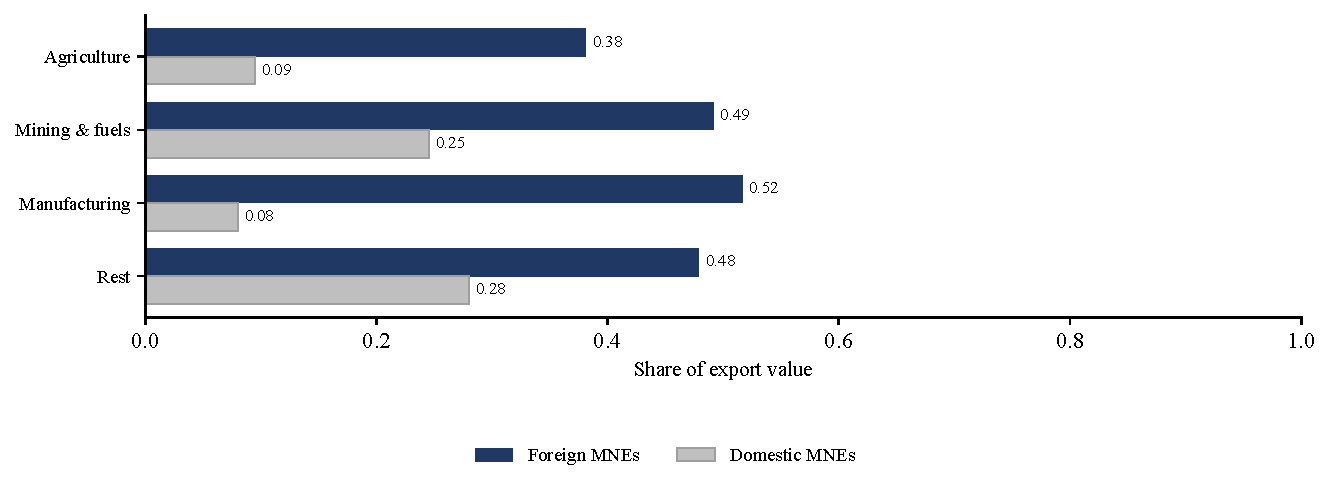
\includegraphics[width=0.8\textwidth,height=0.8\textheight,keepaspectratio]{figures/sectors/fig_wp2_four_sectors.pdf}%
  \caption{Multinational Share of Export Value, by Sector}%
  \label{fig:four_f}%
  \par\vspace{2pt}%
  \parbox{0.92\textwidth}{\footnotesize %
  \textit{Notes:} Shares of export value, all available years pooled. Agriculture: HS 01--24. Mining and fuels: HS 25--27 and 71. Manufacturing: HS 28--97 excluding 71.\\[3pt]%
  \textit{Source:} Authors' calculations based on customs data matched to Orbis and Dun \& Bradstreet.}%
  \end{figure}
% ---- Figure: Foreign-Multinational Share of Export Value, by Exporting Country and Sector
\begin{figure}[H]\centering%
  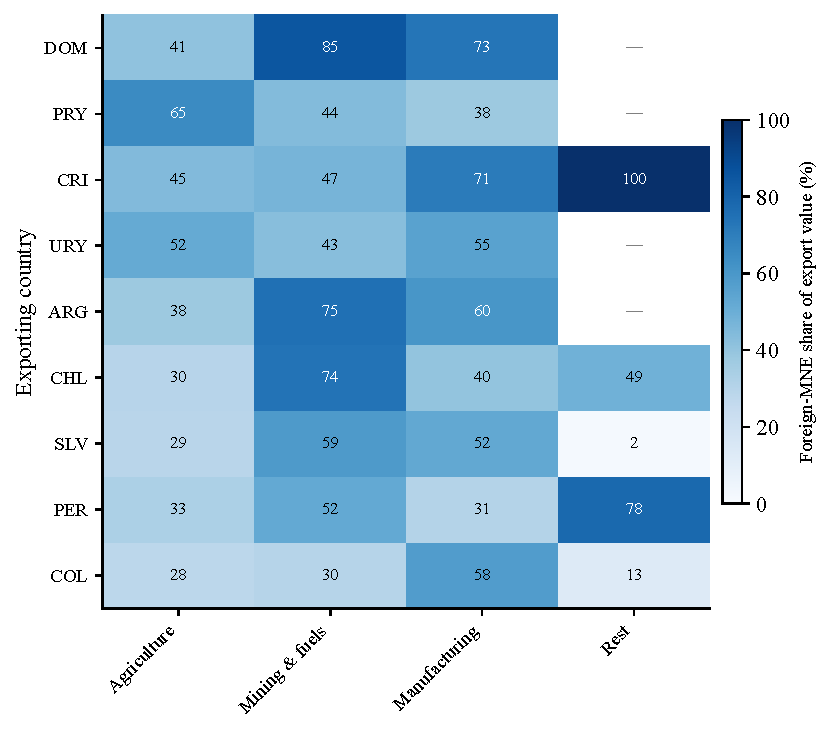
\includegraphics[width=0.8\textwidth,height=0.8\textheight,keepaspectratio]{figures/sectors/fig_wp2_origin_x_sector.pdf}%
  \caption{Foreign-Multinational Share of Export Value, by Exporting Country and Sector}%
  \label{fig:ox_f}%
  \par\vspace{2pt}%
  \parbox{0.92\textwidth}{\footnotesize %
  \textit{Notes:} Percent of each country's export value in each sector shipped by foreign MNEs.\\[3pt]%
  \textit{Source:} Authors' calculations based on customs data matched to Orbis and Dun \& Bradstreet.}%
  \end{figure}
% ---- Table: Exports by Exporting Country and Sector
\begin{table}[H]\centering\small%
  \caption{Exports by Exporting Country and Sector}%
  \label{tab:ox_t}%
  \adjustbox{max width=\textwidth, max totalheight=0.8\textheight}{\begin{tabular}{lrrrrr}
\toprule
Origin & Agriculture & Mining \& fuels & Manufacturing & Rest & All \\
\midrule
\multicolumn{6}{l}{\textit{Panel A: composition of the origin's exports, \% (rows sum to 100)}} \\
ARG & 57.4 & 9.9 & 32.7 & 0.0 & 100.0 \\
CHL & 21.9 & 29.7 & 46.9 & 1.4 & 100.0 \\
COL & 16.3 & 63.4 & 20.3 & 0.0 & 100.0 \\
CRI & 41.5 & 1.0 & 57.5 & 0.0 & 100.0 \\
DOM & 23.1 & 22.8 & 54.1 & 0.0 & 100.0 \\
PER & 19.4 & 61.0 & 19.6 & 0.0 & 100.0 \\
PRY & 85.2 & 1.1 & 13.7 & 0.0 & 100.0 \\
SLV & 22.1 & 3.0 & 74.9 & 0.0 & 100.0 \\
URY & 63.0 & 2.4 & 34.6 & 0.0 & 100.0 \\
All origins & 32.9 & 33.9 & 32.9 & 0.3 & 100.0 \\
\midrule
\multicolumn{6}{l}{\textit{Panel B: foreign-MNE share of export value, \%}} \\
ARG & 37.8 & 75.1 & 60.4 & -- & 48.9 \\
CHL & 29.6 & 73.9 & 39.9 & 48.6 & 47.9 \\
COL & 28.0 & 30.1 & 57.8 & 12.7 & 35.3 \\
CRI & 44.5 & 46.9 & 70.9 & 100.0 & 59.7 \\
DOM & 40.7 & 85.3 & 73.2 & -- & 68.4 \\
PER & 33.0 & 52.2 & 30.6 & 78.0 & 44.2 \\
PRY & 65.0 & 44.1 & 37.9 & -- & 61.1 \\
SLV & 28.9 & 58.8 & 52.5 & 1.5 & 47.4 \\
URY & 51.8 & 42.9 & 55.3 & -- & 52.8 \\
All origins & 38.1 & 49.2 & 51.6 & 47.9 & 46.3 \\
\bottomrule
\end{tabular}
}%
  \par\vspace{3pt}%
  \begin{minipage}{0.95\textwidth}\footnotesize %
  \textit{Notes:} Panel A: composition of each country's exports by sector (rows add to 100). Panel B: percent of each cell's export value shipped by foreign MNEs.\\[3pt]%
  \textit{Source:} Authors' calculations based on customs data matched to Orbis and Dun \& Bradstreet.%
  \end{minipage}%
  \end{table}
% ---- Table: Industry of Matched Exporting Affiliates
\begin{table}[H]\centering\small%
  \caption{Industry of Matched Exporting Affiliates}%
  \label{tab:services}%
  \adjustbox{max width=\textwidth, max totalheight=0.8\textheight}{\begin{tabular}{lr}
\toprule
NAICS sector of the matched exporting affiliate & \% of matched export value \\
\midrule
goods-producing or unknown & 82.4 \\
information, finance, professional, holdings (51--56) & 7.7 \\
wholesale / retail trade (42--45) & 7.4 \\
other services (61--92) & 1.8 \\
transport, logistics (48--49) & 0.6 \\
\bottomrule
\end{tabular}
}%
  \par\vspace{3pt}%
  \begin{minipage}{0.95\textwidth}\footnotesize %
  \textit{Notes:} Percent of matched export value, by NAICS sector of the exporting affiliate. Services are not observed in customs records; the table shows how much of goods exports is shipped by affiliates classified in service industries.\\[3pt]%
  \textit{Source:} Authors' calculations based on customs data matched to Orbis and Dun \& Bradstreet.%
  \end{minipage}%
  \end{table}
% ---- Figure: Exports by US-Parent Multinationals, by Exporting Country and Sector
\begin{figure}[H]\centering%
  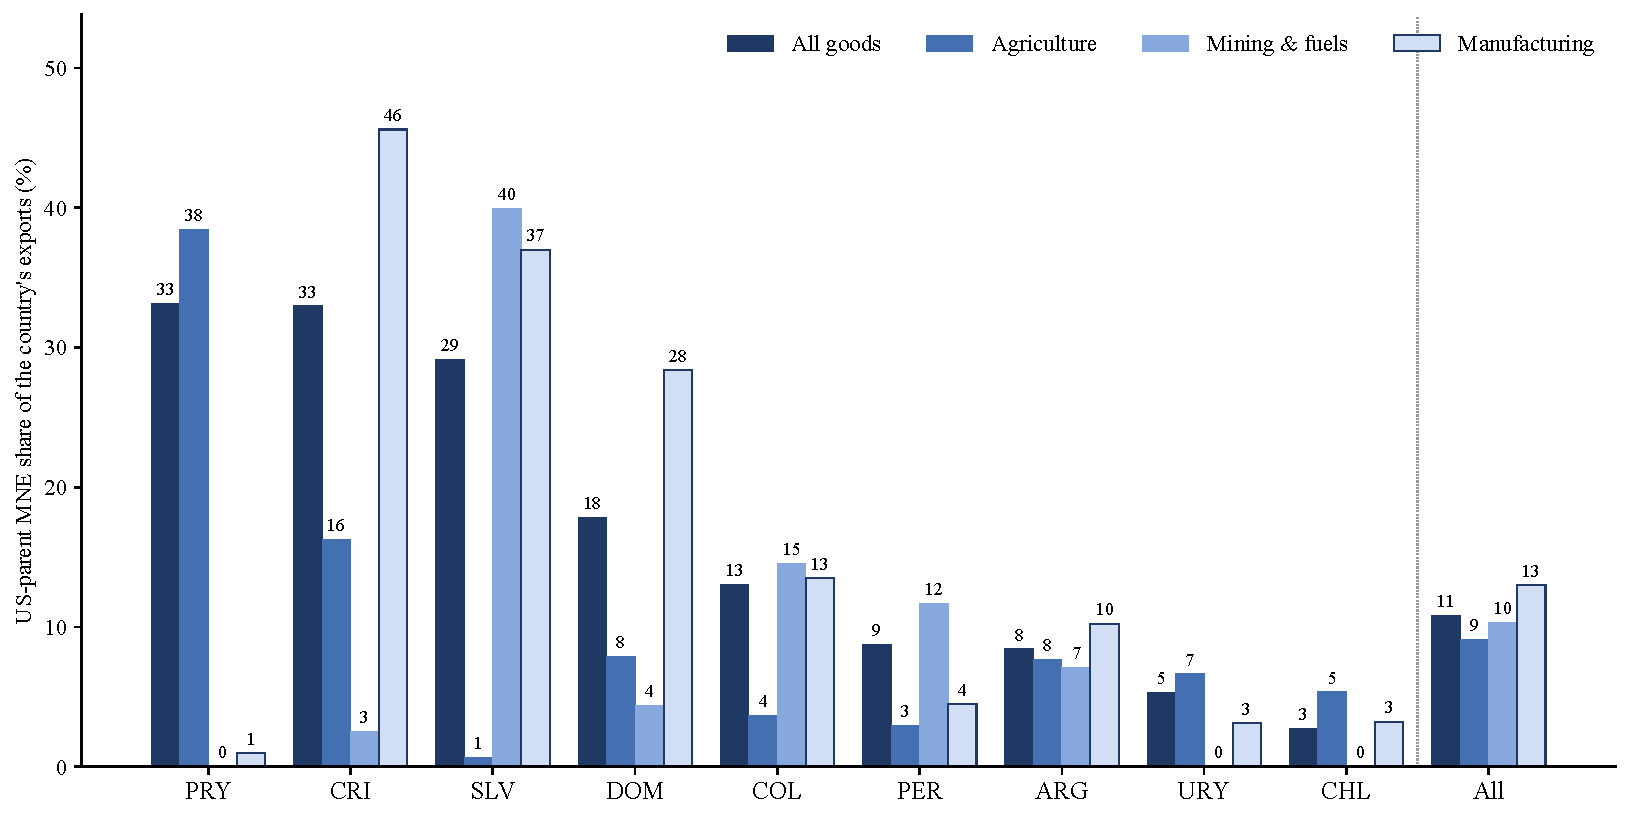
\includegraphics[width=1.0\textwidth,height=0.8\textheight,keepaspectratio]{figures/sectors/fig_wp3_us_share_origin_sector.pdf}%
  \caption{Exports by US-Parent Multinationals, by Exporting Country and Sector}%
  \label{fig:us_ox_sector}%
  \par\vspace{2pt}%
  \parbox{0.92\textwidth}{\footnotesize %
  \textit{Notes:} Percent of each country's exports in each sector shipped by US-parent MNEs, to all destinations.\\[3pt]%
  \textit{Source:} Authors' calculations based on customs data matched to Orbis and Dun \& Bradstreet.}%
  \end{figure}
% ---- Table: Exports by US-Parent Multinationals, by Exporting Country and Sector
\begin{table}[H]\centering\small%
  \caption{Exports by US-Parent Multinationals, by Exporting Country and Sector}%
  \label{tab:us_ox_sector_t}%
  \adjustbox{max width=\textwidth, max totalheight=0.8\textheight}{\begin{tabular}{lrrrrrrrr}
\toprule
 & \multicolumn{4}{c}{US-parent MNE share of the origin's exports in the sector (\%)} & \multicolumn{4}{c}{US-parent MNE exports (US\$bn/yr)} \\
Origin & All goods & Agriculture & Mining \& fuels & Manufacturing & All goods & Agriculture & Mining \& fuels & Manufacturing \\
\midrule
PRY & 33.1 & 38.5 & 0.0 & 1.0 & 2.2 & 2.2 & 0.0 & 0.0 \\
CRI & 33.0 & 16.2 & 2.6 & 45.6 & 3.2 & 0.6 & 0.0 & 2.5 \\
SLV & 29.1 & 0.6 & 39.9 & 37.0 & 1.4 & 0.0 & 0.1 & 1.3 \\
DOM & 17.8 & 7.9 & 4.4 & 28.4 & 1.5 & 0.2 & 0.1 & 1.2 \\
COL & 13.1 & 3.7 & 14.6 & 13.5 & 5.1 & 0.2 & 3.9 & 1.0 \\
PER & 8.8 & 2.9 & 11.7 & 4.5 & 3.2 & 0.2 & 2.8 & 0.3 \\
ARG & 8.4 & 7.7 & 7.1 & 10.2 & 5.4 & 2.7 & 0.5 & 2.2 \\
URY & 5.3 & 6.6 & 0.0 & 3.1 & 0.3 & 0.3 & 0.0 & 0.1 \\
CHL & 2.8 & 5.4 & 0.1 & 3.2 & 0.9 & 0.3 & 0.0 & 0.5 \\
\midrule
All & 10.8 & 9.1 & 10.3 & 13.0 & 23.1 & 6.7 & 7.3 & 9.1 \\
\bottomrule
\end{tabular}
}%
  \par\vspace{3pt}%
  \begin{minipage}{0.95\textwidth}\footnotesize %
  \textit{Notes:} Left panel: percent of each country's exports in the sector shipped by US-parent MNEs. Right panel: exports by US-parent MNEs. Values are annual averages in US\$ billion.\\[3pt]%
  \textit{Source:} Authors' calculations based on customs data matched to Orbis and Dun \& Bradstreet.%
  \end{minipage}%
  \end{table}
% ---- Figure: Share of Foreign-Multinational Exports Shipped to the Parent Country, by Sector
\begin{figure}[H]\centering%
  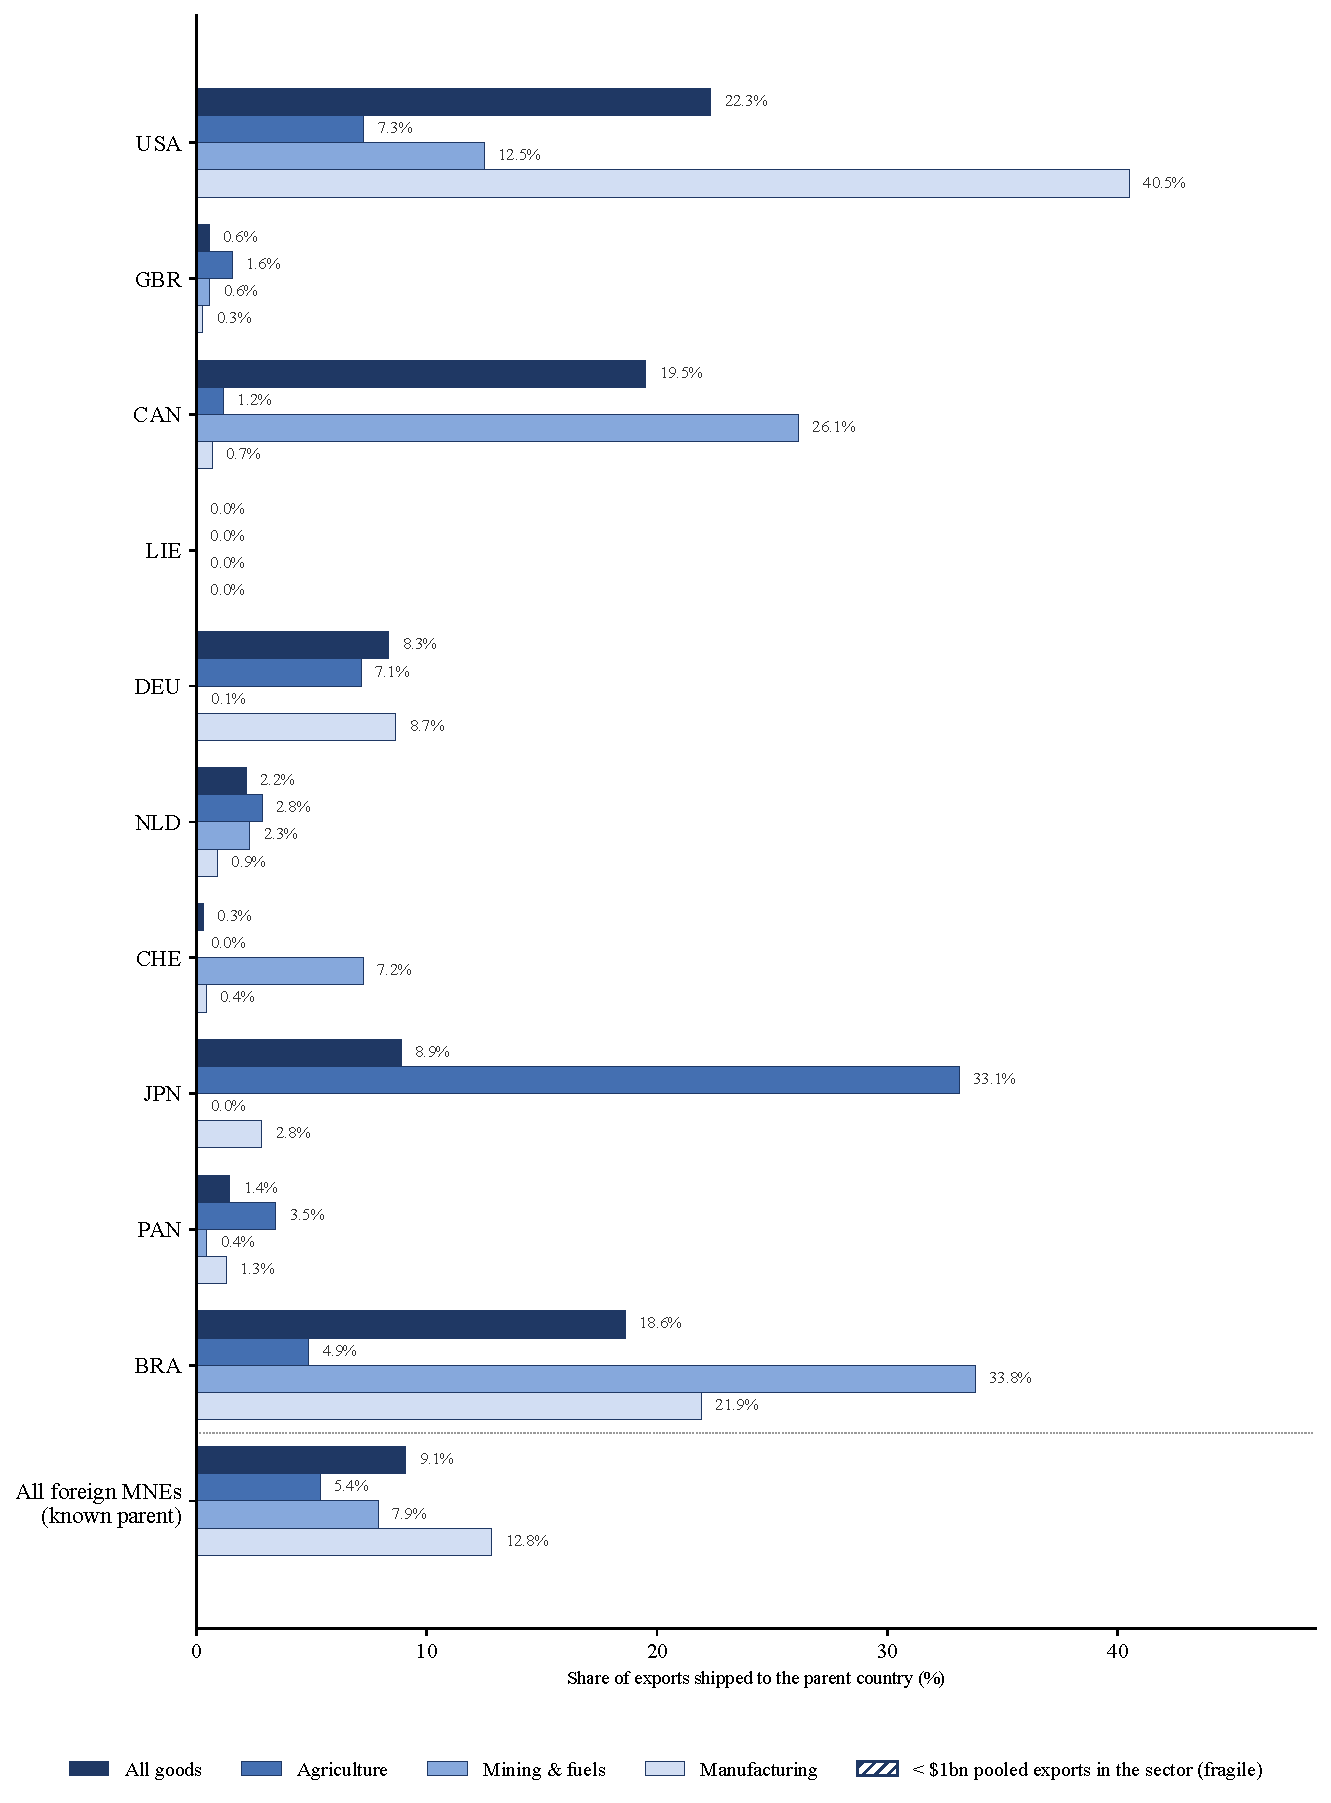
\includegraphics[width=0.95\textwidth,height=0.8\textheight,keepaspectratio]{figures/sectors/fig_wp3_home_share_by_parent_sectors.pdf}%
  \caption{Share of Foreign-Multinational Exports Shipped to the Parent Country, by Sector}%
  \label{fig:home_sectors}%
  \par\vspace{2pt}%
  \parbox{0.92\textwidth}{\footnotesize %
  \textit{Notes:} Percent of each parent country's exports shipped to that same country, by sector. Hatched bars: the parent country's exports in the sector are below US\$1 billion over the period.\\[3pt]%
  \textit{Source:} Authors' calculations based on customs data matched to Orbis and Dun \& Bradstreet.}%
  \end{figure}
% ---- Table: Share of Foreign-Multinational Exports Shipped to the Parent Country, by Sector
\begin{table}[H]\centering\footnotesize%
  \caption{Share of Foreign-Multinational Exports Shipped to the Parent Country, by Sector}%
  \label{tab:home_sectors_t}%
  \adjustbox{max width=\textwidth, max totalheight=0.8\textheight}{\begin{tabular}{lrrrrrrrr}
\toprule
 & \multicolumn{4}{c}{\% of the parent's exports shipped to the parent's country} & \multicolumn{4}{c}{Parent's exports (US\$bn/yr)} \\
Parent & All goods & Agriculture & Mining \& fuels & Manufacturing & All goods & Agriculture & Mining \& fuels & Manufacturing \\
\midrule
USA & 22.3 & 7.3 & 12.5 & 40.5 & 23.1 & 6.7 & 7.3 & 9.1 \\
GBR & 0.6 & 1.6 & 0.6 & 0.3 & 16.7 & 0.7 & 11.9 & 4.2 \\
CAN & 19.5 & 1.2 & 26.1 & 0.7 & 7.4 & 0.4 & 5.7 & 1.3 \\
LIE & 0.0 & 0.0 & 0.0 & 0.0 & 4.9 & 2.2 & 2.0 & 0.7 \\
DEU & 8.3 & 7.1 & 0.1 & 8.7 & 4.6 & 0.8 & 0.0 & 3.7 \\
NLD & 2.2 & 2.8 & 2.3 & 0.9 & 4.4 & 2.7 & 0.1 & 1.5 \\
CHE & 0.3 & 0.0 & 7.2 & 0.4 & 3.9 & 3.1 & 0.1 & 0.7 \\
JPN & 8.9 & 33.1 & 0.0 & 2.8 & 3.5 & 0.6 & 0.0 & 2.9 \\
PAN & 1.4 & 3.5 & 0.4 & 1.3 & 3.0 & 0.6 & 1.0 & 1.3 \\
BRA & 18.6 & 4.9 & 33.8 & 21.9 & 3.0 & 1.1 & 0.7 & 1.3 \\
\midrule
All known-parent foreign MNEs & 9.1 & 5.4 & 7.9 & 12.8 & 97.6 & 27.2 & 34.5 & 35.7 \\
\bottomrule
\end{tabular}
}%
  \par\vspace{3pt}%
  \begin{minipage}{0.95\textwidth}\footnotesize %
  \textit{Notes:} Left panel: percent of each parent country's exports shipped to that same country. Right panel: the parent country's exports. Values are annual averages in US\$ billion.\\[3pt]%
  \textit{Source:} Authors' calculations based on customs data matched to Orbis and Dun \& Bradstreet.%
  \end{minipage}%
  \end{table}
% ---- Figure: Exports to the United States, by Type of Exporter and Exporting Country
\begin{figure}[H]\centering%
  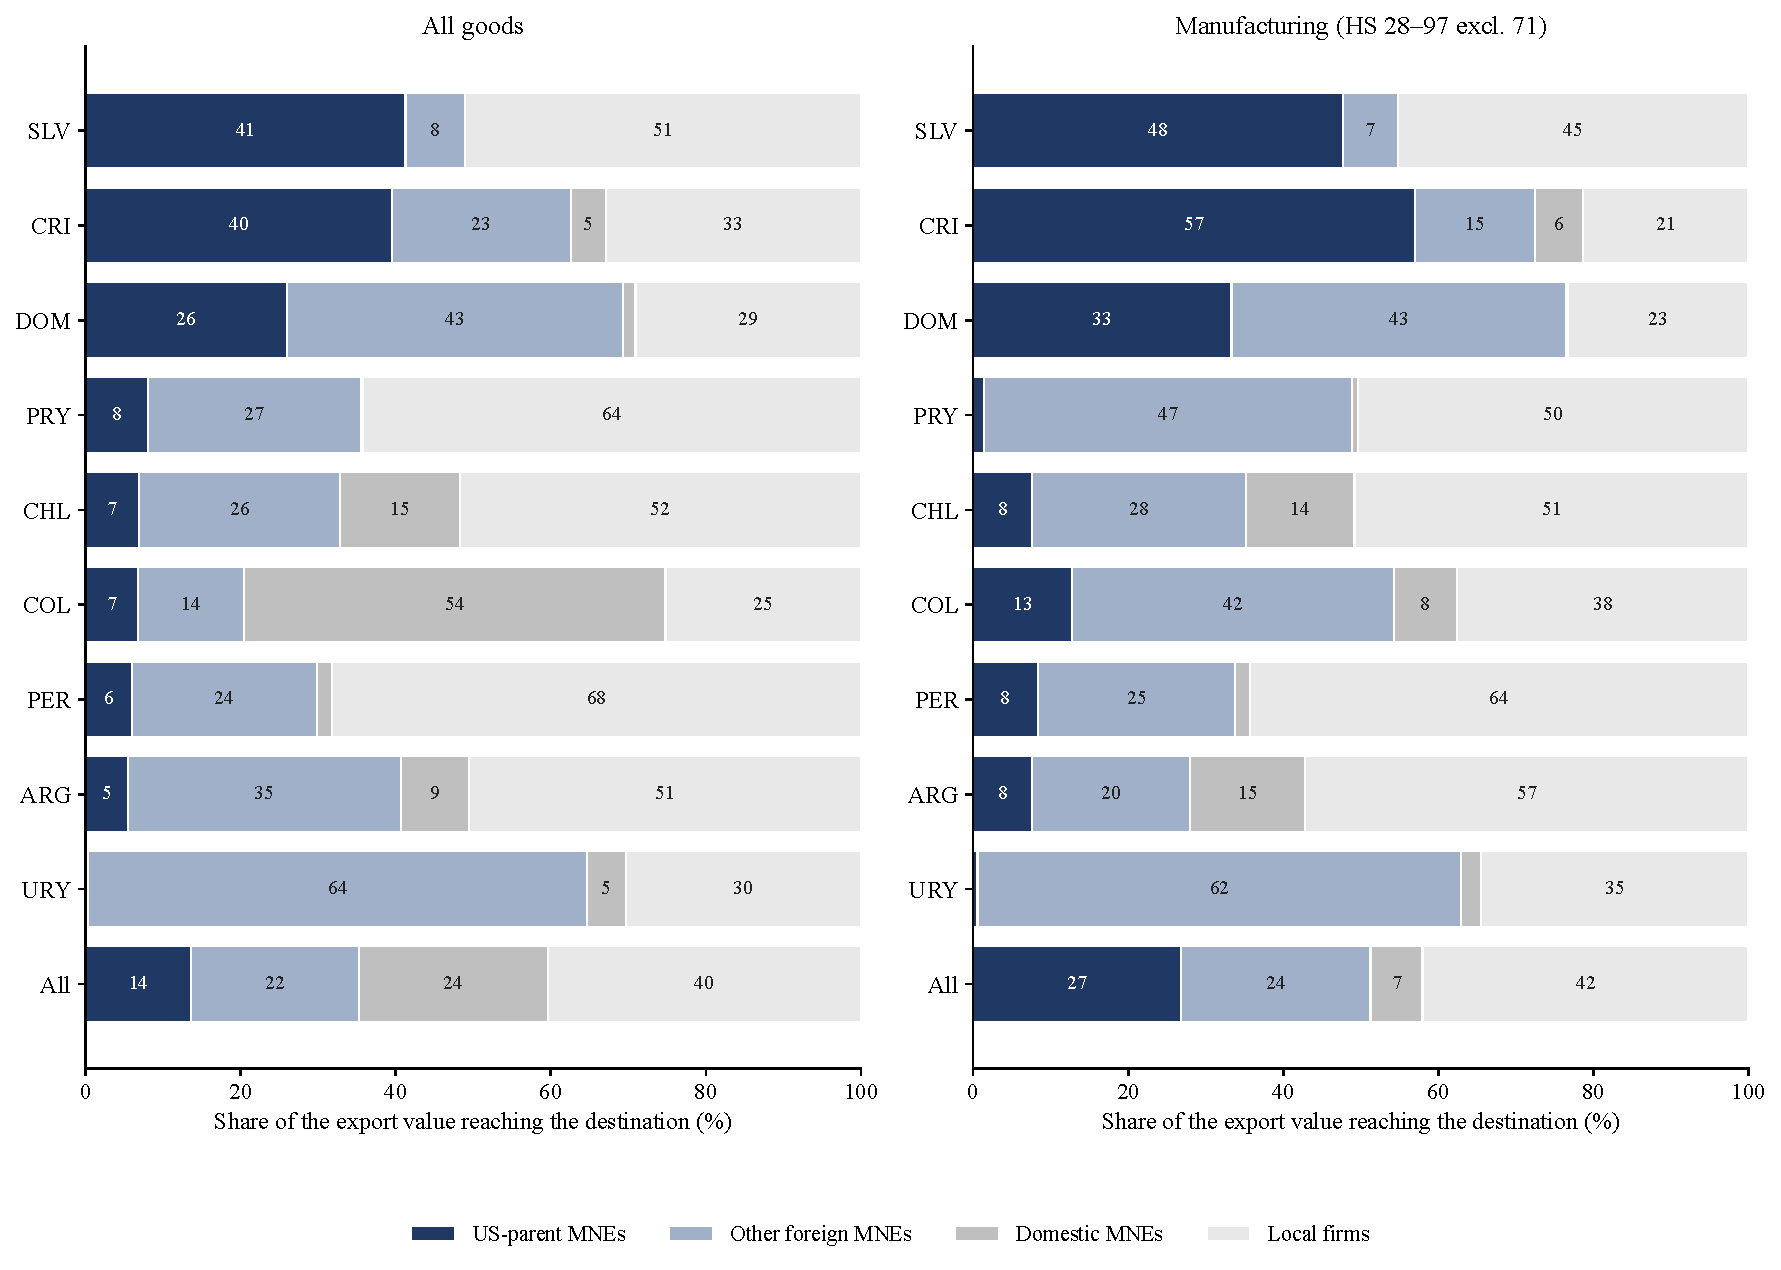
\includegraphics[width=1.0\textwidth,height=0.8\textheight,keepaspectratio]{figures/sectors/fig_wp3_to_usa_carriers_total_manuf.pdf}%
  \caption{Exports to the United States, by Type of Exporter and Exporting Country}%
  \label{fig:to_usa_tm}%
  \par\vspace{2pt}%
  \parbox{0.92\textwidth}{\footnotesize %
  \textit{Notes:} Percent of each country's exports to the United States, by type of exporter. Left: all goods. Right: manufacturing.\\[3pt]%
  \textit{Source:} Authors' calculations based on customs data matched to Orbis and Dun \& Bradstreet.}%
  \end{figure}
% ---- Table: Exports to the United States, by Type of Exporter and Sector
\begin{table}[H]\centering\small%
  \caption{Exports to the United States, by Type of Exporter and Sector}%
  \label{tab:to_usa_sec}%
  \adjustbox{max width=\textwidth, max totalheight=0.8\textheight}{\begin{tabular}{lrrrrr}
\toprule
Sector & Exports to the USA (US\$bn/yr) & US-parent MNEs (\%) & Other foreign MNEs (\%) & Domestic MNEs (\%) & Local firms (\%) \\
\midrule
\midrule
All goods & 40.0 & 13.6 & 21.6 & 24.4 & 40.4 \\
Agriculture & 10.7 & 4.8 & 28.0 & 9.2 & 58.0 \\
Mining \& fuels & 14.6 & 6.6 & 14.8 & 52.0 & 26.6 \\
Manufacturing & 14.5 & 26.8 & 24.4 & 6.7 & 42.1 \\
Rest & 0.1 & 40.0 & 38.4 & 4.5 & 17.1 \\
\bottomrule
\end{tabular}
}%
  \par\vspace{3pt}%
  \begin{minipage}{0.95\textwidth}\footnotesize %
  \textit{Notes:} Percent of each sector's exports to the United States, by type of exporter. Values are annual averages in US\$ billion.\\[3pt]%
  \textit{Source:} Authors' calculations based on customs data matched to Orbis and Dun \& Bradstreet.%
  \end{minipage}%
  \end{table}
% ---- Table: Multinational Presence and Exports by Sector: Intensive Margin
\begin{table}[H]\centering\small%
  \caption{Multinational Presence and Exports by Sector: Intensive Margin}%
  \label{tab:f5sum}%
  \adjustbox{max width=\textwidth, max totalheight=0.8\textheight}{\begin{tabular}{lcccc} \hline
Sample & All goods & Agriculture & Mining \& fuels & Manufacturing \\ \hline
\multicolumn{5}{l}{\textit{Panel A. Dependent variable: $\ln$ exports, all firms}} \\
\multicolumn{5}{l}{\footnotesize Fixed effects: origin $\times$ year, destination $\times$ year, product} \\
\quad $\ln$(\# foreign MNEs) & 1.2129*** & 1.2954*** & 1.1301*** & 1.1644*** \\
 & (0.0285) & (0.0275) & (0.1799) & (0.0358) \\
\quad $\ln$(\# domestic MNEs) & 0.4382*** & 0.5233*** & 0.3172 & 0.3833*** \\
 & (0.0259) & (0.0266) & (0.2062) & (0.0319) \\
\quad Observations & 113,422 & 25,437 & 1,417 & 85,453 \\
\multicolumn{5}{l}{\footnotesize Fixed effects: origin $\times$ destination $\times$ product, origin $\times$ destination $\times$ year} \\
\quad $\ln$(\# foreign MNEs) & 0.4506*** & 0.4625*** & 0.2479 & 0.4435*** \\
 & (0.0124) & (0.0188) & (0.1778) & (0.0148) \\
\quad $\ln$(\# domestic MNEs) & 0.2214*** & 0.2831*** & 0.3216* & 0.1904*** \\
 & (0.0151) & (0.0234) & (0.1639) & (0.0175) \\
\quad Observations & 98,223 & 22,002 & 1,027 & 73,318 \\
\midrule
\multicolumn{5}{l}{\textit{Panel B. Dependent variable: $\ln$ exports, non-MNE firms}} \\
\multicolumn{5}{l}{\footnotesize Fixed effects: origin $\times$ year, destination $\times$ year, product} \\
\quad $\ln$(\# foreign MNEs) & 1.1331*** & 1.2191*** & 0.9420*** & 1.0546*** \\
 & (0.0375) & (0.0363) & (0.2641) & (0.0493) \\
\quad $\ln$(\# domestic MNEs) & 0.4707*** & 0.5676*** & -0.6594 & 0.4194*** \\
 & (0.0341) & (0.0339) & (0.4830) & (0.0419) \\
\quad Observations & 93,010 & 22,503 & 995 & 68,534 \\
\multicolumn{5}{l}{\footnotesize Fixed effects: origin $\times$ destination $\times$ product, origin $\times$ destination $\times$ year} \\
\quad $\ln$(\# foreign MNEs) & 0.2413*** & 0.3602*** & -0.1512 & 0.1865*** \\
 & (0.0217) & (0.0292) & (0.3320) & (0.0250) \\
\quad $\ln$(\# domestic MNEs) & 0.1250*** & 0.2461*** & -0.7273 & 0.0742*** \\
 & (0.0218) & (0.0341) & (0.6536) & (0.0238) \\
\quad Observations & 81,563 & 19,535 & 726 & 59,772 \\
\hline
\end{tabular}
}%
  \par\vspace{3pt}%
  \begin{minipage}{0.95\textwidth}\footnotesize %
  \textit{Notes:} Observations are origin--destination--HS6--year cells. Dependent variable: $\ln$ exports of the cell (Panel A) and of the non-MNE firms in the cell (Panel B). Regressors: $\ln$ number of foreign and of domestic MNEs; cells with at least one of each. Blank: too few observations. Standard errors clustered by origin--destination pair in parentheses. *** $p<0.01$, ** $p<0.05$, * $p<0.1$.\\[3pt]%
  \textit{Source:} Authors' calculations based on customs data matched to Orbis and Dun \& Bradstreet.%
  \end{minipage}%
  \end{table}
% ---- Table: Distance and Firm Exports, by Sector
\begin{table}[H]\centering\small%
  \caption{Distance and Firm Exports, by Sector}%
  \label{tab:f6sum}%
  \adjustbox{max width=\textwidth, max totalheight=0.8\textheight}{\begin{tabular}{lcccc} \hline
Dep.\ var.: $\ln$ firm exports & All goods & Agriculture & Mining \& fuels & Manufacturing \\ \hline
\multicolumn{5}{l}{\footnotesize Origin, destination, year and product FE} \\
\quad $\ln$ distance & -0.1645*** & -0.2135*** & -0.0926 & -0.1510*** \\
 & (0.0454) & (0.0748) & (0.0819) & (0.0454) \\
\quad $\ln$ distance $\times$ foreign MNE & 0.0487*** & 0.0366*** & 0.0566*** & 0.0515*** \\
 & (0.0041) & (0.0034) & (0.0086) & (0.0048) \\
\quad $\ln$ distance $\times$ domestic MNE & 0.0318*** & 0.0187*** & 0.0706*** & 0.0388*** \\
 & (0.0042) & (0.0046) & (0.0180) & (0.0052) \\
\quad Observations & 5,081,547 & 1,045,009 & 79,938 & 3,917,960 \\
\midrule
\multicolumn{5}{l}{\footnotesize Origin $\times$ year, destination $\times$ year and product FE} \\
\quad $\ln$ distance & -0.1853*** & -0.2285*** & -0.1001 & -0.1742*** \\
 & (0.0460) & (0.0711) & (0.0828) & (0.0459) \\
\quad $\ln$ distance $\times$ foreign MNE & 0.0483*** & 0.0358*** & 0.0557*** & 0.0512*** \\
 & (0.0040) & (0.0034) & (0.0087) & (0.0048) \\
\quad $\ln$ distance $\times$ domestic MNE & 0.0318*** & 0.0182*** & 0.0673*** & 0.0390*** \\
 & (0.0042) & (0.0046) & (0.0183) & (0.0052) \\
\quad Observations & 5,081,360 & 1,044,787 & 79,612 & 3,917,765 \\
\hline
\end{tabular}
}%
  \par\vspace{3pt}%
  \begin{minipage}{0.95\textwidth}\footnotesize %
  \textit{Notes:} Observations are firm--destination--HS6--year cells. Dependent variable: $\ln$ exports. Non-MNE firms are the omitted group. Standard errors clustered by origin--destination pair in parentheses. *** $p<0.01$, ** $p<0.05$, * $p<0.1$.\\[3pt]%
  \textit{Source:} Authors' calculations based on customs data matched to Orbis and Dun \& Bradstreet.%
  \end{minipage}%
  \end{table}
\clearpage\part{Agriculture}

\section{Fact 1: Multinationals Account for a Large Share of Exports}\label{sec:f1_agro}
% ---- Figure: Agriculture: Multinational Share of Export Value, by Exporting Country
\begin{figure}[H]\centering%
  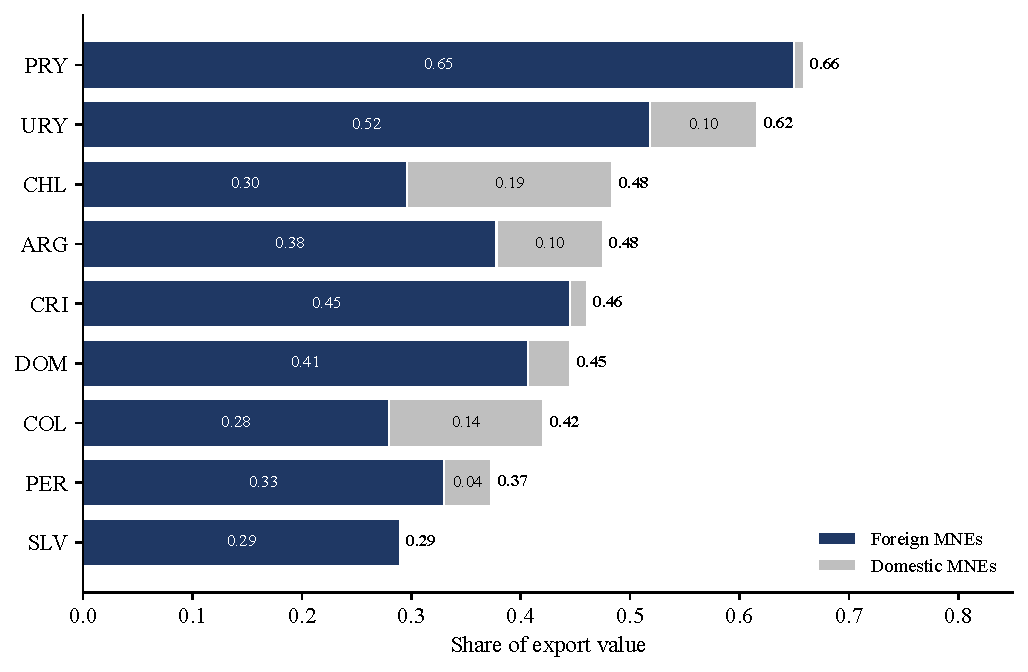
\includegraphics[width=0.8\textwidth,height=0.8\textheight,keepaspectratio]{figures/agro/fig_wp0_fig1_origin.pdf}%
  \caption{Agriculture: Multinational Share of Export Value, by Exporting Country}%
  \label{fig:f1_agro}%
  \par\vspace{2pt}%
  \parbox{0.92\textwidth}{\footnotesize %
  \textit{Notes:} Shares of agricultural export value (HS 01--24), all available years pooled. The figure at the end of each bar is the total MNE share.\\[3pt]%
  \textit{Source:} Authors' calculations based on customs data matched to Orbis and Dun \& Bradstreet.}%
  \end{figure}
% ---- Table: Agriculture: Multinational Share of Export Value, by Exporting Country
\begin{table}[H]\centering\small%
  \caption{Agriculture: Multinational Share of Export Value, by Exporting Country}%
  \label{tab:f1n_agro}%
  \adjustbox{max width=\textwidth, max totalheight=0.8\textheight}{\begin{tabular}{lrrrr}
\toprule
Origin & Foreign & Domestic & All MNEs & Value (US\$bn/yr) \\
\midrule
PRY & 0.650 & 0.009 & 0.659 & 6.2 \\
URY & 0.518 & 0.098 & 0.616 & 4.4 \\
CHL & 0.296 & 0.187 & 0.484 & 7.5 \\
ARG & 0.378 & 0.097 & 0.475 & 38.1 \\
CRI & 0.445 & 0.015 & 0.461 & 4.3 \\
DOM & 0.407 & 0.039 & 0.446 & 2.0 \\
COL & 0.280 & 0.141 & 0.421 & 7.2 \\
PER & 0.330 & 0.044 & 0.373 & 8.1 \\
SLV & 0.289 & 0.000 & 0.289 & 1.1 \\
\midrule
All & 0.381 & 0.095 & 0.476 & 78.9 \\
\bottomrule
\end{tabular}
}%
  \par\vspace{3pt}%
  \begin{minipage}{0.95\textwidth}\footnotesize %
  \textit{Notes:} Shares of agricultural export value (HS 01--24), all available years pooled. Values are annual averages in US\$ billion.\\[3pt]%
  \textit{Source:} Authors' calculations based on customs data matched to Orbis and Dun \& Bradstreet.%
  \end{minipage}%
  \end{table}

\subsection{By Parent Country}
% ---- Figure: Agriculture: Multinational Share of Export Value, by Exporting Country and Parent Country
\begin{figure}[H]\centering%
  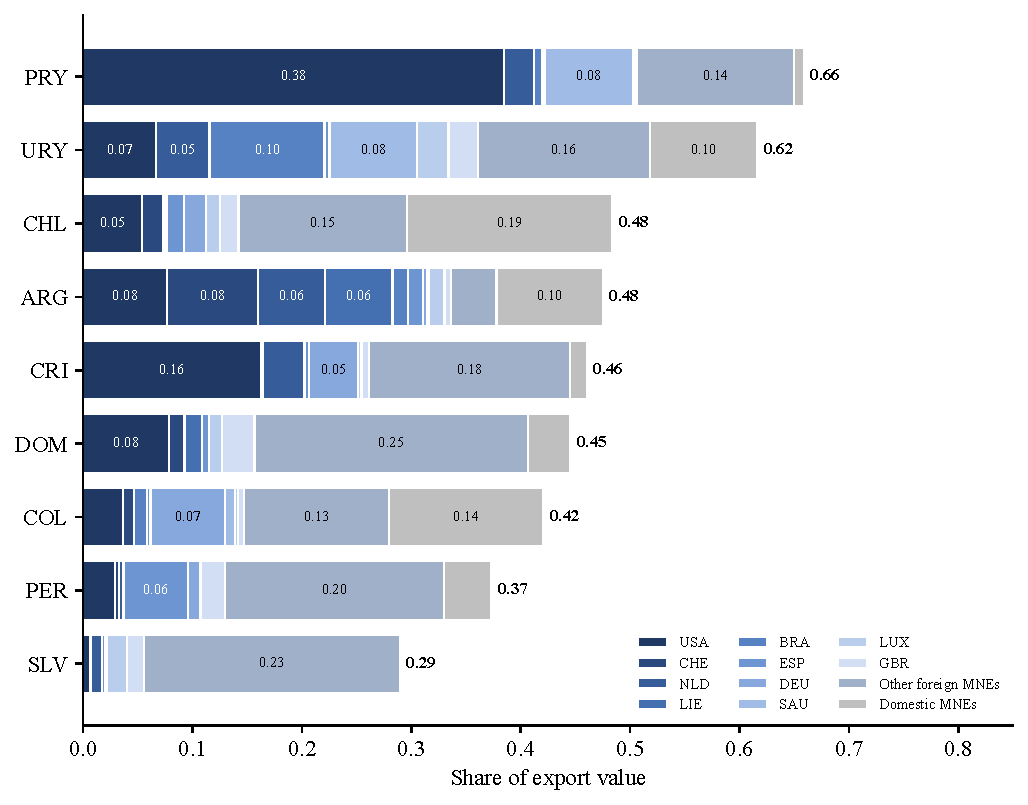
\includegraphics[width=0.92\textwidth,height=0.8\textheight,keepaspectratio]{figures/agro/fig_wp1a_origin_by_parent.pdf}%
  \caption{Agriculture: Multinational Share of Export Value, by Exporting Country and Parent Country}%
  \label{fig:f1p_agro}%
  \par\vspace{2pt}%
  \parbox{0.92\textwidth}{\footnotesize %
  \textit{Notes:} Shares of agricultural export value (HS 01--24), all available years pooled. Foreign MNEs split by country of the ultimate parent; the ten largest parent countries are shown separately.\\[3pt]%
  \textit{Source:} Authors' calculations based on customs data matched to Orbis and Dun \& Bradstreet.}%
  \end{figure}
% ---- Table: Agriculture: Multinational Share of Export Value, by Exporting Country and Parent Country
\begin{table}[H]\centering\small%
  \caption{Agriculture: Multinational Share of Export Value, by Exporting Country and Parent Country}%
  \label{tab:f1pn_agro}%
  \adjustbox{max width=\textwidth, max totalheight=0.8\textheight}{\begin{tabular}{lcccccccccccccc}
\toprule
Origin & USA & CHE & NLD & LIE & BRA & ESP & DEU & SAU & LUX & GBR & Other & Domestic & All MNEs & Value (US\$bn/yr) \\
\midrule
PRY & 0.385 & 0.000 & 0.027 & 0.000 & 0.008 & 0.002 & 0.000 & 0.081 & 0.000 & 0.002 & 0.144 & 0.009 & 0.659 & 6.2 \\
URY & 0.066 & 0.000 & 0.049 & 0.001 & 0.104 & 0.004 & 0.000 & 0.080 & 0.028 & 0.027 & 0.157 & 0.098 & 0.616 & 4.4 \\
CHL & 0.054 & 0.020 & 0.000 & 0.002 & 0.001 & 0.015 & 0.020 & 0.000 & 0.012 & 0.017 & 0.154 & 0.187 & 0.484 & 7.5 \\
ARG & 0.077 & 0.083 & 0.062 & 0.061 & 0.014 & 0.014 & 0.004 & 0.002 & 0.014 & 0.006 & 0.042 & 0.097 & 0.475 & 38.1 \\
CRI & 0.162 & 0.002 & 0.038 & 0.000 & 0.000 & 0.004 & 0.045 & 0.000 & 0.003 & 0.007 & 0.184 & 0.015 & 0.461 & 4.3 \\
DOM & 0.079 & 0.014 & 0.000 & 0.016 & 0.000 & 0.007 & 0.000 & 0.000 & 0.012 & 0.029 & 0.250 & 0.039 & 0.446 & 2.0 \\
COL & 0.037 & 0.010 & 0.000 & 0.000 & 0.012 & 0.003 & 0.068 & 0.009 & 0.003 & 0.006 & 0.132 & 0.141 & 0.421 & 7.2 \\
PER & 0.029 & 0.004 & 0.004 & 0.000 & 0.000 & 0.059 & 0.011 & 0.000 & 0.000 & 0.022 & 0.200 & 0.044 & 0.373 & 8.1 \\
SLV & 0.006 & 0.001 & 0.010 & 0.000 & 0.000 & 0.003 & 0.001 & 0.000 & 0.019 & 0.015 & 0.233 & 0.000 & 0.289 & 1.1 \\
\bottomrule
\end{tabular}
}%
  \par\vspace{3pt}%
  \begin{minipage}{0.95\textwidth}\footnotesize %
  \textit{Notes:} Shares of agricultural export value (HS 01--24), all available years pooled. Other: all remaining foreign parents. Values are annual averages in US\$ billion.\\[3pt]%
  \textit{Source:} Authors' calculations based on customs data matched to Orbis and Dun \& Bradstreet.%
  \end{minipage}%
  \end{table}
% ---- Figure: Agriculture: Export Value by Exporting Country and Parent Country
\begin{figure}[H]\centering%
  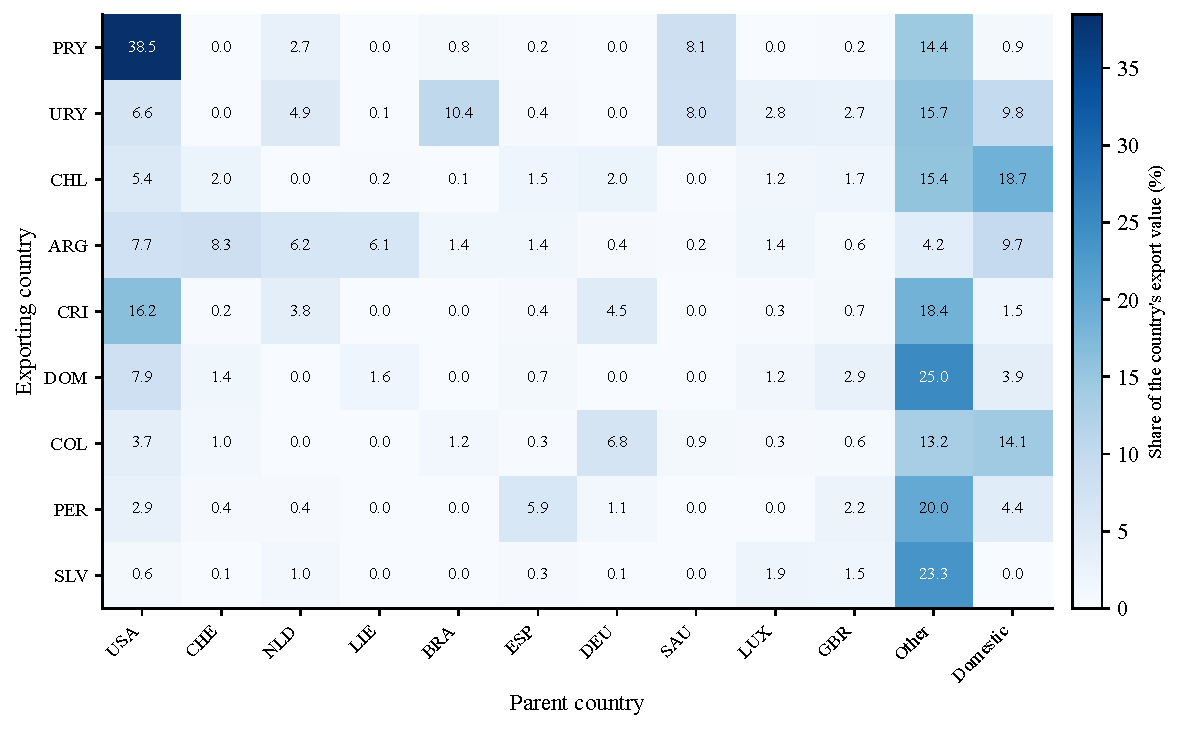
\includegraphics[width=0.9\textwidth,height=0.8\textheight,keepaspectratio]{figures/agro/fig_wp1a_origin_x_parent_heatmap.pdf}%
  \caption{Agriculture: Export Value by Exporting Country and Parent Country}%
  \label{fig:f1hm_agro}%
  \par\vspace{2pt}%
  \parbox{0.92\textwidth}{\footnotesize %
  \textit{Notes:} Percent of each country's agricultural export value, by country of the ultimate parent of the exporter.\\[3pt]%
  \textit{Source:} Authors' calculations based on customs data matched to Orbis and Dun \& Bradstreet.}%
  \end{figure}

\section{Fact 2: Foreign Multinationals Specialize in Complex Products, Domestic Multinationals in Primary Goods}\label{sec:f2_agro}

\subsection{Product Complexity and Technology}
% ---- Figure: Agriculture: Multinational Share of Export Value, by Product Complexity Quintile
\begin{figure}[H]\centering%
  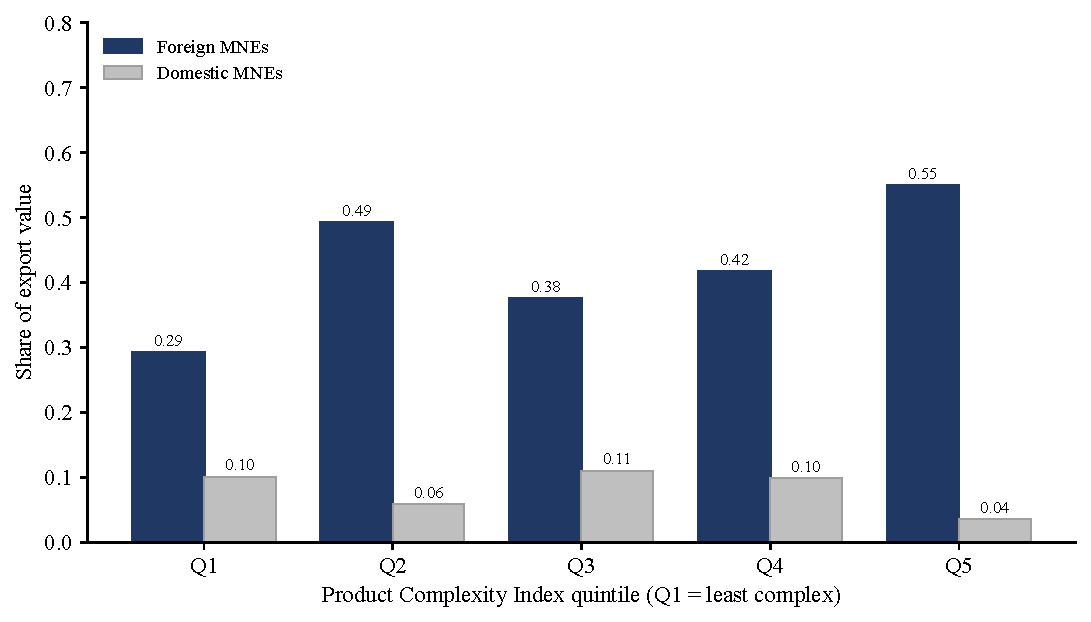
\includegraphics[width=0.78\textwidth,height=0.8\textheight,keepaspectratio]{figures/agro/fig_wp0_fig2_pci.pdf}%
  \caption{Agriculture: Multinational Share of Export Value, by Product Complexity Quintile}%
  \label{fig:pci_agro}%
  \par\vspace{2pt}%
  \parbox{0.92\textwidth}{\footnotesize %
  \textit{Notes:} Shares of agricultural export value (HS 01--24), all available years pooled. Quintiles of the Hausmann--Hidalgo Product Complexity Index across HS6 products (Q1 = least complex).\\[3pt]%
  \textit{Source:} Authors' calculations based on customs data matched to Orbis and Dun \& Bradstreet.}%
  \end{figure}
% ---- Figure: Agriculture: Multinational Share of Export Value, by Technology Class
\begin{figure}[H]\centering%
  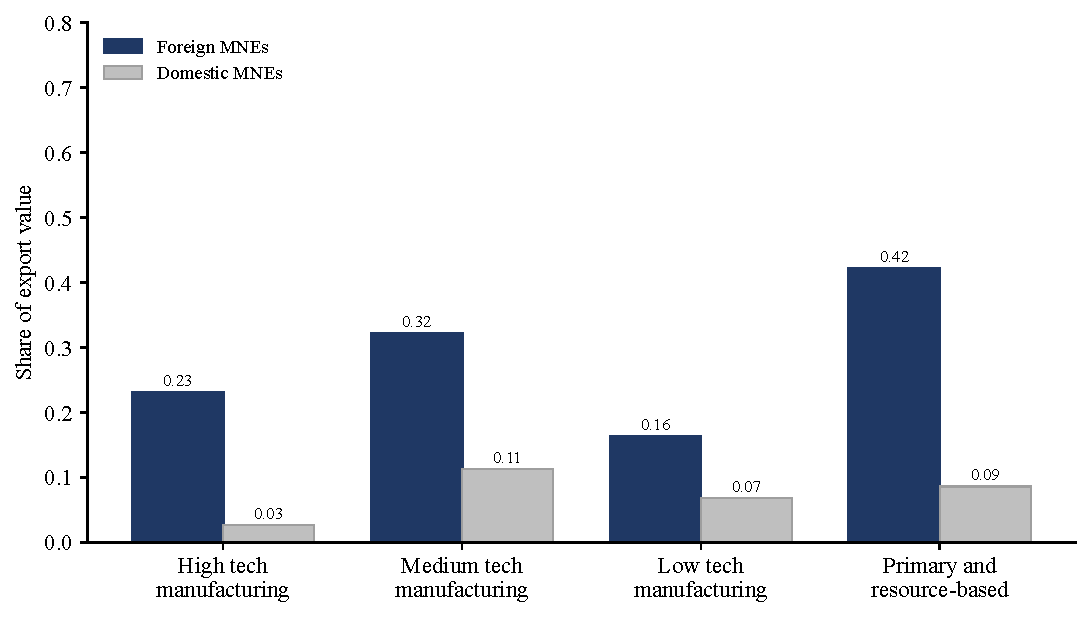
\includegraphics[width=0.78\textwidth,height=0.8\textheight,keepaspectratio]{figures/agro/fig_wp0_fig3_lall.pdf}%
  \caption{Agriculture: Multinational Share of Export Value, by Technology Class}%
  \label{fig:lall_agro}%
  \par\vspace{2pt}%
  \parbox{0.92\textwidth}{\footnotesize %
  \textit{Notes:} Shares of agricultural export value (HS 01--24), all available years pooled. Lall (2000) technology classes: primary and resource-based products, and low-, medium- and high-technology manufactures.\\[3pt]%
  \textit{Source:} Authors' calculations based on customs data matched to Orbis and Dun \& Bradstreet.}%
  \end{figure}

\subsection{By Parent Country}
% ---- Figure: Agriculture: Multinational Share of Export Value, by Product Complexity Quintile and Parent Country
\begin{figure}[H]\centering%
  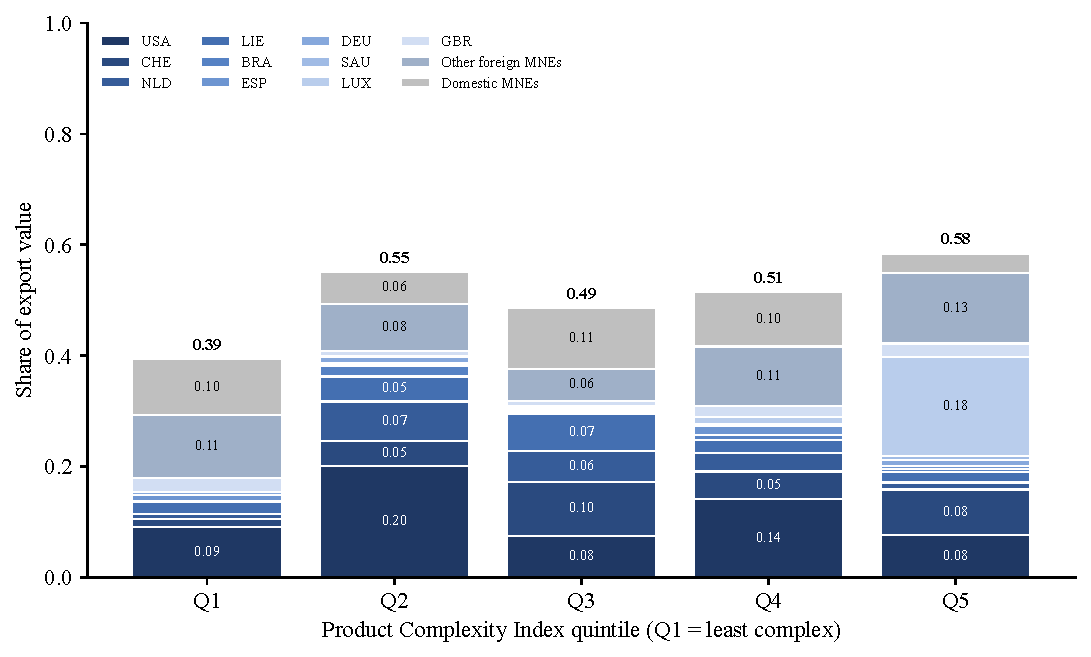
\includegraphics[width=0.92\textwidth,height=0.8\textheight,keepaspectratio]{figures/agro/fig_wp1a_pci_by_parent.pdf}%
  \caption{Agriculture: Multinational Share of Export Value, by Product Complexity Quintile and Parent Country}%
  \label{fig:pci_p_agro}%
  \par\vspace{2pt}%
  \parbox{0.92\textwidth}{\footnotesize %
  \textit{Notes:} Shares of agricultural export value (HS 01--24), all available years pooled. Foreign MNEs split by country of the ultimate parent. Quintiles of the Hausmann--Hidalgo Product Complexity Index across HS6 products (Q1 = least complex).\\[3pt]%
  \textit{Source:} Authors' calculations based on customs data matched to Orbis and Dun \& Bradstreet.}%
  \end{figure}
% ---- Table: Agriculture: Multinational Share of Export Value, by Product Complexity Quintile and Parent Country
\begin{table}[H]\centering\small%
  \caption{Agriculture: Multinational Share of Export Value, by Product Complexity Quintile and Parent Country}%
  \label{tab:pci_pn_agro}%
  \adjustbox{max width=\textwidth, max totalheight=0.8\textheight}{\begin{tabular}{lcccccccccccccc}
\toprule
PCI quintile & USA & CHE & NLD & LIE & BRA & ESP & DEU & SAU & LUX & GBR & Other & Domestic & All MNEs & Value (US\$bn/yr) \\
\midrule
Q1 & 0.091 & 0.014 & 0.009 & 0.022 & 0.001 & 0.012 & 0.005 & 0.000 & 0.000 & 0.025 & 0.113 & 0.101 & 0.394 & 4.5 \\
Q2 & 0.201 & 0.045 & 0.071 & 0.045 & 0.020 & 0.005 & 0.011 & 0.001 & 0.001 & 0.009 & 0.085 & 0.059 & 0.551 & 15.8 \\
Q3 & 0.075 & 0.097 & 0.056 & 0.067 & 0.004 & 0.004 & 0.004 & 0.001 & 0.000 & 0.009 & 0.058 & 0.110 & 0.486 & 17.8 \\
Q4 & 0.142 & 0.049 & 0.033 & 0.024 & 0.009 & 0.015 & 0.004 & 0.000 & 0.013 & 0.019 & 0.108 & 0.098 & 0.515 & 8.3 \\
Q5 & 0.076 & 0.083 & 0.013 & 0.019 & 0.006 & 0.005 & 0.011 & 0.006 & 0.180 & 0.024 & 0.127 & 0.035 & 0.584 & 2.4 \\
\bottomrule
\end{tabular}
}%
  \par\vspace{3pt}%
  \begin{minipage}{0.95\textwidth}\footnotesize %
  \textit{Notes:} Shares of agricultural export value (HS 01--24), all available years pooled. Other: all remaining foreign parents. Values are annual averages in US\$ billion.\\[3pt]%
  \textit{Source:} Authors' calculations based on customs data matched to Orbis and Dun \& Bradstreet.%
  \end{minipage}%
  \end{table}
% ---- Figure: Agriculture: Multinational Share of Export Value, by Technology Class and Parent Country
\begin{figure}[H]\centering%
  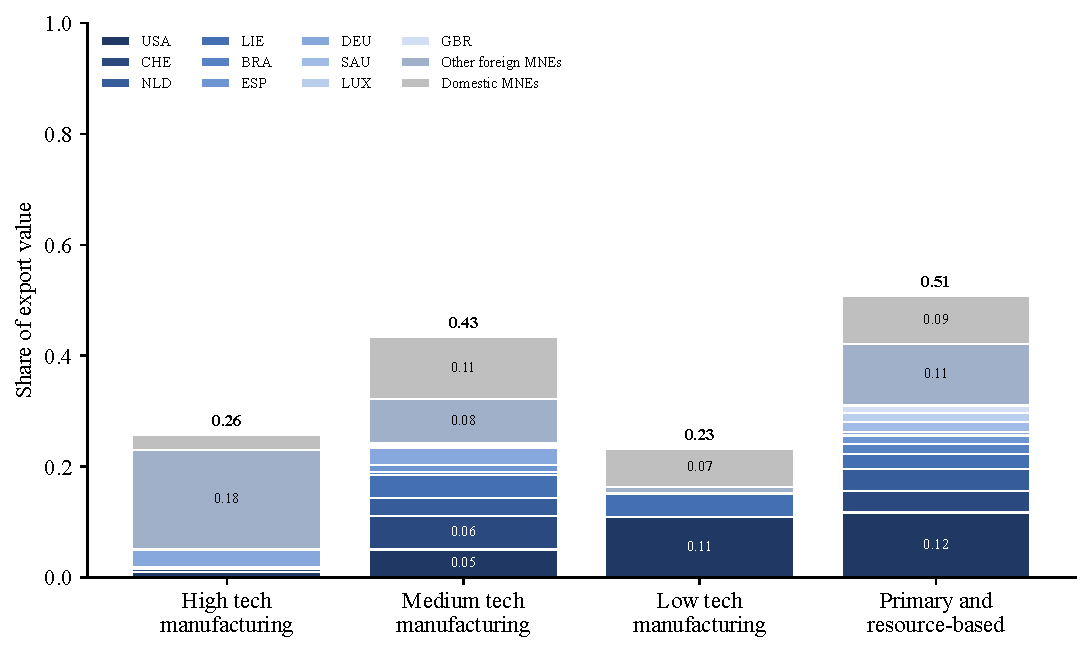
\includegraphics[width=0.92\textwidth,height=0.8\textheight,keepaspectratio]{figures/agro/fig_wp1a_lall_by_parent.pdf}%
  \caption{Agriculture: Multinational Share of Export Value, by Technology Class and Parent Country}%
  \label{fig:lall_p_agro}%
  \par\vspace{2pt}%
  \parbox{0.92\textwidth}{\footnotesize %
  \textit{Notes:} Shares of agricultural export value (HS 01--24), all available years pooled. Foreign MNEs split by country of the ultimate parent. Lall (2000) technology classes: primary and resource-based products, and low-, medium- and high-technology manufactures.\\[3pt]%
  \textit{Source:} Authors' calculations based on customs data matched to Orbis and Dun \& Bradstreet.}%
  \end{figure}
% ---- Table: Agriculture: Multinational Share of Export Value, by Technology Class and Parent Country
\begin{table}[H]\centering\small%
  \caption{Agriculture: Multinational Share of Export Value, by Technology Class and Parent Country}%
  \label{tab:lall_pn_agro}%
  \adjustbox{max width=\textwidth, max totalheight=0.8\textheight}{\begin{tabular}{lcccccccccccccc}
\toprule
Technology category & USA & CHE & NLD & LIE & BRA & ESP & DEU & SAU & LUX & GBR & Other & Domestic & All MNEs & Value (US\$bn/yr) \\
\midrule
High tech manufacturing & 0.009 & 0.005 & 0.001 & 0.000 & 0.001 & 0.003 & 0.030 & 0.000 & 0.000 & 0.001 & 0.180 & 0.026 & 0.256 & 0.7 \\
Medium tech manufacturing & 0.050 & 0.061 & 0.032 & 0.042 & 0.005 & 0.013 & 0.031 & 0.001 & 0.002 & 0.005 & 0.079 & 0.113 & 0.434 & 23.0 \\
Low tech manufacturing & 0.109 & 0.000 & 0.000 & 0.042 & 0.000 & 0.000 & 0.000 & 0.000 & 0.000 & 0.000 & 0.012 & 0.068 & 0.232 & 0.7 \\
Primary and resource-based & 0.117 & 0.039 & 0.040 & 0.027 & 0.018 & 0.015 & 0.007 & 0.018 & 0.016 & 0.014 & 0.111 & 0.086 & 0.507 & 48.5 \\
\bottomrule
\end{tabular}
}%
  \par\vspace{3pt}%
  \begin{minipage}{0.95\textwidth}\footnotesize %
  \textit{Notes:} Shares of agricultural export value (HS 01--24), all available years pooled. Other: all remaining foreign parents. Values are annual averages in US\$ billion.\\[3pt]%
  \textit{Source:} Authors' calculations based on customs data matched to Orbis and Dun \& Bradstreet.%
  \end{minipage}%
  \end{table}
% ---- Figure: Agriculture: Multinational Share of Export Value, by Product Sophistication and Location of the Parent
\begin{figure}[H]\centering%
  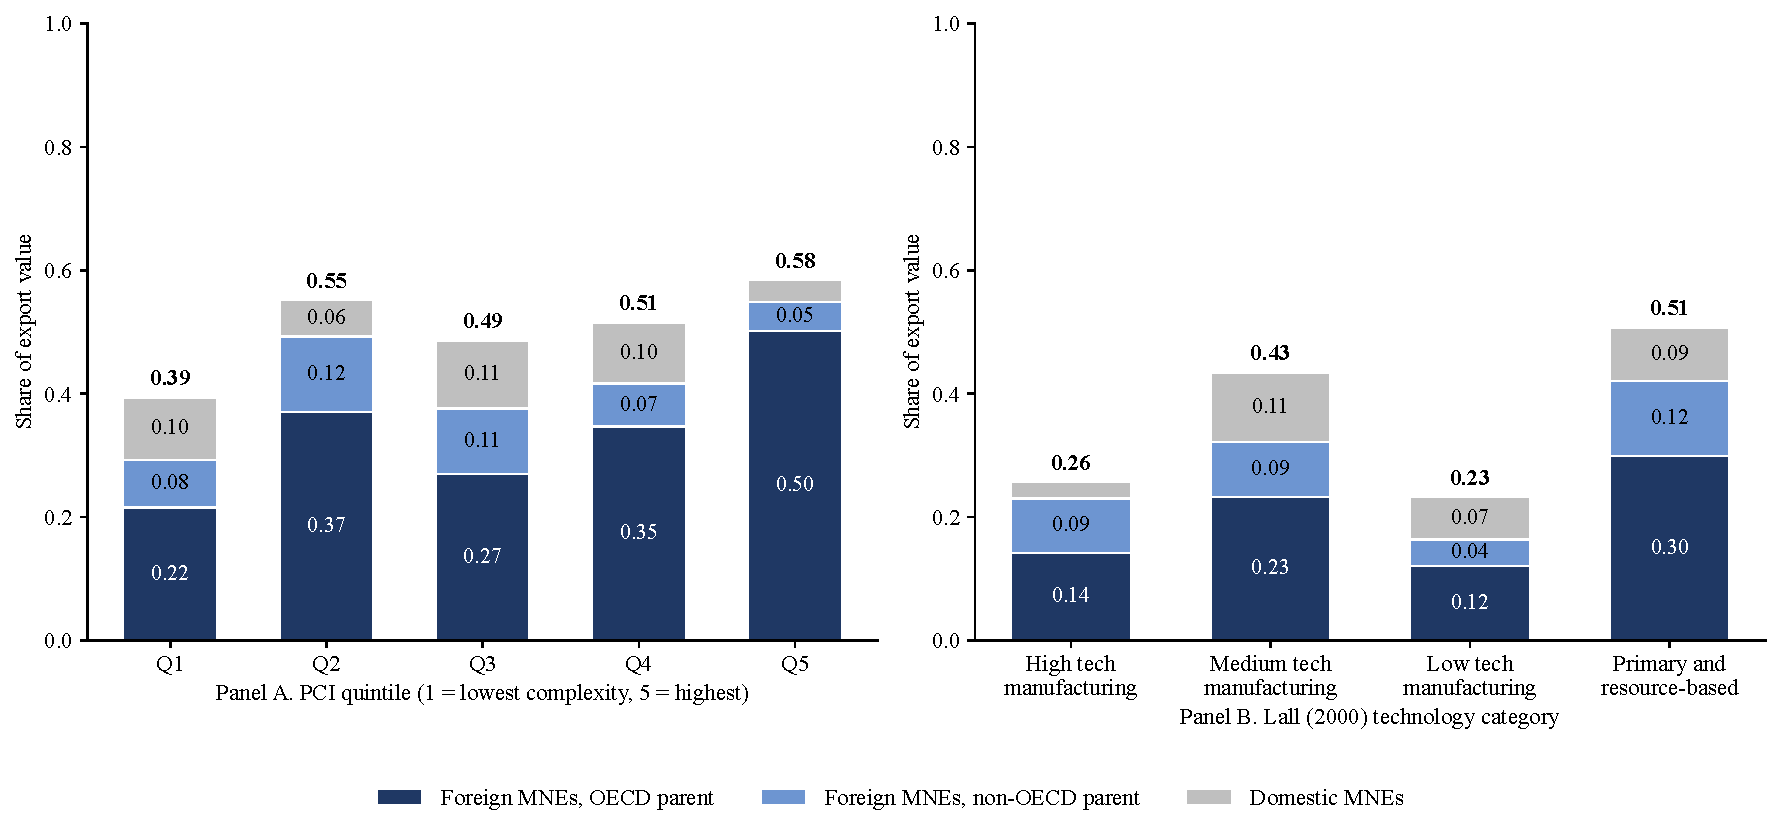
\includegraphics[width=1.0\textwidth,height=0.8\textheight,keepaspectratio]{figures/agro/fig_wp1a_pci_lall_by_oecd.pdf}%
  \caption{Agriculture: Multinational Share of Export Value, by Product Sophistication and Location of the Parent}%
  \label{fig:oecd_agro}%
  \par\vspace{2pt}%
  \parbox{0.92\textwidth}{\footnotesize %
  \textit{Notes:} Shares of agricultural export value (HS 01--24), all available years pooled. Foreign MNEs are split by whether the ultimate parent is in an OECD member country. Panel A: Quintiles of the Hausmann--Hidalgo Product Complexity Index across HS6 products (Q1 = least complex). Panel B: Lall (2000) technology classes: primary and resource-based products, and low-, medium- and high-technology manufactures.\\[3pt]%
  \textit{Source:} Authors' calculations based on customs data matched to Orbis and Dun \& Bradstreet.}%
  \end{figure}

\subsection{Other Measures of Product Sophistication}
% ---- Figure: Agriculture: Multinational Share of Export Value, by Quintile of Six Sophistication Measures
\begin{figure}[H]\centering%
  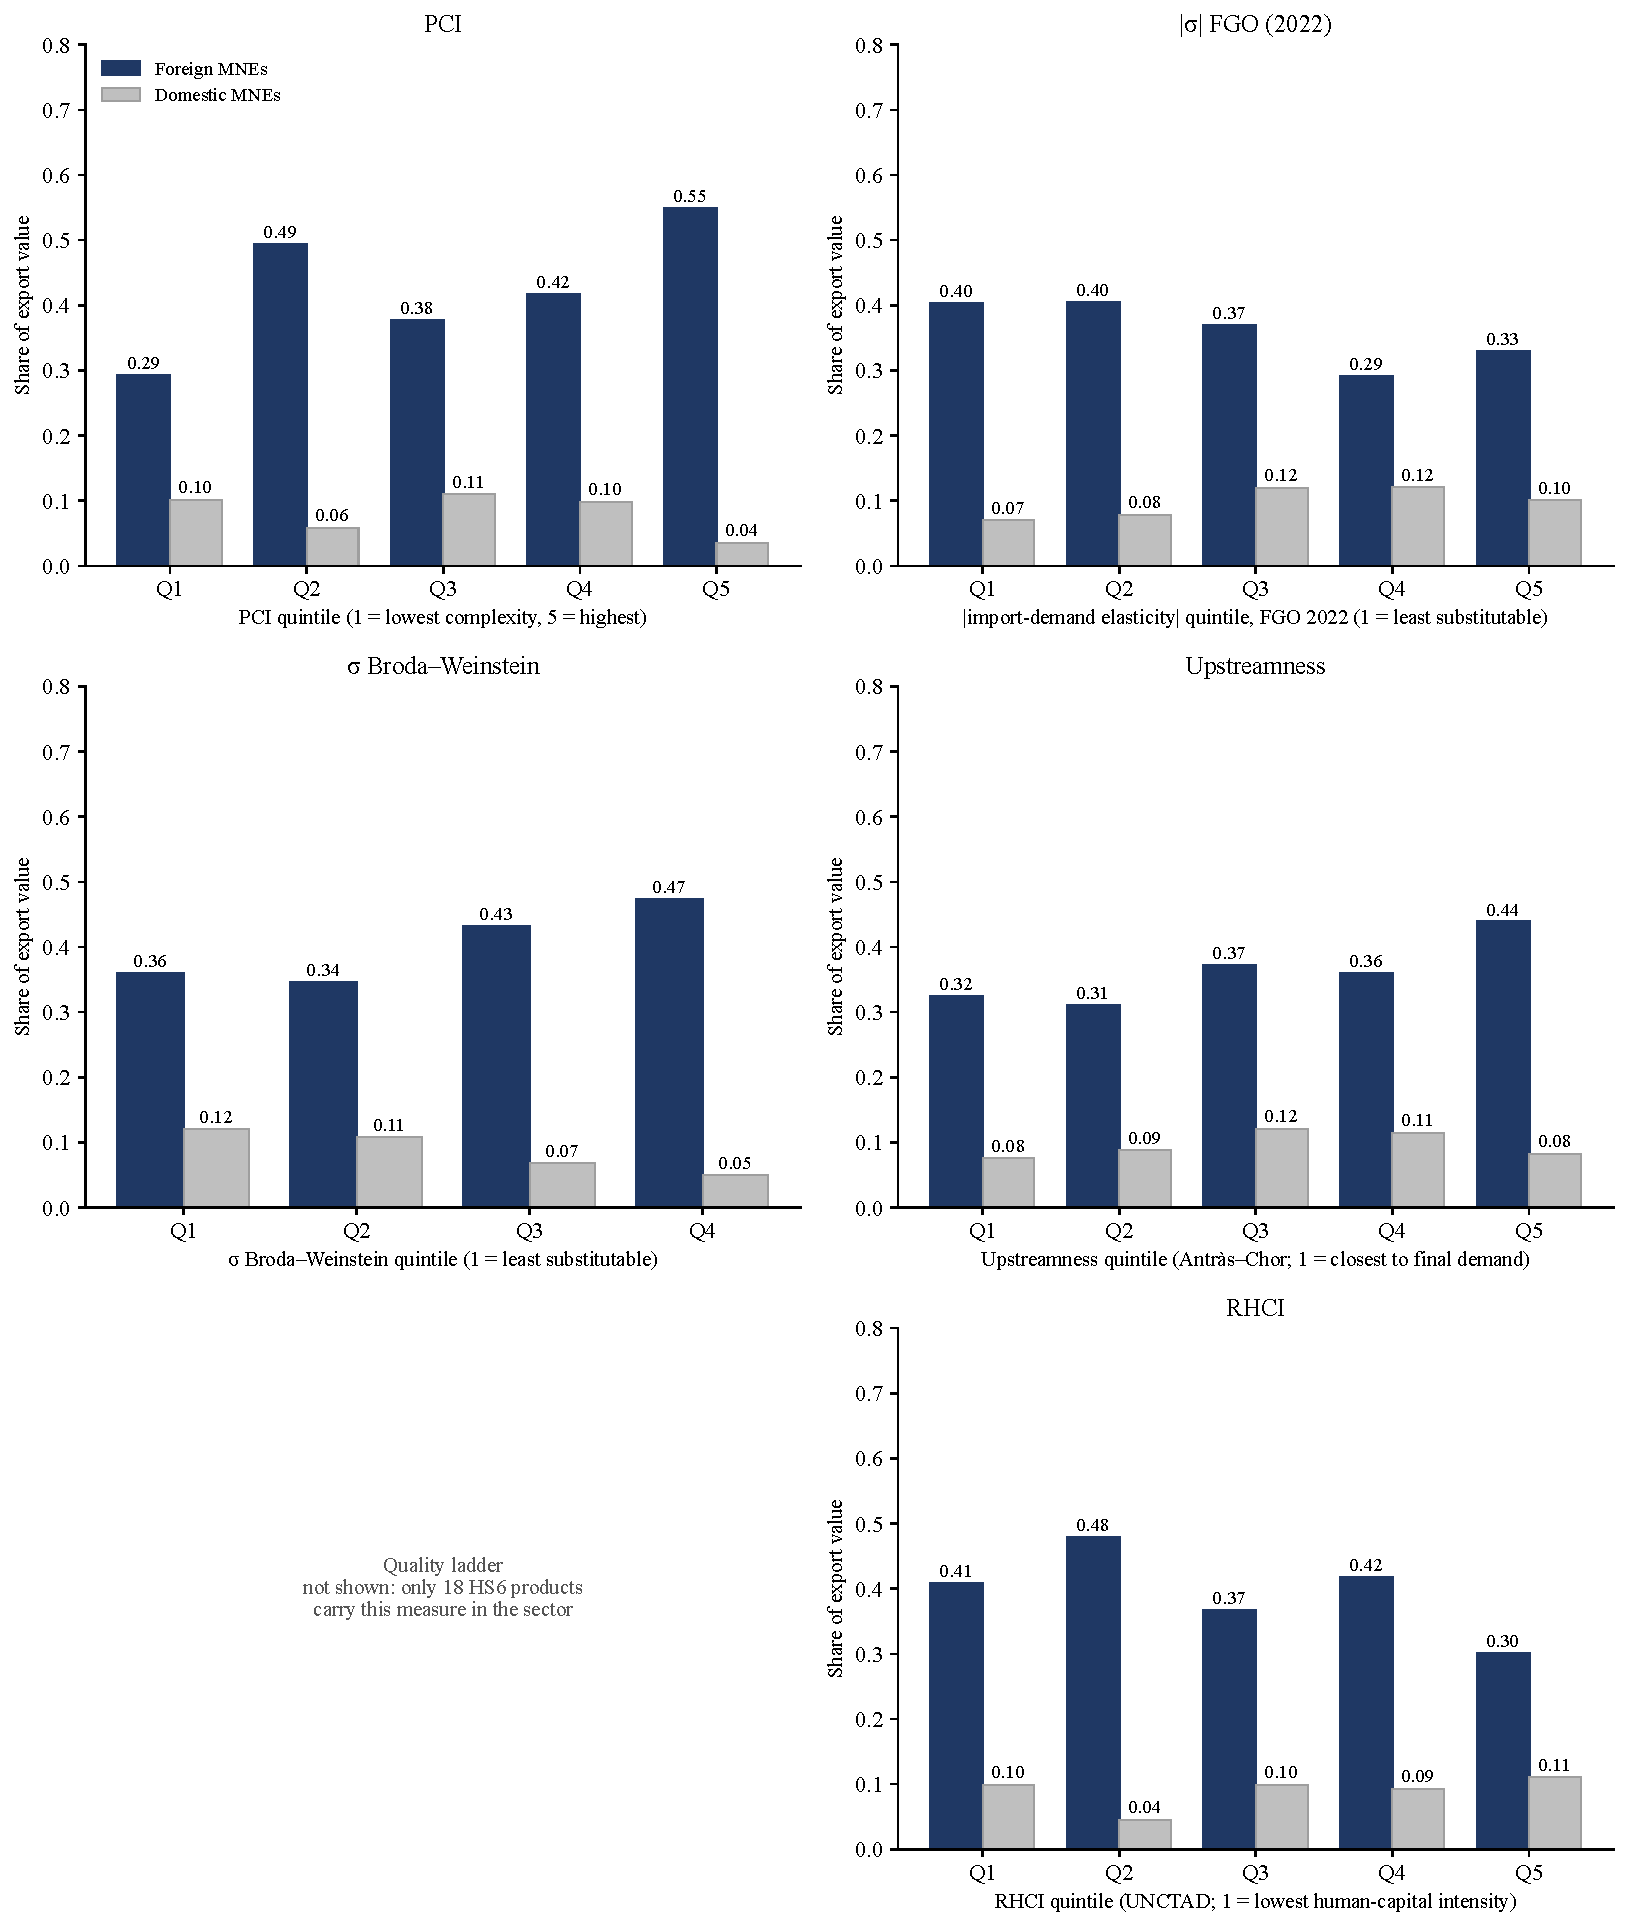
\includegraphics[width=1.0\textwidth,height=0.8\textheight,keepaspectratio]{figures/agro/fig_wp1b_panel_quintiles.pdf}%
  \caption{Agriculture: Multinational Share of Export Value, by Quintile of Six Sophistication Measures}%
  \label{fig:six_q_agro}%
  \par\vspace{2pt}%
  \parbox{0.92\textwidth}{\footnotesize %
  \textit{Notes:} Shares of agricultural export value (HS 01--24), all available years pooled. Quintiles computed over HS6 products. The six measures are the Product Complexity Index, the absolute import-demand elasticity of Fontagn\'e, Guimbard and Orefice (2022), the elasticity of substitution of Broda and Weinstein, upstreamness, the quality ladder and the revealed human-capital intensity of UNCTAD.\\[3pt]%
  \textit{Source:} Authors' calculations based on customs data matched to Orbis and Dun \& Bradstreet.}%
  \end{figure}
% ---- Figure: Agriculture: Multinational Share of Export Value, by Quintile of the Import-Demand Elasticity
\begin{figure}[H]\centering%
  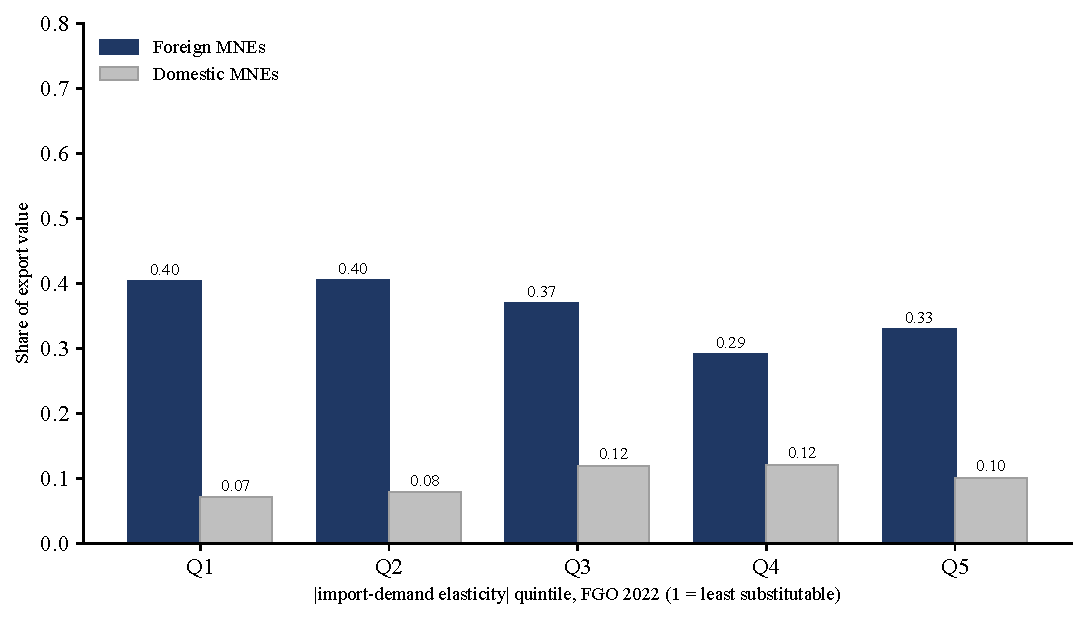
\includegraphics[width=0.78\textwidth,height=0.8\textheight,keepaspectratio]{figures/agro/fig_wp1b_sigma_fgo_abs_quintile.pdf}%
  \caption{Agriculture: Multinational Share of Export Value, by Quintile of the Import-Demand Elasticity}%
  \label{fig:fgo_q_agro}%
  \par\vspace{2pt}%
  \parbox{0.92\textwidth}{\footnotesize %
  \textit{Notes:} Shares of agricultural export value (HS 01--24), all available years pooled. Quintiles of the absolute import-demand elasticity of Fontagn\'e, Guimbard and Orefice (2022) across HS6 products; higher quintiles are more substitutable products.\\[3pt]%
  \textit{Source:} Authors' calculations based on customs data matched to Orbis and Dun \& Bradstreet.}%
  \end{figure}
% ---- Figure: Agriculture: Distribution of Export Value across Six Sophistication Measures
\begin{figure}[H]\centering%
  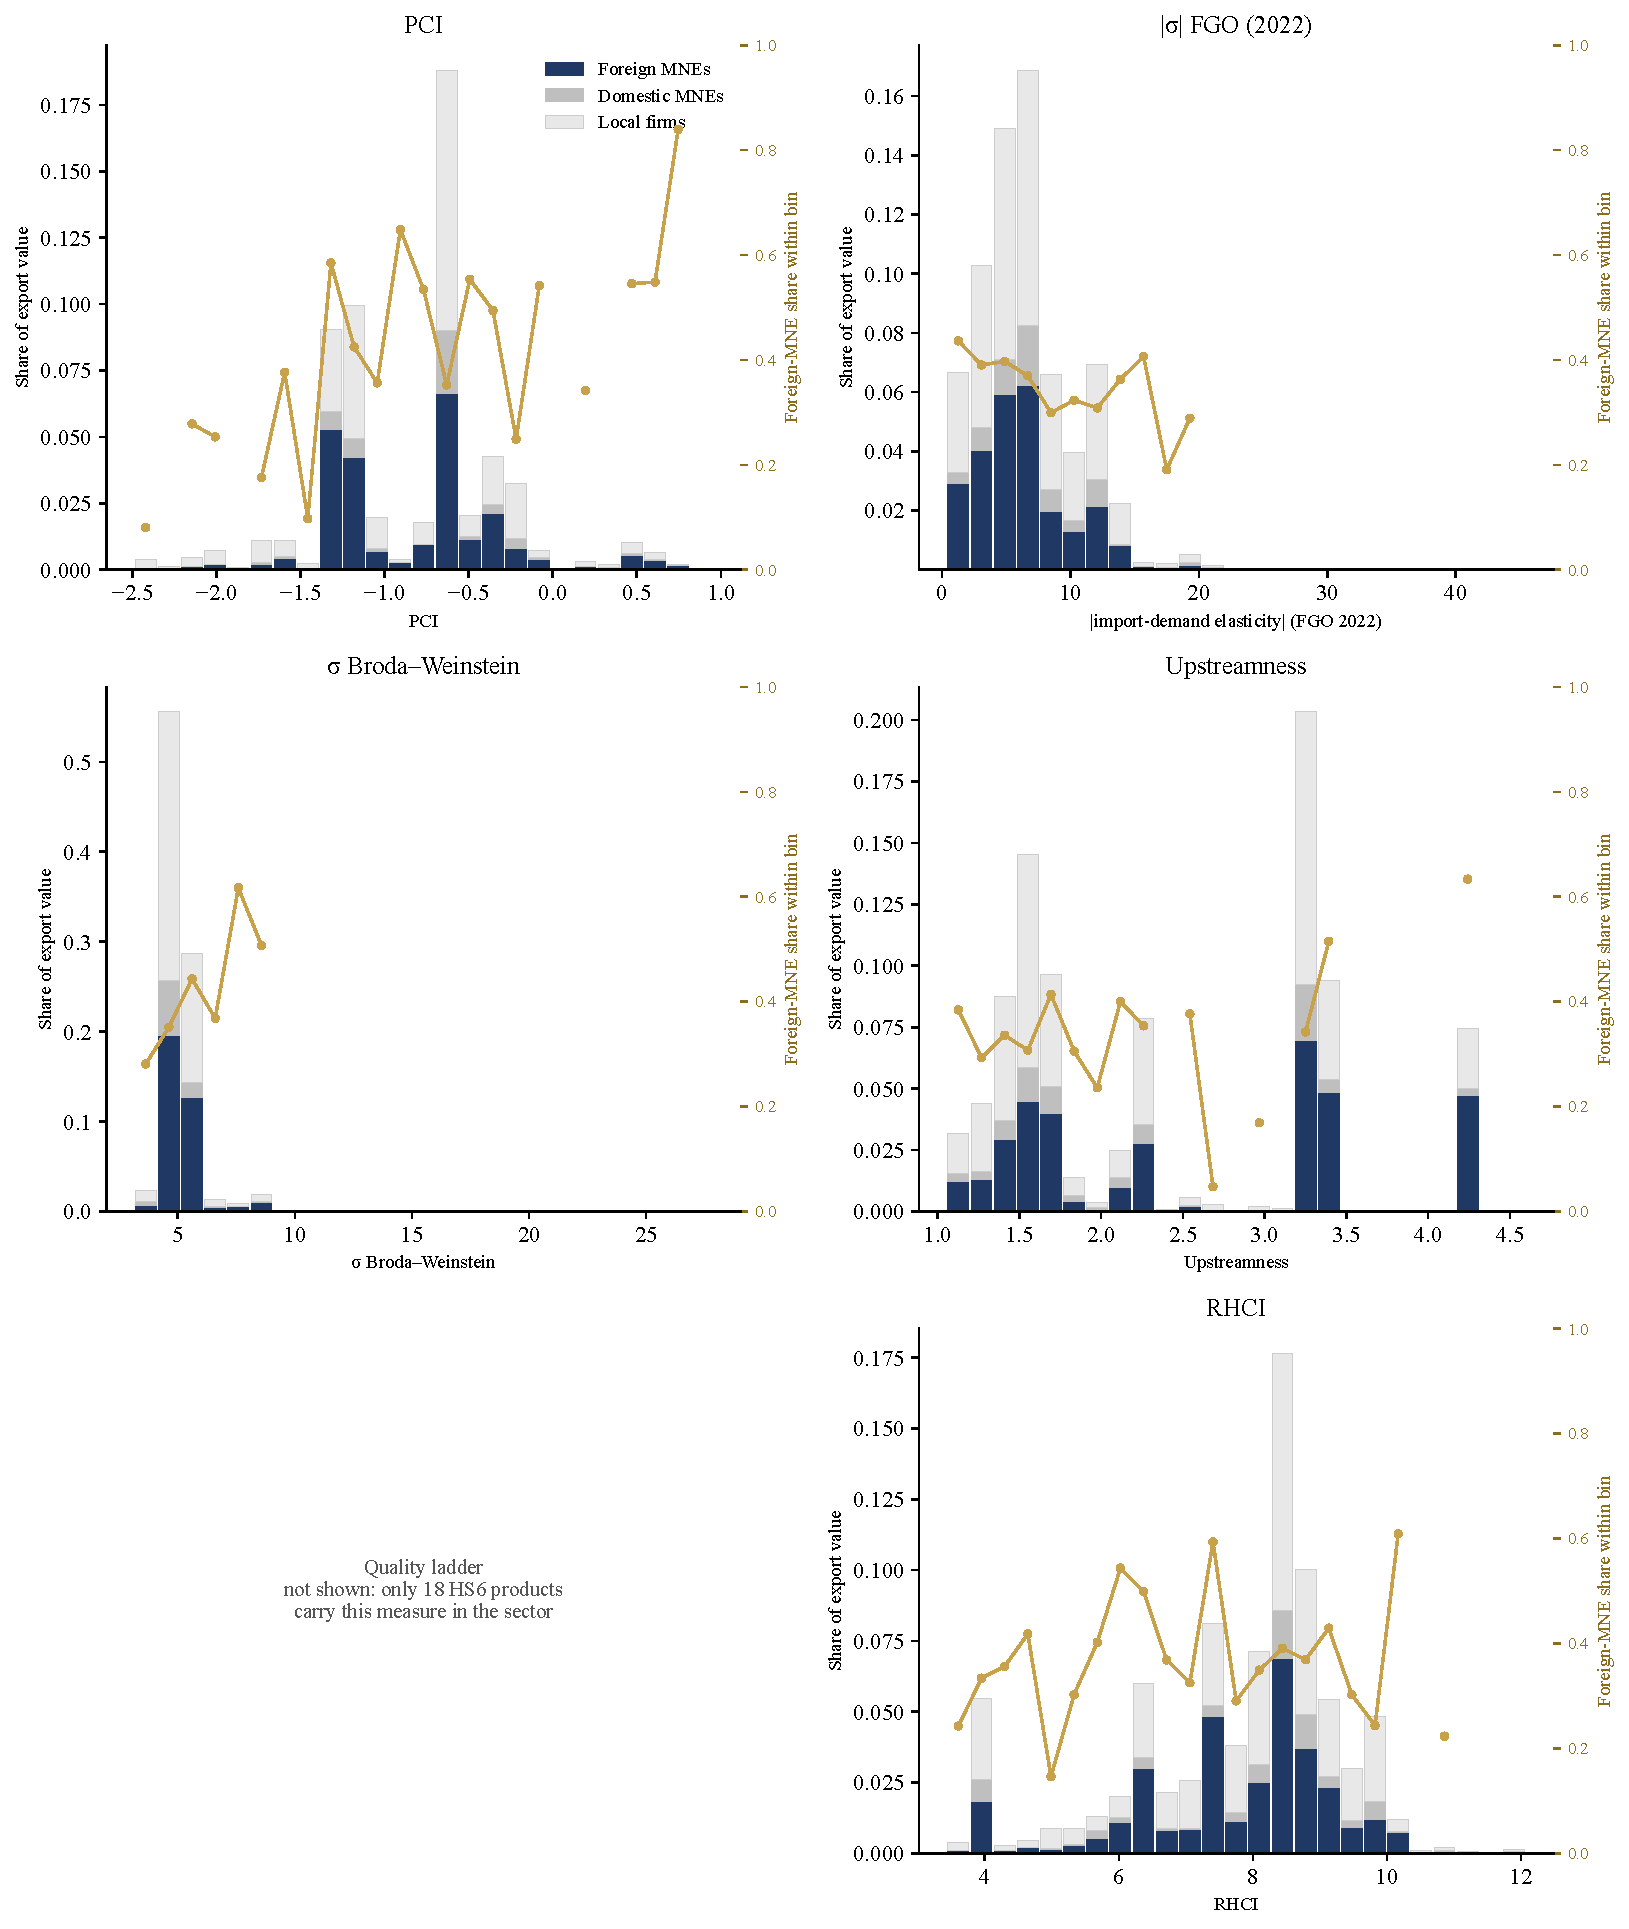
\includegraphics[width=1.0\textwidth,height=0.8\textheight,keepaspectratio]{figures/agro/fig_wp1b_panel_hist.pdf}%
  \caption{Agriculture: Distribution of Export Value across Six Sophistication Measures}%
  \label{fig:six_h_agro}%
  \par\vspace{2pt}%
  \parbox{0.92\textwidth}{\footnotesize %
  \textit{Notes:} Bars: agricultural export value (HS 01--24) in each bin, by type of exporter. Line (right axis): foreign-MNE share of each bin. The six measures are the Product Complexity Index, the absolute import-demand elasticity of Fontagn\'e, Guimbard and Orefice (2022), the elasticity of substitution of Broda and Weinstein, upstreamness, the quality ladder and the revealed human-capital intensity of UNCTAD.\\[3pt]%
  \textit{Source:} Authors' calculations based on customs data matched to Orbis and Dun \& Bradstreet.}%
  \end{figure}
% ---- Figure: Agriculture: Distribution of Export Value across the Import-Demand Elasticity
\begin{figure}[H]\centering%
  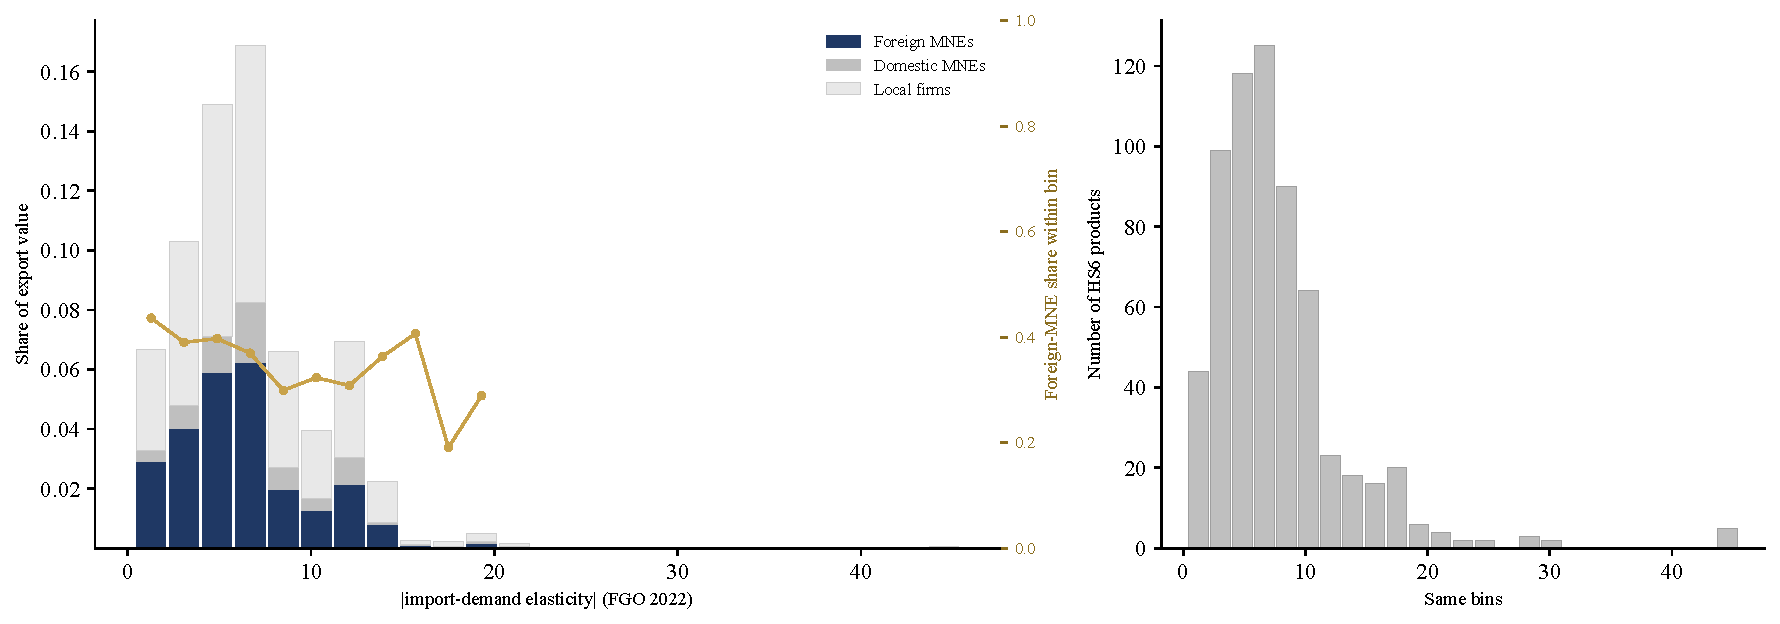
\includegraphics[width=1.0\textwidth,height=0.8\textheight,keepaspectratio]{figures/agro/fig_wp1b_hist_sigma_fgo_abs.pdf}%
  \caption{Agriculture: Distribution of Export Value across the Import-Demand Elasticity}%
  \label{fig:fgo_h_agro}%
  \par\vspace{2pt}%
  \parbox{0.92\textwidth}{\footnotesize %
  \textit{Notes:} Left: export value in each bin, by type of exporter, and the foreign-MNE share of each bin. Right: number of HS6 products in each bin.\\[3pt]%
  \textit{Source:} Authors' calculations based on customs data matched to Orbis and Dun \& Bradstreet.}%
  \end{figure}
% ---- Figure: Agriculture: Distribution of Export Value across the Product Complexity Index
\begin{figure}[H]\centering%
  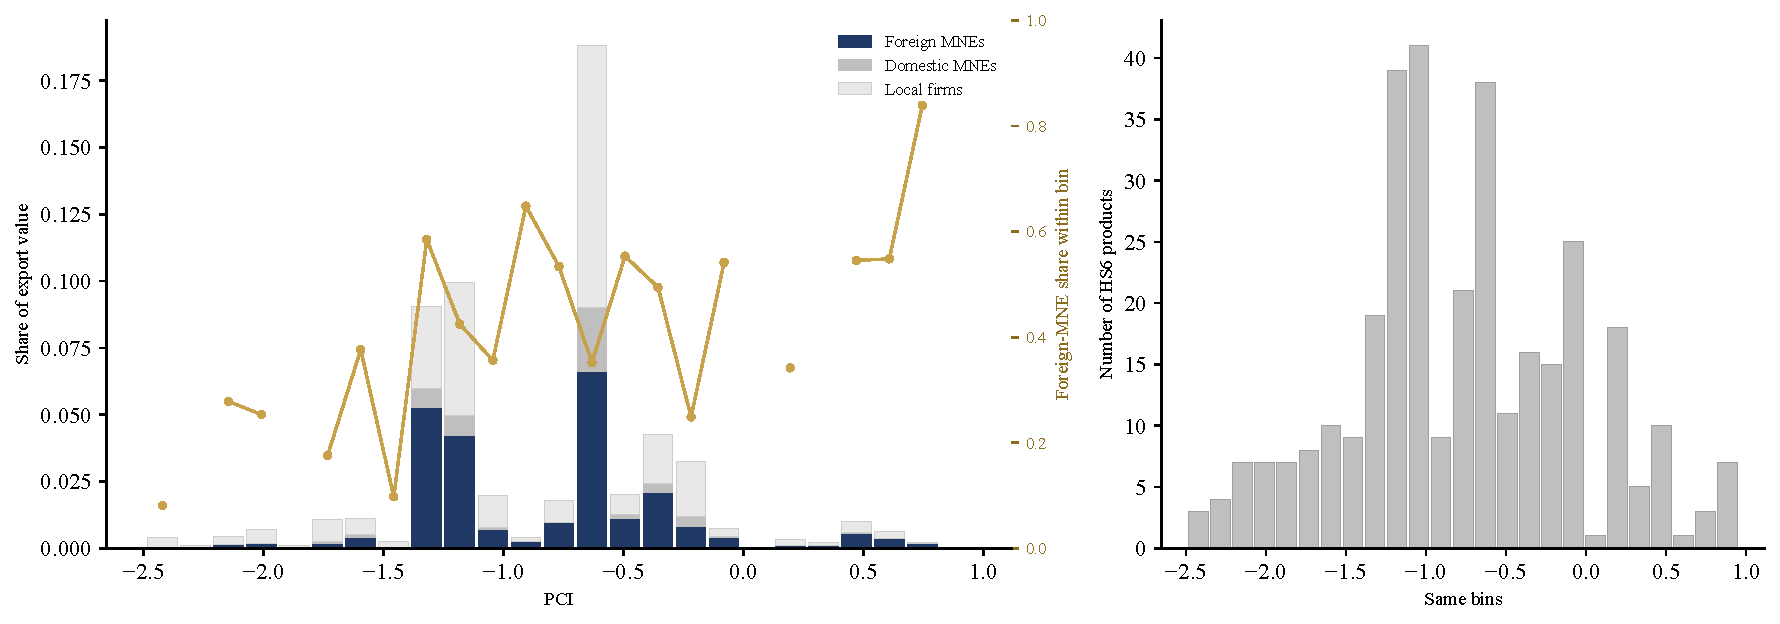
\includegraphics[width=1.0\textwidth,height=0.8\textheight,keepaspectratio]{figures/agro/fig_wp1b_hist_complexity.pdf}%
  \caption{Agriculture: Distribution of Export Value across the Product Complexity Index}%
  \label{fig:pci_h_agro}%
  \par\vspace{2pt}%
  \parbox{0.92\textwidth}{\footnotesize %
  \textit{Notes:} Left: export value in each bin, by type of exporter, and the foreign-MNE share of each bin. Right: number of HS6 products in each bin.\\[3pt]%
  \textit{Source:} Authors' calculations based on customs data matched to Orbis and Dun \& Bradstreet.}%
  \end{figure}
% ---- Table: Agriculture: Multinational Share of Export Value, by Quintile of Six Sophistication Measures
\begin{table}[H]\centering\small%
  \caption{Agriculture: Multinational Share of Export Value, by Quintile of Six Sophistication Measures}%
  \label{tab:six_t_agro}%
  \adjustbox{max width=\textwidth, max totalheight=0.8\textheight}{\begin{tabular}{lccccc|ccccc}
\toprule
 & \multicolumn{5}{c}{Foreign MNE share} & \multicolumn{5}{c}{Domestic MNE share} \\
Measure & Q1 & Q2 & Q3 & Q4 & Q5 & Q1 & Q2 & Q3 & Q4 & Q5 \\
\midrule
PCI & 0.29 & 0.49 & 0.38 & 0.42 & 0.55 & 0.10 & 0.06 & 0.11 & 0.10 & 0.04 \\
$|\sigma|$ FGO (2022) & 0.40 & 0.40 & 0.37 & 0.29 & 0.33 & 0.07 & 0.08 & 0.12 & 0.12 & 0.10 \\
$\sigma$ Broda--Weinstein & 0.36 & 0.34 & 0.43 & 0.47 & -- & 0.12 & 0.11 & 0.07 & 0.05 & -- \\
Upstreamness & 0.32 & 0.31 & 0.37 & 0.36 & 0.44 & 0.08 & 0.09 & 0.12 & 0.11 & 0.08 \\
Quality ladder & -- & -- & -- & -- & -- & -- & -- & -- & -- & -- \\
RHCI & 0.41 & 0.48 & 0.37 & 0.42 & 0.30 & 0.10 & 0.04 & 0.10 & 0.09 & 0.11 \\
\bottomrule
\end{tabular}
}%
  \par\vspace{3pt}%
  \begin{minipage}{0.95\textwidth}\footnotesize %
  \textit{Notes:} Shares of agricultural export value (HS 01--24), all available years pooled. Quintiles computed over HS6 products. --: fewer than 30 HS6 products carry the measure.\\[3pt]%
  \textit{Source:} Authors' calculations based on customs data matched to Orbis and Dun \& Bradstreet.%
  \end{minipage}%
  \end{table}
% ---- Table: Agriculture: Correlations between Sophistication Measures
\begin{table}[H]\centering\small%
  \caption{Agriculture: Correlations between Sophistication Measures}%
  \label{tab:corr_agro}%
  \adjustbox{max width=\textwidth, max totalheight=0.8\textheight}{\begin{tabular}{lrrrrrr}
\toprule
 & PCI & $|\sigma|$ FGO (2022) & $\sigma$ Broda--Weinstein & Upstreamness & Quality ladder & RHCI \\
\midrule
PCI & 1.00 & -0.12 & -0.16 & -0.21 & -- & 0.72 \\
$|\sigma|$ FGO (2022) & -0.12 & 1.00 & 0.01 & 0.13 & -- & 0.03 \\
$\sigma$ Broda--Weinstein & -0.16 & 0.01 & 1.00 & 0.08 & -- & -0.09 \\
Upstreamness & -0.21 & 0.13 & 0.08 & 1.00 & -- & 0.01 \\
Quality ladder & -- & -- & -- & -- & -- & -- \\
RHCI & 0.72 & 0.03 & -0.09 & 0.01 & -- & 1.00 \\
\bottomrule
\end{tabular}
}%
  \par\vspace{3pt}%
  \begin{minipage}{0.95\textwidth}\footnotesize %
  \textit{Notes:} Correlations across HS6 products, weighted by export value.\\[3pt]%
  \textit{Source:} Authors' calculations based on customs data matched to Orbis and Dun \& Bradstreet.%
  \end{minipage}%
  \end{table}

\subsection{Rauch Classes and End Use}
% ---- Table: Agriculture: Multinational Share of Export Value, by Rauch Product Class
\begin{table}[H]\centering\small%
  \caption{Agriculture: Multinational Share of Export Value, by Rauch Product Class}%
  \label{tab:rauch_agro}%
  \adjustbox{max width=\textwidth, max totalheight=0.8\textheight}{\begin{tabular}{lcccrr}
\toprule
Rauch (1999) class & Foreign & Domestic & All MNEs & HS6 products & Value (US\$bn/yr) \\
\midrule
Differentiated & 0.413 & 0.093 & 0.506 & 167 & 7.8 \\
Reference-priced & 0.315 & 0.098 & 0.413 & 357 & 20.1 \\
Homogeneous (exchange) & 0.409 & 0.094 & 0.503 & 164 & 43.7 \\
\bottomrule
\end{tabular}
}%
  \par\vspace{3pt}%
  \begin{minipage}{0.95\textwidth}\footnotesize %
  \textit{Notes:} Shares of agricultural export value (HS 01--24), all available years pooled. Rauch (1999) conservative classification: homogeneous goods are traded on organized exchanges, reference-priced goods have a price quoted in trade publications, and differentiated goods have neither. Values are annual averages in US\$ billion.\\[3pt]%
  \textit{Source:} Authors' calculations based on customs data matched to Orbis and Dun \& Bradstreet.%
  \end{minipage}%
  \end{table}
% ---- Figure: Agriculture: Multinational Share of Export Value, by Rauch Product Class
\begin{figure}[H]\centering%
  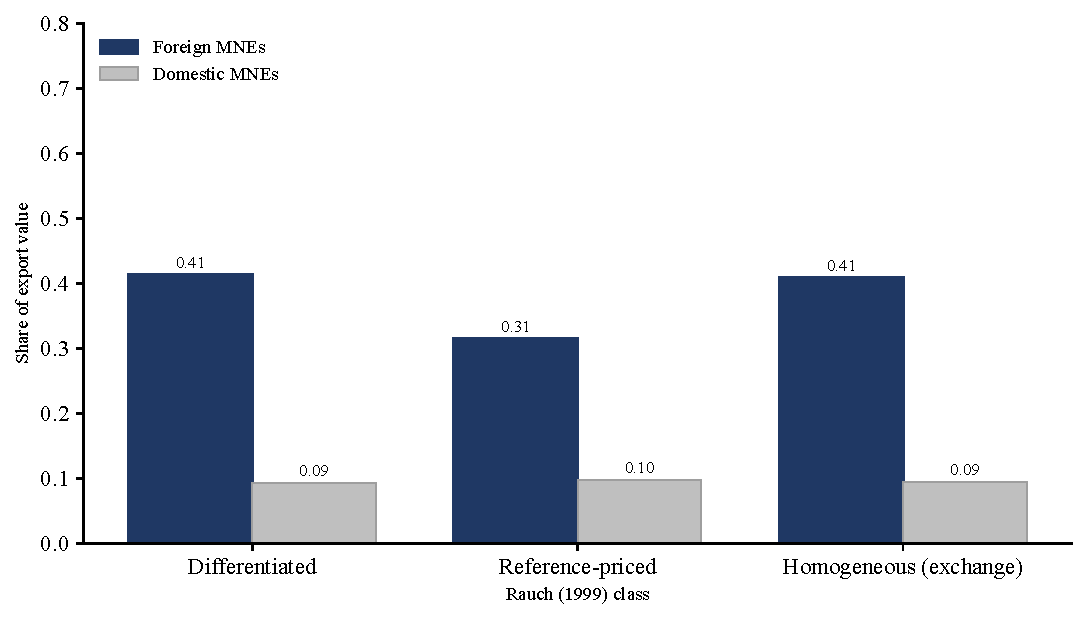
\includegraphics[width=0.7\textwidth,height=0.8\textheight,keepaspectratio]{figures/agro/fig_wp1b_rauch.pdf}%
  \caption{Agriculture: Multinational Share of Export Value, by Rauch Product Class}%
  \label{fig:rauch_f_agro}%
  \par\vspace{2pt}%
  \parbox{0.92\textwidth}{\footnotesize %
  \textit{Notes:} Shares of agricultural export value (HS 01--24), all available years pooled. Rauch (1999) conservative classification: homogeneous goods are traded on organized exchanges, reference-priced goods have a price quoted in trade publications, and differentiated goods have neither.\\[3pt]%
  \textit{Source:} Authors' calculations based on customs data matched to Orbis and Dun \& Bradstreet.}%
  \end{figure}
% ---- Table: Agriculture: Multinational Share of Export Value: Differentiated and Other Products
\begin{table}[H]\centering\small%
  \caption{Agriculture: Multinational Share of Export Value: Differentiated and Other Products}%
  \label{tab:rauch2_agro}%
  \adjustbox{max width=\textwidth, max totalheight=0.8\textheight}{\begin{tabular}{lcccrr}
\toprule
Rauch (1999): differentiated vs non-differentiated & Foreign & Domestic & All MNEs & HS6 products & Value (US\$bn/yr) \\
\midrule
Differentiated & 0.413 & 0.093 & 0.506 & 167 & 7.8 \\
Non-differentiated & 0.377 & 0.096 & 0.473 & 521 & 63.8 \\
\bottomrule
\end{tabular}
}%
  \par\vspace{3pt}%
  \begin{minipage}{0.95\textwidth}\footnotesize %
  \textit{Notes:} Shares of agricultural export value (HS 01--24), all available years pooled. Rauch (1999) conservative classification; other products are reference-priced and homogeneous goods. Values are annual averages in US\$ billion.\\[3pt]%
  \textit{Source:} Authors' calculations based on customs data matched to Orbis and Dun \& Bradstreet.%
  \end{minipage}%
  \end{table}
% ---- Figure: Agriculture: Multinational Share of Export Value: Differentiated and Other Products
\begin{figure}[H]\centering%
  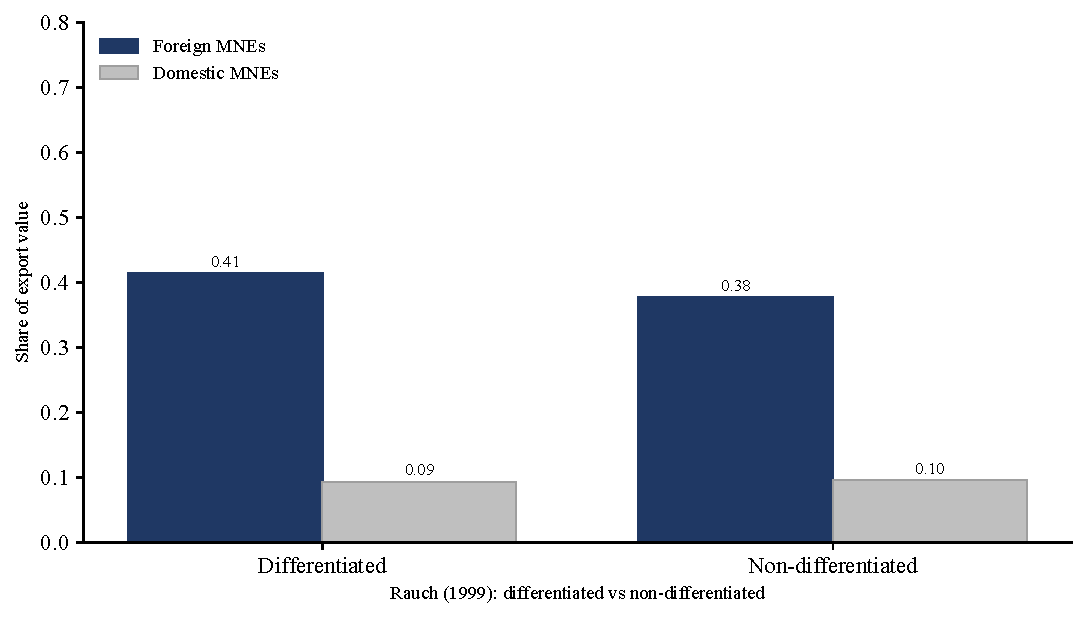
\includegraphics[width=0.7\textwidth,height=0.8\textheight,keepaspectratio]{figures/agro/fig_wp1b_rauch2.pdf}%
  \caption{Agriculture: Multinational Share of Export Value: Differentiated and Other Products}%
  \label{fig:rauch2_f_agro}%
  \par\vspace{2pt}%
  \parbox{0.92\textwidth}{\footnotesize %
  \textit{Notes:} Shares of agricultural export value (HS 01--24), all available years pooled. Rauch (1999) conservative classification; other products are reference-priced and homogeneous goods.\\[3pt]%
  \textit{Source:} Authors' calculations based on customs data matched to Orbis and Dun \& Bradstreet.}%
  \end{figure}
% ---- Table: Agriculture: Multinational Share of Export Value, by End Use
\begin{table}[H]\centering\small%
  \caption{Agriculture: Multinational Share of Export Value, by End Use}%
  \label{tab:bec_agro}%
  \adjustbox{max width=\textwidth, max totalheight=0.8\textheight}{\begin{tabular}{lcccrr}
\toprule
BEC end use & Foreign & Domestic & All MNEs & HS6 products & Value (US\$bn/yr) \\
\midrule
Intermediate & 0.411 & 0.090 & 0.501 & 243 & 42.5 \\
Consumption & 0.351 & 0.099 & 0.450 & 456 & 30.4 \\
Capital & 0.168 & 0.020 & 0.187 & 3 & 0.0 \\
\bottomrule
\end{tabular}
}%
  \par\vspace{3pt}%
  \begin{minipage}{0.95\textwidth}\footnotesize %
  \textit{Notes:} Shares of agricultural export value (HS 01--24), all available years pooled. End use from BEC Rev.\,4; HS6 products without a BEC correspondence are excluded. Values are annual averages in US\$ billion.\\[3pt]%
  \textit{Source:} Authors' calculations based on customs data matched to Orbis and Dun \& Bradstreet.%
  \end{minipage}%
  \end{table}

\subsection{Regressions}
% ---- Table: Agriculture: Product Characteristics and Multinational Shares
\begin{table}[H]\centering\small%
  \caption{Agriculture: Product Characteristics and Multinational Shares}%
  \label{tab:fgo_r_agro}%
  \adjustbox{max width=\textwidth, max totalheight=0.8\textheight}{\begin{tabular}{lccc} \hline
 & (1) & (2) & (3) \\ \hline
\multicolumn{4}{l}{\textit{Panel A. Dependent variable: share of all MNEs}} \\
Complexity (PCI) & 0.0838*** & 0.0831*** & 0.0763*** \\
 & (0.0067) & (0.0065) & (0.0067) \\
$|\sigma|$ FGO (per s.d.) & -0.0225*** & -0.0231*** & -0.0268*** \\
 & (0.0038) & (0.0036) & (0.0036) \\
Upstreamness & 0.0129** & 0.0112** & 0.0086 \\
 & (0.0055) & (0.0052) & (0.0053) \\
\midrule
\multicolumn{4}{l}{\textit{Panel B. Dependent variable: share of foreign MNEs}} \\
Complexity (PCI) & 0.0757*** & 0.0771*** & 0.0737*** \\
 & (0.0070) & (0.0069) & (0.0071) \\
$|\sigma|$ FGO (per s.d.) & -0.0499*** & -0.0499*** & -0.0539*** \\
 & (0.0037) & (0.0035) & (0.0035) \\
Upstreamness & 0.0241*** & 0.0230*** & 0.0141*** \\
 & (0.0055) & (0.0053) & (0.0054) \\
\midrule
\multicolumn{4}{l}{\textit{Panel C. Dependent variable: share of domestic MNEs}} \\
Complexity (PCI) & 0.0081** & 0.0061 & 0.0026 \\
 & (0.0039) & (0.0038) & (0.0038) \\
$|\sigma|$ FGO (per s.d.) & 0.0273*** & 0.0268*** & 0.0271*** \\
 & (0.0020) & (0.0018) & (0.0018) \\
Upstreamness & -0.0112*** & -0.0118*** & -0.0055** \\
 & (0.0027) & (0.0026) & (0.0023) \\
\hline
Origin FE & $\checkmark$ &  &  \\
Destination FE & $\checkmark$ &  &  \\
Year FE & $\checkmark$ &  &  \\
Origin $\times$ year FE &  & $\checkmark$ &  \\
Destination $\times$ year FE &  & $\checkmark$ &  \\
Origin $\times$ dest.\ $\times$ year FE &  &  & $\checkmark$ \\
Observations & 150,776 & 150,391 & 148,224 \\
\hline
\end{tabular}
}%
  \par\vspace{3pt}%
  \begin{minipage}{0.95\textwidth}\footnotesize %
  \textit{Notes:} Observations are origin--destination--HS6--year cells. Agriculture products only. Dependent variable: share of the cell's export value shipped by each type of MNE. The import-demand elasticity is standardized (mean 0, standard deviation 1). Regressions weighted by the cell's export value. Robust standard errors in parentheses. *** $p<0.01$, ** $p<0.05$, * $p<0.1$.\\[3pt]%
  \textit{Source:} Authors' calculations based on customs data matched to Orbis and Dun \& Bradstreet.%
  \end{minipage}%
  \end{table}
% ---- Table: Agriculture: Product Sophistication and Multinational Shares
\begin{table}[H]\centering\footnotesize%
  \caption{Agriculture: Product Sophistication and Multinational Shares}%
  \label{tab:meas_r_agro}%
  \adjustbox{max width=\textwidth, max totalheight=0.8\textheight}{\begin{tabular}{lcccccc} \hline
 & \multicolumn{2}{c}{PCI} & \multicolumn{2}{c}{Lall} & \multicolumn{2}{c}{Rauch} \\
 & (1) & (2) & (3) & (4) & (5) & (6) \\ \hline
\multicolumn{7}{l}{\textit{Panel A. Dependent variable: share of all MNEs}} \\
Complexity (PCI) & 0.0733*** & 0.0614*** &  &  &  &  \\
 & (0.0061) & (0.0064) &  &  &  &  \\
Lall: high tech (vs primary and resource-based) &  &  & -0.2016*** & -0.2103*** &  &  \\
 &  &  & (0.0104) & (0.0102) &  &  \\
Lall: medium tech &  &  & -0.0395*** & -0.0465*** &  &  \\
 &  &  & (0.0060) & (0.0066) &  &  \\
Lall: low tech &  &  & -0.2467*** & -0.2272*** &  &  \\
 &  &  & (0.0278) & (0.0268) &  &  \\
Rauch: differentiated (vs homogeneous) &  &  &  &  & 0.0435*** & 0.0488*** \\
 &  &  &  &  & (0.0088) & (0.0098) \\
Rauch: reference-priced &  &  &  &  & -0.0460*** & -0.0393*** \\
 &  &  &  &  & (0.0068) & (0.0066) \\
Observations & 158,616 & 156,478 & 274,948 & 272,985 & 271,105 & 269,190 \\
\midrule
\multicolumn{7}{l}{\textit{Panel B. Dependent variable: share of foreign MNEs}} \\
Complexity (PCI) & 0.0562*** & 0.0490*** &  &  &  &  \\
 & (0.0067) & (0.0072) &  &  &  &  \\
Lall: high tech (vs primary and resource-based) &  &  & -0.1480*** & -0.1576*** &  &  \\
 &  &  & (0.0091) & (0.0094) &  &  \\
Lall: medium tech &  &  & -0.0623*** & -0.0678*** &  &  \\
 &  &  & (0.0067) & (0.0073) &  &  \\
Lall: low tech &  &  & -0.2301*** & -0.2262*** &  &  \\
 &  &  & (0.0153) & (0.0139) &  &  \\
Rauch: differentiated (vs homogeneous) &  &  &  &  & 0.0554*** & 0.0560*** \\
 &  &  &  &  & (0.0097) & (0.0107) \\
Rauch: reference-priced &  &  &  &  & -0.0439*** & -0.0383*** \\
 &  &  &  &  & (0.0069) & (0.0066) \\
Observations & 158,616 & 156,478 & 274,948 & 272,985 & 271,105 & 269,190 \\
\midrule
\multicolumn{7}{l}{\textit{Panel C. Dependent variable: share of domestic MNEs}} \\
Complexity (PCI) & 0.0172*** & 0.0123*** &  &  &  &  \\
 & (0.0031) & (0.0033) &  &  &  &  \\
Lall: high tech (vs primary and resource-based) &  &  & -0.0536*** & -0.0527*** &  &  \\
 &  &  & (0.0051) & (0.0053) &  &  \\
Lall: medium tech &  &  & 0.0229*** & 0.0212*** &  &  \\
 &  &  & (0.0032) & (0.0033) &  &  \\
Lall: low tech &  &  & -0.0165 & -0.0010 &  &  \\
 &  &  & (0.0247) & (0.0273) &  &  \\
Rauch: differentiated (vs homogeneous) &  &  &  &  & -0.0120*** & -0.0071* \\
 &  &  &  &  & (0.0044) & (0.0043) \\
Rauch: reference-priced &  &  &  &  & -0.0021 & -0.0010 \\
 &  &  &  &  & (0.0038) & (0.0040) \\
Observations & 158,616 & 156,478 & 274,948 & 272,985 & 271,105 & 269,190 \\
\hline
Origin $\times$ year and destination $\times$ year FE & $\checkmark$ &  & $\checkmark$ &  & $\checkmark$ &  \\
Origin $\times$ dest.\ $\times$ year FE &  & $\checkmark$ &  & $\checkmark$ &  & $\checkmark$ \\
\hline
\end{tabular}
}%
  \par\vspace{3pt}%
  \begin{minipage}{0.95\textwidth}\footnotesize %
  \textit{Notes:} Observations are origin--destination--HS6--year cells. Agriculture products only. Dependent variable: share of the cell's export value shipped by each type of MNE. Omitted categories: primary and resource-based products (Lall) and homogeneous products (Rauch). Robust standard errors in parentheses. *** $p<0.01$, ** $p<0.05$, * $p<0.1$.\\[3pt]%
  \textit{Source:} Authors' calculations based on customs data matched to Orbis and Dun \& Bradstreet.%
  \end{minipage}%
  \end{table}

\section{Fact 3: Multinationals from a Small Set of Countries Dominate Exports}\label{sec:f3_agro}

\subsection{Parent Countries}
% ---- Figure: Agriculture: Foreign-Multinational Exports, by Parent Country
\begin{figure}[H]\centering%
  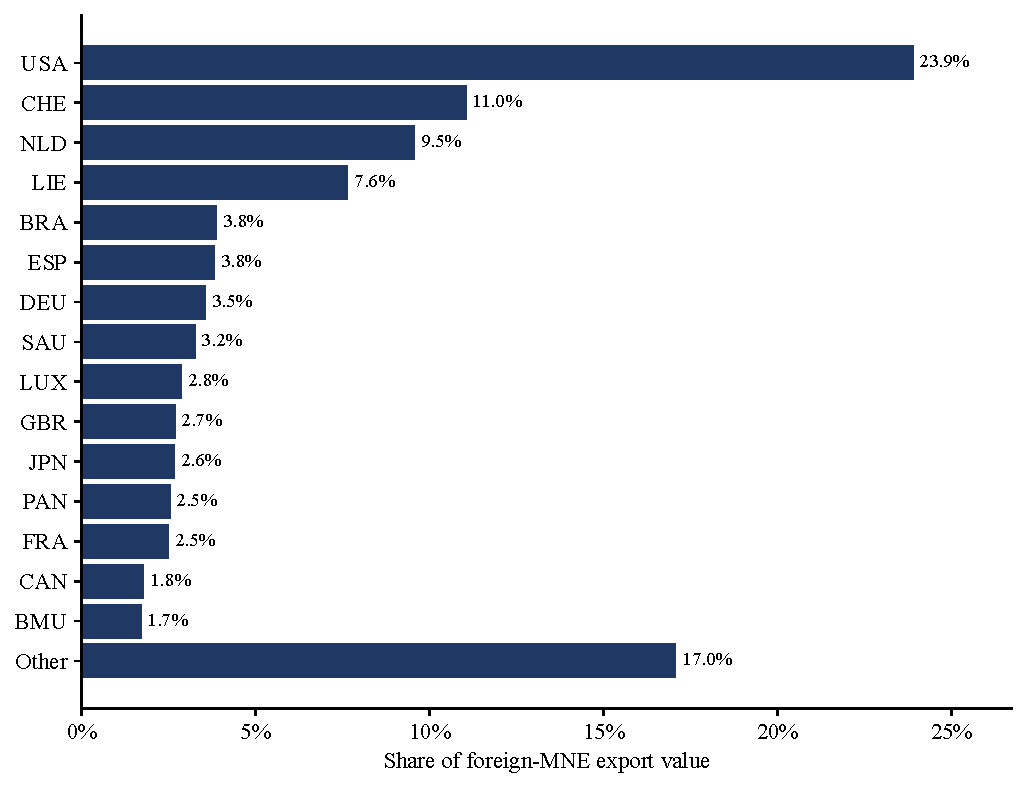
\includegraphics[width=0.78\textwidth,height=0.8\textheight,keepaspectratio]{figures/agro/fig_wp1a_parent_share.pdf}%
  \caption{Agriculture: Foreign-Multinational Exports, by Parent Country}%
  \label{fig:f4_agro}%
  \par\vspace{2pt}%
  \parbox{0.92\textwidth}{\footnotesize %
  \textit{Notes:} Percent of foreign-MNE agricultural export value, by country of the ultimate parent.\\[3pt]%
  \textit{Source:} Authors' calculations based on customs data matched to Orbis and Dun \& Bradstreet.}%
  \end{figure}
% ---- Table: Agriculture: Foreign-Multinational Exports, by Parent Country
\begin{table}[H]\centering\small%
  \caption{Agriculture: Foreign-Multinational Exports, by Parent Country}%
  \label{tab:f4n_agro}%
  \adjustbox{max width=\textwidth, max totalheight=0.8\textheight}{\begin{tabular}{lrr}
\toprule
Parent country & Share (\%) & Value (US\$bn/yr) \\
\midrule
USA & 23.9 & 6.7 \\
CHE & 11.0 & 3.1 \\
NLD & 9.5 & 2.7 \\
LIE & 7.6 & 2.2 \\
BRA & 3.8 & 1.1 \\
ESP & 3.8 & 1.0 \\
DEU & 3.5 & 0.8 \\
SAU & 3.2 & 0.9 \\
LUX & 2.8 & 0.8 \\
GBR & 2.7 & 0.7 \\
JPN & 2.6 & 0.6 \\
PAN & 2.5 & 0.6 \\
FRA & 2.5 & 0.7 \\
CAN & 1.8 & 0.4 \\
BMU & 1.7 & 0.5 \\
Other (115 countries) & 17.0 & 4.4 \\
\midrule
All foreign MNEs & 100.0 & 30.7 \\
\bottomrule
\end{tabular}
}%
  \par\vspace{3pt}%
  \begin{minipage}{0.95\textwidth}\footnotesize %
  \textit{Notes:} Percent of foreign-MNE agricultural export value, by country of the ultimate parent. Values are annual averages in US\$ billion.\\[3pt]%
  \textit{Source:} Authors' calculations based on customs data matched to Orbis and Dun \& Bradstreet.%
  \end{minipage}%
  \end{table}
% ---- Figure: Agriculture: Share of Total Exports, by Parent Country
\begin{figure}[H]\centering%
  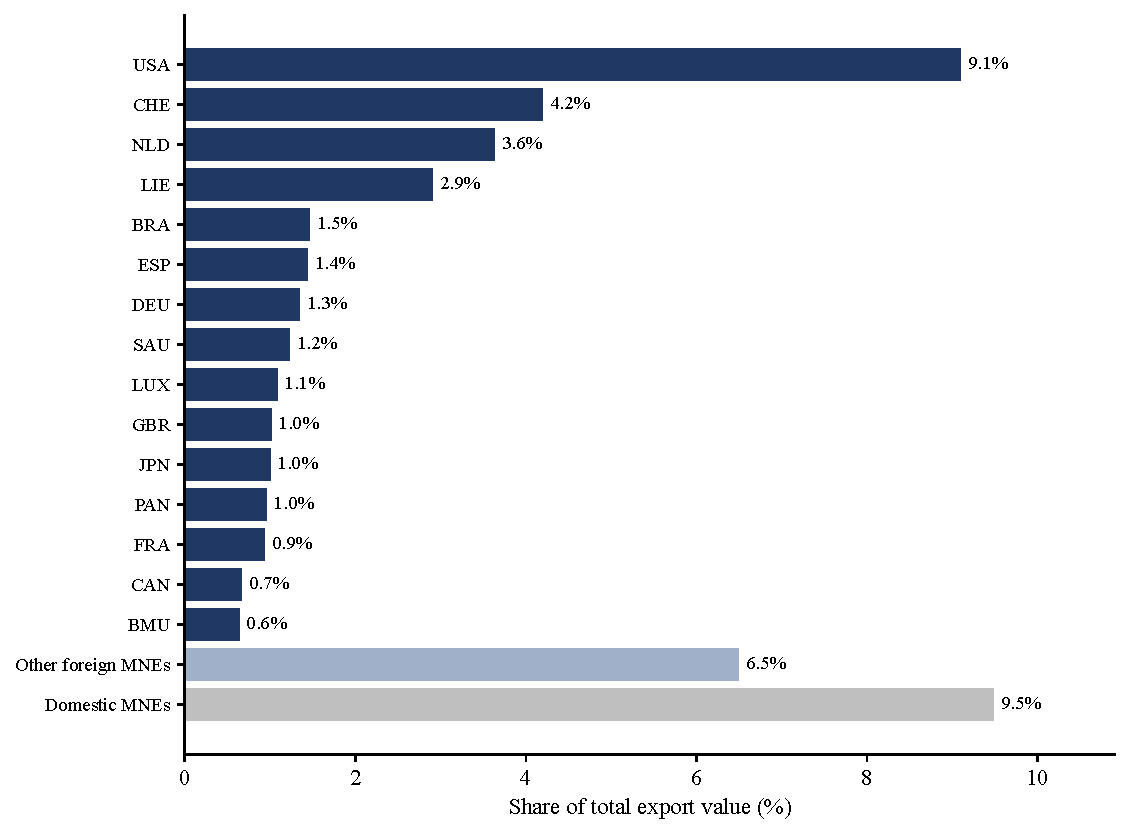
\includegraphics[width=0.85\textwidth,height=0.8\textheight,keepaspectratio]{figures/agro/fig_wp1a_parent_share_total.pdf}%
  \caption{Agriculture: Share of Total Exports, by Parent Country}%
  \label{fig:f4t_agro}%
  \par\vspace{2pt}%
  \parbox{0.92\textwidth}{\footnotesize %
  \textit{Notes:} Percent of total agricultural export value shipped by foreign MNEs of each parent country, other foreign MNEs and domestic MNEs; the remainder is local firms.\\[3pt]%
  \textit{Source:} Authors' calculations based on customs data matched to Orbis and Dun \& Bradstreet.}%
  \end{figure}
% ---- Table: Agriculture: Share of Total Exports, by Parent Country
\begin{table}[H]\centering\small%
  \caption{Agriculture: Share of Total Exports, by Parent Country}%
  \label{tab:f4tn_agro}%
  \adjustbox{max width=\textwidth, max totalheight=0.8\textheight}{\begin{tabular}{lr}
\toprule
Exporter type / parent country & Share of total exports (\%) \\
\midrule
USA & 9.1 \\
CHE & 4.2 \\
NLD & 3.6 \\
LIE & 2.9 \\
BRA & 1.5 \\
ESP & 1.4 \\
DEU & 1.3 \\
SAU & 1.2 \\
LUX & 1.1 \\
GBR & 1.0 \\
JPN & 1.0 \\
PAN & 1.0 \\
FRA & 0.9 \\
CAN & 0.7 \\
BMU & 0.6 \\
Other foreign MNEs & 6.5 \\
Domestic MNEs & 9.5 \\
\midrule
All MNEs & 47.6 \\
Local firms & 52.4 \\
\bottomrule
\end{tabular}
}%
  \par\vspace{3pt}%
  \begin{minipage}{0.95\textwidth}\footnotesize %
  \textit{Notes:} Percent of total agricultural export value, by type of exporter and parent country.\\[3pt]%
  \textit{Source:} Authors' calculations based on customs data matched to Orbis and Dun \& Bradstreet.%
  \end{minipage}%
  \end{table}

\subsection{Parent Region and Destination Region}
% ---- Table: Agriculture: Multinational Exports by Parent Region and Destination Region: Export Value
\begin{table}[H]\centering\small%
  \caption{Agriculture: Multinational Exports by Parent Region and Destination Region: Export Value}%
  \label{tab:reg_value_agro}%
  \adjustbox{max width=\textwidth, max totalheight=0.8\textheight}{\begin{tabular}{lrrrrrrrr}
\toprule
Parent region / Destination region & Latin America & North America & Europe & Asia & Africa & Oceania & Rest of World & Total \\
\midrule
Latin America & 1.0 & 0.6 & 0.7 & 1.0 & 0.1 & 0.0 & 0.0 & 3.4 \\
North America & 3.4 & 0.5 & 0.7 & 1.8 & 0.6 & 0.0 & 0.0 & 7.1 \\
Europe & 3.8 & 1.2 & 3.0 & 4.5 & 1.2 & 0.1 & 0.0 & 13.8 \\
Asia & 0.4 & 0.8 & 0.7 & 0.8 & 0.1 & 0.0 & 0.0 & 2.8 \\
Africa & 0.0 & 0.0 & 0.0 & 0.0 & 0.0 & 0.0 & 0.0 & 0.1 \\
Oceania & 0.0 & 0.0 & 0.0 & 0.0 & 0.0 & 0.0 & 0.0 & 0.0 \\
Rest of World & 0.0 & 0.0 & 0.0 & 0.0 & 0.0 & 0.0 & 0.0 & 0.0 \\
Domestic MNEs & 1.5 & 1.0 & 1.4 & 2.5 & 0.6 & 0.1 & 0.0 & 7.1 \\
Local firms & 9.5 & 6.7 & 11.0 & 10.8 & 2.5 & 0.5 & 0.1 & 41.1 \\
\midrule
Total & 19.7 & 10.9 & 17.5 & 21.5 & 5.0 & 0.6 & 0.1 & 75.4 \\
\bottomrule
\end{tabular}
}%
  \par\vspace{3pt}%
  \begin{minipage}{0.95\textwidth}\footnotesize %
  \textit{Notes:} Values are annual averages in US\$ billion. Rows: region of the ultimate parent; columns: destination region.\\[3pt]%
  \textit{Source:} Authors' calculations based on customs data matched to Orbis and Dun \& Bradstreet.%
  \end{minipage}%
  \end{table}
% ---- Table: Agriculture: Multinational Exports by Parent Region and Destination Region: Row Percentages
\begin{table}[H]\centering\small%
  \caption{Agriculture: Multinational Exports by Parent Region and Destination Region: Row Percentages}%
  \label{tab:reg_rowpct_agro}%
  \adjustbox{max width=\textwidth, max totalheight=0.8\textheight}{\begin{tabular}{lrrrrrrrr}
\toprule
Parent region / Destination region & Latin America & North America & Europe & Asia & Africa & Oceania & Rest of World & Total \\
\midrule
Latin America & 30.0 & 17.1 & 20.5 & 29.3 & 2.8 & 0.3 & 0.1 & 100.0 \\
North America & 47.9 & 8.3 & 10.2 & 25.6 & 7.6 & 0.1 & 0.4 & 100.0 \\
Europe & 27.3 & 10.1 & 22.0 & 31.6 & 8.2 & 0.6 & 0.2 & 100.0 \\
Asia & 14.2 & 29.2 & 24.7 & 29.1 & 2.4 & 0.3 & 0.2 & 100.0 \\
Africa & 29.5 & 15.3 & 30.8 & 13.1 & 9.2 & 0.3 & 1.8 & 100.0 \\
Oceania & 59.2 & 21.5 & 8.5 & 6.1 & 0.7 & 4.1 & 0.0 & 100.0 \\
Rest of World & 17.8 & 36.0 & 28.7 & 16.8 & 0.0 & 0.7 & 0.0 & 100.0 \\
Domestic MNEs & 20.5 & 16.0 & 20.4 & 34.9 & 7.0 & 1.1 & 0.1 & 100.0 \\
Local firms & 22.8 & 17.9 & 26.8 & 25.6 & 5.6 & 1.1 & 0.2 & 100.0 \\
\bottomrule
\end{tabular}
}%
  \par\vspace{3pt}%
  \begin{minipage}{0.95\textwidth}\footnotesize %
  \textit{Notes:} Percent of each group's exports, by destination region (rows add to 100). Domestic MNEs and local firms are shown for comparison.\\[3pt]%
  \textit{Source:} Authors' calculations based on customs data matched to Orbis and Dun \& Bradstreet.%
  \end{minipage}%
  \end{table}
% ---- Table: Agriculture: Multinational Exports by Parent Region and Destination Region: Column Percentages
\begin{table}[H]\centering\small%
  \caption{Agriculture: Multinational Exports by Parent Region and Destination Region: Column Percentages}%
  \label{tab:reg_colpct_agro}%
  \adjustbox{max width=\textwidth, max totalheight=0.8\textheight}{\begin{tabular}{lrrrrrrr}
\toprule
Parent region / Destination region & Latin America & North America & Europe & Asia & Africa & Oceania & Rest of World \\
\midrule
Latin America & 5.3 & 4.9 & 3.9 & 4.7 & 2.0 & 1.5 & 3.4 \\
North America & 16.8 & 4.7 & 3.9 & 8.3 & 11.1 & 0.8 & 19.1 \\
Europe & 18.7 & 11.2 & 16.5 & 20.0 & 23.5 & 13.4 & 17.8 \\
Asia & 2.1 & 6.9 & 4.0 & 3.9 & 1.5 & 1.2 & 3.5 \\
Africa & 0.2 & 0.1 & 0.2 & 0.1 & 0.2 & 0.0 & 1.5 \\
Oceania & 0.1 & 0.1 & 0.0 & 0.0 & 0.0 & 0.2 & 0.0 \\
Rest of World & 0.0 & 0.0 & 0.0 & 0.0 & 0.0 & 0.0 & 0.0 \\
Domestic MNEs & 8.0 & 10.0 & 8.6 & 12.5 & 11.4 & 12.8 & 7.2 \\
Local firms & 48.9 & 62.0 & 62.8 & 50.5 & 50.2 & 70.1 & 47.5 \\
\midrule
Total & 100.0 & 100.0 & 100.0 & 100.0 & 100.0 & 100.0 & 100.0 \\
\bottomrule
\end{tabular}
}%
  \par\vspace{3pt}%
  \begin{minipage}{0.95\textwidth}\footnotesize %
  \textit{Notes:} Percent of the exports reaching each destination region, by parent region (columns add to 100).\\[3pt]%
  \textit{Source:} Authors' calculations based on customs data matched to Orbis and Dun \& Bradstreet.%
  \end{minipage}%
  \end{table}
% ---- Figure: Agriculture: Multinational Exports by Parent Region and Destination Region
\begin{figure}[H]\centering%
  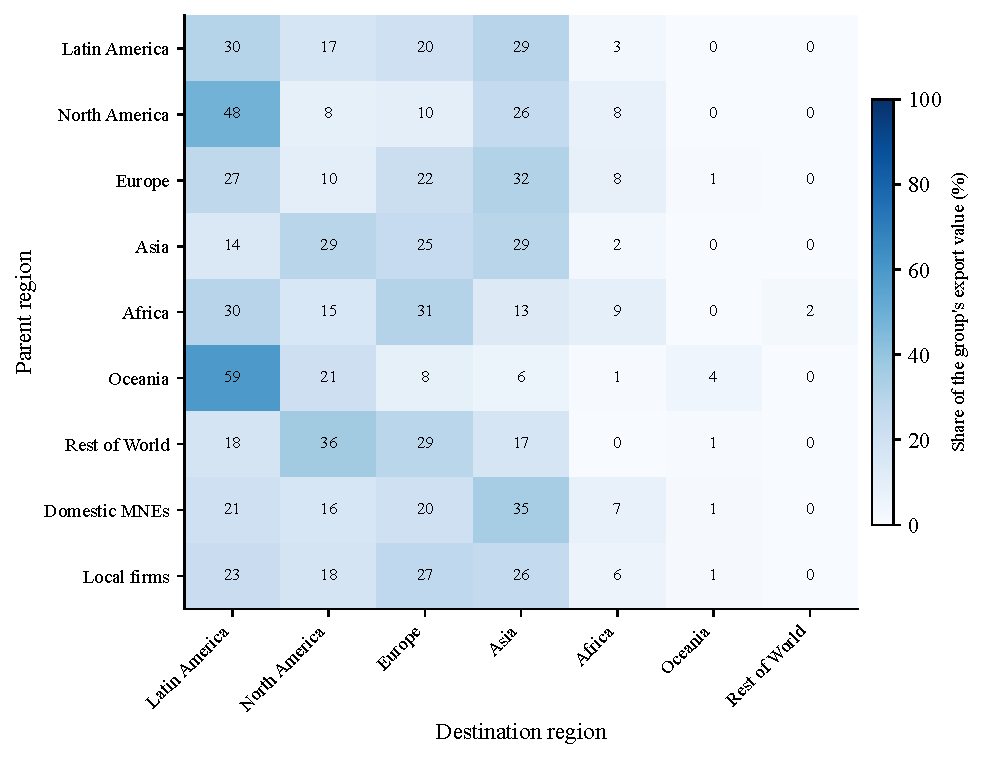
\includegraphics[width=0.9\textwidth,height=0.8\textheight,keepaspectratio]{figures/agro/fig_wp1d_heatmap_region_rowpct.pdf}%
  \caption{Agriculture: Multinational Exports by Parent Region and Destination Region}%
  \label{fig:reg_hm_agro}%
  \par\vspace{2pt}%
  \parbox{0.92\textwidth}{\footnotesize %
  \textit{Notes:} Percent of each group's exports, by destination region (rows add to 100).\\[3pt]%
  \textit{Source:} Authors' calculations based on customs data matched to Orbis and Dun \& Bradstreet.}%
  \end{figure}
% ---- Table: Agriculture: Foreign-Multinational Exports by Exporting Country and Destination Region
\begin{table}[H]\centering\small%
  \caption{Agriculture: Foreign-Multinational Exports by Exporting Country and Destination Region}%
  \label{tab:odr_f_agro}%
  \adjustbox{max width=\textwidth, max totalheight=0.8\textheight}{\begin{tabular}{lrrrrrrrr}
\toprule
Origin \ Destination region & Latin America & North America & Europe & Asia & Africa & Oceania & Rest of World & Total \\
\midrule
ARG & 24.3 & 3.2 & 17.2 & 42.4 & 12.6 & 0.3 & 0.0 & 14.4 \\
CHL & 26.6 & 22.8 & 20.3 & 27.8 & 1.1 & 1.3 & 0.0 & 2.2 \\
COL & 18.0 & 41.2 & 27.8 & 9.5 & 0.6 & 1.0 & 2.0 & 2.0 \\
CRI & 31.5 & 36.6 & 29.7 & 1.7 & 0.3 & 0.2 & 0.0 & 1.9 \\
DOM & 25.5 & 58.0 & 13.9 & 2.1 & 0.2 & 0.0 & 0.4 & 0.8 \\
PER & 15.7 & 24.8 & 32.1 & 25.9 & 0.9 & 0.6 & 0.0 & 2.7 \\
PRY & 79.7 & 0.5 & 11.7 & 6.9 & 1.2 & 0.0 & 0.0 & 4.0 \\
SLV & 58.1 & 12.7 & 26.5 & 1.8 & 0.4 & 0.5 & 0.0 & 0.3 \\
URY & 26.0 & 8.8 & 21.2 & 37.5 & 3.9 & 0.1 & 2.4 & 2.3 \\
\bottomrule
\end{tabular}
}%
  \par\vspace{3pt}%
  \begin{minipage}{0.95\textwidth}\footnotesize %
  \textit{Notes:} Percent of each country's foreign-MNE agricultural exports, by destination region (rows add to 100). Last column: foreign-MNE exports. Values are annual averages in US\$ billion.\\[3pt]%
  \textit{Source:} Authors' calculations based on customs data matched to Orbis and Dun \& Bradstreet.%
  \end{minipage}%
  \end{table}
% ---- Table: Agriculture: Local-Firm Exports by Exporting Country and Destination Region
\begin{table}[H]\centering\small%
  \caption{Agriculture: Local-Firm Exports by Exporting Country and Destination Region}%
  \label{tab:odr_l_agro}%
  \adjustbox{max width=\textwidth, max totalheight=0.8\textheight}{\begin{tabular}{lrrrrrrrr}
\toprule
Origin \ Destination region & Latin America & North America & Europe & Asia & Africa & Oceania & Rest of World & Total \\
\midrule
ARG & 21.6 & 5.0 & 23.8 & 36.9 & 11.0 & 1.7 & 0.0 & 20.0 \\
CHL & 17.9 & 27.4 & 24.9 & 28.3 & 1.1 & 0.4 & 0.0 & 3.9 \\
COL & 16.1 & 42.5 & 31.7 & 7.3 & 1.2 & 0.7 & 0.5 & 4.1 \\
CRI & 27.3 & 33.2 & 35.3 & 3.3 & 0.3 & 0.6 & 0.0 & 2.3 \\
DOM & 25.6 & 38.8 & 33.3 & 1.7 & 0.1 & 0.0 & 0.5 & 1.1 \\
PER & 13.7 & 25.8 & 35.5 & 23.4 & 0.5 & 1.0 & 0.0 & 5.0 \\
PRY & 62.9 & 3.1 & 21.7 & 10.8 & 1.4 & 0.0 & 0.0 & 2.1 \\
SLV & 41.9 & 34.7 & 13.4 & 8.8 & 0.2 & 0.8 & 0.2 & 0.8 \\
URY & 33.8 & 4.9 & 23.8 & 27.8 & 7.9 & 0.1 & 1.8 & 1.7 \\
\bottomrule
\end{tabular}
}%
  \par\vspace{3pt}%
  \begin{minipage}{0.95\textwidth}\footnotesize %
  \textit{Notes:} Percent of each country's agricultural exports by local firms, by destination region (rows add to 100). Last column: local-firm exports. Values are annual averages in US\$ billion.\\[3pt]%
  \textit{Source:} Authors' calculations based on customs data matched to Orbis and Dun \& Bradstreet.%
  \end{minipage}%
  \end{table}

\subsection{Parent Country and Destination Country}
% ---- Table: Agriculture: Foreign-Multinational Exports by Parent Country and Destination: Export Value
\begin{table}[H]\centering\small%
  \caption{Agriculture: Foreign-Multinational Exports by Parent Country and Destination: Export Value}%
  \label{tab:cty_value_agro}%
  \adjustbox{max width=\textwidth, max totalheight=0.8\textheight}{\begin{tabular}{lrrrrrrrrrrrr}
\toprule
Parent / Destination & USA & CHN & BRA & ARG & ESP & CHL & JPN & NLD & URY & ITA & Other destinations & Total \\
\midrule
USA & 0.4 & 1.1 & 0.2 & 1.2 & 0.1 & 0.3 & 0.1 & 0.1 & 0.4 & 0.0 & 2.7 & 6.7 \\
CHE & 0.0 & 0.2 & 0.2 & 0.0 & 0.1 & 0.1 & 0.0 & 0.0 & 0.0 & 0.1 & 2.3 & 3.1 \\
NLD & 0.1 & 0.4 & 0.1 & 0.1 & 0.0 & 0.1 & 0.0 & 0.1 & 0.1 & 0.2 & 1.6 & 2.7 \\
LIE & 0.0 & 0.3 & 0.1 & 0.0 & 0.1 & 0.1 & 0.0 & 0.0 & 0.0 & 0.0 & 1.5 & 2.2 \\
BRA & 0.1 & 0.3 & 0.1 & 0.0 & 0.0 & 0.0 & 0.0 & 0.0 & 0.0 & 0.0 & 0.4 & 1.1 \\
ESP & 0.1 & 0.1 & 0.0 & 0.0 & 0.3 & 0.0 & 0.0 & 0.1 & 0.0 & 0.0 & 0.3 & 1.0 \\
DEU & 0.3 & 0.0 & 0.0 & 0.0 & 0.0 & 0.0 & 0.0 & 0.0 & 0.0 & 0.0 & 0.4 & 0.8 \\
SAU & 0.1 & 0.1 & 0.1 & 0.0 & 0.0 & 0.1 & 0.0 & 0.0 & 0.0 & 0.0 & 0.5 & 0.9 \\
LUX & 0.0 & 0.0 & 0.3 & 0.0 & 0.1 & 0.0 & 0.0 & 0.0 & 0.0 & 0.0 & 0.2 & 0.8 \\
GBR & 0.1 & 0.1 & 0.1 & 0.0 & 0.0 & 0.0 & 0.0 & 0.0 & 0.0 & 0.0 & 0.3 & 0.7 \\
Other parents & 1.7 & 0.6 & 0.6 & 0.6 & 0.3 & 0.1 & 0.3 & 0.3 & 0.1 & 0.1 & 2.5 & 7.2 \\
\midrule
Total & 3.0 & 3.2 & 1.9 & 1.9 & 1.0 & 0.9 & 0.6 & 0.7 & 0.7 & 0.6 & 12.7 & 27.2 \\
\bottomrule
\end{tabular}
}%
  \par\vspace{3pt}%
  \begin{minipage}{0.95\textwidth}\footnotesize %
  \textit{Notes:} Values are annual averages in US\$ billion. Ten largest parent countries and ten largest destinations by foreign-MNE export value.\\[3pt]%
  \textit{Source:} Authors' calculations based on customs data matched to Orbis and Dun \& Bradstreet.%
  \end{minipage}%
  \end{table}
% ---- Table: Agriculture: Foreign-Multinational Exports by Parent Country and Destination: Row Percentages
\begin{table}[H]\centering\small%
  \caption{Agriculture: Foreign-Multinational Exports by Parent Country and Destination: Row Percentages}%
  \label{tab:cty_rowpct_agro}%
  \adjustbox{max width=\textwidth, max totalheight=0.8\textheight}{\begin{tabular}{lrrrrrrrrrrrr}
\toprule
Parent / Destination & USA & CHN & BRA & ARG & ESP & CHL & JPN & NLD & URY & ITA & Other destinations & Total \\
\midrule
USA & 7.3 & 15.5 & 3.7 & 16.7 & 1.2 & 4.1 & 1.8 & 1.7 & 5.5 & 0.7 & 41.8 & 100.0 \\
CHE & 1.7 & 6.7 & 7.2 & 0.2 & 2.6 & 3.4 & 0.4 & 1.2 & 0.7 & 3.7 & 72.3 & 100.0 \\
NLD & 3.3 & 14.4 & 5.1 & 3.9 & 1.4 & 3.6 & 0.6 & 2.8 & 2.4 & 5.6 & 57.0 & 100.0 \\
LIE & 1.3 & 14.4 & 6.1 & 0.0 & 2.9 & 2.6 & 0.4 & 0.9 & 0.2 & 2.2 & 69.1 & 100.0 \\
BRA & 11.4 & 31.2 & 4.9 & 1.9 & 1.2 & 1.7 & 1.1 & 4.3 & 0.9 & 2.2 & 39.2 & 100.0 \\
ESP & 15.5 & 8.3 & 3.0 & 0.4 & 26.1 & 2.5 & 3.9 & 5.8 & 0.2 & 2.9 & 31.4 & 100.0 \\
DEU & 37.3 & 0.6 & 1.8 & 0.4 & 3.5 & 0.9 & 5.0 & 4.3 & 0.7 & 1.8 & 43.6 & 100.0 \\
SAU & 6.4 & 12.3 & 6.9 & 0.1 & 2.3 & 15.8 & 0.1 & 2.6 & 0.3 & 2.1 & 51.1 & 100.0 \\
LUX & 6.5 & 2.5 & 40.8 & 0.0 & 8.1 & 2.0 & 2.1 & 0.3 & 2.8 & 4.5 & 30.4 & 100.0 \\
GBR & 8.9 & 16.9 & 8.5 & 0.6 & 3.5 & 2.7 & 2.2 & 2.9 & 2.1 & 0.8 & 50.9 & 100.0 \\
Other parents & 23.1 & 7.9 & 7.9 & 7.5 & 4.0 & 1.5 & 5.5 & 3.5 & 1.8 & 2.0 & 35.4 & 100.0 \\
\bottomrule
\end{tabular}
}%
  \par\vspace{3pt}%
  \begin{minipage}{0.95\textwidth}\footnotesize %
  \textit{Notes:} Percent of each parent country's exports, by destination (rows add to 100). Ten largest parent countries and destinations.\\[3pt]%
  \textit{Source:} Authors' calculations based on customs data matched to Orbis and Dun \& Bradstreet.%
  \end{minipage}%
  \end{table}
% ---- Table: Agriculture: Foreign-Multinational Exports by Parent Country and Destination: Column Percentages
\begin{table}[H]\centering\small%
  \caption{Agriculture: Foreign-Multinational Exports by Parent Country and Destination: Column Percentages}%
  \label{tab:cty_colpct_agro}%
  \adjustbox{max width=\textwidth, max totalheight=0.8\textheight}{\begin{tabular}{lrrrrrrrrrrr}
\toprule
Parent / Destination & USA & CHN & BRA & ARG & ESP & CHL & JPN & NLD & URY & ITA & Other destinations \\
\midrule
USA & 14.7 & 32.0 & 12.9 & 60.5 & 8.2 & 31.2 & 16.7 & 15.5 & 55.8 & 7.1 & 21.4 \\
CHE & 1.6 & 6.3 & 11.6 & 0.3 & 7.8 & 12.0 & 1.7 & 5.3 & 3.3 & 17.6 & 17.1 \\
NLD & 2.7 & 11.9 & 7.1 & 5.6 & 3.6 & 10.8 & 2.3 & 10.6 & 9.7 & 23.1 & 11.6 \\
LIE & 0.8 & 9.5 & 6.8 & 0.0 & 6.1 & 6.2 & 1.1 & 2.7 & 0.6 & 7.3 & 11.3 \\
BRA & 3.7 & 10.4 & 2.8 & 1.1 & 1.3 & 2.1 & 1.6 & 6.5 & 1.5 & 3.7 & 3.2 \\
ESP & 5.0 & 2.7 & 1.7 & 0.2 & 27.4 & 3.0 & 5.6 & 8.6 & 0.3 & 4.8 & 2.5 \\
DEU & 11.2 & 0.2 & 0.9 & 0.2 & 3.5 & 1.0 & 6.8 & 6.0 & 1.0 & 2.7 & 3.3 \\
SAU & 1.7 & 3.4 & 3.3 & 0.0 & 2.1 & 16.1 & 0.2 & 3.3 & 0.4 & 2.9 & 3.5 \\
LUX & 1.6 & 0.6 & 17.0 & 0.0 & 6.4 & 1.8 & 2.3 & 0.3 & 3.4 & 5.5 & 1.8 \\
GBR & 2.0 & 3.9 & 3.3 & 0.2 & 2.6 & 2.2 & 2.3 & 3.1 & 2.3 & 1.0 & 2.9 \\
Other parents & 55.1 & 19.1 & 32.6 & 31.7 & 31.0 & 13.5 & 59.4 & 38.1 & 21.6 & 24.4 & 21.3 \\
\midrule
Total & 100.0 & 100.0 & 100.0 & 100.0 & 100.0 & 100.0 & 100.0 & 100.0 & 100.0 & 100.0 & 100.0 \\
\bottomrule
\end{tabular}
}%
  \par\vspace{3pt}%
  \begin{minipage}{0.95\textwidth}\footnotesize %
  \textit{Notes:} Percent of the foreign-MNE exports reaching each destination, by parent country (columns add to 100). Ten largest parent countries and destinations.\\[3pt]%
  \textit{Source:} Authors' calculations based on customs data matched to Orbis and Dun \& Bradstreet.%
  \end{minipage}%
  \end{table}
% ---- Figure: Agriculture: Destination of Foreign-Multinational Exports: Fifteen Largest Parent Countries and Destinations
\begin{figure}[H]\centering%
  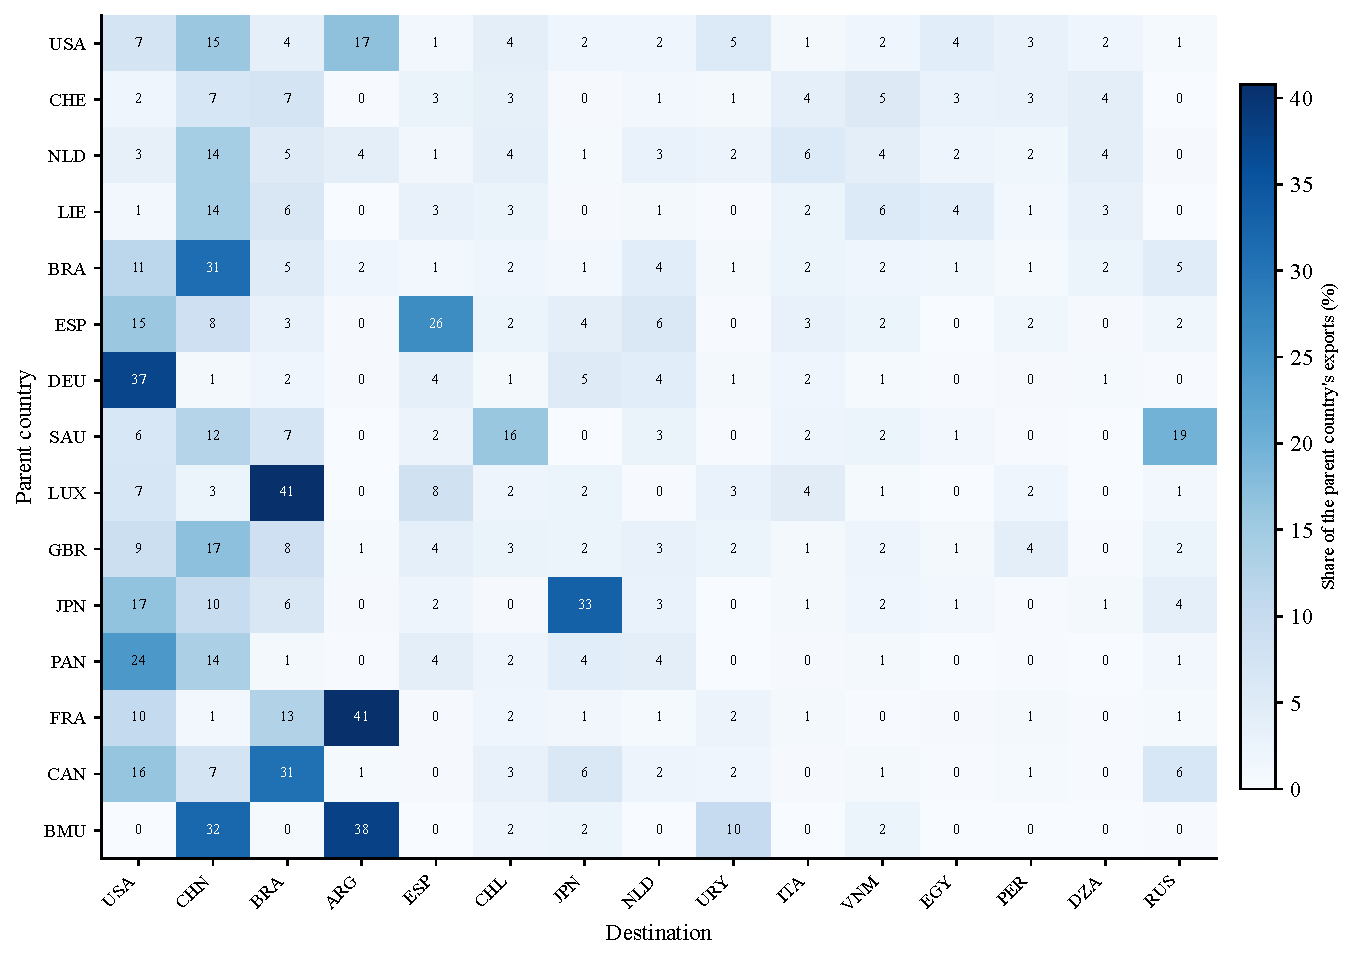
\includegraphics[width=1.0\textwidth,height=0.8\textheight,keepaspectratio]{figures/agro/fig_wp1d_heatmap_country_rowpct.pdf}%
  \caption{Agriculture: Destination of Foreign-Multinational Exports: Fifteen Largest Parent Countries and Destinations}%
  \label{fig:hm_row_agro}%
  \par\vspace{2pt}%
  \parbox{0.92\textwidth}{\footnotesize %
  \textit{Notes:} Percent of each parent country's exports going to each destination (rows add to 100 including other destinations).\\[3pt]%
  \textit{Source:} Authors' calculations based on customs data matched to Orbis and Dun \& Bradstreet.}%
  \end{figure}
% ---- Figure: Agriculture: Foreign-Multinational Exports by Parent Country and Destination: Share of the Total
\begin{figure}[H]\centering%
  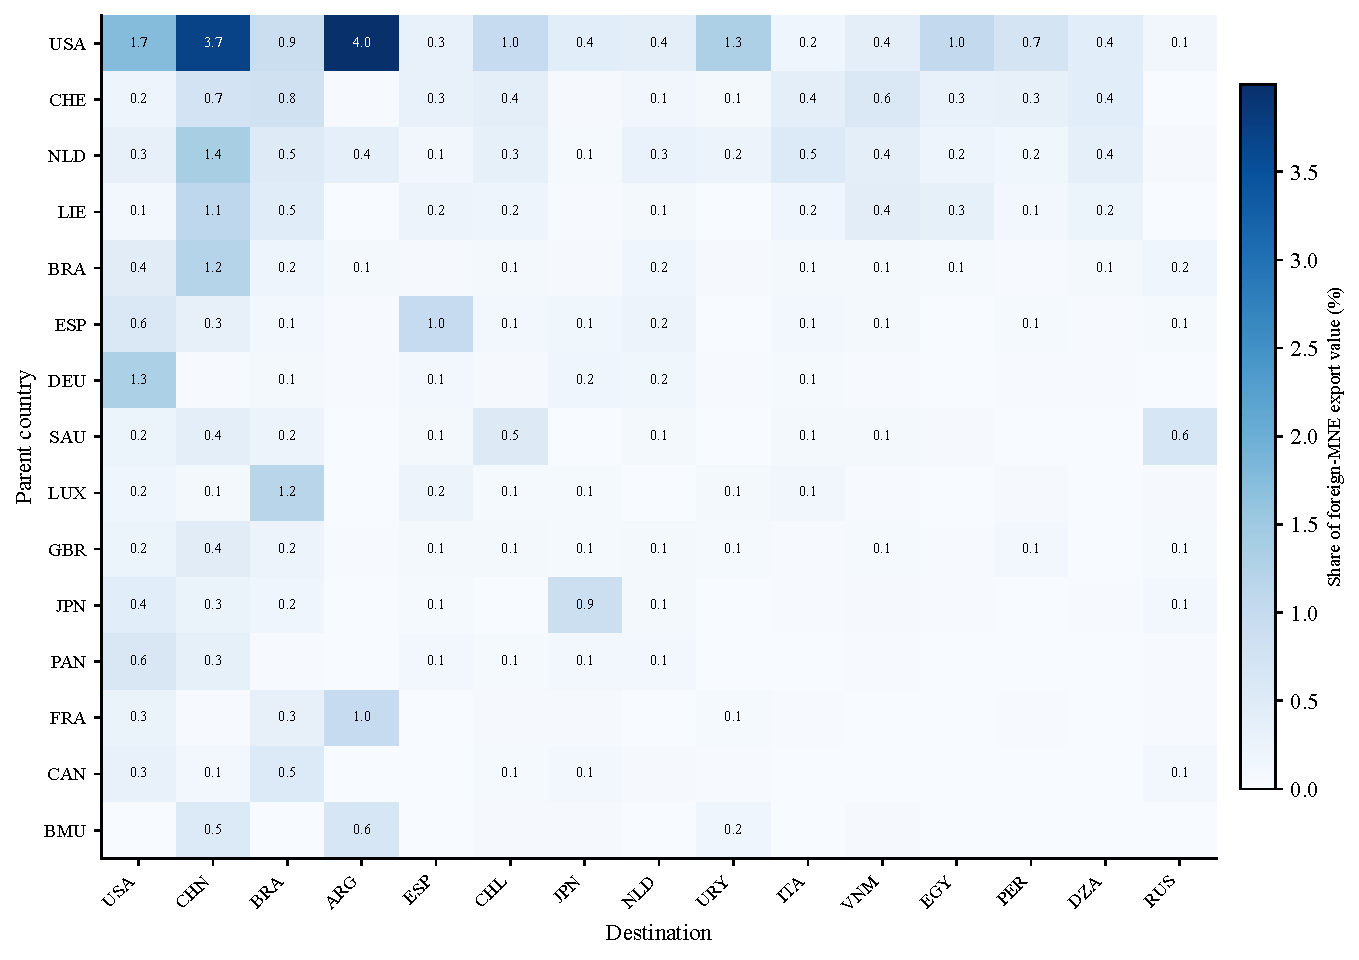
\includegraphics[width=1.0\textwidth,height=0.8\textheight,keepaspectratio]{figures/agro/fig_wp1d_heatmap_country_cellpct.pdf}%
  \caption{Agriculture: Foreign-Multinational Exports by Parent Country and Destination: Share of the Total}%
  \label{fig:hm_cell_agro}%
  \par\vspace{2pt}%
  \parbox{0.92\textwidth}{\footnotesize %
  \textit{Notes:} Percent of all foreign-MNE export value in each parent country and destination pair; fifteen largest parent countries and destinations.\\[3pt]%
  \textit{Source:} Authors' calculations based on customs data matched to Orbis and Dun \& Bradstreet.}%
  \end{figure}

\subsection{Exports to the Parent Country}
% ---- Figure: Agriculture: Share of Foreign-Multinational Exports Shipped to the Parent Country
\begin{figure}[H]\centering%
  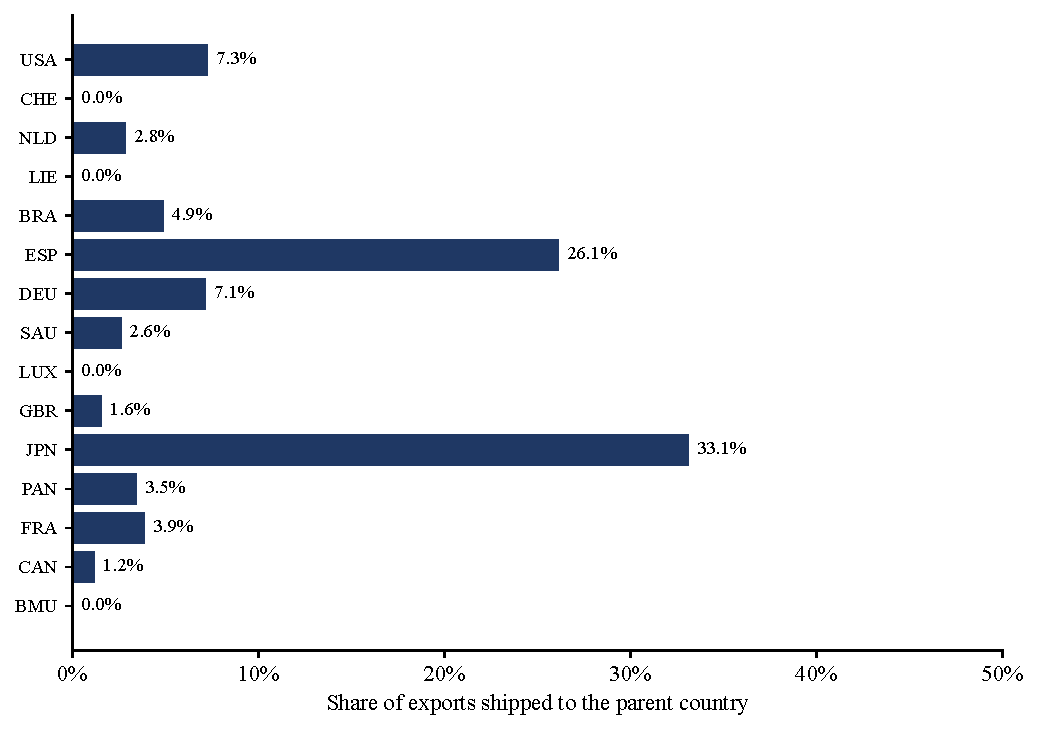
\includegraphics[width=0.85\textwidth,height=0.8\textheight,keepaspectratio]{figures/agro/fig_wp1d_home_share_by_parent.pdf}%
  \caption{Agriculture: Share of Foreign-Multinational Exports Shipped to the Parent Country}%
  \label{fig:home_agro}%
  \par\vspace{2pt}%
  \parbox{0.92\textwidth}{\footnotesize %
  \textit{Notes:} Percent of each parent country's exports shipped to that same country.\\[3pt]%
  \textit{Source:} Authors' calculations based on customs data matched to Orbis and Dun \& Bradstreet.}%
  \end{figure}
% ---- Table: Agriculture: Foreign-Multinational Exports to the Parent Countries, by Parent Country
\begin{table}[H]\centering\small%
  \caption{Agriculture: Foreign-Multinational Exports to the Parent Countries, by Parent Country}%
  \label{tab:pxp_agro}%
  \adjustbox{max width=\textwidth, max totalheight=0.8\textheight}{\begin{tabular}{lrrrrrrrrrrr}
\toprule
Parent / Destination & USA & CHE & NLD & BRA & ESP & DEU & SAU & LUX & GBR & Other destinations & Total \\
\midrule
USA & 7.3 & 0.0 & 1.7 & 3.7 & 1.2 & 0.6 & 1.0 & 0.0 & 0.5 & 84.1 & 100.0 \\
CHE & 1.7 & 0.0 & 1.2 & 7.2 & 2.6 & 0.3 & 3.8 & 0.0 & 0.9 & 82.3 & 100.0 \\
NLD & 3.3 & 0.0 & 2.8 & 5.1 & 1.4 & 0.6 & 1.0 & 0.0 & 0.8 & 85.0 & 100.0 \\
LIE & 1.3 & 0.0 & 0.9 & 6.1 & 2.9 & 0.1 & 3.0 & 0.0 & 0.5 & 85.3 & 100.0 \\
BRA & 11.4 & 0.6 & 4.3 & 4.9 & 1.2 & 5.1 & 0.9 & 0.0 & 1.3 & 70.3 & 100.0 \\
ESP & 15.5 & 0.0 & 5.8 & 3.0 & 26.1 & 1.6 & 0.3 & 0.0 & 1.9 & 45.7 & 100.0 \\
DEU & 37.3 & 0.1 & 4.3 & 1.8 & 3.5 & 7.1 & 0.2 & 0.0 & 1.2 & 44.4 & 100.0 \\
SAU & 6.4 & 0.7 & 2.6 & 6.9 & 2.3 & 1.2 & 2.6 & 0.0 & 1.5 & 75.7 & 100.0 \\
LUX & 6.5 & 0.1 & 0.3 & 40.8 & 8.1 & 0.7 & 0.0 & 0.0 & 0.4 & 43.1 & 100.0 \\
GBR & 8.9 & 0.2 & 2.9 & 8.5 & 3.5 & 2.1 & 0.0 & 0.0 & 1.6 & 72.3 & 100.0 \\
Other parents & 23.1 & 0.3 & 3.5 & 7.9 & 4.0 & 2.0 & 0.3 & 0.0 & 1.9 & 56.9 & 100.0 \\
\bottomrule
\end{tabular}
}%
  \par\vspace{3pt}%
  \begin{minipage}{0.95\textwidth}\footnotesize %
  \textit{Notes:} Percent of each parent country's exports, by destination (rows add to 100). Destinations are the ten largest parent countries; the diagonal is the share shipped to the parent's own country.\\[3pt]%
  \textit{Source:} Authors' calculations based on customs data matched to Orbis and Dun \& Bradstreet.%
  \end{minipage}%
  \end{table}
% ---- Figure: Agriculture: Share of Foreign-Multinational Exports Shipped to the Parent Jurisdiction, Consolidated Parents
\begin{figure}[H]\centering%
  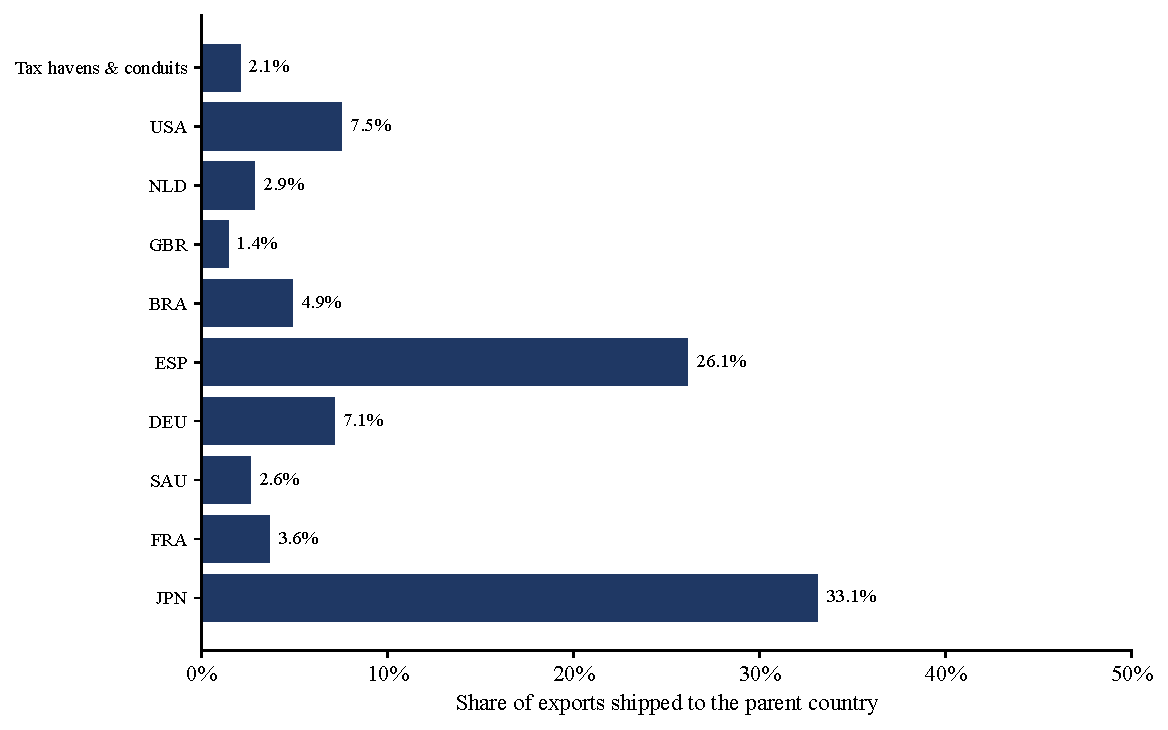
\includegraphics[width=0.85\textwidth,height=0.8\textheight,keepaspectratio]{figures/agro/fig_wp1d_home_share_by_parent_consolidated.pdf}%
  \caption{Agriculture: Share of Foreign-Multinational Exports Shipped to the Parent Jurisdiction, Consolidated Parents}%
  \label{fig:homec_agro}%
  \par\vspace{2pt}%
  \parbox{0.92\textwidth}{\footnotesize %
  \textit{Notes:} Percent of each parent's exports shipped to its own jurisdiction. Dependencies are assigned to their sovereign state and tax havens and conduit jurisdictions are pooled.\\[3pt]%
  \textit{Source:} Authors' calculations based on customs data matched to Orbis and Dun \& Bradstreet.}%
  \end{figure}
% ---- Table: Agriculture: Share of Foreign-Multinational Exports Shipped to the Parent Jurisdiction, Consolidated Parents
\begin{table}[H]\centering\small%
  \caption{Agriculture: Share of Foreign-Multinational Exports Shipped to the Parent Jurisdiction, Consolidated Parents}%
  \label{tab:homec_t_agro}%
  \adjustbox{max width=\textwidth, max totalheight=0.8\textheight}{\begin{tabular}{lrr}
\toprule
Consolidated parent & Home share (\%) & Exports (US\$bn/yr) \\
\midrule
Tax havens \& conduits & 2.1 & 7.1 \\
USA & 7.5 & 6.7 \\
NLD & 2.9 & 2.8 \\
GBR & 1.4 & 1.3 \\
BRA & 4.9 & 1.1 \\
ESP & 26.1 & 1.0 \\
DEU & 7.1 & 0.8 \\
SAU & 2.6 & 0.9 \\
FRA & 3.6 & 0.7 \\
JPN & 33.1 & 0.6 \\
\bottomrule
\end{tabular}
}%
  \par\vspace{3pt}%
  \begin{minipage}{0.95\textwidth}\footnotesize %
  \textit{Notes:} Home share: percent of the parent's exports shipped to its own jurisdiction. Values are annual averages in US\$ billion.\\[3pt]%
  \textit{Source:} Authors' calculations based on customs data matched to Orbis and Dun \& Bradstreet.%
  \end{minipage}%
  \end{table}
% ---- Figure: Agriculture: Share of Foreign-Multinational Exports Shipped to the Parent Jurisdiction
\begin{figure}[H]\centering%
  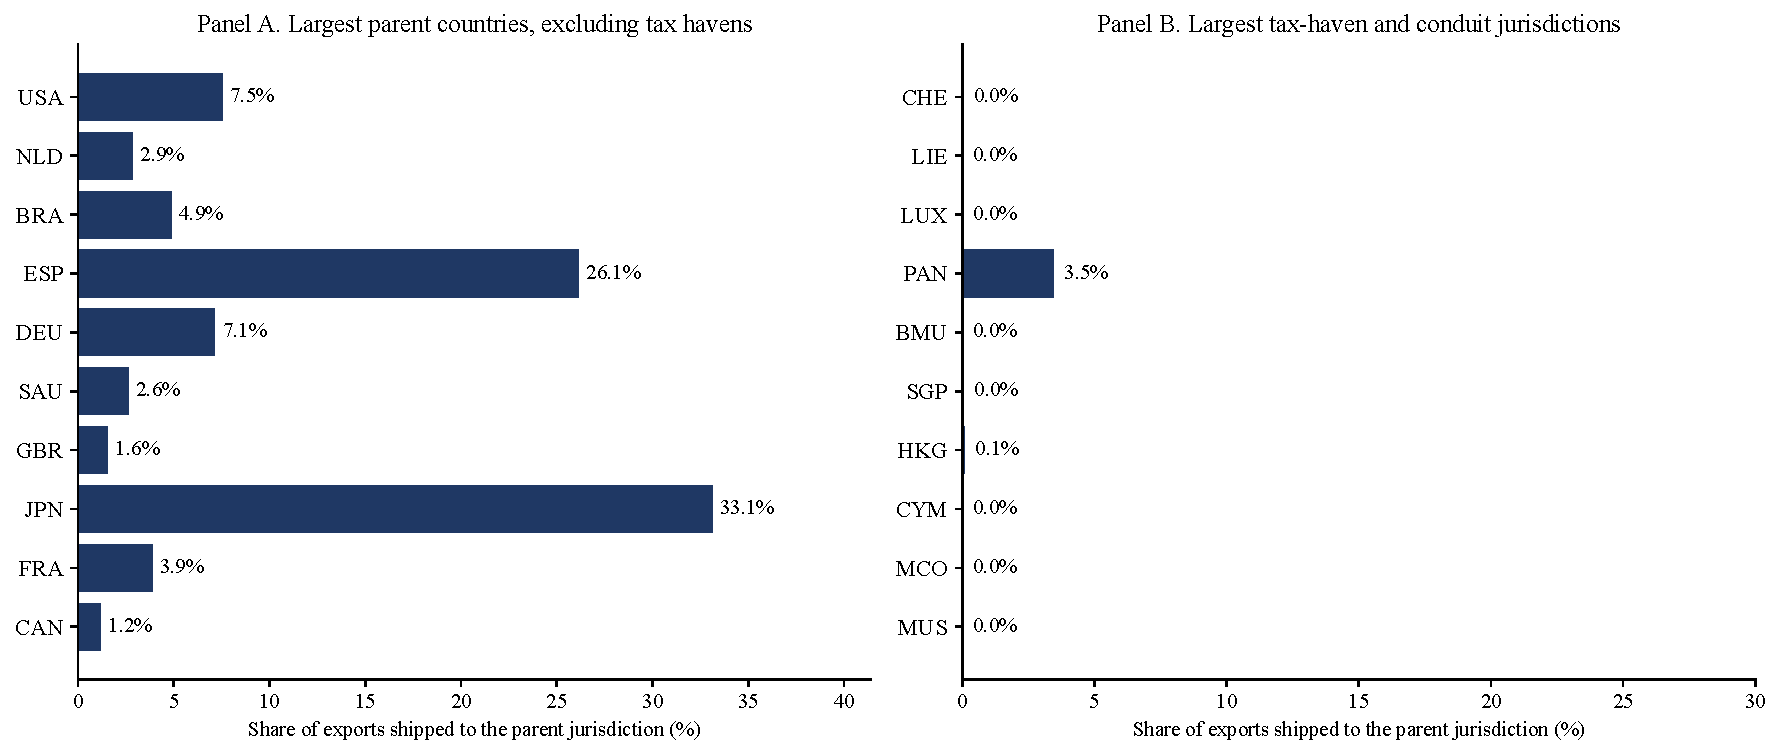
\includegraphics[width=1.0\textwidth,height=0.8\textheight,keepaspectratio]{figures/agro/fig_wp1d_home_share_haven_panels.pdf}%
  \caption{Agriculture: Share of Foreign-Multinational Exports Shipped to the Parent Jurisdiction}%
  \label{fig:homeh_agro}%
  \par\vspace{2pt}%
  \parbox{0.92\textwidth}{\footnotesize %
  \textit{Notes:} Percent of each parent jurisdiction's exports shipped to that same jurisdiction. Panel A: largest parent countries, excluding tax havens; dependencies are assigned to their sovereign state. Panel B: largest tax-haven and conduit jurisdictions.\\[3pt]%
  \textit{Source:} Authors' calculations based on customs data matched to Orbis and Dun \& Bradstreet.}%
  \end{figure}
% ---- Table: Agriculture: Share of Foreign-Multinational Exports Shipped to the Parent Jurisdiction
\begin{table}[H]\centering\small%
  \caption{Agriculture: Share of Foreign-Multinational Exports Shipped to the Parent Jurisdiction}%
  \label{tab:homeh_t_agro}%
  \adjustbox{max width=\textwidth, max totalheight=0.8\textheight}{\begin{tabular}{llrr}
\toprule
Panel & Parent & Home share (\%) & Exports (US\$bn/yr) \\
\midrule
Panel A & USA & 7.5 & 6.7 \\
Panel A & NLD & 2.9 & 2.7 \\
Panel A & BRA & 4.9 & 1.1 \\
Panel A & ESP & 26.1 & 1.0 \\
Panel A & DEU & 7.1 & 0.8 \\
Panel A & SAU & 2.6 & 0.9 \\
Panel A & GBR & 1.6 & 0.7 \\
Panel A & JPN & 33.1 & 0.6 \\
Panel A & FRA & 3.9 & 0.7 \\
Panel A & CAN & 1.2 & 0.4 \\
\midrule
Panel B & CHE & 0.0 & 3.1 \\
Panel B & LIE & 0.0 & 2.2 \\
Panel B & LUX & 0.0 & 0.8 \\
Panel B & PAN & 3.5 & 0.6 \\
Panel B & BMU & 0.0 & 0.5 \\
Panel B & SGP & 0.0 & 0.2 \\
Panel B & HKG & 0.1 & 0.2 \\
Panel B & CYM & 0.0 & 0.1 \\
Panel B & MCO & 0.0 & 0.1 \\
Panel B & MUS & 0.0 & 0.0 \\
\bottomrule
\end{tabular}
}%
  \par\vspace{3pt}%
  \begin{minipage}{0.95\textwidth}\footnotesize %
  \textit{Notes:} Home share: percent of the parent's exports shipped to its own jurisdiction. Panel A: largest parent countries, excluding tax havens. Panel B: largest tax-haven and conduit jurisdictions. Values are annual averages in US\$ billion.\\[3pt]%
  \textit{Source:} Authors' calculations based on customs data matched to Orbis and Dun \& Bradstreet.%
  \end{minipage}%
  \end{table}

\subsection{Destination Markets}
% ---- Figure: Agriculture: Exports to the United States, by Type of Exporter and Exporting Country
\begin{figure}[H]\centering%
  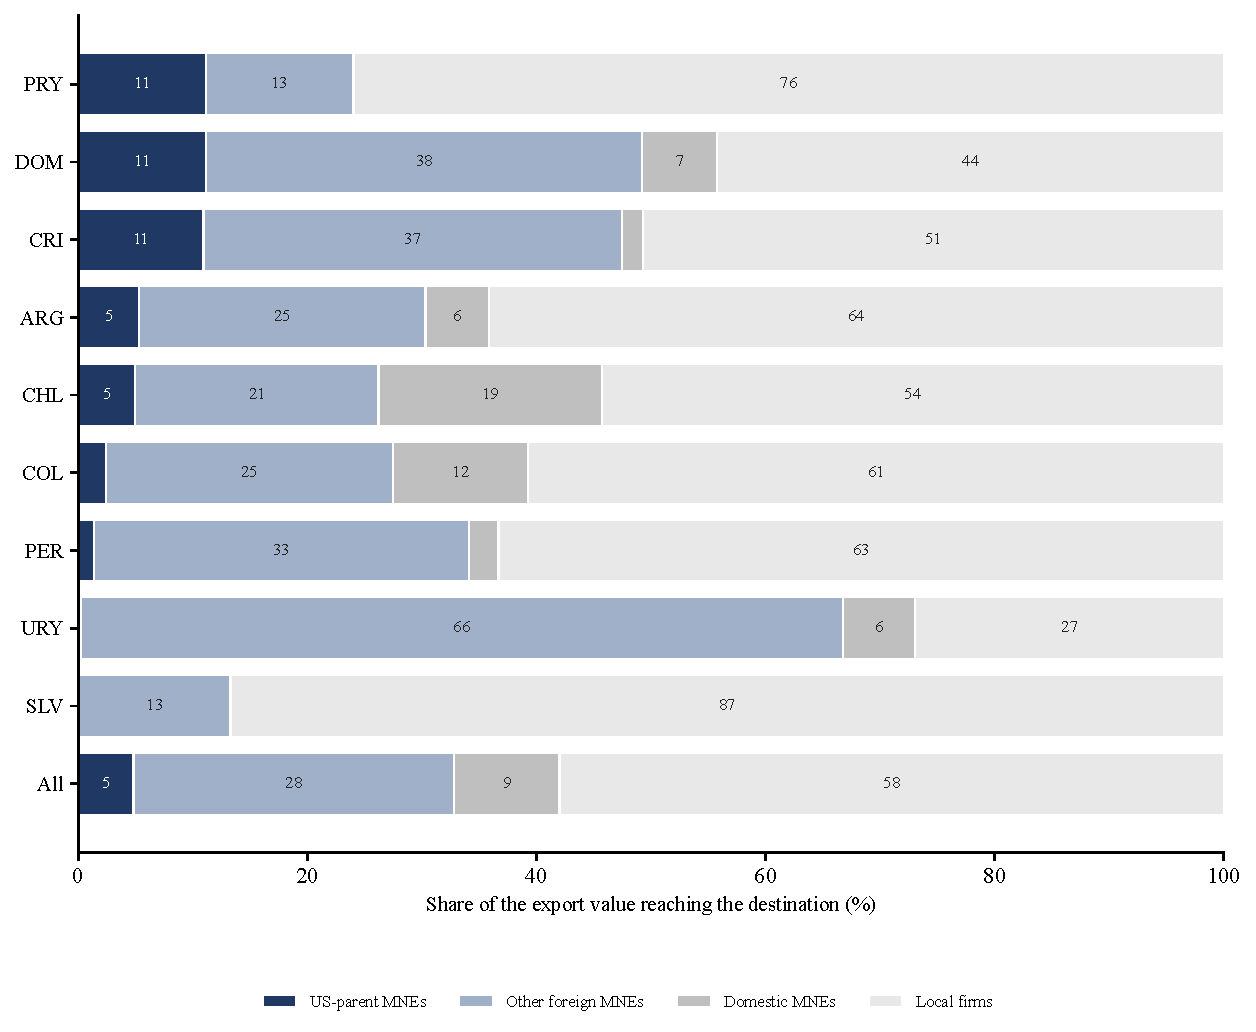
\includegraphics[width=0.9\textwidth,height=0.8\textheight,keepaspectratio]{figures/agro/fig_wp3_to_usa_carriers.pdf}%
  \caption{Agriculture: Exports to the United States, by Type of Exporter and Exporting Country}%
  \label{fig:to_usa_f_agro}%
  \par\vspace{2pt}%
  \parbox{0.92\textwidth}{\footnotesize %
  \textit{Notes:} Percent of each country's agricultural exports to the United States, by type of exporter.\\[3pt]%
  \textit{Source:} Authors' calculations based on customs data matched to Orbis and Dun \& Bradstreet.}%
  \end{figure}
% ---- Table: Agriculture: Exports to the United States, by Type of Exporter and Exporting Country
\begin{table}[H]\centering\small%
  \caption{Agriculture: Exports to the United States, by Type of Exporter and Exporting Country}%
  \label{tab:to_usa_agro}%
  \adjustbox{max width=\textwidth, max totalheight=0.8\textheight}{\begin{tabular}{lrrrrr}
\toprule
Origin & Exports to the USA (US\$bn/yr) & US-parent MNEs (\%) & Other foreign MNEs (\%) & Domestic MNEs (\%) & Local firms (\%) \\
\midrule
PRY & 0.1 & 11.2 & 12.8 & 0.1 & 76.0 \\
DOM & 0.9 & 11.2 & 38.1 & 6.6 & 44.2 \\
CRI & 1.5 & 10.9 & 36.5 & 1.8 & 50.7 \\
ARG & 1.4 & 5.3 & 25.0 & 5.5 & 64.1 \\
CHL & 1.8 & 5.0 & 21.2 & 19.5 & 54.3 \\
COL & 2.7 & 2.4 & 25.1 & 11.8 & 60.7 \\
PER & 1.8 & 1.4 & 32.7 & 2.6 & 63.3 \\
URY & 0.3 & 0.2 & 66.5 & 6.3 & 26.9 \\
SLV & 0.3 & 0.1 & 13.2 & 0.0 & 86.7 \\
\midrule
All & 10.7 & 4.8 & 28.0 & 9.2 & 58.0 \\
\bottomrule
\end{tabular}
}%
  \par\vspace{3pt}%
  \begin{minipage}{0.95\textwidth}\footnotesize %
  \textit{Notes:} Percent of each country's agricultural exports to the United States, by type of exporter. Values are annual averages in US\$ billion.\\[3pt]%
  \textit{Source:} Authors' calculations based on customs data matched to Orbis and Dun \& Bradstreet.%
  \end{minipage}%
  \end{table}
% ---- Figure: Agriculture: Ownership of Exports to the Main Destination Markets
\begin{figure}[H]\centering%
  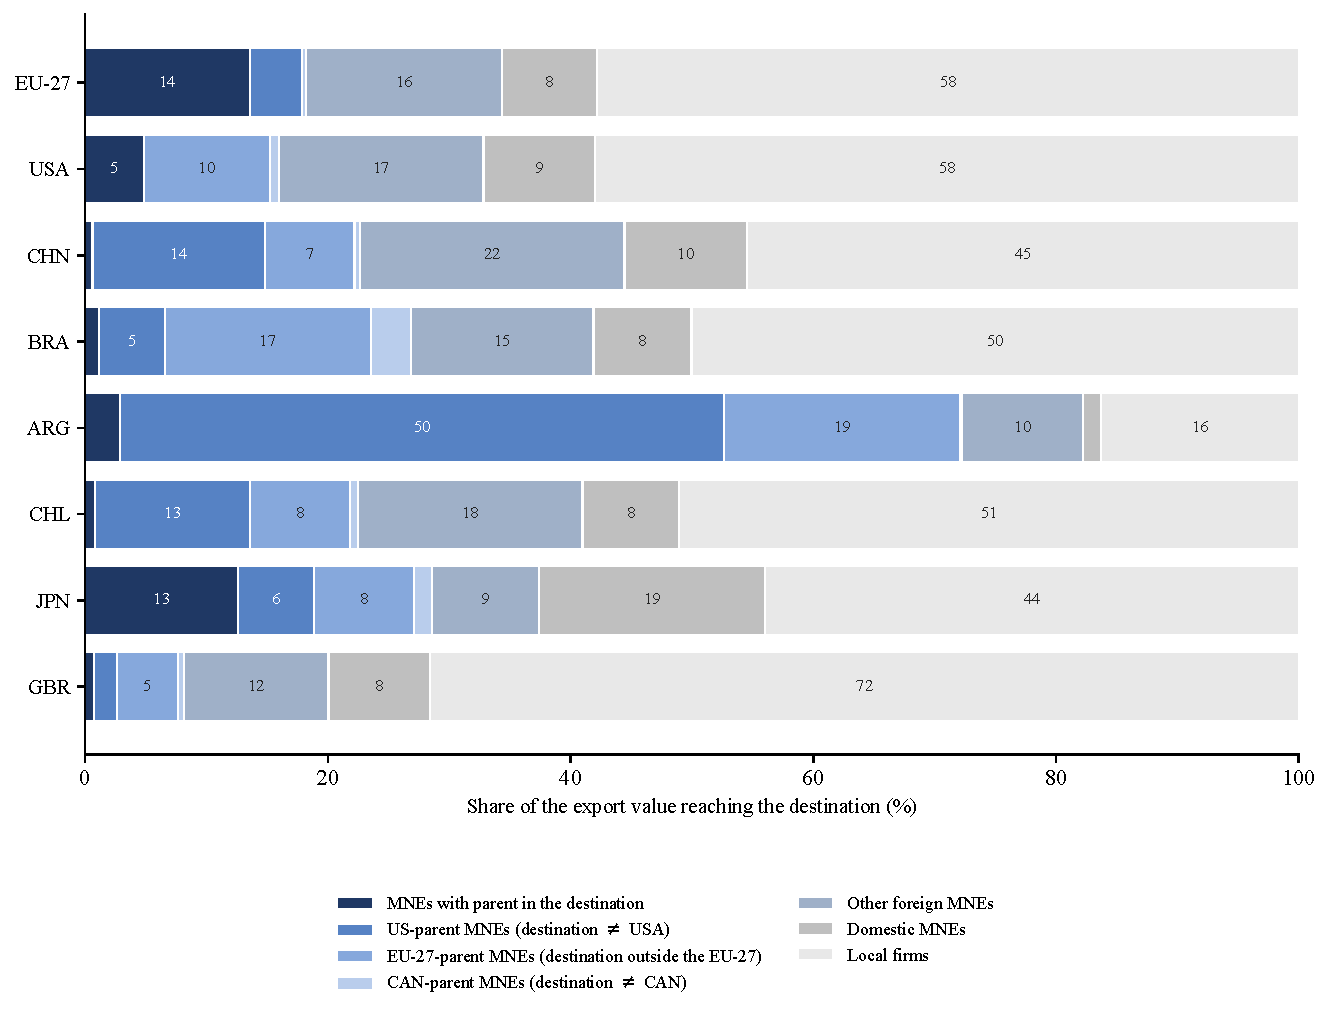
\includegraphics[width=0.95\textwidth,height=0.8\textheight,keepaspectratio]{figures/agro/fig_wp3_dest_carriers.pdf}%
  \caption{Agriculture: Ownership of Exports to the Main Destination Markets}%
  \label{fig:dest_f_agro}%
  \par\vspace{2pt}%
  \parbox{0.92\textwidth}{\footnotesize %
  \textit{Notes:} Percent of the export value reaching each destination, by type of exporter. The first segment is exports by MNEs whose parent is located in that destination. EU-27 member states are pooled.\\[3pt]%
  \textit{Source:} Authors' calculations based on customs data matched to Orbis and Dun \& Bradstreet.}%
  \end{figure}
% ---- Table: Agriculture: Ownership of Exports to the Main Destination Markets
\begin{table}[H]\centering\footnotesize%
  \caption{Agriculture: Ownership of Exports to the Main Destination Markets}%
  \label{tab:dest_agro}%
  \adjustbox{max width=\textwidth, max totalheight=0.8\textheight}{\begin{tabular}{lrrrrrrrr}
\toprule
Destination & \multicolumn{1}{p{1.5cm}}{\raggedright Exports (US\$bn/yr)} & \multicolumn{1}{p{2.2cm}}{\raggedright MNEs with parent in the destination (\%)} & \multicolumn{1}{p{1.6cm}}{\raggedright US-parent MNEs (\%)} & \multicolumn{1}{p{1.6cm}}{\raggedright EU-27-parent MNEs (\%)} & \multicolumn{1}{p{1.6cm}}{\raggedright CAN-parent MNEs (\%)} & \multicolumn{1}{p{1.6cm}}{\raggedright Other foreign MNEs (\%)} & \multicolumn{1}{p{1.6cm}}{\raggedright Domestic MNEs (\%)} & \multicolumn{1}{p{1.5cm}}{\raggedright Local firms (\%)} \\
\midrule
EU-27 & 13.8 & 13.6 & 4.3 & -- & 0.3 & 16.1 & 7.8 & 57.8 \\
USA & 10.7 & 4.8 & -- & 10.4 & 0.8 & 16.8 & 9.2 & 58.0 \\
CHN & 7.5 & 0.6 & 14.2 & 7.4 & 0.5 & 21.8 & 10.1 & 45.4 \\
BRA & 5.1 & 1.2 & 5.4 & 17.0 & 3.3 & 15.1 & 8.1 & 50.0 \\
ARG & 2.5 & 2.9 & 49.8 & 19.5 & 0.1 & 10.0 & 1.5 & 16.3 \\
CHL & 2.4 & 0.8 & 12.8 & 8.2 & 0.7 & 18.5 & 8.0 & 51.1 \\
JPN & 1.9 & 12.6 & 6.2 & 8.2 & 1.5 & 8.9 & 18.6 & 44.0 \\
GBR & 1.9 & 0.7 & 1.9 & 5.0 & 0.5 & 11.9 & 8.4 & 71.6 \\
\bottomrule
\end{tabular}
}%
  \par\vspace{3pt}%
  \begin{minipage}{0.95\textwidth}\footnotesize %
  \textit{Notes:} Percent of the export value reaching each destination, by type of exporter. EU-27 member states are pooled. Values are annual averages in US\$ billion.\\[3pt]%
  \textit{Source:} Authors' calculations based on customs data matched to Orbis and Dun \& Bradstreet.%
  \end{minipage}%
  \end{table}
% ---- Table: Agriculture: Main Products Shipped by US-Parent Multinationals to the United States
\begin{table}[H]\centering\footnotesize%
  \caption{Agriculture: Main Products Shipped by US-Parent Multinationals to the United States}%
  \label{tab:us_home_agro}%
  \adjustbox{max width=\textwidth, max totalheight=0.8\textheight}{\begin{tabular}{llrrrrrl}
\toprule
HS6 & Description & \multicolumn{1}{p{1.7cm}}{\raggedright US-parent exports to the USA (US\$bn/yr)} & \multicolumn{1}{p{1.7cm}}{\raggedright \% of all US-parent exports to the USA} & \multicolumn{1}{p{2.0cm}}{\raggedright \% of US-parent exports of the product going to the USA} & \multicolumn{1}{p{1.9cm}}{\raggedright All exports of the product to the USA (US\$bn/yr)} & \multicolumn{1}{p{2.2cm}}{\raggedright US-parent share of exports of the product to the USA (\%)} & \multicolumn{1}{p{2.6cm}}{\raggedright Main origins of the US-parent shipments (\% of the line)} \\
\midrule
080430 & Pineapples, fresh/dried & 0.08 & 18.1 & 66 & 0.42 & 20 & CRI 100\% \\
240210 & Cigars, cheroots \& cigarillos containing toba... & 0.09 & 15.4 & 100 & 0.57 & 16 & DOM 100\% \\
080390 & Bananas, fresh or dried (excl. plantains) [HS... & 0.06 & 13.3 & 66 & 0.43 & 14 & CRI 100\% \\
090111 & Coffee, not roasted, not decaffeinated & 0.03 & 8.6 & 52 & 1.42 & 3 & COL 100\%, PER 0\%, SLV 0\% \\
030499 & Fish fillets\&other fish meat (excl. of 0304.1... & 0.02 & 5.5 & 60 & 0.10 & 20 & CHL 100\%, PER 0\% \\
100510 & Maize (corn), seed & 0.01 & 3.7 & 61 & 0.11 & 15 & CHL 85\%, ARG 15\%, CRI 0\% \\
080610 & Grapes, fresh & 0.01 & 3.3 & 39 & 0.39 & 5 & CHL 100\% \\
080440 & Avocados, fresh/dried & 0.01 & 3.0 & 48 & 0.14 & 13 & PER 99\%, CHL 0\%, COL 0\% \\
240120 & Tobacco, partly/wholly stemmed/stripped & 0.01 & 2.8 & 12 & 0.03 & 53 & ARG 76\%, DOM 24\%, PRY 1\% \\
030441 & Fish fillets\&other fish meat (excl. of 0304.1... & 0.01 & 2.5 & 99 & 0.38 & 2 & CHL 100\% \\
060319 & Cut flowers \& flower buds of a kind suit. for... & 0.01 & 1.5 & 98 & 0.61 & 1 & COL 100\% \\
170111 & Cane sugar, raw, in solid form, not containin... & 0.01 & 1.4 & 43 & 0.22 & 3 & ARG 100\%, DOM 0\%, CRI 0\% \\
220421 & Wine other than sparkling wine of fresh grape... & 0.01 & 1.3 & 59 & 0.34 & 2 & ARG 92\%, CHL 8\% \\
130219 & Vegetable saps \& extracts (excl. of 1302.11-1... & 0.01 & 1.2 & 85 & 0.01 & 53 & DOM 100\% \\
100700 & Grain sorghum & 0.01 & 1.1 & 4 & 0.01 & 56 & ARG 100\% \\
\midrule
All lines & & 0.4 & 100.0 & 7 & 10.7 & 5 & \\
\bottomrule
\end{tabular}
}%
  \par\vspace{3pt}%
  \begin{minipage}{0.95\textwidth}\footnotesize %
  \textit{Notes:} Fifteen HS6 products with the largest exports by US-parent MNEs to the United States. Values are annual averages in US\$ billion.\\[3pt]%
  \textit{Source:} Authors' calculations based on customs data matched to Orbis and Dun \& Bradstreet.%
  \end{minipage}%
  \end{table}
% ---- Figure: Agriculture: US-Parent Share of Exports to the United States, Main Products Shipped by US-Parent Multinationals
\begin{figure}[H]\centering%
  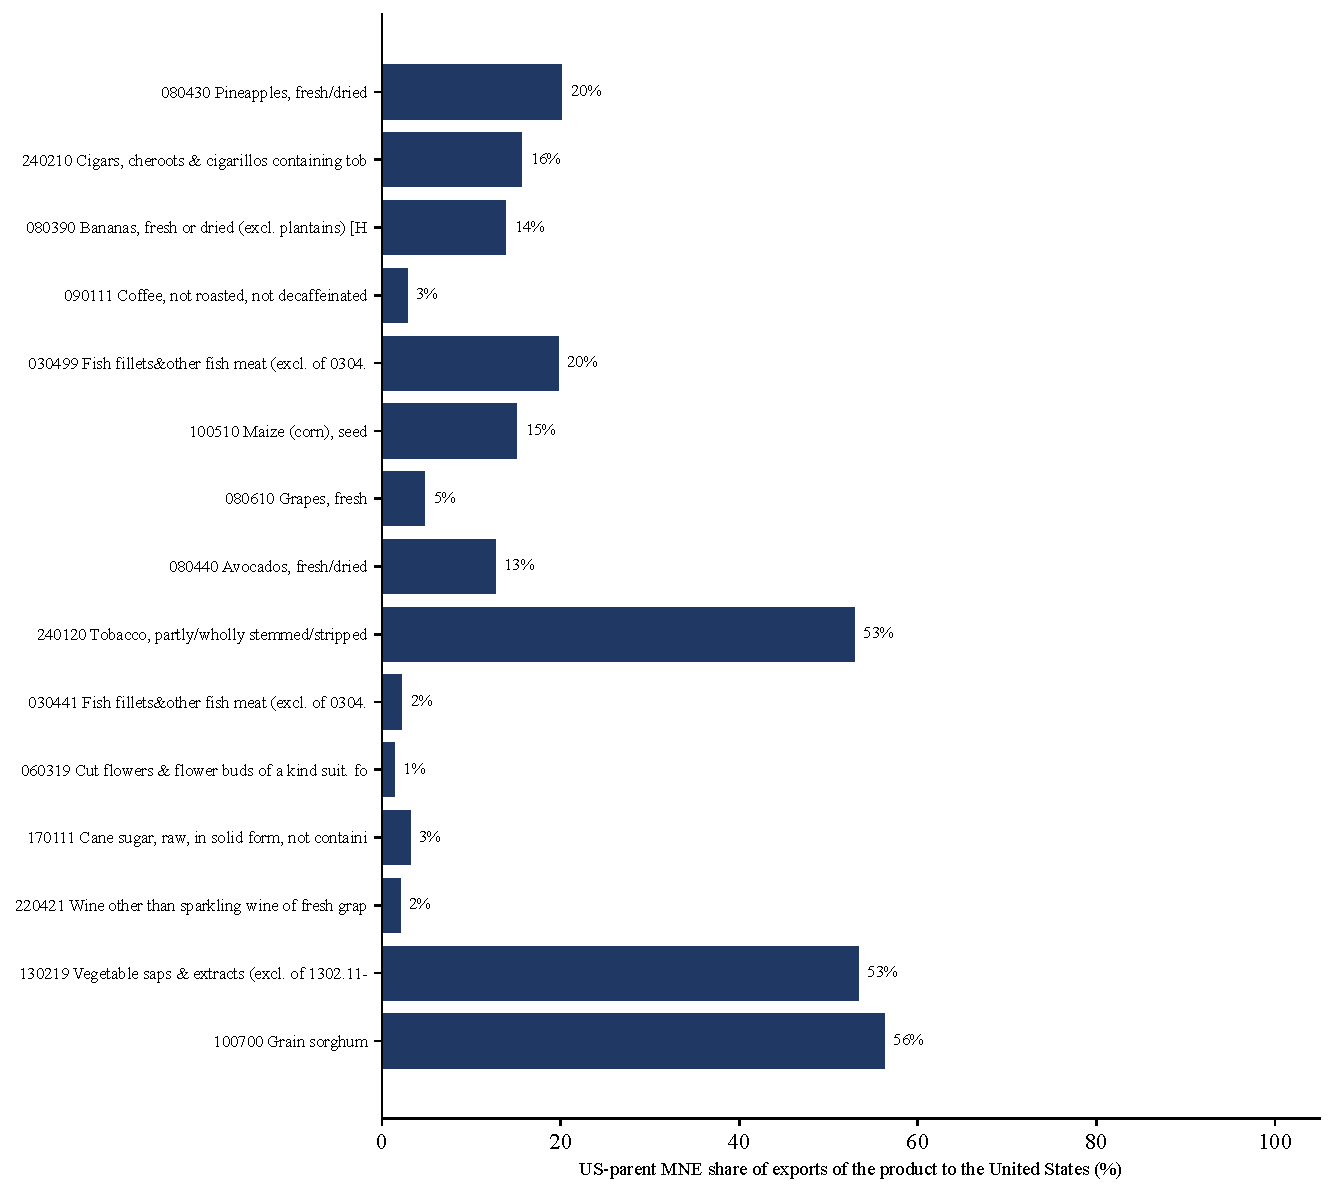
\includegraphics[width=0.95\textwidth,height=0.8\textheight,keepaspectratio]{figures/agro/fig_wp3_us_home_products.pdf}%
  \caption{Agriculture: US-Parent Share of Exports to the United States, Main Products Shipped by US-Parent Multinationals}%
  \label{fig:us_home_f_agro}%
  \par\vspace{2pt}%
  \parbox{0.92\textwidth}{\footnotesize %
  \textit{Notes:} Percent of the nine countries' exports of each product to the United States shipped by US-parent MNEs; the fifteen products with the largest US-parent exports to the United States.\\[3pt]%
  \textit{Source:} Authors' calculations based on customs data matched to Orbis and Dun \& Bradstreet.}%
  \end{figure}
% ---- Table: Agriculture: Largest Export Products to the United States, by Type of Exporter
\begin{table}[H]\centering\footnotesize%
  \caption{Agriculture: Largest Export Products to the United States, by Type of Exporter}%
  \label{tab:to_usa_prod_agro}%
  \adjustbox{max width=\textwidth, max totalheight=0.8\textheight}{\begin{tabular}{llrrrrr}
\toprule
HS6 & Description & \multicolumn{1}{p{2.0cm}}{\raggedright Exports to the USA (US\$bn/yr)} & \multicolumn{1}{p{1.8cm}}{\raggedright US-parent MNEs (\%)} & \multicolumn{1}{p{1.8cm}}{\raggedright Other foreign MNEs (\%)} & \multicolumn{1}{p{1.8cm}}{\raggedright Domestic MNEs (\%)} & \multicolumn{1}{p{1.8cm}}{\raggedright Local firms (\%)} \\
\midrule
090111 & Coffee, not roasted, not decaffeinated & 1.42 & 3 & 36 & 8 & 53 \\
060319 & Cut flowers \& flower buds of a kind suit. for... & 0.61 & 1 & 19 & 19 & 60 \\
030441 & Fish fillets\&other fish meat (excl. of 0304.1... & 0.38 & 2 & 18 & 24 & 56 \\
080610 & Grapes, fresh & 0.39 & 5 & 27 & 10 & 58 \\
240210 & Cigars, cheroots \& cigarillos containing toba... & 0.57 & 16 & 47 & 0 & 37 \\
080390 & Bananas, fresh or dried (excl. plantains) [HS... & 0.43 & 14 & 27 & 1 & 58 \\
080430 & Pineapples, fresh/dried & 0.42 & 20 & 32 & 0 & 48 \\
220421 & Wine other than sparkling wine of fresh grape... & 0.34 & 2 & 21 & 7 & 70 \\
081040 & Cranberries, bilberries \& other fruits of the... & 0.28 & 1 & 33 & 11 & 54 \\
060311 & Fresh roses & 0.25 & 2 & 19 & 8 & 70 \\
070920 & Asparagus, fresh/chilled & 0.23 & 1 & 31 & 0 & 68 \\
170111 & Cane sugar, raw, in solid form, not containin... & 0.22 & 3 & 10 & 22 & 64 \\
080300 & Bananas, incl. plantains, fresh/dried & 0.14 & 4 & 22 & 4 & 71 \\
080440 & Avocados, fresh/dried & 0.14 & 13 & 29 & 3 & 55 \\
030499 & Fish fillets\&other fish meat (excl. of 0304.1... & 0.10 & 20 & 15 & 19 & 47 \\
\bottomrule
\end{tabular}
}%
  \par\vspace{3pt}%
  \begin{minipage}{0.95\textwidth}\footnotesize %
  \textit{Notes:} Fifteen largest HS6 products exported to the United States; percent of each product's exports to the United States by type of exporter. Values are annual averages in US\$ billion.\\[3pt]%
  \textit{Source:} Authors' calculations based on customs data matched to Orbis and Dun \& Bradstreet.%
  \end{minipage}%
  \end{table}

\section{Fact 4: A Small Set of Large Multinational Groups Accounts for Most Exports}\label{sec:f4s_agro}

\subsection{Size of the Group's Global Network}
% ---- Figure: Agriculture: Foreign-Multinational Exports and Number of Parents, by Size of the Group's Global Network
\begin{figure}[H]\centering%
  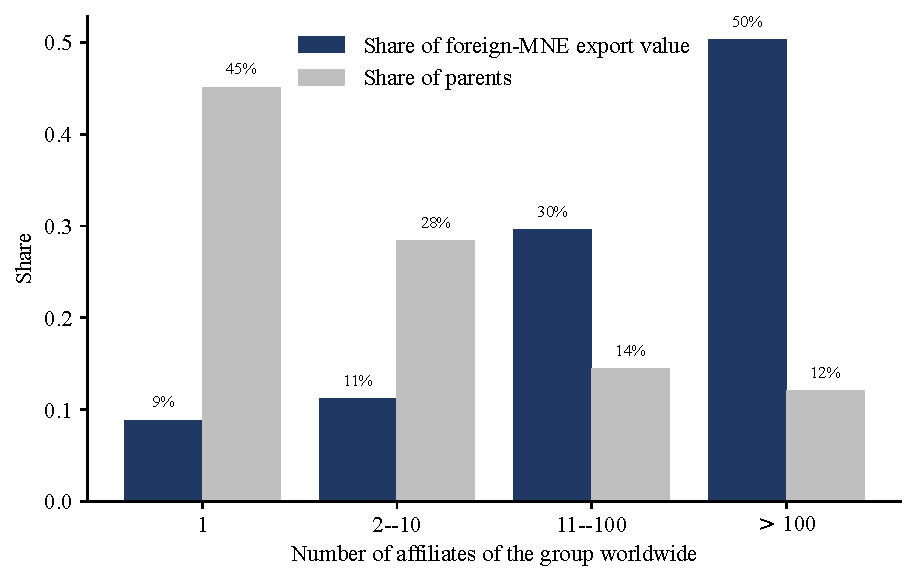
\includegraphics[width=0.7\textwidth,height=0.8\textheight,keepaspectratio]{figures/agro/fig_wp0_fig5_network.pdf}%
  \caption{Agriculture: Foreign-Multinational Exports and Number of Parents, by Size of the Group's Global Network}%
  \label{fig:net_agro}%
  \par\vspace{2pt}%
  \parbox{0.92\textwidth}{\footnotesize %
  \textit{Notes:} Shares of foreign-MNE agricultural export value and of parents, by the number of affiliates the group has worldwide.\\[3pt]%
  \textit{Source:} Authors' calculations based on customs data matched to Orbis and Dun \& Bradstreet.}%
  \end{figure}
% ---- Table: Agriculture: Foreign-Multinational Exports and Number of Parents, by Size of the Group's Global Network
\begin{table}[H]\centering\small%
  \caption{Agriculture: Foreign-Multinational Exports and Number of Parents, by Size of the Group's Global Network}%
  \label{tab:net_t_agro}%
  \adjustbox{max width=\textwidth, max totalheight=0.8\textheight}{\begin{tabular}{lrrr}
\toprule
Affiliates worldwide & Parents & Share of parents (\%) & Share of foreign-MNE export value (\%) \\
\midrule
1 & 1,436 & 45.1 & 8.9 \\
2--10 & 904 & 28.4 & 11.2 \\
11--100 & 459 & 14.4 & 29.6 \\
$>$100 & 383 & 12.0 & 50.3 \\
\midrule
All parents & 3,182 & 100 & 100 \\
\bottomrule
\end{tabular}
}%
  \par\vspace{3pt}%
  \begin{minipage}{0.95\textwidth}\footnotesize %
  \textit{Notes:} Number and share of parents, and share of foreign-MNE agricultural export value, by the number of affiliates the group has worldwide.\\[3pt]%
  \textit{Source:} Authors' calculations based on customs data matched to Orbis and Dun \& Bradstreet.%
  \end{minipage}%
  \end{table}

\subsection{Concentration within Products}
% ---- Figure: Agriculture: Export Concentration within Products: Firms and Groups
\begin{figure}[H]\centering%
  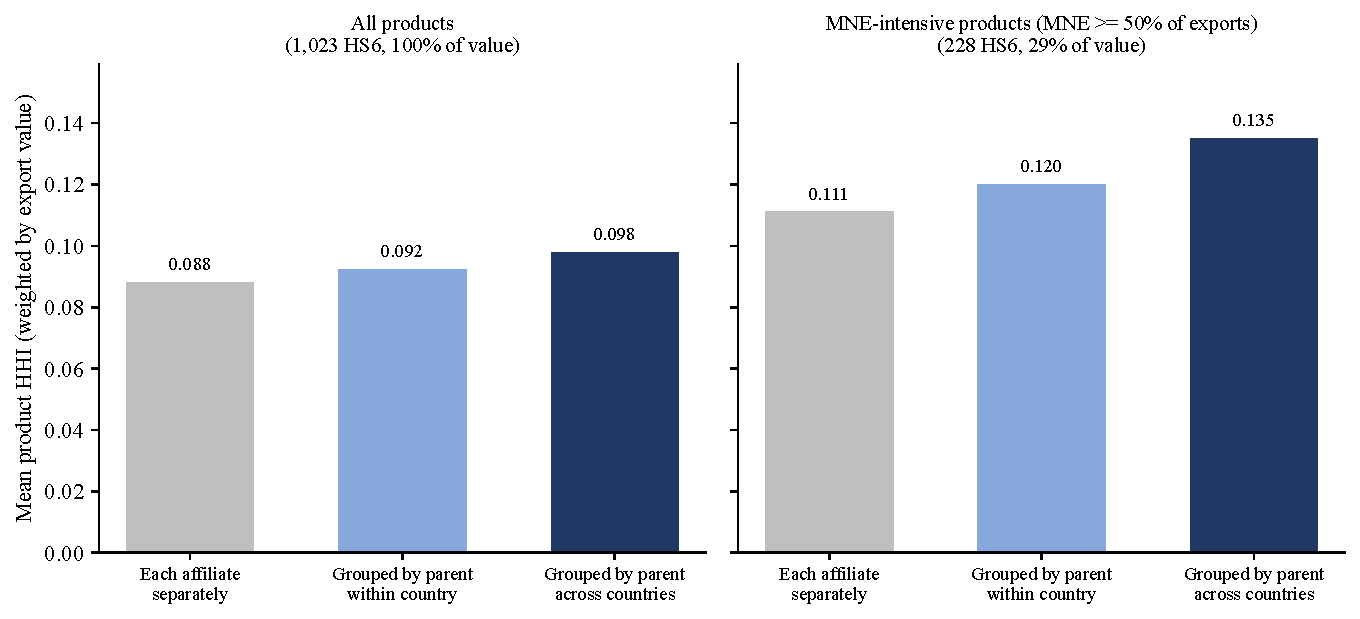
\includegraphics[width=0.9\textwidth,height=0.8\textheight,keepaspectratio]{figures/agro/fig_wp0_fig6_hhi.pdf}%
  \caption{Agriculture: Export Concentration within Products: Firms and Groups}%
  \label{fig:hhi_agro}%
  \par\vspace{2pt}%
  \parbox{0.92\textwidth}{\footnotesize %
  \textit{Notes:} Mean Herfindahl index of exporters within each HS6 product, weighted by export value, counting each affiliate separately or grouping affiliates by parent within or across countries. Right panel: products where MNEs account for at least half of exports.\\[3pt]%
  \textit{Source:} Authors' calculations based on customs data matched to Orbis and Dun \& Bradstreet.}%
  \end{figure}
% ---- Table: Agriculture: Export Concentration within Products: Firms and Groups
\begin{table}[H]\centering\small%
  \caption{Agriculture: Export Concentration within Products: Firms and Groups}%
  \label{tab:hhi_t_agro}%
  \adjustbox{max width=\textwidth, max totalheight=0.8\textheight}{\begin{tabular}{llrrr}
\toprule
Sample & Measure & Firm level & Groups within country & Groups across countries \\
\midrule
\multicolumn{5}{l}{\textit{All products: 1,023 HS6, 100\% of value}} \\
 & Mean HHI & 0.088 & 0.092 & 0.098 \\
 & Mean top-exporter share & 17.7\% & 18.1\% & 19.2\% \\
 & Effective number of exporters (1/HHI) & 18.5 & 17.3 & 16.4 \\
\multicolumn{5}{l}{\textit{MNE-intensive products (MNE $\geq$ 50\% of exports): 228 HS6, 29\% of value}} \\
 & Mean HHI & 0.111 & 0.120 & 0.135 \\
 & Mean top-exporter share & 20.7\% & 21.6\% & 24.4\% \\
 & Effective number of exporters (1/HHI) & 15.8 & 14.1 & 12.8 \\
\bottomrule
\end{tabular}
}%
  \par\vspace{3pt}%
  \begin{minipage}{0.95\textwidth}\footnotesize %
  \textit{Notes:} Means across HS6 products, weighted by export value. Firm level: each affiliate counted separately. Groups: affiliates grouped by ultimate parent within each exporting country or across countries.\\[3pt]%
  \textit{Source:} Authors' calculations based on customs data matched to Orbis and Dun \& Bradstreet.%
  \end{minipage}%
  \end{table}

\subsection{Groups and Affiliates}
% ---- Table: Agriculture: Multinational Affiliates and Groups in Origin--Destination--Product--Year Cells
\begin{table}[H]\centering\small%
  \caption{Agriculture: Multinational Affiliates and Groups in Origin--Destination--Product--Year Cells}%
  \label{tab:grp_agro}%
  \adjustbox{max width=\textwidth, max totalheight=0.8\textheight}{\begin{tabular}{lr}
\toprule
Origin-destination-product-year cells with $\geq 1$ MNE & \\
\midrule
Cells & 154,256 \\
MNE affiliates per cell (mean) & 2.17 \\
MNE groups per cell (mean) & 2.13 \\
Affiliates per group, pooled & 1.02 \\
Affiliates per group, mean weighted by export value & 1.06 \\
Cells where one group exports through $>1$ affiliate (\%) & 2.6 \\
\bottomrule
\end{tabular}
}%
  \par\vspace{3pt}%
  \begin{minipage}{0.95\textwidth}\footnotesize %
  \textit{Notes:} Cells with at least one MNE. Group: ultimate parent in Orbis or Dun \& Bradstreet (parent name when the identifier is missing).\\[3pt]%
  \textit{Source:} Authors' calculations based on customs data matched to Orbis and Dun \& Bradstreet.%
  \end{minipage}%
  \end{table}
% ---- Table: Agriculture: Multinational Presence and Exports: Affiliates and Groups
\begin{table}[H]\centering\small%
  \caption{Agriculture: Multinational Presence and Exports: Affiliates and Groups}%
  \label{tab:grp_r_agro}%
  \adjustbox{max width=\textwidth, max totalheight=0.8\textheight}{\begin{tabular}{lcccccc} \hline
 & \multicolumn{3}{c}{Origin $\times$ year, destination $\times$ year, product FE} & \multicolumn{3}{c}{Origin $\times$ dest. $\times$ product, origin $\times$ dest. $\times$ year FE} \\
 & (1) & (2) & (3) & (4) & (5) & (6) \\ \hline
\multicolumn{7}{l}{\textit{Panel A. Dependent variable: $\ln$ exports, all firms}} \\
$\ln$(\# MNE firms) & 2.1861*** &  &  & 0.8509*** &  &  \\
 & (0.0279) &  &  & (0.0190) &  &  \\
$\ln$(\# MNE groups) &  & 2.2049*** & 2.1827*** &  & 0.8525*** & 0.8528*** \\
 &  & (0.0283) & (0.0285) &  & (0.0191) & (0.0191) \\
$\ln$(affiliates per group) &  &  & 2.3343*** &  &  & 0.7524*** \\
 &  &  & (0.2073) &  &  & (0.0777) \\
\midrule
\multicolumn{7}{l}{\textit{Panel B. Dependent variable: $\ln$ exports, non-MNE firms}} \\
$\ln$(\# MNE firms) & 1.5628*** &  &  & 0.4048*** &  &  \\
 & (0.0332) &  &  & (0.0245) &  &  \\
$\ln$(\# MNE groups) &  & 1.5822*** & 1.5743*** &  & 0.4073*** & 0.4073*** \\
 &  & (0.0335) & (0.0338) &  & (0.0241) & (0.0241) \\
$\ln$(affiliates per group) &  &  & 0.9591*** &  &  & 0.2200* \\
 &  &  & (0.2648) &  &  & (0.1333) \\
\hline
Product FE & $\checkmark$ & $\checkmark$ & $\checkmark$ &  &  &  \\
Origin $\times$ year FE & $\checkmark$ & $\checkmark$ & $\checkmark$ &  &  &  \\
Destination $\times$ year FE & $\checkmark$ & $\checkmark$ & $\checkmark$ &  &  &  \\
Origin $\times$ dest.\ $\times$ product FE &  &  &  & $\checkmark$ & $\checkmark$ & $\checkmark$ \\
Origin $\times$ dest.\ $\times$ year FE &  &  &  & $\checkmark$ & $\checkmark$ & $\checkmark$ \\
Observations (Panel A) & 153,847 & 153,847 & 153,847 & 137,324 & 137,324 & 137,324 \\
Observations (Panel B) & 90,655 & 90,655 & 90,655 & 81,670 & 81,670 & 81,670 \\
\hline
\end{tabular}
}%
  \par\vspace{3pt}%
  \begin{minipage}{0.95\textwidth}\footnotesize %
  \textit{Notes:} Observations are origin--destination--HS6--year cells. Agriculture products only. Dependent variable: $\ln$ exports of the cell (Panel A) and of the non-MNE firms in the cell (Panel B). Regressors: $\ln$ number of MNE affiliates or $\ln$ number of MNE groups (distinct ultimate parents). Standard errors clustered by origin--destination pair in parentheses. *** $p<0.01$, ** $p<0.05$, * $p<0.1$.\\[3pt]%
  \textit{Source:} Authors' calculations based on customs data matched to Orbis and Dun \& Bradstreet.%
  \end{minipage}%
  \end{table}

\section{Fact 5: Multinational Presence Is Associated with Higher Exports}\label{sec:f5_agro}
% ---- Table: Agriculture: Multinational Presence and Exports
\begin{table}[H]\centering\small%
  \caption{Agriculture: Multinational Presence and Exports}%
  \label{tab:t1_agro}%
  \adjustbox{max width=\textwidth, max totalheight=0.8\textheight}{\begin{tabular}{lcccccc} \hline
 & \multicolumn{3}{c}{Intensive: $\ln$(\# MNE firms)} & \multicolumn{3}{c}{Extensive: any MNE present} \\
 & (1) & (2) & (3) & (1) & (2) & (3) \\ \hline
\multicolumn{7}{l}{\textit{Panel A. Dependent variable: $\ln$ exports, all firms}} \\
$\ln$(\# MNE firms) & 2.1821*** & 2.1861*** & 0.8509*** &  &  &  \\
 & (0.0283) & (0.0279) & (0.0190) &  &  &  \\
Any MNE present &  &  &  & 1.7857*** & 1.7863*** & 0.6860*** \\
 &  &  &  & (0.0611) & (0.0604) & (0.0232) \\
\midrule
\multicolumn{7}{l}{\textit{Panel B. Dependent variable: $\ln$ exports, non-MNE firms}} \\
$\ln$(\# MNE firms) & 1.5538*** & 1.5628*** & 0.4048*** &  &  &  \\
 & (0.0332) & (0.0332) & (0.0245) &  &  &  \\
Any MNE present &  &  &  & 1.9365*** & 1.9313*** & 0.2812*** \\
 &  &  &  & (0.0567) & (0.0554) & (0.0181) \\
\hline
Origin FE & $\checkmark$ &  &  & $\checkmark$ &  &  \\
Destination FE & $\checkmark$ &  &  & $\checkmark$ &  &  \\
Product FE & $\checkmark$ & $\checkmark$ &  & $\checkmark$ & $\checkmark$ &  \\
Year FE & $\checkmark$ &  &  & $\checkmark$ &  &  \\
Origin $\times$ year FE &  & $\checkmark$ &  &  & $\checkmark$ &  \\
Destination $\times$ year FE &  & $\checkmark$ &  &  & $\checkmark$ &  \\
Origin $\times$ dest.\ $\times$ product FE &  &  & $\checkmark$ &  &  & $\checkmark$ \\
Origin $\times$ dest.\ $\times$ year FE &  &  & $\checkmark$ &  &  & $\checkmark$ \\
Observations (Panel A) & 154,199 & 153,847 & 137,324 & 296,092 & 295,788 & 268,332 \\
Observations (Panel B) & 91,020 & 90,655 & 81,670 & 232,907 & 232,617 & 208,479 \\
\hline
\end{tabular}
}%
  \par\vspace{3pt}%
  \begin{minipage}{0.95\textwidth}\footnotesize %
  \textit{Notes:} Observations are origin--destination--HS6--year cells. Agriculture products only. Dependent variable: $\ln$ exports of the cell (Panel A) and of the non-MNE firms in the cell (Panel B). Intensive margin: $\ln$ number of MNEs, cells with at least one MNE. Extensive margin: indicator for at least one MNE. Standard errors clustered by origin--destination pair in parentheses. *** $p<0.01$, ** $p<0.05$, * $p<0.1$.\\[3pt]%
  \textit{Source:} Authors' calculations based on customs data matched to Orbis and Dun \& Bradstreet.%
  \end{minipage}%
  \end{table}
% ---- Table: Agriculture: Multinational Exports by Exporting Country and Destination Type
\begin{table}[H]\centering\small%
  \caption{Agriculture: Multinational Exports by Exporting Country and Destination Type}%
  \label{tab:pres_agro}%
  \adjustbox{max width=\textwidth, max totalheight=0.8\textheight}{\begin{tabular}{lrrrrr}
\toprule
Origin & MNE value (US\$bn/yr) & of which domestic (\%) & Foreign-MNE value (US\$bn/yr) & \multicolumn{2}{c}{\% of foreign-MNE value, by destination} \\
 & & & & parent country & other (of which: group affiliate there) \\
\midrule
ARG & 18.1 & 20.4 & 14.4 & 2.8 & 97.2 (30.6) \\
CHL & 3.6 & 38.7 & 2.2 & 12.1 & 87.9 (29.7) \\
COL & 3.0 & 33.6 & 2.0 & 4.4 & 95.6 (33.7) \\
CRI & 2.0 & 3.3 & 1.9 & 10.0 & 90.0 (45.9) \\
DOM & 0.9 & 8.8 & 0.8 & 13.7 & 86.3 (9.7) \\
PER & 3.0 & 11.7 & 2.7 & 4.7 & 95.3 (15.5) \\
PRY & 4.1 & 1.3 & 4.0 & 1.9 & 98.1 (67.8) \\
SLV & 0.3 & 0.0 & 0.3 & 9.5 & 90.5 (58.9) \\
URY & 2.7 & 15.9 & 2.3 & 2.8 & 97.2 (42.8) \\
\midrule
All & 37.8 & 19.9 & 30.7 & 4.7 & 95.3 (35.8) \\
\bottomrule
\end{tabular}
}%
  \par\vspace{3pt}%
  \begin{minipage}{0.95\textwidth}\footnotesize %
  \textit{Notes:} MNE and foreign-MNE agricultural export value by country, and the split of foreign-MNE value by destination. Parent country: exports to the country of the ultimate parent. Other: all remaining destinations; in parentheses, destinations where the group has another affiliate. Values are annual averages in US\$ billion.\\[3pt]%
  \textit{Source:} Authors' calculations based on customs data matched to Orbis and Dun \& Bradstreet.%
  \end{minipage}%
  \end{table}
% ---- Table: Agriculture: Multinational Presence and Exports: Intensive Margin, by Type of Multinational
\begin{table}[H]\centering\small%
  \caption{Agriculture: Multinational Presence and Exports: Intensive Margin, by Type of Multinational}%
  \label{tab:cnt_agro}%
  \adjustbox{max width=\textwidth, max totalheight=0.8\textheight}{\begin{tabular}{lcccccc} \hline
 & \multicolumn{2}{c}{All MNEs} & \multicolumn{2}{c}{Foreign / domestic} & \multicolumn{2}{c}{Foreign by destination, domestic} \\
 & (1) & (2) & (3) & (4) & (5) & (6) \\ \hline
\multicolumn{7}{l}{\textit{Panel A. Dependent variable: $\ln$ exports, all firms}} \\
$\ln$(\# MNE firms) & 2.1861*** & 0.8509*** &  &  &  &  \\
 & (0.0279) & (0.0190) &  &  &  &  \\
$\ln$(\# foreign MNEs) &  &  & 1.2954*** & 0.4625*** &  &  \\
 &  &  & (0.0275) & (0.0188) &  &  \\
$\ln$(\# foreign MNEs, parent-country destination) &  &  &  &  & 0.4928*** & 0.2334*** \\
 &  &  &  &  & (0.1145) & (0.0804) \\
$\ln$(\# foreign MNEs, other destinations) &  &  &  &  & 0.9569*** & 0.3804*** \\
 &  &  &  &  & (0.0754) & (0.0360) \\
$\ln$(\# domestic MNEs) &  &  & 0.5233*** & 0.2831*** & 0.4096*** & 0.1935*** \\
 &  &  & (0.0266) & (0.0234) & (0.0753) & (0.0421) \\
\midrule
\multicolumn{7}{l}{\textit{Panel B. Dependent variable: $\ln$ exports, non-MNE firms}} \\
$\ln$(\# MNE firms) & 1.5628*** & 0.4048*** &  &  &  &  \\
 & (0.0332) & (0.0245) &  &  &  &  \\
$\ln$(\# foreign MNEs) &  &  & 1.2191*** & 0.3602*** &  &  \\
 &  &  & (0.0363) & (0.0292) &  &  \\
$\ln$(\# foreign MNEs, parent-country destination) &  &  &  &  & 0.3864*** & 0.2698** \\
 &  &  &  &  & (0.1357) & (0.1255) \\
$\ln$(\# foreign MNEs, other destinations) &  &  &  &  & 1.1003*** & 0.4395*** \\
 &  &  &  &  & (0.1197) & (0.0693) \\
$\ln$(\# domestic MNEs) &  &  & 0.5676*** & 0.2461*** & 0.4367*** & 0.2032** \\
 &  &  & (0.0339) & (0.0341) & (0.1236) & (0.0759) \\
\hline
Product FE & $\checkmark$ &  & $\checkmark$ &  & $\checkmark$ &  \\
Origin $\times$ year FE & $\checkmark$ &  & $\checkmark$ &  & $\checkmark$ &  \\
Destination $\times$ year FE & $\checkmark$ &  & $\checkmark$ &  & $\checkmark$ &  \\
Origin $\times$ dest.\ $\times$ product FE &  & $\checkmark$ &  & $\checkmark$ &  & $\checkmark$ \\
Origin $\times$ dest.\ $\times$ year FE &  & $\checkmark$ &  & $\checkmark$ &  & $\checkmark$ \\
Observations (Panel A) & 153,847 & 137,324 & 25,437 & 22,002 & 1,952 & 1,604 \\
Observations (Panel B) & 90,655 & 81,670 & 22,503 & 19,535 & 1,903 & 1,567 \\
\hline
\end{tabular}
}%
  \par\vspace{3pt}%
  \begin{minipage}{0.95\textwidth}\footnotesize %
  \textit{Notes:} Observations are origin--destination--HS6--year cells. Agriculture products only. Dependent variable: $\ln$ exports of the cell (Panel A) and of the non-MNE firms in the cell (Panel B). Regressors: $\ln$ number of MNEs of each type. Columns (5)--(6) split foreign MNEs by whether the destination is the parent's country. Standard errors clustered by origin--destination pair in parentheses. *** $p<0.01$, ** $p<0.05$, * $p<0.1$.\\[3pt]%
  \textit{Source:} Authors' calculations based on customs data matched to Orbis and Dun \& Bradstreet.%
  \end{minipage}%
  \end{table}
% ---- Table: Agriculture: Multinational Presence and Exports: Extensive Margin, by Type of Multinational
\begin{table}[H]\centering\small%
  \caption{Agriculture: Multinational Presence and Exports: Extensive Margin, by Type of Multinational}%
  \label{tab:ext_agro}%
  \adjustbox{max width=\textwidth, max totalheight=0.8\textheight}{\begin{tabular}{lcccccc} \hline
 & \multicolumn{2}{c}{All MNEs} & \multicolumn{2}{c}{Foreign / domestic} & \multicolumn{2}{c}{Foreign by destination, domestic} \\
 & (1) & (2) & (3) & (4) & (5) & (6) \\ \hline
\multicolumn{7}{l}{\textit{Panel A. Dependent variable: $\ln$ exports, all firms}} \\
Any MNE present & 1.7863*** & 0.6860*** &  &  &  &  \\
 & (0.0604) & (0.0232) &  &  &  &  \\
Any foreign MNE &  &  & 1.7972*** & 0.6929*** &  &  \\
 &  &  & (0.0558) & (0.0213) &  &  \\
Any foreign MNE, parent-country destination &  &  &  &  & 1.6277*** & 0.5045*** \\
 &  &  &  &  & (0.1122) & (0.0603) \\
Any foreign MNE, other destination &  &  &  &  & 1.7886*** & 0.6904*** \\
 &  &  &  &  & (0.0563) & (0.0217) \\
Any domestic MNE &  &  & 1.6133*** & 0.5683*** & 1.5621*** & 0.5650*** \\
 &  &  & (0.0577) & (0.0237) & (0.0556) & (0.0238) \\
\midrule
\multicolumn{7}{l}{\textit{Panel B. Dependent variable: $\ln$ exports, non-MNE firms}} \\
Any MNE present & 1.9313*** & 0.2812*** &  &  &  &  \\
 & (0.0554) & (0.0181) &  &  &  &  \\
Any foreign MNE &  &  & 1.7649*** & 0.2854*** &  &  \\
 &  &  & (0.0546) & (0.0179) &  &  \\
Any foreign MNE, parent-country destination &  &  &  &  & 1.4262*** & 0.2467*** \\
 &  &  &  &  & (0.1036) & (0.0420) \\
Any foreign MNE, other destination &  &  &  &  & 1.7354*** & 0.2888*** \\
 &  &  &  &  & (0.0537) & (0.0179) \\
Any domestic MNE &  &  & 1.3082*** & 0.2610*** & 1.2541*** & 0.2590*** \\
 &  &  & (0.0539) & (0.0201) & (0.0504) & (0.0201) \\
\hline
Product FE & $\checkmark$ &  & $\checkmark$ &  & $\checkmark$ &  \\
Origin $\times$ year FE & $\checkmark$ &  & $\checkmark$ &  & $\checkmark$ &  \\
Destination $\times$ year FE & $\checkmark$ &  & $\checkmark$ &  & $\checkmark$ &  \\
Origin $\times$ dest.\ $\times$ product FE &  & $\checkmark$ &  & $\checkmark$ &  & $\checkmark$ \\
Origin $\times$ dest.\ $\times$ year FE &  & $\checkmark$ &  & $\checkmark$ &  & $\checkmark$ \\
Observations (Panel A) & 295,788 & 268,332 & 295,788 & 268,332 & 295,788 & 268,332 \\
Observations (Panel B) & 232,617 & 208,479 & 232,617 & 208,479 & 232,617 & 208,479 \\
\hline
\end{tabular}
}%
  \par\vspace{3pt}%
  \begin{minipage}{0.95\textwidth}\footnotesize %
  \textit{Notes:} Observations are origin--destination--HS6--year cells. Agriculture products only. Dependent variable: $\ln$ exports of the cell (Panel A) and of the non-MNE firms in the cell (Panel B). Regressors: indicators for at least one MNE of each type. Columns (5)--(6) split foreign MNEs by whether the destination is the parent's country. Standard errors clustered by origin--destination pair in parentheses. *** $p<0.01$, ** $p<0.05$, * $p<0.1$.\\[3pt]%
  \textit{Source:} Authors' calculations based on customs data matched to Orbis and Dun \& Bradstreet.%
  \end{minipage}%
  \end{table}

\section{Fact 6: Distance Is a Weaker Barrier for Multinationals}\label{sec:f6_agro}
% ---- Table: Agriculture: Distance and Firm Exports: Multinationals by Presence at the Destination
\begin{table}[H]\centering\small%
  \caption{Agriculture: Distance and Firm Exports: Multinationals by Presence at the Destination}%
  \label{tab:t2_agro}%
  \adjustbox{max width=\textwidth, max totalheight=0.8\textheight}{\begin{tabular}{lcccc} \hline
Dep.\ var.: $\ln$ exports & (1) & (2) & (3) & (4) \\ \hline
$\ln$ distance & -0.2118*** & -0.2269*** & -0.2078*** & -0.2224*** \\
 & (0.0748) & (0.0712) & (0.0745) & (0.0708) \\
$\ln$ distance $\times$ MNE & 0.0326*** & 0.0318*** &  &  \\
 & (0.0031) & (0.0031) &  &  \\
$\ln$ distance $\times$ MNE, present at destination &  &  & 0.0890*** & 0.0875*** \\
 &  &  & (0.0070) & (0.0069) \\
$\ln$ distance $\times$ MNE, not present at destination &  &  & 0.0228*** & 0.0221*** \\
 &  &  & (0.0032) & (0.0032) \\
\hline
Origin FE & $\checkmark$ &  & $\checkmark$ &  \\
Destination FE & $\checkmark$ &  & $\checkmark$ &  \\
Year FE & $\checkmark$ &  & $\checkmark$ &  \\
Origin $\times$ year FE &  & $\checkmark$ &  & $\checkmark$ \\
Destination $\times$ year FE &  & $\checkmark$ &  & $\checkmark$ \\
Product FE & $\checkmark$ & $\checkmark$ & $\checkmark$ & $\checkmark$ \\
\hline
Observations & 1,045,009 & 1,044,787 & 1,045,009 & 1,044,787 \\
\hline
\end{tabular}
}%
  \par\vspace{3pt}%
  \begin{minipage}{0.95\textwidth}\footnotesize %
  \textit{Notes:} Observations are firm--destination--HS6--year cells. Agriculture products only. Dependent variable: $\ln$ exports. Non-MNE firms are the omitted group. Present: the group has an affiliate in the destination or the destination is the parent's country. Standard errors clustered by origin--destination pair in parentheses. *** $p<0.01$, ** $p<0.05$, * $p<0.1$.\\[3pt]%
  \textit{Source:} Authors' calculations based on customs data matched to Orbis and Dun \& Bradstreet.%
  \end{minipage}%
  \end{table}
% ---- Table: Agriculture: Distance and Firm Exports: Foreign and Domestic Multinationals
\begin{table}[H]\centering\small%
  \caption{Agriculture: Distance and Firm Exports: Foreign and Domestic Multinationals}%
  \label{tab:dist_agro}%
  \adjustbox{max width=\textwidth, max totalheight=0.8\textheight}{\begin{tabular}{lcccc} \hline
Dep.\ var.: $\ln$ exports & (1) & (2) & (3) & (4) \\ \hline
$\ln$ distance & -0.2135*** & -0.2285*** & -0.2130*** & -0.2280*** \\
 & (0.0748) & (0.0711) & (0.0748) & (0.0711) \\
$\ln$ distance $\times$ foreign MNE & 0.0366*** & 0.0358*** &  &  \\
 & (0.0034) & (0.0034) &  &  \\
$\ln$ distance $\times$ foreign MNE, parent-country destination &  &  & 0.0610*** & 0.0590*** \\
 &  &  & (0.0165) & (0.0165) \\
$\ln$ distance $\times$ foreign MNE, other destination &  &  & 0.0359*** & 0.0351*** \\
 &  &  & (0.0035) & (0.0034) \\
$\ln$ distance $\times$ domestic MNE & 0.0187*** & 0.0182*** & 0.0187*** & 0.0182*** \\
 & (0.0046) & (0.0046) & (0.0046) & (0.0046) \\
\hline
Origin FE & $\checkmark$ &  & $\checkmark$ &  \\
Destination FE & $\checkmark$ &  & $\checkmark$ &  \\
Year FE & $\checkmark$ &  & $\checkmark$ &  \\
Origin $\times$ year FE &  & $\checkmark$ &  & $\checkmark$ \\
Destination $\times$ year FE &  & $\checkmark$ &  & $\checkmark$ \\
Product FE & $\checkmark$ & $\checkmark$ & $\checkmark$ & $\checkmark$ \\
\hline
Observations & 1,045,009 & 1,044,787 & 1,045,009 & 1,044,787 \\
\hline
\end{tabular}
}%
  \par\vspace{3pt}%
  \begin{minipage}{0.95\textwidth}\footnotesize %
  \textit{Notes:} Observations are firm--destination--HS6--year cells. Agriculture products only. Dependent variable: $\ln$ exports. Non-MNE firms are the omitted group. Columns (3)--(4) split foreign MNEs by whether the destination is the parent's country. Standard errors clustered by origin--destination pair in parentheses. *** $p<0.01$, ** $p<0.05$, * $p<0.1$.\\[3pt]%
  \textit{Source:} Authors' calculations based on customs data matched to Orbis and Dun \& Bradstreet.%
  \end{minipage}%
  \end{table}

\section{Products}\label{sec:hs6_agro}
% ---- Figure: Agriculture: Ownership of the Twenty Largest Export Products
\begin{figure}[H]\centering%
  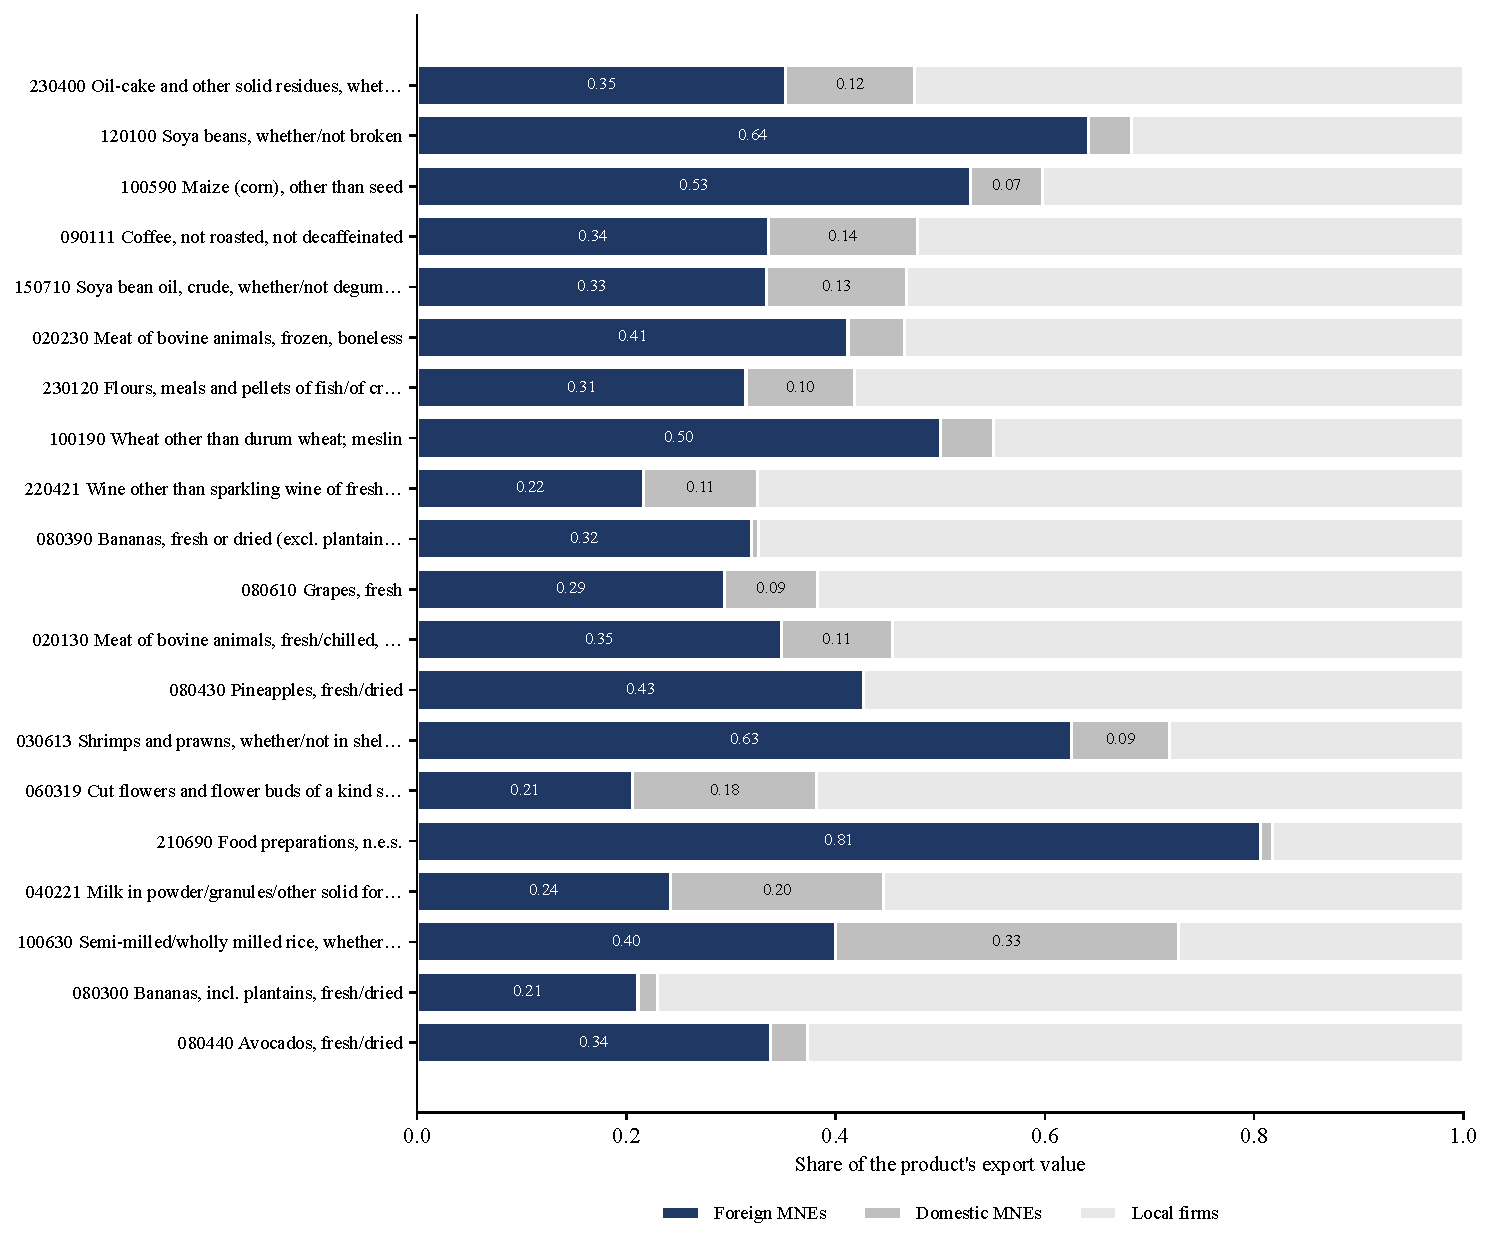
\includegraphics[width=1.0\textwidth,height=0.8\textheight,keepaspectratio]{figures/agro/fig_wp1f_top20_hs6_stacked.pdf}%
  \caption{Agriculture: Ownership of the Twenty Largest Export Products}%
  \label{fig:hs_st_agro}%
  \par\vspace{2pt}%
  \parbox{0.92\textwidth}{\footnotesize %
  \textit{Notes:} Shares of each product's export value. Twenty largest HS6 products by export value.\\[3pt]%
  \textit{Source:} Authors' calculations based on customs data matched to Orbis and Dun \& Bradstreet.}%
  \end{figure}
% ---- Figure: Agriculture: Ownership of the Twenty Largest Export Products, by Parent Country
\begin{figure}[H]\centering%
  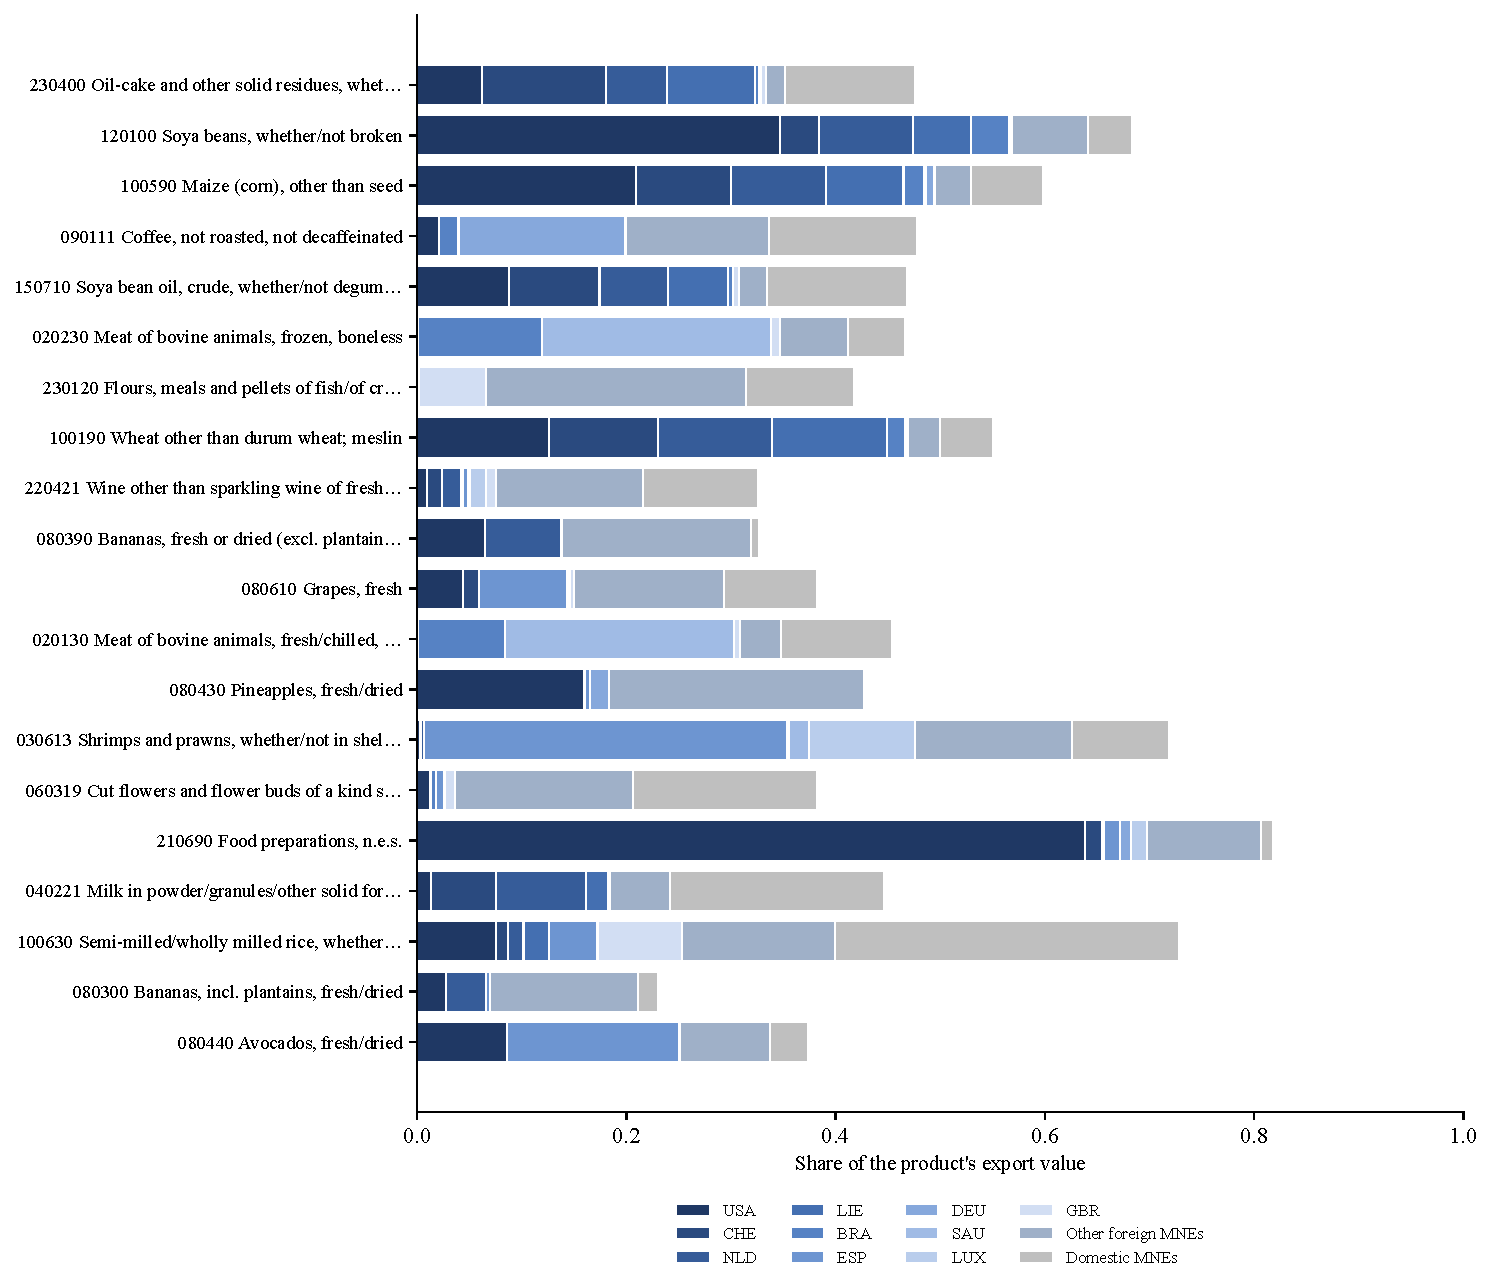
\includegraphics[width=1.0\textwidth,height=0.8\textheight,keepaspectratio]{figures/agro/fig_wp1f_top20_hs6_by_parent.pdf}%
  \caption{Agriculture: Ownership of the Twenty Largest Export Products, by Parent Country}%
  \label{fig:hs_par_agro}%
  \par\vspace{2pt}%
  \parbox{0.92\textwidth}{\footnotesize %
  \textit{Notes:} Shares of each product's export value. Foreign-MNE share split by country of the ultimate parent; the unfilled part of each bar is local firms.\\[3pt]%
  \textit{Source:} Authors' calculations based on customs data matched to Orbis and Dun \& Bradstreet.}%
  \end{figure}
% ---- Figure: Agriculture: Distribution of Export Value by Product-Level Foreign-Multinational Share
\begin{figure}[H]\centering%
  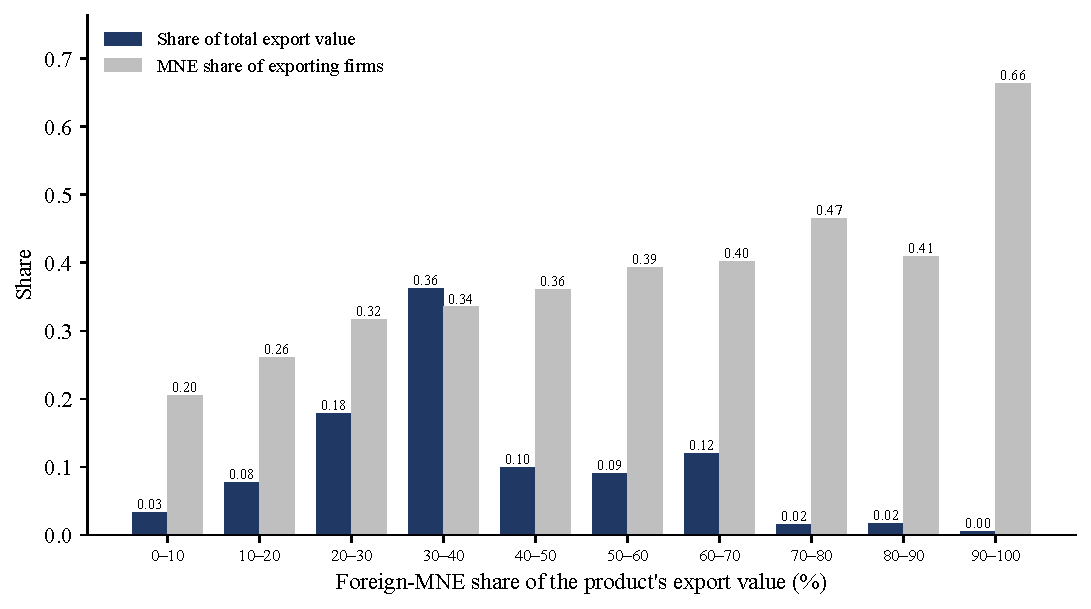
\includegraphics[width=0.85\textwidth,height=0.8\textheight,keepaspectratio]{figures/agro/fig_wp1f_foreign_share_distribution.pdf}%
  \caption{Agriculture: Distribution of Export Value by Product-Level Foreign-Multinational Share}%
  \label{fig:hs_dist_agro}%
  \par\vspace{2pt}%
  \parbox{0.92\textwidth}{\footnotesize %
  \textit{Notes:} Share of agricultural export value and MNE share of exporting firms, by the foreign-MNE share of each HS6 product's export value.\\[3pt]%
  \textit{Source:} Authors' calculations based on customs data matched to Orbis and Dun \& Bradstreet.}%
  \end{figure}
% ---- Table: Agriculture: Distribution of Export Value by Product-Level Foreign-Multinational Share
\begin{table}[H]\centering\small%
  \caption{Agriculture: Distribution of Export Value by Product-Level Foreign-Multinational Share}%
  \label{tab:hs_dist_t_agro}%
  \adjustbox{max width=\textwidth, max totalheight=0.8\textheight}{\begin{tabular}{lrrr}
\toprule
Foreign share bin (\%) & Share of value & MNE share of exporting firms & HS6 products \\
\midrule
0--10 & 0.034 & 0.205 & 349 \\
10--20 & 0.077 & 0.261 & 159 \\
20--30 & 0.179 & 0.316 & 134 \\
30--40 & 0.363 & 0.335 & 103 \\
40--50 & 0.099 & 0.361 & 60 \\
50--60 & 0.091 & 0.393 & 53 \\
60--70 & 0.119 & 0.402 & 49 \\
70--80 & 0.016 & 0.466 & 37 \\
80--90 & 0.018 & 0.409 & 30 \\
90--100 & 0.005 & 0.664 & 49 \\
\bottomrule
\end{tabular}
}%
  \par\vspace{3pt}%
  \begin{minipage}{0.95\textwidth}\footnotesize %
  \textit{Notes:} Share of agricultural export value and MNE share of exporting firms, by the foreign-MNE share of each HS6 product's export value. MNE share of exporting firms: MNE firm--destination--product--year observations over all observations in the bin.\\[3pt]%
  \textit{Source:} Authors' calculations based on customs data matched to Orbis and Dun \& Bradstreet.%
  \end{minipage}%
  \end{table}
% ---- Figure: Agriculture: Concentration of Exports across Products
\begin{figure}[H]\centering%
  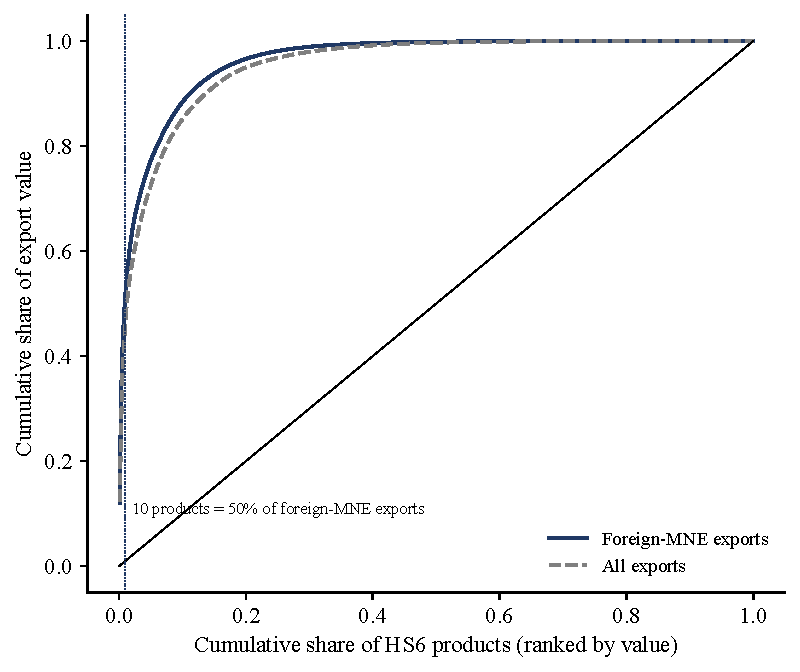
\includegraphics[width=0.6\textwidth,height=0.8\textheight,keepaspectratio]{figures/agro/fig_wp1f_lorenz_foreign.pdf}%
  \caption{Agriculture: Concentration of Exports across Products}%
  \label{fig:hs_lor_agro}%
  \par\vspace{2pt}%
  \parbox{0.92\textwidth}{\footnotesize %
  \textit{Notes:} Cumulative share of export value against the cumulative share of HS6 products, ranked by value, for foreign-MNE exports and for all exports.\\[3pt]%
  \textit{Source:} Authors' calculations based on customs data matched to Orbis and Dun \& Bradstreet.}%
  \end{figure}
% ---- Table: Agriculture: Exports and Multinational Shares, by HS Section
\begin{table}[H]\centering\footnotesize%
  \caption{Agriculture: Exports and Multinational Shares, by HS Section}%
  \label{tab:hs_sec_agro}%
  \adjustbox{max width=\textwidth, max totalheight=0.8\textheight}{\begin{tabular}{@{}p{7.2cm} r r r r l@{}}
\toprule
HS section & US\$bn/yr & Foreign (\%) & Domestic (\%) & Local (\%) & Leading parent \\
\midrule
II Vegetable products & 33.5 & 42 & 7 & 51 & USA (0.33) \\
IV Prepared foodstuffs, beverages, tobacco & 25.9 & 37 & 10 & 53 & USA (0.21) \\
I Live animals; animal products & 12.5 & 34 & 14 & 51 & SAU (0.19) \\
III Fats and oils & 6.9 & 31 & 10 & 59 & CHE (0.26) \\
\midrule
All sections & 78.9 & 38 & 9 & 52 & \\
\bottomrule
\end{tabular}
}%
  \par\vspace{3pt}%
  \begin{minipage}{0.95\textwidth}\footnotesize %
  \textit{Notes:} Foreign, domestic and local: percent of each section's export value. Leading parent: largest parent country and its share of the section's foreign-MNE exports. Values are annual averages in US\$ billion.\\[3pt]%
  \textit{Source:} Authors' calculations based on customs data matched to Orbis and Dun \& Bradstreet.%
  \end{minipage}%
  \end{table}
% ---- Table: Agriculture: Thirty Largest Export Products
\begin{table}[H]\centering\footnotesize%
  \caption{Agriculture: Thirty Largest Export Products}%
  \label{tab:hs_by_value_agro}%
  \adjustbox{max width=\textwidth, max totalheight=0.8\textheight}{\begin{tabular}{@{}l p{6.4cm} r r r r l@{}}
\toprule
HS6 & Description & US\$bn/yr & Foreign (\%) & Domestic (\%) & Local (\%) & Leading parent \\
\midrule
230400 & Oil-cake and other solid residues, whether/\allowbreak{}not ground/\allowbreak{}in pellets, from extraction of soyabean ... & 10.8 & 35 & 12 & 52 & CHE (0.34) \\
120100 & Soya beans, whether/\allowbreak{}not broken & 6.2 & 64 & 4 & 32 & USA (0.54) \\
100590 & Maize (corn), other than seed & 4.8 & 53 & 7 & 40 & USA (0.40) \\
090111 & Coffee, not roasted, not decaffeinated & 3.7 & 34 & 14 & 52 & DEU (0.47) \\
150710 & Soya bean oil, crude, whether/\allowbreak{}not degummed, not chemically modified & 4.3 & 33 & 13 & 53 & USA (0.26) \\
020230 & Meat of bovine animals, frozen, boneless & 2.1 & 41 & 5 & 53 & SAU (0.53) \\
230120 & Flours, meals and pellets of fish/\allowbreak{}of crustaceans, molluscs/\allowbreak{}other aquatic invertebrates & 1.7 & 31 & 10 & 58 & BMU (0.38) \\
100190 & Wheat other than durum wheat; meslin & 1.9 & 50 & 5 & 45 & USA (0.25) \\
220421 & Wine other than sparkling wine of fresh grapes, incl. fortified; grape must with fermentation ... & 1.4 & 22 & 11 & 67 & FRA (0.25) \\
080390 & Bananas, fresh or dried (excl. plantains) [HS2012 code] & 1.4 & 32 & 1 & 67 & JOR (0.38) \\
080610 & Grapes, fresh & 1.1 & 29 & 9 & 62 & ESP (0.29) \\
020130 & Meat of bovine animals, fresh/\allowbreak{}chilled, boneless & 1.4 & 35 & 11 & 55 & SAU (0.63) \\
080430 & Pineapples, fresh/\allowbreak{}dried & 0.9 & 43 & 0 & 57 & JOR (0.47) \\
030613 & Shrimps and prawns, whether/\allowbreak{}not in shell, frozen & 0.9 & 63 & 9 & 28 & ESP (0.55) \\
060319 & Cut flowers and flower buds of a kind suit. for bouquets/\allowbreak{}ornamental purposes(excl. of 0603.11-... & 0.7 & 21 & 18 & 62 & ARG (0.30) \\
210690 & Food preparations, n.e.s. & 0.7 & 81 & 1 & 18 & USA (0.79) \\
040221 & Milk in powder/\allowbreak{}granules/\allowbreak{}other solid form, unsweetened, fat content by weight >1.5\% & 0.8 & 24 & 20 & 55 & NLD (0.36) \\
100630 & Semi-milled/\allowbreak{}wholly milled rice, whether/\allowbreak{}not polished/\allowbreak{}glazed & 0.6 & 40 & 33 & 27 & CHN (0.25) \\
080300 & Bananas, incl. plantains, fresh/\allowbreak{}dried & 0.6 & 21 & 2 & 77 & JOR (0.34) \\
080440 & Avocados, fresh/\allowbreak{}dried & 0.5 & 34 & 4 & 63 & ESP (0.49) \\
081040 & Cranberries, bilberries and other fruits of the genus Vaccinium, fresh & 0.5 & 37 & 11 & 52 & ESP (0.39) \\
030441 & Fish filletsandother fish meat (excl. of 0304.11-0304.12, whether/\allowbreak{}not minced), fresh/\allowbreak{}chilled [... & 0.4 & 20 & 24 & 56 & JPN (0.50) \\
080810 & Apples, fresh & 0.4 & 25 & 14 & 61 & USA (0.39) \\
100300 & Barley & 0.6 & 55 & 4 & 41 & USA (0.37) \\
240210 & Cigars, cheroots and cigarillos containing tobacco & 0.6 & 62 & 0 & 38 & HKG (0.40) \\
151211 & Sunflower seed/\allowbreak{}safflower oil, crude & 0.6 & 19 & 2 & 79 & NLD (0.69) \\
230990 & Preparations of a kind used in animal feeding other than dog/\allowbreak{}cat food put up for RS & 0.5 & 57 & 3 & 40 & USA (0.44) \\
170199 & Cane/\allowbreak{}beet sugar and chemically pure sucrose, in solid form, not containing added flavouring/\allowbreak{}co... & 0.4 & 19 & 0 & 81 & USA (0.95) \\
150420 & Fats and oils and their fractions, of fish, other than liver oils, whether/\allowbreak{}not refined but not... & 0.4 & 23 & 12 & 65 & BMU (0.37) \\
110710 & Malt, not roasted & 0.5 & 71 & 0 & 29 & LUX (0.86) \\
\bottomrule
\end{tabular}
}%
  \par\vspace{3pt}%
  \begin{minipage}{0.95\textwidth}\footnotesize %
  \textit{Notes:} Thirty largest HS6 products by export value. Foreign, domestic and local: percent of the product's export value. Leading parent: largest parent country and its share of the product's foreign-MNE exports. Values are annual averages in US\$ billion.\\[3pt]%
  \textit{Source:} Authors' calculations based on customs data matched to Orbis and Dun \& Bradstreet.%
  \end{minipage}%
  \end{table}
% ---- Table: Agriculture: Thirty Largest Export Products of Foreign Multinationals
\begin{table}[H]\centering\footnotesize%
  \caption{Agriculture: Thirty Largest Export Products of Foreign Multinationals}%
  \label{tab:hs_by_foreign_value_agro}%
  \adjustbox{max width=\textwidth, max totalheight=0.8\textheight}{\begin{tabular}{@{}l p{6.4cm} r r r r l@{}}
\toprule
HS6 & Description & US\$bn/yr & Foreign (\%) & Domestic (\%) & Local (\%) & Leading parent \\
\midrule
120100 & Soya beans, whether/\allowbreak{}not broken & 6.2 & 64 & 4 & 32 & USA (0.54) \\
230400 & Oil-cake and other solid residues, whether/\allowbreak{}not ground/\allowbreak{}in pellets, from extraction of soyabean ... & 10.8 & 35 & 12 & 52 & CHE (0.34) \\
100590 & Maize (corn), other than seed & 4.8 & 53 & 7 & 40 & USA (0.40) \\
090111 & Coffee, not roasted, not decaffeinated & 3.7 & 34 & 14 & 52 & DEU (0.47) \\
150710 & Soya bean oil, crude, whether/\allowbreak{}not degummed, not chemically modified & 4.3 & 33 & 13 & 53 & USA (0.26) \\
100190 & Wheat other than durum wheat; meslin & 1.9 & 50 & 5 & 45 & USA (0.25) \\
020230 & Meat of bovine animals, frozen, boneless & 2.1 & 41 & 5 & 53 & SAU (0.53) \\
210690 & Food preparations, n.e.s. & 0.7 & 81 & 1 & 18 & USA (0.79) \\
230120 & Flours, meals and pellets of fish/\allowbreak{}of crustaceans, molluscs/\allowbreak{}other aquatic invertebrates & 1.7 & 31 & 10 & 58 & BMU (0.38) \\
030613 & Shrimps and prawns, whether/\allowbreak{}not in shell, frozen & 0.9 & 63 & 9 & 28 & ESP (0.55) \\
080390 & Bananas, fresh or dried (excl. plantains) [HS2012 code] & 1.4 & 32 & 1 & 67 & JOR (0.38) \\
020130 & Meat of bovine animals, fresh/\allowbreak{}chilled, boneless & 1.4 & 35 & 11 & 55 & SAU (0.63) \\
080610 & Grapes, fresh & 1.1 & 29 & 9 & 62 & ESP (0.29) \\
080430 & Pineapples, fresh/\allowbreak{}dried & 0.9 & 43 & 0 & 57 & JOR (0.47) \\
220421 & Wine other than sparkling wine of fresh grapes, incl. fortified; grape must with fermentation ... & 1.4 & 22 & 11 & 67 & FRA (0.25) \\
240210 & Cigars, cheroots and cigarillos containing tobacco & 0.6 & 62 & 0 & 38 & HKG (0.40) \\
110710 & Malt, not roasted & 0.5 & 71 & 0 & 29 & LUX (0.86) \\
230990 & Preparations of a kind used in animal feeding other than dog/\allowbreak{}cat food put up for RS & 0.5 & 57 & 3 & 40 & USA (0.44) \\
100300 & Barley & 0.6 & 55 & 4 & 41 & USA (0.37) \\
100630 & Semi-milled/\allowbreak{}wholly milled rice, whether/\allowbreak{}not polished/\allowbreak{}glazed & 0.6 & 40 & 33 & 27 & CHN (0.25) \\
120190 & Soya beans, whether/\allowbreak{}not broken [HS 2007 line 120100] & 0.4 & 69 & 0 & 31 & USA (0.50) \\
081040 & Cranberries, bilberries and other fruits of the genus Vaccinium, fresh & 0.5 & 37 & 11 & 52 & ESP (0.39) \\
202300 & HS 202300 (no description available) & 0.3 & 68 & 7 & 25 & BRA (0.37) \\
080440 & Avocados, fresh/\allowbreak{}dried & 0.5 & 34 & 4 & 63 & ESP (0.49) \\
040221 & Milk in powder/\allowbreak{}granules/\allowbreak{}other solid form, unsweetened, fat content by weight >1.5\% & 0.8 & 24 & 20 & 55 & NLD (0.36) \\
060319 & Cut flowers and flower buds of a kind suit. for bouquets/\allowbreak{}ornamental purposes(excl. of 0603.11-... & 0.7 & 21 & 18 & 62 & ARG (0.30) \\
100700 & Grain sorghum & 0.2 & 74 & 1 & 25 & USA (0.78) \\
070920 & Asparagus, fresh/\allowbreak{}chilled & 0.4 & 41 & 0 & 59 & PAN (0.53) \\
100199 & Wheat other than durum wheat; meslin [HS 2007 line 100190] & 0.3 & 62 & 2 & 36 & NLD (0.32) \\
240120 & Tobacco, partly/\allowbreak{}wholly stemmed/\allowbreak{}stripped & 0.4 & 44 & 0 & 56 & USA (0.74) \\
\bottomrule
\end{tabular}
}%
  \par\vspace{3pt}%
  \begin{minipage}{0.95\textwidth}\footnotesize %
  \textit{Notes:} Thirty largest HS6 products by foreign-MNE export value. Foreign, domestic and local: percent of the product's export value. Leading parent: largest parent country and its share of the product's foreign-MNE exports. Values are annual averages in US\$ billion.\\[3pt]%
  \textit{Source:} Authors' calculations based on customs data matched to Orbis and Dun \& Bradstreet.%
  \end{minipage}%
  \end{table}
% ---- Table: Agriculture: Products with the Highest Foreign-Multinational Share
\begin{table}[H]\centering\footnotesize%
  \caption{Agriculture: Products with the Highest Foreign-Multinational Share}%
  \label{tab:hs_by_foreign_share_agro}%
  \adjustbox{max width=\textwidth, max totalheight=0.8\textheight}{\begin{tabular}{@{}l p{6.4cm} r r r r l@{}}
\toprule
HS6 & Description & US\$bn/yr & Foreign (\%) & Domestic (\%) & Local (\%) & Leading parent \\
\midrule
190110 & Preparations for infant use, put up for RS & 0.1 & 92 & 3 & 5 & CHE (0.63) \\
200410 & Potatoes, prepared/\allowbreak{}preserved othw. than by vinegar/\allowbreak{}acetic acid, frozen, other than products of... & 0.2 & 85 & 0 & 14 & CAN (0.98) \\
040291 & Milk and cream, concentrated (excl. in powder), unsweetened & 0.1 & 85 & 0 & 15 & ROU (0.99) \\
230910 & Dog/\allowbreak{}cat food, put up for RS & 0.2 & 81 & 5 & 13 & USA (0.60) \\
210690 & Food preparations, n.e.s. & 0.7 & 81 & 1 & 18 & USA (0.79) \\
200949 & Pineapple juice (excl. of 2009.41), unfermented and not containing added spirit, whether/\allowbreak{}not c... & 0.1 & 79 & 0 & 20 & PAN (0.69) \\
220300 & Beer made from malt & 0.1 & 78 & 0 & 22 & LUX (0.80) \\
200941 & Pineapple juice, of a Brix value not >20, unfermented and not containing added spirit, whether... & 0.1 & 75 & 0 & 25 & PAN (0.51) \\
100700 & Grain sorghum & 0.2 & 74 & 1 & 25 & USA (0.78) \\
220290 & Non-alcoholic beverages other than waters of 2202.10 (not incl. fruit/\allowbreak{}vegetable juices of 20.0... & 0.1 & 73 & 3 & 24 & PAN (0.71) \\
110710 & Malt, not roasted & 0.5 & 71 & 0 & 29 & LUX (0.86) \\
200560 & Asparagus, preserved/\allowbreak{}preserved othw. than by vinegar/\allowbreak{}acetic acid, not frozen, other than produ... & 0.1 & 71 & 0 & 29 & ESP (0.47) \\
120190 & Soya beans, whether/\allowbreak{}not broken [HS 2007 line 120100] & 0.4 & 69 & 0 & 31 & USA (0.50) \\
200290 & Tomatoes, prepared/\allowbreak{}preserved othw. than by vinegar/\allowbreak{}acetic acid, other than whole/\allowbreak{}in pieces & 0.1 & 68 & 0 & 32 & DEU (0.48) \\
202300 & HS 202300 (no description available) & 0.3 & 68 & 7 & 25 & BRA (0.37) \\
120991 & Vegetable seeds, of a kind used for sowing & 0.1 & 67 & 1 & 32 & DEU (0.54) \\
160414 & Tunas, skipjack and bonito (Sarda spp.), prepared/\allowbreak{}preserved, whole/\allowbreak{}in pieces (excl. minced) & 0.1 & 67 & 0 & 33 & ITA (0.97) \\
220840 & Rum and tafia & 0.1 & 66 & 2 & 32 & GBR (0.76) \\
120100 & Soya beans, whether/\allowbreak{}not broken & 6.2 & 64 & 4 & 32 & USA (0.54) \\
200190 & Vegetables, fruit, nuts and other edible parts of plants (excl. cucumbers and gherkins), prepa... & 0.1 & 64 & 2 & 34 & PAN (0.51) \\
151790 & Edible mixtures/\allowbreak{}preparations of animal/\allowbreak{}vegetable fats/\allowbreak{}oils/\allowbreak{}fractions of different fats/\allowbreak{}oils of... & 0.2 & 64 & 5 & 31 & SWE (0.49) \\
210390 & Sauces and preparations therefor, n.e.s.; mixed condiments and mixed seasonings, n.e.s. & 0.2 & 63 & 1 & 35 & USA (0.36) \\
030613 & Shrimps and prawns, whether/\allowbreak{}not in shell, frozen & 0.9 & 63 & 9 & 28 & ESP (0.55) \\
240210 & Cigars, cheroots and cigarillos containing tobacco & 0.6 & 62 & 0 & 38 & HKG (0.40) \\
100199 & Wheat other than durum wheat; meslin [HS 2007 line 100190] & 0.3 & 62 & 2 & 36 & NLD (0.32) \\
190190 & Malt extract; food preparations of flour/\allowbreak{}groats/\allowbreak{}meal/\allowbreak{}starch/\allowbreak{}malt extact,not containing cocoa/\allowbreak{}c... & 0.1 & 62 & 5 & 34 & CHE (0.50) \\
200979 & Apple juice (excl. of 2009.71), unfermented and not containing added spirit, whether/\allowbreak{}not conta... & 0.1 & 62 & 1 & 37 & DEU (0.75) \\
201300 & HS 201300 (no description available) & 0.1 & 60 & 13 & 27 & BRA (0.44) \\
100510 & Maize (corn), seed & 0.2 & 60 & 3 & 37 & DEU (0.57) \\
120600 & Sunflower seeds, whether/\allowbreak{}not broken & 0.1 & 58 & 4 & 38 & USA (0.31) \\
\bottomrule
\end{tabular}
}%
  \par\vspace{3pt}%
  \begin{minipage}{0.95\textwidth}\footnotesize %
  \textit{Notes:} HS6 products with exports of at least US\$500 million over the period, ranked by foreign-MNE share. Foreign, domestic and local: percent of the product's export value. Leading parent: largest parent country and its share of the product's foreign-MNE exports. Values are annual averages in US\$ billion.\\[3pt]%
  \textit{Source:} Authors' calculations based on customs data matched to Orbis and Dun \& Bradstreet.%
  \end{minipage}%
  \end{table}
% ---- Table: Agriculture: Products with the Highest Domestic-Multinational Share
\begin{table}[H]\centering\footnotesize%
  \caption{Agriculture: Products with the Highest Domestic-Multinational Share}%
  \label{tab:hs_by_domestic_share_agro}%
  \adjustbox{max width=\textwidth, max totalheight=0.8\textheight}{\begin{tabular}{@{}l p{6.4cm} r r r r l@{}}
\toprule
HS6 & Description & US\$bn/yr & Foreign (\%) & Domestic (\%) & Local (\%) & Leading parent \\
\midrule
020727 & Cuts and edible offal of turkey, frozen & 0.04 & 1 & 82 & 17 & JPN (0.45) \\
040610 & Fresh (unripened/\allowbreak{}uncured) cheese, incl. whey cheese, and curd & 0.11 & 12 & 66 & 22 & MUS (0.36) \\
020329 & Meat of swine (excl. carcasses/\allowbreak{}half-carcasses/\allowbreak{}hams/\allowbreak{}shoulders and cuts thereof ), froxen & 0.19 & 29 & 54 & 17 & JPN (1.00) \\
210111 & Extracts, essences and concentrates of coffee & 0.24 & 23 & 48 & 29 & CHE (0.70) \\
030319 & Pacific salmon (Oncorhynchus gorbuscha/\allowbreak{}keta/\allowbreak{}tschawytscha/\allowbreak{}kisutch/\allowbreak{}masou/\allowbreak{}rhodurus), frozen (excl... & 0.05 & 8 & 44 & 47 & CAN (0.39) \\
180400 & Cocoa butter, fat and oil & 0.07 & 1 & 38 & 61 & ARG (0.58) \\
170490 & Sugar confectionery other than chewing gum (incl. white chocolate), not containing cocoa & 0.32 & 9 & 37 & 54 & USA (0.67) \\
100630 & Semi-milled/\allowbreak{}wholly milled rice, whether/\allowbreak{}not polished/\allowbreak{}glazed & 0.63 & 40 & 33 & 27 & CHN (0.25) \\
100640 & Broken rice & 0.07 & 39 & 32 & 28 & USA (0.24) \\
020714 & Cuts and edible offal of species Gallus domesticus, frozen & 0.33 & 20 & 31 & 49 & MCO (0.46) \\
040510 & Butter & 0.11 & 12 & 28 & 60 & PER (0.47) \\
030312 & Pacific salmon (Oncorhynchus gorbuscha/\allowbreak{}keta/\allowbreak{}tschawytscha/\allowbreak{}kisutch/\allowbreak{}masou/\allowbreak{}rhodurus), frozen (excl... & 0.23 & 23 & 27 & 50 & JPN (0.78) \\
030321 & Trout (Salmo trutta, Oncorhynchus mykiss/\allowbreak{}clarki/\allowbreak{}aguabonita/\allowbreak{}gilae/\allowbreak{}apache/\allowbreak{}chrysogaster), frozen ... & 0.05 & 17 & 27 & 56 & JPN (0.64) \\
090300 & MatT & 0.09 & 22 & 27 & 51 & CAN (0.25) \\
040690 & Cheese (excl. of 0406.10-0406.40) & 0.28 & 25 & 25 & 50 & ALB (0.29) \\
040410 & Whey and modified whey, whether/\allowbreak{}not concentrated/\allowbreak{}sweetened & 0.12 & 30 & 25 & 45 & DNK (0.73) \\
100620 & Husked (brown) rice & 0.13 & 34 & 24 & 41 & USA (0.35) \\
030441 & Fish filletsandother fish meat (excl. of 0304.11-0304.12, whether/\allowbreak{}not minced), fresh/\allowbreak{}chilled [... & 0.40 & 20 & 24 & 56 & JPN (0.50) \\
030419 & Fish filletsandother fish meat (excl. of 0304.11-0304.12, whether/\allowbreak{}not minced), fresh/\allowbreak{}chilled & 0.05 & 14 & 23 & 63 & CAN (0.40) \\
090240 & Tea, black (fermented) and partly fermented tea, whether/\allowbreak{}not flavoured, in immediate packings ... & 0.10 & 13 & 23 & 64 & TUR (0.32) \\
030481 & Fish filletsandother fish meat (excl. of 0304.21-0304.92, whether/\allowbreak{}not minced), frozen fillets ... & 0.25 & 15 & 22 & 63 & JPN (0.38) \\
200570 & Olives, preserved/\allowbreak{}preserved othw. than by vinegar/\allowbreak{}acetic acid, not frozen, other than products... & 0.11 & 24 & 21 & 55 & ESP (0.25) \\
030314 & Trout (Salmo trutta, Oncorhynchus mykiss/\allowbreak{}clarki/\allowbreak{}aguabonita/\allowbreak{}gilae/\allowbreak{}apache/\allowbreak{}chrysogaster), frozen ... & 0.07 & 54 & 21 & 26 & JPN (0.66) \\
030313 & Atlantic salmon (Salmo salar) and Danube salmon (Hucho hucho), frozen (excl. fillets/\allowbreak{}other fis... & 0.20 & 33 & 21 & 46 & JPN (0.42) \\
030214 & Pacific salmon/\allowbreak{}Atlantic salmon/\allowbreak{}Danube salmon [see list of conventions for species incld.], fre... & 0.25 & 21 & 21 & 58 & JPN (0.42) \\
080940 & Plums and sloes, fresh & 0.07 & 17 & 20 & 62 & CAN (0.37) \\
040221 & Milk in powder/\allowbreak{}granules/\allowbreak{}other solid form, unsweetened, fat content by weight >1.5\% & 0.81 & 24 & 20 & 55 & NLD (0.36) \\
160553 & Molluscs and other aquatic invertegrates, prepared/\allowbreak{}preserved [HS 2007 line ... & 0.08 & 46 & 20 & 34 & ESP (0.67) \\
080930 & Peaches, incl. nectarines, fresh & 0.06 & 13 & 19 & 67 & CAN (0.41) \\
081050 & Kiwifruit, fresh & 0.10 & 20 & 19 & 61 & USA (0.49) \\
\bottomrule
\end{tabular}
}%
  \par\vspace{3pt}%
  \begin{minipage}{0.95\textwidth}\footnotesize %
  \textit{Notes:} HS6 products with exports of at least US\$500 million over the period, ranked by domestic-MNE share. Foreign, domestic and local: percent of the product's export value. Leading parent: largest parent country and its share of the product's foreign-MNE exports. Values are annual averages in US\$ billion.\\[3pt]%
  \textit{Source:} Authors' calculations based on customs data matched to Orbis and Dun \& Bradstreet.%
  \end{minipage}%
  \end{table}

\section{Product Groups within the Sector}\label{sec:sub_agro}

\subsection{By HS Section}
% ---- Table: Agriculture: Exports and Multinational Shares, by HS Section
\begin{table}[H]\centering\footnotesize%
  \caption{Agriculture: Exports and Multinational Shares, by HS Section}%
  \label{tab:sc_hs_section_agro}%
  \adjustbox{max width=\textwidth, max totalheight=0.8\textheight}{\begin{tabular}{@{}l r r r r l@{}}
\toprule
HS section & Total exports (US\$bn/yr) & MNE exports (US\$bn/yr) & Foreign (\%) & Domestic (\%) & Leading parents (share of foreign) \\
\midrule
I Live animals; animal products & 12.5 & 6.0 & 34.1 & 14.4 & SAU 0.19, JPN 0.14, ESP 0.10 \\
II Vegetable products & 33.5 & 16.6 & 41.5 & 7.3 & USA 0.33, NLD 0.11, LIE 0.07 \\
III Fats and oils & 6.9 & 2.9 & 31.4 & 9.7 & CHE 0.26, NLD 0.21, USA 0.19 \\
IV Prepared foodstuffs, beverages, tobacco & 25.9 & 12.3 & 37.4 & 9.8 & USA 0.21, CHE 0.17, LIE 0.10 \\
\midrule
All & 78.9 & 37.8 & 38.1 & 9.5 & \\
\bottomrule
\end{tabular}
}%
  \par\vspace{3pt}%
  \begin{minipage}{0.95\textwidth}\footnotesize %
  \textit{Notes:} HS sections. Foreign and domestic: percent of the group's export value. Leading parents: the three largest parent countries and their share of the row's foreign-MNE exports. Values are annual averages in US\$ billion.\\[3pt]%
  \textit{Source:} Authors' calculations based on customs data matched to Orbis and Dun \& Bradstreet.%
  \end{minipage}%
  \end{table}
% ---- Figure: Agriculture: Multinational Share of Export Value, by HS Section
\begin{figure}[H]\centering%
  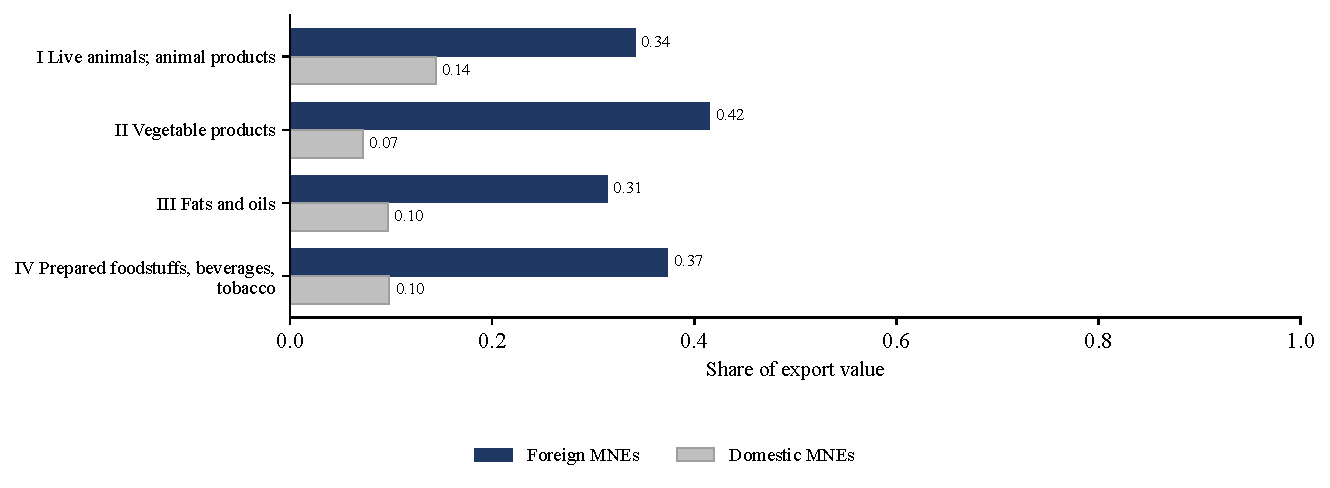
\includegraphics[width=0.9\textwidth,height=0.8\textheight,keepaspectratio]{figures/agro/fig_wp2_hs_section.pdf}%
  \caption{Agriculture: Multinational Share of Export Value, by HS Section}%
  \label{fig:sc_hs_section_f_agro}%
  \par\vspace{2pt}%
  \parbox{0.92\textwidth}{\footnotesize %
  \textit{Notes:} Shares of agricultural export value (HS 01--24), all available years pooled. HS sections.\\[3pt]%
  \textit{Source:} Authors' calculations based on customs data matched to Orbis and Dun \& Bradstreet.}%
  \end{figure}
% ---- Figure: Agriculture: Foreign-Multinational Share of Export Value, by Exporting Country and HS Section
\begin{figure}[H]\centering%
  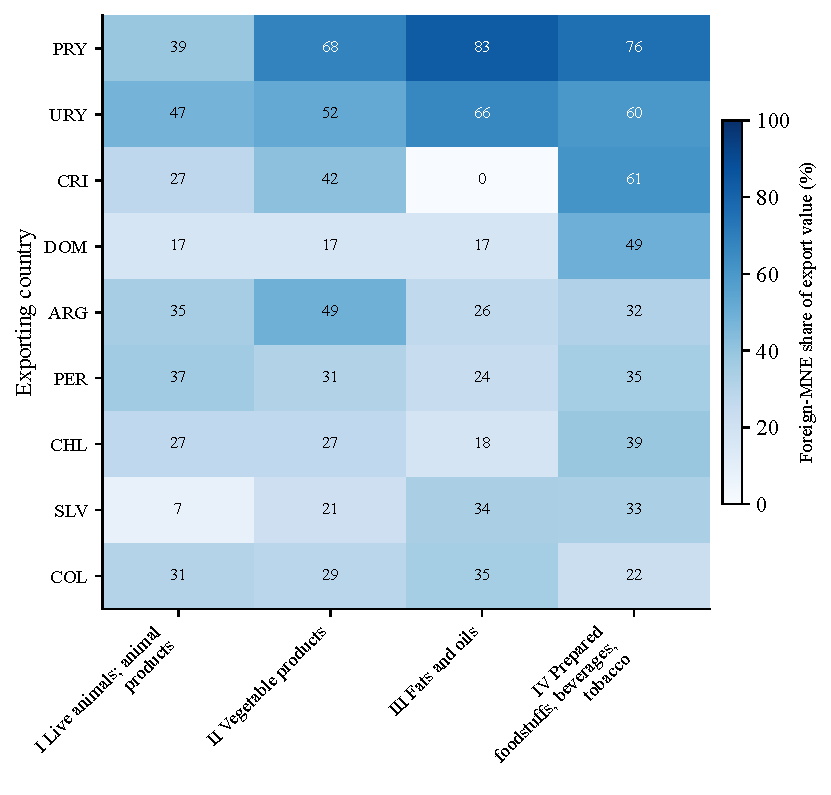
\includegraphics[width=0.95\textwidth,height=0.8\textheight,keepaspectratio]{figures/agro/fig_wp2_origin_x_hs_section.pdf}%
  \caption{Agriculture: Foreign-Multinational Share of Export Value, by Exporting Country and HS Section}%
  \label{fig:sc_hs_section_hm_agro}%
  \par\vspace{2pt}%
  \parbox{0.92\textwidth}{\footnotesize %
  \textit{Notes:} Percent of each group's export value in each country shipped by foreign MNEs. HS sections.\\[3pt]%
  \textit{Source:} Authors' calculations based on customs data matched to Orbis and Dun \& Bradstreet.}%
  \end{figure}
% ---- Table: Agriculture: Exports by Exporting Country and HS Section
\begin{table}[H]\centering\footnotesize%
  \caption{Agriculture: Exports by Exporting Country and HS Section}%
  \label{tab:sc_hs_section_ht_agro}%
  \adjustbox{max width=\textwidth, max totalheight=0.8\textheight}{\begin{tabular}{lrrrrr}
\toprule
Origin & I Live animals; animal products & II Vegetable products & III Fats and oils & IV Prepared foodstuffs, beverages, tobacco & All \\
\midrule
\multicolumn{6}{l}{\textit{Panel A: composition of the origin's exports, \% (rows sum to 100)}} \\
ARG & 13.1 & 36.4 & 13.2 & 37.3 & 100.0 \\
CHL & 36.9 & 36.5 & 1.3 & 25.4 & 100.0 \\
COL & 5.3 & 69.1 & 6.0 & 19.6 & 100.0 \\
CRI & 7.4 & 59.3 & 4.3 & 29.0 & 100.0 \\
DOM & 1.9 & 23.2 & 1.5 & 73.4 & 100.0 \\
PER & 11.3 & 45.5 & 5.1 & 38.1 & 100.0 \\
PRY & 19.6 & 51.8 & 9.4 & 19.2 & 100.0 \\
SLV & 4.6 & 27.2 & 1.9 & 66.3 & 100.0 \\
URY & 42.3 & 38.7 & 2.8 & 16.2 & 100.0 \\
All origins & 16.6 & 42.9 & 8.2 & 32.2 & 100.0 \\
\midrule
\multicolumn{6}{l}{\textit{Panel B: foreign-MNE share of export value, \%}} \\
ARG & 34.8 & 49.0 & 26.4 & 31.9 & 37.8 \\
CHL & 26.6 & 26.8 & 17.7 & 38.8 & 29.6 \\
COL & 30.7 & 28.7 & 35.4 & 22.2 & 28.0 \\
CRI & 27.4 & 41.6 & 0.3 & 61.5 & 44.5 \\
DOM & 16.8 & 17.0 & 16.7 & 49.3 & 40.7 \\
PER & 36.7 & 31.0 & 23.7 & 35.5 & 33.0 \\
PRY & 38.9 & 67.6 & 83.1 & 75.7 & 65.0 \\
SLV & 7.4 & 21.1 & 33.9 & 33.5 & 28.9 \\
URY & 47.4 & 52.2 & 66.4 & 60.1 & 51.8 \\
All origins & 34.1 & 41.5 & 31.4 & 37.4 & 38.1 \\
\bottomrule
\end{tabular}
}%
  \par\vspace{3pt}%
  \begin{minipage}{0.95\textwidth}\footnotesize %
  \textit{Notes:} Panel A: composition of each country's exports in the sector (rows add to 100). Panel B: percent of each cell's export value shipped by foreign MNEs. HS sections.\\[3pt]%
  \textit{Source:} Authors' calculations based on customs data matched to Orbis and Dun \& Bradstreet.%
  \end{minipage}%
  \end{table}
% ---- Table: Agriculture: Exports by HS Section and Parent Country
\begin{table}[H]\centering\footnotesize%
  \caption{Agriculture: Exports by HS Section and Parent Country}%
  \label{tab:sc_hs_section_par_agro}%
  \adjustbox{max width=\textwidth, max totalheight=0.8\textheight}{\begin{tabular}{lrrrrrrrrrrrr}
\toprule
HS section & USA & CHE & NLD & LIE & BRA & ESP & DEU & SAU & LUX & GBR & Other & Domestic \\
\midrule
I Live animals; animal products & 1.0 & 0.7 & 0.8 & 0.1 & 2.9 & 2.9 & 0.0 & 5.5 & 1.1 & 0.9 & 18.2 & 14.4 \\
II Vegetable products & 11.8 & 2.5 & 4.0 & 2.7 & 1.2 & 1.0 & 2.3 & 0.0 & 1.3 & 0.5 & 14.2 & 7.3 \\
III Fats and oils & 5.4 & 7.4 & 6.0 & 3.5 & 0.3 & 0.1 & 0.0 & 0.1 & 0.1 & 0.9 & 7.6 & 9.7 \\
IV Prepared foodstuffs, beverages, tobacco & 7.2 & 5.8 & 2.6 & 3.4 & 0.8 & 1.1 & 0.6 & 0.5 & 0.7 & 1.4 & 13.4 & 9.8 \\
\bottomrule
\end{tabular}
}%
  \par\vspace{3pt}%
  \begin{minipage}{0.95\textwidth}\footnotesize %
  \textit{Notes:} Percent of each group's export value, by country of the ultimate parent of foreign MNEs; domestic MNEs shown for comparison. HS sections.\\[3pt]%
  \textit{Source:} Authors' calculations based on customs data matched to Orbis and Dun \& Bradstreet.%
  \end{minipage}%
  \end{table}

\subsection{By End Use}
% ---- Table: Agriculture: Exports and Multinational Shares, by End Use
\begin{table}[H]\centering\footnotesize%
  \caption{Agriculture: Exports and Multinational Shares, by End Use}%
  \label{tab:sc_bec_enduse_agro}%
  \adjustbox{max width=\textwidth, max totalheight=0.8\textheight}{\begin{tabular}{@{}l r r r r l@{}}
\toprule
BEC end use & Total exports (US\$bn/yr) & MNE exports (US\$bn/yr) & Foreign (\%) & Domestic (\%) & Leading parents (share of foreign) \\
\midrule
Intermediate & 42.5 & 21.4 & 41.1 & 9.0 & USA 0.30, CHE 0.16, NLD 0.13 \\
Consumption & 30.4 & 13.7 & 35.1 & 9.9 & USA 0.16, ESP 0.09, SAU 0.08 \\
Capital & 0.0 & 0.0 & 16.8 & 2.0 & GBR 0.35, SAU 0.33, NLD 0.28 \\
\midrule
All & 72.9 & 35.0 & 38.5 & 9.4 & \\
\bottomrule
\end{tabular}
}%
  \par\vspace{3pt}%
  \begin{minipage}{0.95\textwidth}\footnotesize %
  \textit{Notes:} End use from BEC Rev.\,4. Foreign and domestic: percent of the group's export value. Leading parents: the three largest parent countries and their share of the row's foreign-MNE exports. Values are annual averages in US\$ billion.\\[3pt]%
  \textit{Source:} Authors' calculations based on customs data matched to Orbis and Dun \& Bradstreet.%
  \end{minipage}%
  \end{table}
% ---- Figure: Agriculture: Multinational Share of Export Value, by End Use
\begin{figure}[H]\centering%
  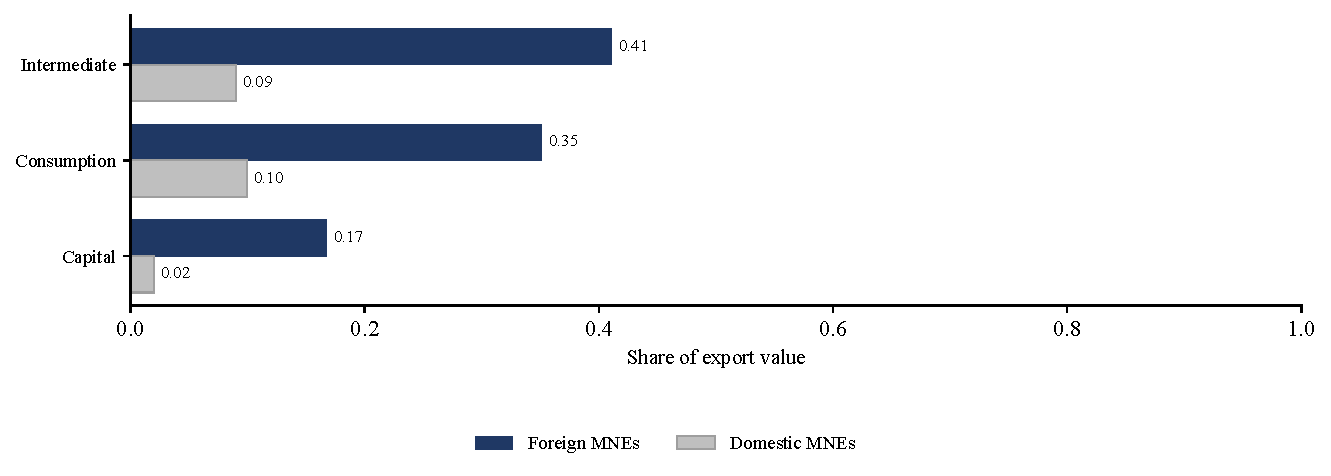
\includegraphics[width=0.9\textwidth,height=0.8\textheight,keepaspectratio]{figures/agro/fig_wp2_bec_enduse.pdf}%
  \caption{Agriculture: Multinational Share of Export Value, by End Use}%
  \label{fig:sc_bec_enduse_f_agro}%
  \par\vspace{2pt}%
  \parbox{0.92\textwidth}{\footnotesize %
  \textit{Notes:} Shares of agricultural export value (HS 01--24), all available years pooled. End use from BEC Rev.\,4.\\[3pt]%
  \textit{Source:} Authors' calculations based on customs data matched to Orbis and Dun \& Bradstreet.}%
  \end{figure}
% ---- Figure: Agriculture: Foreign-Multinational Share of Export Value, by Exporting Country and End Use
\begin{figure}[H]\centering%
  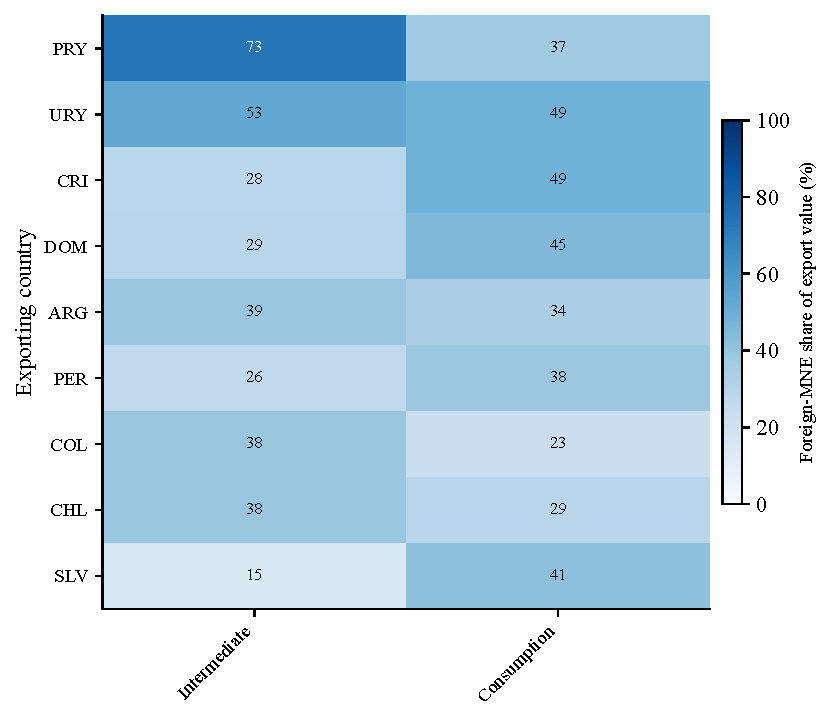
\includegraphics[width=0.95\textwidth,height=0.8\textheight,keepaspectratio]{figures/agro/fig_wp2_origin_x_bec_enduse.pdf}%
  \caption{Agriculture: Foreign-Multinational Share of Export Value, by Exporting Country and End Use}%
  \label{fig:sc_bec_enduse_hm_agro}%
  \par\vspace{2pt}%
  \parbox{0.92\textwidth}{\footnotesize %
  \textit{Notes:} Percent of each group's export value in each country shipped by foreign MNEs. End use from BEC Rev.\,4.\\[3pt]%
  \textit{Source:} Authors' calculations based on customs data matched to Orbis and Dun \& Bradstreet.}%
  \end{figure}
% ---- Table: Agriculture: Exports by Exporting Country and End Use
\begin{table}[H]\centering\footnotesize%
  \caption{Agriculture: Exports by Exporting Country and End Use}%
  \label{tab:sc_bec_enduse_ht_agro}%
  \adjustbox{max width=\textwidth, max totalheight=0.8\textheight}{\begin{tabular}{lrrrr}
\toprule
Origin & Intermediate & Consumption & Capital & All \\
\midrule
\multicolumn{5}{l}{\textit{Panel A: composition of the origin's exports, \% (rows sum to 100)}} \\
ARG & 73.1 & 26.9 & 0.0 & 100.0 \\
CHL & 12.6 & 87.3 & 0.0 & 100.0 \\
COL & 49.6 & 50.4 & 0.0 & 100.0 \\
CRI & 20.9 & 79.0 & 0.0 & 100.0 \\
DOM & 27.9 & 72.1 & 0.0 & 100.0 \\
PER & 44.1 & 55.9 & 0.0 & 100.0 \\
PRY & 78.3 & 21.7 & 0.0 & 100.0 \\
SLV & 44.2 & 55.8 & 0.0 & 100.0 \\
URY & 40.1 & 59.8 & 0.2 & 100.0 \\
All origins & 56.0 & 44.0 & 0.0 & 100.0 \\
\midrule
\multicolumn{5}{l}{\textit{Panel B: foreign-MNE share of export value, \%}} \\
ARG & 38.5 & 33.7 & 5.4 & 37.2 \\
CHL & 38.4 & 29.1 & 95.3 & 30.3 \\
COL & 38.4 & 22.5 & 4.4 & 30.4 \\
CRI & 28.0 & 48.7 & 85.6 & 44.4 \\
DOM & 29.3 & 45.0 & 0.1 & 40.7 \\
PER & 26.2 & 38.3 & 4.9 & 33.0 \\
PRY & 72.9 & 36.5 & 32.6 & 65.0 \\
SLV & 14.7 & 41.5 & 5.4 & 29.6 \\
URY & 52.7 & 48.6 & 16.4 & 50.2 \\
All origins & 41.1 & 35.1 & 16.8 & 38.5 \\
\bottomrule
\end{tabular}
}%
  \par\vspace{3pt}%
  \begin{minipage}{0.95\textwidth}\footnotesize %
  \textit{Notes:} Panel A: composition of each country's exports in the sector (rows add to 100). Panel B: percent of each cell's export value shipped by foreign MNEs. End use from BEC Rev.\,4.\\[3pt]%
  \textit{Source:} Authors' calculations based on customs data matched to Orbis and Dun \& Bradstreet.%
  \end{minipage}%
  \end{table}
% ---- Table: Agriculture: Exports by End Use and Parent Country
\begin{table}[H]\centering\footnotesize%
  \caption{Agriculture: Exports by End Use and Parent Country}%
  \label{tab:sc_bec_enduse_par_agro}%
  \adjustbox{max width=\textwidth, max totalheight=0.8\textheight}{\begin{tabular}{lrrrrrrrrrrrr}
\toprule
BEC end use & USA & CHE & NLD & LIE & BRA & ESP & DEU & SAU & LUX & GBR & Other & Domestic \\
\midrule
Intermediate & 11.3 & 6.0 & 5.0 & 4.8 & 1.2 & 0.2 & 1.9 & 0.1 & 0.9 & 0.7 & 9.0 & 9.0 \\
Consumption & 4.4 & 1.4 & 0.9 & 0.1 & 1.2 & 2.6 & 0.5 & 2.2 & 1.2 & 1.2 & 19.5 & 9.9 \\
Capital & 0.2 & 0.0 & 3.8 & 0.0 & 0.0 & 0.0 & 0.0 & 4.5 & 0.0 & 4.9 & 3.4 & 2.0 \\
\bottomrule
\end{tabular}
}%
  \par\vspace{3pt}%
  \begin{minipage}{0.95\textwidth}\footnotesize %
  \textit{Notes:} Percent of each group's export value, by country of the ultimate parent of foreign MNEs; domestic MNEs shown for comparison. End use from BEC Rev.\,4.\\[3pt]%
  \textit{Source:} Authors' calculations based on customs data matched to Orbis and Dun \& Bradstreet.%
  \end{minipage}%
  \end{table}

\subsection{By BEC Category}
% ---- Table: Agriculture: Exports and Multinational Shares, by BEC Category
\begin{table}[H]\centering\footnotesize%
  \caption{Agriculture: Exports and Multinational Shares, by BEC Category}%
  \label{tab:sc_bec4_agro}%
  \adjustbox{max width=\textwidth, max totalheight=0.8\textheight}{\begin{tabular}{@{}l r r r r l@{}}
\toprule
BEC Rev.\,4 category & Total exports (US\$bn/yr) & MNE exports (US\$bn/yr) & Foreign (\%) & Domestic (\%) & Leading parents (share of foreign) \\
\midrule
122 Food \& bev., processed, for households & 17.7 & 8.6 & 37.0 & 12.1 & USA 0.16, SAU 0.12, BRA 0.07 \\
111 Food \& bev., primary, for industry & 14.0 & 7.9 & 48.9 & 7.4 & USA 0.40, NLD 0.11, DEU 0.10 \\
22 Industrial supplies, processed & 13.8 & 6.4 & 34.9 & 11.2 & CHE 0.28, LIE 0.19, USA 0.17 \\
112 Food \& bev., primary, for households & 10.3 & 4.0 & 31.9 & 6.6 & ESP 0.22, USA 0.13, JOR 0.09 \\
121 Food \& bev., processed, for industry & 8.4 & 3.5 & 30.9 & 10.5 & CHE 0.20, USA 0.18, NLD 0.16 \\
21 Industrial supplies, primary & 6.3 & 3.6 & 50.4 & 6.0 & USA 0.37, NLD 0.15, CHE 0.14 \\
63 Consumer goods, non-durable & 2.4 & 1.1 & 35.2 & 7.9 & USA 0.25, HKG 0.17, GBR 0.09 \\
41 Capital goods & 0.0 & 0.0 & 16.8 & 2.0 & GBR 0.35, SAU 0.33, NLD 0.28 \\
\midrule
All & 72.9 & 35.0 & 38.5 & 9.4 & \\
\bottomrule
\end{tabular}
}%
  \par\vspace{3pt}%
  \begin{minipage}{0.95\textwidth}\footnotesize %
  \textit{Notes:} Categories of BEC Rev.\,4. Foreign and domestic: percent of the group's export value. Leading parents: the three largest parent countries and their share of the row's foreign-MNE exports. Values are annual averages in US\$ billion.\\[3pt]%
  \textit{Source:} Authors' calculations based on customs data matched to Orbis and Dun \& Bradstreet.%
  \end{minipage}%
  \end{table}
% ---- Figure: Agriculture: Multinational Share of Export Value, by BEC Category
\begin{figure}[H]\centering%
  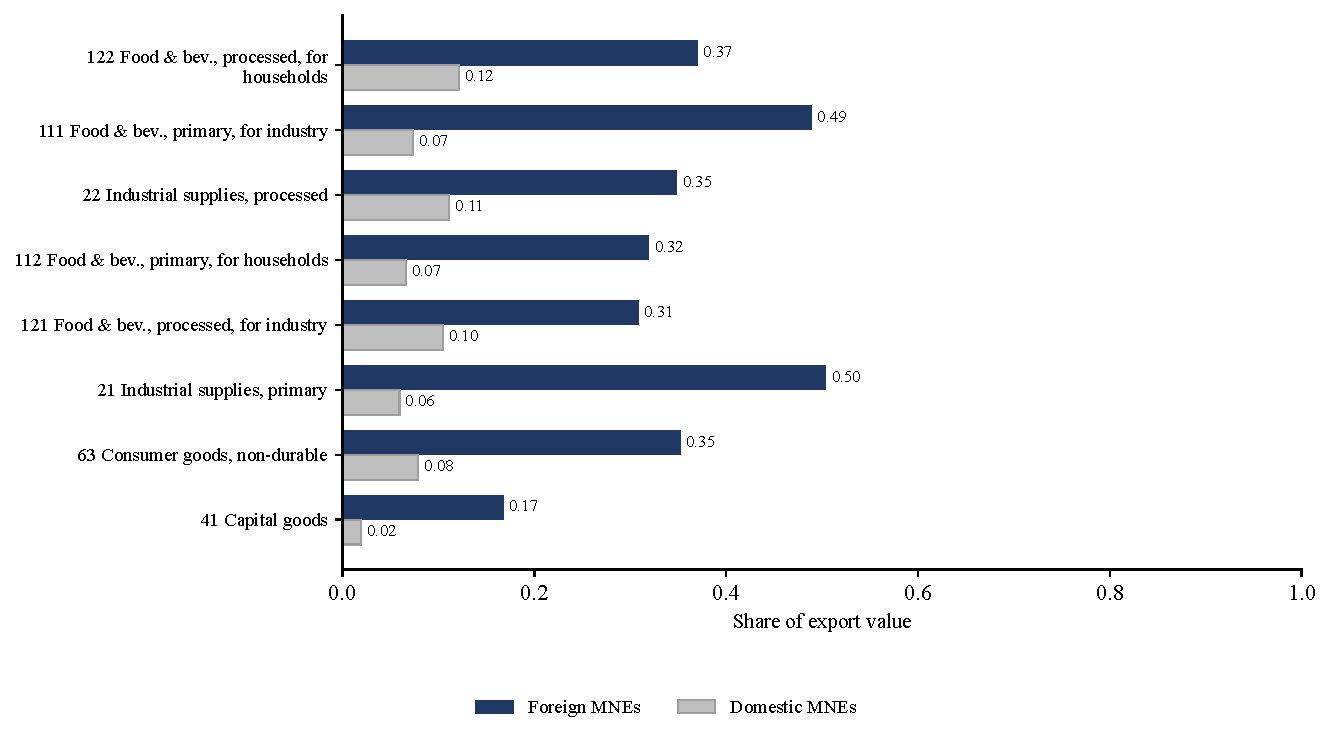
\includegraphics[width=0.9\textwidth,height=0.8\textheight,keepaspectratio]{figures/agro/fig_wp2_bec4.pdf}%
  \caption{Agriculture: Multinational Share of Export Value, by BEC Category}%
  \label{fig:sc_bec4_f_agro}%
  \par\vspace{2pt}%
  \parbox{0.92\textwidth}{\footnotesize %
  \textit{Notes:} Shares of agricultural export value (HS 01--24), all available years pooled. Categories of BEC Rev.\,4.\\[3pt]%
  \textit{Source:} Authors' calculations based on customs data matched to Orbis and Dun \& Bradstreet.}%
  \end{figure}
% ---- Figure: Agriculture: Foreign-Multinational Share of Export Value, by Exporting Country and BEC Category
\begin{figure}[H]\centering%
  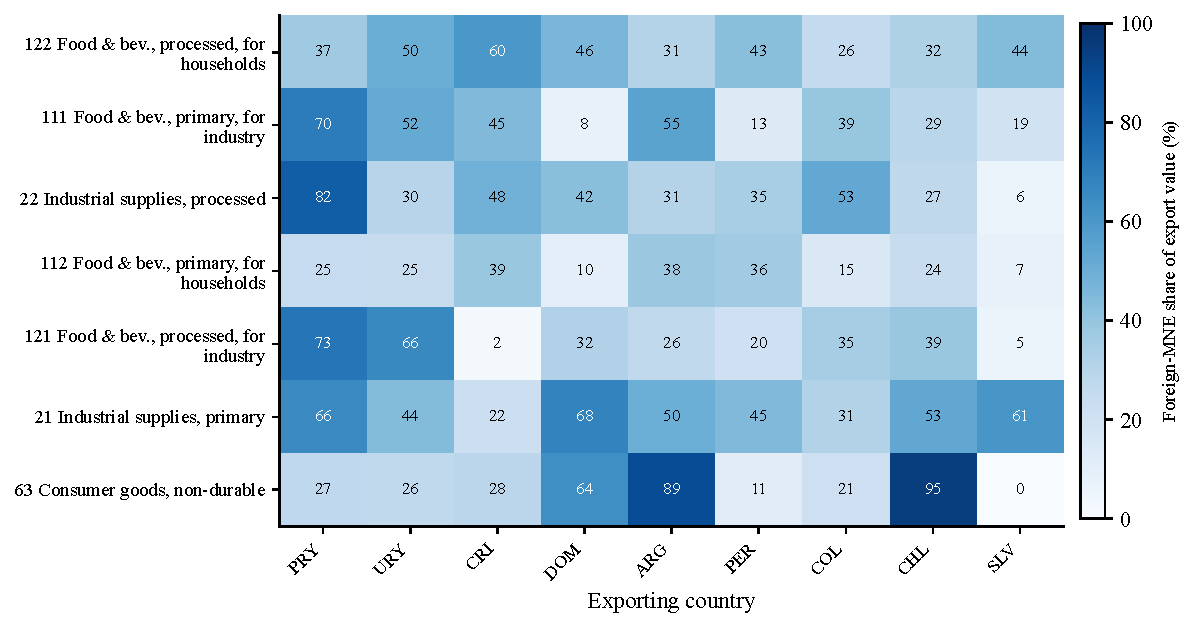
\includegraphics[width=0.95\textwidth,height=0.8\textheight,keepaspectratio]{figures/agro/fig_wp2_origin_x_bec4.pdf}%
  \caption{Agriculture: Foreign-Multinational Share of Export Value, by Exporting Country and BEC Category}%
  \label{fig:sc_bec4_hm_agro}%
  \par\vspace{2pt}%
  \parbox{0.92\textwidth}{\footnotesize %
  \textit{Notes:} Percent of each group's export value in each country shipped by foreign MNEs. Categories of BEC Rev.\,4.\\[3pt]%
  \textit{Source:} Authors' calculations based on customs data matched to Orbis and Dun \& Bradstreet.}%
  \end{figure}
% ---- Table: Agriculture: Exports by Exporting Country and BEC Category
\begin{table}[H]\centering\footnotesize%
  \caption{Agriculture: Exports by Exporting Country and BEC Category}%
  \label{tab:sc_bec4_ht_agro}%
  \adjustbox{max width=\textwidth, max totalheight=0.8\textheight}{\begin{tabular}{lrrrrrrrrrr}
\toprule
Sub-sector & ARG & CHL & COL & CRI & DOM & PER & PRY & SLV & URY & All \\
\midrule
\multicolumn{11}{l}{\textit{Panel A: composition of the origin's exports, \% (columns sum to 100)}} \\
122 Food \& bev., processed, for households & 18.5 & 46.2 & 22.5 & 37.7 & 21.2 & 18.2 & 20.8 & 51.8 & 55.8 & 25.4 \\
111 Food \& bev., primary, for industry & 16.1 & 0.5 & 39.2 & 9.7 & 11.1 & 13.7 & 42.0 & 22.2 & 28.2 & 19.0 \\
22 Industrial supplies, processed & 28.2 & 5.4 & 0.6 & 1.4 & 2.0 & 21.5 & 17.3 & 6.9 & 2.2 & 17.9 \\
112 Food \& bev., primary, for households & 8.0 & 40.3 & 5.2 & 39.8 & 18.0 & 37.6 & 0.3 & 3.4 & 3.2 & 15.1 \\
121 Food \& bev., processed, for industry & 15.3 & 2.3 & 8.1 & 6.6 & 9.9 & 6.8 & 10.7 & 13.3 & 7.5 & 11.0 \\
21 Industrial supplies, primary & 13.4 & 4.4 & 1.6 & 3.2 & 4.9 & 2.1 & 8.3 & 1.9 & 2.2 & 8.2 \\
63 Consumer goods, non-durable & 0.4 & 0.8 & 22.8 & 1.6 & 33.0 & 0.2 & 0.6 & 0.5 & 0.8 & 3.5 \\
41 Capital goods & 0.0 & 0.0 & 0.0 & 0.0 & 0.0 & 0.0 & 0.0 & 0.0 & 0.2 & 0.0 \\
All sub-sectors & 100.0 & 100.0 & 100.0 & 100.0 & 100.0 & 100.0 & 100.0 & 100.0 & 100.0 & 100.0 \\
\midrule
\multicolumn{11}{l}{\textit{Panel B: foreign-MNE share of export value, \%}} \\
122 Food \& bev., processed, for households & 30.8 & 32.3 & 25.6 & 60.1 & 46.2 & 42.6 & 37.0 & 44.1 & 50.3 & 37.0 \\
111 Food \& bev., primary, for industry & 54.8 & 28.7 & 39.2 & 44.7 & 7.7 & 12.9 & 70.4 & 19.1 & 51.7 & 48.9 \\
22 Industrial supplies, processed & 30.5 & 27.1 & 52.6 & 48.1 & 42.4 & 34.7 & 82.1 & 6.0 & 29.5 & 34.9 \\
112 Food \& bev., primary, for households & 37.9 & 24.0 & 14.7 & 38.8 & 9.7 & 36.3 & 24.6 & 7.1 & 24.5 & 31.9 \\
121 Food \& bev., processed, for industry & 26.3 & 38.9 & 35.0 & 2.2 & 31.8 & 20.5 & 73.4 & 5.3 & 65.7 & 30.9 \\
21 Industrial supplies, primary & 49.8 & 53.0 & 31.0 & 21.6 & 67.6 & 44.8 & 65.6 & 60.5 & 44.0 & 50.4 \\
63 Consumer goods, non-durable & 88.8 & 94.6 & 21.2 & 28.3 & 63.6 & 11.2 & 26.8 & 0.2 & 26.4 & 35.2 \\
41 Capital goods & 5.4 & 95.3 & 4.4 & 85.6 & 0.1 & 4.9 & 32.6 & 5.4 & 16.4 & 16.8 \\
All sub-sectors & 37.2 & 30.3 & 30.4 & 44.4 & 40.7 & 33.0 & 65.0 & 29.6 & 50.2 & 38.5 \\
\bottomrule
\end{tabular}
}%
  \par\vspace{3pt}%
  \begin{minipage}{0.95\textwidth}\footnotesize %
  \textit{Notes:} Panel A: composition of each country's exports in the sector (rows add to 100). Panel B: percent of each cell's export value shipped by foreign MNEs. Categories of BEC Rev.\,4.\\[3pt]%
  \textit{Source:} Authors' calculations based on customs data matched to Orbis and Dun \& Bradstreet.%
  \end{minipage}%
  \end{table}
% ---- Table: Agriculture: Exports by BEC Category and Parent Country
\begin{table}[H]\centering\footnotesize%
  \caption{Agriculture: Exports by BEC Category and Parent Country}%
  \label{tab:sc_bec4_par_agro}%
  \adjustbox{max width=\textwidth, max totalheight=0.8\textheight}{\begin{tabular}{lrrrrrrrrrrrr}
\toprule
BEC Rev.\,4 category & USA & CHE & NLD & LIE & BRA & ESP & DEU & SAU & LUX & GBR & Other & Domestic \\
\midrule
122 Food \& bev., processed, for households & 4.9 & 2.1 & 1.2 & 0.2 & 2.1 & 1.3 & 0.5 & 3.8 & 1.1 & 1.4 & 18.3 & 12.1 \\
111 Food \& bev., primary, for industry & 17.7 & 3.0 & 5.1 & 3.9 & 2.2 & 0.1 & 4.3 & 0.0 & 0.5 & 0.2 & 11.8 & 7.4 \\
22 Industrial supplies, processed & 5.7 & 9.2 & 4.5 & 6.5 & 0.3 & 0.5 & 0.2 & 0.1 & 0.0 & 1.2 & 6.5 & 11.2 \\
112 Food \& bev., primary, for households & 3.1 & 0.2 & 0.4 & 0.0 & 0.0 & 5.2 & 0.5 & 0.1 & 1.6 & 0.4 & 20.5 & 6.6 \\
121 Food \& bev., processed, for industry & 4.9 & 5.5 & 4.5 & 3.3 & 0.3 & 0.0 & 0.2 & 0.0 & 3.4 & 1.1 & 7.6 & 10.5 \\
21 Industrial supplies, primary & 17.3 & 6.4 & 6.7 & 5.1 & 1.7 & 0.2 & 2.5 & 0.5 & 0.1 & 0.3 & 9.7 & 6.0 \\
63 Consumer goods, non-durable & 7.1 & 1.9 & 0.0 & 0.0 & 0.1 & 0.2 & 0.0 & 0.0 & 0.0 & 2.7 & 23.1 & 7.9 \\
41 Capital goods & 0.2 & 0.0 & 3.8 & 0.0 & 0.0 & 0.0 & 0.0 & 4.5 & 0.0 & 4.9 & 3.4 & 2.0 \\
\bottomrule
\end{tabular}
}%
  \par\vspace{3pt}%
  \begin{minipage}{0.95\textwidth}\footnotesize %
  \textit{Notes:} Percent of each group's export value, by country of the ultimate parent of foreign MNEs; domestic MNEs shown for comparison. Categories of BEC Rev.\,4.\\[3pt]%
  \textit{Source:} Authors' calculations based on customs data matched to Orbis and Dun \& Bradstreet.%
  \end{minipage}%
  \end{table}

\subsection{By SITC Division}
% ---- Table: Agriculture: Exports and Multinational Shares, by SITC Division
\begin{table}[H]\centering\footnotesize%
  \caption{Agriculture: Exports and Multinational Shares, by SITC Division}%
  \label{tab:sc_sitc2_agro}%
  \adjustbox{max width=\textwidth, max totalheight=0.8\textheight}{\begin{tabular}{@{}l r r r r l@{}}
\toprule
SITC Rev.\,3 division & Total exports (US\$bn/yr) & MNE exports (US\$bn/yr) & Foreign (\%) & Domestic (\%) & Leading parents (share of foreign) \\
\midrule
08 Animal feed & 13.8 & 6.6 & 35.7 & 11.5 & CHE 0.28, LIE 0.19, USA 0.18 \\
05 Vegetables \& fruit & 10.6 & 4.0 & 32.6 & 5.8 & ESP 0.14, USA 0.13, PAN 0.11 \\
04 Cereals & 10.3 & 5.9 & 48.6 & 8.2 & USA 0.33, CHE 0.14, NLD 0.14 \\
22 Oil seeds & 6.7 & 4.4 & 61.6 & 4.1 & USA 0.54, NLD 0.14, LIE 0.08 \\
07 Coffee, tea, cocoa, spices & 5.1 & 2.3 & 30.4 & 15.6 & DEU 0.41, ITA 0.14, SGP 0.12 \\
42 Fixed vegetable oils & 6.0 & 2.5 & 30.8 & 10.2 & CHE 0.27, NLD 0.24, USA 0.23 \\
01 Meat & 5.2 & 2.4 & 34.8 & 13.1 & SAU 0.46, BRA 0.26, JPN 0.08 \\
03 Fish \& seafood & 3.4 & 1.8 & 41.9 & 9.5 & ESP 0.32, LUX 0.11, ITA 0.10 \\
29 Crude animal/veg. materials & 2.2 & 0.8 & 27.3 & 9.0 & DEU 0.10, ARG 0.09, BGR 0.08 \\
11 Beverages & 2.2 & 0.8 & 28.6 & 9.2 & LUX 0.17, PAN 0.15, GBR 0.12 \\
02 Dairy \& eggs & 1.9 & 1.0 & 28.0 & 20.3 & NLD 0.20, CHE 0.19, ROU 0.19 \\
09 Misc. edible products & 1.7 & 1.2 & 70.9 & 2.3 & USA 0.46, CHE 0.17, FRA 0.09 \\
06 Sugar \& honey & 1.4 & 0.5 & 19.3 & 14.7 & USA 0.50, KOR 0.18, LIE 0.10 \\
12 Tobacco & 1.2 & 0.7 & 54.8 & 0.2 & USA 0.36, HKG 0.25, GBR 0.12 \\
41 Animal oils \& fats & 0.5 & 0.2 & 23.0 & 11.0 & BMU 0.31, PAN 0.23, GBR 0.16 \\
Other & 0.6 & 0.1 & 21.6 & 1.9 & CHE 0.21, USA 0.20, ROU 0.10 \\
\midrule
All & 72.9 & 35.0 & 38.5 & 9.4 & \\
\bottomrule
\end{tabular}
}%
  \par\vspace{3pt}%
  \begin{minipage}{0.95\textwidth}\footnotesize %
  \textit{Notes:} SITC Rev.\,3 divisions; HS6 products without an SITC correspondence are excluded. Foreign and domestic: percent of the group's export value. Leading parents: the three largest parent countries and their share of the row's foreign-MNE exports. Values are annual averages in US\$ billion.\\[3pt]%
  \textit{Source:} Authors' calculations based on customs data matched to Orbis and Dun \& Bradstreet.%
  \end{minipage}%
  \end{table}
% ---- Figure: Agriculture: Multinational Share of Export Value, by SITC Division
\begin{figure}[H]\centering%
  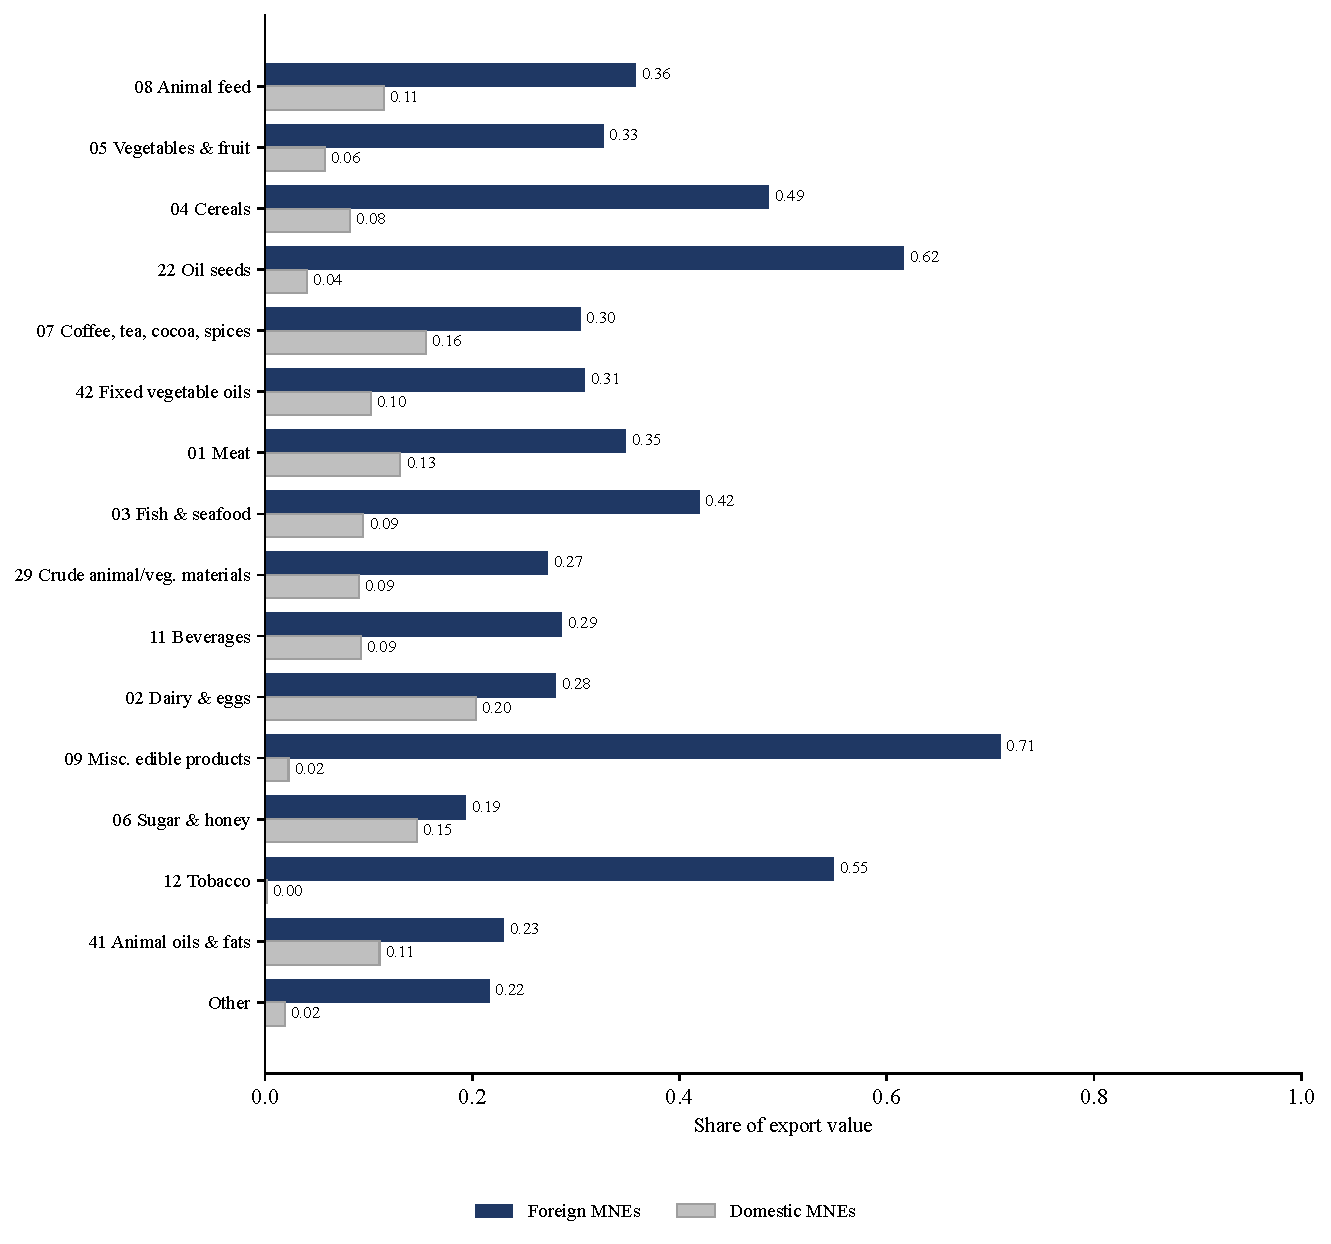
\includegraphics[width=0.9\textwidth,height=0.8\textheight,keepaspectratio]{figures/agro/fig_wp2_sitc2.pdf}%
  \caption{Agriculture: Multinational Share of Export Value, by SITC Division}%
  \label{fig:sc_sitc2_f_agro}%
  \par\vspace{2pt}%
  \parbox{0.92\textwidth}{\footnotesize %
  \textit{Notes:} Shares of agricultural export value (HS 01--24), all available years pooled. SITC Rev.\,3 divisions; HS6 products without an SITC correspondence are excluded.\\[3pt]%
  \textit{Source:} Authors' calculations based on customs data matched to Orbis and Dun \& Bradstreet.}%
  \end{figure}
% ---- Figure: Agriculture: Foreign-Multinational Share of Export Value, by Exporting Country and SITC Division
\begin{figure}[H]\centering%
  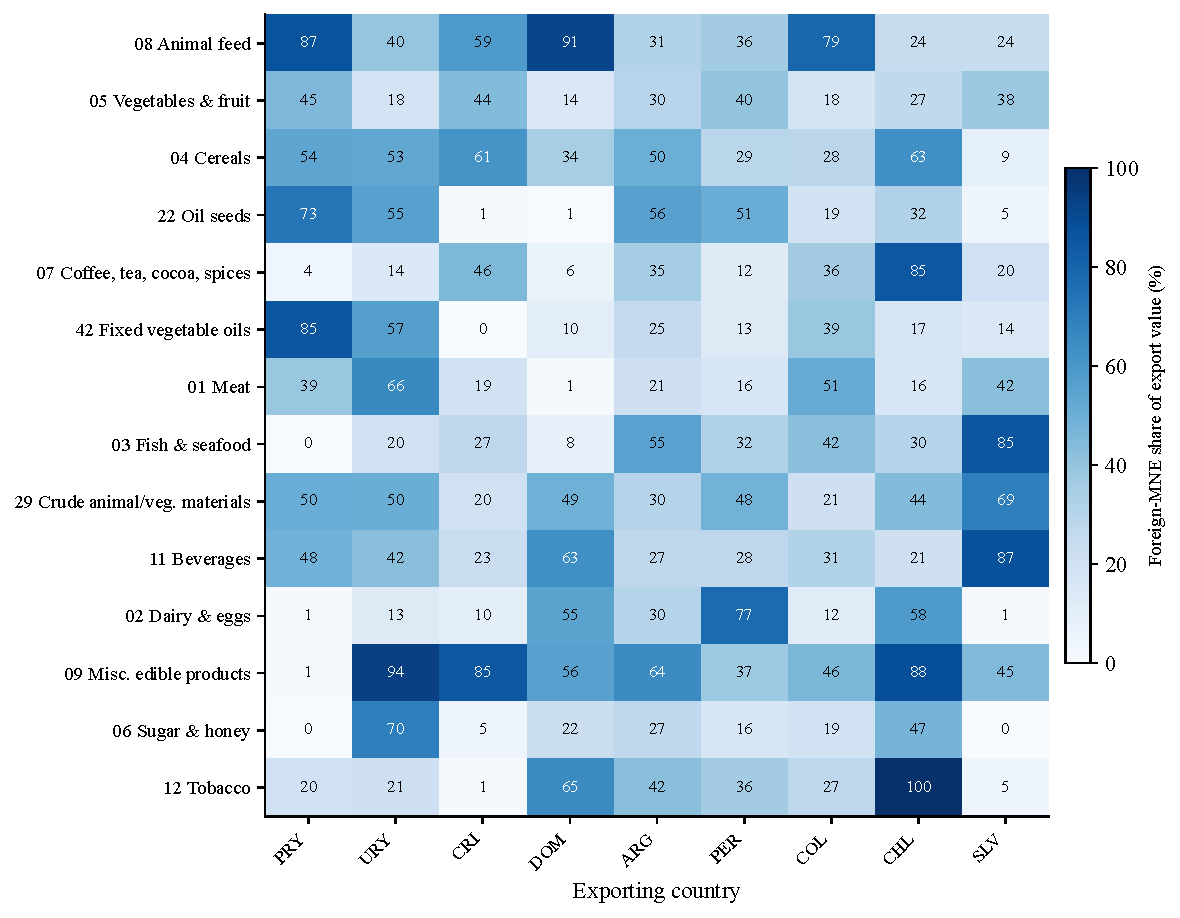
\includegraphics[width=0.95\textwidth,height=0.8\textheight,keepaspectratio]{figures/agro/fig_wp2_origin_x_sitc2.pdf}%
  \caption{Agriculture: Foreign-Multinational Share of Export Value, by Exporting Country and SITC Division}%
  \label{fig:sc_sitc2_hm_agro}%
  \par\vspace{2pt}%
  \parbox{0.92\textwidth}{\footnotesize %
  \textit{Notes:} Percent of each group's export value in each country shipped by foreign MNEs. SITC Rev.\,3 divisions; HS6 products without an SITC correspondence are excluded.\\[3pt]%
  \textit{Source:} Authors' calculations based on customs data matched to Orbis and Dun \& Bradstreet.}%
  \end{figure}
% ---- Table: Agriculture: Exports by Exporting Country and SITC Division
\begin{table}[H]\centering\footnotesize%
  \caption{Agriculture: Exports by Exporting Country and SITC Division}%
  \label{tab:sc_sitc2_ht_agro}%
  \adjustbox{max width=\textwidth, max totalheight=0.8\textheight}{\begin{tabular}{lrrrrrrrrrr}
\toprule
Sub-sector & ARG & CHL & COL & CRI & DOM & PER & PRY & SLV & URY & All \\
\midrule
\multicolumn{11}{l}{\textit{Panel A: composition of the origin's exports, \% (columns sum to 100)}} \\
08 Animal feed & 29.1 & 4.4 & 0.6 & 1.5 & 0.7 & 20.5 & 16.5 & 1.7 & 1.0 & 17.8 \\
05 Vegetables \& fruit & 7.6 & 43.7 & 5.9 & 48.1 & 20.8 & 36.4 & 0.3 & 7.2 & 2.0 & 15.6 \\
04 Cereals & 20.9 & 2.8 & 2.5 & 3.6 & 5.6 & 3.3 & 12.5 & 19.6 & 20.5 & 13.4 \\
22 Oil seeds & 9.5 & 0.4 & 0.0 & 0.1 & 0.0 & 0.3 & 38.6 & 0.1 & 20.6 & 8.6 \\
07 Coffee, tea, cocoa, spices & 0.9 & 0.7 & 45.4 & 9.9 & 11.1 & 14.5 & 0.1 & 21.8 & 0.3 & 7.9 \\
42 Fixed vegetable oils & 12.8 & 0.5 & 6.2 & 5.2 & 1.2 & 0.5 & 9.1 & 0.2 & 0.1 & 7.7 \\
01 Meat & 5.9 & 9.2 & 1.4 & 2.8 & 0.7 & 0.1 & 18.3 & 1.3 & 30.2 & 7.0 \\
03 Fish \& seafood & 3.9 & 10.4 & 1.6 & 1.8 & 0.6 & 13.1 & 0.0 & 9.6 & 3.0 & 4.9 \\
29 Crude animal/veg. materials & 0.4 & 3.8 & 23.4 & 3.7 & 1.0 & 2.1 & 1.1 & 1.6 & 1.5 & 3.6 \\
11 Beverages & 2.5 & 16.4 & 0.4 & 1.7 & 6.8 & 0.5 & 0.0 & 9.2 & 0.5 & 3.4 \\
02 Dairy \& eggs & 2.8 & 1.4 & 0.3 & 3.9 & 0.6 & 1.5 & 0.2 & 2.4 & 12.7 & 2.6 \\
09 Misc. edible products & 1.3 & 3.5 & 2.2 & 15.1 & 6.4 & 0.9 & 0.2 & 5.3 & 2.4 & 2.4 \\
06 Sugar \& honey & 1.1 & 0.5 & 8.8 & 1.1 & 6.7 & 0.8 & 1.1 & 12.1 & 0.6 & 2.1 \\
12 Tobacco & 0.9 & 0.8 & 0.6 & 0.3 & 37.1 & 0.1 & 0.8 & 0.0 & 1.1 & 1.5 \\
41 Animal oils \& fats & 0.0 & 1.0 & 0.0 & 0.0 & 0.0 & 4.4 & 0.3 & 0.0 & 1.3 & 0.7 \\
Other & 0.5 & 0.5 & 0.7 & 0.9 & 0.7 & 1.1 & 0.7 & 7.7 & 2.2 & 0.9 \\
All sub-sectors & 100.0 & 100.0 & 100.0 & 100.0 & 100.0 & 100.0 & 100.0 & 100.0 & 100.0 & 100.0 \\
\midrule
\multicolumn{11}{l}{\textit{Panel B: foreign-MNE share of export value, \%}} \\
08 Animal feed & 30.9 & 24.2 & 79.1 & 58.9 & 91.5 & 35.7 & 86.6 & 24.1 & 39.6 & 35.7 \\
05 Vegetables \& fruit & 29.6 & 26.5 & 17.9 & 44.0 & 14.3 & 40.0 & 45.0 & 38.0 & 18.1 & 32.6 \\
04 Cereals & 49.9 & 63.0 & 28.2 & 61.0 & 34.2 & 28.6 & 53.7 & 8.8 & 52.8 & 48.6 \\
22 Oil seeds & 55.8 & 31.8 & 18.8 & 1.2 & 0.8 & 50.5 & 73.1 & 4.8 & 55.5 & 61.6 \\
07 Coffee, tea, cocoa, spices & 35.4 & 85.1 & 36.2 & 45.6 & 6.3 & 12.4 & 4.0 & 20.2 & 13.7 & 30.4 \\
42 Fixed vegetable oils & 25.2 & 17.1 & 38.6 & 0.0 & 10.2 & 12.8 & 85.2 & 14.4 & 56.6 & 30.8 \\
01 Meat & 20.8 & 16.3 & 50.8 & 19.3 & 1.4 & 16.3 & 38.6 & 42.4 & 66.0 & 34.8 \\
03 Fish \& seafood & 55.4 & 30.4 & 42.4 & 27.4 & 7.5 & 32.0 & 0.0 & 85.4 & 19.6 & 41.9 \\
29 Crude animal/veg. materials & 29.7 & 43.9 & 20.6 & 19.7 & 49.2 & 47.8 & 50.5 & 69.3 & 50.2 & 27.3 \\
11 Beverages & 27.3 & 20.7 & 31.0 & 22.9 & 63.0 & 27.7 & 48.3 & 87.3 & 42.4 & 28.6 \\
02 Dairy \& eggs & 29.8 & 58.4 & 11.7 & 9.6 & 54.9 & 77.3 & 0.8 & 0.8 & 13.1 & 28.0 \\
09 Misc. edible products & 64.5 & 88.2 & 45.8 & 84.6 & 55.7 & 37.1 & 1.1 & 44.7 & 93.6 & 70.9 \\
06 Sugar \& honey & 26.7 & 47.4 & 19.2 & 4.9 & 22.1 & 16.2 & 0.1 & 0.1 & 69.8 & 19.3 \\
12 Tobacco & 42.3 & 99.8 & 27.4 & 1.0 & 65.0 & 35.6 & 20.0 & 5.0 & 21.5 & 54.8 \\
41 Animal oils \& fats & 26.3 & 13.3 & 41.6 & 36.8 & 89.4 & 24.9 & 28.7 & 49.8 & 20.5 & 23.0 \\
Other & 36.1 & 45.3 & 16.5 & 26.3 & 5.1 & 7.5 & 1.6 & 0.1 & 34.5 & 21.6 \\
All sub-sectors & 37.2 & 30.3 & 30.4 & 44.4 & 40.7 & 33.0 & 65.0 & 29.6 & 50.2 & 38.5 \\
\bottomrule
\end{tabular}
}%
  \par\vspace{3pt}%
  \begin{minipage}{0.95\textwidth}\footnotesize %
  \textit{Notes:} Panel A: composition of each country's exports in the sector (rows add to 100). Panel B: percent of each cell's export value shipped by foreign MNEs. SITC Rev.\,3 divisions; HS6 products without an SITC correspondence are excluded.\\[3pt]%
  \textit{Source:} Authors' calculations based on customs data matched to Orbis and Dun \& Bradstreet.%
  \end{minipage}%
  \end{table}
% ---- Table: Agriculture: Exports by SITC Division and Parent Country
\begin{table}[H]\centering\footnotesize%
  \caption{Agriculture: Exports by SITC Division and Parent Country}%
  \label{tab:sc_sitc2_par_agro}%
  \adjustbox{max width=\textwidth, max totalheight=0.8\textheight}{\begin{tabular}{lrrrrrrrrrrrr}
\toprule
SITC Rev.\,3 division & USA & CHE & NLD & LIE & BRA & ESP & DEU & SAU & LUX & GBR & Other & Domestic \\
\midrule
08 Animal feed & 6.3 & 9.8 & 4.7 & 6.5 & 0.3 & 0.5 & 0.2 & 0.1 & 0.0 & 1.2 & 6.2 & 11.5 \\
05 Vegetables \& fruit & 3.2 & 0.2 & 0.7 & 0.0 & 0.0 & 3.3 & 1.2 & 0.1 & 0.8 & 0.4 & 22.7 & 5.8 \\
04 Cereals & 15.0 & 6.2 & 6.2 & 5.8 & 1.3 & 0.5 & 1.0 & 0.0 & 3.5 & 1.0 & 8.2 & 8.2 \\
22 Oil seeds & 30.7 & 3.2 & 7.8 & 4.8 & 3.1 & 0.1 & 0.1 & 0.0 & 0.0 & 0.3 & 11.5 & 4.1 \\
07 Coffee, tea, cocoa, spices & 1.5 & 0.8 & 0.0 & 0.0 & 1.2 & 0.1 & 10.2 & 0.0 & 1.1 & 0.0 & 15.6 & 15.6 \\
42 Fixed vegetable oils & 6.3 & 7.3 & 6.7 & 4.0 & 0.3 & 0.1 & 0.0 & 0.0 & 0.1 & 0.4 & 5.6 & 10.2 \\
01 Meat & 0.2 & 0.0 & 0.0 & 0.0 & 7.7 & 0.1 & 0.0 & 13.4 & 0.0 & 0.9 & 12.5 & 13.1 \\
03 Fish \& seafood & 1.7 & 0.0 & 0.1 & 0.0 & 0.0 & 10.1 & 0.0 & 0.4 & 3.4 & 0.7 & 25.4 & 9.5 \\
29 Crude animal/veg. materials & 0.9 & 0.1 & 0.7 & 0.7 & 1.0 & 0.3 & 1.8 & 0.7 & 0.2 & 0.5 & 20.4 & 9.0 \\
11 Beverages & 0.7 & 0.6 & 0.8 & 0.1 & 0.0 & 1.2 & 0.1 & 0.0 & 3.6 & 2.6 & 19.0 & 9.2 \\
02 Dairy \& eggs & 0.8 & 5.2 & 5.3 & 0.9 & 0.1 & 0.1 & 0.0 & 0.0 & 0.0 & 0.1 & 15.6 & 20.3 \\
09 Misc. edible products & 31.8 & 12.0 & 1.0 & 0.0 & 0.1 & 0.7 & 0.5 & 0.0 & 0.7 & 4.5 & 19.7 & 2.3 \\
06 Sugar \& honey & 7.4 & 0.0 & 0.6 & 1.5 & 0.0 & 0.1 & 0.7 & 0.0 & 0.0 & 0.1 & 8.8 & 14.7 \\
12 Tobacco & 19.3 & 0.0 & 0.0 & 0.0 & 0.0 & 0.0 & 0.0 & 0.0 & 0.0 & 6.4 & 29.2 & 0.2 \\
41 Animal oils \& fats & 0.0 & 0.0 & 1.7 & 0.0 & 0.4 & 0.0 & 0.0 & 1.4 & 0.0 & 3.3 & 16.2 & 11.0 \\
Other & 3.2 & 3.4 & 0.3 & 0.8 & 0.1 & 0.6 & 1.6 & 0.3 & 0.5 & 1.3 & 9.7 & 1.9 \\
\bottomrule
\end{tabular}
}%
  \par\vspace{3pt}%
  \begin{minipage}{0.95\textwidth}\footnotesize %
  \textit{Notes:} Percent of each group's export value, by country of the ultimate parent of foreign MNEs; domestic MNEs shown for comparison. SITC Rev.\,3 divisions; HS6 products without an SITC correspondence are excluded.\\[3pt]%
  \textit{Source:} Authors' calculations based on customs data matched to Orbis and Dun \& Bradstreet.%
  \end{minipage}%
  \end{table}

\subsection{By NAICS Industry}
% ---- Table: Agriculture: Exports and Multinational Shares, by NAICS Industry
\begin{table}[H]\centering\footnotesize%
  \caption{Agriculture: Exports and Multinational Shares, by NAICS Industry}%
  \label{tab:sc_naics3_agro}%
  \adjustbox{max width=\textwidth, max totalheight=0.8\textheight}{\begin{tabular}{@{}l r r r r l@{}}
\toprule
NAICS 3-digit (product-based) & Total exports (US\$bn/yr) & MNE exports (US\$bn/yr) & Foreign (\%) & Domestic (\%) & Leading parents (share of foreign) \\
\midrule
311 Food manufacturing & 35.1 & 16.7 & 36.4 & 11.6 & CHE 0.19, USA 0.18, NLD 0.10 \\
111 Crop production & 17.7 & 7.9 & 36.0 & 8.4 & USA 0.25, DEU 0.14, NLD 0.07 \\
312 Beverage \& tobacco & 3.0 & 1.2 & 32.1 & 7.2 & HKG 0.15, USA 0.13, GBR 0.13 \\
114 Fishing, hunting & 2.5 & 1.1 & 31.8 & 11.5 & BMU 0.31, PAN 0.21, GBR 0.18 \\
112 Animal production & 0.4 & 0.1 & 30.3 & 4.3 & KOR 0.52, ROU 0.14, NLD 0.11 \\
Other & 0.3 & 0.1 & 30.6 & 3.0 & USA 0.20, ITA 0.15, GBR 0.14 \\
\midrule
All & 59.0 & 27.2 & 35.8 & 10.3 & \\
\bottomrule
\end{tabular}
}%
  \par\vspace{3pt}%
  \begin{minipage}{0.95\textwidth}\footnotesize %
  \textit{Notes:} NAICS 3-digit industries assigned to HS6 products. Foreign and domestic: percent of the group's export value. Leading parents: the three largest parent countries and their share of the row's foreign-MNE exports. Values are annual averages in US\$ billion.\\[3pt]%
  \textit{Source:} Authors' calculations based on customs data matched to Orbis and Dun \& Bradstreet.%
  \end{minipage}%
  \end{table}
% ---- Figure: Agriculture: Multinational Share of Export Value, by NAICS Industry
\begin{figure}[H]\centering%
  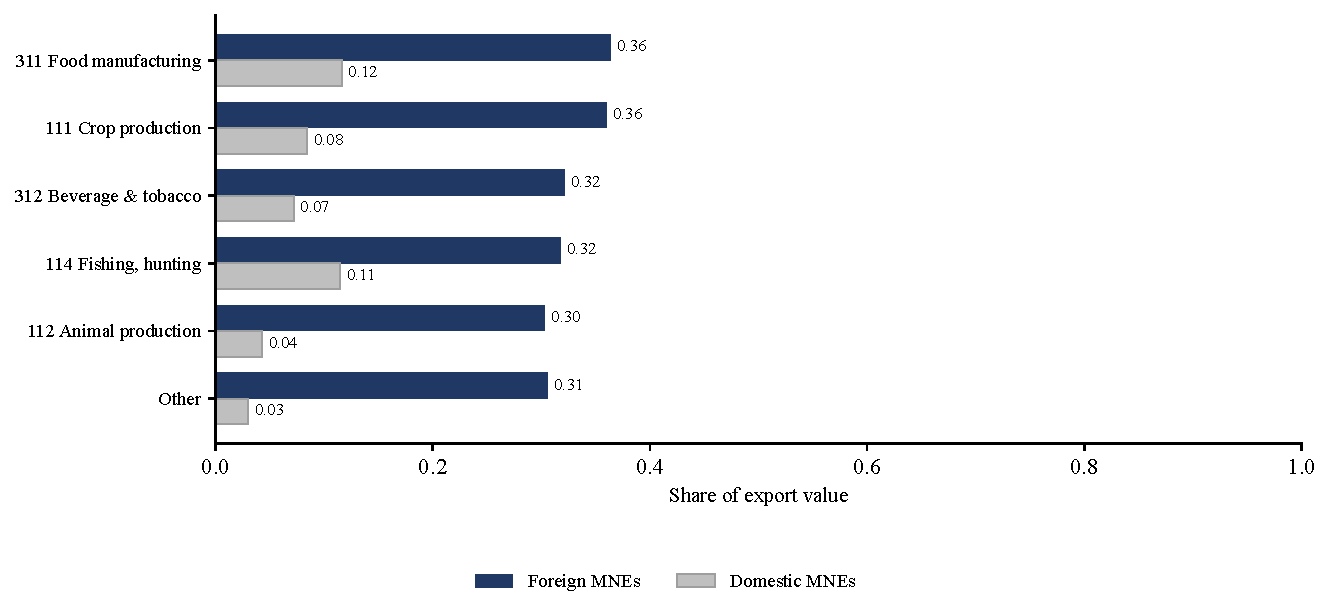
\includegraphics[width=0.9\textwidth,height=0.8\textheight,keepaspectratio]{figures/agro/fig_wp2_naics3.pdf}%
  \caption{Agriculture: Multinational Share of Export Value, by NAICS Industry}%
  \label{fig:sc_naics3_f_agro}%
  \par\vspace{2pt}%
  \parbox{0.92\textwidth}{\footnotesize %
  \textit{Notes:} Shares of agricultural export value (HS 01--24), all available years pooled. NAICS 3-digit industries assigned to HS6 products.\\[3pt]%
  \textit{Source:} Authors' calculations based on customs data matched to Orbis and Dun \& Bradstreet.}%
  \end{figure}
% ---- Figure: Agriculture: Foreign-Multinational Share of Export Value, by Exporting Country and NAICS Industry
\begin{figure}[H]\centering%
  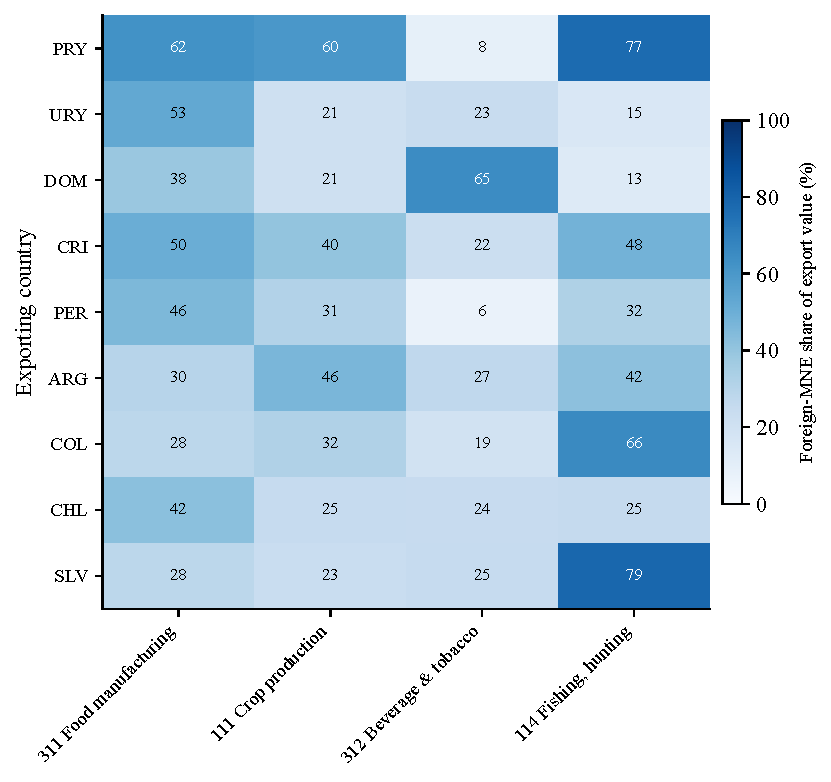
\includegraphics[width=0.95\textwidth,height=0.8\textheight,keepaspectratio]{figures/agro/fig_wp2_origin_x_naics3.pdf}%
  \caption{Agriculture: Foreign-Multinational Share of Export Value, by Exporting Country and NAICS Industry}%
  \label{fig:sc_naics3_hm_agro}%
  \par\vspace{2pt}%
  \parbox{0.92\textwidth}{\footnotesize %
  \textit{Notes:} Percent of each group's export value in each country shipped by foreign MNEs. NAICS 3-digit industries assigned to HS6 products.\\[3pt]%
  \textit{Source:} Authors' calculations based on customs data matched to Orbis and Dun \& Bradstreet.}%
  \end{figure}
% ---- Table: Agriculture: Exports by Exporting Country and NAICS Industry
\begin{table}[H]\centering\footnotesize%
  \caption{Agriculture: Exports by Exporting Country and NAICS Industry}%
  \label{tab:sc_naics3_ht_agro}%
  \adjustbox{max width=\textwidth, max totalheight=0.8\textheight}{\begin{tabular}{lrrrrrrr}
\toprule
Origin & 311 Food manufacturing & 111 Crop production & 312 Beverage \& tobacco & 114 Fishing, hunting & 112 Animal production & Other & All \\
\midrule
\multicolumn{8}{l}{\textit{Panel A: composition of the origin's exports, \% (rows sum to 100)}} \\
ARG & 74.8 & 20.7 & 3.2 & 0.2 & 0.7 & 0.4 & 100.0 \\
CHL & 34.3 & 36.8 & 18.3 & 9.7 & 0.3 & 0.7 & 100.0 \\
COL & 31.3 & 66.6 & 0.4 & 1.1 & 0.3 & 0.4 & 100.0 \\
CRI & 49.8 & 46.8 & 2.3 & 0.4 & 0.2 & 0.5 & 100.0 \\
DOM & 25.6 & 25.3 & 47.8 & 0.2 & 0.6 & 0.6 & 100.0 \\
PER & 23.1 & 46.7 & 1.4 & 28.0 & 0.1 & 0.6 & 100.0 \\
PRY & 82.9 & 15.4 & 1.5 & 0.1 & 0.0 & 0.0 & 100.0 \\
SLV & 60.1 & 26.8 & 10.4 & 0.7 & 1.7 & 0.2 & 100.0 \\
URY & 90.3 & 3.6 & 1.5 & 0.4 & 3.7 & 0.4 & 100.0 \\
All origins & 57.4 & 31.6 & 5.3 & 4.6 & 0.6 & 0.4 & 100.0 \\
\midrule
\multicolumn{8}{l}{\textit{Panel B: foreign-MNE share of export value, \%}} \\
ARG & 29.5 & 46.1 & 26.8 & 41.8 & 33.3 & 29.0 & 32.9 \\
CHL & 42.0 & 24.8 & 24.2 & 25.1 & 17.5 & 8.4 & 30.5 \\
COL & 28.0 & 31.9 & 19.4 & 65.6 & 2.4 & 12.0 & 30.9 \\
CRI & 50.1 & 39.9 & 22.2 & 48.0 & 17.9 & 34.3 & 44.6 \\
DOM & 38.5 & 20.6 & 64.5 & 12.8 & 1.4 & 88.8 & 46.4 \\
PER & 45.6 & 31.0 & 6.5 & 32.1 & 6.3 & 57.9 & 34.5 \\
PRY & 62.3 & 60.0 & 8.2 & 77.1 & 0.4 & 0.5 & 61.1 \\
SLV & 27.7 & 23.3 & 24.7 & 78.8 & 0.0 & 17.6 & 26.1 \\
URY & 52.5 & 21.1 & 23.5 & 15.1 & 43.3 & 35.3 & 50.4 \\
All origins & 36.4 & 36.0 & 32.1 & 31.8 & 30.3 & 30.6 & 35.8 \\
\bottomrule
\end{tabular}
}%
  \par\vspace{3pt}%
  \begin{minipage}{0.95\textwidth}\footnotesize %
  \textit{Notes:} Panel A: composition of each country's exports in the sector (rows add to 100). Panel B: percent of each cell's export value shipped by foreign MNEs. NAICS 3-digit industries assigned to HS6 products.\\[3pt]%
  \textit{Source:} Authors' calculations based on customs data matched to Orbis and Dun \& Bradstreet.%
  \end{minipage}%
  \end{table}
% ---- Table: Agriculture: Exports by NAICS Industry and Parent Country
\begin{table}[H]\centering\footnotesize%
  \caption{Agriculture: Exports by NAICS Industry and Parent Country}%
  \label{tab:sc_naics3_par_agro}%
  \adjustbox{max width=\textwidth, max totalheight=0.8\textheight}{\begin{tabular}{lrrrrrrrrrrrr}
\toprule
NAICS 3-digit (product-based) & USA & CHE & NLD & LIE & BRA & ESP & DEU & SAU & LUX & GBR & Other & Domestic \\
\midrule
311 Food manufacturing & 6.0 & 6.0 & 3.4 & 3.3 & 1.4 & 0.7 & 0.4 & 2.1 & 1.1 & 0.9 & 10.9 & 11.6 \\
111 Crop production & 7.5 & 2.1 & 2.2 & 1.7 & 0.8 & 1.4 & 4.1 & 0.1 & 0.2 & 0.3 & 15.7 & 8.4 \\
312 Beverage \& tobacco & 3.3 & 0.6 & 0.6 & 0.1 & 0.0 & 0.9 & 0.1 & 0.0 & 2.7 & 3.3 & 20.6 & 7.2 \\
114 Fishing, hunting & 1.6 & 0.0 & 0.3 & 0.0 & 0.0 & 0.2 & 0.1 & 0.0 & 0.2 & 4.9 & 24.4 & 11.5 \\
112 Animal production & 0.1 & 0.0 & 2.3 & 0.0 & 0.0 & 0.3 & 0.0 & 0.3 & 0.0 & 0.6 & 26.6 & 4.3 \\
Other & 4.2 & 1.2 & 1.0 & 1.9 & 0.1 & 0.5 & 0.3 & 0.0 & 0.0 & 2.9 & 18.6 & 3.0 \\
\bottomrule
\end{tabular}
}%
  \par\vspace{3pt}%
  \begin{minipage}{0.95\textwidth}\footnotesize %
  \textit{Notes:} Percent of each group's export value, by country of the ultimate parent of foreign MNEs; domestic MNEs shown for comparison. NAICS 3-digit industries assigned to HS6 products.\\[3pt]%
  \textit{Source:} Authors' calculations based on customs data matched to Orbis and Dun \& Bradstreet.%
  \end{minipage}%
  \end{table}

\subsection{By Technology Class}
% ---- Table: Agriculture: Exports and Multinational Shares, by Technology Class
\begin{table}[H]\centering\footnotesize%
  \caption{Agriculture: Exports and Multinational Shares, by Technology Class}%
  \label{tab:sc_lall2000_category_agro}%
  \adjustbox{max width=\textwidth, max totalheight=0.8\textheight}{\begin{tabular}{@{}l r r r r l@{}}
\toprule
Lall (2000) category & Total exports (US\$bn/yr) & MNE exports (US\$bn/yr) & Foreign (\%) & Domestic (\%) & Leading parents (share of foreign) \\
\midrule
Primary products & 27.3 & 14.9 & 45.9 & 7.9 & USA 0.34, NLD 0.11, CHE 0.09 \\
Resource-based manufactures: agro-based & 20.6 & 9.6 & 37.7 & 9.5 & USA 0.18, SAU 0.10, CHE 0.09 \\
Medium technology manufactures: engineering & 16.1 & 7.5 & 33.3 & 13.5 & CHE 0.25, LIE 0.17, USA 0.14 \\
Medium technology manufactures: process & 6.9 & 2.5 & 29.8 & 6.6 & USA 0.19, ESP 0.15, JOR 0.13 \\
Low technology manufactures: textile, garment and footwear & 0.7 & 0.2 & 16.4 & 6.8 & USA 0.67, LIE 0.26, COL 0.06 \\
Resource-based manufactures: other & 0.6 & 0.2 & 25.3 & 10.1 & BMU 0.24, PAN 0.18, USA 0.13 \\
High technology manufactures: other & 0.5 & 0.1 & 23.8 & 3.1 & ITA 0.17, DEU 0.16, SGP 0.15 \\
High technology manufactures: electronic and electrical & 0.1 & 0.0 & 20.3 & 0.9 & KOR 0.33, SLV 0.19, CHE 0.10 \\
\midrule
All & 72.9 & 35.0 & 38.5 & 9.4 & \\
\bottomrule
\end{tabular}
}%
  \par\vspace{3pt}%
  \begin{minipage}{0.95\textwidth}\footnotesize %
  \textit{Notes:} Lall (2000) technology classes. Foreign and domestic: percent of the group's export value. Leading parents: the three largest parent countries and their share of the row's foreign-MNE exports. Values are annual averages in US\$ billion.\\[3pt]%
  \textit{Source:} Authors' calculations based on customs data matched to Orbis and Dun \& Bradstreet.%
  \end{minipage}%
  \end{table}
% ---- Figure: Agriculture: Multinational Share of Export Value, by Technology Class
\begin{figure}[H]\centering%
  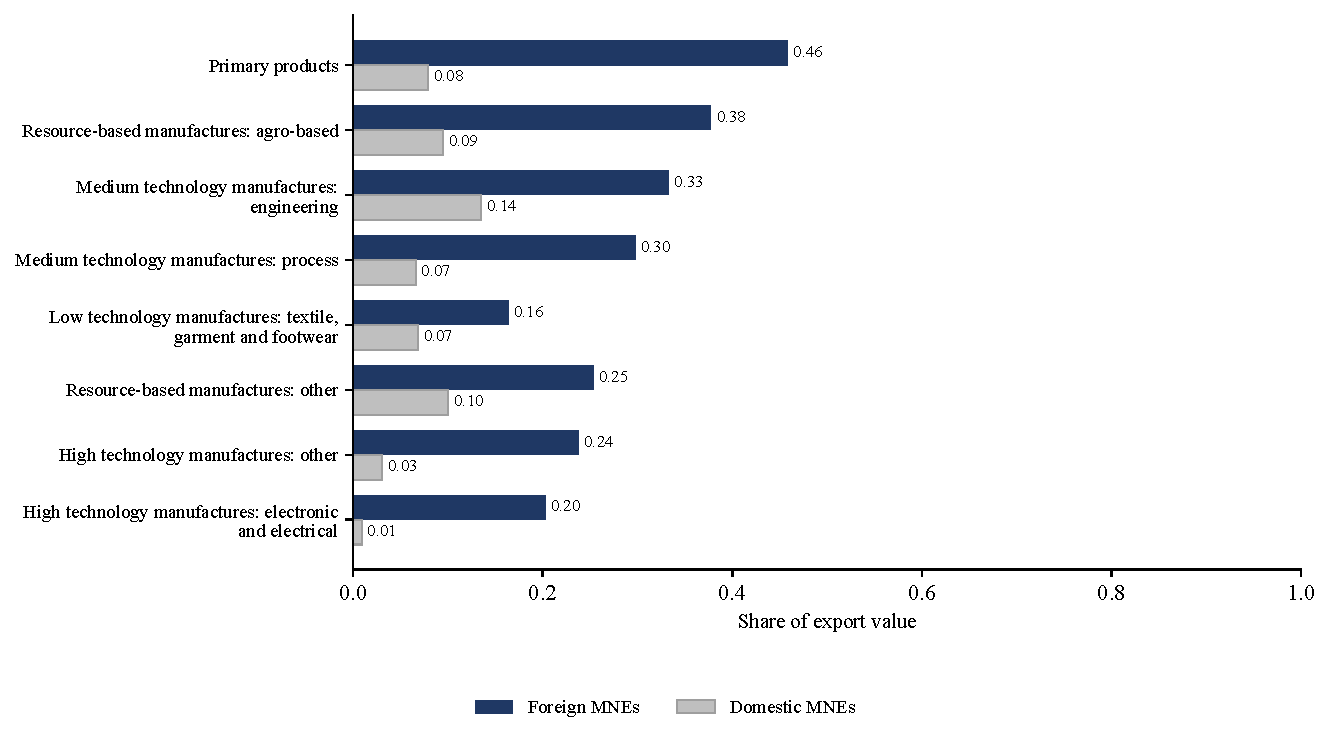
\includegraphics[width=0.9\textwidth,height=0.8\textheight,keepaspectratio]{figures/agro/fig_wp2_lall2000_category.pdf}%
  \caption{Agriculture: Multinational Share of Export Value, by Technology Class}%
  \label{fig:sc_lall2000_category_f_agro}%
  \par\vspace{2pt}%
  \parbox{0.92\textwidth}{\footnotesize %
  \textit{Notes:} Shares of agricultural export value (HS 01--24), all available years pooled. Lall (2000) technology classes.\\[3pt]%
  \textit{Source:} Authors' calculations based on customs data matched to Orbis and Dun \& Bradstreet.}%
  \end{figure}
% ---- Figure: Agriculture: Foreign-Multinational Share of Export Value, by Exporting Country and Technology Class
\begin{figure}[H]\centering%
  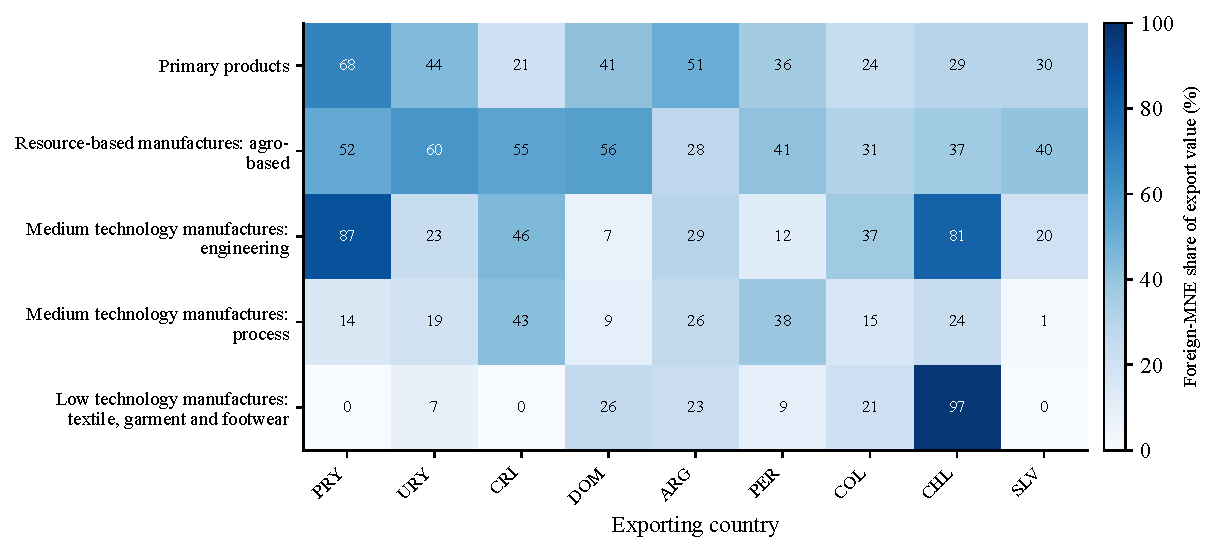
\includegraphics[width=0.95\textwidth,height=0.8\textheight,keepaspectratio]{figures/agro/fig_wp2_origin_x_lall2000_category.pdf}%
  \caption{Agriculture: Foreign-Multinational Share of Export Value, by Exporting Country and Technology Class}%
  \label{fig:sc_lall2000_category_hm_agro}%
  \par\vspace{2pt}%
  \parbox{0.92\textwidth}{\footnotesize %
  \textit{Notes:} Percent of each group's export value in each country shipped by foreign MNEs. Lall (2000) technology classes.\\[3pt]%
  \textit{Source:} Authors' calculations based on customs data matched to Orbis and Dun \& Bradstreet.}%
  \end{figure}
% ---- Table: Agriculture: Exports by Exporting Country and Technology Class
\begin{table}[H]\centering\footnotesize%
  \caption{Agriculture: Exports by Exporting Country and Technology Class}%
  \label{tab:sc_lall2000_category_ht_agro}%
  \adjustbox{max width=\textwidth, max totalheight=0.8\textheight}{\begin{tabular}{lrrrrrrrrrr}
\toprule
Sub-sector & ARG & CHL & COL & CRI & DOM & PER & PRY & SLV & URY & All \\
\midrule
\multicolumn{11}{l}{\textit{Panel A: composition of the origin's exports, \% (columns sum to 100)}} \\
Primary products & 39.4 & 28.3 & 26.9 & 13.3 & 11.4 & 42.4 & 52.6 & 9.2 & 55.0 & 36.8 \\
Resource-based manufactures: agro-based & 27.3 & 34.6 & 18.7 & 38.0 & 57.6 & 15.1 & 28.6 & 56.0 & 41.4 & 28.3 \\
Medium technology manufactures: engineering & 28.4 & 0.6 & 43.8 & 9.6 & 10.6 & 12.9 & 16.3 & 21.4 & 0.4 & 21.6 \\
Medium technology manufactures: process & 3.4 & 35.2 & 4.7 & 38.2 & 14.6 & 22.4 & 0.6 & 6.3 & 1.9 & 10.5 \\
Low technology manufactures: textile, garment and footwear & 0.3 & 0.0 & 4.8 & 0.6 & 5.2 & 0.7 & 1.1 & 6.5 & 0.0 & 1.0 \\
Resource-based manufactures: other & 0.1 & 1.2 & 0.1 & 0.0 & 0.0 & 4.5 & 0.8 & 0.1 & 1.3 & 0.8 \\
High technology manufactures: other & 1.1 & 0.1 & 0.9 & 0.2 & 0.6 & 0.5 & 0.0 & 0.4 & 0.0 & 0.7 \\
High technology manufactures: electronic and electrical & 0.0 & 0.0 & 0.1 & 0.1 & 0.0 & 1.5 & 0.0 & 0.1 & 0.0 & 0.2 \\
All sub-sectors & 100.0 & 100.0 & 100.0 & 100.0 & 100.0 & 100.0 & 100.0 & 100.0 & 100.0 & 100.0 \\
\midrule
\multicolumn{11}{l}{\textit{Panel B: foreign-MNE share of export value, \%}} \\
Primary products & 50.8 & 29.3 & 23.8 & 20.5 & 41.2 & 35.9 & 67.8 & 29.8 & 44.4 & 45.9 \\
Resource-based manufactures: agro-based & 27.7 & 36.6 & 31.0 & 54.6 & 56.4 & 41.0 & 52.3 & 39.9 & 60.4 & 37.7 \\
Medium technology manufactures: engineering & 29.5 & 80.8 & 37.1 & 45.7 & 6.8 & 11.6 & 86.8 & 20.2 & 23.5 & 33.3 \\
Medium technology manufactures: process & 26.4 & 24.2 & 15.4 & 42.9 & 9.3 & 37.9 & 14.4 & 0.9 & 19.4 & 29.8 \\
Low technology manufactures: textile, garment and footwear & 22.8 & 96.9 & 20.9 & 0.0 & 26.0 & 9.0 & 0.0 & 0.0 & 7.4 & 16.4 \\
Resource-based manufactures: other & 29.9 & 22.7 & 91.7 & 41.7 & 75.4 & 25.2 & 18.9 & 36.1 & 21.2 & 25.3 \\
High technology manufactures: other & 26.3 & 37.3 & 14.4 & 52.2 & 4.1 & 14.0 & 25.4 & 18.7 & 34.9 & 23.8 \\
High technology manufactures: electronic and electrical & 22.6 & 27.0 & 17.2 & 38.7 & 26.1 & 19.7 & 13.9 & 41.6 & 16.7 & 20.3 \\
All sub-sectors & 37.2 & 30.3 & 30.4 & 44.4 & 40.7 & 33.0 & 65.0 & 29.6 & 50.2 & 38.5 \\
\bottomrule
\end{tabular}
}%
  \par\vspace{3pt}%
  \begin{minipage}{0.95\textwidth}\footnotesize %
  \textit{Notes:} Panel A: composition of each country's exports in the sector (rows add to 100). Panel B: percent of each cell's export value shipped by foreign MNEs. Lall (2000) technology classes.\\[3pt]%
  \textit{Source:} Authors' calculations based on customs data matched to Orbis and Dun \& Bradstreet.%
  \end{minipage}%
  \end{table}
% ---- Table: Agriculture: Exports by Technology Class and Parent Country
\begin{table}[H]\centering\footnotesize%
  \caption{Agriculture: Exports by Technology Class and Parent Country}%
  \label{tab:sc_lall2000_category_par_agro}%
  \adjustbox{max width=\textwidth, max totalheight=0.8\textheight}{\begin{tabular}{lrrrrrrrrrrrr}
\toprule
Lall (2000) category & USA & CHE & NLD & LIE & BRA & ESP & DEU & SAU & LUX & GBR & Other & Domestic \\
\midrule
Primary products & 13.8 & 3.7 & 4.5 & 3.3 & 1.4 & 1.8 & 0.6 & 0.3 & 0.9 & 1.0 & 14.5 & 7.9 \\
Resource-based manufactures: agro-based & 5.9 & 3.1 & 2.2 & 1.2 & 1.8 & 0.9 & 0.5 & 3.2 & 2.1 & 1.4 & 15.5 & 9.5 \\
Medium technology manufactures: engineering & 4.5 & 7.9 & 3.8 & 5.4 & 0.7 & 0.1 & 3.8 & 0.1 & 0.0 & 0.3 & 6.8 & 13.5 \\
Medium technology manufactures: process & 4.3 & 0.2 & 0.7 & 0.1 & 0.0 & 3.3 & 0.5 & 0.0 & 0.7 & 0.6 & 19.3 & 6.6 \\
Low technology manufactures: textile, garment and footwear & 7.2 & 0.0 & 0.0 & 2.8 & 0.0 & 0.0 & 0.0 & 0.0 & 0.0 & 0.0 & 6.4 & 6.8 \\
Resource-based manufactures: other & 3.0 & 0.0 & 1.6 & 0.0 & 0.4 & 0.0 & 1.6 & 1.2 & 0.0 & 2.9 & 14.6 & 10.1 \\
High technology manufactures: other & 0.6 & 0.1 & 0.0 & 0.0 & 0.1 & 0.2 & 2.3 & 0.0 & 0.0 & 0.0 & 20.5 & 3.1 \\
High technology manufactures: electronic and electrical & 0.5 & 1.2 & 0.0 & 0.0 & 0.0 & 0.2 & 0.1 & 0.0 & 0.0 & 0.0 & 18.1 & 0.9 \\
\bottomrule
\end{tabular}
}%
  \par\vspace{3pt}%
  \begin{minipage}{0.95\textwidth}\footnotesize %
  \textit{Notes:} Percent of each group's export value, by country of the ultimate parent of foreign MNEs; domestic MNEs shown for comparison. Lall (2000) technology classes.\\[3pt]%
  \textit{Source:} Authors' calculations based on customs data matched to Orbis and Dun \& Bradstreet.%
  \end{minipage}%
  \end{table}

\subsection{By Inputs and Other Products}
% ---- Table: Agriculture: Exports and Multinational Shares, by Inputs and Other Products
\begin{table}[H]\centering\footnotesize%
  \caption{Agriculture: Exports and Multinational Shares, by Inputs and Other Products}%
  \label{tab:sc_inputs_agro}%
  \adjustbox{max width=\textwidth, max totalheight=0.8\textheight}{\begin{tabular}{@{}l r r r r l@{}}
\toprule
Inputs vs output & Total exports (US\$bn/yr) & MNE exports (US\$bn/yr) & Foreign (\%) & Domestic (\%) & Leading parents (share of foreign) \\
\midrule
Agricultural inputs & 14.9 & 7.0 & 36.0 & 10.8 & CHE 0.26, LIE 0.18, USA 0.18 \\
Agricultural output (food, fibres, beverages) & 64.0 & 30.8 & 38.6 & 9.2 & USA 0.25, NLD 0.09, CHE 0.08 \\
\midrule
All & 78.9 & 37.8 & 38.1 & 9.5 & \\
\bottomrule
\end{tabular}
}%
  \par\vspace{3pt}%
  \begin{minipage}{0.95\textwidth}\footnotesize %
  \textit{Notes:} Inputs: seeds, animal feed and live animals. Foreign and domestic: percent of the group's export value. Leading parents: the three largest parent countries and their share of the row's foreign-MNE exports. Values are annual averages in US\$ billion.\\[3pt]%
  \textit{Source:} Authors' calculations based on customs data matched to Orbis and Dun \& Bradstreet.%
  \end{minipage}%
  \end{table}
% ---- Figure: Agriculture: Multinational Share of Export Value, by Inputs and Other Products
\begin{figure}[H]\centering%
  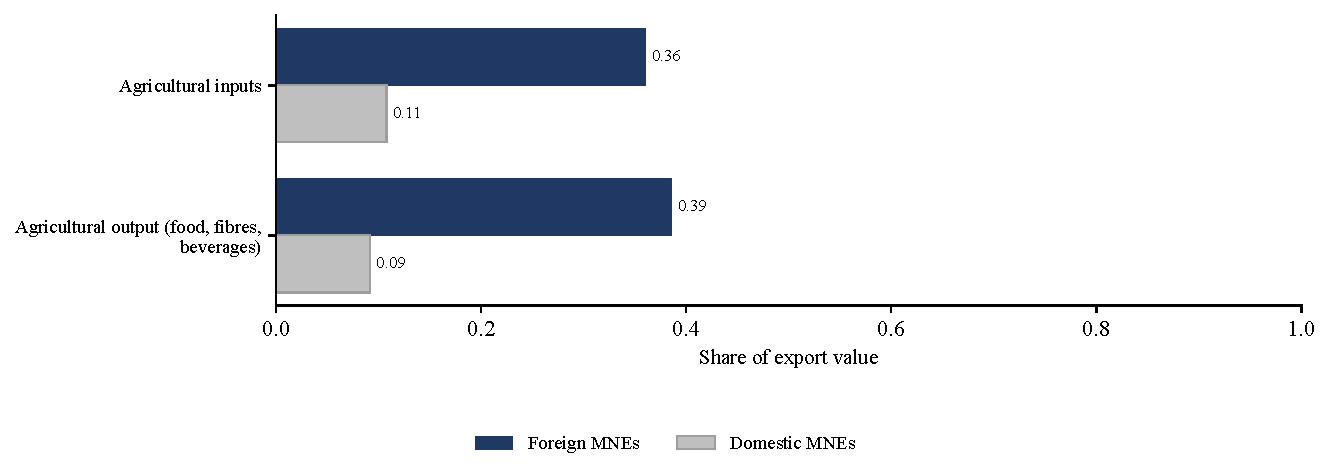
\includegraphics[width=0.9\textwidth,height=0.8\textheight,keepaspectratio]{figures/agro/fig_wp2_inputs.pdf}%
  \caption{Agriculture: Multinational Share of Export Value, by Inputs and Other Products}%
  \label{fig:sc_inputs_f_agro}%
  \par\vspace{2pt}%
  \parbox{0.92\textwidth}{\footnotesize %
  \textit{Notes:} Shares of agricultural export value (HS 01--24), all available years pooled. Inputs: seeds, animal feed and live animals.\\[3pt]%
  \textit{Source:} Authors' calculations based on customs data matched to Orbis and Dun \& Bradstreet.}%
  \end{figure}
% ---- Figure: Agriculture: Foreign-Multinational Share of Export Value, by Exporting Country and Inputs and Other Products
\begin{figure}[H]\centering%
  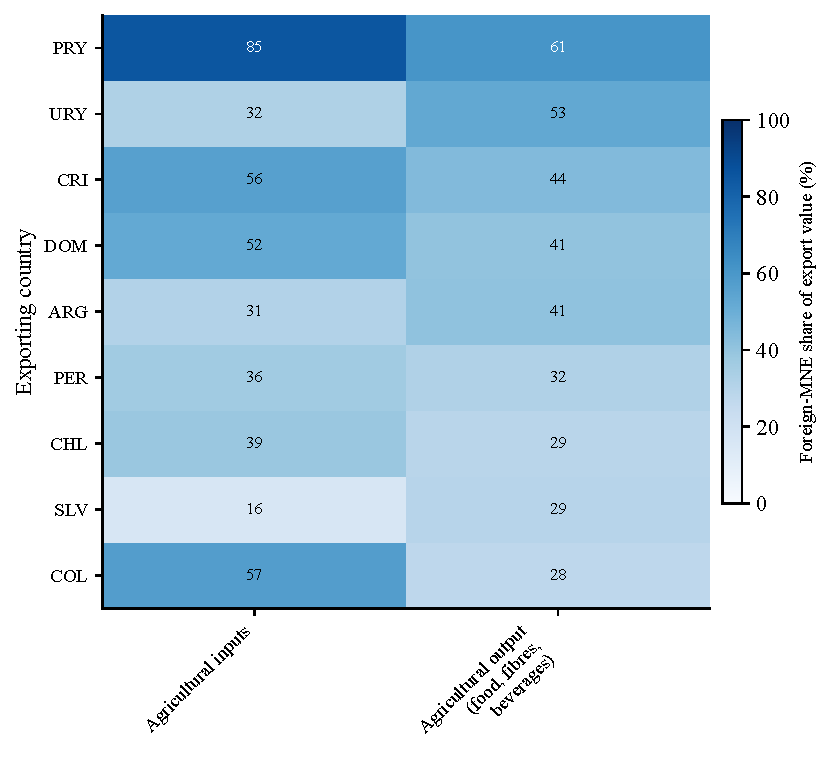
\includegraphics[width=0.95\textwidth,height=0.8\textheight,keepaspectratio]{figures/agro/fig_wp2_origin_x_inputs.pdf}%
  \caption{Agriculture: Foreign-Multinational Share of Export Value, by Exporting Country and Inputs and Other Products}%
  \label{fig:sc_inputs_hm_agro}%
  \par\vspace{2pt}%
  \parbox{0.92\textwidth}{\footnotesize %
  \textit{Notes:} Percent of each group's export value in each country shipped by foreign MNEs. Inputs: seeds, animal feed and live animals.\\[3pt]%
  \textit{Source:} Authors' calculations based on customs data matched to Orbis and Dun \& Bradstreet.}%
  \end{figure}
% ---- Table: Agriculture: Exports by Exporting Country and Inputs and Other Products
\begin{table}[H]\centering\footnotesize%
  \caption{Agriculture: Exports by Exporting Country and Inputs and Other Products}%
  \label{tab:sc_inputs_ht_agro}%
  \adjustbox{max width=\textwidth, max totalheight=0.8\textheight}{\begin{tabular}{lrrr}
\toprule
Origin & Agricultural inputs & Agricultural output (food, fibres, beverages) & All \\
\midrule
\multicolumn{4}{l}{\textit{Panel A: composition of the origin's exports, \% (rows sum to 100)}} \\
ARG & 29.9 & 70.1 & 100.0 \\
CHL & 5.0 & 95.0 & 100.0 \\
COL & 0.9 & 99.1 & 100.0 \\
CRI & 1.7 & 98.3 & 100.0 \\
DOM & 1.3 & 98.7 & 100.0 \\
PER & 21.7 & 78.3 & 100.0 \\
PRY & 17.0 & 83.0 & 100.0 \\
SLV & 2.8 & 97.2 & 100.0 \\
URY & 3.4 & 96.6 & 100.0 \\
All origins & 17.5 & 82.5 & 100.0 \\
\midrule
\multicolumn{4}{l}{\textit{Panel B: foreign-MNE share of export value, \%}} \\
ARG & 31.1 & 40.7 & 37.8 \\
CHL & 38.7 & 29.2 & 29.6 \\
COL & 57.1 & 27.7 & 28.0 \\
CRI & 56.2 & 44.3 & 44.5 \\
DOM & 52.0 & 40.5 & 40.7 \\
PER & 36.4 & 32.0 & 33.0 \\
PRY & 85.4 & 60.8 & 65.0 \\
SLV & 15.7 & 29.3 & 28.9 \\
URY & 32.3 & 52.5 & 51.8 \\
All origins & 36.0 & 38.6 & 38.1 \\
\bottomrule
\end{tabular}
}%
  \par\vspace{3pt}%
  \begin{minipage}{0.95\textwidth}\footnotesize %
  \textit{Notes:} Panel A: composition of each country's exports in the sector (rows add to 100). Panel B: percent of each cell's export value shipped by foreign MNEs. Inputs: seeds, animal feed and live animals.\\[3pt]%
  \textit{Source:} Authors' calculations based on customs data matched to Orbis and Dun \& Bradstreet.%
  \end{minipage}%
  \end{table}
% ---- Table: Agriculture: Exports by Inputs and Other Products and Parent Country
\begin{table}[H]\centering\footnotesize%
  \caption{Agriculture: Exports by Inputs and Other Products and Parent Country}%
  \label{tab:sc_inputs_par_agro}%
  \adjustbox{max width=\textwidth, max totalheight=0.8\textheight}{\begin{tabular}{lrrrrrrrrrrrr}
\toprule
Inputs vs output & USA & CHE & NLD & LIE & BRA & ESP & DEU & SAU & LUX & GBR & Other & Domestic \\
\midrule
Agricultural inputs & 6.0 & 9.0 & 4.4 & 6.1 & 0.3 & 0.4 & 1.0 & 0.1 & 0.0 & 1.1 & 7.6 & 10.8 \\
Agricultural output (food, fibres, beverages) & 8.4 & 2.6 & 2.9 & 1.8 & 1.5 & 1.4 & 1.2 & 1.3 & 1.2 & 0.8 & 15.4 & 9.2 \\
\bottomrule
\end{tabular}
}%
  \par\vspace{3pt}%
  \begin{minipage}{0.95\textwidth}\footnotesize %
  \textit{Notes:} Percent of each group's export value, by country of the ultimate parent of foreign MNEs; domestic MNEs shown for comparison. Inputs: seeds, animal feed and live animals.\\[3pt]%
  \textit{Source:} Authors' calculations based on customs data matched to Orbis and Dun \& Bradstreet.%
  \end{minipage}%
  \end{table}
% ---- Table: Agriculture: Largest Input Products
\begin{table}[H]\centering\footnotesize%
  \caption{Agriculture: Largest Input Products}%
  \label{tab:sc_topin_agro}%
  \adjustbox{max width=\textwidth, max totalheight=0.8\textheight}{\begin{tabular}{@{}l p{7.5cm} r r r@{}}
\toprule
HS6 & Description & \$bn/yr & Foreign (\%) & Domestic (\%) \\
\midrule
230400 & Oil-cake \& other solid residues, whether/not ground/in pellets, from extraction of soyabean oil & 10.84 & 35 & 12 \\
230120 & Flours, meals \& pellets of fish/of crustaceans, molluscs/other aquatic invertebrates & 1.70 & 31 & 10 \\
230990 & Preparations of a kind used in animal feeding other than dog/cat food put up for RS & 0.51 & 57 & 3 \\
071333 & Kidney beans, incl. white pea beans (Phaseolus vulgaris), dried, shelled, whether/not skinned/split & 0.30 & 28 & 4 \\
230250 & Bran, sharps \& other residues, whether/not in the form of pellets, derived from the sifting/milling/other working of leguminous plants & 0.28 & 30 & 16 \\
100510 & Maize (corn), seed & 0.19 & 60 & 3 \\
230910 & Dog/cat food, put up for RS & 0.17 & 81 & 5 \\
120991 & Vegetable seeds, of a kind used for sowing & 0.12 & 67 & 1 \\
230630 & Oil-cake \& other solid residues, whether/not ground/in pellets, from extraction of sunflower seeds & 0.12 & 22 & 2 \\
010290 & Live bovine animals other than pure-bred breeding animals & 0.08 & 31 & 0 \\
071320 & Chickpeas (garbanzos), dried, shelled, whether/not skinned/split & 0.08 & 23 & 2 \\
230800 & Vegetable materials/waste/residues/by-products, whether/not in pellets, of a kind used in animal feeding, n.e.s. & 0.08 & 19 & 0 \\
100610 & Rice in the husk (paddy/rough) & 0.06 & 45 & 5 \\
230110 & Flours, meals \& pellets of meat/meat offal; greaves & 0.05 & 31 & 0 \\
051199 & Animal products not elsewhere specified/incld. (excl. of 0511.10); dead animals of Ch. 1, unfit for human consumption & 0.04 & 39 & 5 \\
071310 & Peas (Pisum sativum), dried, shelled, whether/not skinned/split & 0.03 & 22 & 1 \\
071339 & Beans (Vigna spp., Phaseolus spp. (excl. of 0713.31-0713.33)), dried, shelled, whether/not skinned/split & 0.03 & 11 & 2 \\
230230 & Bran, sharps \& other residues, whether/not in the form of pellets, derived from the sifting/milling/other working of wheat & 0.03 & 16 & 1 \\
010511 & Live fowls of species Gallus domesticus, weighing not >185g & 0.02 & 3 & 1 \\
120930 & Seeds of herbaceous plants cultivated principally for their flowers, of a kind used for sowing & 0.02 & 76 & 2 \\
\bottomrule
\end{tabular}
}%
  \par\vspace{3pt}%
  \begin{minipage}{0.95\textwidth}\footnotesize %
  \textit{Notes:} HS6 input products with the largest export value. Foreign and domestic: percent of the product's export value. Values are annual averages in US\$ billion.\\[3pt]%
  \textit{Source:} Authors' calculations based on customs data matched to Orbis and Dun \& Bradstreet.%
  \end{minipage}%
  \end{table}

\subsection{HS Section and End Use}
% ---- Table: Agriculture: Exports by HS Section and End Use
\begin{table}[H]\centering\small%
  \caption{Agriculture: Exports by HS Section and End Use}%
  \label{tab:sxe_v_agro}%
  \adjustbox{max width=\textwidth, max totalheight=0.8\textheight}{\begin{tabular}{lrrrr}
\toprule
HS section / BEC end use & Intermediate & Consumption & Capital & Total \\
\midrule
I Live animals; animal products & 0.8 & 9.6 & 0.0 & 10.4 \\
II Vegetable products & 20.0 & 10.6 & 0.0 & 30.6 \\
III Fats and oils & 6.3 & 0.6 & 0.0 & 6.9 \\
IV Prepared foodstuffs, beverages, tobacco & 15.4 & 9.6 & 0.0 & 25.0 \\
\midrule
Total & 42.5 & 30.4 & 0.0 & 72.9 \\
\bottomrule
\end{tabular}
}%
  \par\vspace{3pt}%
  \begin{minipage}{0.95\textwidth}\footnotesize %
  \textit{Notes:} Export value by HS section and BEC Rev.\,4 end use. Values are annual averages in US\$ billion.\\[3pt]%
  \textit{Source:} Authors' calculations based on customs data matched to Orbis and Dun \& Bradstreet.%
  \end{minipage}%
  \end{table}
% ---- Table: Agriculture: Foreign-Multinational Share of Exports by HS Section and End Use
\begin{table}[H]\centering\small%
  \caption{Agriculture: Foreign-Multinational Share of Exports by HS Section and End Use}%
  \label{tab:sxe_f_agro}%
  \adjustbox{max width=\textwidth, max totalheight=0.8\textheight}{\begin{tabular}{lrrr}
\toprule
HS section / BEC end use & Intermediate & Consumption & Capital \\
\midrule
I Live animals; animal products & 33.1 & 35.8 & 16.8 \\
II Vegetable products & 50.2 & 28.3 & -- \\
III Fats and oils & 29.8 & 47.0 & -- \\
IV Prepared foodstuffs, beverages, tobacco & 33.9 & 41.6 & -- \\
\bottomrule
\end{tabular}
}%
  \par\vspace{3pt}%
  \begin{minipage}{0.95\textwidth}\footnotesize %
  \textit{Notes:} Percent of each cell's export value shipped by foreign MNEs.\\[3pt]%
  \textit{Source:} Authors' calculations based on customs data matched to Orbis and Dun \& Bradstreet.%
  \end{minipage}%
  \end{table}
\clearpage\part{Manufacturing}

\section{Fact 1: Multinationals Account for a Large Share of Exports}\label{sec:f1_manufacturing}
% ---- Figure: Manufacturing: Multinational Share of Export Value, by Exporting Country
\begin{figure}[H]\centering%
  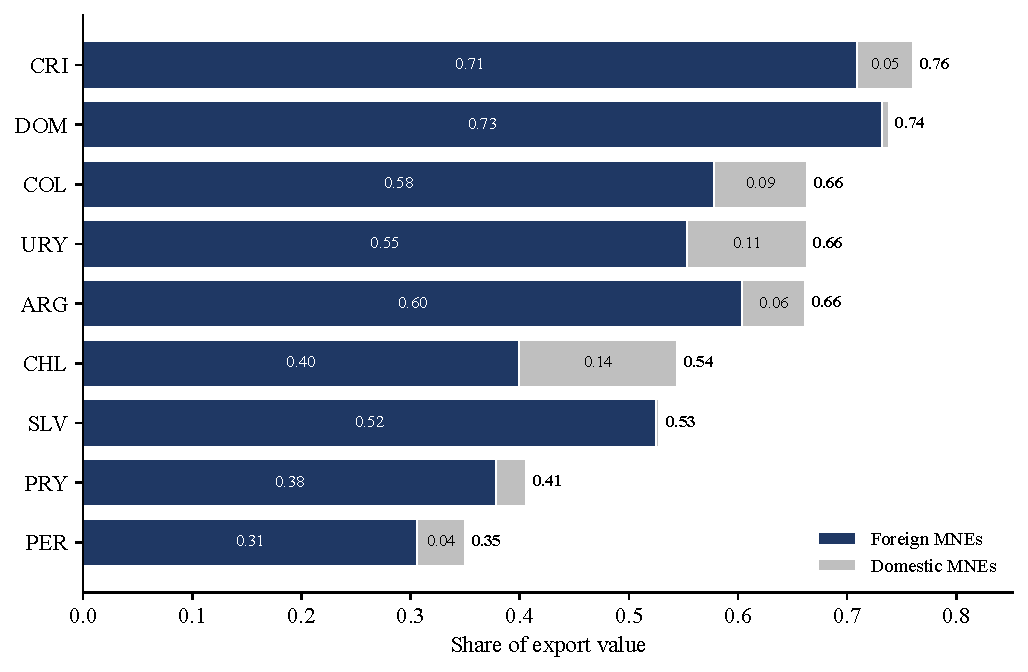
\includegraphics[width=0.8\textwidth,height=0.8\textheight,keepaspectratio]{figures/manufacturing/fig_wp0_fig1_origin.pdf}%
  \caption{Manufacturing: Multinational Share of Export Value, by Exporting Country}%
  \label{fig:f1_manufacturing}%
  \par\vspace{2pt}%
  \parbox{0.92\textwidth}{\footnotesize %
  \textit{Notes:} Shares of manufacturing export value (HS 28--97 excluding 71), all available years pooled. The figure at the end of each bar is the total MNE share.\\[3pt]%
  \textit{Source:} Authors' calculations based on customs data matched to Orbis and Dun \& Bradstreet.}%
  \end{figure}
% ---- Table: Manufacturing: Multinational Share of Export Value, by Exporting Country
\begin{table}[H]\centering\small%
  \caption{Manufacturing: Multinational Share of Export Value, by Exporting Country}%
  \label{tab:f1n_manufacturing}%
  \adjustbox{max width=\textwidth, max totalheight=0.8\textheight}{\begin{tabular}{lrrrr}
\toprule
Origin & Foreign & Domestic & All MNEs & Value (US\$bn/yr) \\
\midrule
CRI & 0.709 & 0.052 & 0.761 & 6.0 \\
DOM & 0.732 & 0.006 & 0.738 & 4.7 \\
COL & 0.578 & 0.086 & 0.663 & 8.9 \\
URY & 0.553 & 0.110 & 0.663 & 2.4 \\
ARG & 0.604 & 0.058 & 0.662 & 21.7 \\
CHL & 0.399 & 0.145 & 0.544 & 16.0 \\
SLV & 0.525 & 0.004 & 0.528 & 3.8 \\
PRY & 0.379 & 0.027 & 0.406 & 1.0 \\
PER & 0.306 & 0.044 & 0.350 & 8.1 \\
\midrule
All & 0.516 & 0.080 & 0.596 & 72.7 \\
\bottomrule
\end{tabular}
}%
  \par\vspace{3pt}%
  \begin{minipage}{0.95\textwidth}\footnotesize %
  \textit{Notes:} Shares of manufacturing export value (HS 28--97 excluding 71), all available years pooled. Values are annual averages in US\$ billion.\\[3pt]%
  \textit{Source:} Authors' calculations based on customs data matched to Orbis and Dun \& Bradstreet.%
  \end{minipage}%
  \end{table}

\subsection{By Parent Country}
% ---- Figure: Manufacturing: Multinational Share of Export Value, by Exporting Country and Parent Country
\begin{figure}[H]\centering%
  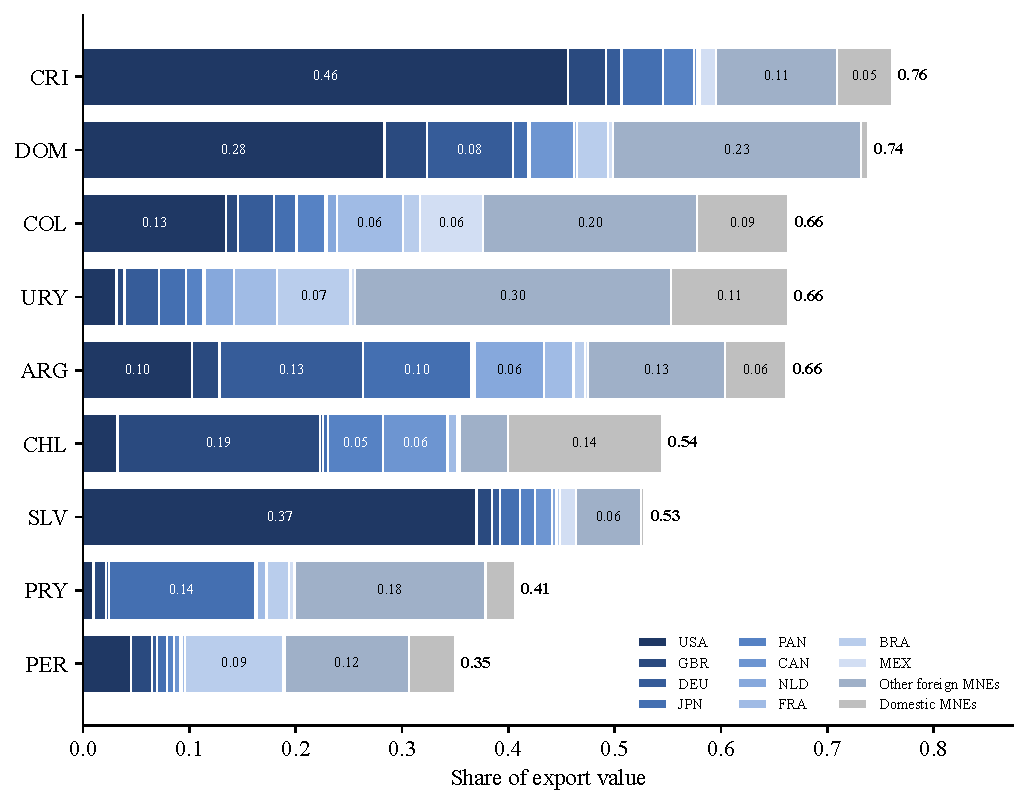
\includegraphics[width=0.92\textwidth,height=0.8\textheight,keepaspectratio]{figures/manufacturing/fig_wp1a_origin_by_parent.pdf}%
  \caption{Manufacturing: Multinational Share of Export Value, by Exporting Country and Parent Country}%
  \label{fig:f1p_manufacturing}%
  \par\vspace{2pt}%
  \parbox{0.92\textwidth}{\footnotesize %
  \textit{Notes:} Shares of manufacturing export value (HS 28--97 excluding 71), all available years pooled. Foreign MNEs split by country of the ultimate parent; the ten largest parent countries are shown separately.\\[3pt]%
  \textit{Source:} Authors' calculations based on customs data matched to Orbis and Dun \& Bradstreet.}%
  \end{figure}
% ---- Table: Manufacturing: Multinational Share of Export Value, by Exporting Country and Parent Country
\begin{table}[H]\centering\small%
  \caption{Manufacturing: Multinational Share of Export Value, by Exporting Country and Parent Country}%
  \label{tab:f1pn_manufacturing}%
  \adjustbox{max width=\textwidth, max totalheight=0.8\textheight}{\begin{tabular}{lcccccccccccccc}
\toprule
Origin & USA & GBR & DEU & JPN & PAN & CAN & NLD & FRA & BRA & MEX & Other & Domestic & All MNEs & Value (US\$bn/yr) \\
\midrule
CRI & 0.456 & 0.036 & 0.015 & 0.039 & 0.029 & 0.003 & 0.001 & 0.001 & 0.000 & 0.015 & 0.113 & 0.052 & 0.761 & 6.0 \\
DOM & 0.284 & 0.040 & 0.081 & 0.014 & 0.002 & 0.041 & 0.000 & 0.003 & 0.029 & 0.005 & 0.233 & 0.006 & 0.738 & 4.7 \\
COL & 0.135 & 0.011 & 0.034 & 0.021 & 0.027 & 0.002 & 0.010 & 0.063 & 0.016 & 0.060 & 0.201 & 0.086 & 0.663 & 8.9 \\
URY & 0.031 & 0.008 & 0.032 & 0.025 & 0.016 & 0.001 & 0.028 & 0.040 & 0.069 & 0.004 & 0.298 & 0.110 & 0.663 & 2.4 \\
ARG & 0.102 & 0.026 & 0.135 & 0.102 & 0.001 & 0.002 & 0.065 & 0.028 & 0.011 & 0.003 & 0.129 & 0.058 & 0.662 & 21.7 \\
CHL & 0.032 & 0.191 & 0.003 & 0.004 & 0.052 & 0.060 & 0.001 & 0.008 & 0.002 & 0.001 & 0.045 & 0.145 & 0.544 & 16.0 \\
SLV & 0.370 & 0.015 & 0.007 & 0.019 & 0.014 & 0.015 & 0.004 & 0.001 & 0.003 & 0.015 & 0.061 & 0.004 & 0.528 & 3.8 \\
PRY & 0.010 & 0.012 & 0.003 & 0.138 & 0.002 & 0.000 & 0.000 & 0.009 & 0.021 & 0.005 & 0.180 & 0.027 & 0.406 & 1.0 \\
PER & 0.045 & 0.020 & 0.004 & 0.010 & 0.006 & 0.006 & 0.001 & 0.003 & 0.092 & 0.002 & 0.116 & 0.044 & 0.350 & 8.1 \\
\bottomrule
\end{tabular}
}%
  \par\vspace{3pt}%
  \begin{minipage}{0.95\textwidth}\footnotesize %
  \textit{Notes:} Shares of manufacturing export value (HS 28--97 excluding 71), all available years pooled. Other: all remaining foreign parents. Values are annual averages in US\$ billion.\\[3pt]%
  \textit{Source:} Authors' calculations based on customs data matched to Orbis and Dun \& Bradstreet.%
  \end{minipage}%
  \end{table}
% ---- Figure: Manufacturing: Export Value by Exporting Country and Parent Country
\begin{figure}[H]\centering%
  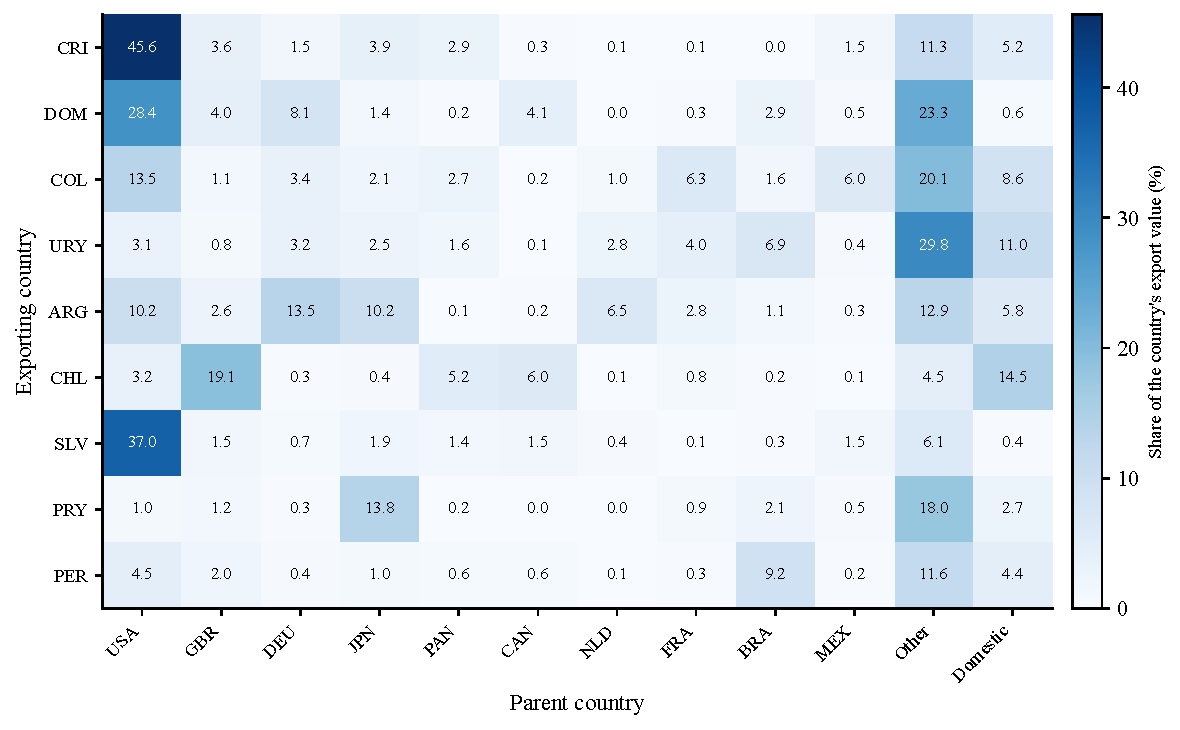
\includegraphics[width=0.9\textwidth,height=0.8\textheight,keepaspectratio]{figures/manufacturing/fig_wp1a_origin_x_parent_heatmap.pdf}%
  \caption{Manufacturing: Export Value by Exporting Country and Parent Country}%
  \label{fig:f1hm_manufacturing}%
  \par\vspace{2pt}%
  \parbox{0.92\textwidth}{\footnotesize %
  \textit{Notes:} Percent of each country's manufacturing export value, by country of the ultimate parent of the exporter.\\[3pt]%
  \textit{Source:} Authors' calculations based on customs data matched to Orbis and Dun \& Bradstreet.}%
  \end{figure}

\section{Fact 2: Foreign Multinationals Specialize in Complex Products, Domestic Multinationals in Primary Goods}\label{sec:f2_manufacturing}

\subsection{Product Complexity and Technology}
% ---- Figure: Manufacturing: Multinational Share of Export Value, by Product Complexity Quintile
\begin{figure}[H]\centering%
  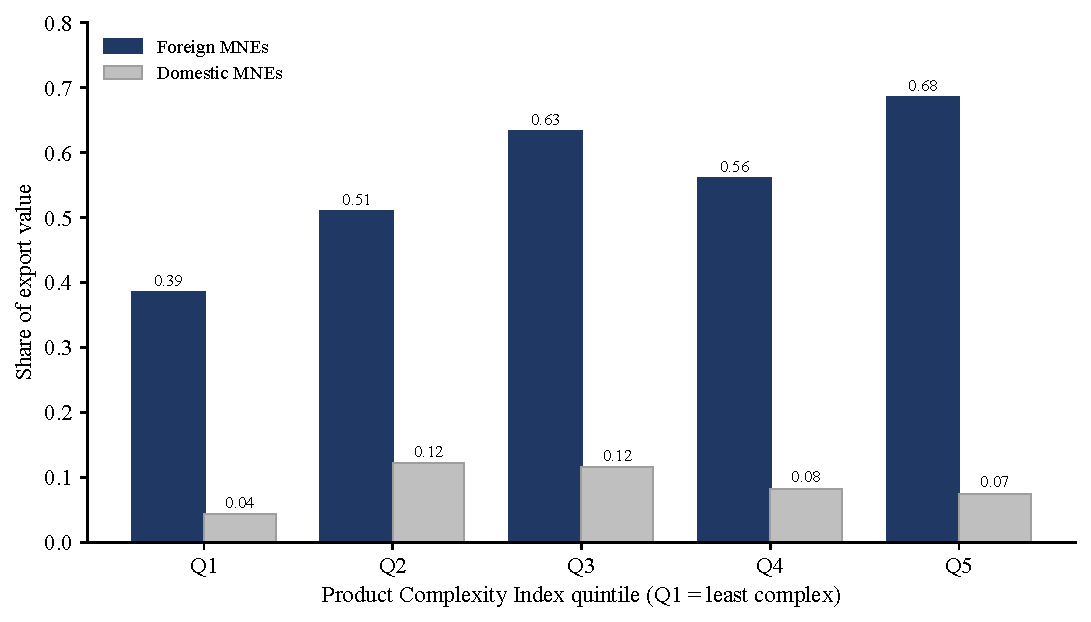
\includegraphics[width=0.78\textwidth,height=0.8\textheight,keepaspectratio]{figures/manufacturing/fig_wp0_fig2_pci.pdf}%
  \caption{Manufacturing: Multinational Share of Export Value, by Product Complexity Quintile}%
  \label{fig:pci_manufacturing}%
  \par\vspace{2pt}%
  \parbox{0.92\textwidth}{\footnotesize %
  \textit{Notes:} Shares of manufacturing export value (HS 28--97 excluding 71), all available years pooled. Quintiles of the Hausmann--Hidalgo Product Complexity Index across HS6 products (Q1 = least complex).\\[3pt]%
  \textit{Source:} Authors' calculations based on customs data matched to Orbis and Dun \& Bradstreet.}%
  \end{figure}
% ---- Figure: Manufacturing: Multinational Share of Export Value, by Technology Class
\begin{figure}[H]\centering%
  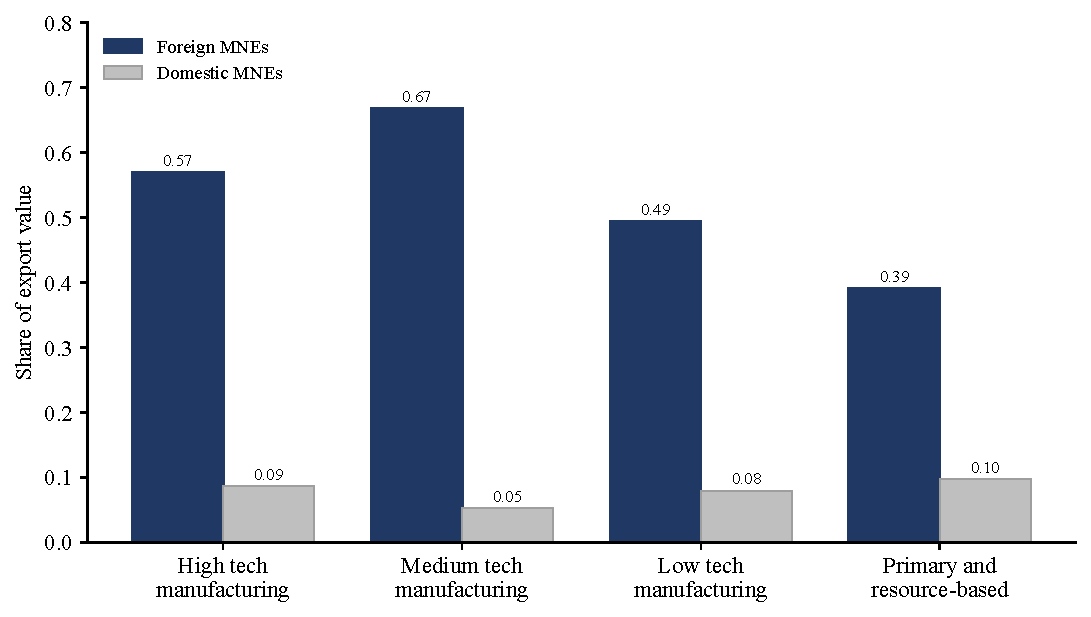
\includegraphics[width=0.78\textwidth,height=0.8\textheight,keepaspectratio]{figures/manufacturing/fig_wp0_fig3_lall.pdf}%
  \caption{Manufacturing: Multinational Share of Export Value, by Technology Class}%
  \label{fig:lall_manufacturing}%
  \par\vspace{2pt}%
  \parbox{0.92\textwidth}{\footnotesize %
  \textit{Notes:} Shares of manufacturing export value (HS 28--97 excluding 71), all available years pooled. Lall (2000) technology classes: primary and resource-based products, and low-, medium- and high-technology manufactures.\\[3pt]%
  \textit{Source:} Authors' calculations based on customs data matched to Orbis and Dun \& Bradstreet.}%
  \end{figure}

\subsection{By Parent Country}
% ---- Figure: Manufacturing: Multinational Share of Export Value, by Product Complexity Quintile and Parent Country
\begin{figure}[H]\centering%
  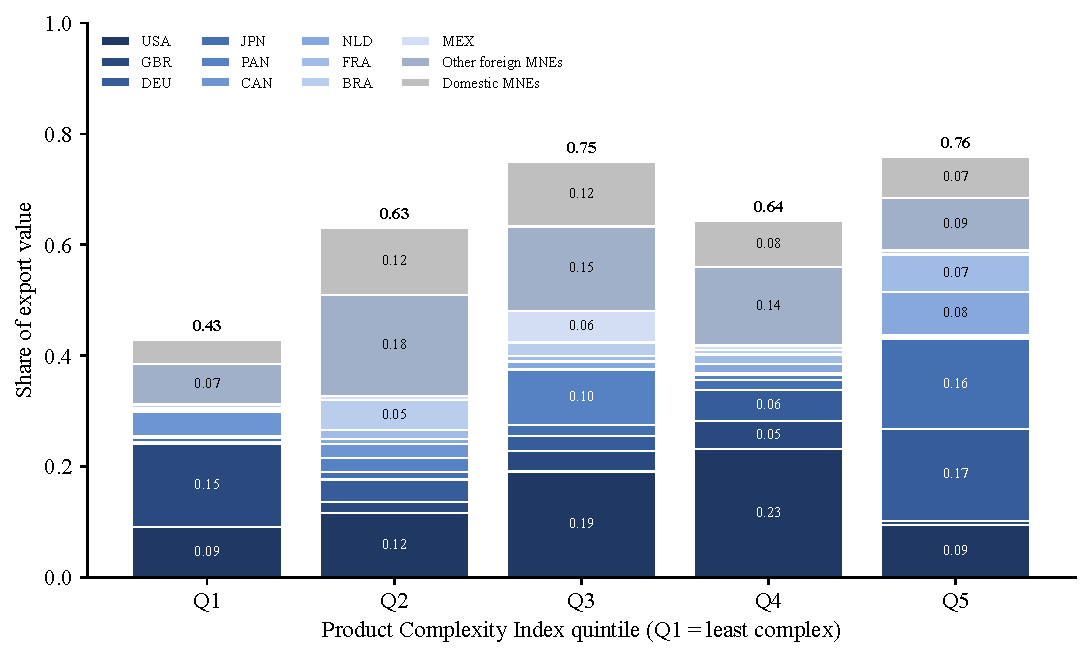
\includegraphics[width=0.92\textwidth,height=0.8\textheight,keepaspectratio]{figures/manufacturing/fig_wp1a_pci_by_parent.pdf}%
  \caption{Manufacturing: Multinational Share of Export Value, by Product Complexity Quintile and Parent Country}%
  \label{fig:pci_p_manufacturing}%
  \par\vspace{2pt}%
  \parbox{0.92\textwidth}{\footnotesize %
  \textit{Notes:} Shares of manufacturing export value (HS 28--97 excluding 71), all available years pooled. Foreign MNEs split by country of the ultimate parent. Quintiles of the Hausmann--Hidalgo Product Complexity Index across HS6 products (Q1 = least complex).\\[3pt]%
  \textit{Source:} Authors' calculations based on customs data matched to Orbis and Dun \& Bradstreet.}%
  \end{figure}
% ---- Table: Manufacturing: Multinational Share of Export Value, by Product Complexity Quintile and Parent Country
\begin{table}[H]\centering\small%
  \caption{Manufacturing: Multinational Share of Export Value, by Product Complexity Quintile and Parent Country}%
  \label{tab:pci_pn_manufacturing}%
  \adjustbox{max width=\textwidth, max totalheight=0.8\textheight}{\begin{tabular}{lcccccccccccccc}
\toprule
PCI quintile & USA & GBR & DEU & JPN & PAN & CAN & NLD & FRA & BRA & MEX & Other & Domestic & All MNEs & Value (US\$bn/yr) \\
\midrule
Q1 & 0.091 & 0.151 & 0.002 & 0.009 & 0.003 & 0.044 & 0.002 & 0.004 & 0.007 & 0.001 & 0.073 & 0.043 & 0.428 & 24.3 \\
Q2 & 0.116 & 0.020 & 0.040 & 0.014 & 0.025 & 0.025 & 0.009 & 0.016 & 0.054 & 0.008 & 0.181 & 0.122 & 0.631 & 12.7 \\
Q3 & 0.191 & 0.037 & 0.027 & 0.020 & 0.099 & 0.003 & 0.013 & 0.010 & 0.024 & 0.057 & 0.152 & 0.116 & 0.749 & 10.4 \\
Q4 & 0.232 & 0.049 & 0.057 & 0.018 & 0.008 & 0.004 & 0.017 & 0.017 & 0.008 & 0.008 & 0.142 & 0.083 & 0.643 & 11.0 \\
Q5 & 0.094 & 0.008 & 0.165 & 0.162 & 0.002 & 0.005 & 0.078 & 0.068 & 0.006 & 0.002 & 0.093 & 0.075 & 0.759 & 13.2 \\
\bottomrule
\end{tabular}
}%
  \par\vspace{3pt}%
  \begin{minipage}{0.95\textwidth}\footnotesize %
  \textit{Notes:} Shares of manufacturing export value (HS 28--97 excluding 71), all available years pooled. Other: all remaining foreign parents. Values are annual averages in US\$ billion.\\[3pt]%
  \textit{Source:} Authors' calculations based on customs data matched to Orbis and Dun \& Bradstreet.%
  \end{minipage}%
  \end{table}
% ---- Figure: Manufacturing: Multinational Share of Export Value, by Technology Class and Parent Country
\begin{figure}[H]\centering%
  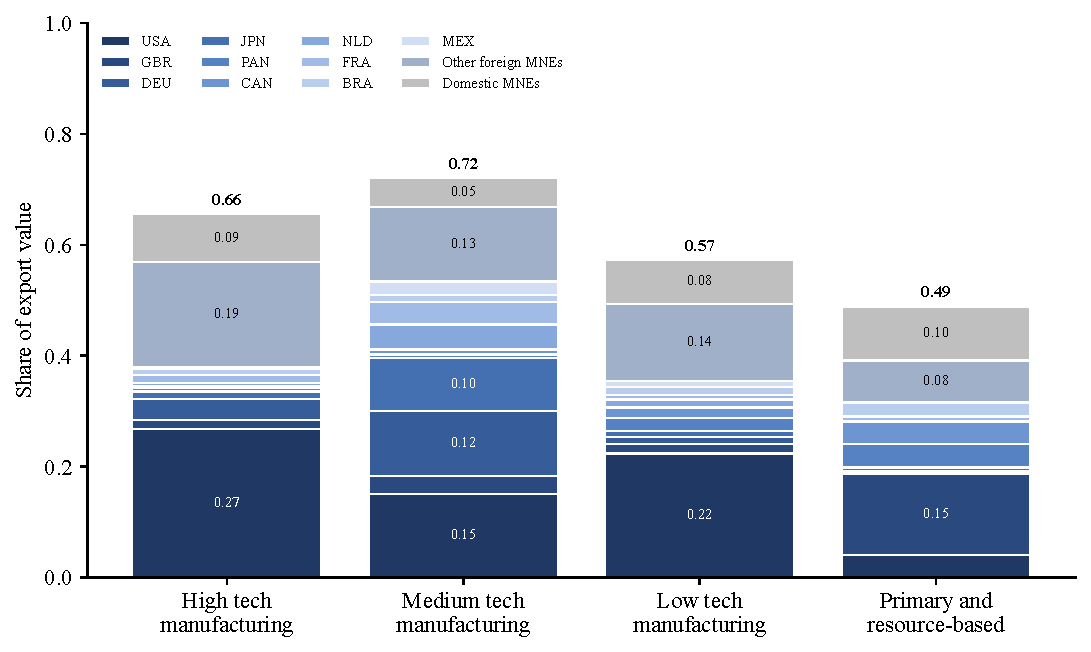
\includegraphics[width=0.92\textwidth,height=0.8\textheight,keepaspectratio]{figures/manufacturing/fig_wp1a_lall_by_parent.pdf}%
  \caption{Manufacturing: Multinational Share of Export Value, by Technology Class and Parent Country}%
  \label{fig:lall_p_manufacturing}%
  \par\vspace{2pt}%
  \parbox{0.92\textwidth}{\footnotesize %
  \textit{Notes:} Shares of manufacturing export value (HS 28--97 excluding 71), all available years pooled. Foreign MNEs split by country of the ultimate parent. Lall (2000) technology classes: primary and resource-based products, and low-, medium- and high-technology manufactures.\\[3pt]%
  \textit{Source:} Authors' calculations based on customs data matched to Orbis and Dun \& Bradstreet.}%
  \end{figure}
% ---- Table: Manufacturing: Multinational Share of Export Value, by Technology Class and Parent Country
\begin{table}[H]\centering\small%
  \caption{Manufacturing: Multinational Share of Export Value, by Technology Class and Parent Country}%
  \label{tab:lall_pn_manufacturing}%
  \adjustbox{max width=\textwidth, max totalheight=0.8\textheight}{\begin{tabular}{lcccccccccccccc}
\toprule
Technology category & USA & GBR & DEU & JPN & PAN & CAN & NLD & FRA & BRA & MEX & Other & Domestic & All MNEs & Value (US\$bn/yr) \\
\midrule
High tech manufacturing & 0.268 & 0.015 & 0.039 & 0.013 & 0.006 & 0.004 & 0.006 & 0.014 & 0.011 & 0.004 & 0.189 & 0.087 & 0.656 & 5.4 \\
Medium tech manufacturing & 0.151 & 0.033 & 0.117 & 0.095 & 0.007 & 0.009 & 0.045 & 0.040 & 0.013 & 0.025 & 0.134 & 0.053 & 0.721 & 26.5 \\
Low tech manufacturing & 0.224 & 0.017 & 0.013 & 0.011 & 0.022 & 0.019 & 0.014 & 0.008 & 0.015 & 0.010 & 0.139 & 0.079 & 0.573 & 14.7 \\
Primary and resource-based & 0.041 & 0.146 & 0.005 & 0.007 & 0.042 & 0.039 & 0.003 & 0.008 & 0.024 & 0.001 & 0.076 & 0.098 & 0.489 & 25.1 \\
\bottomrule
\end{tabular}
}%
  \par\vspace{3pt}%
  \begin{minipage}{0.95\textwidth}\footnotesize %
  \textit{Notes:} Shares of manufacturing export value (HS 28--97 excluding 71), all available years pooled. Other: all remaining foreign parents. Values are annual averages in US\$ billion.\\[3pt]%
  \textit{Source:} Authors' calculations based on customs data matched to Orbis and Dun \& Bradstreet.%
  \end{minipage}%
  \end{table}
% ---- Figure: Manufacturing: Multinational Share of Export Value, by Product Sophistication and Location of the Parent
\begin{figure}[H]\centering%
  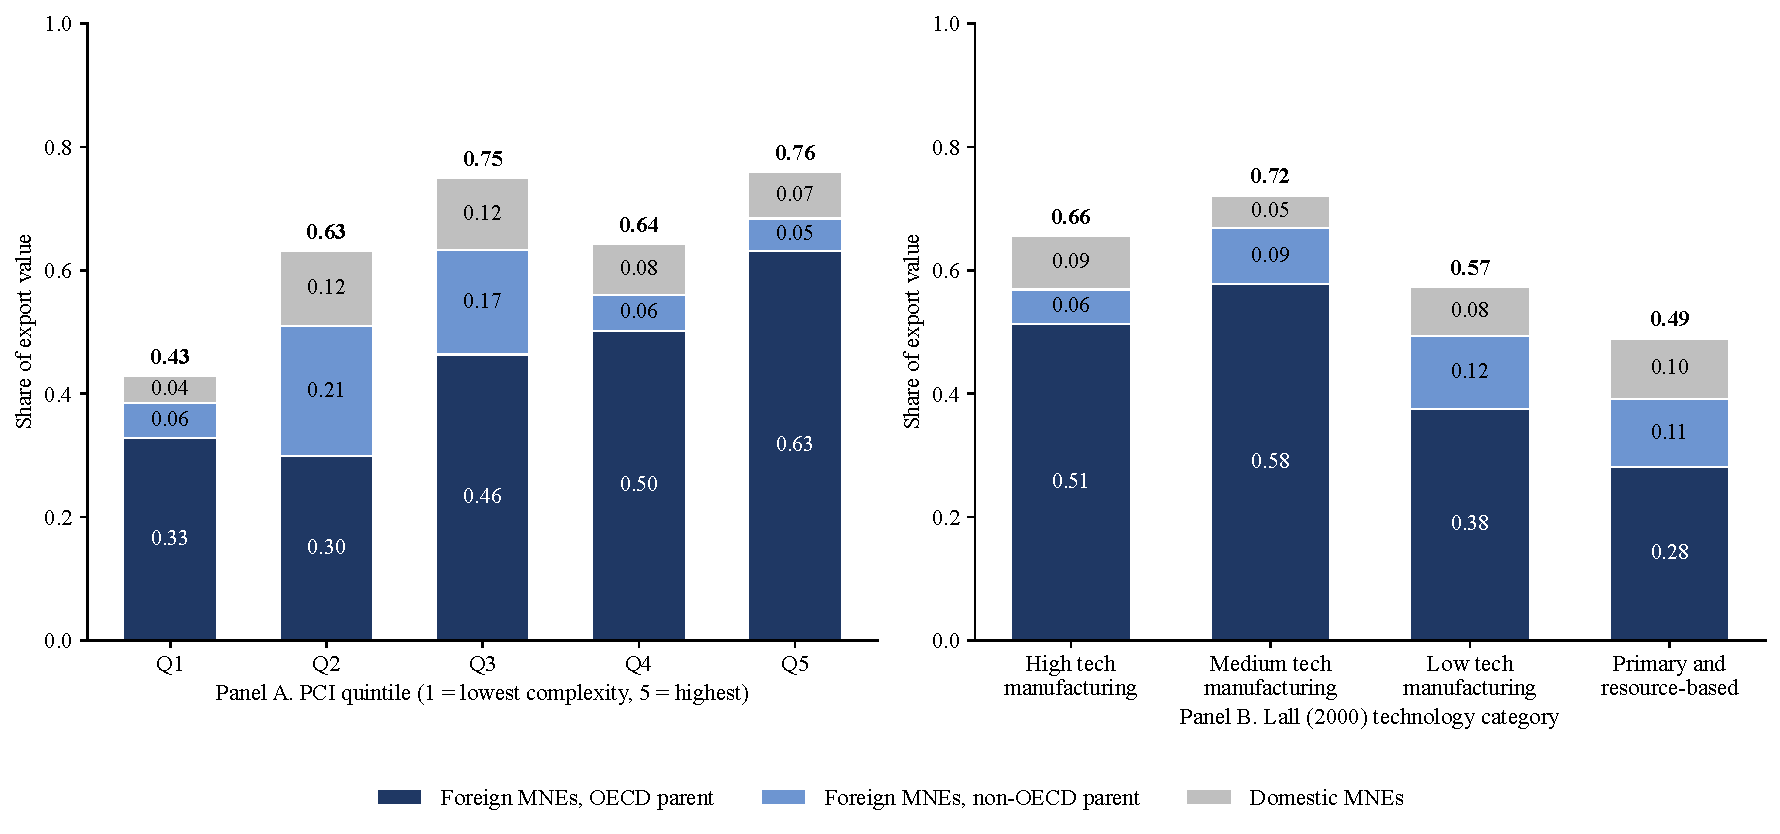
\includegraphics[width=1.0\textwidth,height=0.8\textheight,keepaspectratio]{figures/manufacturing/fig_wp1a_pci_lall_by_oecd.pdf}%
  \caption{Manufacturing: Multinational Share of Export Value, by Product Sophistication and Location of the Parent}%
  \label{fig:oecd_manufacturing}%
  \par\vspace{2pt}%
  \parbox{0.92\textwidth}{\footnotesize %
  \textit{Notes:} Shares of manufacturing export value (HS 28--97 excluding 71), all available years pooled. Foreign MNEs are split by whether the ultimate parent is in an OECD member country. Panel A: Quintiles of the Hausmann--Hidalgo Product Complexity Index across HS6 products (Q1 = least complex). Panel B: Lall (2000) technology classes: primary and resource-based products, and low-, medium- and high-technology manufactures.\\[3pt]%
  \textit{Source:} Authors' calculations based on customs data matched to Orbis and Dun \& Bradstreet.}%
  \end{figure}

\subsection{Other Measures of Product Sophistication}
% ---- Figure: Manufacturing: Multinational Share of Export Value, by Quintile of Six Sophistication Measures
\begin{figure}[H]\centering%
  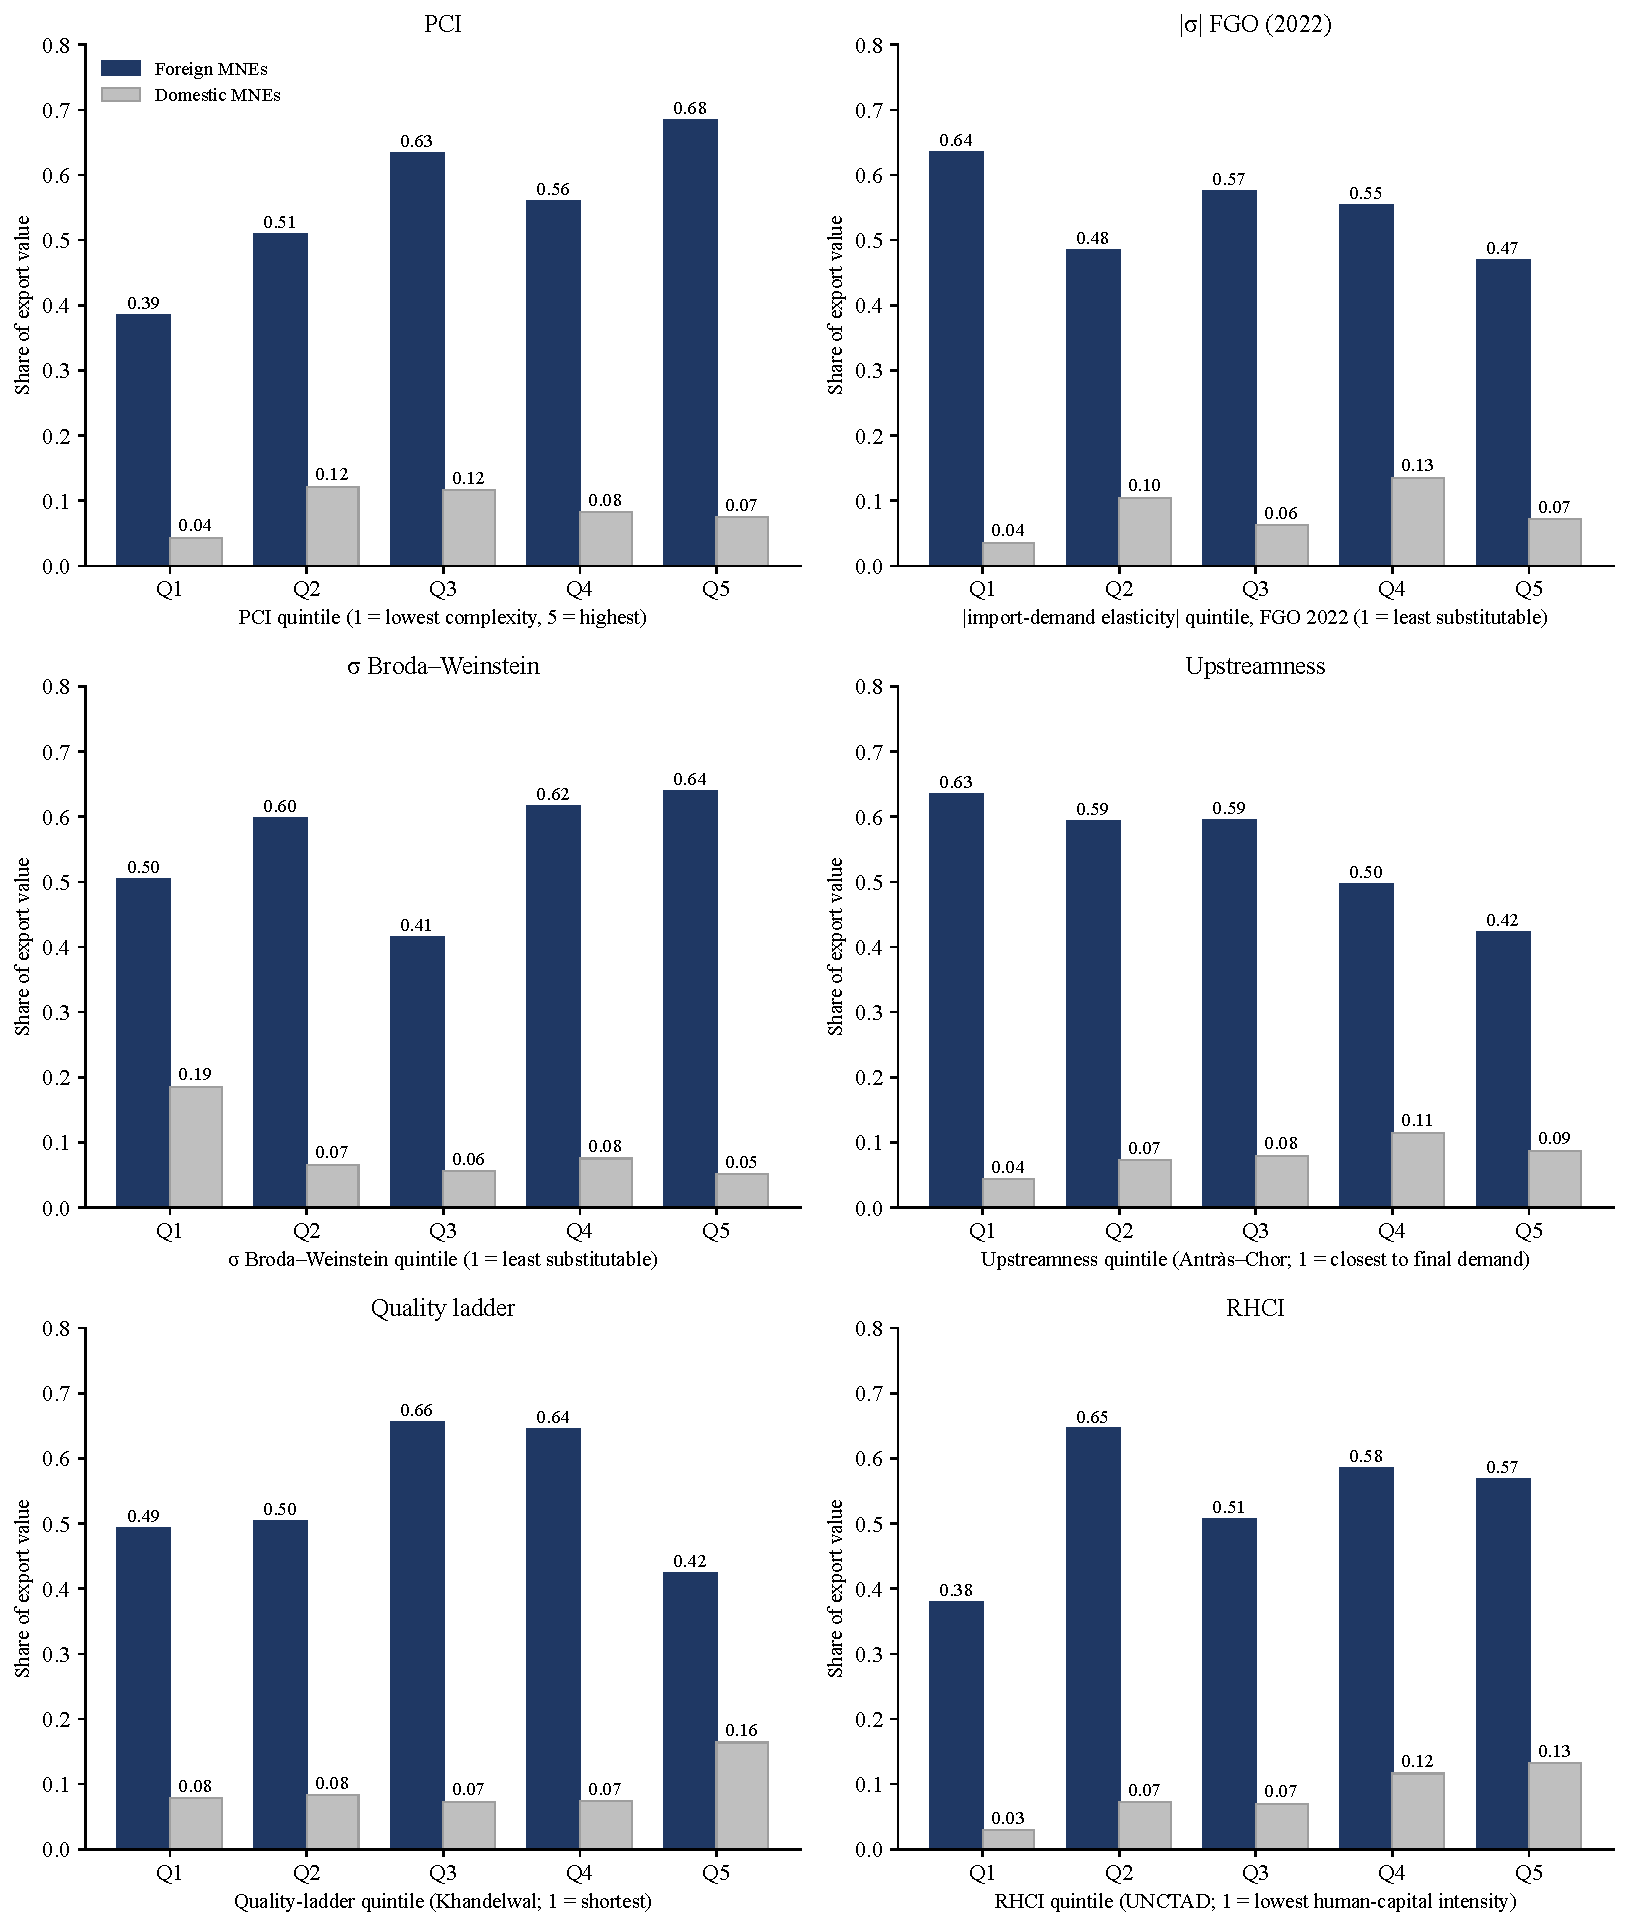
\includegraphics[width=1.0\textwidth,height=0.8\textheight,keepaspectratio]{figures/manufacturing/fig_wp1b_panel_quintiles.pdf}%
  \caption{Manufacturing: Multinational Share of Export Value, by Quintile of Six Sophistication Measures}%
  \label{fig:six_q_manufacturing}%
  \par\vspace{2pt}%
  \parbox{0.92\textwidth}{\footnotesize %
  \textit{Notes:} Shares of manufacturing export value (HS 28--97 excluding 71), all available years pooled. Quintiles computed over HS6 products. The six measures are the Product Complexity Index, the absolute import-demand elasticity of Fontagn\'e, Guimbard and Orefice (2022), the elasticity of substitution of Broda and Weinstein, upstreamness, the quality ladder and the revealed human-capital intensity of UNCTAD.\\[3pt]%
  \textit{Source:} Authors' calculations based on customs data matched to Orbis and Dun \& Bradstreet.}%
  \end{figure}
% ---- Figure: Manufacturing: Multinational Share of Export Value, by Quintile of the Import-Demand Elasticity
\begin{figure}[H]\centering%
  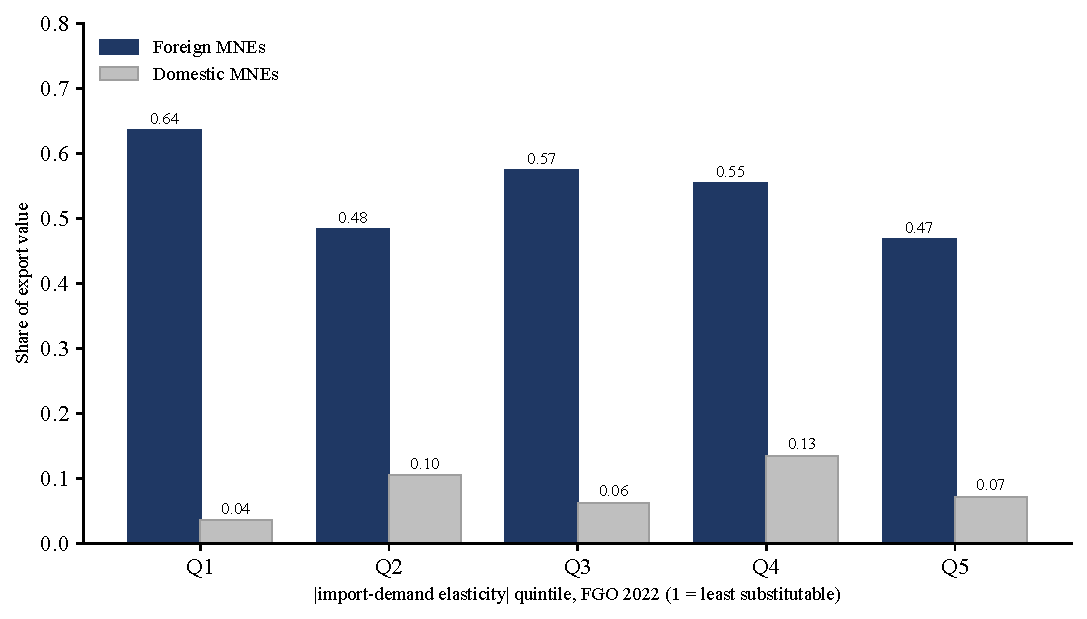
\includegraphics[width=0.78\textwidth,height=0.8\textheight,keepaspectratio]{figures/manufacturing/fig_wp1b_sigma_fgo_abs_quintile.pdf}%
  \caption{Manufacturing: Multinational Share of Export Value, by Quintile of the Import-Demand Elasticity}%
  \label{fig:fgo_q_manufacturing}%
  \par\vspace{2pt}%
  \parbox{0.92\textwidth}{\footnotesize %
  \textit{Notes:} Shares of manufacturing export value (HS 28--97 excluding 71), all available years pooled. Quintiles of the absolute import-demand elasticity of Fontagn\'e, Guimbard and Orefice (2022) across HS6 products; higher quintiles are more substitutable products.\\[3pt]%
  \textit{Source:} Authors' calculations based on customs data matched to Orbis and Dun \& Bradstreet.}%
  \end{figure}
% ---- Figure: Manufacturing: Distribution of Export Value across Six Sophistication Measures
\begin{figure}[H]\centering%
  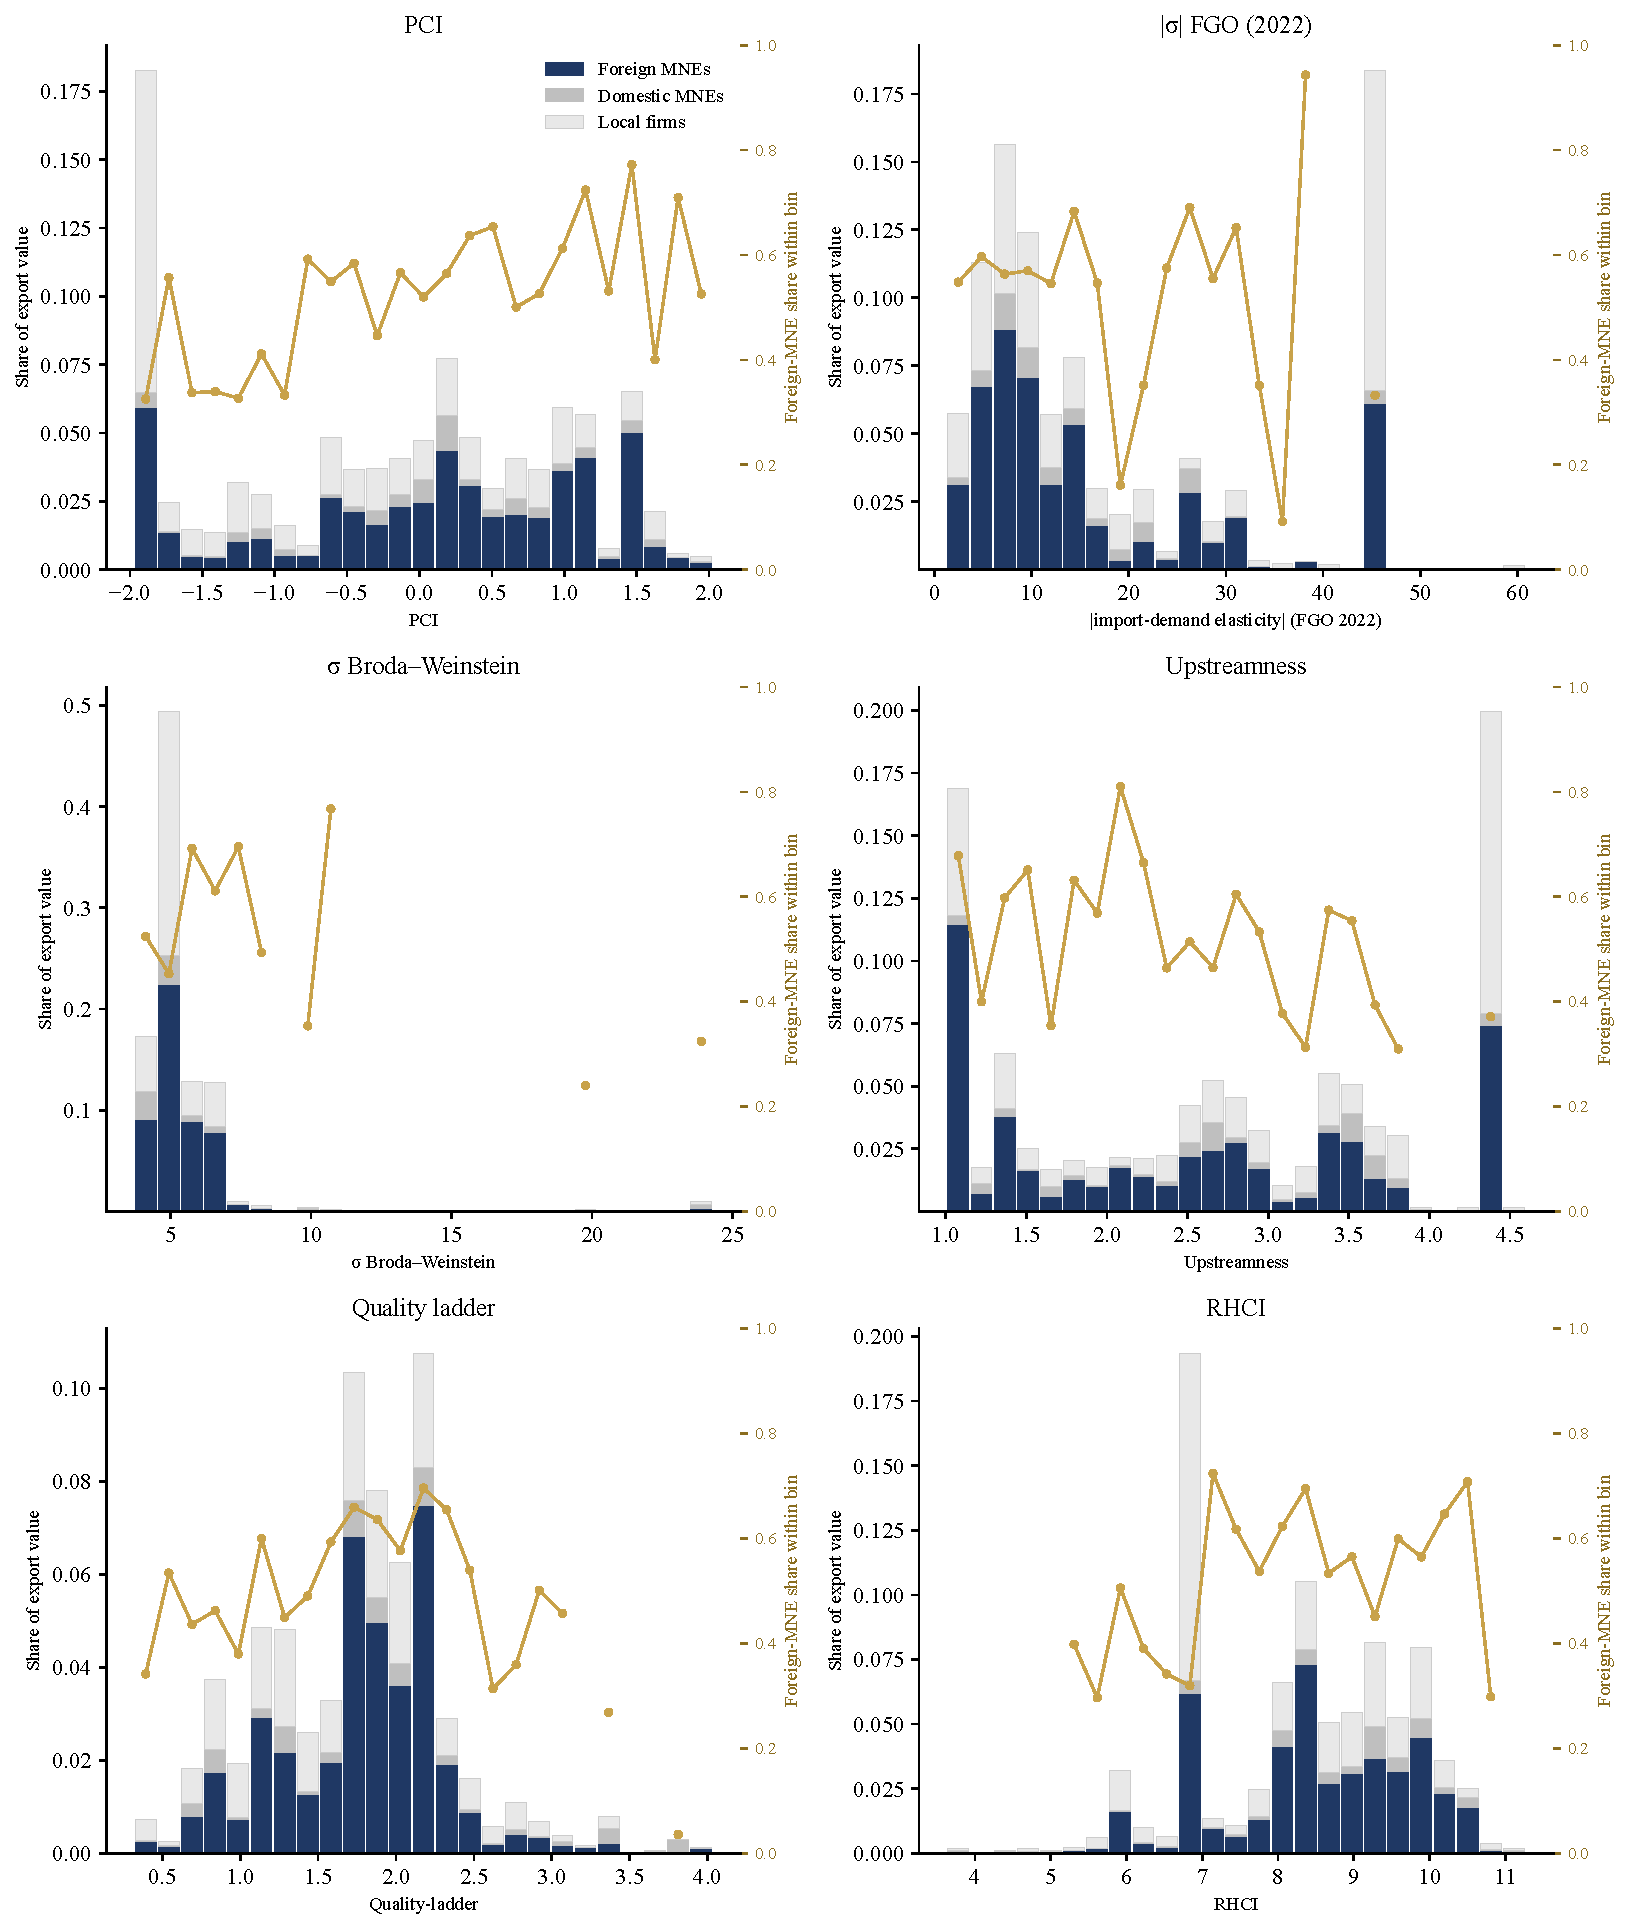
\includegraphics[width=1.0\textwidth,height=0.8\textheight,keepaspectratio]{figures/manufacturing/fig_wp1b_panel_hist.pdf}%
  \caption{Manufacturing: Distribution of Export Value across Six Sophistication Measures}%
  \label{fig:six_h_manufacturing}%
  \par\vspace{2pt}%
  \parbox{0.92\textwidth}{\footnotesize %
  \textit{Notes:} Bars: manufacturing export value (HS 28--97 excluding 71) in each bin, by type of exporter. Line (right axis): foreign-MNE share of each bin. The six measures are the Product Complexity Index, the absolute import-demand elasticity of Fontagn\'e, Guimbard and Orefice (2022), the elasticity of substitution of Broda and Weinstein, upstreamness, the quality ladder and the revealed human-capital intensity of UNCTAD.\\[3pt]%
  \textit{Source:} Authors' calculations based on customs data matched to Orbis and Dun \& Bradstreet.}%
  \end{figure}
% ---- Figure: Manufacturing: Distribution of Export Value across the Import-Demand Elasticity
\begin{figure}[H]\centering%
  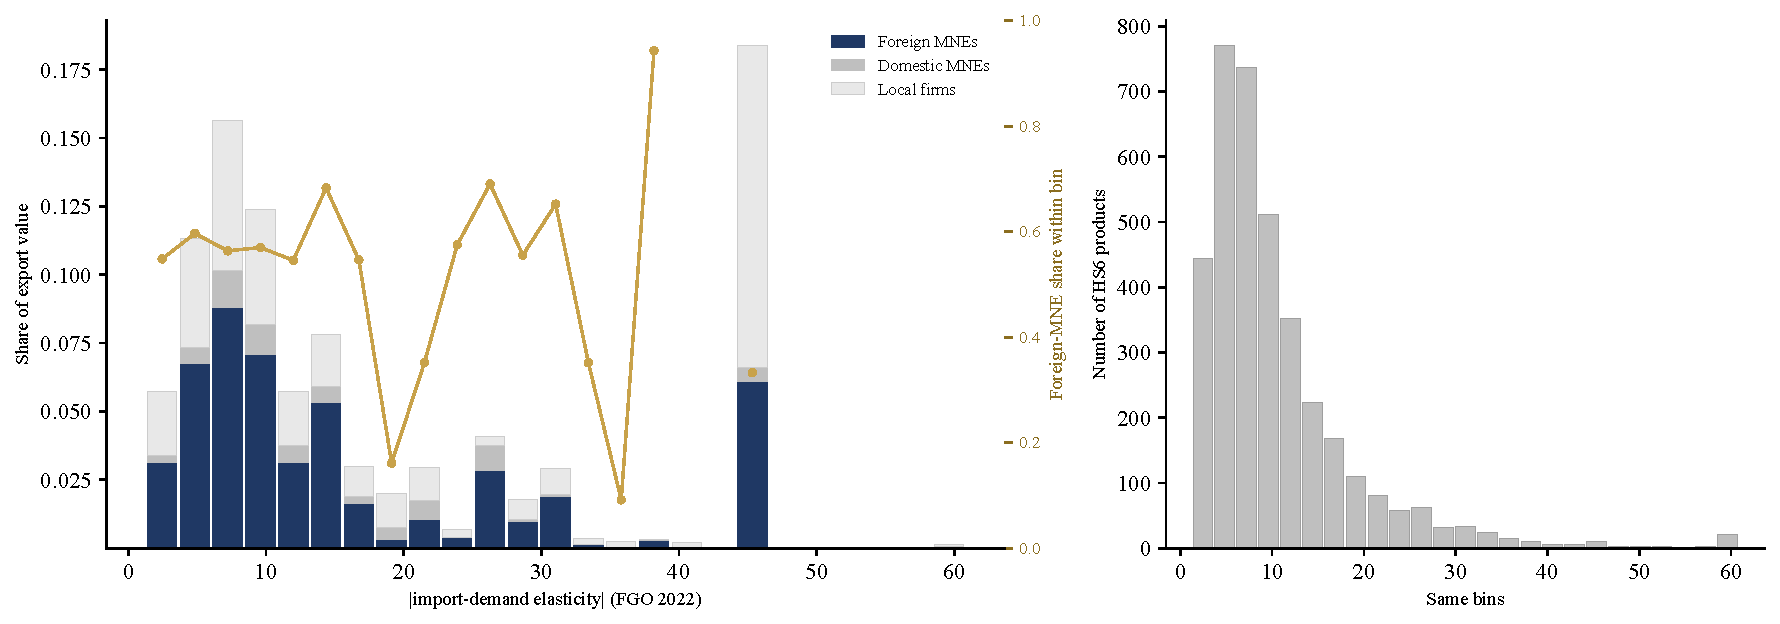
\includegraphics[width=1.0\textwidth,height=0.8\textheight,keepaspectratio]{figures/manufacturing/fig_wp1b_hist_sigma_fgo_abs.pdf}%
  \caption{Manufacturing: Distribution of Export Value across the Import-Demand Elasticity}%
  \label{fig:fgo_h_manufacturing}%
  \par\vspace{2pt}%
  \parbox{0.92\textwidth}{\footnotesize %
  \textit{Notes:} Left: export value in each bin, by type of exporter, and the foreign-MNE share of each bin. Right: number of HS6 products in each bin.\\[3pt]%
  \textit{Source:} Authors' calculations based on customs data matched to Orbis and Dun \& Bradstreet.}%
  \end{figure}
% ---- Figure: Manufacturing: Distribution of Export Value across the Product Complexity Index
\begin{figure}[H]\centering%
  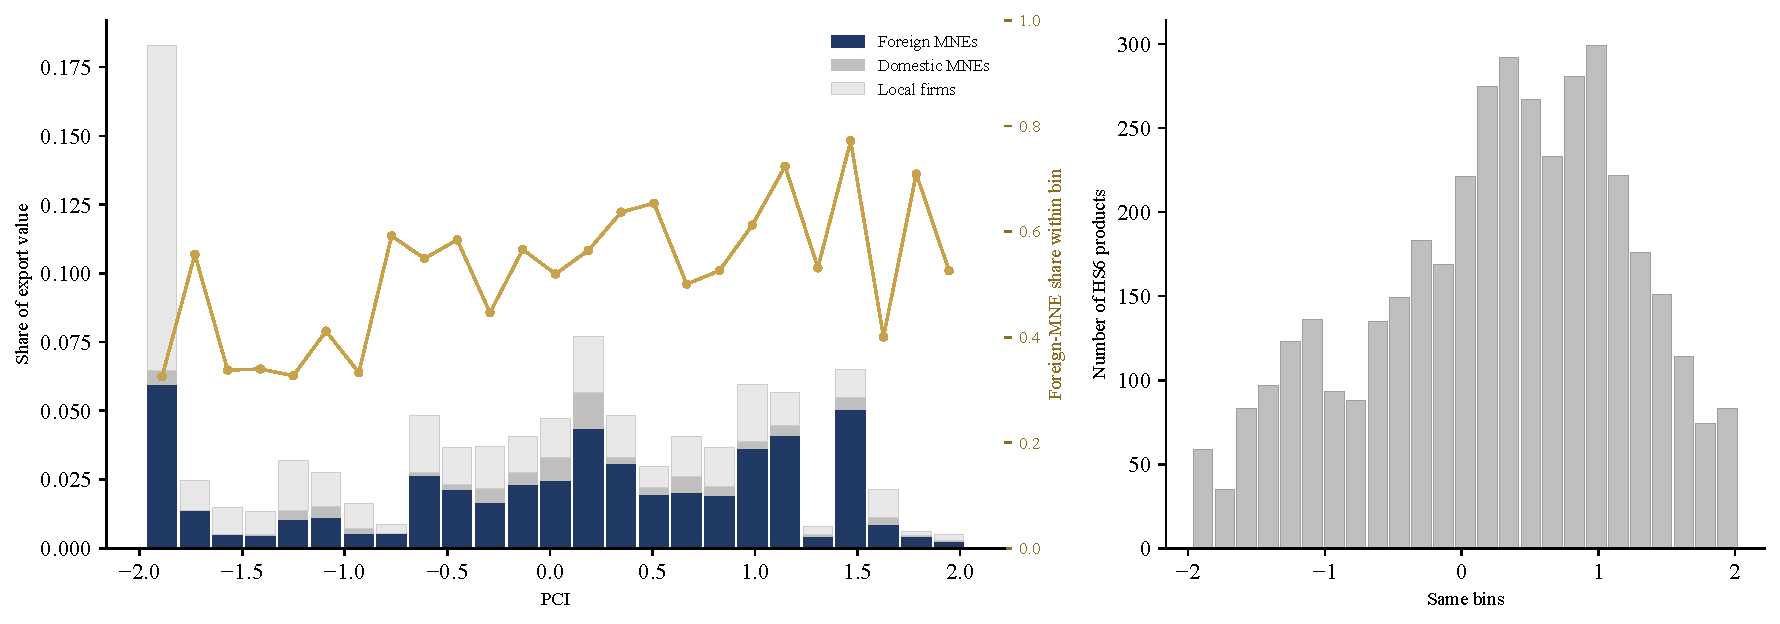
\includegraphics[width=1.0\textwidth,height=0.8\textheight,keepaspectratio]{figures/manufacturing/fig_wp1b_hist_complexity.pdf}%
  \caption{Manufacturing: Distribution of Export Value across the Product Complexity Index}%
  \label{fig:pci_h_manufacturing}%
  \par\vspace{2pt}%
  \parbox{0.92\textwidth}{\footnotesize %
  \textit{Notes:} Left: export value in each bin, by type of exporter, and the foreign-MNE share of each bin. Right: number of HS6 products in each bin.\\[3pt]%
  \textit{Source:} Authors' calculations based on customs data matched to Orbis and Dun \& Bradstreet.}%
  \end{figure}
% ---- Table: Manufacturing: Multinational Share of Export Value, by Quintile of Six Sophistication Measures
\begin{table}[H]\centering\small%
  \caption{Manufacturing: Multinational Share of Export Value, by Quintile of Six Sophistication Measures}%
  \label{tab:six_t_manufacturing}%
  \adjustbox{max width=\textwidth, max totalheight=0.8\textheight}{\begin{tabular}{lccccc|ccccc}
\toprule
 & \multicolumn{5}{c}{Foreign MNE share} & \multicolumn{5}{c}{Domestic MNE share} \\
Measure & Q1 & Q2 & Q3 & Q4 & Q5 & Q1 & Q2 & Q3 & Q4 & Q5 \\
\midrule
PCI & 0.39 & 0.51 & 0.63 & 0.56 & 0.68 & 0.04 & 0.12 & 0.12 & 0.08 & 0.07 \\
$|\sigma|$ FGO (2022) & 0.64 & 0.48 & 0.57 & 0.55 & 0.47 & 0.04 & 0.10 & 0.06 & 0.13 & 0.07 \\
$\sigma$ Broda--Weinstein & 0.50 & 0.60 & 0.41 & 0.62 & 0.64 & 0.19 & 0.07 & 0.06 & 0.08 & 0.05 \\
Upstreamness & 0.63 & 0.59 & 0.59 & 0.50 & 0.42 & 0.04 & 0.07 & 0.08 & 0.11 & 0.09 \\
Quality ladder & 0.49 & 0.50 & 0.66 & 0.64 & 0.42 & 0.08 & 0.08 & 0.07 & 0.07 & 0.16 \\
RHCI & 0.38 & 0.65 & 0.51 & 0.58 & 0.57 & 0.03 & 0.07 & 0.07 & 0.12 & 0.13 \\
\bottomrule
\end{tabular}
}%
  \par\vspace{3pt}%
  \begin{minipage}{0.95\textwidth}\footnotesize %
  \textit{Notes:} Shares of manufacturing export value (HS 28--97 excluding 71), all available years pooled. Quintiles computed over HS6 products. --: fewer than 30 HS6 products carry the measure.\\[3pt]%
  \textit{Source:} Authors' calculations based on customs data matched to Orbis and Dun \& Bradstreet.%
  \end{minipage}%
  \end{table}
% ---- Table: Manufacturing: Correlations between Sophistication Measures
\begin{table}[H]\centering\small%
  \caption{Manufacturing: Correlations between Sophistication Measures}%
  \label{tab:corr_manufacturing}%
  \adjustbox{max width=\textwidth, max totalheight=0.8\textheight}{\begin{tabular}{lrrrrrr}
\toprule
 & PCI & $|\sigma|$ FGO (2022) & $\sigma$ Broda--Weinstein & Upstreamness & Quality ladder & RHCI \\
\midrule
PCI & 1.00 & -0.61 & 0.06 & -0.52 & 0.29 & 0.79 \\
$|\sigma|$ FGO (2022) & -0.61 & 1.00 & -0.05 & 0.74 & 0.12 & -0.43 \\
$\sigma$ Broda--Weinstein & 0.06 & -0.05 & 1.00 & -0.15 & -0.12 & 0.08 \\
Upstreamness & -0.52 & 0.74 & -0.15 & 1.00 & 0.13 & -0.32 \\
Quality ladder & 0.29 & 0.12 & -0.12 & 0.13 & 1.00 & 0.36 \\
RHCI & 0.79 & -0.43 & 0.08 & -0.32 & 0.36 & 1.00 \\
\bottomrule
\end{tabular}
}%
  \par\vspace{3pt}%
  \begin{minipage}{0.95\textwidth}\footnotesize %
  \textit{Notes:} Correlations across HS6 products, weighted by export value.\\[3pt]%
  \textit{Source:} Authors' calculations based on customs data matched to Orbis and Dun \& Bradstreet.%
  \end{minipage}%
  \end{table}

\subsection{Rauch Classes and End Use}
% ---- Table: Manufacturing: Multinational Share of Export Value, by Rauch Product Class
\begin{table}[H]\centering\small%
  \caption{Manufacturing: Multinational Share of Export Value, by Rauch Product Class}%
  \label{tab:rauch_manufacturing}%
  \adjustbox{max width=\textwidth, max totalheight=0.8\textheight}{\begin{tabular}{lcccrr}
\toprule
Rauch (1999) class & Foreign & Domestic & All MNEs & HS6 products & Value (US\$bn/yr) \\
\midrule
Differentiated & 0.599 & 0.049 & 0.649 & 2,505 & 36.2 \\
Reference-priced & 0.495 & 0.165 & 0.661 & 1,180 & 18.6 \\
Homogeneous (exchange) & 0.368 & 0.025 & 0.393 & 128 & 14.4 \\
\bottomrule
\end{tabular}
}%
  \par\vspace{3pt}%
  \begin{minipage}{0.95\textwidth}\footnotesize %
  \textit{Notes:} Shares of manufacturing export value (HS 28--97 excluding 71), all available years pooled. Rauch (1999) conservative classification: homogeneous goods are traded on organized exchanges, reference-priced goods have a price quoted in trade publications, and differentiated goods have neither. Values are annual averages in US\$ billion.\\[3pt]%
  \textit{Source:} Authors' calculations based on customs data matched to Orbis and Dun \& Bradstreet.%
  \end{minipage}%
  \end{table}
% ---- Figure: Manufacturing: Multinational Share of Export Value, by Rauch Product Class
\begin{figure}[H]\centering%
  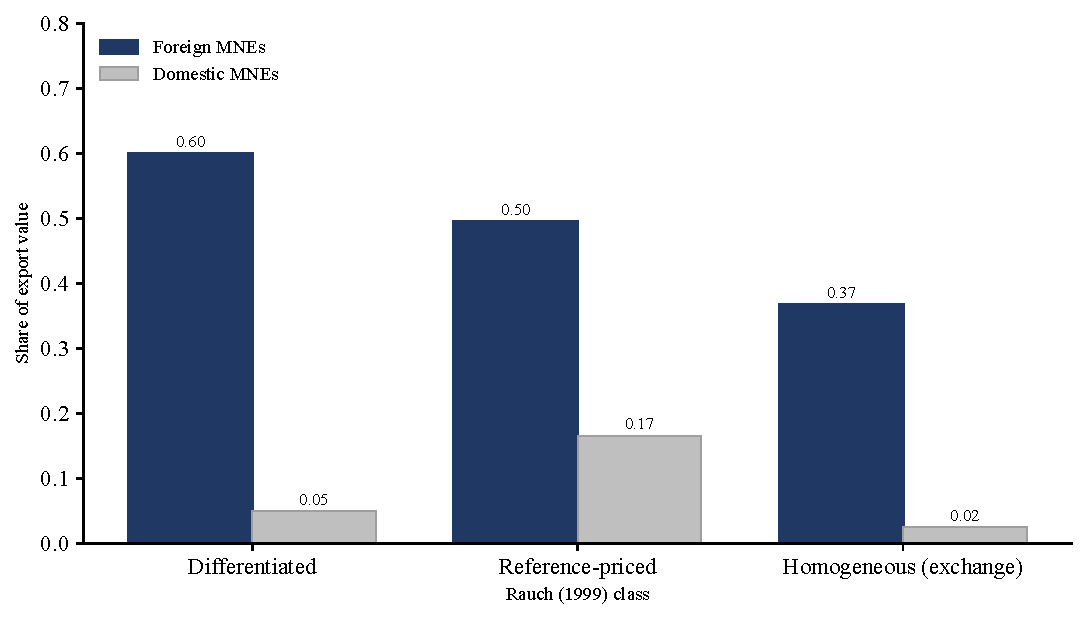
\includegraphics[width=0.7\textwidth,height=0.8\textheight,keepaspectratio]{figures/manufacturing/fig_wp1b_rauch.pdf}%
  \caption{Manufacturing: Multinational Share of Export Value, by Rauch Product Class}%
  \label{fig:rauch_f_manufacturing}%
  \par\vspace{2pt}%
  \parbox{0.92\textwidth}{\footnotesize %
  \textit{Notes:} Shares of manufacturing export value (HS 28--97 excluding 71), all available years pooled. Rauch (1999) conservative classification: homogeneous goods are traded on organized exchanges, reference-priced goods have a price quoted in trade publications, and differentiated goods have neither.\\[3pt]%
  \textit{Source:} Authors' calculations based on customs data matched to Orbis and Dun \& Bradstreet.}%
  \end{figure}
% ---- Table: Manufacturing: Multinational Share of Export Value: Differentiated and Other Products
\begin{table}[H]\centering\small%
  \caption{Manufacturing: Multinational Share of Export Value: Differentiated and Other Products}%
  \label{tab:rauch2_manufacturing}%
  \adjustbox{max width=\textwidth, max totalheight=0.8\textheight}{\begin{tabular}{lcccrr}
\toprule
Rauch (1999): differentiated vs non-differentiated & Foreign & Domestic & All MNEs & HS6 products & Value (US\$bn/yr) \\
\midrule
Differentiated & 0.599 & 0.049 & 0.649 & 2,505 & 36.2 \\
Non-differentiated & 0.435 & 0.099 & 0.534 & 1,308 & 33.0 \\
\bottomrule
\end{tabular}
}%
  \par\vspace{3pt}%
  \begin{minipage}{0.95\textwidth}\footnotesize %
  \textit{Notes:} Shares of manufacturing export value (HS 28--97 excluding 71), all available years pooled. Rauch (1999) conservative classification; other products are reference-priced and homogeneous goods. Values are annual averages in US\$ billion.\\[3pt]%
  \textit{Source:} Authors' calculations based on customs data matched to Orbis and Dun \& Bradstreet.%
  \end{minipage}%
  \end{table}
% ---- Figure: Manufacturing: Multinational Share of Export Value: Differentiated and Other Products
\begin{figure}[H]\centering%
  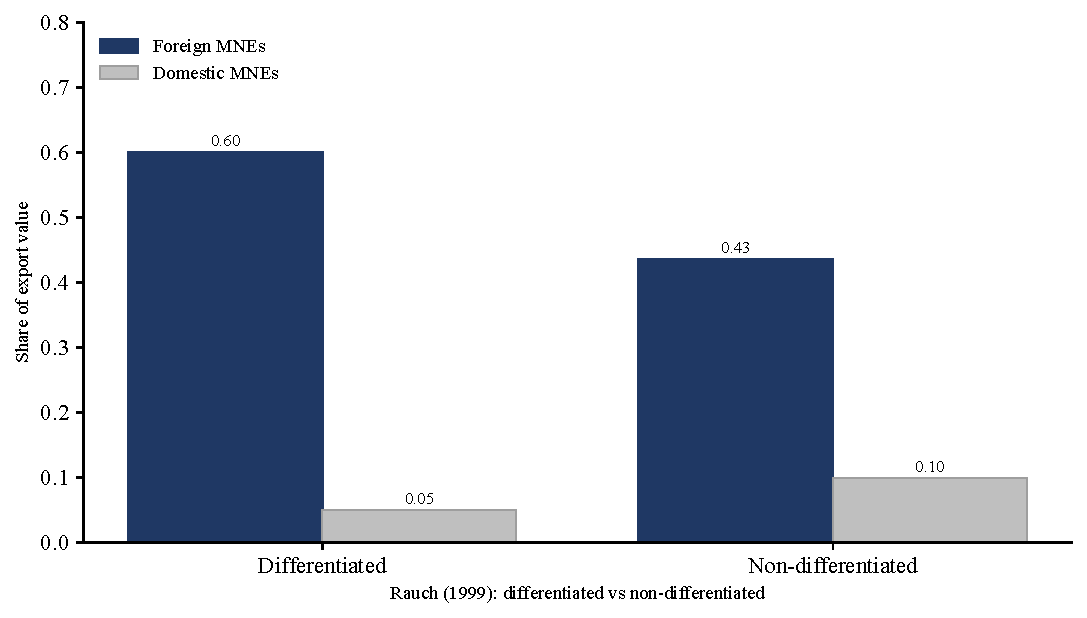
\includegraphics[width=0.7\textwidth,height=0.8\textheight,keepaspectratio]{figures/manufacturing/fig_wp1b_rauch2.pdf}%
  \caption{Manufacturing: Multinational Share of Export Value: Differentiated and Other Products}%
  \label{fig:rauch2_f_manufacturing}%
  \par\vspace{2pt}%
  \parbox{0.92\textwidth}{\footnotesize %
  \textit{Notes:} Shares of manufacturing export value (HS 28--97 excluding 71), all available years pooled. Rauch (1999) conservative classification; other products are reference-priced and homogeneous goods.\\[3pt]%
  \textit{Source:} Authors' calculations based on customs data matched to Orbis and Dun \& Bradstreet.}%
  \end{figure}
% ---- Table: Manufacturing: Multinational Share of Export Value, by End Use
\begin{table}[H]\centering\small%
  \caption{Manufacturing: Multinational Share of Export Value, by End Use}%
  \label{tab:bec_manufacturing}%
  \adjustbox{max width=\textwidth, max totalheight=0.8\textheight}{\begin{tabular}{lcccrr}
\toprule
BEC end use & Foreign & Domestic & All MNEs & HS6 products & Value (US\$bn/yr) \\
\midrule
Intermediate & 0.469 & 0.091 & 0.560 & 2,668 & 47.2 \\
Consumption & 0.606 & 0.049 & 0.655 & 734 & 15.2 \\
Capital & 0.648 & 0.056 & 0.704 & 654 & 9.3 \\
\bottomrule
\end{tabular}
}%
  \par\vspace{3pt}%
  \begin{minipage}{0.95\textwidth}\footnotesize %
  \textit{Notes:} Shares of manufacturing export value (HS 28--97 excluding 71), all available years pooled. End use from BEC Rev.\,4; HS6 products without a BEC correspondence are excluded. Values are annual averages in US\$ billion.\\[3pt]%
  \textit{Source:} Authors' calculations based on customs data matched to Orbis and Dun \& Bradstreet.%
  \end{minipage}%
  \end{table}

\subsection{Regressions}
% ---- Table: Manufacturing: Product Characteristics and Multinational Shares
\begin{table}[H]\centering\small%
  \caption{Manufacturing: Product Characteristics and Multinational Shares}%
  \label{tab:fgo_r_manufacturing}%
  \adjustbox{max width=\textwidth, max totalheight=0.8\textheight}{\begin{tabular}{lccc} \hline
 & (1) & (2) & (3) \\ \hline
\multicolumn{4}{l}{\textit{Panel A. Dependent variable: share of all MNEs}} \\
Complexity (PCI) & 0.0873*** & 0.0859*** & 0.0825*** \\
 & (0.0038) & (0.0037) & (0.0038) \\
$|\sigma|$ FGO (per s.d.) & -0.0153*** & -0.0169*** & -0.0200*** \\
 & (0.0022) & (0.0021) & (0.0021) \\
Upstreamness & -0.0330*** & -0.0328*** & -0.0216*** \\
 & (0.0043) & (0.0041) & (0.0042) \\
\midrule
\multicolumn{4}{l}{\textit{Panel B. Dependent variable: share of foreign MNEs}} \\
Complexity (PCI) & 0.0607*** & 0.0604*** & 0.0602*** \\
 & (0.0043) & (0.0041) & (0.0041) \\
$|\sigma|$ FGO (per s.d.) & 0.0092*** & 0.0065*** & 0.0033 \\
 & (0.0026) & (0.0024) & (0.0024) \\
Upstreamness & -0.0434*** & -0.0435*** & -0.0267*** \\
 & (0.0045) & (0.0043) & (0.0041) \\
\midrule
\multicolumn{4}{l}{\textit{Panel C. Dependent variable: share of domestic MNEs}} \\
Complexity (PCI) & 0.0266*** & 0.0255*** & 0.0222*** \\
 & (0.0031) & (0.0028) & (0.0029) \\
$|\sigma|$ FGO (per s.d.) & -0.0245*** & -0.0235*** & -0.0233*** \\
 & (0.0020) & (0.0018) & (0.0021) \\
Upstreamness & 0.0104*** & 0.0107*** & 0.0052* \\
 & (0.0023) & (0.0024) & (0.0030) \\
\hline
Origin FE & $\checkmark$ &  &  \\
Destination FE & $\checkmark$ &  &  \\
Year FE & $\checkmark$ &  &  \\
Origin $\times$ year FE &  & $\checkmark$ &  \\
Destination $\times$ year FE &  & $\checkmark$ &  \\
Origin $\times$ dest.\ $\times$ year FE &  &  & $\checkmark$ \\
Observations & 1,388,296 & 1,388,073 & 1,386,580 \\
\hline
\end{tabular}
}%
  \par\vspace{3pt}%
  \begin{minipage}{0.95\textwidth}\footnotesize %
  \textit{Notes:} Observations are origin--destination--HS6--year cells. Manufacturing products only. Dependent variable: share of the cell's export value shipped by each type of MNE. The import-demand elasticity is standardized (mean 0, standard deviation 1). Regressions weighted by the cell's export value. Robust standard errors in parentheses. *** $p<0.01$, ** $p<0.05$, * $p<0.1$.\\[3pt]%
  \textit{Source:} Authors' calculations based on customs data matched to Orbis and Dun \& Bradstreet.%
  \end{minipage}%
  \end{table}
% ---- Table: Manufacturing: Product Sophistication and Multinational Shares
\begin{table}[H]\centering\footnotesize%
  \caption{Manufacturing: Product Sophistication and Multinational Shares}%
  \label{tab:meas_r_manufacturing}%
  \adjustbox{max width=\textwidth, max totalheight=0.8\textheight}{\begin{tabular}{lcccccc} \hline
 & \multicolumn{2}{c}{PCI} & \multicolumn{2}{c}{Lall} & \multicolumn{2}{c}{Rauch} \\
 & (1) & (2) & (3) & (4) & (5) & (6) \\ \hline
\multicolumn{7}{l}{\textit{Panel A. Dependent variable: share of all MNEs}} \\
Complexity (PCI) & 0.1107*** & 0.1062*** &  &  &  &  \\
 & (0.0041) & (0.0040) &  &  &  &  \\
Lall: high tech (vs primary and resource-based) &  &  & 0.0969*** & 0.0729*** &  &  \\
 &  &  & (0.0142) & (0.0152) &  &  \\
Lall: medium tech &  &  & 0.1720*** & 0.1443*** &  &  \\
 &  &  & (0.0099) & (0.0090) &  &  \\
Lall: low tech &  &  & 0.0799*** & 0.0562*** &  &  \\
 &  &  & (0.0091) & (0.0085) &  &  \\
Rauch: differentiated (vs homogeneous) &  &  &  &  & 0.2448*** & 0.2232*** \\
 &  &  &  &  & (0.0136) & (0.0131) \\
Rauch: reference-priced &  &  &  &  & 0.2642*** & 0.2662*** \\
 &  &  &  &  & (0.0133) & (0.0135) \\
Observations & 1,480,362 & 1,478,870 & 1,481,180 & 1,479,691 & 1,370,899 & 1,369,380 \\
\midrule
\multicolumn{7}{l}{\textit{Panel B. Dependent variable: share of foreign MNEs}} \\
Complexity (PCI) & 0.0696*** & 0.0676*** &  &  &  &  \\
 & (0.0046) & (0.0044) &  &  &  &  \\
Lall: high tech (vs primary and resource-based) &  &  & 0.0603*** & 0.0389*** &  &  \\
 &  &  & (0.0145) & (0.0134) &  &  \\
Lall: medium tech &  &  & 0.1797*** & 0.1558*** &  &  \\
 &  &  & (0.0097) & (0.0087) &  &  \\
Lall: low tech &  &  & 0.0336*** & 0.0162* &  &  \\
 &  &  & (0.0093) & (0.0087) &  &  \\
Rauch: differentiated (vs homogeneous) &  &  &  &  & 0.0980*** & 0.0738*** \\
 &  &  &  &  & (0.0162) & (0.0160) \\
Rauch: reference-priced &  &  &  &  & 0.0518*** & 0.0494*** \\
 &  &  &  &  & (0.0162) & (0.0168) \\
Observations & 1,480,362 & 1,478,870 & 1,481,180 & 1,479,691 & 1,370,899 & 1,369,380 \\
\midrule
\multicolumn{7}{l}{\textit{Panel C. Dependent variable: share of domestic MNEs}} \\
Complexity (PCI) & 0.0411*** & 0.0386*** &  &  &  &  \\
 & (0.0036) & (0.0039) &  &  &  &  \\
Lall: high tech (vs primary and resource-based) &  &  & 0.0366*** & 0.0340*** &  &  \\
 &  &  & (0.0138) & (0.0128) &  &  \\
Lall: medium tech &  &  & -0.0078* & -0.0115*** &  &  \\
 &  &  & (0.0043) & (0.0045) &  &  \\
Lall: low tech &  &  & 0.0463*** & 0.0400*** &  &  \\
 &  &  & (0.0057) & (0.0054) &  &  \\
Rauch: differentiated (vs homogeneous) &  &  &  &  & 0.1468*** & 0.1494*** \\
 &  &  &  &  & (0.0109) & (0.0128) \\
Rauch: reference-priced &  &  &  &  & 0.2125*** & 0.2168*** \\
 &  &  &  &  & (0.0131) & (0.0153) \\
Observations & 1,480,362 & 1,478,870 & 1,481,180 & 1,479,691 & 1,370,899 & 1,369,380 \\
\hline
Origin $\times$ year and destination $\times$ year FE & $\checkmark$ &  & $\checkmark$ &  & $\checkmark$ &  \\
Origin $\times$ dest.\ $\times$ year FE &  & $\checkmark$ &  & $\checkmark$ &  & $\checkmark$ \\
\hline
\end{tabular}
}%
  \par\vspace{3pt}%
  \begin{minipage}{0.95\textwidth}\footnotesize %
  \textit{Notes:} Observations are origin--destination--HS6--year cells. Manufacturing products only. Dependent variable: share of the cell's export value shipped by each type of MNE. Omitted categories: primary and resource-based products (Lall) and homogeneous products (Rauch). Robust standard errors in parentheses. *** $p<0.01$, ** $p<0.05$, * $p<0.1$.\\[3pt]%
  \textit{Source:} Authors' calculations based on customs data matched to Orbis and Dun \& Bradstreet.%
  \end{minipage}%
  \end{table}

\section{Fact 3: Multinationals from a Small Set of Countries Dominate Exports}\label{sec:f3_manufacturing}

\subsection{Parent Countries}
% ---- Figure: Manufacturing: Foreign-Multinational Exports, by Parent Country
\begin{figure}[H]\centering%
  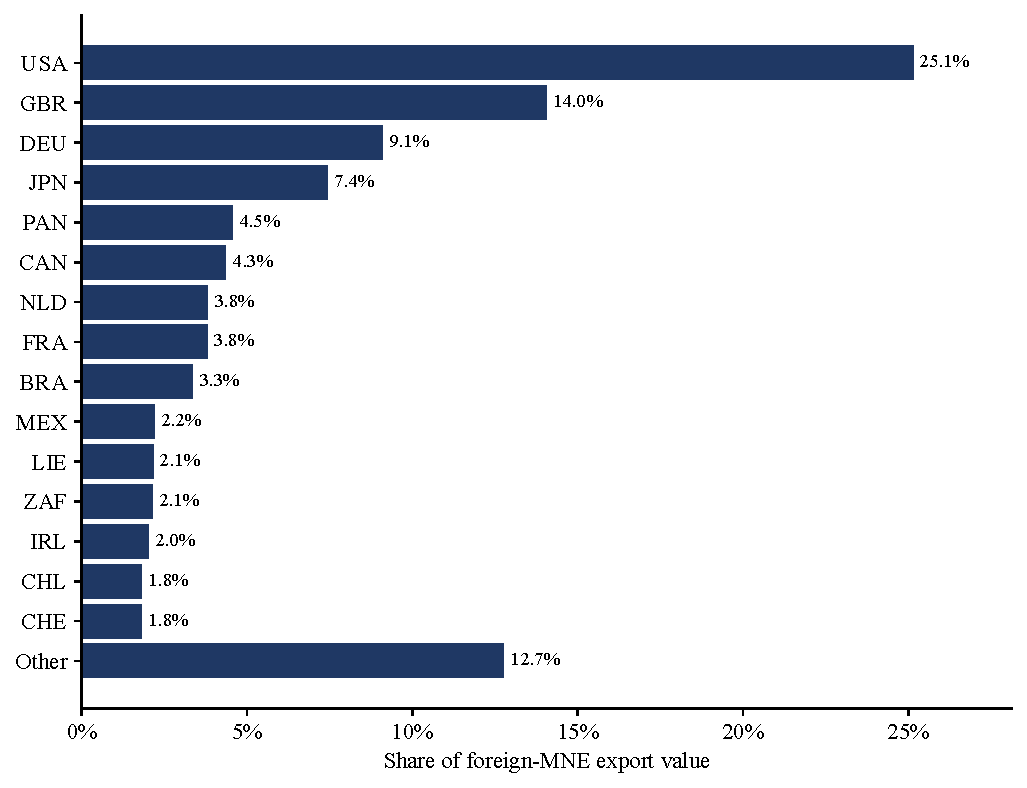
\includegraphics[width=0.78\textwidth,height=0.8\textheight,keepaspectratio]{figures/manufacturing/fig_wp1a_parent_share.pdf}%
  \caption{Manufacturing: Foreign-Multinational Exports, by Parent Country}%
  \label{fig:f4_manufacturing}%
  \par\vspace{2pt}%
  \parbox{0.92\textwidth}{\footnotesize %
  \textit{Notes:} Percent of foreign-MNE manufacturing export value, by country of the ultimate parent.\\[3pt]%
  \textit{Source:} Authors' calculations based on customs data matched to Orbis and Dun \& Bradstreet.}%
  \end{figure}
% ---- Table: Manufacturing: Foreign-Multinational Exports, by Parent Country
\begin{table}[H]\centering\small%
  \caption{Manufacturing: Foreign-Multinational Exports, by Parent Country}%
  \label{tab:f4n_manufacturing}%
  \adjustbox{max width=\textwidth, max totalheight=0.8\textheight}{\begin{tabular}{lrr}
\toprule
Parent country & Share (\%) & Value (US\$bn/yr) \\
\midrule
USA & 25.1 & 9.1 \\
GBR & 14.0 & 4.2 \\
DEU & 9.1 & 3.7 \\
JPN & 7.4 & 2.9 \\
PAN & 4.5 & 1.3 \\
CAN & 4.3 & 1.3 \\
NLD & 3.8 & 1.5 \\
FRA & 3.8 & 1.3 \\
BRA & 3.3 & 1.3 \\
MEX & 2.2 & 0.7 \\
LIE & 2.1 & 0.7 \\
ZAF & 2.1 & 0.7 \\
IRL & 2.0 & 0.9 \\
CHL & 1.8 & 0.7 \\
CHE & 1.8 & 0.7 \\
Other (143 countries) & 12.7 & 4.7 \\
\midrule
All foreign MNEs & 100.0 & 38.5 \\
\bottomrule
\end{tabular}
}%
  \par\vspace{3pt}%
  \begin{minipage}{0.95\textwidth}\footnotesize %
  \textit{Notes:} Percent of foreign-MNE manufacturing export value, by country of the ultimate parent. Values are annual averages in US\$ billion.\\[3pt]%
  \textit{Source:} Authors' calculations based on customs data matched to Orbis and Dun \& Bradstreet.%
  \end{minipage}%
  \end{table}
% ---- Figure: Manufacturing: Share of Total Exports, by Parent Country
\begin{figure}[H]\centering%
  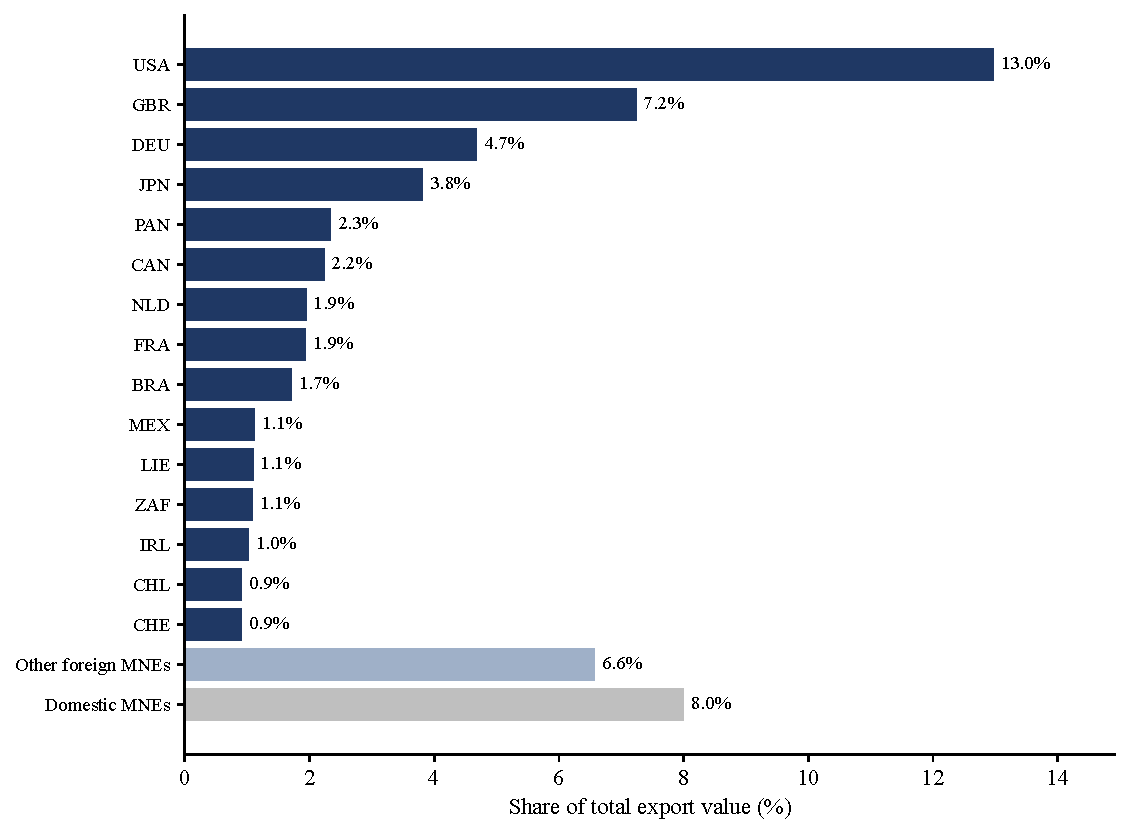
\includegraphics[width=0.85\textwidth,height=0.8\textheight,keepaspectratio]{figures/manufacturing/fig_wp1a_parent_share_total.pdf}%
  \caption{Manufacturing: Share of Total Exports, by Parent Country}%
  \label{fig:f4t_manufacturing}%
  \par\vspace{2pt}%
  \parbox{0.92\textwidth}{\footnotesize %
  \textit{Notes:} Percent of total manufacturing export value shipped by foreign MNEs of each parent country, other foreign MNEs and domestic MNEs; the remainder is local firms.\\[3pt]%
  \textit{Source:} Authors' calculations based on customs data matched to Orbis and Dun \& Bradstreet.}%
  \end{figure}
% ---- Table: Manufacturing: Share of Total Exports, by Parent Country
\begin{table}[H]\centering\small%
  \caption{Manufacturing: Share of Total Exports, by Parent Country}%
  \label{tab:f4tn_manufacturing}%
  \adjustbox{max width=\textwidth, max totalheight=0.8\textheight}{\begin{tabular}{lr}
\toprule
Exporter type / parent country & Share of total exports (\%) \\
\midrule
USA & 13.0 \\
GBR & 7.2 \\
DEU & 4.7 \\
JPN & 3.8 \\
PAN & 2.3 \\
CAN & 2.2 \\
NLD & 1.9 \\
FRA & 1.9 \\
BRA & 1.7 \\
MEX & 1.1 \\
LIE & 1.1 \\
ZAF & 1.1 \\
IRL & 1.0 \\
CHL & 0.9 \\
CHE & 0.9 \\
Other foreign MNEs & 6.6 \\
Domestic MNEs & 8.0 \\
\midrule
All MNEs & 59.6 \\
Local firms & 40.4 \\
\bottomrule
\end{tabular}
}%
  \par\vspace{3pt}%
  \begin{minipage}{0.95\textwidth}\footnotesize %
  \textit{Notes:} Percent of total manufacturing export value, by type of exporter and parent country.\\[3pt]%
  \textit{Source:} Authors' calculations based on customs data matched to Orbis and Dun \& Bradstreet.%
  \end{minipage}%
  \end{table}

\subsection{Parent Region and Destination Region}
% ---- Table: Manufacturing: Multinational Exports by Parent Region and Destination Region: Export Value
\begin{table}[H]\centering\small%
  \caption{Manufacturing: Multinational Exports by Parent Region and Destination Region: Export Value}%
  \label{tab:reg_value_manufacturing}%
  \adjustbox{max width=\textwidth, max totalheight=0.8\textheight}{\begin{tabular}{lrrrrrrrr}
\toprule
Parent region / Destination region & Latin America & North America & Europe & Asia & Africa & Oceania & Rest of World & Total \\
\midrule
Latin America & 3.1 & 0.8 & 0.5 & 1.2 & 0.1 & 0.0 & 0.0 & 5.6 \\
North America & 4.5 & 3.8 & 0.7 & 1.3 & 0.0 & 0.0 & 0.0 & 10.4 \\
Europe & 7.8 & 2.3 & 1.9 & 2.3 & 0.2 & 0.4 & 0.0 & 14.8 \\
Asia & 3.3 & 0.4 & 0.1 & 0.2 & 0.0 & 0.0 & 0.0 & 4.0 \\
Africa & 0.1 & 0.1 & 0.2 & 0.4 & 0.0 & 0.0 & 0.0 & 0.7 \\
Oceania & 0.0 & 0.0 & 0.0 & 0.1 & 0.0 & 0.0 & 0.0 & 0.1 \\
Rest of World & 0.0 & 0.0 & 0.0 & 0.0 & 0.0 & 0.0 & 0.0 & 0.0 \\
Domestic MNEs & 2.4 & 1.0 & 0.8 & 1.1 & 0.0 & 0.1 & 0.0 & 5.4 \\
Local firms & 11.9 & 6.1 & 3.7 & 6.6 & 0.3 & 0.1 & 0.1 & 28.8 \\
\midrule
Total & 33.2 & 14.5 & 7.8 & 13.1 & 0.6 & 0.6 & 0.1 & 69.8 \\
\bottomrule
\end{tabular}
}%
  \par\vspace{3pt}%
  \begin{minipage}{0.95\textwidth}\footnotesize %
  \textit{Notes:} Values are annual averages in US\$ billion. Rows: region of the ultimate parent; columns: destination region.\\[3pt]%
  \textit{Source:} Authors' calculations based on customs data matched to Orbis and Dun \& Bradstreet.%
  \end{minipage}%
  \end{table}
% ---- Table: Manufacturing: Multinational Exports by Parent Region and Destination Region: Row Percentages
\begin{table}[H]\centering\small%
  \caption{Manufacturing: Multinational Exports by Parent Region and Destination Region: Row Percentages}%
  \label{tab:reg_rowpct_manufacturing}%
  \adjustbox{max width=\textwidth, max totalheight=0.8\textheight}{\begin{tabular}{lrrrrrrrr}
\toprule
Parent region / Destination region & Latin America & North America & Europe & Asia & Africa & Oceania & Rest of World & Total \\
\midrule
Latin America & 53.0 & 14.1 & 8.2 & 23.2 & 0.9 & 0.2 & 0.4 & 100.0 \\
North America & 42.5 & 36.5 & 7.3 & 13.4 & 0.2 & 0.2 & 0.0 & 100.0 \\
Europe & 49.5 & 15.1 & 12.2 & 19.5 & 1.1 & 2.6 & 0.0 & 100.0 \\
Asia & 81.3 & 10.0 & 1.8 & 6.1 & 0.2 & 0.1 & 0.4 & 100.0 \\
Africa & 11.2 & 7.1 & 22.5 & 57.5 & 1.7 & 0.0 & 0.0 & 100.0 \\
Oceania & 33.7 & 11.5 & 14.9 & 39.3 & 0.2 & 0.3 & 0.0 & 100.0 \\
Rest of World & 71.1 & 0.7 & 4.0 & 0.7 & 0.0 & 23.5 & 0.1 & 100.0 \\
Domestic MNEs & 42.1 & 17.7 & 14.1 & 23.9 & 0.8 & 1.4 & 0.0 & 100.0 \\
Local firms & 39.2 & 21.2 & 12.9 & 25.2 & 0.9 & 0.3 & 0.2 & 100.0 \\
\bottomrule
\end{tabular}
}%
  \par\vspace{3pt}%
  \begin{minipage}{0.95\textwidth}\footnotesize %
  \textit{Notes:} Percent of each group's exports, by destination region (rows add to 100). Domestic MNEs and local firms are shown for comparison.\\[3pt]%
  \textit{Source:} Authors' calculations based on customs data matched to Orbis and Dun \& Bradstreet.%
  \end{minipage}%
  \end{table}
% ---- Table: Manufacturing: Multinational Exports by Parent Region and Destination Region: Column Percentages
\begin{table}[H]\centering\small%
  \caption{Manufacturing: Multinational Exports by Parent Region and Destination Region: Column Percentages}%
  \label{tab:reg_colpct_manufacturing}%
  \adjustbox{max width=\textwidth, max totalheight=0.8\textheight}{\begin{tabular}{lrrrrrrr}
\toprule
Parent region / Destination region & Latin America & North America & Europe & Asia & Africa & Oceania & Rest of World \\
\midrule
Latin America & 9.6 & 5.5 & 5.9 & 8.8 & 8.7 & 1.8 & 21.4 \\
North America & 13.8 & 26.0 & 9.5 & 9.1 & 3.0 & 2.8 & 1.8 \\
Europe & 22.7 & 15.2 & 22.4 & 18.8 & 27.5 & 63.4 & 5.7 \\
Asia & 9.1 & 2.4 & 0.8 & 1.4 & 1.4 & 0.8 & 11.2 \\
Africa & 0.3 & 0.4 & 2.2 & 3.0 & 2.4 & 0.0 & 0.0 \\
Oceania & 0.1 & 0.1 & 0.3 & 0.4 & 0.1 & 0.1 & 0.0 \\
Rest of World & 0.0 & 0.0 & 0.0 & 0.0 & 0.0 & 0.2 & 0.0 \\
Domestic MNEs & 7.8 & 7.2 & 10.4 & 9.2 & 8.3 & 13.7 & 2.4 \\
Local firms & 36.6 & 43.2 & 48.4 & 49.3 & 48.7 & 17.3 & 57.5 \\
\midrule
Total & 100.0 & 100.0 & 100.0 & 100.0 & 100.0 & 100.0 & 100.0 \\
\bottomrule
\end{tabular}
}%
  \par\vspace{3pt}%
  \begin{minipage}{0.95\textwidth}\footnotesize %
  \textit{Notes:} Percent of the exports reaching each destination region, by parent region (columns add to 100).\\[3pt]%
  \textit{Source:} Authors' calculations based on customs data matched to Orbis and Dun \& Bradstreet.%
  \end{minipage}%
  \end{table}
% ---- Figure: Manufacturing: Multinational Exports by Parent Region and Destination Region
\begin{figure}[H]\centering%
  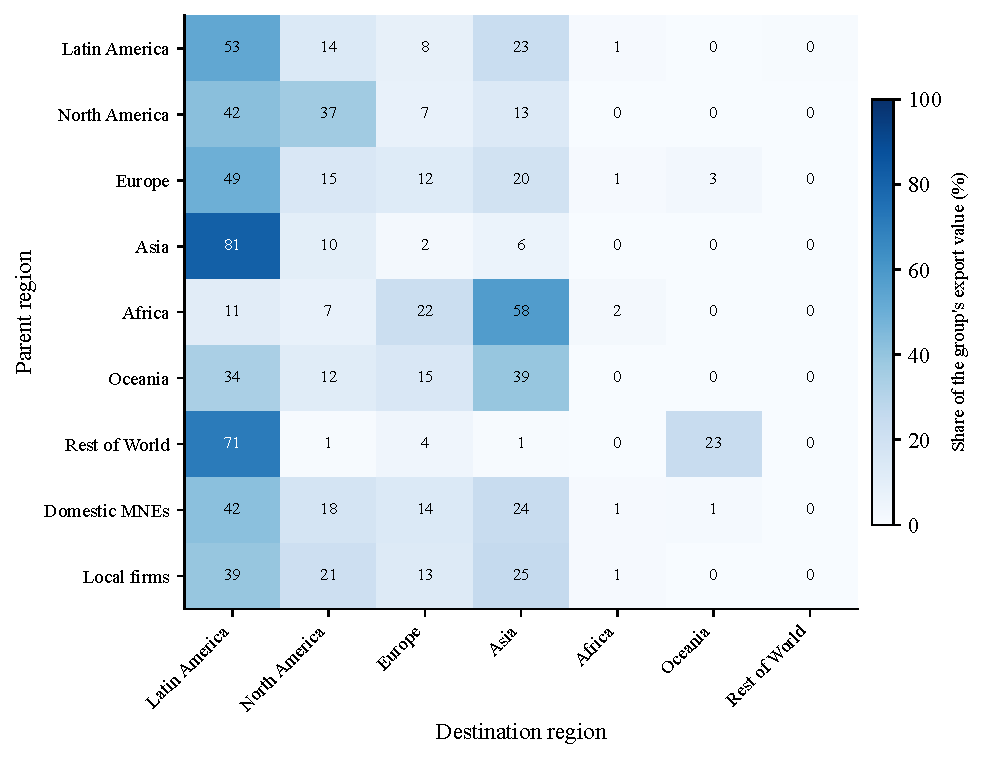
\includegraphics[width=0.9\textwidth,height=0.8\textheight,keepaspectratio]{figures/manufacturing/fig_wp1d_heatmap_region_rowpct.pdf}%
  \caption{Manufacturing: Multinational Exports by Parent Region and Destination Region}%
  \label{fig:reg_hm_manufacturing}%
  \par\vspace{2pt}%
  \parbox{0.92\textwidth}{\footnotesize %
  \textit{Notes:} Percent of each group's exports, by destination region (rows add to 100).\\[3pt]%
  \textit{Source:} Authors' calculations based on customs data matched to Orbis and Dun \& Bradstreet.}%
  \end{figure}
% ---- Table: Manufacturing: Foreign-Multinational Exports by Exporting Country and Destination Region
\begin{table}[H]\centering\small%
  \caption{Manufacturing: Foreign-Multinational Exports by Exporting Country and Destination Region}%
  \label{tab:odr_f_manufacturing}%
  \adjustbox{max width=\textwidth, max totalheight=0.8\textheight}{\begin{tabular}{lrrrrrrrr}
\toprule
Origin \ Destination region & Latin America & North America & Europe & Asia & Africa & Oceania & Rest of World & Total \\
\midrule
ARG & 78.8 & 4.5 & 9.7 & 3.9 & 1.5 & 1.7 & 0.0 & 13.1 \\
CHL & 19.1 & 16.4 & 11.3 & 50.5 & 0.2 & 2.5 & 0.0 & 6.4 \\
COL & 67.7 & 13.7 & 5.2 & 11.9 & 0.5 & 0.1 & 0.8 & 5.2 \\
CRI & 33.2 & 42.8 & 10.2 & 13.6 & 0.1 & 0.1 & 0.0 & 4.3 \\
DOM & 26.8 & 60.7 & 6.3 & 5.4 & 0.2 & 0.3 & 0.1 & 3.4 \\
PER & 43.5 & 22.1 & 18.0 & 14.9 & 1.2 & 0.3 & 0.0 & 2.5 \\
PRY & 79.5 & 7.2 & 9.4 & 3.9 & 0.1 & 0.0 & 0.0 & 0.4 \\
SLV & 43.0 & 55.7 & 0.8 & 0.4 & 0.1 & 0.1 & 0.0 & 2.0 \\
URY & 62.9 & 6.2 & 16.0 & 12.9 & 1.5 & 0.1 & 0.4 & 1.3 \\
\bottomrule
\end{tabular}
}%
  \par\vspace{3pt}%
  \begin{minipage}{0.95\textwidth}\footnotesize %
  \textit{Notes:} Percent of each country's foreign-MNE manufacturing exports, by destination region (rows add to 100). Last column: foreign-MNE exports. Values are annual averages in US\$ billion.\\[3pt]%
  \textit{Source:} Authors' calculations based on customs data matched to Orbis and Dun \& Bradstreet.%
  \end{minipage}%
  \end{table}
% ---- Table: Manufacturing: Local-Firm Exports by Exporting Country and Destination Region
\begin{table}[H]\centering\small%
  \caption{Manufacturing: Local-Firm Exports by Exporting Country and Destination Region}%
  \label{tab:odr_l_manufacturing}%
  \adjustbox{max width=\textwidth, max totalheight=0.8\textheight}{\begin{tabular}{lrrrrrrrr}
\toprule
Origin \ Destination region & Latin America & North America & Europe & Asia & Africa & Oceania & Rest of World & Total \\
\midrule
ARG & 56.3 & 16.3 & 13.4 & 11.2 & 2.5 & 0.3 & 0.0 & 7.3 \\
CHL & 14.5 & 16.9 & 16.6 & 51.0 & 0.4 & 0.6 & 0.0 & 7.3 \\
COL & 66.1 & 16.2 & 5.8 & 9.5 & 0.5 & 0.1 & 1.8 & 3.0 \\
CRI & 40.4 & 37.5 & 12.6 & 8.9 & 0.2 & 0.4 & 0.0 & 1.4 \\
DOM & 36.4 & 51.8 & 3.1 & 8.4 & 0.1 & 0.1 & 0.2 & 1.2 \\
PER & 40.4 & 19.7 & 16.0 & 23.1 & 0.3 & 0.4 & 0.0 & 5.3 \\
PRY & 69.5 & 4.7 & 15.0 & 10.6 & 0.1 & 0.0 & 0.0 & 0.6 \\
SLV & 46.4 & 51.1 & 0.9 & 1.5 & 0.1 & 0.0 & 0.0 & 1.8 \\
URY & 43.5 & 5.8 & 19.4 & 24.1 & 6.7 & 0.1 & 0.4 & 0.8 \\
\bottomrule
\end{tabular}
}%
  \par\vspace{3pt}%
  \begin{minipage}{0.95\textwidth}\footnotesize %
  \textit{Notes:} Percent of each country's manufacturing exports by local firms, by destination region (rows add to 100). Last column: local-firm exports. Values are annual averages in US\$ billion.\\[3pt]%
  \textit{Source:} Authors' calculations based on customs data matched to Orbis and Dun \& Bradstreet.%
  \end{minipage}%
  \end{table}

\subsection{Parent Country and Destination Country}
% ---- Table: Manufacturing: Foreign-Multinational Exports by Parent Country and Destination: Export Value
\begin{table}[H]\centering\small%
  \caption{Manufacturing: Foreign-Multinational Exports by Parent Country and Destination: Export Value}%
  \label{tab:cty_value_manufacturing}%
  \adjustbox{max width=\textwidth, max totalheight=0.8\textheight}{\begin{tabular}{lrrrrrrrrrrrr}
\toprule
Parent / Destination & BRA & USA & CHN & ECU & PER & CHL & MEX & NLD & KOR & VEN & Other destinations & Total \\
\midrule
USA & 1.5 & 3.6 & 0.2 & 0.2 & 0.2 & 0.2 & 0.2 & 0.3 & 0.0 & 0.1 & 2.4 & 9.1 \\
GBR & 0.4 & 0.6 & 1.3 & 0.0 & 0.0 & 0.1 & 0.1 & 0.1 & 0.3 & 0.0 & 1.2 & 4.2 \\
DEU & 1.5 & 0.3 & 0.0 & 0.1 & 0.1 & 0.1 & 0.2 & 0.0 & 0.0 & 0.0 & 1.3 & 3.7 \\
JPN & 1.7 & 0.2 & 0.0 & 0.1 & 0.1 & 0.1 & 0.0 & 0.0 & 0.0 & 0.0 & 0.7 & 2.9 \\
PAN & 0.0 & 0.1 & 0.5 & 0.0 & 0.0 & 0.0 & 0.0 & 0.0 & 0.1 & 0.0 & 0.5 & 1.3 \\
CAN & 0.1 & 0.1 & 0.4 & 0.0 & 0.0 & 0.0 & 0.0 & 0.0 & 0.1 & 0.0 & 0.5 & 1.3 \\
NLD & 1.1 & 0.0 & 0.0 & 0.0 & 0.0 & 0.0 & 0.0 & 0.0 & 0.0 & 0.0 & 0.3 & 1.5 \\
FRA & 0.5 & 0.0 & 0.0 & 0.1 & 0.1 & 0.1 & 0.2 & 0.0 & 0.0 & 0.0 & 0.3 & 1.3 \\
BRA & 0.3 & 0.2 & 0.1 & 0.1 & 0.0 & 0.1 & 0.0 & 0.0 & 0.0 & 0.0 & 0.6 & 1.3 \\
MEX & 0.2 & 0.1 & 0.0 & 0.0 & 0.0 & 0.0 & 0.0 & 0.0 & 0.0 & 0.0 & 0.3 & 0.7 \\
Other parents & 1.0 & 1.7 & 0.7 & 0.2 & 0.3 & 0.4 & 0.3 & 0.2 & 0.1 & 0.2 & 3.1 & 8.3 \\
\midrule
Total & 8.3 & 7.0 & 3.2 & 0.9 & 0.9 & 1.1 & 1.0 & 0.8 & 0.6 & 0.6 & 11.3 & 35.7 \\
\bottomrule
\end{tabular}
}%
  \par\vspace{3pt}%
  \begin{minipage}{0.95\textwidth}\footnotesize %
  \textit{Notes:} Values are annual averages in US\$ billion. Ten largest parent countries and ten largest destinations by foreign-MNE export value.\\[3pt]%
  \textit{Source:} Authors' calculations based on customs data matched to Orbis and Dun \& Bradstreet.%
  \end{minipage}%
  \end{table}
% ---- Table: Manufacturing: Foreign-Multinational Exports by Parent Country and Destination: Row Percentages
\begin{table}[H]\centering\small%
  \caption{Manufacturing: Foreign-Multinational Exports by Parent Country and Destination: Row Percentages}%
  \label{tab:cty_rowpct_manufacturing}%
  \adjustbox{max width=\textwidth, max totalheight=0.8\textheight}{\begin{tabular}{lrrrrrrrrrrrr}
\toprule
Parent / Destination & BRA & USA & CHN & ECU & PER & CHL & MEX & NLD & KOR & VEN & Other destinations & Total \\
\midrule
USA & 15.0 & 40.5 & 2.5 & 3.1 & 2.6 & 2.6 & 2.0 & 3.6 & 0.4 & 1.4 & 26.3 & 100.0 \\
GBR & 7.6 & 14.6 & 33.4 & 0.6 & 0.9 & 1.3 & 1.6 & 2.7 & 7.4 & 0.8 & 29.2 & 100.0 \\
DEU & 40.5 & 8.8 & 1.1 & 2.2 & 2.2 & 3.3 & 4.5 & 0.1 & 0.2 & 1.2 & 36.0 & 100.0 \\
JPN & 54.8 & 6.8 & 0.6 & 5.6 & 3.5 & 1.7 & 1.1 & 0.4 & 0.1 & 1.1 & 24.2 & 100.0 \\
PAN & 0.7 & 4.8 & 41.3 & 3.0 & 2.8 & 1.2 & 0.9 & 2.5 & 5.6 & 2.6 & 34.5 & 100.0 \\
CAN & 10.0 & 9.8 & 31.0 & 0.5 & 0.9 & 0.5 & 0.7 & 3.6 & 4.8 & 0.6 & 37.6 & 100.0 \\
NLD & 67.2 & 2.5 & 0.0 & 1.3 & 1.5 & 2.5 & 2.4 & 0.9 & 0.0 & 2.6 & 19.0 & 100.0 \\
FRA & 32.4 & 3.0 & 2.4 & 7.6 & 5.1 & 5.6 & 14.6 & 0.1 & 0.8 & 2.1 & 26.3 & 100.0 \\
BRA & 21.9 & 11.9 & 4.0 & 4.6 & 3.2 & 4.5 & 0.8 & 0.3 & 0.8 & 1.4 & 46.6 & 100.0 \\
MEX & 33.7 & 7.4 & 0.2 & 5.6 & 4.9 & 3.6 & 2.0 & 0.1 & 0.1 & 3.7 & 38.8 & 100.0 \\
Other parents & 11.4 & 20.0 & 9.3 & 3.0 & 4.1 & 4.0 & 3.4 & 2.7 & 1.8 & 2.8 & 37.4 & 100.0 \\
\bottomrule
\end{tabular}
}%
  \par\vspace{3pt}%
  \begin{minipage}{0.95\textwidth}\footnotesize %
  \textit{Notes:} Percent of each parent country's exports, by destination (rows add to 100). Ten largest parent countries and destinations.\\[3pt]%
  \textit{Source:} Authors' calculations based on customs data matched to Orbis and Dun \& Bradstreet.%
  \end{minipage}%
  \end{table}
% ---- Table: Manufacturing: Foreign-Multinational Exports by Parent Country and Destination: Column Percentages
\begin{table}[H]\centering\small%
  \caption{Manufacturing: Foreign-Multinational Exports by Parent Country and Destination: Column Percentages}%
  \label{tab:cty_colpct_manufacturing}%
  \adjustbox{max width=\textwidth, max totalheight=0.8\textheight}{\begin{tabular}{lrrrrrrrrrrr}
\toprule
Parent / Destination & BRA & USA & CHN & ECU & PER & CHL & MEX & NLD & KOR & VEN & Other destinations \\
\midrule
USA & 18.1 & 52.3 & 5.7 & 26.7 & 23.3 & 23.2 & 18.1 & 40.2 & 5.0 & 20.5 & 21.0 \\
GBR & 5.1 & 10.5 & 42.6 & 2.9 & 4.5 & 6.4 & 8.1 & 16.9 & 49.9 & 6.3 & 13.0 \\
DEU & 17.6 & 4.1 & 0.9 & 6.8 & 7.3 & 10.7 & 14.8 & 0.5 & 0.7 & 6.1 & 10.4 \\
JPN & 19.5 & 2.6 & 0.4 & 14.1 & 9.4 & 4.6 & 3.1 & 1.3 & 0.3 & 4.6 & 5.7 \\
PAN & 0.2 & 1.1 & 17.0 & 4.6 & 4.5 & 2.1 & 1.5 & 5.0 & 12.3 & 6.9 & 5.0 \\
CAN & 2.1 & 2.2 & 12.2 & 0.7 & 1.3 & 0.8 & 1.0 & 7.0 & 10.0 & 1.6 & 5.2 \\
NLD & 12.2 & 0.5 & 0.0 & 1.6 & 2.0 & 3.5 & 3.3 & 1.5 & 0.0 & 5.6 & 2.3 \\
FRA & 5.9 & 0.6 & 0.8 & 9.8 & 6.8 & 7.6 & 19.9 & 0.1 & 1.4 & 4.6 & 3.1 \\
BRA & 3.5 & 2.0 & 1.2 & 5.2 & 3.8 & 5.4 & 1.0 & 0.4 & 1.3 & 2.6 & 4.9 \\
MEX & 3.5 & 0.8 & 0.0 & 4.2 & 3.8 & 2.8 & 1.5 & 0.1 & 0.1 & 4.6 & 2.7 \\
Other parents & 12.4 & 23.2 & 19.1 & 23.4 & 33.2 & 33.0 & 27.7 & 26.8 & 19.1 & 36.5 & 26.7 \\
\midrule
Total & 100.0 & 100.0 & 100.0 & 100.0 & 100.0 & 100.0 & 100.0 & 100.0 & 100.0 & 100.0 & 100.0 \\
\bottomrule
\end{tabular}
}%
  \par\vspace{3pt}%
  \begin{minipage}{0.95\textwidth}\footnotesize %
  \textit{Notes:} Percent of the foreign-MNE exports reaching each destination, by parent country (columns add to 100). Ten largest parent countries and destinations.\\[3pt]%
  \textit{Source:} Authors' calculations based on customs data matched to Orbis and Dun \& Bradstreet.%
  \end{minipage}%
  \end{table}
% ---- Figure: Manufacturing: Destination of Foreign-Multinational Exports: Fifteen Largest Parent Countries and Destinations
\begin{figure}[H]\centering%
  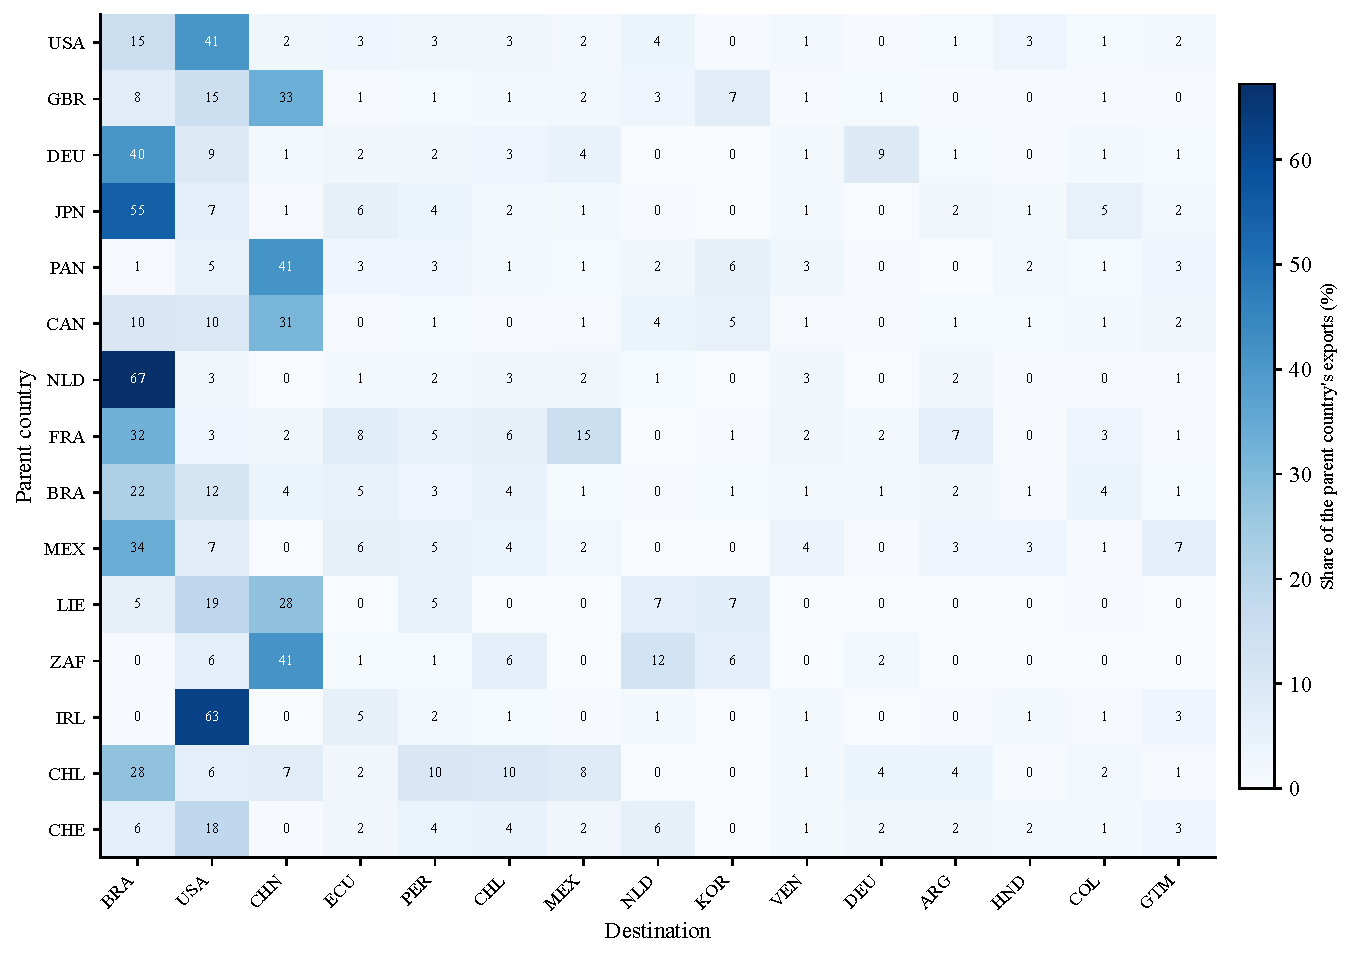
\includegraphics[width=1.0\textwidth,height=0.8\textheight,keepaspectratio]{figures/manufacturing/fig_wp1d_heatmap_country_rowpct.pdf}%
  \caption{Manufacturing: Destination of Foreign-Multinational Exports: Fifteen Largest Parent Countries and Destinations}%
  \label{fig:hm_row_manufacturing}%
  \par\vspace{2pt}%
  \parbox{0.92\textwidth}{\footnotesize %
  \textit{Notes:} Percent of each parent country's exports going to each destination (rows add to 100 including other destinations).\\[3pt]%
  \textit{Source:} Authors' calculations based on customs data matched to Orbis and Dun \& Bradstreet.}%
  \end{figure}
% ---- Figure: Manufacturing: Foreign-Multinational Exports by Parent Country and Destination: Share of the Total
\begin{figure}[H]\centering%
  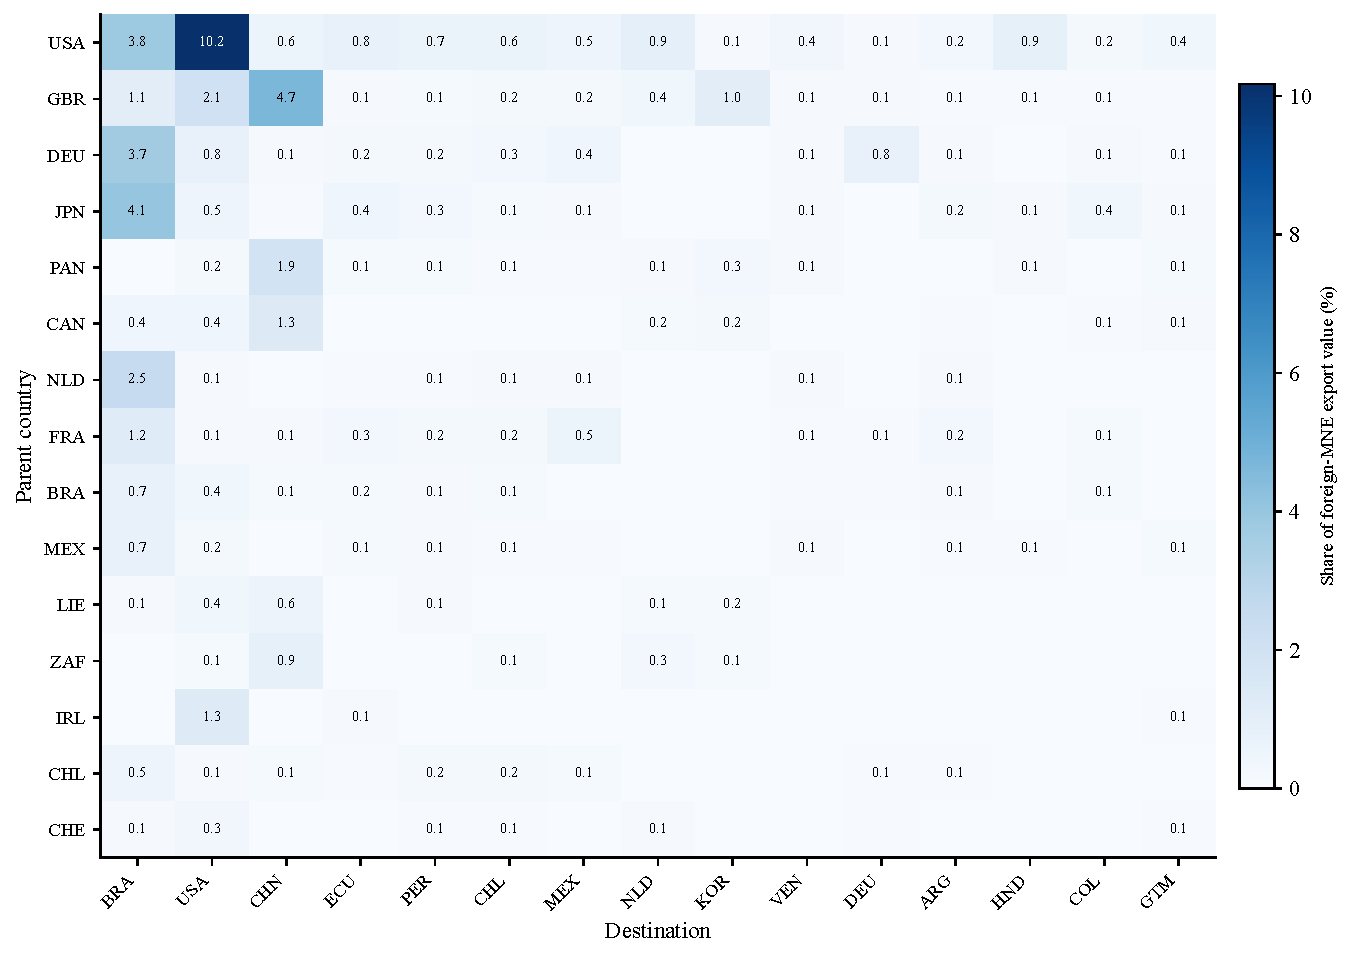
\includegraphics[width=1.0\textwidth,height=0.8\textheight,keepaspectratio]{figures/manufacturing/fig_wp1d_heatmap_country_cellpct.pdf}%
  \caption{Manufacturing: Foreign-Multinational Exports by Parent Country and Destination: Share of the Total}%
  \label{fig:hm_cell_manufacturing}%
  \par\vspace{2pt}%
  \parbox{0.92\textwidth}{\footnotesize %
  \textit{Notes:} Percent of all foreign-MNE export value in each parent country and destination pair; fifteen largest parent countries and destinations.\\[3pt]%
  \textit{Source:} Authors' calculations based on customs data matched to Orbis and Dun \& Bradstreet.}%
  \end{figure}

\subsection{Exports to the Parent Country}
% ---- Figure: Manufacturing: Share of Foreign-Multinational Exports Shipped to the Parent Country
\begin{figure}[H]\centering%
  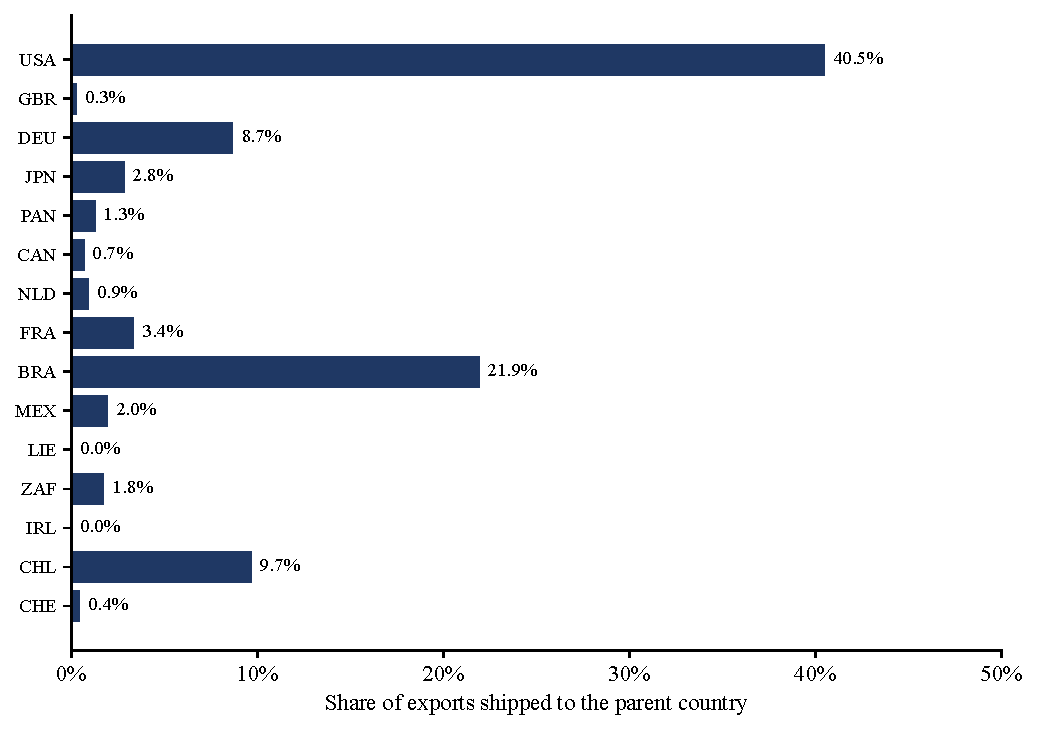
\includegraphics[width=0.85\textwidth,height=0.8\textheight,keepaspectratio]{figures/manufacturing/fig_wp1d_home_share_by_parent.pdf}%
  \caption{Manufacturing: Share of Foreign-Multinational Exports Shipped to the Parent Country}%
  \label{fig:home_manufacturing}%
  \par\vspace{2pt}%
  \parbox{0.92\textwidth}{\footnotesize %
  \textit{Notes:} Percent of each parent country's exports shipped to that same country.\\[3pt]%
  \textit{Source:} Authors' calculations based on customs data matched to Orbis and Dun \& Bradstreet.}%
  \end{figure}
% ---- Table: Manufacturing: Foreign-Multinational Exports to the Parent Countries, by Parent Country
\begin{table}[H]\centering\small%
  \caption{Manufacturing: Foreign-Multinational Exports to the Parent Countries, by Parent Country}%
  \label{tab:pxp_manufacturing}%
  \adjustbox{max width=\textwidth, max totalheight=0.8\textheight}{\begin{tabular}{lrrrrrrrrrrrr}
\toprule
Parent / Destination & USA & GBR & DEU & JPN & PAN & CAN & NLD & FRA & BRA & MEX & Other destinations & Total \\
\midrule
USA & 40.5 & 0.2 & 0.4 & 0.7 & 1.2 & 0.5 & 3.6 & 0.1 & 15.0 & 2.0 & 35.8 & 100.0 \\
GBR & 14.6 & 0.3 & 0.8 & 0.5 & 0.3 & 5.3 & 2.7 & 0.7 & 7.6 & 1.6 & 65.7 & 100.0 \\
DEU & 8.8 & 0.0 & 8.7 & 0.0 & 1.0 & 0.1 & 0.1 & 0.0 & 40.5 & 4.5 & 36.2 & 100.0 \\
JPN & 6.8 & 0.1 & 0.1 & 2.8 & 1.2 & 0.3 & 0.4 & 0.1 & 54.8 & 1.1 & 32.2 & 100.0 \\
PAN & 4.8 & 0.1 & 0.3 & 0.9 & 1.3 & 0.4 & 2.5 & 1.4 & 0.7 & 0.9 & 86.5 & 100.0 \\
CAN & 9.8 & 0.2 & 0.4 & 0.2 & 0.9 & 0.7 & 3.6 & 0.2 & 10.0 & 0.7 & 73.3 & 100.0 \\
NLD & 2.5 & 0.0 & 0.0 & 0.0 & 0.8 & 0.2 & 0.9 & 0.3 & 67.2 & 2.4 & 25.6 & 100.0 \\
FRA & 3.0 & 0.4 & 1.6 & 0.1 & 1.8 & 0.1 & 0.1 & 3.4 & 32.4 & 14.6 & 42.6 & 100.0 \\
BRA & 11.9 & 0.1 & 1.3 & 2.5 & 1.5 & 0.1 & 0.3 & 0.0 & 21.9 & 0.8 & 59.6 & 100.0 \\
MEX & 7.4 & 0.1 & 0.3 & 0.0 & 1.9 & 0.0 & 0.1 & 0.0 & 33.7 & 2.0 & 54.5 & 100.0 \\
Other parents & 20.0 & 0.6 & 2.5 & 1.0 & 2.1 & 0.6 & 2.7 & 0.3 & 11.4 & 3.4 & 55.3 & 100.0 \\
\bottomrule
\end{tabular}
}%
  \par\vspace{3pt}%
  \begin{minipage}{0.95\textwidth}\footnotesize %
  \textit{Notes:} Percent of each parent country's exports, by destination (rows add to 100). Destinations are the ten largest parent countries; the diagonal is the share shipped to the parent's own country.\\[3pt]%
  \textit{Source:} Authors' calculations based on customs data matched to Orbis and Dun \& Bradstreet.%
  \end{minipage}%
  \end{table}
% ---- Figure: Manufacturing: Share of Foreign-Multinational Exports Shipped to the Parent Jurisdiction, Consolidated Parents
\begin{figure}[H]\centering%
  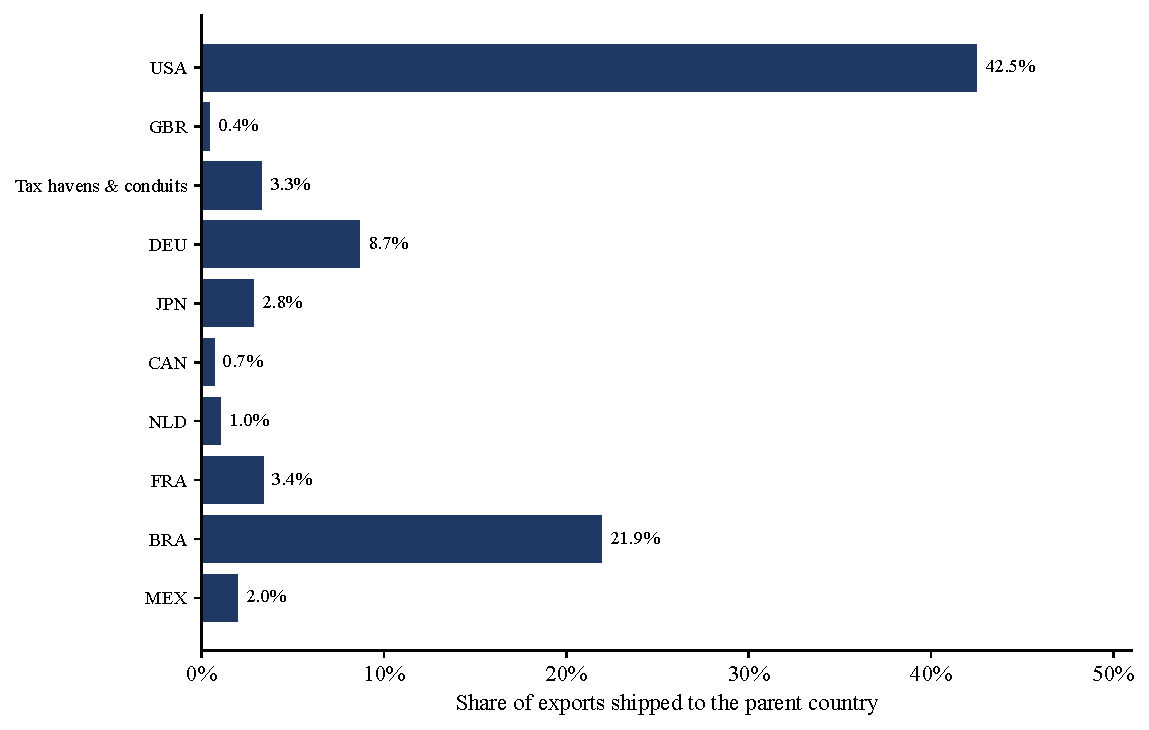
\includegraphics[width=0.85\textwidth,height=0.8\textheight,keepaspectratio]{figures/manufacturing/fig_wp1d_home_share_by_parent_consolidated.pdf}%
  \caption{Manufacturing: Share of Foreign-Multinational Exports Shipped to the Parent Jurisdiction, Consolidated Parents}%
  \label{fig:homec_manufacturing}%
  \par\vspace{2pt}%
  \parbox{0.92\textwidth}{\footnotesize %
  \textit{Notes:} Percent of each parent's exports shipped to its own jurisdiction. Dependencies are assigned to their sovereign state and tax havens and conduit jurisdictions are pooled.\\[3pt]%
  \textit{Source:} Authors' calculations based on customs data matched to Orbis and Dun \& Bradstreet.}%
  \end{figure}
% ---- Table: Manufacturing: Share of Foreign-Multinational Exports Shipped to the Parent Jurisdiction, Consolidated Parents
\begin{table}[H]\centering\small%
  \caption{Manufacturing: Share of Foreign-Multinational Exports Shipped to the Parent Jurisdiction, Consolidated Parents}%
  \label{tab:homec_t_manufacturing}%
  \adjustbox{max width=\textwidth, max totalheight=0.8\textheight}{\begin{tabular}{lrr}
\toprule
Consolidated parent & Home share (\%) & Exports (US\$bn/yr) \\
\midrule
USA & 42.5 & 9.1 \\
GBR & 0.4 & 4.9 \\
Tax havens \& conduits & 3.3 & 4.3 \\
DEU & 8.7 & 3.7 \\
JPN & 2.8 & 2.9 \\
CAN & 0.7 & 1.3 \\
NLD & 1.0 & 1.6 \\
FRA & 3.4 & 1.3 \\
BRA & 21.9 & 1.3 \\
MEX & 2.0 & 0.7 \\
\bottomrule
\end{tabular}
}%
  \par\vspace{3pt}%
  \begin{minipage}{0.95\textwidth}\footnotesize %
  \textit{Notes:} Home share: percent of the parent's exports shipped to its own jurisdiction. Values are annual averages in US\$ billion.\\[3pt]%
  \textit{Source:} Authors' calculations based on customs data matched to Orbis and Dun \& Bradstreet.%
  \end{minipage}%
  \end{table}
% ---- Figure: Manufacturing: Share of Foreign-Multinational Exports Shipped to the Parent Jurisdiction
\begin{figure}[H]\centering%
  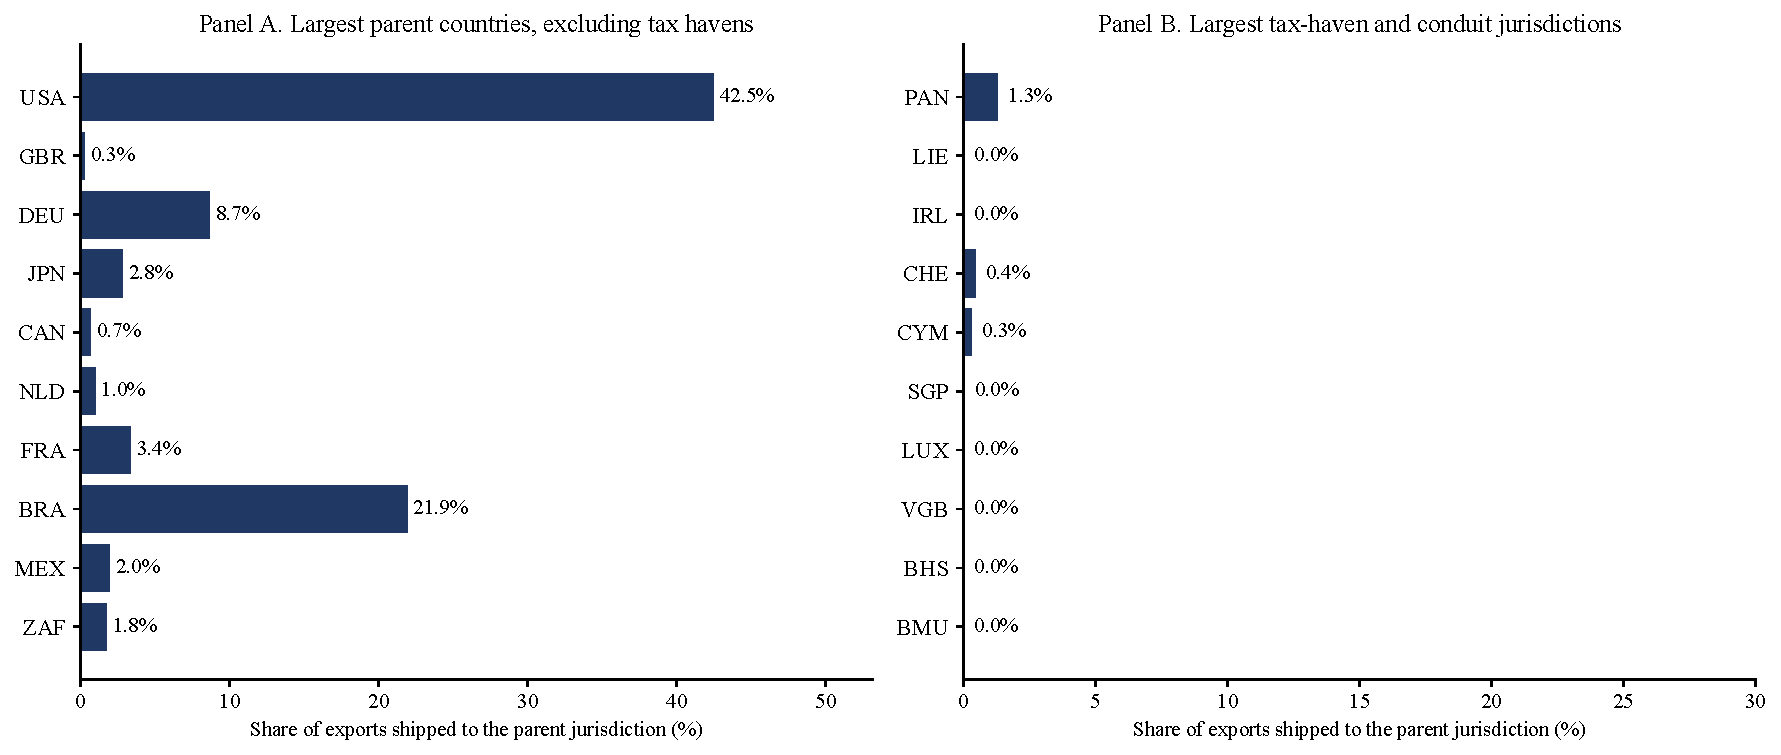
\includegraphics[width=1.0\textwidth,height=0.8\textheight,keepaspectratio]{figures/manufacturing/fig_wp1d_home_share_haven_panels.pdf}%
  \caption{Manufacturing: Share of Foreign-Multinational Exports Shipped to the Parent Jurisdiction}%
  \label{fig:homeh_manufacturing}%
  \par\vspace{2pt}%
  \parbox{0.92\textwidth}{\footnotesize %
  \textit{Notes:} Percent of each parent jurisdiction's exports shipped to that same jurisdiction. Panel A: largest parent countries, excluding tax havens; dependencies are assigned to their sovereign state. Panel B: largest tax-haven and conduit jurisdictions.\\[3pt]%
  \textit{Source:} Authors' calculations based on customs data matched to Orbis and Dun \& Bradstreet.}%
  \end{figure}
% ---- Table: Manufacturing: Share of Foreign-Multinational Exports Shipped to the Parent Jurisdiction
\begin{table}[H]\centering\small%
  \caption{Manufacturing: Share of Foreign-Multinational Exports Shipped to the Parent Jurisdiction}%
  \label{tab:homeh_t_manufacturing}%
  \adjustbox{max width=\textwidth, max totalheight=0.8\textheight}{\begin{tabular}{llrr}
\toprule
Panel & Parent & Home share (\%) & Exports (US\$bn/yr) \\
\midrule
Panel A & USA & 42.5 & 9.1 \\
Panel A & GBR & 0.3 & 4.2 \\
Panel A & DEU & 8.7 & 3.7 \\
Panel A & JPN & 2.8 & 2.9 \\
Panel A & CAN & 0.7 & 1.3 \\
Panel A & NLD & 1.0 & 1.5 \\
Panel A & FRA & 3.4 & 1.3 \\
Panel A & BRA & 21.9 & 1.3 \\
Panel A & MEX & 2.0 & 0.7 \\
Panel A & ZAF & 1.8 & 0.7 \\
\midrule
Panel B & PAN & 1.3 & 1.3 \\
Panel B & LIE & 0.0 & 0.7 \\
Panel B & IRL & 0.0 & 0.9 \\
Panel B & CHE & 0.4 & 0.7 \\
Panel B & CYM & 0.3 & 0.3 \\
Panel B & SGP & 0.0 & 0.3 \\
Panel B & LUX & 0.0 & 0.2 \\
Panel B & VGB & 0.0 & 0.2 \\
Panel B & BHS & 0.0 & 0.2 \\
Panel B & BMU & 0.0 & 0.2 \\
\bottomrule
\end{tabular}
}%
  \par\vspace{3pt}%
  \begin{minipage}{0.95\textwidth}\footnotesize %
  \textit{Notes:} Home share: percent of the parent's exports shipped to its own jurisdiction. Panel A: largest parent countries, excluding tax havens. Panel B: largest tax-haven and conduit jurisdictions. Values are annual averages in US\$ billion.\\[3pt]%
  \textit{Source:} Authors' calculations based on customs data matched to Orbis and Dun \& Bradstreet.%
  \end{minipage}%
  \end{table}

\subsection{Destination Markets}
% ---- Figure: Manufacturing: Exports to the United States, by Type of Exporter and Exporting Country
\begin{figure}[H]\centering%
  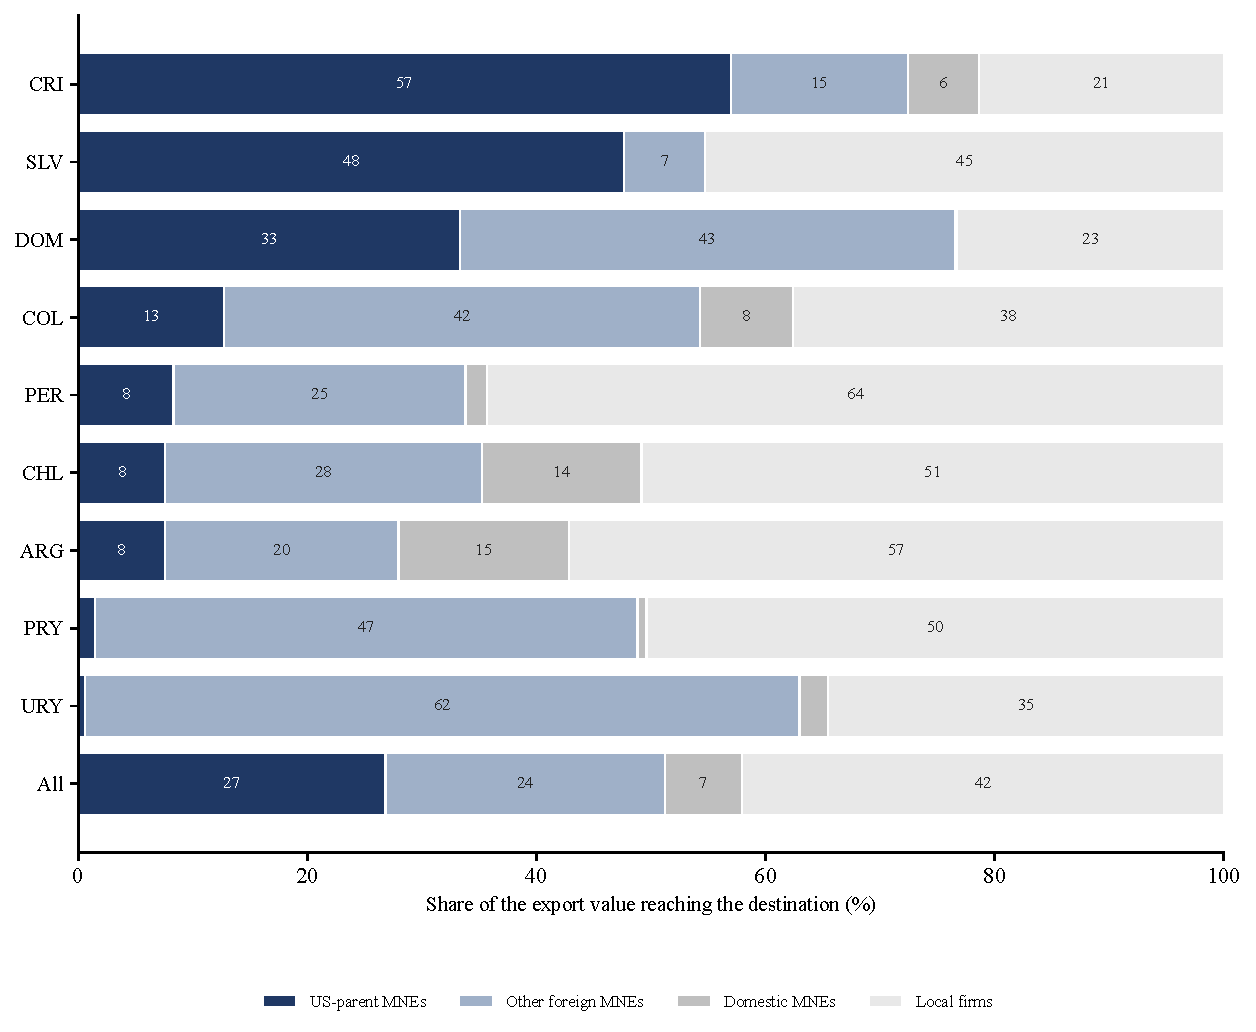
\includegraphics[width=0.9\textwidth,height=0.8\textheight,keepaspectratio]{figures/manufacturing/fig_wp3_to_usa_carriers.pdf}%
  \caption{Manufacturing: Exports to the United States, by Type of Exporter and Exporting Country}%
  \label{fig:to_usa_f_manufacturing}%
  \par\vspace{2pt}%
  \parbox{0.92\textwidth}{\footnotesize %
  \textit{Notes:} Percent of each country's manufacturing exports to the United States, by type of exporter.\\[3pt]%
  \textit{Source:} Authors' calculations based on customs data matched to Orbis and Dun \& Bradstreet.}%
  \end{figure}
% ---- Table: Manufacturing: Exports to the United States, by Type of Exporter and Exporting Country
\begin{table}[H]\centering\small%
  \caption{Manufacturing: Exports to the United States, by Type of Exporter and Exporting Country}%
  \label{tab:to_usa_manufacturing}%
  \adjustbox{max width=\textwidth, max totalheight=0.8\textheight}{\begin{tabular}{lrrrrr}
\toprule
Origin & Exports to the USA (US\$bn/yr) & US-parent MNEs (\%) & Other foreign MNEs (\%) & Domestic MNEs (\%) & Local firms (\%) \\
\midrule
CRI & 2.5 & 57.0 & 15.5 & 6.2 & 21.4 \\
SLV & 2.0 & 47.7 & 7.1 & 0.0 & 45.3 \\
DOM & 2.7 & 33.3 & 43.2 & 0.2 & 23.3 \\
COL & 1.3 & 12.7 & 41.5 & 8.1 & 37.6 \\
PER & 1.6 & 8.3 & 25.5 & 1.9 & 64.3 \\
CHL & 2.4 & 7.6 & 27.6 & 14.0 & 50.8 \\
ARG & 2.0 & 7.6 & 20.4 & 14.9 & 57.2 \\
PRY & 0.1 & 1.4 & 47.4 & 0.8 & 50.4 \\
URY & 0.1 & 0.6 & 62.4 & 2.5 & 34.5 \\
\midrule
All & 14.5 & 26.8 & 24.4 & 6.7 & 42.1 \\
\bottomrule
\end{tabular}
}%
  \par\vspace{3pt}%
  \begin{minipage}{0.95\textwidth}\footnotesize %
  \textit{Notes:} Percent of each country's manufacturing exports to the United States, by type of exporter. Values are annual averages in US\$ billion.\\[3pt]%
  \textit{Source:} Authors' calculations based on customs data matched to Orbis and Dun \& Bradstreet.%
  \end{minipage}%
  \end{table}
% ---- Figure: Manufacturing: Ownership of Exports to the Main Destination Markets
\begin{figure}[H]\centering%
  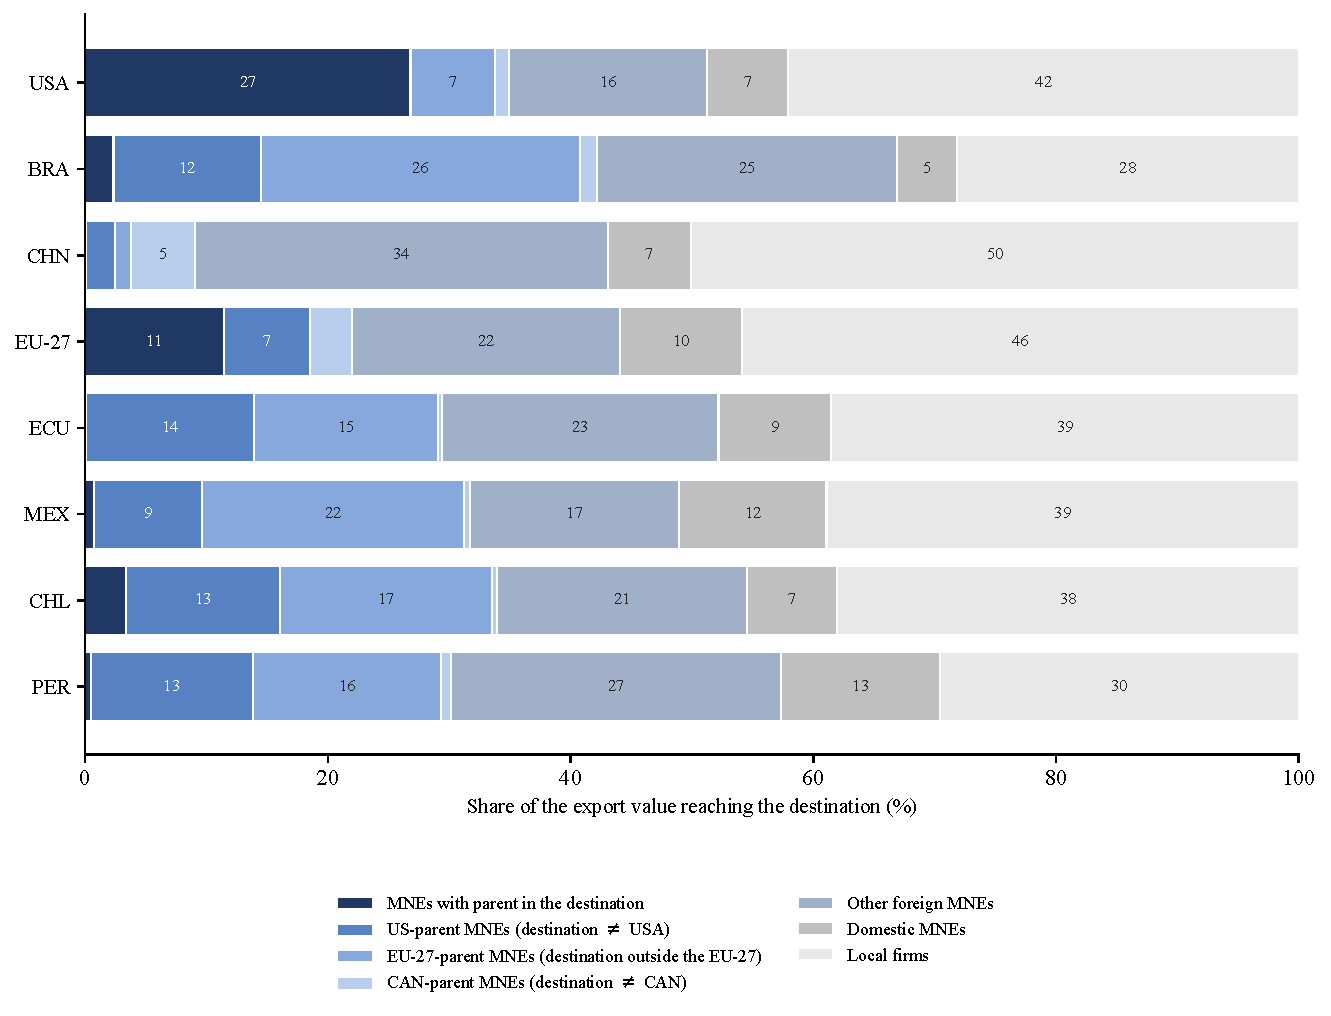
\includegraphics[width=0.95\textwidth,height=0.8\textheight,keepaspectratio]{figures/manufacturing/fig_wp3_dest_carriers.pdf}%
  \caption{Manufacturing: Ownership of Exports to the Main Destination Markets}%
  \label{fig:dest_f_manufacturing}%
  \par\vspace{2pt}%
  \parbox{0.92\textwidth}{\footnotesize %
  \textit{Notes:} Percent of the export value reaching each destination, by type of exporter. The first segment is exports by MNEs whose parent is located in that destination. EU-27 member states are pooled.\\[3pt]%
  \textit{Source:} Authors' calculations based on customs data matched to Orbis and Dun \& Bradstreet.}%
  \end{figure}
% ---- Table: Manufacturing: Ownership of Exports to the Main Destination Markets
\begin{table}[H]\centering\footnotesize%
  \caption{Manufacturing: Ownership of Exports to the Main Destination Markets}%
  \label{tab:dest_manufacturing}%
  \adjustbox{max width=\textwidth, max totalheight=0.8\textheight}{\begin{tabular}{lrrrrrrrr}
\toprule
Destination & \multicolumn{1}{p{1.5cm}}{\raggedright Exports (US\$bn/yr)} & \multicolumn{1}{p{2.2cm}}{\raggedright MNEs with parent in the destination (\%)} & \multicolumn{1}{p{1.6cm}}{\raggedright US-parent MNEs (\%)} & \multicolumn{1}{p{1.6cm}}{\raggedright EU-27-parent MNEs (\%)} & \multicolumn{1}{p{1.6cm}}{\raggedright CAN-parent MNEs (\%)} & \multicolumn{1}{p{1.6cm}}{\raggedright Other foreign MNEs (\%)} & \multicolumn{1}{p{1.6cm}}{\raggedright Domestic MNEs (\%)} & \multicolumn{1}{p{1.5cm}}{\raggedright Local firms (\%)} \\
\midrule
USA & 14.5 & 26.8 & -- & 7.0 & 1.1 & 16.3 & 6.7 & 42.1 \\
BRA & 12.4 & 2.3 & 12.1 & 26.3 & 1.4 & 24.7 & 4.9 & 28.2 \\
CHN & 7.7 & 0.0 & 2.5 & 1.3 & 5.3 & 34.0 & 6.8 & 50.1 \\
EU-27 & 7.3 & 11.4 & 7.1 & -- & 3.4 & 22.1 & 10.0 & 45.9 \\
ECU & 2.2 & 0.0 & 13.9 & 15.1 & 0.4 & 22.7 & 9.3 & 38.5 \\
MEX & 2.2 & 0.8 & 8.9 & 21.6 & 0.5 & 17.2 & 12.1 & 38.9 \\
CHL & 2.2 & 3.4 & 12.7 & 17.5 & 0.4 & 20.6 & 7.4 & 38.1 \\
PER & 1.8 & 0.5 & 13.4 & 15.5 & 0.8 & 27.2 & 13.1 & 29.5 \\
\bottomrule
\end{tabular}
}%
  \par\vspace{3pt}%
  \begin{minipage}{0.95\textwidth}\footnotesize %
  \textit{Notes:} Percent of the export value reaching each destination, by type of exporter. EU-27 member states are pooled. Values are annual averages in US\$ billion.\\[3pt]%
  \textit{Source:} Authors' calculations based on customs data matched to Orbis and Dun \& Bradstreet.%
  \end{minipage}%
  \end{table}
% ---- Table: Manufacturing: Main Products Shipped by US-Parent Multinationals to the United States
\begin{table}[H]\centering\footnotesize%
  \caption{Manufacturing: Main Products Shipped by US-Parent Multinationals to the United States}%
  \label{tab:us_home_manufacturing}%
  \adjustbox{max width=\textwidth, max totalheight=0.8\textheight}{\begin{tabular}{llrrrrrl}
\toprule
HS6 & Description & \multicolumn{1}{p{1.7cm}}{\raggedright US-parent exports to the USA (US\$bn/yr)} & \multicolumn{1}{p{1.7cm}}{\raggedright \% of all US-parent exports to the USA} & \multicolumn{1}{p{2.0cm}}{\raggedright \% of US-parent exports of the product going to the USA} & \multicolumn{1}{p{1.9cm}}{\raggedright All exports of the product to the USA (US\$bn/yr)} & \multicolumn{1}{p{2.2cm}}{\raggedright US-parent share of exports of the product to the USA (\%)} & \multicolumn{1}{p{2.6cm}}{\raggedright Main origins of the US-parent shipments (\% of the line)} \\
\midrule
610910 & T-shirts, singlets \& other vests, knitted/cro... & 0.49 & 15.4 & 84 & 1.01 & 53 & SLV 85\%, DOM 10\%, PER 5\% \\
901839 & Catheters, cannulae \& the like & 0.52 & 13.4 & 73 & 0.63 & 89 & CRI 92\%, DOM 8\%, COL 0\% \\
901890 & Instruments \& appliances used in medical/surg... & 0.39 & 9.5 & 69 & 0.94 & 47 & CRI 71\%, DOM 29\%, COL 0\% \\
854231 & Electronic integrated circuits, processors \& ... & 0.21 & 5.4 & 28 & 0.22 & 95 & CRI 100\%, COL 0\%, ARG 0\% \\
401110 & New pneumatic tyres, of rubber, of a kind use... & 0.13 & 4.8 & 93 & 0.24 & 63 & CHL 100\%, DOM 0\%, COL 0\% \\
611595 & Other n.e.s. in 61.15, knitted/crocheted, of ... & 0.10 & 3.3 & 100 & 0.11 & 97 & SLV 100\%, DOM 0\% \\
610711 & Men's/boys' underpants \& briefs, knitted/croc... & 0.09 & 3.0 & 87 & 0.10 & 87 & SLV 100\%, DOM 0\%, CRI 0\% \\
621210 & Brassieres \& parts thereof , whether/not knit... & 0.09 & 2.5 & 98 & 0.12 & 78 & SLV 74\%, DOM 26\%, CRI 0\% \\
740311 & Cathodes \& sections of cathodes, of refined c... & 0.06 & 1.6 & 24 & 1.56 & 3 & PER 64\%, CHL 36\% \\
640510 & Footwear with uppers of leather/composition l... & 0.08 & 1.6 & 70 & 0.11 & 71 & DOM 100\% \\
392690 & Articles of plastics\&articles of other materi... & 0.06 & 1.5 & 79 & 0.08 & 77 & CRI 66\%, DOM 33\%, SLV 0\% \\
620711 & Men's/boys' underpants \& briefs (excl. knitte... & 0.04 & 1.2 & 99 & 0.05 & 99 & CRI 73\%, SLV 27\%, DOM 0\% \\
611521 & Panty hose, tights, stockings, socks \& other ... & 0.03 & 1.1 & 77 & 0.03 & 98 & SLV 100\%, DOM 0\% \\
630790 & Other made-up textile articles, incl. dress p... & 0.05 & 1.1 & 97 & 0.06 & 90 & DOM 100\%, COL 0\%, CRI 0\% \\
611596 & Other n.e.s. in 61.15, knitted/crocheted, of ... & 0.03 & 1.1 & 100 & 0.04 & 87 & SLV 100\%, CRI 0\%, PER 0\% \\
\midrule
All lines & & 3.6 & 100.0 & 41 & 14.5 & 27 & \\
\bottomrule
\end{tabular}
}%
  \par\vspace{3pt}%
  \begin{minipage}{0.95\textwidth}\footnotesize %
  \textit{Notes:} Fifteen HS6 products with the largest exports by US-parent MNEs to the United States. Values are annual averages in US\$ billion.\\[3pt]%
  \textit{Source:} Authors' calculations based on customs data matched to Orbis and Dun \& Bradstreet.%
  \end{minipage}%
  \end{table}
% ---- Figure: Manufacturing: US-Parent Share of Exports to the United States, Main Products Shipped by US-Parent Multinationals
\begin{figure}[H]\centering%
  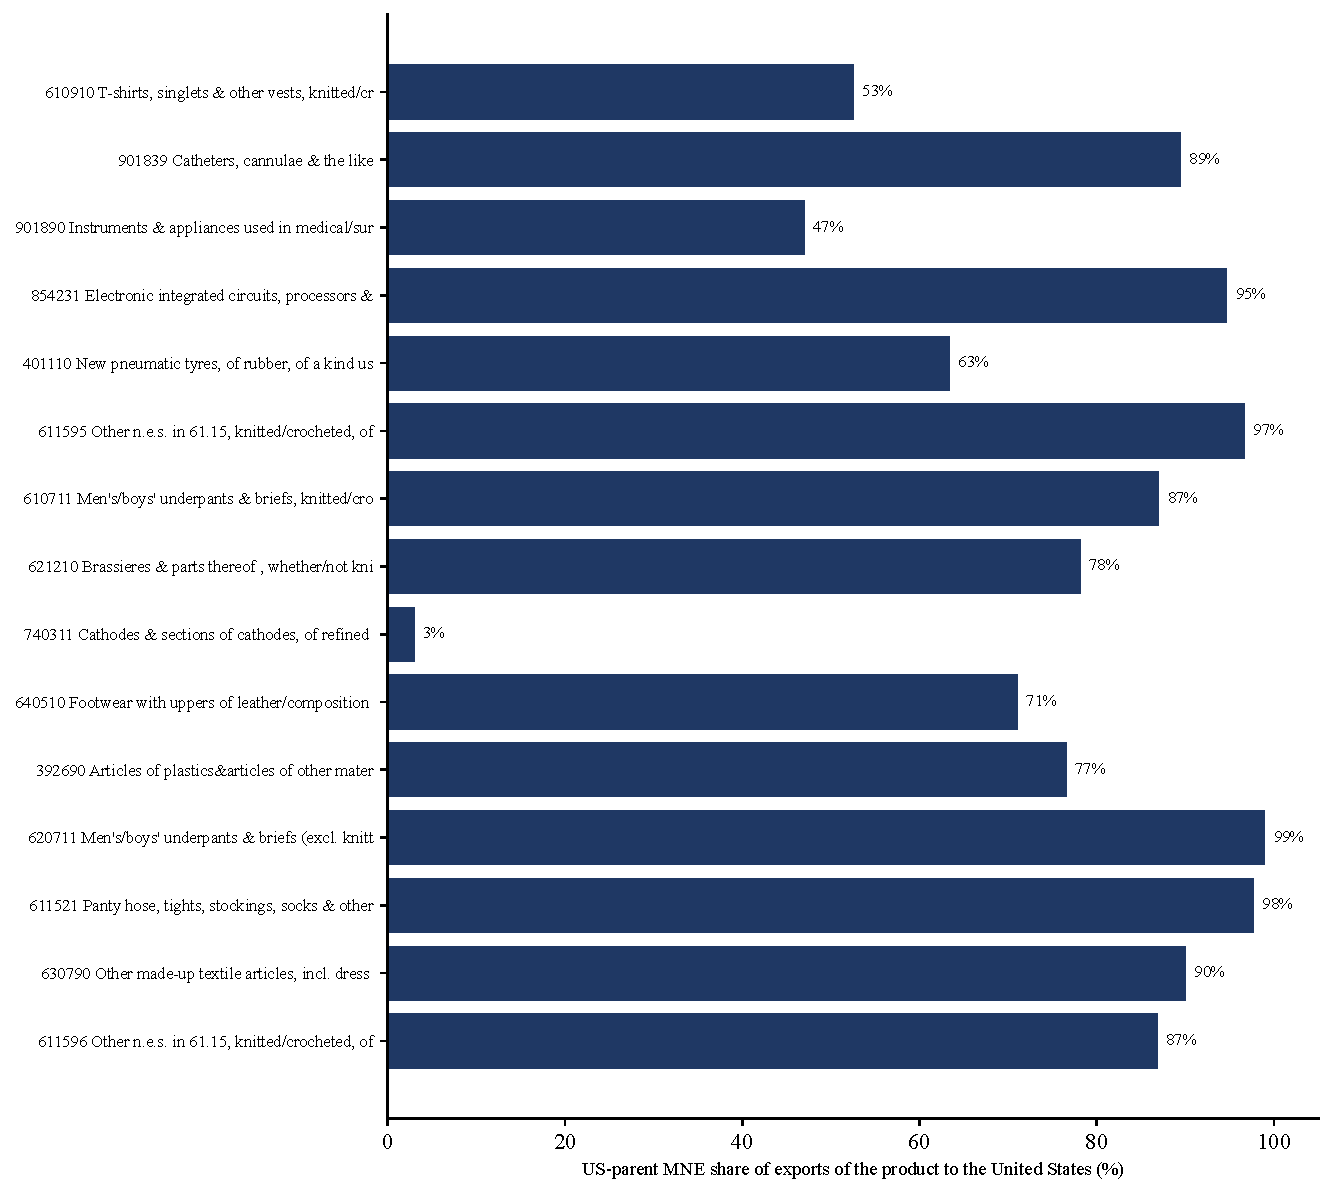
\includegraphics[width=0.95\textwidth,height=0.8\textheight,keepaspectratio]{figures/manufacturing/fig_wp3_us_home_products.pdf}%
  \caption{Manufacturing: US-Parent Share of Exports to the United States, Main Products Shipped by US-Parent Multinationals}%
  \label{fig:us_home_f_manufacturing}%
  \par\vspace{2pt}%
  \parbox{0.92\textwidth}{\footnotesize %
  \textit{Notes:} Percent of the nine countries' exports of each product to the United States shipped by US-parent MNEs; the fifteen products with the largest US-parent exports to the United States.\\[3pt]%
  \textit{Source:} Authors' calculations based on customs data matched to Orbis and Dun \& Bradstreet.}%
  \end{figure}
% ---- Table: Manufacturing: Largest Export Products to the United States, by Type of Exporter
\begin{table}[H]\centering\footnotesize%
  \caption{Manufacturing: Largest Export Products to the United States, by Type of Exporter}%
  \label{tab:to_usa_prod_manufacturing}%
  \adjustbox{max width=\textwidth, max totalheight=0.8\textheight}{\begin{tabular}{llrrrrr}
\toprule
HS6 & Description & \multicolumn{1}{p{2.0cm}}{\raggedright Exports to the USA (US\$bn/yr)} & \multicolumn{1}{p{1.8cm}}{\raggedright US-parent MNEs (\%)} & \multicolumn{1}{p{1.8cm}}{\raggedright Other foreign MNEs (\%)} & \multicolumn{1}{p{1.8cm}}{\raggedright Domestic MNEs (\%)} & \multicolumn{1}{p{1.8cm}}{\raggedright Local firms (\%)} \\
\midrule
740311 & Cathodes \& sections of cathodes, of refined c... & 1.56 & 3 & 33 & 4 & 60 \\
610910 & T-shirts, singlets \& other vests, knitted/cro... & 1.01 & 53 & 7 & 0 & 40 \\
901890 & Instruments \& appliances used in medical/surg... & 0.94 & 47 & 44 & 0 & 9 \\
901839 & Catheters, cannulae \& the like & 0.63 & 89 & 2 & 0 & 9 \\
401110 & New pneumatic tyres, of rubber, of a kind use... & 0.24 & 63 & 16 & 0 & 20 \\
853620 & Automatic circuit breakers, for a voltage not... & 0.35 & 9 & 91 & 0 & 0 \\
382490 & Chemical products\&preparations of the chemica... & 0.30 & 0 & 36 & 14 & 50 \\
854231 & Electronic integrated circuits, processors \& ... & 0.22 & 95 & 4 & 0 & 2 \\
880240 & Aeroplanes \& other aircraft, of an unladen we... & 0.21 & 0 & 6 & 83 & 11 \\
902139 & Artificial parts of the body other than teeth... & 0.19 & 5 & 1 & 70 & 25 \\
800110 & Tin, not alloyed, unwrought & 0.19 & 0 & 0 & 0 & 100 \\
611020 & Jerseys, pullovers, cardigans, waist-coats \& ... & 0.15 & 23 & 7 & 0 & 70 \\
610990 & T-shirts, singlets \& other vests, knitted/cro... & 0.14 & 25 & 12 & 1 & 62 \\
853221 & Fixed electrical capacitors, other than those... & 0.12 & 0 & 0 & 0 & 100 \\
611030 & Jerseys, pullovers, cardigans, waist-coats \& ... & 0.13 & 11 & 21 & 0 & 68 \\
\bottomrule
\end{tabular}
}%
  \par\vspace{3pt}%
  \begin{minipage}{0.95\textwidth}\footnotesize %
  \textit{Notes:} Fifteen largest HS6 products exported to the United States; percent of each product's exports to the United States by type of exporter. Values are annual averages in US\$ billion.\\[3pt]%
  \textit{Source:} Authors' calculations based on customs data matched to Orbis and Dun \& Bradstreet.%
  \end{minipage}%
  \end{table}

\section{Fact 4: A Small Set of Large Multinational Groups Accounts for Most Exports}\label{sec:f4s_manufacturing}

\subsection{Size of the Group's Global Network}
% ---- Figure: Manufacturing: Foreign-Multinational Exports and Number of Parents, by Size of the Group's Global Network
\begin{figure}[H]\centering%
  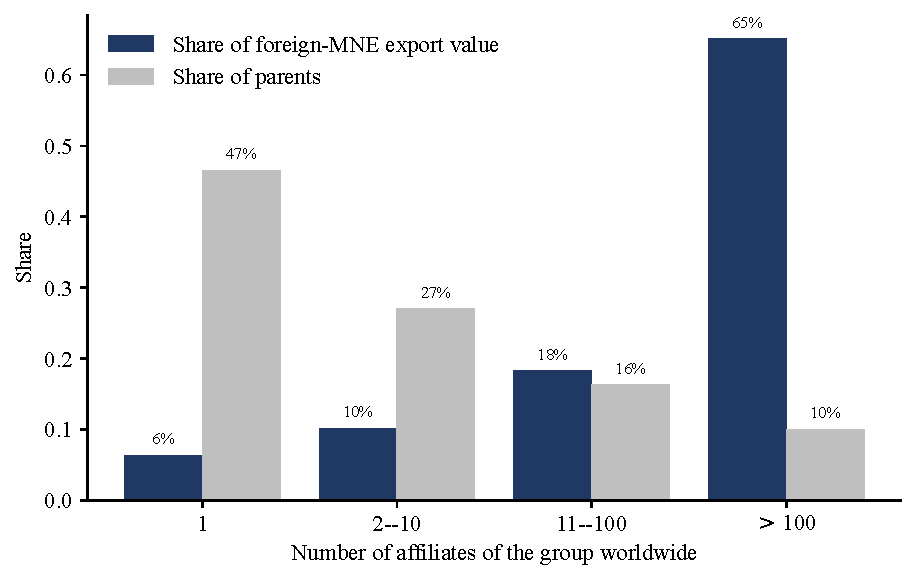
\includegraphics[width=0.7\textwidth,height=0.8\textheight,keepaspectratio]{figures/manufacturing/fig_wp0_fig5_network.pdf}%
  \caption{Manufacturing: Foreign-Multinational Exports and Number of Parents, by Size of the Group's Global Network}%
  \label{fig:net_manufacturing}%
  \par\vspace{2pt}%
  \parbox{0.92\textwidth}{\footnotesize %
  \textit{Notes:} Shares of foreign-MNE manufacturing export value and of parents, by the number of affiliates the group has worldwide.\\[3pt]%
  \textit{Source:} Authors' calculations based on customs data matched to Orbis and Dun \& Bradstreet.}%
  \end{figure}
% ---- Table: Manufacturing: Foreign-Multinational Exports and Number of Parents, by Size of the Group's Global Network
\begin{table}[H]\centering\small%
  \caption{Manufacturing: Foreign-Multinational Exports and Number of Parents, by Size of the Group's Global Network}%
  \label{tab:net_t_manufacturing}%
  \adjustbox{max width=\textwidth, max totalheight=0.8\textheight}{\begin{tabular}{lrrr}
\toprule
Affiliates worldwide & Parents & Share of parents (\%) & Share of foreign-MNE export value (\%) \\
\midrule
1 & 4,801 & 46.6 & 6.4 \\
2--10 & 2,787 & 27.0 & 10.2 \\
11--100 & 1,679 & 16.3 & 18.3 \\
$>$100 & 1,037 & 10.1 & 65.2 \\
\midrule
All parents & 10,304 & 100 & 100 \\
\bottomrule
\end{tabular}
}%
  \par\vspace{3pt}%
  \begin{minipage}{0.95\textwidth}\footnotesize %
  \textit{Notes:} Number and share of parents, and share of foreign-MNE manufacturing export value, by the number of affiliates the group has worldwide.\\[3pt]%
  \textit{Source:} Authors' calculations based on customs data matched to Orbis and Dun \& Bradstreet.%
  \end{minipage}%
  \end{table}

\subsection{Concentration within Products}
% ---- Figure: Manufacturing: Export Concentration within Products: Firms and Groups
\begin{figure}[H]\centering%
  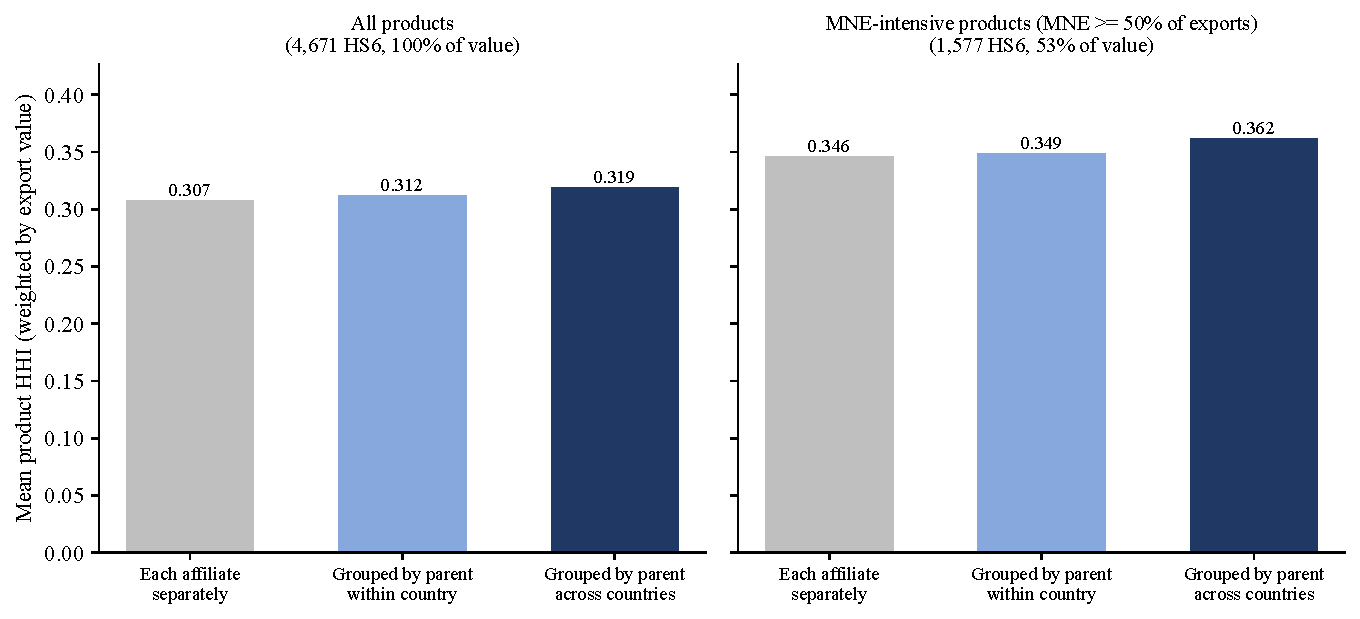
\includegraphics[width=0.9\textwidth,height=0.8\textheight,keepaspectratio]{figures/manufacturing/fig_wp0_fig6_hhi.pdf}%
  \caption{Manufacturing: Export Concentration within Products: Firms and Groups}%
  \label{fig:hhi_manufacturing}%
  \par\vspace{2pt}%
  \parbox{0.92\textwidth}{\footnotesize %
  \textit{Notes:} Mean Herfindahl index of exporters within each HS6 product, weighted by export value, counting each affiliate separately or grouping affiliates by parent within or across countries. Right panel: products where MNEs account for at least half of exports.\\[3pt]%
  \textit{Source:} Authors' calculations based on customs data matched to Orbis and Dun \& Bradstreet.}%
  \end{figure}
% ---- Table: Manufacturing: Export Concentration within Products: Firms and Groups
\begin{table}[H]\centering\small%
  \caption{Manufacturing: Export Concentration within Products: Firms and Groups}%
  \label{tab:hhi_t_manufacturing}%
  \adjustbox{max width=\textwidth, max totalheight=0.8\textheight}{\begin{tabular}{llrrr}
\toprule
Sample & Measure & Firm level & Groups within country & Groups across countries \\
\midrule
\multicolumn{5}{l}{\textit{All products: 4,671 HS6, 100\% of value}} \\
 & Mean HHI & 0.307 & 0.312 & 0.319 \\
 & Mean top-exporter share & 44.3\% & 44.4\% & 45.3\% \\
 & Effective number of exporters (1/HHI) & 7.5 & 7.2 & 6.9 \\
\multicolumn{5}{l}{\textit{MNE-intensive products (MNE $\geq$ 50\% of exports): 1,577 HS6, 53\% of value}} \\
 & Mean HHI & 0.346 & 0.349 & 0.362 \\
 & Mean top-exporter share & 46.8\% & 47.1\% & 48.7\% \\
 & Effective number of exporters (1/HHI) & 6.8 & 6.6 & 6.0 \\
\bottomrule
\end{tabular}
}%
  \par\vspace{3pt}%
  \begin{minipage}{0.95\textwidth}\footnotesize %
  \textit{Notes:} Means across HS6 products, weighted by export value. Firm level: each affiliate counted separately. Groups: affiliates grouped by ultimate parent within each exporting country or across countries.\\[3pt]%
  \textit{Source:} Authors' calculations based on customs data matched to Orbis and Dun \& Bradstreet.%
  \end{minipage}%
  \end{table}

\subsection{Groups and Affiliates}
% ---- Table: Manufacturing: Multinational Affiliates and Groups in Origin--Destination--Product--Year Cells
\begin{table}[H]\centering\small%
  \caption{Manufacturing: Multinational Affiliates and Groups in Origin--Destination--Product--Year Cells}%
  \label{tab:grp_manufacturing}%
  \adjustbox{max width=\textwidth, max totalheight=0.8\textheight}{\begin{tabular}{lr}
\toprule
Origin-destination-product-year cells with $\geq 1$ MNE & \\
\midrule
Cells & 834,508 \\
MNE affiliates per cell (mean) & 1.86 \\
MNE groups per cell (mean) & 1.85 \\
Affiliates per group, pooled & 1.00 \\
Affiliates per group, mean weighted by export value & 1.08 \\
Cells where one group exports through $>1$ affiliate (\%) & 0.7 \\
\bottomrule
\end{tabular}
}%
  \par\vspace{3pt}%
  \begin{minipage}{0.95\textwidth}\footnotesize %
  \textit{Notes:} Cells with at least one MNE. Group: ultimate parent in Orbis or Dun \& Bradstreet (parent name when the identifier is missing).\\[3pt]%
  \textit{Source:} Authors' calculations based on customs data matched to Orbis and Dun \& Bradstreet.%
  \end{minipage}%
  \end{table}
% ---- Table: Manufacturing: Multinational Presence and Exports: Affiliates and Groups
\begin{table}[H]\centering\small%
  \caption{Manufacturing: Multinational Presence and Exports: Affiliates and Groups}%
  \label{tab:grp_r_manufacturing}%
  \adjustbox{max width=\textwidth, max totalheight=0.8\textheight}{\begin{tabular}{lcccccc} \hline
 & \multicolumn{3}{c}{Origin $\times$ year, destination $\times$ year, product FE} & \multicolumn{3}{c}{Origin $\times$ dest. $\times$ product, origin $\times$ dest. $\times$ year FE} \\
 & (1) & (2) & (3) & (4) & (5) & (6) \\ \hline
\multicolumn{7}{l}{\textit{Panel A. Dependent variable: $\ln$ exports, all firms}} \\
$\ln$(\# MNE firms) & 2.0010*** &  &  & 0.9522*** &  &  \\
 & (0.0414) &  &  & (0.0238) &  &  \\
$\ln$(\# MNE groups) &  & 2.0024*** & 1.9951*** &  & 0.9521*** & 0.9526*** \\
 &  & (0.0413) & (0.0409) &  & (0.0240) & (0.0240) \\
$\ln$(affiliates per group) &  &  & 2.9370*** &  &  & 0.8982*** \\
 &  &  & (0.4047) &  &  & (0.0892) \\
\midrule
\multicolumn{7}{l}{\textit{Panel B. Dependent variable: $\ln$ exports, non-MNE firms}} \\
$\ln$(\# MNE firms) & 1.2489*** &  &  & 0.1925*** &  &  \\
 & (0.0367) &  &  & (0.0202) &  &  \\
$\ln$(\# MNE groups) &  & 1.2533*** & 1.2511*** &  & 0.1935*** & 0.1935*** \\
 &  & (0.0364) & (0.0361) &  & (0.0201) & (0.0201) \\
$\ln$(affiliates per group) &  &  & 0.8359 &  &  & -0.0193 \\
 &  &  & (0.5918) &  &  & (0.1346) \\
\hline
Product FE & $\checkmark$ & $\checkmark$ & $\checkmark$ &  &  &  \\
Origin $\times$ year FE & $\checkmark$ & $\checkmark$ & $\checkmark$ &  &  &  \\
Destination $\times$ year FE & $\checkmark$ & $\checkmark$ & $\checkmark$ &  &  &  \\
Origin $\times$ dest.\ $\times$ product FE &  &  &  & $\checkmark$ & $\checkmark$ & $\checkmark$ \\
Origin $\times$ dest.\ $\times$ year FE &  &  &  & $\checkmark$ & $\checkmark$ & $\checkmark$ \\
Observations (Panel A) & 834,033 & 834,033 & 834,033 & 726,525 & 726,525 & 726,525 \\
Observations (Panel B) & 375,761 & 375,761 & 375,761 & 338,556 & 338,556 & 338,556 \\
\hline
\end{tabular}
}%
  \par\vspace{3pt}%
  \begin{minipage}{0.95\textwidth}\footnotesize %
  \textit{Notes:} Observations are origin--destination--HS6--year cells. Manufacturing products only. Dependent variable: $\ln$ exports of the cell (Panel A) and of the non-MNE firms in the cell (Panel B). Regressors: $\ln$ number of MNE affiliates or $\ln$ number of MNE groups (distinct ultimate parents). Standard errors clustered by origin--destination pair in parentheses. *** $p<0.01$, ** $p<0.05$, * $p<0.1$.\\[3pt]%
  \textit{Source:} Authors' calculations based on customs data matched to Orbis and Dun \& Bradstreet.%
  \end{minipage}%
  \end{table}

\section{Fact 5: Multinational Presence Is Associated with Higher Exports}\label{sec:f5_manufacturing}
% ---- Table: Manufacturing: Multinational Presence and Exports
\begin{table}[H]\centering\small%
  \caption{Manufacturing: Multinational Presence and Exports}%
  \label{tab:t1_manufacturing}%
  \adjustbox{max width=\textwidth, max totalheight=0.8\textheight}{\begin{tabular}{lcccccc} \hline
 & \multicolumn{3}{c}{Intensive: $\ln$(\# MNE firms)} & \multicolumn{3}{c}{Extensive: any MNE present} \\
 & (1) & (2) & (3) & (1) & (2) & (3) \\ \hline
\multicolumn{7}{l}{\textit{Panel A. Dependent variable: $\ln$ exports, all firms}} \\
$\ln$(\# MNE firms) & 2.0181*** & 2.0010*** & 0.9522*** &  &  &  \\
 & (0.0409) & (0.0414) & (0.0238) &  &  &  \\
Any MNE present &  &  &  & 1.3806*** & 1.3800*** & 0.6850*** \\
 &  &  &  & (0.0397) & (0.0391) & (0.0182) \\
\midrule
\multicolumn{7}{l}{\textit{Panel B. Dependent variable: $\ln$ exports, non-MNE firms}} \\
$\ln$(\# MNE firms) & 1.2657*** & 1.2489*** & 0.1925*** &  &  &  \\
 & (0.0367) & (0.0367) & (0.0202) &  &  &  \\
Any MNE present &  &  &  & 1.2400*** & 1.2208*** & 0.0959*** \\
 &  &  &  & (0.0379) & (0.0372) & (0.0109) \\
\hline
Origin FE & $\checkmark$ &  &  & $\checkmark$ &  &  \\
Destination FE & $\checkmark$ &  &  & $\checkmark$ &  &  \\
Product FE & $\checkmark$ & $\checkmark$ &  & $\checkmark$ & $\checkmark$ &  \\
Year FE & $\checkmark$ &  &  & $\checkmark$ &  &  \\
Origin $\times$ year FE &  & $\checkmark$ &  &  & $\checkmark$ &  \\
Destination $\times$ year FE &  & $\checkmark$ &  &  & $\checkmark$ &  \\
Origin $\times$ dest.\ $\times$ product FE &  &  & $\checkmark$ &  &  & $\checkmark$ \\
Origin $\times$ dest.\ $\times$ year FE &  &  & $\checkmark$ &  &  & $\checkmark$ \\
Observations (Panel A) & 834,285 & 834,033 & 726,525 & 1,496,595 & 1,496,381 & 1,329,815 \\
Observations (Panel B) & 376,034 & 375,761 & 338,556 & 1,038,432 & 1,038,206 & 904,114 \\
\hline
\end{tabular}
}%
  \par\vspace{3pt}%
  \begin{minipage}{0.95\textwidth}\footnotesize %
  \textit{Notes:} Observations are origin--destination--HS6--year cells. Manufacturing products only. Dependent variable: $\ln$ exports of the cell (Panel A) and of the non-MNE firms in the cell (Panel B). Intensive margin: $\ln$ number of MNEs, cells with at least one MNE. Extensive margin: indicator for at least one MNE. Standard errors clustered by origin--destination pair in parentheses. *** $p<0.01$, ** $p<0.05$, * $p<0.1$.\\[3pt]%
  \textit{Source:} Authors' calculations based on customs data matched to Orbis and Dun \& Bradstreet.%
  \end{minipage}%
  \end{table}
% ---- Table: Manufacturing: Multinational Exports by Exporting Country and Destination Type
\begin{table}[H]\centering\small%
  \caption{Manufacturing: Multinational Exports by Exporting Country and Destination Type}%
  \label{tab:pres_manufacturing}%
  \adjustbox{max width=\textwidth, max totalheight=0.8\textheight}{\begin{tabular}{lrrrrr}
\toprule
Origin & MNE value (US\$bn/yr) & of which domestic (\%) & Foreign-MNE value (US\$bn/yr) & \multicolumn{2}{c}{\% of foreign-MNE value, by destination} \\
 & & & & parent country & other (of which: group affiliate there) \\
\midrule
ARG & 14.4 & 8.7 & 13.1 & 5.5 & 94.5 (55.3) \\
CHL & 8.7 & 26.6 & 6.4 & 4.1 & 95.9 (57.8) \\
COL & 5.9 & 12.9 & 5.2 & 4.0 & 96.0 (46.2) \\
CRI & 4.6 & 6.8 & 4.3 & 32.7 & 67.3 (28.0) \\
DOM & 3.4 & 0.9 & 3.4 & 25.3 & 74.7 (30.7) \\
PER & 2.8 & 12.5 & 2.5 & 5.0 & 95.0 (19.7) \\
PRY & 0.4 & 6.7 & 0.4 & 4.3 & 95.7 (45.2) \\
SLV & 2.0 & 0.7 & 2.0 & 47.4 & 52.6 (23.4) \\
URY & 1.6 & 16.5 & 1.3 & 9.6 & 90.4 (30.8) \\
\midrule
All & 43.9 & 13.4 & 38.5 & 11.9 & 88.1 (44.9) \\
\bottomrule
\end{tabular}
}%
  \par\vspace{3pt}%
  \begin{minipage}{0.95\textwidth}\footnotesize %
  \textit{Notes:} MNE and foreign-MNE manufacturing export value by country, and the split of foreign-MNE value by destination. Parent country: exports to the country of the ultimate parent. Other: all remaining destinations; in parentheses, destinations where the group has another affiliate. Values are annual averages in US\$ billion.\\[3pt]%
  \textit{Source:} Authors' calculations based on customs data matched to Orbis and Dun \& Bradstreet.%
  \end{minipage}%
  \end{table}
% ---- Table: Manufacturing: Multinational Presence and Exports: Intensive Margin, by Type of Multinational
\begin{table}[H]\centering\small%
  \caption{Manufacturing: Multinational Presence and Exports: Intensive Margin, by Type of Multinational}%
  \label{tab:cnt_manufacturing}%
  \adjustbox{max width=\textwidth, max totalheight=0.8\textheight}{\begin{tabular}{lcccccc} \hline
 & \multicolumn{2}{c}{All MNEs} & \multicolumn{2}{c}{Foreign / domestic} & \multicolumn{2}{c}{Foreign by destination, domestic} \\
 & (1) & (2) & (3) & (4) & (5) & (6) \\ \hline
\multicolumn{7}{l}{\textit{Panel A. Dependent variable: $\ln$ exports, all firms}} \\
$\ln$(\# MNE firms) & 2.0010*** & 0.9522*** &  &  &  &  \\
 & (0.0414) & (0.0238) &  &  &  &  \\
$\ln$(\# foreign MNEs) &  &  & 1.1644*** & 0.4435*** &  &  \\
 &  &  & (0.0358) & (0.0148) &  &  \\
$\ln$(\# foreign MNEs, parent-country destination) &  &  &  &  & 0.4294*** & 0.1248** \\
 &  &  &  &  & (0.1086) & (0.0474) \\
$\ln$(\# foreign MNEs, other destinations) &  &  &  &  & 0.9347*** & 0.3008*** \\
 &  &  &  &  & (0.0710) & (0.0431) \\
$\ln$(\# domestic MNEs) &  &  & 0.3833*** & 0.1904*** & 0.3269*** & 0.1636*** \\
 &  &  & (0.0319) & (0.0175) & (0.0729) & (0.0401) \\
\midrule
\multicolumn{7}{l}{\textit{Panel B. Dependent variable: $\ln$ exports, non-MNE firms}} \\
$\ln$(\# MNE firms) & 1.2489*** & 0.1925*** &  &  &  &  \\
 & (0.0367) & (0.0202) &  &  &  &  \\
$\ln$(\# foreign MNEs) &  &  & 1.0546*** & 0.1865*** &  &  \\
 &  &  & (0.0493) & (0.0250) &  &  \\
$\ln$(\# foreign MNEs, parent-country destination) &  &  &  &  & 0.2820** & 0.1364** \\
 &  &  &  &  & (0.1140) & (0.0611) \\
$\ln$(\# foreign MNEs, other destinations) &  &  &  &  & 0.9954*** & 0.1594** \\
 &  &  &  &  & (0.0680) & (0.0641) \\
$\ln$(\# domestic MNEs) &  &  & 0.4194*** & 0.0742*** & 0.3667*** & 0.1106** \\
 &  &  & (0.0419) & (0.0238) & (0.0885) & (0.0440) \\
\hline
Product FE & $\checkmark$ &  & $\checkmark$ &  & $\checkmark$ &  \\
Origin $\times$ year FE & $\checkmark$ &  & $\checkmark$ &  & $\checkmark$ &  \\
Destination $\times$ year FE & $\checkmark$ &  & $\checkmark$ &  & $\checkmark$ &  \\
Origin $\times$ dest.\ $\times$ product FE &  & $\checkmark$ &  & $\checkmark$ &  & $\checkmark$ \\
Origin $\times$ dest.\ $\times$ year FE &  & $\checkmark$ &  & $\checkmark$ &  & $\checkmark$ \\
Observations (Panel A) & 834,033 & 726,525 & 85,453 & 73,318 & 6,936 & 5,563 \\
Observations (Panel B) & 375,761 & 338,556 & 68,534 & 59,772 & 6,579 & 5,352 \\
\hline
\end{tabular}
}%
  \par\vspace{3pt}%
  \begin{minipage}{0.95\textwidth}\footnotesize %
  \textit{Notes:} Observations are origin--destination--HS6--year cells. Manufacturing products only. Dependent variable: $\ln$ exports of the cell (Panel A) and of the non-MNE firms in the cell (Panel B). Regressors: $\ln$ number of MNEs of each type. Columns (5)--(6) split foreign MNEs by whether the destination is the parent's country. Standard errors clustered by origin--destination pair in parentheses. *** $p<0.01$, ** $p<0.05$, * $p<0.1$.\\[3pt]%
  \textit{Source:} Authors' calculations based on customs data matched to Orbis and Dun \& Bradstreet.%
  \end{minipage}%
  \end{table}
% ---- Table: Manufacturing: Multinational Presence and Exports: Extensive Margin, by Type of Multinational
\begin{table}[H]\centering\small%
  \caption{Manufacturing: Multinational Presence and Exports: Extensive Margin, by Type of Multinational}%
  \label{tab:ext_manufacturing}%
  \adjustbox{max width=\textwidth, max totalheight=0.8\textheight}{\begin{tabular}{lcccccc} \hline
 & \multicolumn{2}{c}{All MNEs} & \multicolumn{2}{c}{Foreign / domestic} & \multicolumn{2}{c}{Foreign by destination, domestic} \\
 & (1) & (2) & (3) & (4) & (5) & (6) \\ \hline
\multicolumn{7}{l}{\textit{Panel A. Dependent variable: $\ln$ exports, all firms}} \\
Any MNE present & 1.3800*** & 0.6850*** &  &  &  &  \\
 & (0.0391) & (0.0182) &  &  &  &  \\
Any foreign MNE &  &  & 1.4231*** & 0.7021*** &  &  \\
 &  &  & (0.0344) & (0.0178) &  &  \\
Any foreign MNE, parent-country destination &  &  &  &  & 1.3645*** & 0.5991*** \\
 &  &  &  &  & (0.1114) & (0.0488) \\
Any foreign MNE, other destination &  &  &  &  & 1.4329*** & 0.7010*** \\
 &  &  &  &  & (0.0324) & (0.0164) \\
Any domestic MNE &  &  & 1.3878*** & 0.4684*** & 1.3589*** & 0.4682*** \\
 &  &  & (0.0466) & (0.0186) & (0.0440) & (0.0186) \\
\midrule
\multicolumn{7}{l}{\textit{Panel B. Dependent variable: $\ln$ exports, non-MNE firms}} \\
Any MNE present & 1.2208*** & 0.0959*** &  &  &  &  \\
 & (0.0372) & (0.0109) &  &  &  &  \\
Any foreign MNE &  &  & 1.1402*** & 0.0997*** &  &  \\
 &  &  & (0.0344) & (0.0114) &  &  \\
Any foreign MNE, parent-country destination &  &  &  &  & 0.9721*** & 0.1045*** \\
 &  &  &  &  & (0.1138) & (0.0202) \\
Any foreign MNE, other destination &  &  &  &  & 1.1200*** & 0.1030*** \\
 &  &  &  &  & (0.0329) & (0.0115) \\
Any domestic MNE &  &  & 1.0491*** & 0.0984*** & 1.0171*** & 0.0983*** \\
 &  &  & (0.0490) & (0.0167) & (0.0467) & (0.0167) \\
\hline
Product FE & $\checkmark$ &  & $\checkmark$ &  & $\checkmark$ &  \\
Origin $\times$ year FE & $\checkmark$ &  & $\checkmark$ &  & $\checkmark$ &  \\
Destination $\times$ year FE & $\checkmark$ &  & $\checkmark$ &  & $\checkmark$ &  \\
Origin $\times$ dest.\ $\times$ product FE &  & $\checkmark$ &  & $\checkmark$ &  & $\checkmark$ \\
Origin $\times$ dest.\ $\times$ year FE &  & $\checkmark$ &  & $\checkmark$ &  & $\checkmark$ \\
Observations (Panel A) & 1,496,381 & 1,329,815 & 1,496,381 & 1,329,815 & 1,496,381 & 1,329,815 \\
Observations (Panel B) & 1,038,206 & 904,114 & 1,038,206 & 904,114 & 1,038,206 & 904,114 \\
\hline
\end{tabular}
}%
  \par\vspace{3pt}%
  \begin{minipage}{0.95\textwidth}\footnotesize %
  \textit{Notes:} Observations are origin--destination--HS6--year cells. Manufacturing products only. Dependent variable: $\ln$ exports of the cell (Panel A) and of the non-MNE firms in the cell (Panel B). Regressors: indicators for at least one MNE of each type. Columns (5)--(6) split foreign MNEs by whether the destination is the parent's country. Standard errors clustered by origin--destination pair in parentheses. *** $p<0.01$, ** $p<0.05$, * $p<0.1$.\\[3pt]%
  \textit{Source:} Authors' calculations based on customs data matched to Orbis and Dun \& Bradstreet.%
  \end{minipage}%
  \end{table}

\section{Fact 6: Distance Is a Weaker Barrier for Multinationals}\label{sec:f6_manufacturing}
% ---- Table: Manufacturing: Distance and Firm Exports: Multinationals by Presence at the Destination
\begin{table}[H]\centering\small%
  \caption{Manufacturing: Distance and Firm Exports: Multinationals by Presence at the Destination}%
  \label{tab:t2_manufacturing}%
  \adjustbox{max width=\textwidth, max totalheight=0.8\textheight}{\begin{tabular}{lcccc} \hline
Dep.\ var.: $\ln$ exports & (1) & (2) & (3) & (4) \\ \hline
$\ln$ distance & -0.1509*** & -0.1741*** & -0.1499*** & -0.1730*** \\
 & (0.0454) & (0.0460) & (0.0453) & (0.0458) \\
$\ln$ distance $\times$ MNE & 0.0499*** & 0.0496*** &  &  \\
 & (0.0045) & (0.0045) &  &  \\
$\ln$ distance $\times$ MNE, present at destination &  &  & 0.0659*** & 0.0653*** \\
 &  &  & (0.0081) & (0.0081) \\
$\ln$ distance $\times$ MNE, not present at destination &  &  & 0.0444*** & 0.0443*** \\
 &  &  & (0.0037) & (0.0037) \\
\hline
Origin FE & $\checkmark$ &  & $\checkmark$ &  \\
Destination FE & $\checkmark$ &  & $\checkmark$ &  \\
Year FE & $\checkmark$ &  & $\checkmark$ &  \\
Origin $\times$ year FE &  & $\checkmark$ &  & $\checkmark$ \\
Destination $\times$ year FE &  & $\checkmark$ &  & $\checkmark$ \\
Product FE & $\checkmark$ & $\checkmark$ & $\checkmark$ & $\checkmark$ \\
\hline
Observations & 3,917,960 & 3,917,765 & 3,917,960 & 3,917,765 \\
\hline
\end{tabular}
}%
  \par\vspace{3pt}%
  \begin{minipage}{0.95\textwidth}\footnotesize %
  \textit{Notes:} Observations are firm--destination--HS6--year cells. Manufacturing products only. Dependent variable: $\ln$ exports. Non-MNE firms are the omitted group. Present: the group has an affiliate in the destination or the destination is the parent's country. Standard errors clustered by origin--destination pair in parentheses. *** $p<0.01$, ** $p<0.05$, * $p<0.1$.\\[3pt]%
  \textit{Source:} Authors' calculations based on customs data matched to Orbis and Dun \& Bradstreet.%
  \end{minipage}%
  \end{table}
% ---- Table: Manufacturing: Distance and Firm Exports: Foreign and Domestic Multinationals
\begin{table}[H]\centering\small%
  \caption{Manufacturing: Distance and Firm Exports: Foreign and Domestic Multinationals}%
  \label{tab:dist_manufacturing}%
  \adjustbox{max width=\textwidth, max totalheight=0.8\textheight}{\begin{tabular}{lcccc} \hline
Dep.\ var.: $\ln$ exports & (1) & (2) & (3) & (4) \\ \hline
$\ln$ distance & -0.1510*** & -0.1742*** & -0.1507*** & -0.1738*** \\
 & (0.0454) & (0.0459) & (0.0455) & (0.0460) \\
$\ln$ distance $\times$ foreign MNE & 0.0515*** & 0.0512*** &  &  \\
 & (0.0048) & (0.0048) &  &  \\
$\ln$ distance $\times$ foreign MNE, parent-country destination &  &  & 0.0690*** & 0.0687*** \\
 &  &  & (0.0189) & (0.0193) \\
$\ln$ distance $\times$ foreign MNE, other destination &  &  & 0.0502*** & 0.0498*** \\
 &  &  & (0.0041) & (0.0040) \\
$\ln$ distance $\times$ domestic MNE & 0.0388*** & 0.0390*** & 0.0386*** & 0.0388*** \\
 & (0.0052) & (0.0052) & (0.0051) & (0.0051) \\
\hline
Origin FE & $\checkmark$ &  & $\checkmark$ &  \\
Destination FE & $\checkmark$ &  & $\checkmark$ &  \\
Year FE & $\checkmark$ &  & $\checkmark$ &  \\
Origin $\times$ year FE &  & $\checkmark$ &  & $\checkmark$ \\
Destination $\times$ year FE &  & $\checkmark$ &  & $\checkmark$ \\
Product FE & $\checkmark$ & $\checkmark$ & $\checkmark$ & $\checkmark$ \\
\hline
Observations & 3,917,960 & 3,917,765 & 3,917,960 & 3,917,765 \\
\hline
\end{tabular}
}%
  \par\vspace{3pt}%
  \begin{minipage}{0.95\textwidth}\footnotesize %
  \textit{Notes:} Observations are firm--destination--HS6--year cells. Manufacturing products only. Dependent variable: $\ln$ exports. Non-MNE firms are the omitted group. Columns (3)--(4) split foreign MNEs by whether the destination is the parent's country. Standard errors clustered by origin--destination pair in parentheses. *** $p<0.01$, ** $p<0.05$, * $p<0.1$.\\[3pt]%
  \textit{Source:} Authors' calculations based on customs data matched to Orbis and Dun \& Bradstreet.%
  \end{minipage}%
  \end{table}

\section{Products}\label{sec:hs6_manufacturing}
% ---- Figure: Manufacturing: Ownership of the Twenty Largest Export Products
\begin{figure}[H]\centering%
  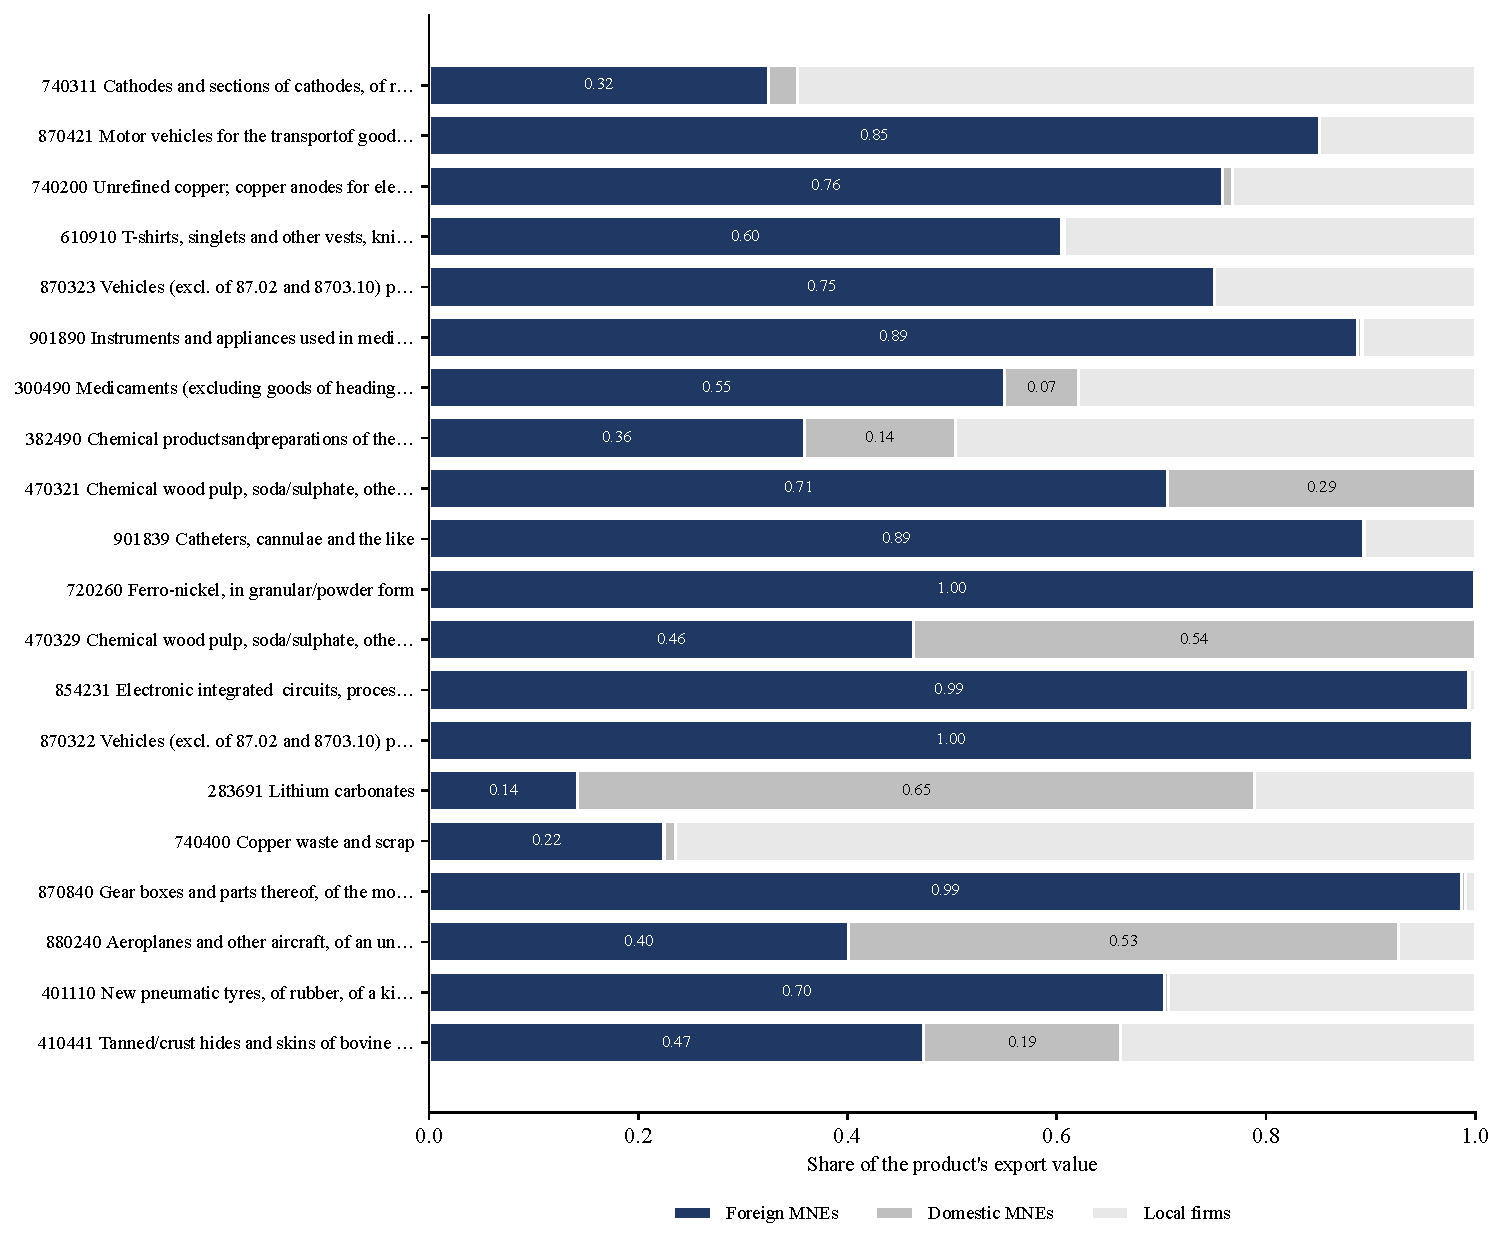
\includegraphics[width=1.0\textwidth,height=0.8\textheight,keepaspectratio]{figures/manufacturing/fig_wp1f_top20_hs6_stacked.pdf}%
  \caption{Manufacturing: Ownership of the Twenty Largest Export Products}%
  \label{fig:hs_st_manufacturing}%
  \par\vspace{2pt}%
  \parbox{0.92\textwidth}{\footnotesize %
  \textit{Notes:} Shares of each product's export value. Twenty largest HS6 products by export value.\\[3pt]%
  \textit{Source:} Authors' calculations based on customs data matched to Orbis and Dun \& Bradstreet.}%
  \end{figure}
% ---- Figure: Manufacturing: Ownership of the Twenty Largest Export Products, by Parent Country
\begin{figure}[H]\centering%
  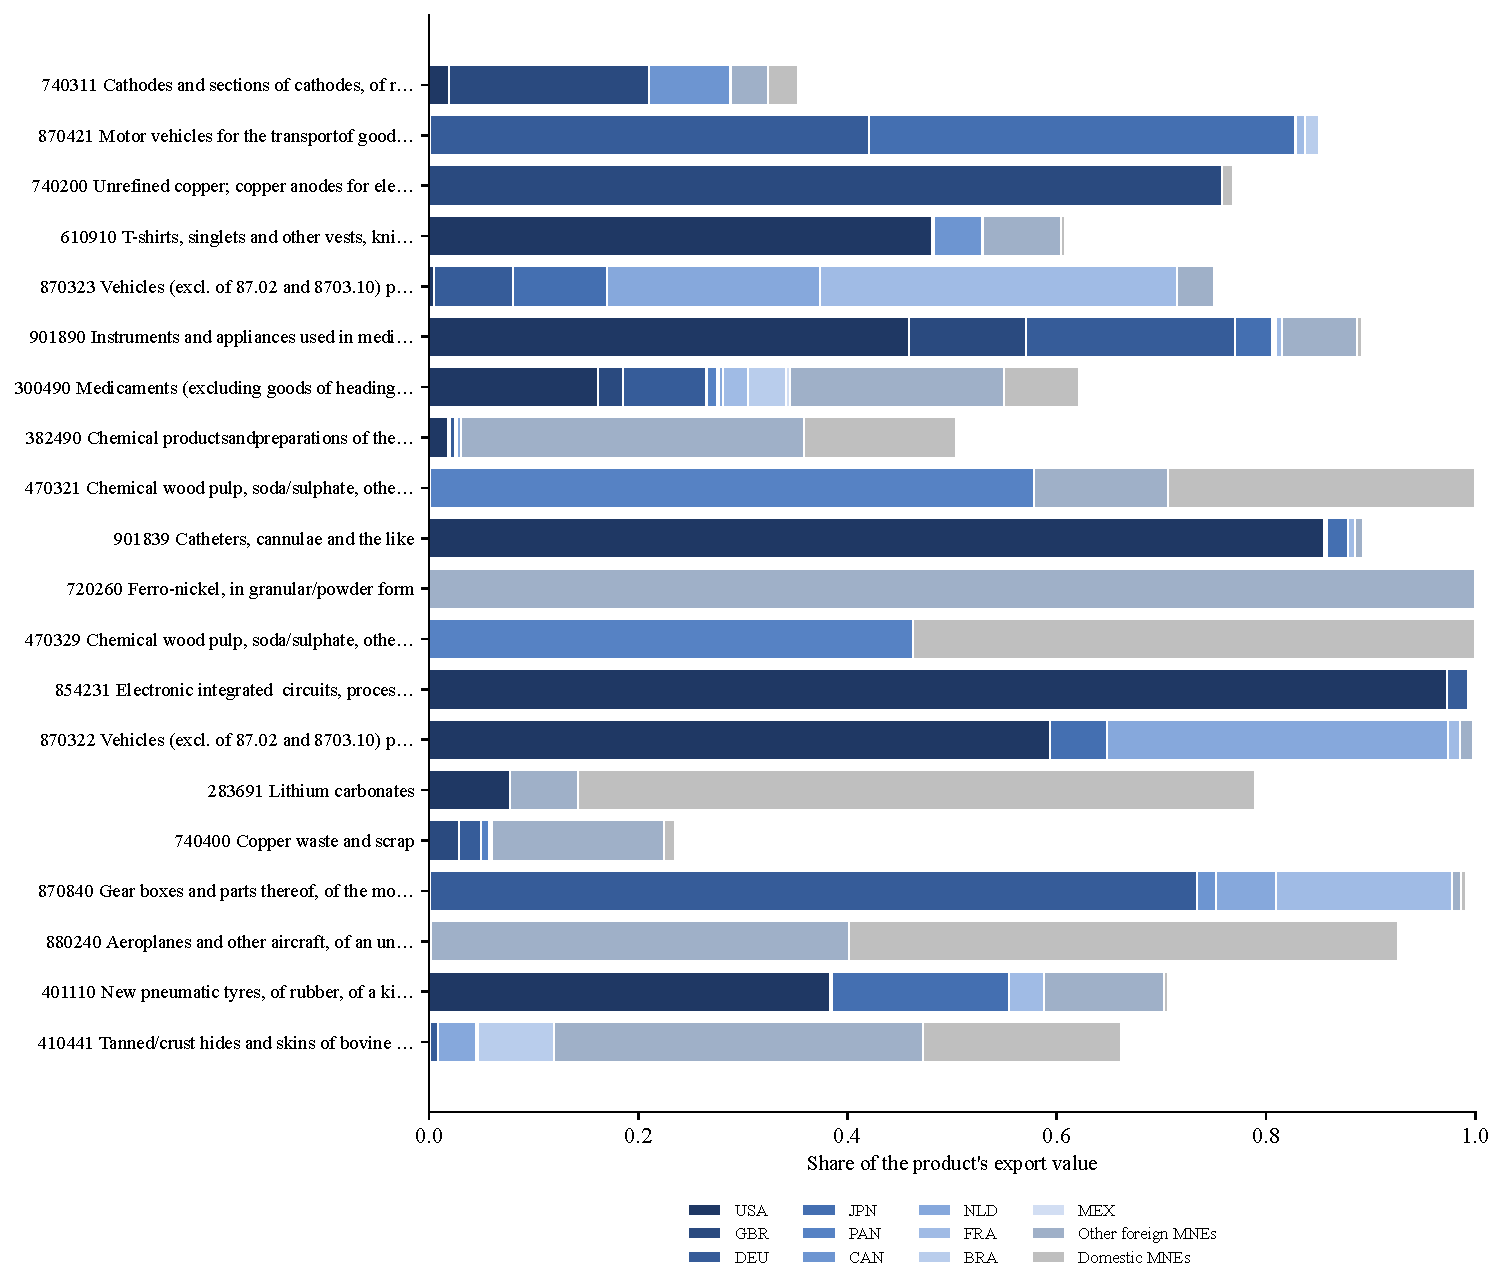
\includegraphics[width=1.0\textwidth,height=0.8\textheight,keepaspectratio]{figures/manufacturing/fig_wp1f_top20_hs6_by_parent.pdf}%
  \caption{Manufacturing: Ownership of the Twenty Largest Export Products, by Parent Country}%
  \label{fig:hs_par_manufacturing}%
  \par\vspace{2pt}%
  \parbox{0.92\textwidth}{\footnotesize %
  \textit{Notes:} Shares of each product's export value. Foreign-MNE share split by country of the ultimate parent; the unfilled part of each bar is local firms.\\[3pt]%
  \textit{Source:} Authors' calculations based on customs data matched to Orbis and Dun \& Bradstreet.}%
  \end{figure}
% ---- Figure: Manufacturing: Distribution of Export Value by Product-Level Foreign-Multinational Share
\begin{figure}[H]\centering%
  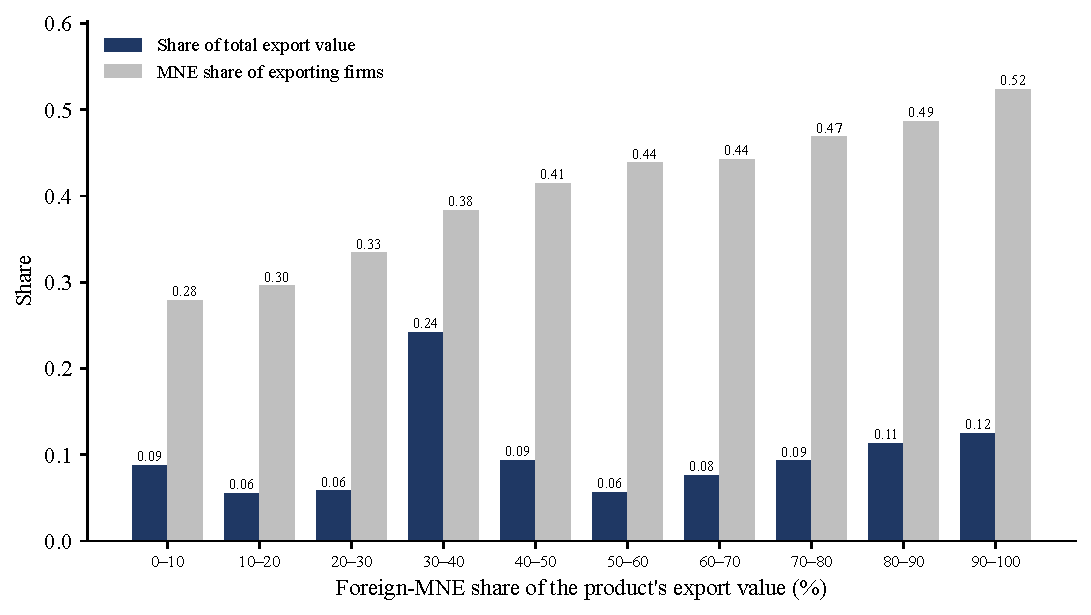
\includegraphics[width=0.85\textwidth,height=0.8\textheight,keepaspectratio]{figures/manufacturing/fig_wp1f_foreign_share_distribution.pdf}%
  \caption{Manufacturing: Distribution of Export Value by Product-Level Foreign-Multinational Share}%
  \label{fig:hs_dist_manufacturing}%
  \par\vspace{2pt}%
  \parbox{0.92\textwidth}{\footnotesize %
  \textit{Notes:} Share of manufacturing export value and MNE share of exporting firms, by the foreign-MNE share of each HS6 product's export value.\\[3pt]%
  \textit{Source:} Authors' calculations based on customs data matched to Orbis and Dun \& Bradstreet.}%
  \end{figure}
% ---- Table: Manufacturing: Distribution of Export Value by Product-Level Foreign-Multinational Share
\begin{table}[H]\centering\small%
  \caption{Manufacturing: Distribution of Export Value by Product-Level Foreign-Multinational Share}%
  \label{tab:hs_dist_t_manufacturing}%
  \adjustbox{max width=\textwidth, max totalheight=0.8\textheight}{\begin{tabular}{lrrr}
\toprule
Foreign share bin (\%) & Share of value & MNE share of exporting firms & HS6 products \\
\midrule
0--10 & 0.088 & 0.279 & 1,005 \\
10--20 & 0.056 & 0.296 & 537 \\
20--30 & 0.058 & 0.334 & 489 \\
30--40 & 0.241 & 0.383 & 472 \\
40--50 & 0.094 & 0.415 & 451 \\
50--60 & 0.057 & 0.438 & 368 \\
60--70 & 0.076 & 0.442 & 323 \\
70--80 & 0.093 & 0.468 & 267 \\
80--90 & 0.113 & 0.486 & 275 \\
90--100 & 0.125 & 0.524 & 484 \\
\bottomrule
\end{tabular}
}%
  \par\vspace{3pt}%
  \begin{minipage}{0.95\textwidth}\footnotesize %
  \textit{Notes:} Share of manufacturing export value and MNE share of exporting firms, by the foreign-MNE share of each HS6 product's export value. MNE share of exporting firms: MNE firm--destination--product--year observations over all observations in the bin.\\[3pt]%
  \textit{Source:} Authors' calculations based on customs data matched to Orbis and Dun \& Bradstreet.%
  \end{minipage}%
  \end{table}
% ---- Figure: Manufacturing: Concentration of Exports across Products
\begin{figure}[H]\centering%
  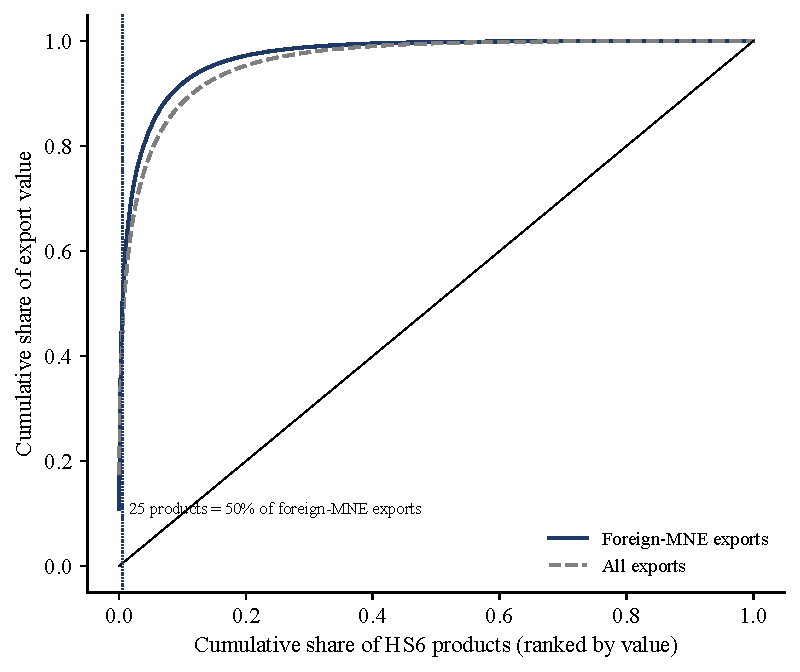
\includegraphics[width=0.6\textwidth,height=0.8\textheight,keepaspectratio]{figures/manufacturing/fig_wp1f_lorenz_foreign.pdf}%
  \caption{Manufacturing: Concentration of Exports across Products}%
  \label{fig:hs_lor_manufacturing}%
  \par\vspace{2pt}%
  \parbox{0.92\textwidth}{\footnotesize %
  \textit{Notes:} Cumulative share of export value against the cumulative share of HS6 products, ranked by value, for foreign-MNE exports and for all exports.\\[3pt]%
  \textit{Source:} Authors' calculations based on customs data matched to Orbis and Dun \& Bradstreet.}%
  \end{figure}
% ---- Table: Manufacturing: Exports and Multinational Shares, by HS Section
\begin{table}[H]\centering\footnotesize%
  \caption{Manufacturing: Exports and Multinational Shares, by HS Section}%
  \label{tab:hs_sec_manufacturing}%
  \adjustbox{max width=\textwidth, max totalheight=0.8\textheight}{\begin{tabular}{@{}p{7.2cm} r r r r l@{}}
\toprule
HS section & US\$bn/yr & Foreign (\%) & Domestic (\%) & Local (\%) & Leading parent \\
\midrule
XV Base metals & 19.6 & 41 & 3 & 56 & GBR (0.44) \\
VI Chemicals & 11.6 & 49 & 14 & 37 & USA (0.25) \\
XVII Transport equipment & 9.7 & 78 & 4 & 18 & DEU (0.30) \\
XI Textiles and apparel & 6.9 & 49 & 3 & 48 & USA (0.62) \\
XVI Machinery and electrical equipment & 6.2 & 63 & 4 & 33 & USA (0.41) \\
VII Plastics and rubber & 5.8 & 51 & 8 & 42 & USA (0.34) \\
X Pulp, paper & 3.4 & 54 & 28 & 18 & PAN (0.54) \\
XVIII Optical, precision instruments & 3.4 & 72 & 8 & 19 & USA (0.66) \\
IX Wood and articles & 1.9 & 27 & 34 & 39 & BHS (0.24) \\
VIII Hides, skins, leather & 1.6 & 40 & 12 & 49 & BGR (0.19) \\
XIII Stone, ceramics, glass & 0.9 & 49 & 4 & 46 & USA (0.32) \\
XX Miscellaneous manufactures & 0.9 & 53 & 7 & 40 & USA (0.48) \\
XII Footwear, headgear & 0.5 & 48 & 1 & 50 & USA (0.66) \\
XXI Works of art & 0.1 & 58 & 1 & 41 & BGR (0.94) \\
XIX Arms & 0.0 & 1 & 0 & 99 & CHE (0.82) \\
\midrule
All sections & 72.7 & 52 & 8 & 40 & \\
\bottomrule
\end{tabular}
}%
  \par\vspace{3pt}%
  \begin{minipage}{0.95\textwidth}\footnotesize %
  \textit{Notes:} Foreign, domestic and local: percent of each section's export value. Leading parent: largest parent country and its share of the section's foreign-MNE exports. Values are annual averages in US\$ billion.\\[3pt]%
  \textit{Source:} Authors' calculations based on customs data matched to Orbis and Dun \& Bradstreet.%
  \end{minipage}%
  \end{table}
% ---- Table: Manufacturing: Thirty Largest Export Products
\begin{table}[H]\centering\footnotesize%
  \caption{Manufacturing: Thirty Largest Export Products}%
  \label{tab:hs_by_value_manufacturing}%
  \adjustbox{max width=\textwidth, max totalheight=0.8\textheight}{\begin{tabular}{@{}l p{6.4cm} r r r r l@{}}
\toprule
HS6 & Description & US\$bn/yr & Foreign (\%) & Domestic (\%) & Local (\%) & Leading parent \\
\midrule
740311 & Cathodes and sections of cathodes, of refined copper, unwrought & 10.4 & 32 & 3 & 65 & GBR (0.59) \\
870421 & Motor vehicles for the transportof goods (excl. of 8704.10), with C-I internal combustion pist... & 3.2 & 85 & 0 & 15 & DEU (0.49) \\
740200 & Unrefined copper; copper anodes for electrolytic refining & 1.3 & 76 & 1 & 23 & GBR (1.00) \\
610910 & T-shirts, singlets and other vests, knitted/\allowbreak{}crocheted, of cotton & 1.3 & 60 & 0 & 39 & USA (0.79) \\
870323 & Vehicles (excl. of 87.02 and 8703.10) principally designed for the transportof persons, with s... & 1.3 & 75 & 0 & 25 & FRA (0.45) \\
901890 & Instruments and appliances used in medical/\allowbreak{}surgical/\allowbreak{}veterinary sciences, incl. other electro-m... & 1.4 & 89 & 0 & 11 & USA (0.52) \\
300490 & Medicaments (excluding goods of heading 30.02/\allowbreak{}30.05/\allowbreak{}30.06/\allowbreak{}3004.10-3004.50) consisting of mixed... & 1.0 & 55 & 7 & 38 & USA (0.29) \\
382490 & Chemical productsandpreparations of the chemical/\allowbreak{}allied industries (including those consisting... & 1.2 & 36 & 14 & 50 & LIE (0.61) \\
470321 & Chemical wood pulp, soda/\allowbreak{}sulphate, other than dissolving grades, semi-bleached/\allowbreak{}bleached, conif... & 0.7 & 71 & 29 & 0 & PAN (0.82) \\
901839 & Catheters, cannulae and the like & 0.9 & 89 & 0 & 11 & USA (0.96) \\
720260 & Ferro-nickel, in granular/\allowbreak{}powder form & 0.8 & 100 & 0 & 0 & ZAF (0.85) \\
470329 & Chemical wood pulp, soda/\allowbreak{}sulphate, other than dissolving grades, semi-bleached/\allowbreak{}bleached, non-c... & 0.6 & 46 & 54 & 0 & PAN (1.00) \\
854231 & Electronic integrated  circuits, processors and controllers, whether/\allowbreak{}not combined with memorie... & 0.8 & 99 & 0 & 1 & USA (0.98) \\
870322 & Vehicles (excl. of 87.02 and 8703.10) principally designed for the transportof persons, with s... & 0.8 & 100 & 0 & 0 & USA (0.59) \\
283691 & Lithium carbonates & 0.6 & 14 & 65 & 21 & USA (0.54) \\
740400 & Copper waste and scrap & 0.5 & 22 & 1 & 76 & BGR (0.39) \\
870840 & Gear boxes and parts thereof, of the motor vehicles of headings 87.01 to 87.05. & 0.6 & 99 & 0 & 1 & DEU (0.74) \\
880240 & Aeroplanes and other aircraft, of an unladen weight >15000kg & 0.6 & 40 & 53 & 7 & CHL (0.99) \\
401110 & New pneumatic tyres, of rubber, of a kind used on motor cars (incl. station wagons and racing ... & 0.5 & 70 & 0 & 29 & USA (0.55) \\
410441 & Tanned/\allowbreak{}crust hides and skins of bovine (incl. buffalo)/\allowbreak{}equine animals, without hair on, in the... & 0.5 & 47 & 19 & 34 & BGR (0.33) \\
730429 & Other casing, tubing, of a kind used in drilling for oil/\allowbreak{}gas (excld. of 7304.22/\allowbreak{}23/\allowbreak{}24), other ... & 0.5 & 4 & 0 & 96 & CHE (0.70) \\
392330 & Carboys, bottles, flasks and similar articles, of plastics & 0.5 & 46 & 26 & 28 & CAN (0.54) \\
870321 & Vehicles (excl. of 87.02 and 8703.10) principally designed for the transportof persons, with s... & 0.5 & 100 & 0 & 0 & NLD (0.49) \\
740811 & Copper wire, of refined copper of which the maximum cross-sectional dim. exceeds 6mm & 0.4 & 62 & 0 & 38 & USA (0.50) \\
800110 & Tin, not alloyed, unwrought & 0.4 & 0 & 0 & 100 & FRA (0.49) \\
390410 & Poly(vinyl chloride), not mixed with any other substance, in primary forms & 0.4 & 100 & 0 & 0 & MEX (0.83) \\
390210 & Polypropylene, in primary forms & 0.4 & 16 & 0 & 84 & ESP (0.55) \\
380892 & Fungicides, put up in forms/\allowbreak{}packings for retail sale/\allowbreak{}as preparations/\allowbreak{}articles  & 0.4 & 82 & 2 & 16 & USA (0.42) \\
280120 & Iodine & 0.3 & 8 & 17 & 76 & CAN (1.00) \\
902139 & Artificial parts of the body other than teeth, dental fittings and joints & 0.4 & 10 & 60 & 30 & VGB (0.46) \\
\bottomrule
\end{tabular}
}%
  \par\vspace{3pt}%
  \begin{minipage}{0.95\textwidth}\footnotesize %
  \textit{Notes:} Thirty largest HS6 products by export value. Foreign, domestic and local: percent of the product's export value. Leading parent: largest parent country and its share of the product's foreign-MNE exports. Values are annual averages in US\$ billion.\\[3pt]%
  \textit{Source:} Authors' calculations based on customs data matched to Orbis and Dun \& Bradstreet.%
  \end{minipage}%
  \end{table}
% ---- Table: Manufacturing: Thirty Largest Export Products of Foreign Multinationals
\begin{table}[H]\centering\footnotesize%
  \caption{Manufacturing: Thirty Largest Export Products of Foreign Multinationals}%
  \label{tab:hs_by_foreign_value_manufacturing}%
  \adjustbox{max width=\textwidth, max totalheight=0.8\textheight}{\begin{tabular}{@{}l p{6.4cm} r r r r l@{}}
\toprule
HS6 & Description & US\$bn/yr & Foreign (\%) & Domestic (\%) & Local (\%) & Leading parent \\
\midrule
740311 & Cathodes and sections of cathodes, of refined copper, unwrought & 10.4 & 32 & 3 & 65 & GBR (0.59) \\
870421 & Motor vehicles for the transportof goods (excl. of 8704.10), with C-I internal combustion pist... & 3.2 & 85 & 0 & 15 & DEU (0.49) \\
740200 & Unrefined copper; copper anodes for electrolytic refining & 1.3 & 76 & 1 & 23 & GBR (1.00) \\
901890 & Instruments and appliances used in medical/\allowbreak{}surgical/\allowbreak{}veterinary sciences, incl. other electro-m... & 1.4 & 89 & 0 & 11 & USA (0.52) \\
870323 & Vehicles (excl. of 87.02 and 8703.10) principally designed for the transportof persons, with s... & 1.3 & 75 & 0 & 25 & FRA (0.45) \\
610910 & T-shirts, singlets and other vests, knitted/\allowbreak{}crocheted, of cotton & 1.3 & 60 & 0 & 39 & USA (0.79) \\
720260 & Ferro-nickel, in granular/\allowbreak{}powder form & 0.8 & 100 & 0 & 0 & ZAF (0.85) \\
901839 & Catheters, cannulae and the like & 0.9 & 89 & 0 & 11 & USA (0.96) \\
854231 & Electronic integrated  circuits, processors and controllers, whether/\allowbreak{}not combined with memorie... & 0.8 & 99 & 0 & 1 & USA (0.98) \\
870322 & Vehicles (excl. of 87.02 and 8703.10) principally designed for the transportof persons, with s... & 0.8 & 100 & 0 & 0 & USA (0.59) \\
470321 & Chemical wood pulp, soda/\allowbreak{}sulphate, other than dissolving grades, semi-bleached/\allowbreak{}bleached, conif... & 0.7 & 71 & 29 & 0 & PAN (0.82) \\
300490 & Medicaments (excluding goods of heading 30.02/\allowbreak{}30.05/\allowbreak{}30.06/\allowbreak{}3004.10-3004.50) consisting of mixed... & 1.0 & 55 & 7 & 38 & USA (0.29) \\
870840 & Gear boxes and parts thereof, of the motor vehicles of headings 87.01 to 87.05. & 0.6 & 99 & 0 & 1 & DEU (0.74) \\
870321 & Vehicles (excl. of 87.02 and 8703.10) principally designed for the transportof persons, with s... & 0.5 & 100 & 0 & 0 & NLD (0.49) \\
390410 & Poly(vinyl chloride), not mixed with any other substance, in primary forms & 0.4 & 100 & 0 & 0 & MEX (0.83) \\
382490 & Chemical productsandpreparations of the chemical/\allowbreak{}allied industries (including those consisting... & 1.2 & 36 & 14 & 50 & LIE (0.61) \\
470329 & Chemical wood pulp, soda/\allowbreak{}sulphate, other than dissolving grades, semi-bleached/\allowbreak{}bleached, non-c... & 0.6 & 46 & 54 & 0 & PAN (1.00) \\
853620 & Automatic circuit breakers, for a voltage not >1000V & 0.4 & 99 & 0 & 1 & IRL (0.89) \\
401110 & New pneumatic tyres, of rubber, of a kind used on motor cars (incl. station wagons and racing ... & 0.5 & 70 & 0 & 29 & USA (0.55) \\
870333 & Vehicles principally designed for the transportof persons (excl. of 87.02 and 8703.10-8703.24)... & 0.4 & 100 & 0 & 0 & JPN (1.00) \\
380892 & Fungicides, put up in forms/\allowbreak{}packings for retail sale/\allowbreak{}as preparations/\allowbreak{}articles  & 0.4 & 82 & 2 & 16 & USA (0.42) \\
790111 & Zinc, not alloyed, unwrought, containing by weight 99.99\%/\allowbreak{}more of zinc & 0.3 & 97 & 0 & 3 & BRA (0.90) \\
740811 & Copper wire, of refined copper of which the maximum cross-sectional dim. exceeds 6mm & 0.4 & 62 & 0 & 38 & USA (0.50) \\
380891 & Insecticides, put up in forms/\allowbreak{}packings for retail sale/\allowbreak{}as preparations/\allowbreak{}articles  & 0.3 & 77 & 4 & 18 & DEU (0.52) \\
410441 & Tanned/\allowbreak{}crust hides and skins of bovine (incl. buffalo)/\allowbreak{}equine animals, without hair on, in the... & 0.5 & 47 & 19 & 34 & BGR (0.33) \\
961900 & Sanitary towels and tampons, napkins and napkin liners for babies and similar sanitary article... & 0.2 & 97 & 1 & 1 & USA (0.79) \\
790112 & Zinc, not alloyed, unwrought, containing by weight <99.99\% of zinc & 0.2 & 100 & 0 & 0 & BRA (1.00) \\
392330 & Carboys, bottles, flasks and similar articles, of plastics & 0.5 & 46 & 26 & 28 & CAN (0.54) \\
854430 & Ignition wiring sets and other wiring sets of a kind used in vehicles/\allowbreak{}aircraft/\allowbreak{}ships & 0.2 & 98 & 0 & 2 & JPN (0.81) \\
880240 & Aeroplanes and other aircraft, of an unladen weight >15000kg & 0.6 & 40 & 53 & 7 & CHL (0.99) \\
\bottomrule
\end{tabular}
}%
  \par\vspace{3pt}%
  \begin{minipage}{0.95\textwidth}\footnotesize %
  \textit{Notes:} Thirty largest HS6 products by foreign-MNE export value. Foreign, domestic and local: percent of the product's export value. Leading parent: largest parent country and its share of the product's foreign-MNE exports. Values are annual averages in US\$ billion.\\[3pt]%
  \textit{Source:} Authors' calculations based on customs data matched to Orbis and Dun \& Bradstreet.%
  \end{minipage}%
  \end{table}
% ---- Table: Manufacturing: Products with the Highest Foreign-Multinational Share
\begin{table}[H]\centering\footnotesize%
  \caption{Manufacturing: Products with the Highest Foreign-Multinational Share}%
  \label{tab:hs_by_foreign_share_manufacturing}%
  \adjustbox{max width=\textwidth, max totalheight=0.8\textheight}{\begin{tabular}{@{}l p{6.4cm} r r r r l@{}}
\toprule
HS6 & Description & US\$bn/yr & Foreign (\%) & Domestic (\%) & Local (\%) & Leading parent \\
\midrule
720260 & Ferro-nickel, in granular/\allowbreak{}powder form & 0.76 & 100 & 0 & 0 & ZAF (0.85) \\
790500 & Zinc plates, sheets, strip and foil & 0.05 & 100 & 0 & 0 & GBR (0.94) \\
790112 & Zinc, not alloyed, unwrought, containing by weight <99.99\% of zinc & 0.22 & 100 & 0 & 0 & BRA (1.00) \\
870321 & Vehicles (excl. of 87.02 and 8703.10) principally designed for the transportof persons, with s... & 0.53 & 100 & 0 & 0 & NLD (0.49) \\
390410 & Poly(vinyl chloride), not mixed with any other substance, in primary forms & 0.38 & 100 & 0 & 0 & MEX (0.83) \\
870322 & Vehicles (excl. of 87.02 and 8703.10) principally designed for the transportof persons, with s... & 0.82 & 100 & 0 & 0 & USA (0.59) \\
870333 & Vehicles principally designed for the transportof persons (excl. of 87.02 and 8703.10-8703.24)... & 0.39 & 100 & 0 & 0 & JPN (1.00) \\
280300 & Carbon (carbon blacks and other forms of carbon, n.e.s.) & 0.08 & 100 & 0 & 0 & USA (0.99) \\
470311 & Chemical wood pulp, soda/\allowbreak{}sulphate, other than dissolving grades, unbleached, coniferous & 0.14 & 100 & 0 & 0 & PAN (1.00) \\
300691 & Appliances identifiable for ostomy use & 0.19 & 100 & 0 & 0 & GBR (0.80) \\
853620 & Automatic circuit breakers, for a voltage not >1000V & 0.45 & 99 & 0 & 1 & IRL (0.89) \\
854231 & Electronic integrated  circuits, processors and controllers, whether/\allowbreak{}not combined with memorie... & 0.76 & 99 & 0 & 1 & USA (0.98) \\
381512 & Supported catalysts, with precious metal/\allowbreak{}precious metal comps. as the active substance & 0.08 & 99 & 0 & 1 & GBR (0.80) \\
870840 & Gear boxes and parts thereof, of the motor vehicles of headings 87.01 to 87.05. & 0.63 & 99 & 0 & 1 & DEU (0.74) \\
620711 & Men's/\allowbreak{}boys' underpants and briefs (excl. knitted/\allowbreak{}crocheted), of cotton & 0.05 & 98 & 0 & 2 & USA (1.00) \\
854430 & Ignition wiring sets and other wiring sets of a kind used in vehicles/\allowbreak{}aircraft/\allowbreak{}ships & 0.23 & 98 & 0 & 2 & JPN (0.81) \\
740710 & Bars, rods and profiles, of refined copper & 0.06 & 98 & 0 & 1 & MEX (0.73) \\
390120 & Polyethylene having a sp.gr. of 0.94/\allowbreak{}more, in primary forms & 0.13 & 98 & 0 & 2 & USA (0.98) \\
961900 & Sanitary towels and tampons, napkins and napkin liners for babies and similar sanitary article... & 0.22 & 97 & 1 & 1 & USA (0.79) \\
350300 & Gelatin, incl. gelatin in rectangular (incl. square) sheets, whether/\allowbreak{}not surface-worked /\allowbreak{}colou... & 0.08 & 97 & 0 & 3 & BEL (0.43) \\
790111 & Zinc, not alloyed, unwrought, containing by weight 99.99\%/\allowbreak{}more of zinc & 0.35 & 97 & 0 & 3 & BRA (0.90) \\
521213 & Woven fabrics of cotton (excl. of 52.08-52.11), dyed, weighing not >200 g/\allowbreak{}m2 & 0.13 & 96 & 0 & 4 & USA (1.00) \\
390190 & Polymers of ethylene, in primary forms (excl. of 3901.10-3901.30) & 0.13 & 96 & 0 & 4 & USA (1.00) \\
840820 & Compression-ignition internal combustion piston engines (diesel/\allowbreak{}semi-diesel engines) of a kind... & 0.19 & 96 & 0 & 4 & USA (0.54) \\
761010 & Doors, windows and their frames and thresholds for doors, of aluminium & 0.13 & 96 & 0 & 4 & CYM (0.99) \\
870422 & Motor vehicles for the transportof goods (excl. of 8704.10), with C-I internal combustion pist... & 0.08 & 96 & 0 & 4 & JPN (0.88) \\
281700 & Zinc oxide; zinc peroxide & 0.07 & 95 & 0 & 5 & BRA (0.80) \\
300610 & Sterile surgical catgut, similar sterile suture materials (including sterile absorbable surgic... & 0.14 & 95 & 3 & 2 & IRL (0.98) \\
611595 & Other n.e.s. in 61.15, knitted/\allowbreak{}crocheted, of cotton. & 0.12 & 94 & 1 & 5 & USA (0.97) \\
611521 & Panty hose, tights, stockings, socks and other hosiery, and footwear without applied soles, of... & 0.05 & 94 & 1 & 5 & USA (0.99) \\
\bottomrule
\end{tabular}
}%
  \par\vspace{3pt}%
  \begin{minipage}{0.95\textwidth}\footnotesize %
  \textit{Notes:} HS6 products with exports of at least US\$500 million over the period, ranked by foreign-MNE share. Foreign, domestic and local: percent of the product's export value. Leading parent: largest parent country and its share of the product's foreign-MNE exports. Values are annual averages in US\$ billion.\\[3pt]%
  \textit{Source:} Authors' calculations based on customs data matched to Orbis and Dun \& Bradstreet.%
  \end{minipage}%
  \end{table}
% ---- Table: Manufacturing: Products with the Highest Domestic-Multinational Share
\begin{table}[H]\centering\footnotesize%
  \caption{Manufacturing: Products with the Highest Domestic-Multinational Share}%
  \label{tab:hs_by_domestic_share_manufacturing}%
  \adjustbox{max width=\textwidth, max totalheight=0.8\textheight}{\begin{tabular}{@{}l p{6.4cm} r r r r l@{}}
\toprule
HS6 & Description & US\$bn/yr & Foreign (\%) & Domestic (\%) & Local (\%) & Leading parent \\
\midrule
282520 & Lithium oxide and hydroxide & 0.04 & 0 & 100 & 0 & -- \\
481092 & Paper and paperboard(excl. of 4810.13-4810.39), coated on one/\allowbreak{}both sides with kaolin (China cl... & 0.16 & 1 & 99 & 0 & IRL (0.84) \\
310420 & Potassium chloride & 0.14 & 3 & 95 & 2 & DZA (0.58) \\
441193 & Fibreboard of wood/\allowbreak{}other ligneous materials, whether/\allowbreak{}not bonded with resins/\allowbreak{}other organic subs... & 0.04 & 1 & 94 & 5 & ESP (0.94) \\
350110 & Casein & 0.06 & 0 & 84 & 16 & CHL (0.80) \\
730640 & Tubes, pipes and hollow profiles (excl. of 7306.10-7306.30), welded, of circular cross-section... & 0.06 & 15 & 82 & 3 & DEU (0.60) \\
390390 & Polymers of styrene, in primary forms (excl. of 3903.11-3903.30) & 0.05 & 15 & 73 & 12 & NLD (0.78) \\
440711 & Wood sawn/\allowbreak{}chipped length wise, sliced/\allowbreak{}peeled, whether/\allowbreak{}not planed, sanded/\allowbreak{}end-jointed, of a thi... & 0.18 & 10 & 71 & 19 & BHS (0.67) \\
441239 & Plywood, consisting solely of sheets of wood (other than bamboo,excl. of 4412.31 and4412.32), ... & 0.21 & 28 & 71 & 1 & VGB (0.46) \\
390319 & Polystyrene other than expansible, in primary forms & 0.05 & 22 & 67 & 11 & PAN (0.99) \\
283691 & Lithium carbonates & 0.55 & 14 & 65 & 21 & USA (0.54) \\
540219 & High tenacity yarn other than textured yarn/\allowbreak{}sewing thread, of nylon/\allowbreak{}other polyamides (excl. of... & 0.05 & 36 & 64 & 0 & GBR (0.80) \\
481141 & Gummed/\allowbreak{}adhesive paper,paperboard,coated, impregnated, covered, surface-coloured, surface-decor... & 0.07 & 26 & 62 & 12 & GBR (0.56) \\
902139 & Artificial parts of the body other than teeth, dental fittings and joints & 0.38 & 10 & 60 & 30 & VGB (0.46) \\
722830 & Bars and rods of other alloy steel (excl. of 72.27, 7228.10 and 7228.20), not further worked t... & 0.06 & 25 & 56 & 19 & SGP (0.59) \\
470329 & Chemical wood pulp, soda/\allowbreak{}sulphate, other than dissolving grades, semi-bleached/\allowbreak{}bleached, non-c... & 0.56 & 46 & 54 & 0 & PAN (1.00) \\
491110 & Trade advertising material, commercial cataloguesandthe like & 0.06 & 16 & 53 & 31 & USA (0.45) \\
880240 & Aeroplanes and other aircraft, of an unladen weight >15000kg & 0.60 & 40 & 53 & 7 & CHL (0.99) \\
410449 & Tanned/\allowbreak{}crust hides and skins of bovine (incl. buffalo)/\allowbreak{}equine animals, without hair on, in the... & 0.08 & 37 & 52 & 12 & URY (0.71) \\
330300 & Perfumes and toilet waters & 0.13 & 34 & 46 & 20 & PAN (0.38) \\
391990 & Self-adhesive plates, sheets, film, foil, tape, strip and other flat shapes, of plastics, whet... & 0.07 & 41 & 44 & 15 & GBR (0.57) \\
440910 & Wood (including strips and friezes for parquet flooring, not assembled) continuously shaped (t... & 0.14 & 16 & 43 & 41 & USA (0.47) \\
330420 & Eye make-up preparations & 0.06 & 18 & 40 & 42 & PAN (0.31) \\
392112 & Plates, sheets, film, foil and strip, cellular, of polymers of vinyl chloride & 0.09 & 59 & 39 & 2 & COL (0.66) \\
721420 & Bars and rods of iron/\allowbreak{}non-alloy steel (excl. of 72,13), containing indentations/\allowbreak{}ribs/\allowbreak{}grooves/\allowbreak{}o... & 0.23 & 56 & 38 & 7 & SGP (0.39) \\
902190 & Appliances which are worn/\allowbreak{}carried/\allowbreak{}implanted in the body, to compensate for a defect/\allowbreak{}disability... & 0.09 & 63 & 31 & 6 & CHE (0.40) \\
847490 & Parts of the machinery of 84.74 & 0.05 & 40 & 31 & 28 & FIN (0.24) \\
441114 & Medium density of fibreboard of wood/\allowbreak{}other ligneous materials, whether/\allowbreak{}not bonded with resins/\allowbreak{}... & 0.13 & 68 & 30 & 2 & BHS (0.60) \\
470321 & Chemical wood pulp, soda/\allowbreak{}sulphate, other than dissolving grades, semi-bleached/\allowbreak{}bleached, conif... & 0.72 & 71 & 29 & 0 & PAN (0.82) \\
870850 & Drive-axles with differential, whether/\allowbreak{}not provided with other transmission components, and no... & 0.14 & 67 & 29 & 4 & DEU (0.54) \\
\bottomrule
\end{tabular}
}%
  \par\vspace{3pt}%
  \begin{minipage}{0.95\textwidth}\footnotesize %
  \textit{Notes:} HS6 products with exports of at least US\$500 million over the period, ranked by domestic-MNE share. Foreign, domestic and local: percent of the product's export value. Leading parent: largest parent country and its share of the product's foreign-MNE exports. Values are annual averages in US\$ billion.\\[3pt]%
  \textit{Source:} Authors' calculations based on customs data matched to Orbis and Dun \& Bradstreet.%
  \end{minipage}%
  \end{table}

\section{Product Groups within the Sector}\label{sec:sub_manufacturing}

\subsection{By HS Section}
% ---- Table: Manufacturing: Exports and Multinational Shares, by HS Section
\begin{table}[H]\centering\footnotesize%
  \caption{Manufacturing: Exports and Multinational Shares, by HS Section}%
  \label{tab:sc_hs_section_manufacturing}%
  \adjustbox{max width=\textwidth, max totalheight=0.8\textheight}{\begin{tabular}{@{}l r r r r l@{}}
\toprule
HS section & Total exports (US\$bn/yr) & MNE exports (US\$bn/yr) & Foreign (\%) & Domestic (\%) & Leading parents (share of foreign) \\
\midrule
VI Chemicals & 11.6 & 7.4 & 49.3 & 14.0 & USA 0.25, DEU 0.13, GBR 0.12 \\
VII Plastics and rubber & 5.8 & 3.4 & 50.5 & 7.7 & USA 0.34, MEX 0.17, JPN 0.06 \\
VIII Hides, skins, leather & 1.6 & 0.8 & 39.7 & 11.6 & BGR 0.19, URY 0.17, SGP 0.16 \\
IX Wood and articles & 1.9 & 1.1 & 27.4 & 33.9 & BHS 0.24, JPN 0.12, VGB 0.11 \\
X Pulp, paper & 3.4 & 2.7 & 54.2 & 28.2 & PAN 0.54, USA 0.19, CHL 0.08 \\
XI Textiles and apparel & 6.9 & 3.6 & 49.1 & 2.9 & USA 0.62, CAN 0.04, FRA 0.03 \\
XII Footwear, headgear & 0.5 & 0.3 & 48.2 & 1.3 & USA 0.66, BRA 0.13, JPN 0.08 \\
XIII Stone, ceramics, glass & 0.9 & 0.5 & 49.5 & 4.5 & USA 0.32, PAN 0.20, CYM 0.11 \\
XV Base metals & 19.6 & 8.5 & 41.1 & 3.1 & GBR 0.44, CAN 0.12, ZAF 0.08 \\
XVI Machinery and electrical equipment & 6.2 & 4.2 & 63.2 & 3.9 & USA 0.41, IRL 0.10, JPN 0.08 \\
XVII Transport equipment & 9.7 & 7.9 & 77.6 & 4.2 & DEU 0.30, JPN 0.28, NLD 0.12 \\
XVIII Optical, precision instruments & 3.4 & 2.8 & 72.3 & 8.5 & USA 0.66, DEU 0.12, GBR 0.08 \\
XX Miscellaneous manufactures & 0.9 & 0.6 & 52.9 & 6.9 & USA 0.48, SWE 0.10, DEU 0.10 \\
Other & 0.1 & 0.0 & 38.0 & 0.5 & BGR 0.92, USA 0.03, CHE 0.01 \\
\midrule
All & 72.7 & 43.9 & 51.6 & 8.0 & \\
\bottomrule
\end{tabular}
}%
  \par\vspace{3pt}%
  \begin{minipage}{0.95\textwidth}\footnotesize %
  \textit{Notes:} HS sections. Foreign and domestic: percent of the group's export value. Leading parents: the three largest parent countries and their share of the row's foreign-MNE exports. Values are annual averages in US\$ billion.\\[3pt]%
  \textit{Source:} Authors' calculations based on customs data matched to Orbis and Dun \& Bradstreet.%
  \end{minipage}%
  \end{table}
% ---- Figure: Manufacturing: Multinational Share of Export Value, by HS Section
\begin{figure}[H]\centering%
  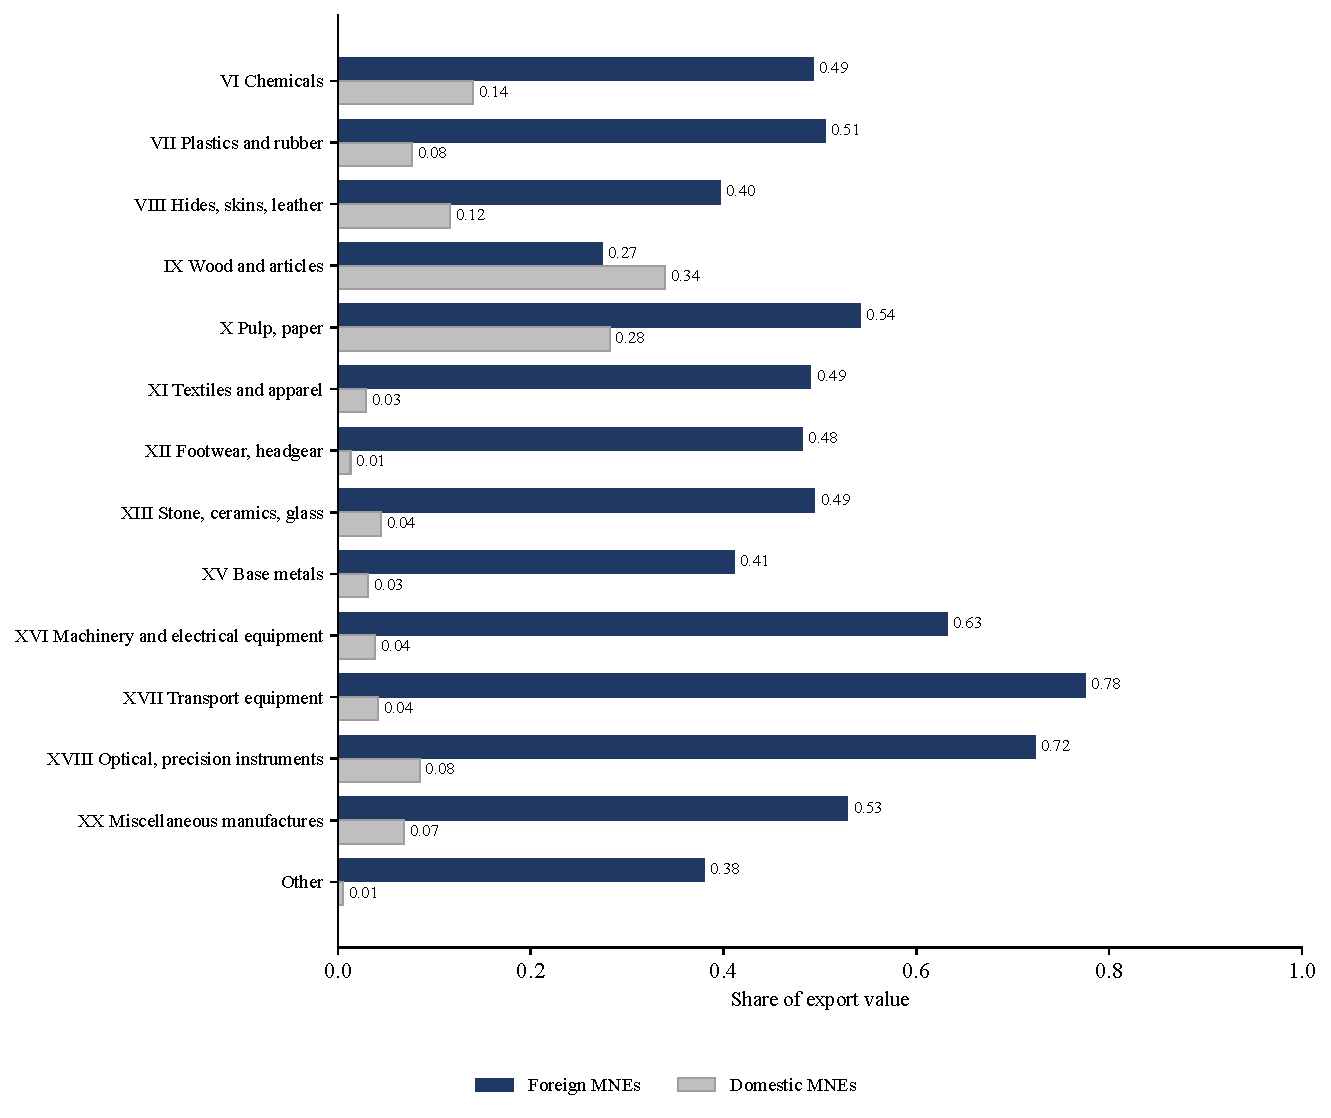
\includegraphics[width=0.9\textwidth,height=0.8\textheight,keepaspectratio]{figures/manufacturing/fig_wp2_hs_section.pdf}%
  \caption{Manufacturing: Multinational Share of Export Value, by HS Section}%
  \label{fig:sc_hs_section_f_manufacturing}%
  \par\vspace{2pt}%
  \parbox{0.92\textwidth}{\footnotesize %
  \textit{Notes:} Shares of manufacturing export value (HS 28--97 excluding 71), all available years pooled. HS sections.\\[3pt]%
  \textit{Source:} Authors' calculations based on customs data matched to Orbis and Dun \& Bradstreet.}%
  \end{figure}
% ---- Figure: Manufacturing: Foreign-Multinational Share of Export Value, by Exporting Country and HS Section
\begin{figure}[H]\centering%
  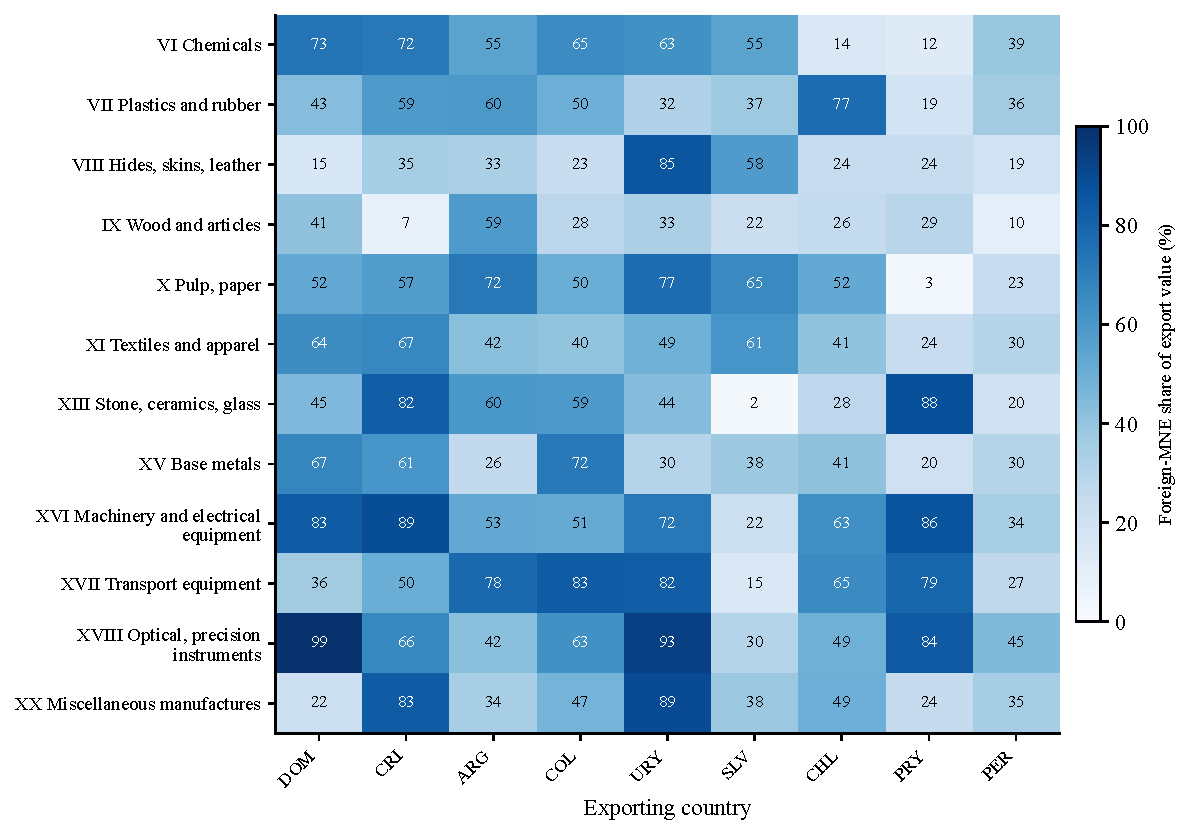
\includegraphics[width=0.95\textwidth,height=0.8\textheight,keepaspectratio]{figures/manufacturing/fig_wp2_origin_x_hs_section.pdf}%
  \caption{Manufacturing: Foreign-Multinational Share of Export Value, by Exporting Country and HS Section}%
  \label{fig:sc_hs_section_hm_manufacturing}%
  \par\vspace{2pt}%
  \parbox{0.92\textwidth}{\footnotesize %
  \textit{Notes:} Percent of each group's export value in each country shipped by foreign MNEs. HS sections.\\[3pt]%
  \textit{Source:} Authors' calculations based on customs data matched to Orbis and Dun \& Bradstreet.}%
  \end{figure}
% ---- Table: Manufacturing: Exports by Exporting Country and HS Section
\begin{table}[H]\centering\footnotesize%
  \caption{Manufacturing: Exports by Exporting Country and HS Section}%
  \label{tab:sc_hs_section_ht_manufacturing}%
  \adjustbox{max width=\textwidth, max totalheight=0.8\textheight}{\begin{tabular}{lrrrrrrrrrr}
\toprule
Sub-sector & ARG & CHL & COL & CRI & DOM & PER & PRY & SLV & URY & All \\
\midrule
\multicolumn{11}{l}{\textit{Panel A: composition of the origin's exports, \% (columns sum to 100)}} \\
VI Chemicals & 23.2 & 10.7 & 22.7 & 10.4 & 13.2 & 10.2 & 12.4 & 7.0 & 16.6 & 15.4 \\
VII Plastics and rubber & 6.8 & 2.2 & 17.9 & 10.0 & 7.0 & 7.0 & 10.3 & 7.6 & 22.3 & 7.8 \\
VIII Hides, skins, leather & 4.0 & 0.1 & 2.2 & 0.4 & 0.5 & 0.5 & 13.1 & 0.3 & 11.1 & 1.9 \\
IX Wood and articles & 0.8 & 7.0 & 0.5 & 1.2 & 0.2 & 1.8 & 7.5 & 0.2 & 11.7 & 3.0 \\
X Pulp, paper & 2.4 & 10.0 & 4.7 & 2.4 & 1.8 & 2.7 & 2.7 & 7.4 & 3.2 & 5.2 \\
XI Textiles and apparel & 2.6 & 0.3 & 9.6 & 2.6 & 21.0 & 20.0 & 17.0 & 58.2 & 12.7 & 9.5 \\
XII Footwear, headgear & 0.1 & 0.0 & 0.5 & 0.0 & 7.3 & 0.4 & 1.9 & 1.1 & 0.1 & 0.6 \\
XIII Stone, ceramics, glass & 0.7 & 0.2 & 3.9 & 2.0 & 0.6 & 2.6 & 1.6 & 1.0 & 0.4 & 1.3 \\
XV Base metals & 10.2 & 65.8 & 17.1 & 6.6 & 10.0 & 48.3 & 7.9 & 7.2 & 4.6 & 30.2 \\
XVI Machinery and electrical equipment & 8.2 & 2.3 & 9.9 & 24.8 & 16.6 & 4.3 & 18.5 & 7.5 & 4.0 & 8.0 \\
XVII Transport equipment & 39.6 & 1.0 & 6.4 & 0.6 & 0.4 & 0.9 & 3.2 & 0.2 & 8.2 & 11.4 \\
XVIII Optical, precision instruments & 0.8 & 0.1 & 1.0 & 35.9 & 20.3 & 0.2 & 1.6 & 0.1 & 1.5 & 4.1 \\
XX Miscellaneous manufactures & 0.5 & 0.2 & 3.4 & 3.1 & 1.1 & 0.9 & 2.2 & 2.1 & 3.5 & 1.3 \\
Other & 0.3 & 0.0 & 0.2 & 0.0 & 0.0 & 0.1 & 0.0 & 0.0 & 0.1 & 0.1 \\
All sub-sectors & 100.0 & 100.0 & 100.0 & 100.0 & 100.0 & 100.0 & 100.0 & 100.0 & 100.0 & 100.0 \\
\midrule
\multicolumn{11}{l}{\textit{Panel B: foreign-MNE share of export value, \%}} \\
VI Chemicals & 55.0 & 14.3 & 64.6 & 72.2 & 73.4 & 38.8 & 12.2 & 55.1 & 62.7 & 49.3 \\
VII Plastics and rubber & 59.7 & 76.7 & 49.5 & 59.0 & 43.3 & 36.2 & 18.5 & 37.2 & 32.0 & 50.5 \\
VIII Hides, skins, leather & 33.2 & 23.6 & 23.1 & 35.3 & 15.3 & 18.8 & 23.6 & 57.9 & 85.5 & 39.7 \\
IX Wood and articles & 58.9 & 25.7 & 27.8 & 7.3 & 41.1 & 9.7 & 29.1 & 21.9 & 33.4 & 27.4 \\
X Pulp, paper & 72.0 & 52.2 & 50.1 & 57.2 & 52.3 & 23.5 & 2.9 & 65.4 & 76.8 & 54.2 \\
XI Textiles and apparel & 42.5 & 40.6 & 40.1 & 66.6 & 64.3 & 30.0 & 24.1 & 60.8 & 48.6 & 49.1 \\
XII Footwear, headgear & 41.4 & 52.4 & 22.2 & 18.4 & 63.3 & 15.4 & 83.2 & 7.7 & 39.8 & 48.2 \\
XIII Stone, ceramics, glass & 59.8 & 27.6 & 59.4 & 82.3 & 45.0 & 19.7 & 87.8 & 2.2 & 43.6 & 49.5 \\
XV Base metals & 26.1 & 41.4 & 71.9 & 60.8 & 66.9 & 30.0 & 20.4 & 37.5 & 30.1 & 41.1 \\
XVI Machinery and electrical equipment & 52.5 & 63.2 & 51.3 & 88.7 & 83.1 & 34.0 & 86.0 & 21.7 & 72.2 & 63.2 \\
XVII Transport equipment & 78.1 & 65.2 & 82.9 & 50.3 & 36.2 & 27.0 & 79.4 & 14.6 & 82.0 & 77.6 \\
XVIII Optical, precision instruments & 42.1 & 49.2 & 62.9 & 65.7 & 99.2 & 44.9 & 83.8 & 30.3 & 93.5 & 72.3 \\
XX Miscellaneous manufactures & 34.4 & 49.2 & 47.3 & 83.0 & 21.6 & 34.8 & 24.5 & 38.0 & 89.3 & 52.9 \\
Other & 52.7 & 1.3 & 7.2 & 12.5 & 10.5 & 4.5 & 1.1 & 33.7 & 5.1 & 38.0 \\
All sub-sectors & 60.4 & 39.9 & 57.8 & 70.9 & 73.2 & 30.6 & 37.9 & 52.5 & 55.3 & 51.6 \\
\bottomrule
\end{tabular}
}%
  \par\vspace{3pt}%
  \begin{minipage}{0.95\textwidth}\footnotesize %
  \textit{Notes:} Panel A: composition of each country's exports in the sector (rows add to 100). Panel B: percent of each cell's export value shipped by foreign MNEs. HS sections.\\[3pt]%
  \textit{Source:} Authors' calculations based on customs data matched to Orbis and Dun \& Bradstreet.%
  \end{minipage}%
  \end{table}
% ---- Table: Manufacturing: Exports by HS Section and Parent Country
\begin{table}[H]\centering\footnotesize%
  \caption{Manufacturing: Exports by HS Section and Parent Country}%
  \label{tab:sc_hs_section_par_manufacturing}%
  \adjustbox{max width=\textwidth, max totalheight=0.8\textheight}{\begin{tabular}{lrrrrrrrrrrrr}
\toprule
HS section & USA & GBR & DEU & JPN & PAN & CAN & NLD & FRA & BRA & MEX & Other & Domestic \\
\midrule
VI Chemicals & 11.0 & 5.5 & 5.8 & 0.7 & 1.0 & 1.4 & 0.8 & 0.7 & 1.7 & 0.1 & 20.4 & 14.0 \\
VII Plastics and rubber & 15.7 & 1.8 & 0.7 & 2.7 & 1.8 & 2.3 & 1.8 & 1.3 & 1.9 & 8.0 & 12.6 & 7.7 \\
VIII Hides, skins, leather & 1.0 & 0.1 & 1.9 & 0.0 & 0.5 & 0.0 & 1.5 & 0.2 & 2.8 & 0.2 & 31.6 & 11.6 \\
IX Wood and articles & 2.4 & 0.5 & 0.1 & 2.7 & 0.1 & 1.2 & 0.0 & 0.3 & 0.1 & 0.1 & 19.8 & 33.9 \\
X Pulp, paper & 10.3 & 0.4 & 0.1 & 0.1 & 28.5 & 0.0 & 0.0 & 0.0 & 0.0 & 0.3 & 14.4 & 28.2 \\
XI Textiles and apparel & 25.8 & 1.2 & 0.5 & 0.7 & 0.9 & 1.6 & 0.0 & 1.4 & 0.4 & 0.1 & 16.6 & 2.9 \\
XII Footwear, headgear & 27.8 & 0.1 & 0.9 & 3.5 & 0.0 & 0.0 & 0.0 & 0.6 & 5.3 & 0.0 & 9.9 & 1.3 \\
XIII Stone, ceramics, glass & 13.0 & 2.1 & 1.9 & 0.2 & 8.0 & 0.0 & 2.6 & 2.4 & 0.5 & 2.3 & 16.6 & 4.5 \\
XV Base metals & 2.5 & 17.1 & 0.1 & 0.2 & 0.5 & 4.5 & 0.8 & 0.5 & 2.9 & 0.4 & 11.8 & 3.1 \\
XVI Machinery and electrical equipment & 24.5 & 1.7 & 2.3 & 4.5 & 0.3 & 1.2 & 1.6 & 2.9 & 0.8 & 2.4 & 21.1 & 3.9 \\
XVII Transport equipment & 7.6 & 0.1 & 23.2 & 21.8 & 0.0 & 0.2 & 9.5 & 8.6 & 0.9 & 0.0 & 5.7 & 4.2 \\
XVIII Optical, precision instruments & 43.8 & 5.1 & 7.7 & 2.8 & 0.1 & 0.2 & 0.3 & 0.7 & 0.1 & 0.0 & 11.6 & 8.5 \\
XX Miscellaneous manufactures & 21.9 & 1.4 & 4.3 & 1.5 & 0.5 & 0.0 & 0.7 & 2.3 & 0.1 & 0.9 & 19.2 & 6.9 \\
Other & 0.6 & 0.1 & 0.0 & 0.0 & 0.0 & 0.0 & 0.1 & 0.0 & 0.0 & 0.0 & 37.3 & 0.5 \\
\bottomrule
\end{tabular}
}%
  \par\vspace{3pt}%
  \begin{minipage}{0.95\textwidth}\footnotesize %
  \textit{Notes:} Percent of each group's export value, by country of the ultimate parent of foreign MNEs; domestic MNEs shown for comparison. HS sections.\\[3pt]%
  \textit{Source:} Authors' calculations based on customs data matched to Orbis and Dun \& Bradstreet.%
  \end{minipage}%
  \end{table}

\subsection{By End Use}
% ---- Table: Manufacturing: Exports and Multinational Shares, by End Use
\begin{table}[H]\centering\footnotesize%
  \caption{Manufacturing: Exports and Multinational Shares, by End Use}%
  \label{tab:sc_bec_enduse_manufacturing}%
  \adjustbox{max width=\textwidth, max totalheight=0.8\textheight}{\begin{tabular}{@{}l r r r r l@{}}
\toprule
BEC end use & Total exports (US\$bn/yr) & MNE exports (US\$bn/yr) & Foreign (\%) & Domestic (\%) & Leading parents (share of foreign) \\
\midrule
Intermediate & 47.2 & 26.6 & 46.9 & 9.1 & GBR 0.20, USA 0.20, PAN 0.07 \\
Consumption & 15.2 & 10.0 & 60.6 & 4.9 & USA 0.43, NLD 0.09, DEU 0.08 \\
Capital & 9.3 & 6.7 & 64.8 & 5.6 & DEU 0.31, JPN 0.28, USA 0.18 \\
\midrule
All & 71.7 & 43.3 & 51.7 & 7.8 & \\
\bottomrule
\end{tabular}
}%
  \par\vspace{3pt}%
  \begin{minipage}{0.95\textwidth}\footnotesize %
  \textit{Notes:} End use from BEC Rev.\,4. Foreign and domestic: percent of the group's export value. Leading parents: the three largest parent countries and their share of the row's foreign-MNE exports. Values are annual averages in US\$ billion.\\[3pt]%
  \textit{Source:} Authors' calculations based on customs data matched to Orbis and Dun \& Bradstreet.%
  \end{minipage}%
  \end{table}
% ---- Figure: Manufacturing: Multinational Share of Export Value, by End Use
\begin{figure}[H]\centering%
  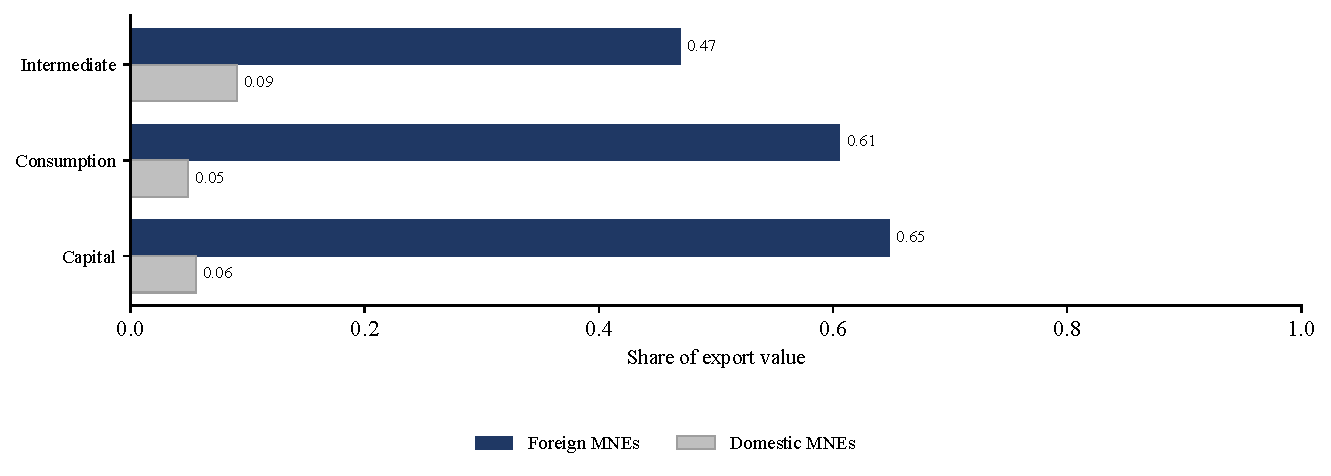
\includegraphics[width=0.9\textwidth,height=0.8\textheight,keepaspectratio]{figures/manufacturing/fig_wp2_bec_enduse.pdf}%
  \caption{Manufacturing: Multinational Share of Export Value, by End Use}%
  \label{fig:sc_bec_enduse_f_manufacturing}%
  \par\vspace{2pt}%
  \parbox{0.92\textwidth}{\footnotesize %
  \textit{Notes:} Shares of manufacturing export value (HS 28--97 excluding 71), all available years pooled. End use from BEC Rev.\,4.\\[3pt]%
  \textit{Source:} Authors' calculations based on customs data matched to Orbis and Dun \& Bradstreet.}%
  \end{figure}
% ---- Figure: Manufacturing: Foreign-Multinational Share of Export Value, by Exporting Country and End Use
\begin{figure}[H]\centering%
  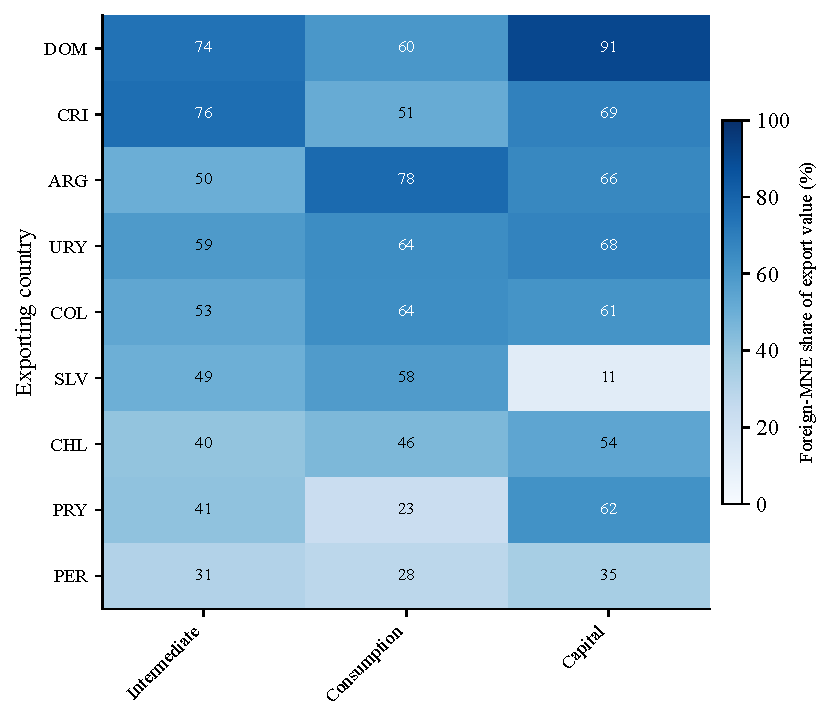
\includegraphics[width=0.95\textwidth,height=0.8\textheight,keepaspectratio]{figures/manufacturing/fig_wp2_origin_x_bec_enduse.pdf}%
  \caption{Manufacturing: Foreign-Multinational Share of Export Value, by Exporting Country and End Use}%
  \label{fig:sc_bec_enduse_hm_manufacturing}%
  \par\vspace{2pt}%
  \parbox{0.92\textwidth}{\footnotesize %
  \textit{Notes:} Percent of each group's export value in each country shipped by foreign MNEs. End use from BEC Rev.\,4.\\[3pt]%
  \textit{Source:} Authors' calculations based on customs data matched to Orbis and Dun \& Bradstreet.}%
  \end{figure}
% ---- Table: Manufacturing: Exports by Exporting Country and End Use
\begin{table}[H]\centering\footnotesize%
  \caption{Manufacturing: Exports by Exporting Country and End Use}%
  \label{tab:sc_bec_enduse_ht_manufacturing}%
  \adjustbox{max width=\textwidth, max totalheight=0.8\textheight}{\begin{tabular}{lrrrr}
\toprule
Origin & Intermediate & Consumption & Capital & All \\
\midrule
\multicolumn{5}{l}{\textit{Panel A: composition of the origin's exports, \% (rows sum to 100)}} \\
ARG & 51.1 & 22.3 & 26.7 & 100.0 \\
CHL & 96.6 & 1.5 & 1.9 & 100.0 \\
COL & 60.5 & 32.5 & 7.0 & 100.0 \\
CRI & 66.5 & 19.0 & 14.6 & 100.0 \\
DOM & 42.9 & 34.3 & 22.8 & 100.0 \\
PER & 76.1 & 20.6 & 3.3 & 100.0 \\
PRY & 70.4 & 23.6 & 5.9 & 100.0 \\
SLV & 29.3 & 64.0 & 6.7 & 100.0 \\
URY & 78.3 & 15.4 & 6.4 & 100.0 \\
All origins & 68.3 & 20.3 & 11.4 & 100.0 \\
\midrule
\multicolumn{5}{l}{\textit{Panel B: foreign-MNE share of export value, \%}} \\
ARG & 49.9 & 77.7 & 66.3 & 60.4 \\
CHL & 39.9 & 45.7 & 53.6 & 40.3 \\
COL & 53.5 & 63.9 & 61.4 & 57.4 \\
CRI & 76.0 & 51.0 & 68.6 & 70.2 \\
DOM & 74.3 & 60.1 & 90.6 & 73.2 \\
PER & 31.2 & 27.8 & 34.5 & 30.6 \\
PRY & 40.8 & 23.0 & 62.2 & 37.9 \\
SLV & 49.4 & 58.2 & 11.0 & 52.4 \\
URY & 58.7 & 64.1 & 67.9 & 60.2 \\
All origins & 46.9 & 60.6 & 64.8 & 51.7 \\
\bottomrule
\end{tabular}
}%
  \par\vspace{3pt}%
  \begin{minipage}{0.95\textwidth}\footnotesize %
  \textit{Notes:} Panel A: composition of each country's exports in the sector (rows add to 100). Panel B: percent of each cell's export value shipped by foreign MNEs. End use from BEC Rev.\,4.\\[3pt]%
  \textit{Source:} Authors' calculations based on customs data matched to Orbis and Dun \& Bradstreet.%
  \end{minipage}%
  \end{table}
% ---- Table: Manufacturing: Exports by End Use and Parent Country
\begin{table}[H]\centering\footnotesize%
  \caption{Manufacturing: Exports by End Use and Parent Country}%
  \label{tab:sc_bec_enduse_par_manufacturing}%
  \adjustbox{max width=\textwidth, max totalheight=0.8\textheight}{\begin{tabular}{lrrrrrrrrrrrr}
\toprule
BEC end use & USA & GBR & DEU & JPN & PAN & CAN & NLD & FRA & BRA & MEX & Other & Domestic \\
\midrule
Intermediate & 8.5 & 8.6 & 1.9 & 1.2 & 2.9 & 2.8 & 1.1 & 1.2 & 2.0 & 1.2 & 15.5 & 9.1 \\
Consumption & 23.9 & 3.3 & 4.6 & 4.1 & 0.8 & 0.5 & 4.8 & 4.0 & 0.8 & 1.0 & 12.8 & 4.9 \\
Capital & 10.7 & 1.9 & 19.1 & 16.9 & 0.2 & 0.5 & 0.7 & 1.5 & 0.9 & 0.3 & 12.0 & 5.6 \\
\bottomrule
\end{tabular}
}%
  \par\vspace{3pt}%
  \begin{minipage}{0.95\textwidth}\footnotesize %
  \textit{Notes:} Percent of each group's export value, by country of the ultimate parent of foreign MNEs; domestic MNEs shown for comparison. End use from BEC Rev.\,4.\\[3pt]%
  \textit{Source:} Authors' calculations based on customs data matched to Orbis and Dun \& Bradstreet.%
  \end{minipage}%
  \end{table}

\subsection{By BEC Category}
% ---- Table: Manufacturing: Exports and Multinational Shares, by BEC Category
\begin{table}[H]\centering\footnotesize%
  \caption{Manufacturing: Exports and Multinational Shares, by BEC Category}%
  \label{tab:sc_bec4_manufacturing}%
  \adjustbox{max width=\textwidth, max totalheight=0.8\textheight}{\begin{tabular}{@{}l r r r r l@{}}
\toprule
BEC Rev.\,4 category & Total exports (US\$bn/yr) & MNE exports (US\$bn/yr) & Foreign (\%) & Domestic (\%) & Leading parents (share of foreign) \\
\midrule
22 Industrial supplies, processed & 39.4 & 21.5 & 44.6 & 10.0 & GBR 0.24, USA 0.16, PAN 0.08 \\
63 Consumer goods, non-durable & 7.4 & 5.0 & 62.6 & 5.3 & USA 0.54, DEU 0.13, GBR 0.08 \\
521 Transport equipment, industrial & 4.9 & 4.0 & 74.1 & 7.1 & DEU 0.42, JPN 0.42, CHL 0.07 \\
41 Capital goods & 4.4 & 2.6 & 55.0 & 3.9 & USA 0.45, DEU 0.14, GBR 0.08 \\
62 Consumer goods, semi-durable & 3.8 & 1.7 & 42.3 & 2.3 & USA 0.49, GBR 0.10, CHE 0.05 \\
51 Passenger cars & 3.1 & 2.7 & 88.5 & 0.0 & NLD 0.29, USA 0.23, FRA 0.21 \\
53 Parts of transport equipment & 2.9 & 2.2 & 74.3 & 2.1 & DEU 0.31, USA 0.22, JPN 0.17 \\
42 Parts of capital goods & 2.9 & 2.2 & 72.0 & 3.3 & USA 0.56, IRL 0.19, GBR 0.05 \\
21 Industrial supplies, primary & 1.8 & 0.6 & 26.1 & 7.3 & JPN 0.20, BGR 0.11, GBR 0.09 \\
61 Consumer goods, durable & 0.9 & 0.6 & 35.1 & 27.8 & MEX 0.43, USA 0.10, JPN 0.09 \\
Other & 0.2 & 0.1 & 39.8 & 3.1 & JPN 0.32, ESP 0.23, DEU 0.09 \\
\midrule
All & 71.7 & 43.3 & 51.7 & 7.8 & \\
\bottomrule
\end{tabular}
}%
  \par\vspace{3pt}%
  \begin{minipage}{0.95\textwidth}\footnotesize %
  \textit{Notes:} Categories of BEC Rev.\,4. Foreign and domestic: percent of the group's export value. Leading parents: the three largest parent countries and their share of the row's foreign-MNE exports. Values are annual averages in US\$ billion.\\[3pt]%
  \textit{Source:} Authors' calculations based on customs data matched to Orbis and Dun \& Bradstreet.%
  \end{minipage}%
  \end{table}
% ---- Figure: Manufacturing: Multinational Share of Export Value, by BEC Category
\begin{figure}[H]\centering%
  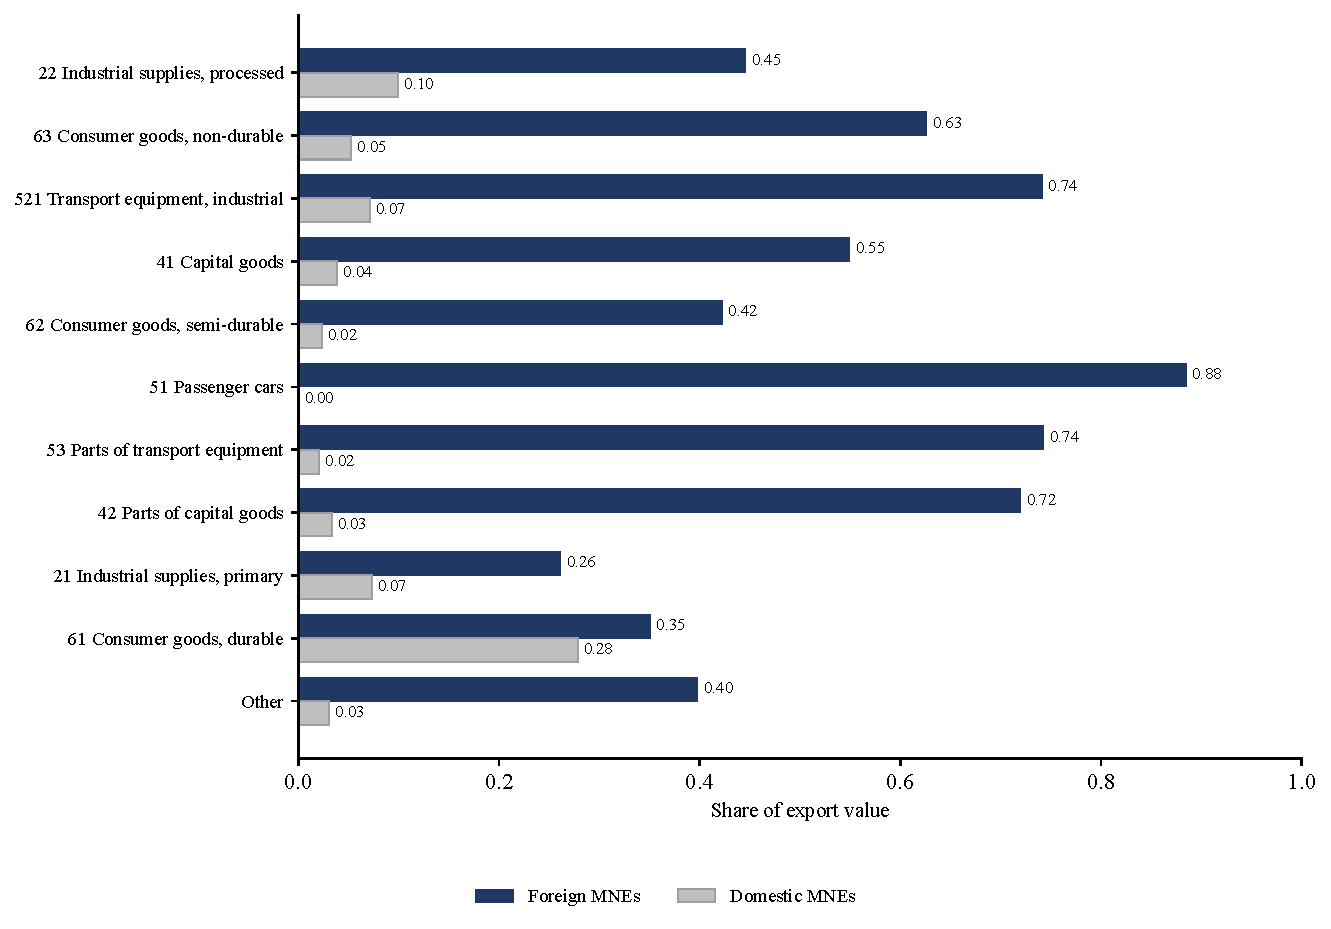
\includegraphics[width=0.9\textwidth,height=0.8\textheight,keepaspectratio]{figures/manufacturing/fig_wp2_bec4.pdf}%
  \caption{Manufacturing: Multinational Share of Export Value, by BEC Category}%
  \label{fig:sc_bec4_f_manufacturing}%
  \par\vspace{2pt}%
  \parbox{0.92\textwidth}{\footnotesize %
  \textit{Notes:} Shares of manufacturing export value (HS 28--97 excluding 71), all available years pooled. Categories of BEC Rev.\,4.\\[3pt]%
  \textit{Source:} Authors' calculations based on customs data matched to Orbis and Dun \& Bradstreet.}%
  \end{figure}
% ---- Figure: Manufacturing: Foreign-Multinational Share of Export Value, by Exporting Country and BEC Category
\begin{figure}[H]\centering%
  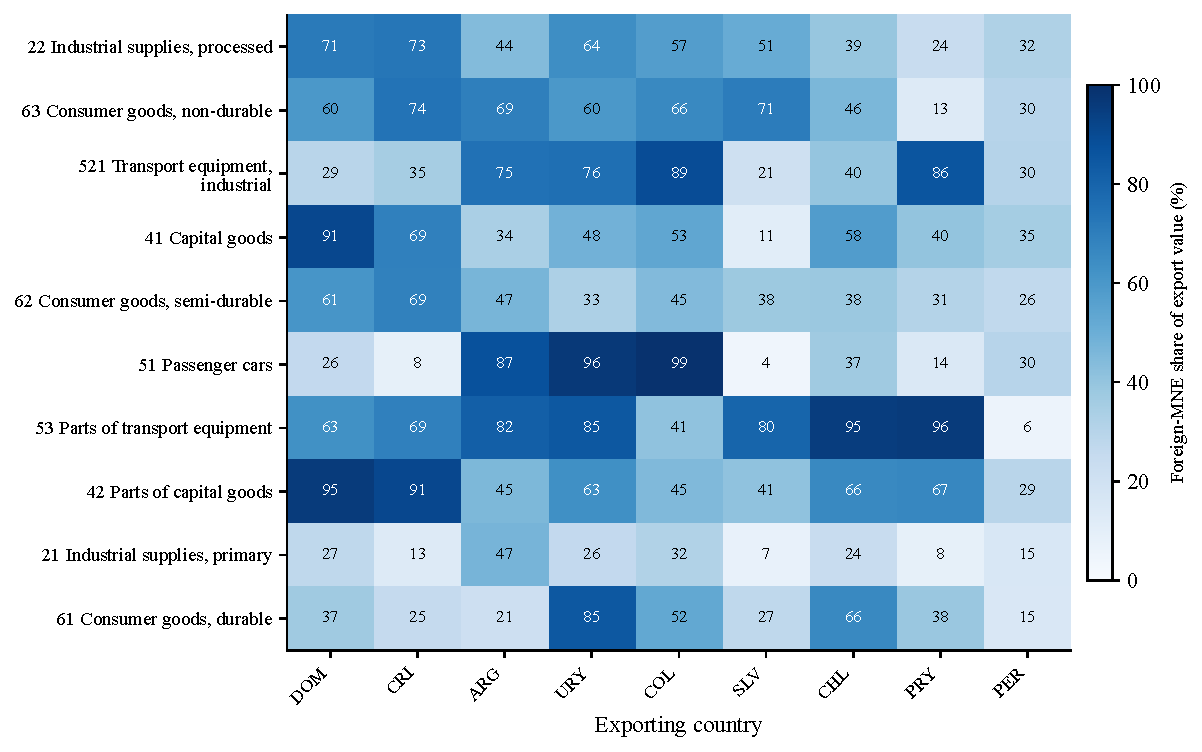
\includegraphics[width=0.95\textwidth,height=0.8\textheight,keepaspectratio]{figures/manufacturing/fig_wp2_origin_x_bec4.pdf}%
  \caption{Manufacturing: Foreign-Multinational Share of Export Value, by Exporting Country and BEC Category}%
  \label{fig:sc_bec4_hm_manufacturing}%
  \par\vspace{2pt}%
  \parbox{0.92\textwidth}{\footnotesize %
  \textit{Notes:} Percent of each group's export value in each country shipped by foreign MNEs. Categories of BEC Rev.\,4.\\[3pt]%
  \textit{Source:} Authors' calculations based on customs data matched to Orbis and Dun \& Bradstreet.}%
  \end{figure}
% ---- Table: Manufacturing: Exports by Exporting Country and BEC Category
\begin{table}[H]\centering\footnotesize%
  \caption{Manufacturing: Exports by Exporting Country and BEC Category}%
  \label{tab:sc_bec4_ht_manufacturing}%
  \adjustbox{max width=\textwidth, max totalheight=0.8\textheight}{\begin{tabular}{lrrrrrrrrrr}
\toprule
Sub-sector & ARG & CHL & COL & CRI & DOM & PER & PRY & SLV & URY & All \\
\midrule
\multicolumn{11}{l}{\textit{Panel A: composition of the origin's exports, \% (columns sum to 100)}} \\
22 Industrial supplies, processed & 39.2 & 91.5 & 48.9 & 41.1 & 27.6 & 71.5 & 42.0 & 26.1 & 60.3 & 58.2 \\
63 Consumer goods, non-durable & 8.4 & 1.0 & 19.5 & 8.1 & 13.4 & 10.4 & 10.3 & 40.1 & 9.2 & 10.2 \\
521 Transport equipment, industrial & 21.0 & 0.4 & 1.6 & 0.1 & 0.1 & 0.6 & 2.9 & 0.1 & 4.6 & 5.8 \\
41 Capital goods & 5.6 & 1.5 & 5.4 & 14.4 & 22.7 & 2.7 & 3.1 & 6.7 & 1.8 & 5.5 \\
62 Consumer goods, semi-durable & 0.9 & 0.2 & 7.1 & 2.3 & 20.5 & 9.9 & 12.2 & 23.1 & 2.2 & 5.1 \\
51 Passenger cars & 12.6 & 0.1 & 3.5 & 0.0 & 0.0 & 0.0 & 0.1 & 0.0 & 2.6 & 3.7 \\
53 Parts of transport equipment & 7.7 & 1.5 & 3.8 & 3.3 & 0.7 & 1.4 & 15.5 & 1.0 & 4.3 & 3.7 \\
42 Parts of capital goods & 2.8 & 0.9 & 3.0 & 19.8 & 11.5 & 1.7 & 2.4 & 0.6 & 0.9 & 3.7 \\
21 Industrial supplies, primary & 1.0 & 2.7 & 4.5 & 2.2 & 3.2 & 1.4 & 7.1 & 1.6 & 12.7 & 2.6 \\
61 Consumer goods, durable & 0.3 & 0.1 & 2.3 & 8.6 & 0.3 & 0.3 & 1.1 & 0.7 & 1.3 & 1.2 \\
Other & 0.3 & 0.0 & 0.4 & 0.1 & 0.1 & 0.1 & 3.5 & 0.1 & 0.1 & 0.2 \\
All sub-sectors & 100.0 & 100.0 & 100.0 & 100.0 & 100.0 & 100.0 & 100.0 & 100.0 & 100.0 & 100.0 \\
\midrule
\multicolumn{11}{l}{\textit{Panel B: foreign-MNE share of export value, \%}} \\
22 Industrial supplies, processed & 44.1 & 39.2 & 57.2 & 72.9 & 71.4 & 32.1 & 24.1 & 51.0 & 63.8 & 44.6 \\
63 Consumer goods, non-durable & 69.2 & 45.8 & 65.9 & 73.8 & 59.7 & 29.7 & 12.5 & 70.6 & 59.7 & 62.6 \\
521 Transport equipment, industrial & 74.9 & 39.6 & 88.8 & 35.0 & 29.2 & 30.4 & 85.8 & 20.6 & 75.6 & 74.1 \\
41 Capital goods & 34.0 & 57.8 & 53.5 & 69.0 & 90.9 & 35.4 & 40.0 & 10.9 & 48.1 & 55.0 \\
62 Consumer goods, semi-durable & 46.5 & 38.1 & 44.5 & 68.5 & 60.8 & 26.2 & 30.5 & 37.7 & 32.7 & 42.3 \\
51 Passenger cars & 87.2 & 37.0 & 98.9 & 8.3 & 26.0 & 29.7 & 14.4 & 4.1 & 96.2 & 88.5 \\
53 Parts of transport equipment & 81.9 & 94.9 & 40.7 & 69.1 & 62.7 & 5.7 & 95.6 & 79.6 & 84.5 & 74.3 \\
42 Parts of capital goods & 45.4 & 66.0 & 44.6 & 90.8 & 95.4 & 28.9 & 66.5 & 41.0 & 63.3 & 72.0 \\
21 Industrial supplies, primary & 47.1 & 23.9 & 31.6 & 13.1 & 27.1 & 15.4 & 8.2 & 7.5 & 25.9 & 26.1 \\
61 Consumer goods, durable & 21.3 & 65.8 & 52.4 & 25.2 & 37.1 & 15.2 & 38.4 & 27.1 & 84.5 & 35.1 \\
Other & 37.9 & 17.7 & 42.9 & 47.7 & 15.0 & 59.2 & 46.2 & 8.8 & 58.4 & 39.8 \\
All sub-sectors & 60.4 & 40.3 & 57.4 & 70.2 & 73.2 & 30.6 & 37.9 & 52.4 & 60.2 & 51.7 \\
\bottomrule
\end{tabular}
}%
  \par\vspace{3pt}%
  \begin{minipage}{0.95\textwidth}\footnotesize %
  \textit{Notes:} Panel A: composition of each country's exports in the sector (rows add to 100). Panel B: percent of each cell's export value shipped by foreign MNEs. Categories of BEC Rev.\,4.\\[3pt]%
  \textit{Source:} Authors' calculations based on customs data matched to Orbis and Dun \& Bradstreet.%
  \end{minipage}%
  \end{table}
% ---- Table: Manufacturing: Exports by BEC Category and Parent Country
\begin{table}[H]\centering\footnotesize%
  \caption{Manufacturing: Exports by BEC Category and Parent Country}%
  \label{tab:sc_bec4_par_manufacturing}%
  \adjustbox{max width=\textwidth, max totalheight=0.8\textheight}{\begin{tabular}{lrrrrrrrrrrrr}
\toprule
BEC Rev.\,4 category & USA & GBR & DEU & JPN & PAN & CAN & NLD & FRA & BRA & MEX & Other & Domestic \\
\midrule
22 Industrial supplies, processed & 6.5 & 9.8 & 0.6 & 0.4 & 3.4 & 3.2 & 1.0 & 0.9 & 2.2 & 1.4 & 15.2 & 10.0 \\
63 Consumer goods, non-durable & 31.4 & 4.7 & 7.3 & 1.0 & 1.1 & 0.9 & 0.1 & 0.5 & 1.2 & 0.3 & 14.3 & 5.3 \\
521 Transport equipment, industrial & 0.3 & 0.1 & 31.0 & 30.6 & 0.0 & 0.1 & 0.5 & 1.9 & 1.4 & 0.0 & 8.2 & 7.1 \\
41 Capital goods & 21.8 & 3.9 & 6.6 & 2.4 & 0.4 & 0.9 & 0.9 & 1.0 & 0.5 & 0.6 & 16.0 & 3.9 \\
62 Consumer goods, semi-durable & 16.4 & 3.4 & 1.3 & 0.5 & 1.0 & 0.0 & 0.2 & 0.6 & 0.8 & 0.2 & 17.8 & 2.3 \\
51 Passenger cars & 20.5 & 0.0 & 3.4 & 17.9 & 0.0 & 0.0 & 25.7 & 19.0 & 0.0 & 0.0 & 2.0 & 0.0 \\
53 Parts of transport equipment & 15.9 & 0.2 & 22.8 & 12.3 & 0.1 & 1.1 & 4.6 & 6.4 & 1.3 & 0.1 & 9.7 & 2.1 \\
42 Parts of capital goods & 38.4 & 3.4 & 1.6 & 1.0 & 0.2 & 0.9 & 1.0 & 2.1 & 0.3 & 0.2 & 22.9 & 3.3 \\
21 Industrial supplies, primary & 0.9 & 1.5 & 0.6 & 3.2 & 0.4 & 0.0 & 0.0 & 0.5 & 0.6 & 0.1 & 18.3 & 7.3 \\
61 Consumer goods, durable & 3.2 & 0.2 & 0.1 & 2.8 & 1.0 & 0.0 & 0.1 & 1.8 & 0.1 & 13.7 & 12.0 & 27.8 \\
Other & 1.3 & 0.2 & 2.5 & 8.8 & 0.0 & 0.4 & 0.0 & 0.2 & 0.9 & 0.0 & 25.5 & 3.1 \\
\bottomrule
\end{tabular}
}%
  \par\vspace{3pt}%
  \begin{minipage}{0.95\textwidth}\footnotesize %
  \textit{Notes:} Percent of each group's export value, by country of the ultimate parent of foreign MNEs; domestic MNEs shown for comparison. Categories of BEC Rev.\,4.\\[3pt]%
  \textit{Source:} Authors' calculations based on customs data matched to Orbis and Dun \& Bradstreet.%
  \end{minipage}%
  \end{table}

\subsection{By SITC Division}
% ---- Table: Manufacturing: Exports and Multinational Shares, by SITC Division
\begin{table}[H]\centering\footnotesize%
  \caption{Manufacturing: Exports and Multinational Shares, by SITC Division}%
  \label{tab:sc_sitc2_manufacturing}%
  \adjustbox{max width=\textwidth, max totalheight=0.8\textheight}{\begin{tabular}{@{}l r r r r l@{}}
\toprule
SITC Rev.\,3 division & Total exports (US\$bn/yr) & MNE exports (US\$bn/yr) & Foreign (\%) & Domestic (\%) & Leading parents (share of foreign) \\
\midrule
68 Non-ferrous metals & 14.5 & 5.7 & 38.6 & 2.2 & GBR 0.59, CAN 0.16, BRA 0.09 \\
78 Road vehicles & 8.5 & 7.2 & 84.0 & 0.7 & DEU 0.32, JPN 0.30, NLD 0.13 \\
84 Apparel & 4.5 & 2.3 & 51.5 & 1.0 & USA 0.73, CHE 0.04, CAN 0.03 \\
77 Electrical machinery & 3.2 & 2.5 & 74.7 & 0.9 & USA 0.46, IRL 0.15, JPN 0.11 \\
89 Misc. manufactures & 2.9 & 1.8 & 41.0 & 18.9 & USA 0.29, GBR 0.15, CAN 0.12 \\
67 Iron \& steel & 2.8 & 1.7 & 55.9 & 7.9 & ZAF 0.47, SGP 0.10, NLD 0.10 \\
59 Chemical materials n.e.s. & 3.0 & 1.9 & 57.6 & 8.5 & USA 0.29, DEU 0.23, LIE 0.14 \\
87 Instruments & 2.7 & 2.3 & 83.2 & 0.8 & USA 0.69, DEU 0.12, GBR 0.07 \\
52 Inorganic chemicals & 1.9 & 1.1 & 24.7 & 30.7 & USA 0.36, AUS 0.12, BRA 0.08 \\
54 Pharmaceuticals & 2.2 & 1.4 & 56.8 & 6.7 & USA 0.21, DEU 0.13, CHE 0.12 \\
57 Plastics, primary & 1.9 & 1.2 & 56.4 & 5.2 & MEX 0.38, USA 0.30, NLD 0.07 \\
55 Essential oils, cosmetics & 2.0 & 1.4 & 62.6 & 11.8 & GBR 0.32, USA 0.25, BRA 0.09 \\
25 Pulp \& paper & 1.5 & 1.5 & 63.5 & 35.1 & PAN 0.89, CHL 0.10, IRL 0.00 \\
65 Textile yarn \& fabrics & 1.7 & 0.9 & 41.8 & 7.8 & USA 0.51, CAN 0.09, GBR 0.05 \\
64 Paper & 1.6 & 1.1 & 48.7 & 22.6 & USA 0.46, IRL 0.14, ZAF 0.08 \\
69 Metal manufactures & 1.3 & 0.8 & 57.5 & 4.7 & USA 0.26, CYM 0.22, JPN 0.06 \\
61 Leather & 1.4 & 0.8 & 42.0 & 12.8 & BGR 0.19, URY 0.18, SGP 0.17 \\
58 Plastics, non-primary & 1.2 & 0.7 & 49.8 & 11.0 & USA 0.24, GBR 0.13, PAN 0.08 \\
24 Cork \& wood & 1.0 & 0.4 & 20.9 & 21.1 & JPN 0.34, CHL 0.16, USA 0.10 \\
74 General industrial machinery & 1.2 & 0.7 & 47.2 & 10.4 & USA 0.24, GBR 0.08, ITA 0.07 \\
79 Other transport equipment & 1.2 & 0.7 & 31.8 & 29.2 & CHL 0.66, BHS 0.11, ESP 0.03 \\
28 Metalliferous ores & 0.9 & 0.2 & 21.9 & 3.2 & BGR 0.29, TUR 0.12, BRA 0.11 \\
62 Rubber manufactures & 0.9 & 0.5 & 57.1 & 1.1 & USA 0.55, JPN 0.23, CHN 0.11 \\
66 Non-metallic mineral mfg & 0.9 & 0.5 & 53.7 & 4.5 & USA 0.31, PAN 0.19, CYM 0.11 \\
63 Cork \& wood manufactures & 0.7 & 0.6 & 42.2 & 41.3 & BHS 0.31, VGB 0.16, USA 0.11 \\
51 Organic chemicals & 0.8 & 0.5 & 53.6 & 8.0 & CAN 0.29, USA 0.23, GBR 0.12 \\
72 Specialised machinery & 0.7 & 0.3 & 41.0 & 7.0 & USA 0.19, CAN 0.10, GBR 0.08 \\
26 Textile fibres & 0.8 & 0.4 & 49.9 & 4.2 & FRA 0.28, GBR 0.16, CYM 0.14 \\
56 Fertilisers & 0.6 & 0.3 & 21.6 & 34.5 & VEN 0.39, PAN 0.17, CHE 0.10 \\
53 Dyeing materials & 0.6 & 0.3 & 49.2 & 6.9 & USA 0.31, LUX 0.13, NLD 0.10 \\
71 Power machinery & 0.6 & 0.4 & 66.1 & 2.7 & USA 0.31, DEU 0.14, ITA 0.12 \\
85 Footwear & 0.5 & 0.3 & 50.1 & 1.2 & USA 0.67, BRA 0.13, JPN 0.08 \\
82 Furniture & 0.4 & 0.2 & 40.3 & 2.0 & CHL 0.21, DEU 0.19, FRA 0.18 \\
Other & 1.2 & 0.5 & 40.4 & 4.0 & USA 0.48, GBR 0.09, MEX 0.04 \\
\midrule
All & 71.7 & 43.3 & 51.7 & 7.8 & \\
\bottomrule
\end{tabular}
}%
  \par\vspace{3pt}%
  \begin{minipage}{0.95\textwidth}\footnotesize %
  \textit{Notes:} SITC Rev.\,3 divisions; HS6 products without an SITC correspondence are excluded. Foreign and domestic: percent of the group's export value. Leading parents: the three largest parent countries and their share of the row's foreign-MNE exports. Values are annual averages in US\$ billion.\\[3pt]%
  \textit{Source:} Authors' calculations based on customs data matched to Orbis and Dun \& Bradstreet.%
  \end{minipage}%
  \end{table}
% ---- Figure: Manufacturing: Multinational Share of Export Value, by SITC Division
\begin{figure}[H]\centering%
  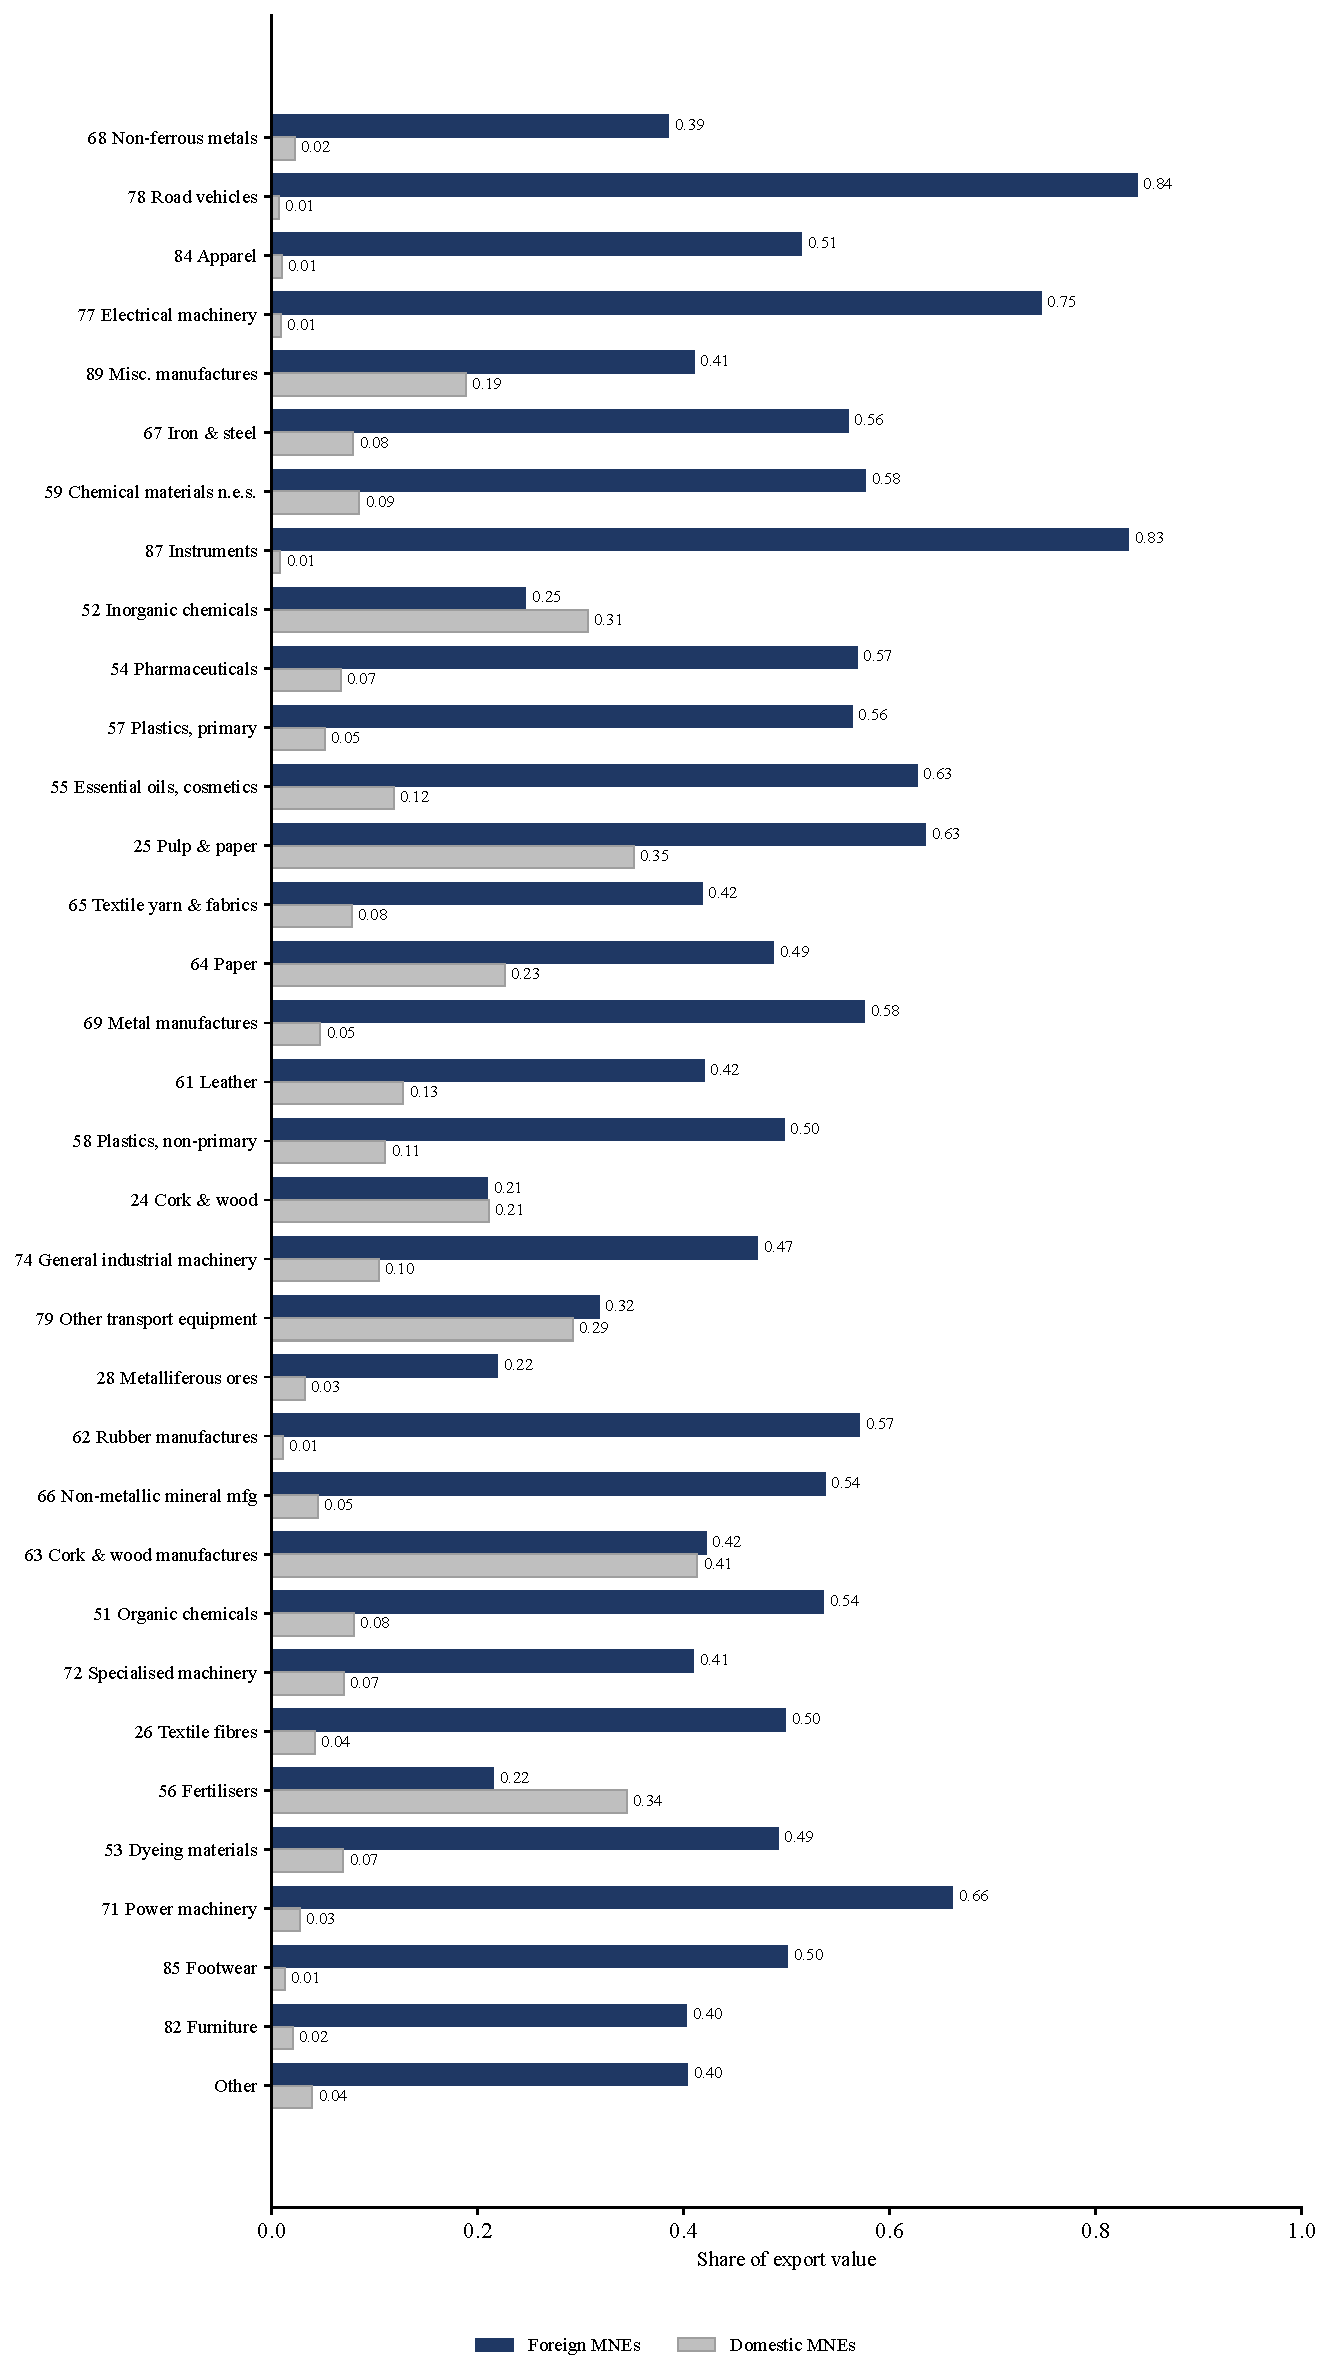
\includegraphics[width=0.9\textwidth,height=0.8\textheight,keepaspectratio]{figures/manufacturing/fig_wp2_sitc2.pdf}%
  \caption{Manufacturing: Multinational Share of Export Value, by SITC Division}%
  \label{fig:sc_sitc2_f_manufacturing}%
  \par\vspace{2pt}%
  \parbox{0.92\textwidth}{\footnotesize %
  \textit{Notes:} Shares of manufacturing export value (HS 28--97 excluding 71), all available years pooled. SITC Rev.\,3 divisions; HS6 products without an SITC correspondence are excluded.\\[3pt]%
  \textit{Source:} Authors' calculations based on customs data matched to Orbis and Dun \& Bradstreet.}%
  \end{figure}
% ---- Figure: Manufacturing: Foreign-Multinational Share of Export Value, by Exporting Country and SITC Division
\begin{figure}[H]\centering%
  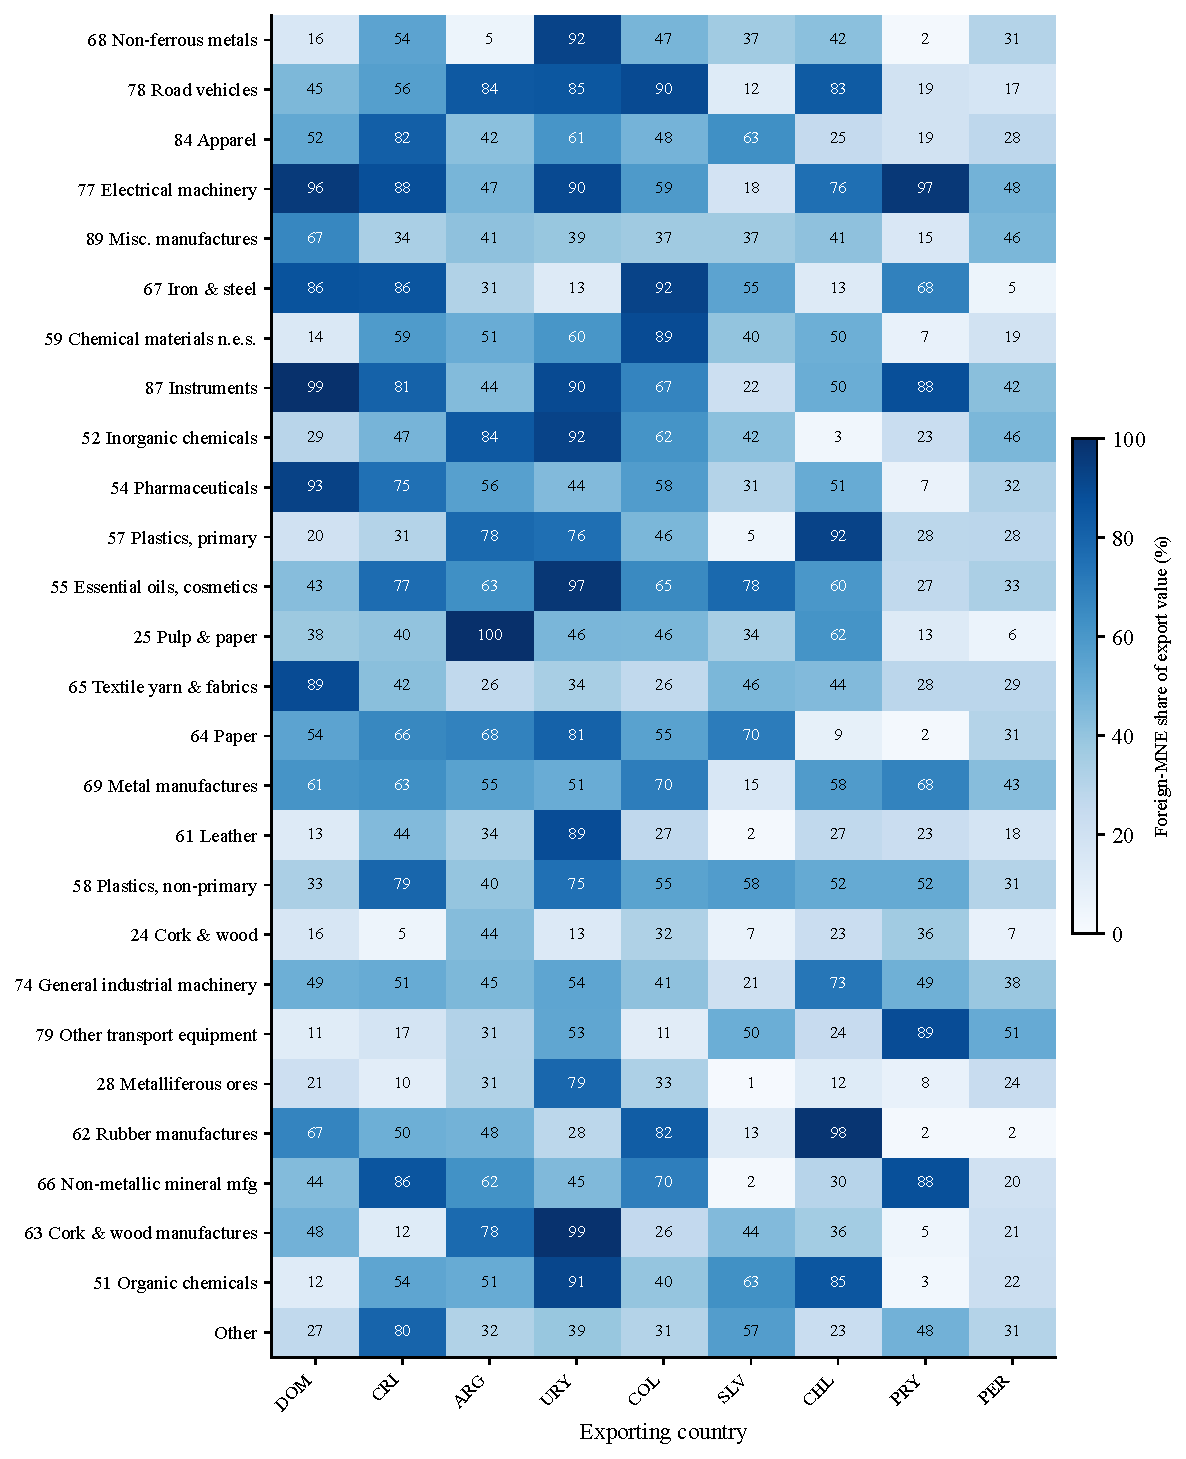
\includegraphics[width=0.95\textwidth,height=0.8\textheight,keepaspectratio]{figures/manufacturing/fig_wp2_origin_x_sitc2.pdf}%
  \caption{Manufacturing: Foreign-Multinational Share of Export Value, by Exporting Country and SITC Division}%
  \label{fig:sc_sitc2_hm_manufacturing}%
  \par\vspace{2pt}%
  \parbox{0.92\textwidth}{\footnotesize %
  \textit{Notes:} Percent of each group's export value in each country shipped by foreign MNEs. SITC Rev.\,3 divisions; HS6 products without an SITC correspondence are excluded.\\[3pt]%
  \textit{Source:} Authors' calculations based on customs data matched to Orbis and Dun \& Bradstreet.}%
  \end{figure}
% ---- Table: Manufacturing: Exports by Exporting Country and SITC Division
\begin{table}[H]\centering\footnotesize%
  \caption{Manufacturing: Exports by Exporting Country and SITC Division}%
  \label{tab:sc_sitc2_ht_manufacturing}%
  \adjustbox{max width=\textwidth, max totalheight=0.8\textheight}{\begin{tabular}{lrrrrrrrrrr}
\toprule
Sub-sector & ARG & CHL & COL & CRI & DOM & PER & PRY & SLV & URY & All \\
\midrule
\multicolumn{11}{l}{\textit{Panel A: composition of the origin's exports, \% (columns sum to 100)}} \\
68 Non-ferrous metals & 3.6 & 63.0 & 0.7 & 1.2 & 0.5 & 43.4 & 0.6 & 1.0 & 0.4 & 23.7 \\
78 Road vehicles & 35.2 & 0.7 & 6.0 & 0.5 & 0.3 & 0.6 & 0.4 & 0.2 & 8.4 & 10.2 \\
84 Apparel & 0.3 & 0.1 & 6.0 & 1.7 & 13.8 & 14.2 & 5.2 & 50.2 & 1.5 & 6.4 \\
77 Electrical machinery & 1.0 & 0.4 & 5.4 & 22.5 & 13.8 & 0.6 & 15.5 & 6.0 & 2.8 & 4.2 \\
89 Misc. manufactures & 1.8 & 0.5 & 4.9 & 12.3 & 10.2 & 3.6 & 8.7 & 7.7 & 8.7 & 3.9 \\
67 Iron \& steel & 5.0 & 1.1 & 8.7 & 2.4 & 6.3 & 1.9 & 0.5 & 3.9 & 2.7 & 3.7 \\
59 Chemical materials n.e.s. & 9.3 & 0.5 & 5.5 & 2.4 & 0.3 & 0.9 & 3.7 & 0.3 & 4.6 & 3.7 \\
87 Instruments & 0.6 & 0.1 & 0.8 & 26.9 & 19.0 & 0.2 & 1.4 & 0.1 & 0.4 & 3.3 \\
52 Inorganic chemicals & 1.6 & 6.6 & 1.3 & 0.3 & 0.2 & 3.9 & 0.4 & 0.1 & 0.7 & 2.9 \\
54 Pharmaceuticals & 4.4 & 0.5 & 4.7 & 4.0 & 4.1 & 0.6 & 4.8 & 3.2 & 5.3 & 2.8 \\
57 Plastics, primary & 3.3 & 0.3 & 10.9 & 0.4 & 0.9 & 0.8 & 1.5 & 0.5 & 2.0 & 2.6 \\
55 Essential oils, cosmetics & 3.9 & 0.2 & 7.2 & 1.1 & 1.8 & 2.0 & 2.4 & 1.6 & 3.3 & 2.6 \\
25 Pulp \& paper & 0.6 & 8.3 & 0.0 & 0.2 & 0.3 & 0.0 & 0.1 & 0.2 & 0.2 & 2.6 \\
65 Textile yarn \& fabrics & 0.8 & 0.2 & 3.9 & 1.0 & 7.5 & 4.4 & 10.8 & 7.8 & 1.7 & 2.3 \\
64 Paper & 1.5 & 1.8 & 3.8 & 1.8 & 1.2 & 1.9 & 2.6 & 6.3 & 3.2 & 2.3 \\
69 Metal manufactures & 1.7 & 1.3 & 4.0 & 2.0 & 1.2 & 2.1 & 1.2 & 1.4 & 0.3 & 1.9 \\
61 Leather & 3.9 & 0.1 & 1.5 & 0.1 & 0.2 & 0.2 & 12.7 & 0.1 & 11.7 & 1.7 \\
58 Plastics, non-primary & 1.2 & 0.6 & 3.5 & 2.3 & 1.6 & 3.1 & 1.0 & 1.4 & 2.9 & 1.7 \\
24 Cork \& wood & 0.4 & 3.1 & 0.3 & 0.7 & 0.0 & 1.4 & 5.8 & 0.1 & 10.1 & 1.6 \\
74 General industrial machinery & 3.5 & 0.6 & 2.0 & 0.8 & 0.7 & 1.0 & 0.6 & 0.4 & 0.8 & 1.6 \\
79 Other transport equipment & 4.6 & 0.3 & 0.5 & 0.1 & 0.1 & 0.3 & 2.8 & 0.0 & 0.9 & 1.4 \\
28 Metalliferous ores & 0.0 & 1.3 & 3.9 & 1.2 & 1.9 & 0.8 & 5.6 & 0.8 & 0.6 & 1.3 \\
62 Rubber manufactures & 1.3 & 1.0 & 1.0 & 4.2 & 0.2 & 1.0 & 0.3 & 0.0 & 4.0 & 1.3 \\
66 Non-metallic mineral mfg & 0.6 & 0.2 & 3.4 & 1.9 & 0.5 & 2.5 & 1.6 & 1.0 & 0.4 & 1.2 \\
63 Cork \& wood manufactures & 0.4 & 2.8 & 0.2 & 0.4 & 0.1 & 0.3 & 1.7 & 0.1 & 3.1 & 1.1 \\
51 Organic chemicals & 2.2 & 0.7 & 1.6 & 0.1 & 0.5 & 0.3 & 0.5 & 0.1 & 0.6 & 1.0 \\
72 Specialised machinery & 1.2 & 0.7 & 1.2 & 0.6 & 0.5 & 1.7 & 1.1 & 0.5 & 0.5 & 1.0 \\
26 Textile fibres & 1.5 & 0.1 & 0.1 & 0.0 & 0.5 & 1.6 & 1.2 & 0.2 & 10.6 & 0.9 \\
56 Fertilisers & 0.3 & 1.8 & 1.0 & 0.6 & 0.6 & 0.3 & 0.1 & 0.5 & 0.9 & 0.9 \\
53 Dyeing materials & 0.7 & 0.1 & 1.4 & 1.3 & 0.4 & 2.0 & 0.4 & 1.0 & 1.8 & 0.8 \\
71 Power machinery & 2.1 & 0.2 & 0.7 & 0.2 & 0.5 & 0.6 & 0.3 & 0.1 & 0.2 & 0.8 \\
85 Footwear & 0.1 & 0.0 & 0.4 & 0.0 & 7.2 & 0.3 & 1.9 & 1.1 & 0.1 & 0.6 \\
82 Furniture & 0.2 & 0.0 & 1.2 & 0.6 & 0.3 & 0.3 & 1.1 & 1.1 & 3.8 & 0.5 \\
Other & 1.4 & 0.8 & 2.3 & 4.0 & 2.6 & 1.0 & 1.4 & 0.7 & 1.1 & 1.5 \\
All sub-sectors & 100.0 & 100.0 & 100.0 & 100.0 & 100.0 & 100.0 & 100.0 & 100.0 & 100.0 & 100.0 \\
\midrule
\multicolumn{11}{l}{\textit{Panel B: foreign-MNE share of export value, \%}} \\
68 Non-ferrous metals & 5.1 & 42.1 & 46.9 & 54.5 & 15.6 & 30.6 & 1.8 & 36.6 & 92.2 & 38.6 \\
78 Road vehicles & 84.3 & 83.4 & 89.8 & 56.5 & 45.5 & 16.9 & 18.9 & 12.3 & 85.1 & 84.0 \\
84 Apparel & 41.9 & 25.0 & 47.6 & 81.7 & 52.5 & 27.7 & 19.0 & 63.1 & 60.6 & 51.5 \\
77 Electrical machinery & 46.6 & 75.8 & 58.7 & 87.9 & 96.0 & 47.8 & 96.7 & 18.1 & 90.1 & 74.7 \\
89 Misc. manufactures & 41.2 & 41.4 & 36.9 & 33.8 & 66.7 & 45.9 & 15.2 & 36.8 & 38.7 & 41.0 \\
67 Iron \& steel & 31.4 & 12.7 & 92.3 & 85.8 & 86.4 & 5.3 & 68.5 & 54.6 & 12.8 & 55.9 \\
59 Chemical materials n.e.s. & 50.7 & 49.6 & 89.2 & 58.5 & 14.5 & 18.8 & 7.2 & 40.1 & 60.2 & 57.6 \\
87 Instruments & 43.8 & 50.2 & 67.4 & 80.6 & 99.5 & 42.2 & 88.2 & 21.6 & 89.8 & 83.2 \\
52 Inorganic chemicals & 84.3 & 3.3 & 61.6 & 47.3 & 29.1 & 45.7 & 23.2 & 41.9 & 92.3 & 24.7 \\
54 Pharmaceuticals & 56.2 & 51.0 & 57.7 & 75.1 & 92.6 & 31.9 & 6.5 & 30.8 & 44.3 & 56.8 \\
57 Plastics, primary & 77.9 & 92.4 & 46.0 & 30.5 & 19.6 & 28.2 & 28.0 & 4.9 & 75.7 & 56.4 \\
55 Essential oils, cosmetics & 63.2 & 60.1 & 65.3 & 76.8 & 43.0 & 33.2 & 26.6 & 77.8 & 97.2 & 62.6 \\
25 Pulp \& paper & 100.0 & 61.7 & 46.0 & 40.5 & 37.6 & 6.1 & 13.1 & 34.3 & 46.1 & 63.5 \\
65 Textile yarn \& fabrics & 26.4 & 44.2 & 26.3 & 42.3 & 89.3 & 28.5 & 28.1 & 46.0 & 34.1 & 41.8 \\
64 Paper & 68.3 & 8.5 & 55.3 & 66.1 & 54.4 & 30.8 & 1.8 & 70.4 & 80.5 & 48.7 \\
69 Metal manufactures & 55.2 & 57.9 & 69.9 & 63.2 & 61.0 & 43.1 & 67.8 & 15.5 & 50.6 & 57.5 \\
61 Leather & 33.7 & 26.5 & 26.7 & 44.2 & 13.0 & 17.5 & 22.9 & 1.9 & 89.0 & 42.0 \\
58 Plastics, non-primary & 39.7 & 51.6 & 54.9 & 79.1 & 33.3 & 30.7 & 51.7 & 57.5 & 75.1 & 49.8 \\
24 Cork \& wood & 43.6 & 22.7 & 32.3 & 5.0 & 16.0 & 7.1 & 36.4 & 6.9 & 13.4 & 20.9 \\
74 General industrial machinery & 45.4 & 73.0 & 41.1 & 50.8 & 49.3 & 38.3 & 49.2 & 20.9 & 53.6 & 47.2 \\
79 Other transport equipment & 31.2 & 24.3 & 11.2 & 17.2 & 11.4 & 51.4 & 88.9 & 50.0 & 53.5 & 31.8 \\
28 Metalliferous ores & 31.3 & 12.5 & 32.7 & 10.3 & 21.2 & 23.8 & 7.6 & 1.1 & 78.7 & 21.9 \\
62 Rubber manufactures & 47.8 & 97.8 & 82.4 & 49.5 & 67.5 & 1.7 & 1.6 & 13.0 & 28.0 & 57.1 \\
66 Non-metallic mineral mfg & 62.3 & 29.5 & 69.7 & 85.9 & 44.1 & 19.9 & 87.8 & 2.1 & 44.9 & 53.7 \\
63 Cork \& wood manufactures & 77.6 & 35.6 & 25.9 & 12.4 & 48.2 & 21.5 & 4.5 & 44.3 & 98.9 & 42.2 \\
51 Organic chemicals & 51.0 & 85.2 & 39.5 & 53.7 & 11.7 & 22.5 & 2.8 & 62.8 & 91.2 & 53.6 \\
72 Specialised machinery & 35.4 & 58.4 & 37.5 & 43.5 & 57.4 & 32.1 & 12.2 & 37.4 & 51.2 & 41.0 \\
26 Textile fibres & 50.0 & 52.6 & 69.5 & 71.5 & 52.6 & 53.5 & 9.8 & 12.4 & 49.9 & 49.9 \\
56 Fertilisers & 25.5 & 1.8 & 54.0 & 82.3 & 0.4 & 72.6 & 33.2 & 93.5 & 1.5 & 21.6 \\
53 Dyeing materials & 38.2 & 63.3 & 28.8 & 76.4 & 46.5 & 40.8 & 37.3 & 84.0 & 96.3 & 49.2 \\
71 Power machinery & 78.9 & 72.3 & 38.0 & 12.7 & 71.8 & 16.4 & 56.1 & 26.8 & 7.6 & 66.1 \\
85 Footwear & 44.0 & 55.3 & 24.2 & 15.9 & 64.4 & 15.6 & 84.5 & 6.4 & 42.7 & 50.1 \\
82 Furniture & 30.7 & 24.3 & 19.5 & 61.7 & 28.0 & 10.9 & 4.3 & 30.7 & 90.5 & 40.3 \\
Other & 31.5 & 23.3 & 30.8 & 80.1 & 26.6 & 30.6 & 48.2 & 57.1 & 39.0 & 40.4 \\
All sub-sectors & 60.4 & 40.3 & 57.4 & 70.2 & 73.2 & 30.6 & 37.9 & 52.4 & 60.2 & 51.7 \\
\bottomrule
\end{tabular}
}%
  \par\vspace{3pt}%
  \begin{minipage}{0.95\textwidth}\footnotesize %
  \textit{Notes:} Panel A: composition of each country's exports in the sector (rows add to 100). Panel B: percent of each cell's export value shipped by foreign MNEs. SITC Rev.\,3 divisions; HS6 products without an SITC correspondence are excluded.\\[3pt]%
  \textit{Source:} Authors' calculations based on customs data matched to Orbis and Dun \& Bradstreet.%
  \end{minipage}%
  \end{table}
% ---- Table: Manufacturing: Exports by SITC Division and Parent Country
\begin{table}[H]\centering\footnotesize%
  \caption{Manufacturing: Exports by SITC Division and Parent Country}%
  \label{tab:sc_sitc2_par_manufacturing}%
  \adjustbox{max width=\textwidth, max totalheight=0.8\textheight}{\begin{tabular}{lrrrrrrrrrrrr}
\toprule
SITC Rev.\,3 division & USA & GBR & DEU & JPN & PAN & CAN & NLD & FRA & BRA & MEX & Other & Domestic \\
\midrule
68 Non-ferrous metals & 2.2 & 21.9 & 0.0 & 0.0 & 0.0 & 5.7 & 0.0 & 0.3 & 3.2 & 0.1 & 5.1 & 2.2 \\
78 Road vehicles & 8.6 & 0.1 & 26.4 & 24.7 & 0.0 & 0.3 & 10.8 & 9.8 & 0.9 & 0.0 & 2.4 & 0.7 \\
84 Apparel & 32.4 & 0.2 & 0.5 & 0.4 & 0.2 & 1.3 & 0.0 & 0.3 & 0.1 & 0.1 & 16.0 & 1.0 \\
77 Electrical machinery & 33.4 & 1.0 & 1.5 & 7.8 & 0.2 & 0.1 & 0.7 & 4.4 & 0.1 & 3.7 & 21.8 & 0.9 \\
89 Misc. manufactures & 10.5 & 5.5 & 2.3 & 2.0 & 1.7 & 4.3 & 0.3 & 0.9 & 1.1 & 1.0 & 11.4 & 18.9 \\
67 Iron \& steel & 0.4 & 0.2 & 0.2 & 0.0 & 3.2 & 0.0 & 5.1 & 0.1 & 2.5 & 2.1 & 42.0 & 7.9 \\
59 Chemical materials n.e.s. & 16.2 & 3.3 & 13.1 & 0.7 & 0.6 & 0.3 & 0.7 & 0.5 & 0.7 & 0.1 & 21.4 & 8.5 \\
87 Instruments & 52.9 & 5.2 & 9.2 & 2.4 & 0.1 & 0.2 & 0.3 & 0.6 & 0.0 & 0.0 & 12.2 & 0.8 \\
52 Inorganic chemicals & 7.2 & 0.1 & 1.4 & 0.0 & 0.1 & 1.6 & 0.8 & 0.1 & 1.6 & 0.0 & 11.6 & 30.7 \\
54 Pharmaceuticals & 10.1 & 1.0 & 6.4 & 0.0 & 1.0 & 0.2 & 0.2 & 2.3 & 2.0 & 0.2 & 33.5 & 6.7 \\
57 Plastics, primary & 16.5 & 0.1 & 0.9 & 0.9 & 0.8 & 0.3 & 3.7 & 0.7 & 3.6 & 20.7 & 8.3 & 5.2 \\
55 Essential oils, cosmetics & 14.0 & 18.3 & 4.1 & 2.1 & 2.9 & 0.1 & 0.3 & 0.6 & 5.0 & 0.4 & 15.0 & 11.8 \\
25 Pulp \& paper & 0.1 & 0.0 & 0.0 & 0.0 & 56.5 & 0.0 & 0.0 & 0.0 & 0.0 & 0.0 & 6.8 & 35.1 \\
65 Textile yarn \& fabrics & 17.6 & 1.7 & 0.5 & 1.6 & 1.0 & 3.0 & 0.1 & 0.3 & 1.1 & 0.3 & 14.6 & 7.8 \\
64 Paper & 21.3 & 0.7 & 0.1 & 0.0 & 2.5 & 0.0 & 0.0 & 0.0 & 0.1 & 0.6 & 23.4 & 22.6 \\
69 Metal manufactures & 12.4 & 1.1 & 1.0 & 2.8 & 1.1 & 0.6 & 2.6 & 2.1 & 0.5 & 1.5 & 31.8 & 4.7 \\
61 Leather & 1.0 & 0.0 & 2.1 & 0.0 & 0.0 & 0.0 & 1.7 & 0.1 & 3.1 & 0.2 & 33.7 & 12.8 \\
58 Plastics, non-primary & 10.2 & 5.6 & 0.2 & 0.7 & 3.4 & 0.4 & 1.9 & 0.9 & 0.8 & 2.8 & 22.9 & 11.0 \\
24 Cork \& wood & 1.5 & 0.8 & 0.0 & 5.3 & 0.0 & 0.1 & 0.0 & 0.2 & 0.0 & 0.2 & 12.8 & 21.1 \\
74 General industrial machinery & 9.9 & 3.4 & 2.6 & 1.7 & 0.4 & 1.9 & 1.9 & 1.5 & 1.4 & 0.7 & 21.6 & 10.4 \\
79 Other transport equipment & 0.3 & 0.1 & 0.1 & 0.9 & 0.0 & 0.1 & 0.0 & 0.1 & 0.6 & 0.0 & 29.6 & 29.2 \\
28 Metalliferous ores & 0.3 & 0.9 & 0.9 & 0.0 & 0.3 & 0.0 & 0.0 & 0.3 & 1.3 & 0.1 & 17.7 & 3.2 \\
62 Rubber manufactures & 29.6 & 0.3 & 1.3 & 12.5 & 0.0 & 0.1 & 0.3 & 3.0 & 0.1 & 0.0 & 10.0 & 1.1 \\
66 Non-metallic mineral mfg & 13.9 & 2.5 & 2.0 & 0.2 & 8.7 & 0.0 & 3.0 & 2.6 & 0.6 & 2.4 & 17.7 & 4.5 \\
63 Cork \& wood manufactures & 4.5 & 0.1 & 0.3 & 0.0 & 0.2 & 2.9 & 0.0 & 0.5 & 0.3 & 0.1 & 33.1 & 41.3 \\
51 Organic chemicals & 11.5 & 5.9 & 2.4 & 0.4 & 0.6 & 14.6 & 1.1 & 0.2 & 0.3 & 0.1 & 16.4 & 8.0 \\
72 Specialised machinery & 5.9 & 2.6 & 1.7 & 0.7 & 0.4 & 2.9 & 0.6 & 1.4 & 0.3 & 0.4 & 24.1 & 7.0 \\
26 Textile fibres & 0.9 & 6.7 & 0.2 & 0.0 & 4.7 & 0.0 & 0.0 & 11.6 & 0.0 & 0.0 & 25.7 & 4.2 \\
56 Fertilisers & 0.2 & 0.1 & 0.0 & 0.0 & 3.0 & 0.1 & 0.4 & 0.0 & 0.0 & 0.0 & 17.8 & 34.5 \\
53 Dyeing materials & 12.2 & 0.2 & 2.3 & 1.9 & 0.1 & 0.1 & 4.0 & 0.2 & 1.0 & 0.1 & 27.1 & 6.9 \\
71 Power machinery & 20.1 & 1.7 & 9.0 & 0.4 & 0.5 & 4.2 & 6.9 & 1.7 & 4.2 & 0.3 & 17.1 & 2.7 \\
85 Footwear & 29.3 & 0.1 & 1.0 & 3.7 & 0.0 & 0.0 & 0.0 & 0.6 & 5.6 & 0.0 & 9.8 & 1.2 \\
82 Furniture & 2.5 & 0.3 & 5.5 & 0.6 & 0.1 & 0.0 & 1.1 & 5.3 & 0.1 & 2.2 & 22.6 & 2.0 \\
Other & 16.7 & 3.2 & 1.1 & 0.7 & 0.7 & 0.2 & 1.1 & 0.6 & 0.3 & 1.4 & 14.4 & 4.0 \\
\bottomrule
\end{tabular}
}%
  \par\vspace{3pt}%
  \begin{minipage}{0.95\textwidth}\footnotesize %
  \textit{Notes:} Percent of each group's export value, by country of the ultimate parent of foreign MNEs; domestic MNEs shown for comparison. SITC Rev.\,3 divisions; HS6 products without an SITC correspondence are excluded.\\[3pt]%
  \textit{Source:} Authors' calculations based on customs data matched to Orbis and Dun \& Bradstreet.%
  \end{minipage}%
  \end{table}

\subsection{By NAICS Industry}
% ---- Table: Manufacturing: Exports and Multinational Shares, by NAICS Industry
\begin{table}[H]\centering\footnotesize%
  \caption{Manufacturing: Exports and Multinational Shares, by NAICS Industry}%
  \label{tab:sc_naics3_manufacturing}%
  \adjustbox{max width=\textwidth, max totalheight=0.8\textheight}{\begin{tabular}{@{}l r r r r l@{}}
\toprule
NAICS 3-digit (product-based) & Total exports (US\$bn/yr) & MNE exports (US\$bn/yr) & Foreign (\%) & Domestic (\%) & Leading parents (share of foreign) \\
\midrule
331 Primary metals & 17.3 & 7.5 & 40.6 & 3.1 & GBR 0.48, CAN 0.13, ZAF 0.09 \\
325 Chemicals & 11.5 & 7.4 & 50.4 & 13.2 & USA 0.30, DEU 0.12, GBR 0.10 \\
336 Transport equipment & 9.7 & 8.0 & 78.5 & 3.8 & JPN 0.30, DEU 0.29, NLD 0.12 \\
315 Apparel & 4.4 & 2.3 & 51.4 & 0.9 & USA 0.73, CHE 0.04, CAN 0.03 \\
322 Paper & 2.9 & 2.5 & 55.7 & 31.3 & PAN 0.59, USA 0.14, CHL 0.09 \\
326 Plastics \& rubber & 3.4 & 2.0 & 50.9 & 8.8 & USA 0.36, JPN 0.08, CAN 0.08 \\
339 Misc. manufacturing & 3.8 & 3.0 & 71.3 & 7.8 & USA 0.59, DEU 0.13, GBR 0.11 \\
333 Machinery & 2.4 & 1.5 & 53.7 & 8.2 & USA 0.28, DEU 0.14, NLD 0.07 \\
334 Computers \& electronics & 2.2 & 1.5 & 66.9 & 2.2 & USA 0.79, DEU 0.03, JPN 0.03 \\
316 Leather & 2.0 & 1.1 & 45.8 & 9.5 & USA 0.19, BGR 0.13, CHL 0.12 \\
321 Wood products & 1.5 & 0.9 & 30.0 & 32.1 & BHS 0.25, JPN 0.13, USA 0.11 \\
335 Electrical equipment & 1.9 & 1.4 & 68.6 & 2.5 & IRL 0.29, USA 0.16, ITA 0.11 \\
313 Textile mills & 1.6 & 0.9 & 45.2 & 5.2 & USA 0.36, FRA 0.12, GBR 0.09 \\
332 Fabricated metals & 1.5 & 0.9 & 58.3 & 3.8 & USA 0.25, CYM 0.20, GBR 0.07 \\
910 & 1.0 & 0.3 & 23.8 & 2.8 & BGR 0.25, TUR 0.10, BRA 0.10 \\
327 Non-metallic minerals & 0.8 & 0.5 & 54.6 & 3.8 & USA 0.32, PAN 0.20, CYM 0.11 \\
314 Textile products & 0.4 & 0.2 & 33.2 & 3.6 & USA 0.36, PAN 0.16, GBR 0.12 \\
Other & 1.2 & 0.5 & 29.9 & 12.0 & USA 0.20, DNK 0.09, AUS 0.08 \\
\midrule
All & 69.7 & 42.2 & 52.0 & 7.8 & \\
\bottomrule
\end{tabular}
}%
  \par\vspace{3pt}%
  \begin{minipage}{0.95\textwidth}\footnotesize %
  \textit{Notes:} NAICS 3-digit industries assigned to HS6 products. Foreign and domestic: percent of the group's export value. Leading parents: the three largest parent countries and their share of the row's foreign-MNE exports. Values are annual averages in US\$ billion.\\[3pt]%
  \textit{Source:} Authors' calculations based on customs data matched to Orbis and Dun \& Bradstreet.%
  \end{minipage}%
  \end{table}
% ---- Figure: Manufacturing: Multinational Share of Export Value, by NAICS Industry
\begin{figure}[H]\centering%
  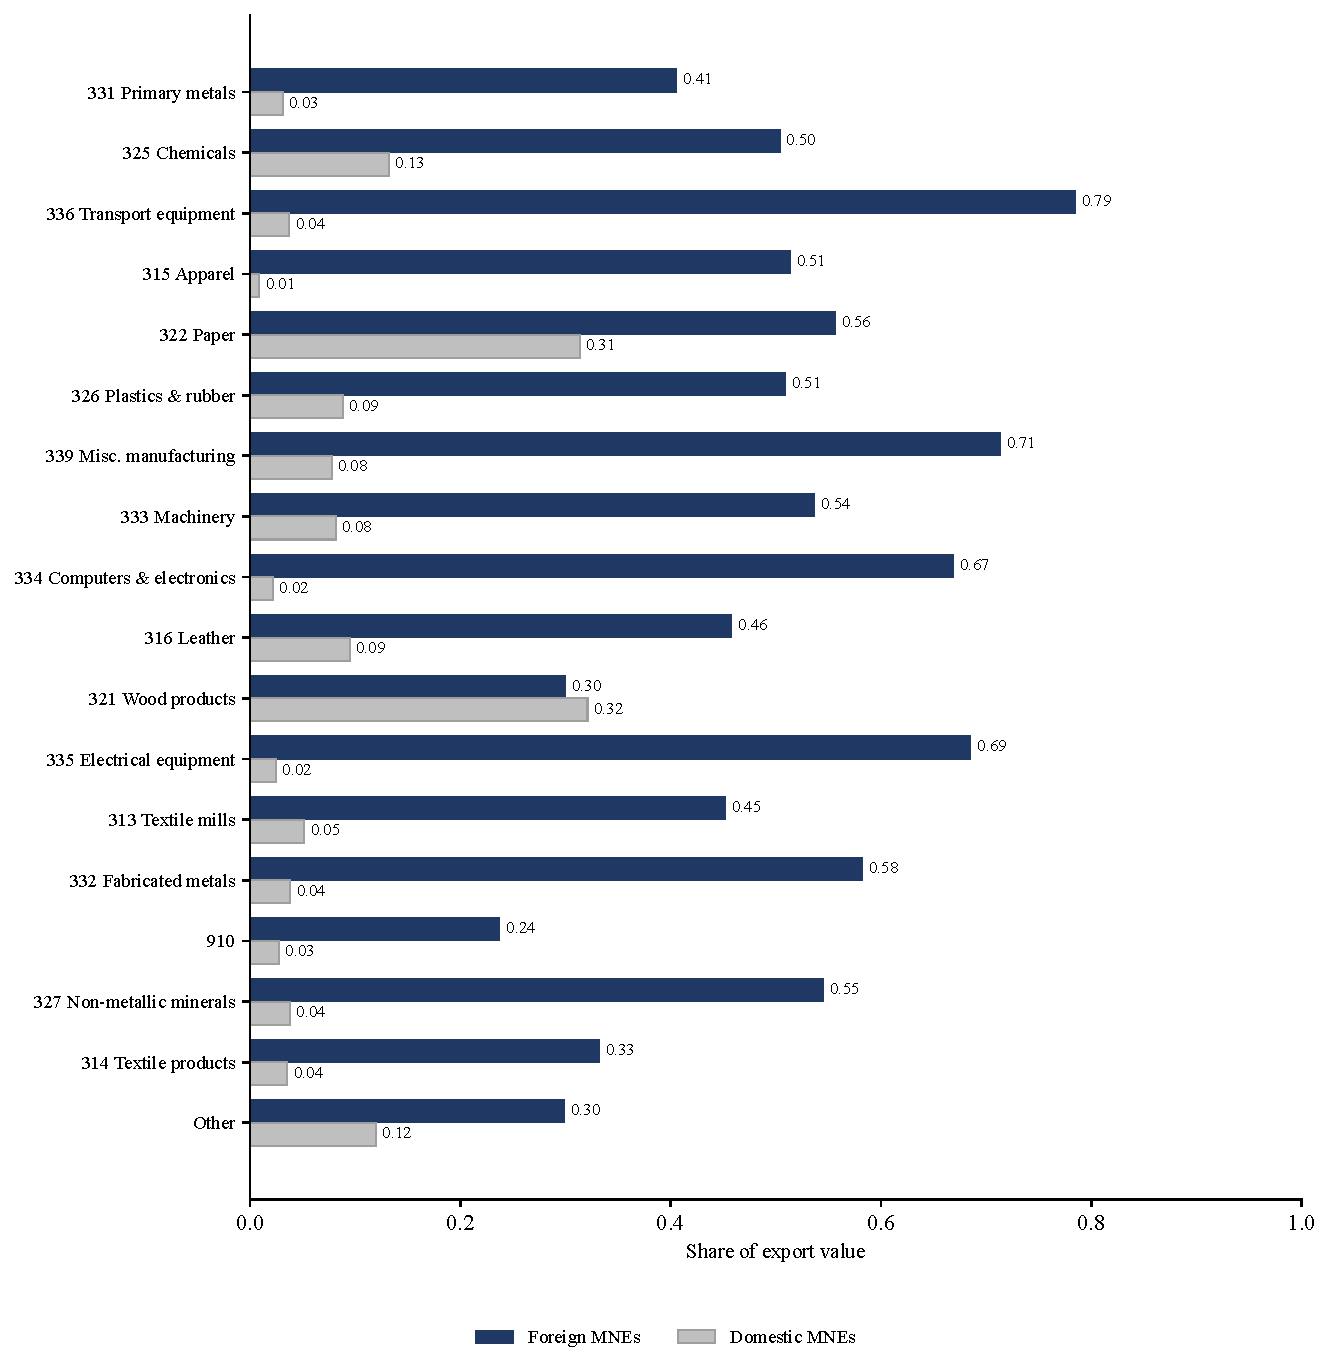
\includegraphics[width=0.9\textwidth,height=0.8\textheight,keepaspectratio]{figures/manufacturing/fig_wp2_naics3.pdf}%
  \caption{Manufacturing: Multinational Share of Export Value, by NAICS Industry}%
  \label{fig:sc_naics3_f_manufacturing}%
  \par\vspace{2pt}%
  \parbox{0.92\textwidth}{\footnotesize %
  \textit{Notes:} Shares of manufacturing export value (HS 28--97 excluding 71), all available years pooled. NAICS 3-digit industries assigned to HS6 products.\\[3pt]%
  \textit{Source:} Authors' calculations based on customs data matched to Orbis and Dun \& Bradstreet.}%
  \end{figure}
% ---- Figure: Manufacturing: Foreign-Multinational Share of Export Value, by Exporting Country and NAICS Industry
\begin{figure}[H]\centering%
  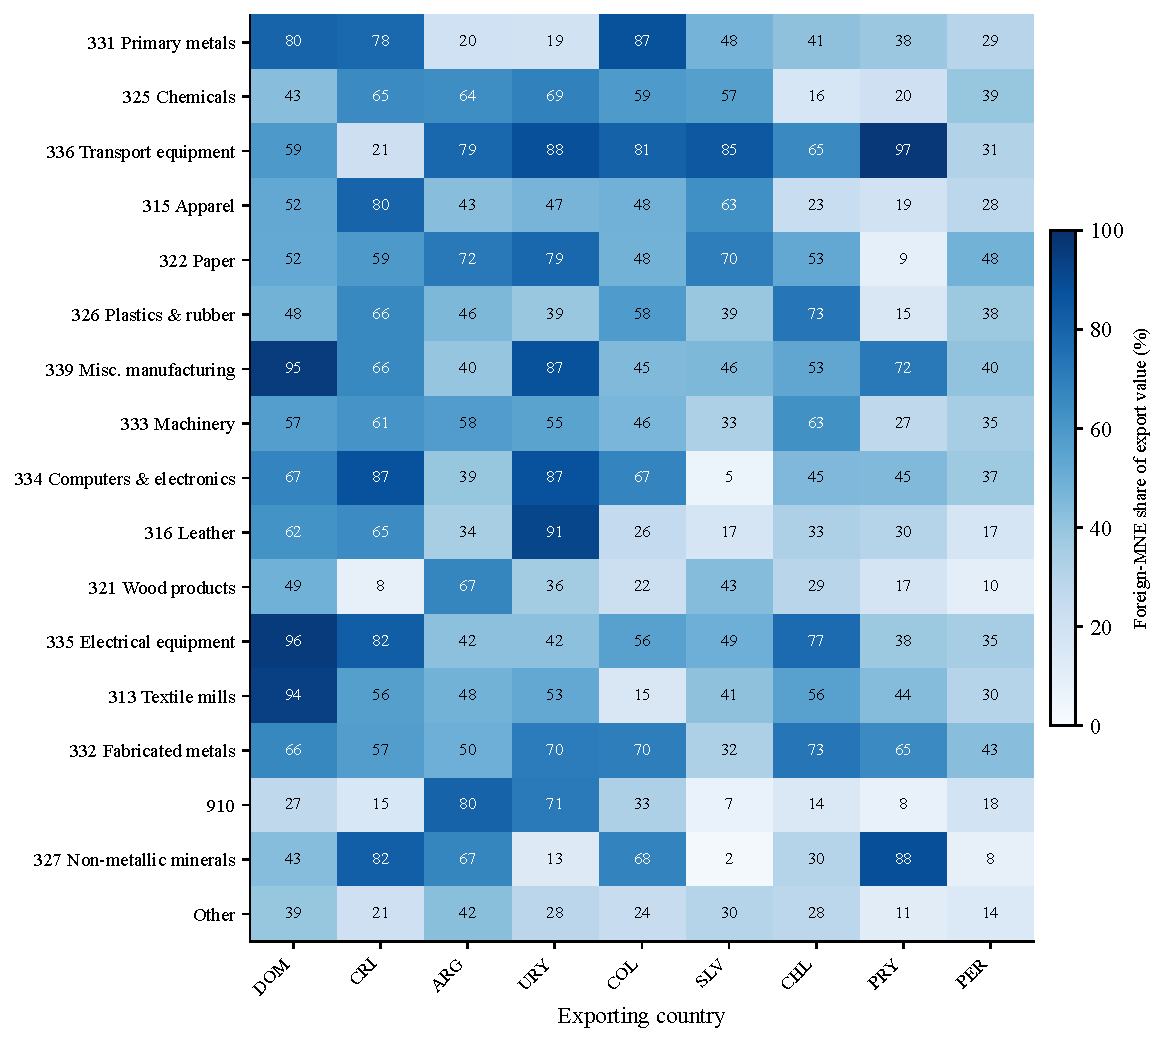
\includegraphics[width=0.95\textwidth,height=0.8\textheight,keepaspectratio]{figures/manufacturing/fig_wp2_origin_x_naics3.pdf}%
  \caption{Manufacturing: Foreign-Multinational Share of Export Value, by Exporting Country and NAICS Industry}%
  \label{fig:sc_naics3_hm_manufacturing}%
  \par\vspace{2pt}%
  \parbox{0.92\textwidth}{\footnotesize %
  \textit{Notes:} Percent of each group's export value in each country shipped by foreign MNEs. NAICS 3-digit industries assigned to HS6 products.\\[3pt]%
  \textit{Source:} Authors' calculations based on customs data matched to Orbis and Dun \& Bradstreet.}%
  \end{figure}
% ---- Table: Manufacturing: Exports by Exporting Country and NAICS Industry
\begin{table}[H]\centering\footnotesize%
  \caption{Manufacturing: Exports by Exporting Country and NAICS Industry}%
  \label{tab:sc_naics3_ht_manufacturing}%
  \adjustbox{max width=\textwidth, max totalheight=0.8\textheight}{\begin{tabular}{lrrrrrrrrrr}
\toprule
Sub-sector & ARG & CHL & COL & CRI & DOM & PER & PRY & SLV & URY & All \\
\midrule
\multicolumn{11}{l}{\textit{Panel A: composition of the origin's exports, \% (columns sum to 100)}} \\
331 Primary metals & 9.1 & 64.5 & 9.6 & 3.7 & 6.8 & 46.8 & 1.1 & 4.6 & 3.0 & 28.2 \\
325 Chemicals & 21.5 & 11.0 & 33.6 & 9.2 & 6.2 & 11.0 & 16.6 & 8.0 & 18.1 & 16.3 \\
336 Transport equipment & 41.9 & 1.0 & 6.5 & 0.4 & 0.5 & 1.0 & 18.3 & 0.9 & 10.5 & 11.9 \\
315 Apparel & 0.3 & 0.1 & 6.0 & 1.4 & 13.7 & 14.5 & 5.2 & 50.4 & 1.1 & 6.5 \\
322 Paper & 2.0 & 10.1 & 3.9 & 1.7 & 1.5 & 1.2 & 2.9 & 6.5 & 2.9 & 4.8 \\
326 Plastics \& rubber & 3.3 & 1.7 & 6.8 & 8.6 & 5.9 & 6.3 & 8.8 & 7.1 & 14.2 & 4.8 \\
339 Misc. manufacturing & 0.7 & 0.1 & 1.8 & 35.9 & 26.9 & 0.9 & 2.1 & 0.9 & 0.9 & 4.7 \\
333 Machinery & 6.5 & 1.4 & 4.0 & 2.4 & 1.1 & 2.8 & 2.2 & 1.0 & 2.4 & 3.2 \\
334 Computers \& electronics & 1.1 & 0.5 & 1.7 & 20.6 & 5.6 & 0.6 & 1.2 & 5.1 & 1.7 & 2.9 \\
316 Leather & 4.4 & 0.1 & 2.3 & 0.3 & 7.4 & 0.5 & 15.6 & 1.3 & 15.4 & 2.5 \\
321 Wood products & 0.6 & 5.9 & 0.3 & 0.6 & 0.1 & 1.8 & 3.2 & 0.1 & 10.7 & 2.5 \\
335 Electrical equipment & 1.4 & 0.5 & 5.4 & 6.9 & 11.5 & 1.1 & 0.8 & 0.7 & 0.6 & 2.5 \\
313 Textile mills & 1.3 & 0.2 & 2.4 & 0.6 & 6.4 & 4.7 & 3.3 & 5.6 & 9.2 & 2.2 \\
332 Fabricated metals & 2.7 & 1.1 & 4.1 & 2.2 & 1.3 & 2.0 & 1.3 & 1.8 & 0.5 & 2.1 \\
910 & 0.1 & 1.2 & 4.0 & 1.5 & 3.0 & 0.9 & 5.8 & 1.4 & 0.9 & 1.4 \\
327 Non-metallic minerals & 0.5 & 0.2 & 3.5 & 2.1 & 0.6 & 1.5 & 1.7 & 1.0 & 0.3 & 1.1 \\
314 Textile products & 0.2 & 0.0 & 1.3 & 0.4 & 0.4 & 0.8 & 7.9 & 1.7 & 1.3 & 0.6 \\
Other & 2.3 & 0.2 & 3.0 & 1.4 & 0.7 & 1.6 & 2.0 & 2.0 & 6.4 & 1.7 \\
All sub-sectors & 100.0 & 100.0 & 100.0 & 100.0 & 100.0 & 100.0 & 100.0 & 100.0 & 100.0 & 100.0 \\
\midrule
\multicolumn{11}{l}{\textit{Panel B: foreign-MNE share of export value, \%}} \\
331 Primary metals & 20.3 & 41.3 & 87.1 & 78.4 & 80.1 & 29.5 & 37.9 & 47.7 & 18.9 & 40.6 \\
325 Chemicals & 63.9 & 16.1 & 58.9 & 65.1 & 42.7 & 39.4 & 20.3 & 56.6 & 68.7 & 50.4 \\
336 Transport equipment & 78.7 & 65.4 & 80.6 & 21.2 & 59.4 & 31.4 & 96.8 & 84.7 & 87.7 & 78.5 \\
315 Apparel & 42.7 & 23.1 & 48.1 & 79.7 & 52.5 & 27.8 & 19.1 & 63.1 & 47.2 & 51.4 \\
322 Paper & 71.7 & 52.6 & 47.8 & 59.2 & 52.1 & 48.0 & 8.7 & 69.8 & 78.6 & 55.7 \\
326 Plastics \& rubber & 45.5 & 73.3 & 58.4 & 65.9 & 47.8 & 37.6 & 15.0 & 38.9 & 38.6 & 50.9 \\
339 Misc. manufacturing & 39.7 & 53.4 & 44.7 & 66.0 & 95.1 & 40.4 & 71.7 & 45.6 & 87.0 & 71.3 \\
333 Machinery & 57.7 & 62.8 & 46.4 & 61.2 & 56.9 & 35.1 & 27.2 & 32.7 & 55.1 & 53.7 \\
334 Computers \& electronics & 39.2 & 45.3 & 67.3 & 87.2 & 67.2 & 37.4 & 44.6 & 5.2 & 87.3 & 66.9 \\
316 Leather & 34.2 & 32.7 & 25.5 & 64.6 & 61.8 & 16.9 & 29.7 & 16.9 & 91.2 & 45.8 \\
321 Wood products & 67.0 & 29.0 & 21.7 & 7.8 & 48.7 & 9.6 & 17.4 & 43.4 & 35.6 & 30.0 \\
335 Electrical equipment & 41.6 & 77.1 & 55.6 & 82.3 & 95.6 & 34.8 & 37.6 & 49.3 & 41.6 & 68.6 \\
313 Textile mills & 47.7 & 55.5 & 15.1 & 56.4 & 93.5 & 29.8 & 43.7 & 41.1 & 52.6 & 45.2 \\
332 Fabricated metals & 49.5 & 73.0 & 69.8 & 57.4 & 66.2 & 42.9 & 65.1 & 32.5 & 70.4 & 58.3 \\
910 & 80.3 & 14.4 & 32.7 & 15.2 & 27.3 & 18.4 & 7.7 & 6.7 & 71.3 & 23.8 \\
327 Non-metallic minerals & 67.0 & 30.2 & 67.6 & 81.7 & 43.1 & 8.0 & 88.2 & 2.1 & 13.0 & 54.6 \\
314 Textile products & 31.1 & 46.1 & 30.6 & 37.3 & 13.5 & 46.3 & 21.3 & 40.3 & 30.3 & 33.2 \\
Other & 42.5 & 27.9 & 23.6 & 20.5 & 39.1 & 13.8 & 11.3 & 30.0 & 28.2 & 29.9 \\
All sub-sectors & 62.1 & 40.3 & 57.5 & 69.8 & 73.2 & 30.8 & 38.4 & 52.5 & 60.2 & 52.0 \\
\bottomrule
\end{tabular}
}%
  \par\vspace{3pt}%
  \begin{minipage}{0.95\textwidth}\footnotesize %
  \textit{Notes:} Panel A: composition of each country's exports in the sector (rows add to 100). Panel B: percent of each cell's export value shipped by foreign MNEs. NAICS 3-digit industries assigned to HS6 products.\\[3pt]%
  \textit{Source:} Authors' calculations based on customs data matched to Orbis and Dun \& Bradstreet.%
  \end{minipage}%
  \end{table}
% ---- Table: Manufacturing: Exports by NAICS Industry and Parent Country
\begin{table}[H]\centering\footnotesize%
  \caption{Manufacturing: Exports by NAICS Industry and Parent Country}%
  \label{tab:sc_naics3_par_manufacturing}%
  \adjustbox{max width=\textwidth, max totalheight=0.8\textheight}{\begin{tabular}{lrrrrrrrrrrrr}
\toprule
NAICS 3-digit (product-based) & USA & GBR & DEU & JPN & PAN & CAN & NLD & FRA & BRA & MEX & Other & Domestic \\
\midrule
331 Primary metals & 1.9 & 18.8 & 0.1 & 0.0 & 0.4 & 5.0 & 0.7 & 0.4 & 3.1 & 0.3 & 9.9 & 3.1 \\
325 Chemicals & 13.4 & 4.4 & 5.3 & 0.8 & 1.1 & 1.4 & 1.3 & 0.8 & 2.3 & 3.4 & 16.3 & 13.2 \\
336 Transport equipment & 7.3 & 0.2 & 22.4 & 23.3 & 0.0 & 0.2 & 9.4 & 8.6 & 0.8 & 0.0 & 6.4 & 3.8 \\
315 Apparel & 32.4 & 0.2 & 0.5 & 0.4 & 0.2 & 1.3 & 0.0 & 0.3 & 0.1 & 0.1 & 15.9 & 0.9 \\
322 Paper & 7.9 & 0.9 & 0.0 & 0.1 & 32.1 & 0.0 & 0.0 & 0.0 & 0.0 & 0.2 & 14.4 & 31.3 \\
326 Plastics \& rubber & 16.4 & 2.5 & 0.7 & 3.7 & 2.6 & 3.7 & 1.0 & 1.7 & 1.2 & 1.8 & 15.7 & 8.8 \\
339 Misc. manufacturing & 39.1 & 7.3 & 8.3 & 2.2 & 0.2 & 0.2 & 0.1 & 0.4 & 0.2 & 0.0 & 13.4 & 7.8 \\
333 Machinery & 13.1 & 2.8 & 6.6 & 2.3 & 0.4 & 2.4 & 3.4 & 1.5 & 1.9 & 0.5 & 18.8 & 8.2 \\
334 Computers \& electronics & 51.5 & 1.0 & 2.2 & 1.8 & 0.2 & 0.1 & 0.6 & 1.0 & 0.1 & 0.7 & 7.6 & 2.2 \\
316 Leather & 7.7 & 0.0 & 2.8 & 0.8 & 0.4 & 0.0 & 1.2 & 1.3 & 3.5 & 0.6 & 27.5 & 9.5 \\
321 Wood products & 3.0 & 0.5 & 0.1 & 3.4 & 0.1 & 1.4 & 0.0 & 0.3 & 0.1 & 0.1 & 20.8 & 32.1 \\
335 Electrical equipment & 10.0 & 1.5 & 0.8 & 3.8 & 0.6 & 0.5 & 1.0 & 6.5 & 0.1 & 7.0 & 36.6 & 2.5 \\
313 Textile mills & 15.0 & 3.6 & 0.6 & 1.5 & 2.3 & 3.3 & 0.0 & 4.8 & 1.2 & 0.3 & 12.5 & 5.2 \\
332 Fabricated metals & 11.1 & 2.9 & 0.9 & 2.6 & 0.6 & 1.3 & 2.8 & 1.3 & 0.4 & 0.6 & 33.7 & 3.8 \\
910 & 0.8 & 0.8 & 1.1 & 0.0 & 0.5 & 0.0 & 0.0 & 0.1 & 1.2 & 0.1 & 19.1 & 2.8 \\
327 Non-metallic minerals & 15.6 & 2.8 & 2.3 & 0.3 & 9.7 & 0.0 & 2.5 & 2.8 & 0.3 & 2.3 & 16.0 & 3.8 \\
314 Textile products & 7.1 & 2.3 & 0.2 & 0.2 & 3.2 & 0.0 & 0.9 & 1.8 & 0.1 & 0.1 & 17.3 & 3.6 \\
Other & 4.0 & 1.3 & 1.1 & 0.5 & 0.1 & 0.1 & 0.7 & 0.3 & 0.1 & 0.5 & 21.2 & 12.0 \\
\bottomrule
\end{tabular}
}%
  \par\vspace{3pt}%
  \begin{minipage}{0.95\textwidth}\footnotesize %
  \textit{Notes:} Percent of each group's export value, by country of the ultimate parent of foreign MNEs; domestic MNEs shown for comparison. NAICS 3-digit industries assigned to HS6 products.\\[3pt]%
  \textit{Source:} Authors' calculations based on customs data matched to Orbis and Dun \& Bradstreet.%
  \end{minipage}%
  \end{table}

\subsection{By Technology Class}
% ---- Table: Manufacturing: Exports and Multinational Shares, by Technology Class
\begin{table}[H]\centering\footnotesize%
  \caption{Manufacturing: Exports and Multinational Shares, by Technology Class}%
  \label{tab:sc_lall2000_category_manufacturing}%
  \adjustbox{max width=\textwidth, max totalheight=0.8\textheight}{\begin{tabular}{@{}l r r r r l@{}}
\toprule
Lall (2000) category & Total exports (US\$bn/yr) & MNE exports (US\$bn/yr) & Foreign (\%) & Domestic (\%) & Leading parents (share of foreign) \\
\midrule
Primary products & 15.6 & 6.3 & 38.5 & 2.7 & GBR 0.57, CAN 0.15, BRA 0.08 \\
Medium technology manufactures: process & 10.8 & 6.8 & 54.5 & 9.5 & USA 0.22, ZAF 0.13, GBR 0.10 \\
Low technology manufactures: textile, garment and footwear & 8.1 & 4.2 & 48.0 & 4.1 & USA 0.59, URY 0.04, CAN 0.03 \\
Medium technology manufactures: automotive & 8.5 & 7.2 & 84.3 & 0.6 & DEU 0.32, JPN 0.30, NLD 0.13 \\
Medium technology manufactures: engineering & 7.3 & 5.2 & 67.1 & 3.9 & USA 0.42, IRL 0.10, DEU 0.08 \\
Low technology manufactures: other products & 6.3 & 4.1 & 52.1 & 12.6 & USA 0.29, PAN 0.09, GBR 0.06 \\
Resource-based manufactures: agro-based & 4.8 & 3.4 & 46.8 & 27.8 & PAN 0.44, USA 0.16, CHL 0.07 \\
Resource-based manufactures: other & 4.7 & 2.4 & 33.0 & 16.6 & USA 0.25, CHE 0.09, DEU 0.08 \\
High technology manufactures: other & 3.2 & 2.2 & 52.7 & 14.2 & USA 0.20, CHL 0.15, DEU 0.10 \\
High technology manufactures: electronic and electrical & 2.2 & 1.4 & 62.7 & 1.1 & USA 0.76, JPN 0.05, DEU 0.03 \\
Unclassified products & 0.4 & 0.2 & 33.0 & 14.1 & USA 0.41, BGR 0.20, ESP 0.07 \\
\midrule
All & 71.7 & 43.3 & 51.7 & 7.8 & \\
\bottomrule
\end{tabular}
}%
  \par\vspace{3pt}%
  \begin{minipage}{0.95\textwidth}\footnotesize %
  \textit{Notes:} Lall (2000) technology classes. Foreign and domestic: percent of the group's export value. Leading parents: the three largest parent countries and their share of the row's foreign-MNE exports. Values are annual averages in US\$ billion.\\[3pt]%
  \textit{Source:} Authors' calculations based on customs data matched to Orbis and Dun \& Bradstreet.%
  \end{minipage}%
  \end{table}
% ---- Figure: Manufacturing: Multinational Share of Export Value, by Technology Class
\begin{figure}[H]\centering%
  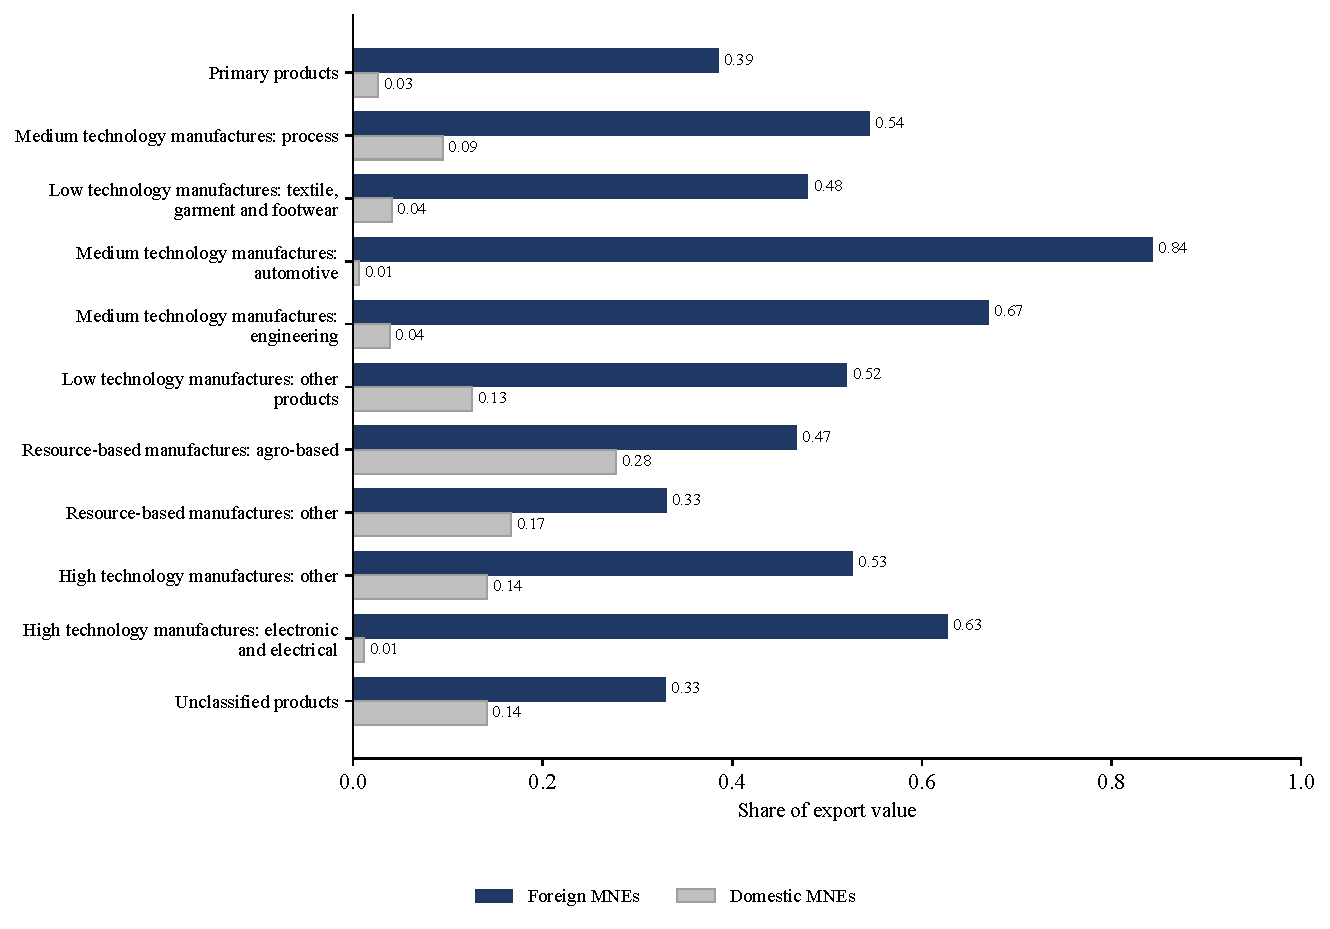
\includegraphics[width=0.9\textwidth,height=0.8\textheight,keepaspectratio]{figures/manufacturing/fig_wp2_lall2000_category.pdf}%
  \caption{Manufacturing: Multinational Share of Export Value, by Technology Class}%
  \label{fig:sc_lall2000_category_f_manufacturing}%
  \par\vspace{2pt}%
  \parbox{0.92\textwidth}{\footnotesize %
  \textit{Notes:} Shares of manufacturing export value (HS 28--97 excluding 71), all available years pooled. Lall (2000) technology classes.\\[3pt]%
  \textit{Source:} Authors' calculations based on customs data matched to Orbis and Dun \& Bradstreet.}%
  \end{figure}
% ---- Figure: Manufacturing: Foreign-Multinational Share of Export Value, by Exporting Country and Technology Class
\begin{figure}[H]\centering%
  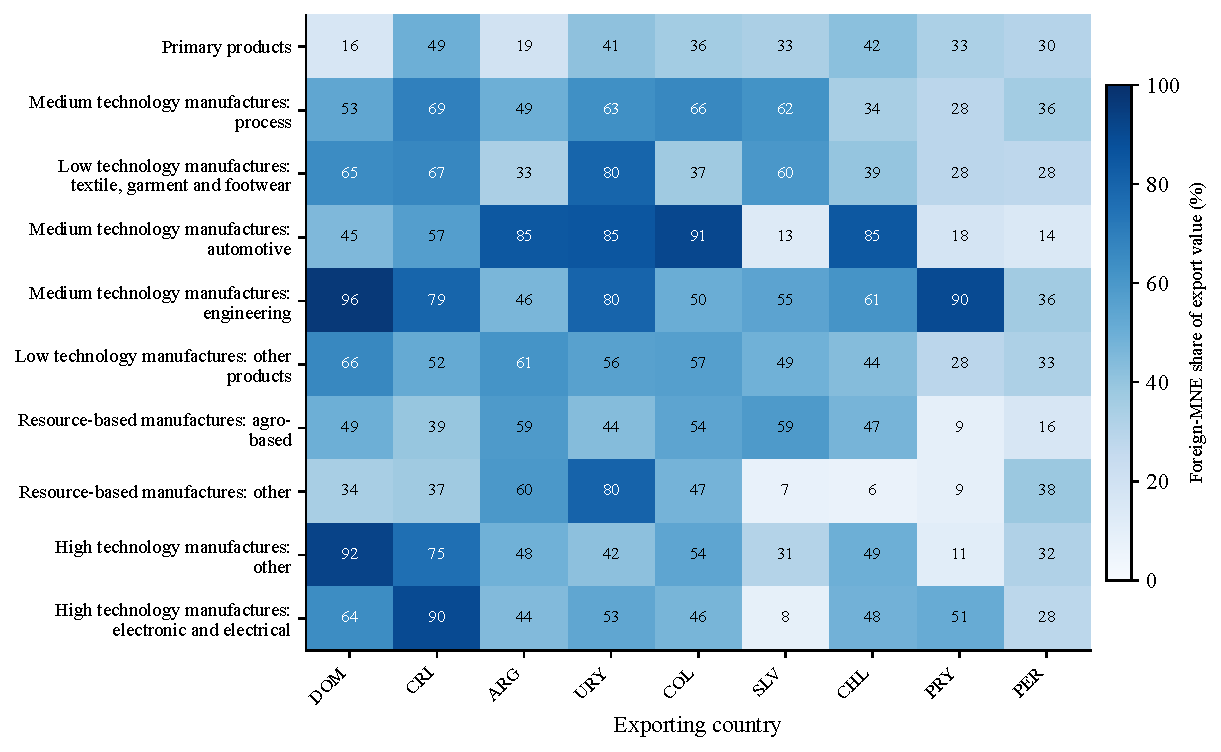
\includegraphics[width=0.95\textwidth,height=0.8\textheight,keepaspectratio]{figures/manufacturing/fig_wp2_origin_x_lall2000_category.pdf}%
  \caption{Manufacturing: Foreign-Multinational Share of Export Value, by Exporting Country and Technology Class}%
  \label{fig:sc_lall2000_category_hm_manufacturing}%
  \par\vspace{2pt}%
  \parbox{0.92\textwidth}{\footnotesize %
  \textit{Notes:} Percent of each group's export value in each country shipped by foreign MNEs. Lall (2000) technology classes.\\[3pt]%
  \textit{Source:} Authors' calculations based on customs data matched to Orbis and Dun \& Bradstreet.}%
  \end{figure}
% ---- Table: Manufacturing: Exports by Exporting Country and Technology Class
\begin{table}[H]\centering\footnotesize%
  \caption{Manufacturing: Exports by Exporting Country and Technology Class}%
  \label{tab:sc_lall2000_category_ht_manufacturing}%
  \adjustbox{max width=\textwidth, max totalheight=0.8\textheight}{\begin{tabular}{lrrrrrrrrrr}
\toprule
Sub-sector & ARG & CHL & COL & CRI & DOM & PER & PRY & SLV & URY & All \\
\midrule
\multicolumn{11}{l}{\textit{Panel A: composition of the origin's exports, \% (columns sum to 100)}} \\
Primary products & 5.3 & 64.4 & 1.2 & 1.4 & 0.7 & 44.7 & 5.2 & 1.1 & 15.8 & 25.2 \\
Medium technology manufactures: process & 21.0 & 4.9 & 37.4 & 8.2 & 8.9 & 8.2 & 9.2 & 6.5 & 16.3 & 14.5 \\
Low technology manufactures: textile, garment and footwear & 5.1 & 0.3 & 11.9 & 2.9 & 28.8 & 19.0 & 29.8 & 58.5 & 15.0 & 11.0 \\
Medium technology manufactures: automotive & 35.0 & 0.7 & 5.9 & 0.4 & 0.3 & 0.6 & 0.4 & 0.2 & 8.3 & 10.1 \\
Medium technology manufactures: engineering & 9.2 & 2.1 & 8.1 & 36.0 & 30.5 & 3.7 & 21.2 & 2.2 & 4.7 & 9.1 \\
Low technology manufactures: other products & 5.2 & 2.4 & 13.0 & 19.2 & 15.0 & 8.8 & 12.5 & 18.2 & 14.4 & 8.5 \\
Resource-based manufactures: agro-based & 3.9 & 15.6 & 3.5 & 6.0 & 1.4 & 3.4 & 6.8 & 1.5 & 14.7 & 7.4 \\
Resource-based manufactures: other & 6.0 & 8.3 & 9.3 & 2.6 & 3.6 & 8.9 & 8.4 & 2.2 & 4.0 & 6.8 \\
High technology manufactures: other & 7.8 & 0.6 & 5.5 & 5.1 & 5.1 & 0.8 & 5.3 & 3.3 & 5.7 & 4.0 \\
High technology manufactures: electronic and electrical & 0.9 & 0.6 & 3.4 & 17.7 & 5.3 & 1.1 & 1.2 & 5.4 & 0.8 & 2.9 \\
Unclassified products & 0.6 & 0.1 & 1.0 & 0.4 & 0.3 & 0.8 & 0.1 & 1.0 & 0.3 & 0.5 \\
All sub-sectors & 100.0 & 100.0 & 100.0 & 100.0 & 100.0 & 100.0 & 100.0 & 100.0 & 100.0 & 100.0 \\
\midrule
\multicolumn{11}{l}{\textit{Panel B: foreign-MNE share of export value, \%}} \\
Primary products & 19.2 & 42.0 & 35.9 & 49.4 & 16.3 & 30.4 & 33.1 & 33.4 & 41.4 & 38.5 \\
Medium technology manufactures: process & 49.4 & 34.3 & 66.1 & 68.8 & 53.3 & 35.8 & 28.4 & 61.7 & 63.2 & 54.5 \\
Low technology manufactures: textile, garment and footwear & 33.3 & 39.5 & 37.1 & 66.6 & 64.6 & 27.5 & 28.3 & 60.1 & 79.7 & 48.0 \\
Medium technology manufactures: automotive & 84.5 & 84.7 & 90.7 & 56.7 & 45.3 & 14.2 & 17.6 & 13.1 & 85.5 & 84.3 \\
Medium technology manufactures: engineering & 46.4 & 61.1 & 50.3 & 79.3 & 96.3 & 36.2 & 89.6 & 54.6 & 79.7 & 67.1 \\
Low technology manufactures: other products & 61.4 & 43.7 & 56.6 & 51.8 & 66.4 & 32.6 & 28.1 & 48.5 & 55.6 & 52.1 \\
Resource-based manufactures: agro-based & 58.9 & 47.2 & 54.2 & 39.1 & 49.4 & 16.3 & 8.8 & 58.6 & 43.7 & 46.8 \\
Resource-based manufactures: other & 59.6 & 6.3 & 47.4 & 36.7 & 34.3 & 38.1 & 8.7 & 7.1 & 80.2 & 33.0 \\
High technology manufactures: other & 48.5 & 49.5 & 53.9 & 75.4 & 92.3 & 32.0 & 10.8 & 30.7 & 41.5 & 52.7 \\
High technology manufactures: electronic and electrical & 44.2 & 48.2 & 46.5 & 89.7 & 64.1 & 28.1 & 51.0 & 8.4 & 53.5 & 62.7 \\
Unclassified products & 47.3 & 39.9 & 29.8 & 27.1 & 56.1 & 7.7 & 23.9 & 38.1 & 34.3 & 33.0 \\
All sub-sectors & 60.4 & 40.3 & 57.4 & 70.2 & 73.2 & 30.6 & 37.9 & 52.4 & 60.2 & 51.7 \\
\bottomrule
\end{tabular}
}%
  \par\vspace{3pt}%
  \begin{minipage}{0.95\textwidth}\footnotesize %
  \textit{Notes:} Panel A: composition of each country's exports in the sector (rows add to 100). Panel B: percent of each cell's export value shipped by foreign MNEs. Lall (2000) technology classes.\\[3pt]%
  \textit{Source:} Authors' calculations based on customs data matched to Orbis and Dun \& Bradstreet.%
  \end{minipage}%
  \end{table}
% ---- Table: Manufacturing: Exports by Technology Class and Parent Country
\begin{table}[H]\centering\footnotesize%
  \caption{Manufacturing: Exports by Technology Class and Parent Country}%
  \label{tab:sc_lall2000_category_par_manufacturing}%
  \adjustbox{max width=\textwidth, max totalheight=0.8\textheight}{\begin{tabular}{lrrrrrrrrrrrr}
\toprule
Lall (2000) category & USA & GBR & DEU & JPN & PAN & CAN & NLD & FRA & BRA & MEX & Other & Domestic \\
\midrule
Primary products & 2.1 & 20.9 & 0.0 & 0.3 & 0.2 & 5.4 & 0.0 & 0.8 & 3.0 & 0.0 & 5.8 & 2.7 \\
Medium technology manufactures: process & 11.1 & 5.2 & 4.1 & 1.1 & 1.4 & 1.2 & 1.5 & 0.4 & 1.8 & 4.2 & 22.6 & 9.5 \\
Low technology manufactures: textile, garment and footwear & 24.3 & 0.5 & 0.8 & 0.6 & 0.4 & 1.4 & 0.3 & 0.3 & 1.1 & 0.1 & 18.2 & 4.1 \\
Medium technology manufactures: automotive & 8.6 & 0.0 & 26.6 & 24.9 & 0.0 & 0.3 & 10.9 & 9.9 & 0.8 & 0.0 & 2.2 & 0.6 \\
Medium technology manufactures: engineering & 25.6 & 3.1 & 4.9 & 4.1 & 0.2 & 1.0 & 1.2 & 2.6 & 0.7 & 1.9 & 21.7 & 3.9 \\
Low technology manufactures: other products & 13.7 & 2.8 & 1.6 & 1.5 & 4.0 & 2.1 & 2.6 & 1.2 & 1.7 & 2.0 & 18.9 & 12.6 \\
Resource-based manufactures: agro-based & 7.1 & 0.3 & 0.3 & 2.2 & 19.8 & 0.5 & 0.1 & 0.6 & 0.1 & 0.1 & 15.8 & 27.8 \\
Resource-based manufactures: other & 6.7 & 1.0 & 2.1 & 0.1 & 0.6 & 0.7 & 1.3 & 0.8 & 1.5 & 0.5 & 17.7 & 16.6 \\
High technology manufactures: other & 9.3 & 1.8 & 4.7 & 0.1 & 0.8 & 0.2 & 0.3 & 1.7 & 1.5 & 0.2 & 32.2 & 14.2 \\
High technology manufactures: electronic and electrical & 45.6 & 0.8 & 2.0 & 2.8 & 0.3 & 0.5 & 0.9 & 0.6 & 0.4 & 0.7 & 8.0 & 1.1 \\
Unclassified products & 9.9 & 0.7 & 1.3 & 1.3 & 0.2 & 0.3 & 0.1 & 0.1 & 0.2 & 0.4 & 18.6 & 14.1 \\
\bottomrule
\end{tabular}
}%
  \par\vspace{3pt}%
  \begin{minipage}{0.95\textwidth}\footnotesize %
  \textit{Notes:} Percent of each group's export value, by country of the ultimate parent of foreign MNEs; domestic MNEs shown for comparison. Lall (2000) technology classes.\\[3pt]%
  \textit{Source:} Authors' calculations based on customs data matched to Orbis and Dun \& Bradstreet.%
  \end{minipage}%
  \end{table}

\subsection{HS Section and End Use}
% ---- Table: Manufacturing: Exports by HS Section and End Use
\begin{table}[H]\centering\small%
  \caption{Manufacturing: Exports by HS Section and End Use}%
  \label{tab:sxe_v_manufacturing}%
  \adjustbox{max width=\textwidth, max totalheight=0.8\textheight}{\begin{tabular}{lrrrr}
\toprule
HS section / BEC end use & Intermediate & Consumption & Capital & Total \\
\midrule
VI Chemicals & 7.1 & 4.3 & 0.0 & 11.4 \\
VII Plastics and rubber & 5.2 & 0.4 & 0.0 & 5.6 \\
VIII Hides, skins, leather & 1.5 & 0.1 & 0.0 & 1.6 \\
IX Wood and articles & 1.7 & 0.0 & 0.0 & 1.7 \\
X Pulp, paper & 2.7 & 0.7 & 0.0 & 3.4 \\
XI Textiles and apparel & 2.1 & 4.7 & 0.0 & 6.9 \\
XII Footwear, headgear & 0.0 & 0.5 & 0.0 & 0.5 \\
XIII Stone, ceramics, glass & 0.9 & 0.1 & 0.0 & 0.9 \\
XV Base metals & 19.2 & 0.1 & 0.2 & 19.5 \\
XVI Machinery and electrical equipment & 4.0 & 0.2 & 2.0 & 6.2 \\
XVII Transport equipment & 1.4 & 3.1 & 5.2 & 9.7 \\
XVIII Optical, precision instruments & 1.1 & 0.6 & 1.8 & 3.4 \\
XIX Arms & 0.0 & 0.0 & 0.0 & 0.0 \\
XX Miscellaneous manufactures & 0.3 & 0.3 & 0.1 & 0.7 \\
XXI Works of art & 0.0 & 0.1 & 0.0 & 0.1 \\
\midrule
Total & 47.2 & 15.2 & 9.3 & 71.7 \\
\bottomrule
\end{tabular}
}%
  \par\vspace{3pt}%
  \begin{minipage}{0.95\textwidth}\footnotesize %
  \textit{Notes:} Export value by HS section and BEC Rev.\,4 end use. Values are annual averages in US\$ billion.\\[3pt]%
  \textit{Source:} Authors' calculations based on customs data matched to Orbis and Dun \& Bradstreet.%
  \end{minipage}%
  \end{table}
% ---- Table: Manufacturing: Foreign-Multinational Share of Exports by HS Section and End Use
\begin{table}[H]\centering\small%
  \caption{Manufacturing: Foreign-Multinational Share of Exports by HS Section and End Use}%
  \label{tab:sxe_f_manufacturing}%
  \adjustbox{max width=\textwidth, max totalheight=0.8\textheight}{\begin{tabular}{lrrr}
\toprule
HS section / BEC end use & Intermediate & Consumption & Capital \\
\midrule
VI Chemicals & 40.0 & 64.8 & -- \\
VII Plastics and rubber & 52.5 & 41.5 & -- \\
VIII Hides, skins, leather & 40.4 & 30.4 & -- \\
IX Wood and articles & 29.7 & 29.8 & -- \\
X Pulp, paper & 53.7 & 56.7 & -- \\
XI Textiles and apparel & 45.2 & 50.6 & -- \\
XII Footwear, headgear & 6.9 & 48.9 & -- \\
XIII Stone, ceramics, glass & 46.6 & 85.6 & -- \\
XV Base metals & 41.0 & 42.4 & 53.3 \\
XVI Machinery and electrical equipment & 73.8 & 74.1 & 42.5 \\
XVII Transport equipment & 80.2 & 88.1 & 70.5 \\
XVIII Optical, precision instruments & 82.5 & 27.4 & 80.8 \\
XIX Arms & 1.5 & 1.2 & 13.0 \\
XX Miscellaneous manufactures & 49.8 & 30.1 & 36.0 \\
XXI Works of art & -- & 57.9 & -- \\
\bottomrule
\end{tabular}
}%
  \par\vspace{3pt}%
  \begin{minipage}{0.95\textwidth}\footnotesize %
  \textit{Notes:} Percent of each cell's export value shipped by foreign MNEs.\\[3pt]%
  \textit{Source:} Authors' calculations based on customs data matched to Orbis and Dun \& Bradstreet.%
  \end{minipage}%
  \end{table}
\clearpage\part{Mining and Fuels}

\section{Fact 1: Multinationals Account for a Large Share of Exports}\label{sec:f1_mining}
% ---- Figure: Mining and Fuels: Multinational Share of Export Value, by Exporting Country
\begin{figure}[H]\centering%
  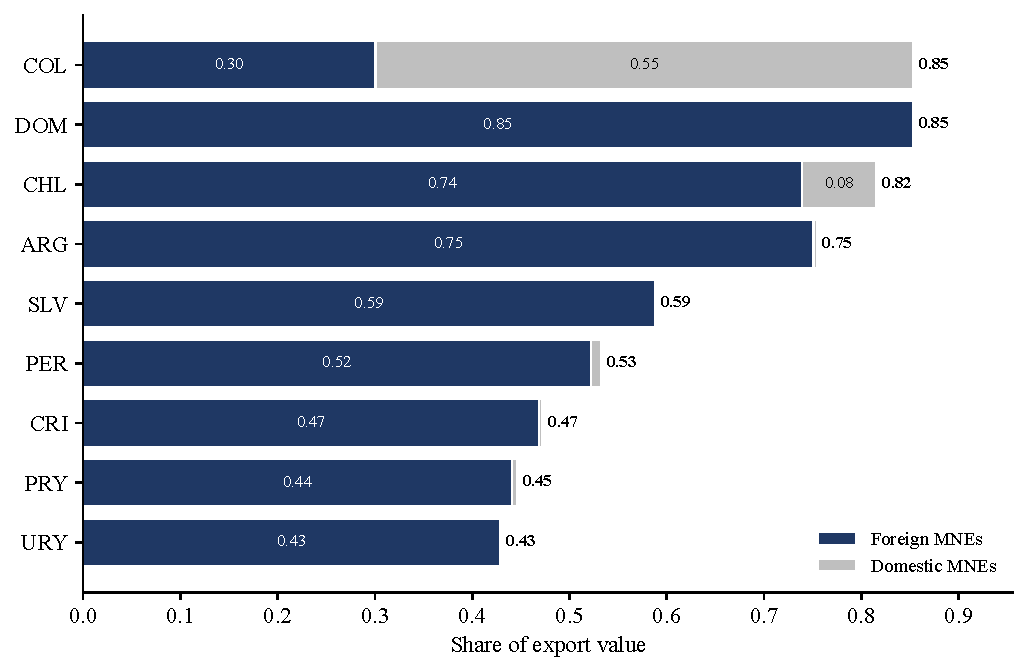
\includegraphics[width=0.8\textwidth,height=0.8\textheight,keepaspectratio]{figures/mining/fig_wp0_fig1_origin.pdf}%
  \caption{Mining and Fuels: Multinational Share of Export Value, by Exporting Country}%
  \label{fig:f1_mining}%
  \par\vspace{2pt}%
  \parbox{0.92\textwidth}{\footnotesize %
  \textit{Notes:} Shares of mining and fuels export value (HS 25--27 and 71), all available years pooled. The figure at the end of each bar is the total MNE share.\\[3pt]%
  \textit{Source:} Authors' calculations based on customs data matched to Orbis and Dun \& Bradstreet.}%
  \end{figure}
% ---- Table: Mining and Fuels: Multinational Share of Export Value, by Exporting Country
\begin{table}[H]\centering\small%
  \caption{Mining and Fuels: Multinational Share of Export Value, by Exporting Country}%
  \label{tab:f1n_mining}%
  \adjustbox{max width=\textwidth, max totalheight=0.8\textheight}{\begin{tabular}{lrrrr}
\toprule
Origin & Foreign & Domestic & All MNEs & Value (US\$bn/yr) \\
\midrule
COL & 0.301 & 0.553 & 0.853 & 27.9 \\
DOM & 0.853 & 0.000 & 0.853 & 2.0 \\
CHL & 0.739 & 0.076 & 0.815 & 10.2 \\
ARG & 0.751 & 0.003 & 0.754 & 6.6 \\
SLV & 0.588 & 0.000 & 0.588 & 0.2 \\
PER & 0.522 & 0.010 & 0.532 & 25.3 \\
CRI & 0.469 & 0.003 & 0.472 & 0.1 \\
PRY & 0.441 & 0.005 & 0.446 & 0.1 \\
URY & 0.429 & 0.000 & 0.429 & 0.2 \\
\midrule
All & 0.492 & 0.245 & 0.737 & 72.4 \\
\bottomrule
\end{tabular}
}%
  \par\vspace{3pt}%
  \begin{minipage}{0.95\textwidth}\footnotesize %
  \textit{Notes:} Shares of mining and fuels export value (HS 25--27 and 71), all available years pooled. Values are annual averages in US\$ billion.\\[3pt]%
  \textit{Source:} Authors' calculations based on customs data matched to Orbis and Dun \& Bradstreet.%
  \end{minipage}%
  \end{table}

\subsection{By Parent Country}
% ---- Figure: Mining and Fuels: Multinational Share of Export Value, by Exporting Country and Parent Country
\begin{figure}[H]\centering%
  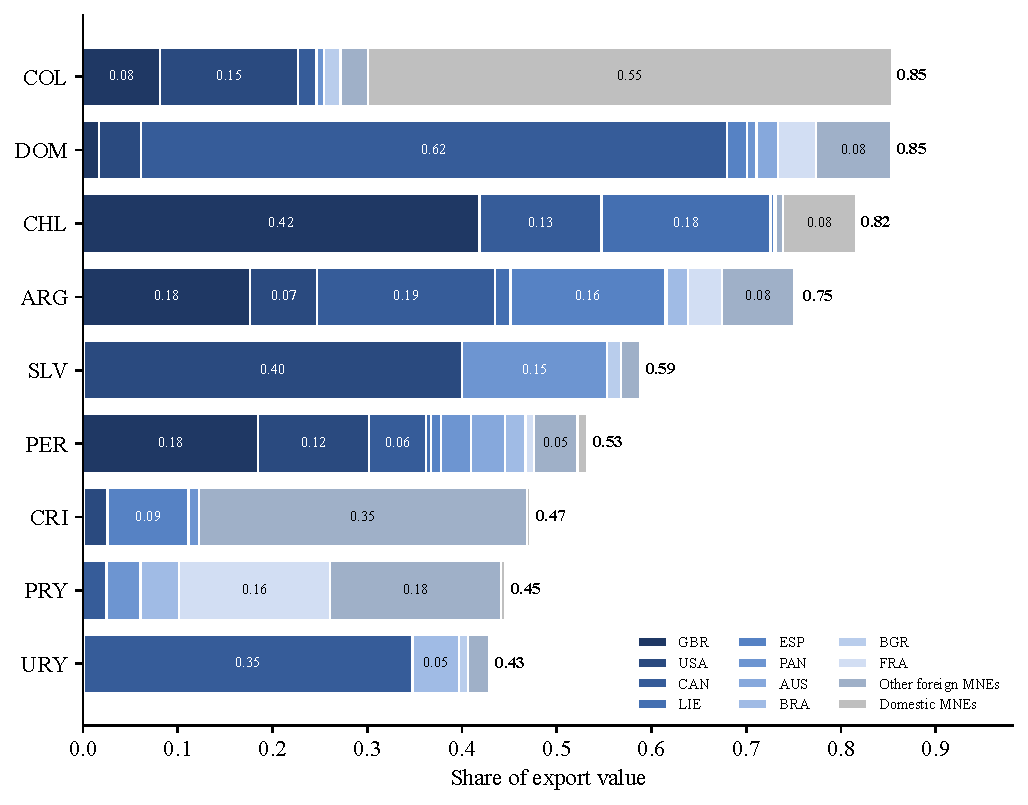
\includegraphics[width=0.92\textwidth,height=0.8\textheight,keepaspectratio]{figures/mining/fig_wp1a_origin_by_parent.pdf}%
  \caption{Mining and Fuels: Multinational Share of Export Value, by Exporting Country and Parent Country}%
  \label{fig:f1p_mining}%
  \par\vspace{2pt}%
  \parbox{0.92\textwidth}{\footnotesize %
  \textit{Notes:} Shares of mining and fuels export value (HS 25--27 and 71), all available years pooled. Foreign MNEs split by country of the ultimate parent; the ten largest parent countries are shown separately.\\[3pt]%
  \textit{Source:} Authors' calculations based on customs data matched to Orbis and Dun \& Bradstreet.}%
  \end{figure}
% ---- Table: Mining and Fuels: Multinational Share of Export Value, by Exporting Country and Parent Country
\begin{table}[H]\centering\small%
  \caption{Mining and Fuels: Multinational Share of Export Value, by Exporting Country and Parent Country}%
  \label{tab:f1pn_mining}%
  \adjustbox{max width=\textwidth, max totalheight=0.8\textheight}{\begin{tabular}{lcccccccccccccc}
\toprule
Origin & GBR & USA & CAN & LIE & ESP & PAN & AUS & BRA & BGR & FRA & Other & Domestic & All MNEs & Value (US\$bn/yr) \\
\midrule
COL & 0.081 & 0.146 & 0.019 & 0.000 & 0.001 & 0.008 & 0.000 & 0.000 & 0.017 & 0.001 & 0.028 & 0.553 & 0.853 & 27.9 \\
DOM & 0.017 & 0.044 & 0.619 & 0.000 & 0.021 & 0.010 & 0.022 & 0.000 & 0.000 & 0.041 & 0.079 & 0.000 & 0.853 & 2.0 \\
CHL & 0.418 & 0.001 & 0.129 & 0.178 & 0.003 & 0.000 & 0.003 & 0.000 & 0.000 & 0.000 & 0.007 & 0.076 & 0.815 & 10.2 \\
ARG & 0.176 & 0.071 & 0.188 & 0.016 & 0.163 & 0.001 & 0.001 & 0.022 & 0.000 & 0.036 & 0.076 & 0.003 & 0.754 & 6.6 \\
SLV & 0.001 & 0.399 & 0.000 & 0.000 & 0.000 & 0.153 & 0.000 & 0.000 & 0.015 & 0.000 & 0.020 & 0.000 & 0.588 & 0.2 \\
PER & 0.185 & 0.117 & 0.060 & 0.006 & 0.010 & 0.032 & 0.036 & 0.021 & 0.001 & 0.008 & 0.046 & 0.010 & 0.532 & 25.3 \\
CRI & 0.000 & 0.026 & 0.000 & 0.000 & 0.085 & 0.011 & 0.000 & 0.000 & 0.000 & 0.000 & 0.347 & 0.003 & 0.472 & 0.1 \\
PRY & 0.000 & 0.000 & 0.025 & 0.000 & 0.000 & 0.036 & 0.000 & 0.041 & 0.000 & 0.159 & 0.181 & 0.005 & 0.446 & 0.1 \\
URY & 0.000 & 0.000 & 0.347 & 0.000 & 0.001 & 0.000 & 0.000 & 0.049 & 0.010 & 0.000 & 0.022 & 0.000 & 0.429 & 0.2 \\
\bottomrule
\end{tabular}
}%
  \par\vspace{3pt}%
  \begin{minipage}{0.95\textwidth}\footnotesize %
  \textit{Notes:} Shares of mining and fuels export value (HS 25--27 and 71), all available years pooled. Other: all remaining foreign parents. Values are annual averages in US\$ billion.\\[3pt]%
  \textit{Source:} Authors' calculations based on customs data matched to Orbis and Dun \& Bradstreet.%
  \end{minipage}%
  \end{table}
% ---- Figure: Mining and Fuels: Export Value by Exporting Country and Parent Country
\begin{figure}[H]\centering%
  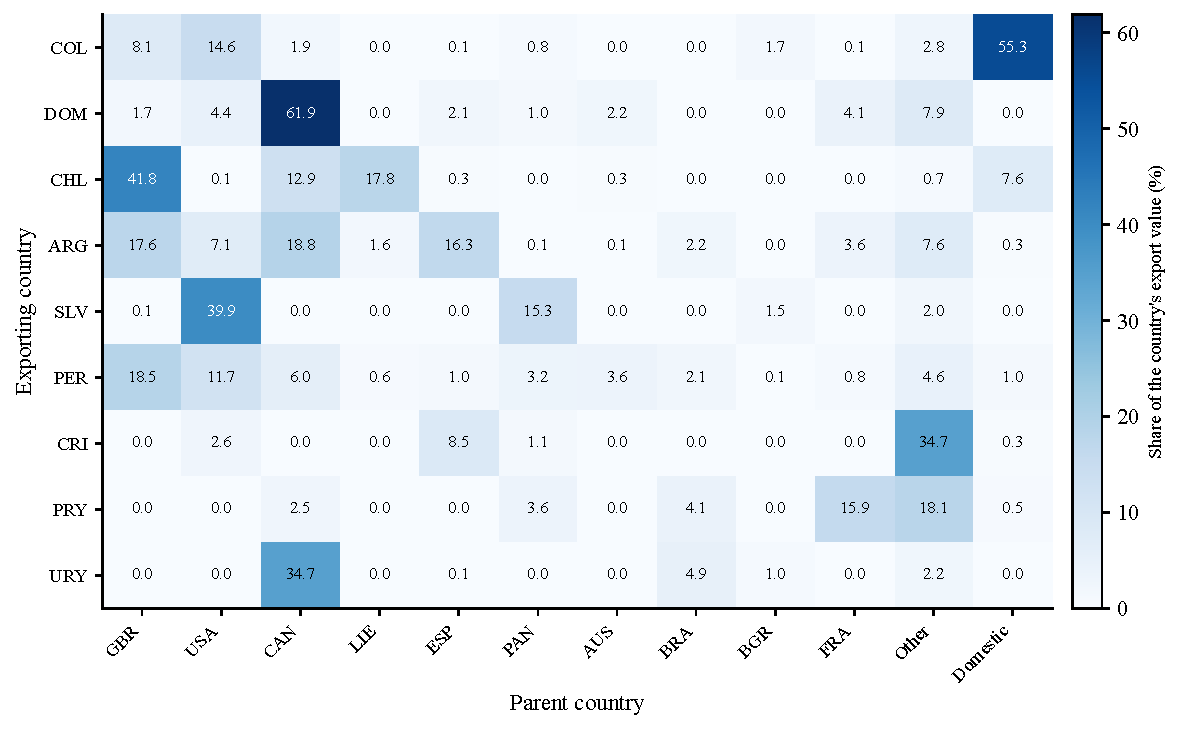
\includegraphics[width=0.9\textwidth,height=0.8\textheight,keepaspectratio]{figures/mining/fig_wp1a_origin_x_parent_heatmap.pdf}%
  \caption{Mining and Fuels: Export Value by Exporting Country and Parent Country}%
  \label{fig:f1hm_mining}%
  \par\vspace{2pt}%
  \parbox{0.92\textwidth}{\footnotesize %
  \textit{Notes:} Percent of each country's mining and fuels export value, by country of the ultimate parent of the exporter.\\[3pt]%
  \textit{Source:} Authors' calculations based on customs data matched to Orbis and Dun \& Bradstreet.}%
  \end{figure}

\section{Fact 2: Foreign Multinationals Specialize in Complex Products, Domestic Multinationals in Primary Goods}\label{sec:f2_mining}

\subsection{Product Complexity and Technology}
% ---- Figure: Mining and Fuels: Multinational Share of Export Value, by Product Complexity Quintile
\begin{figure}[H]\centering%
  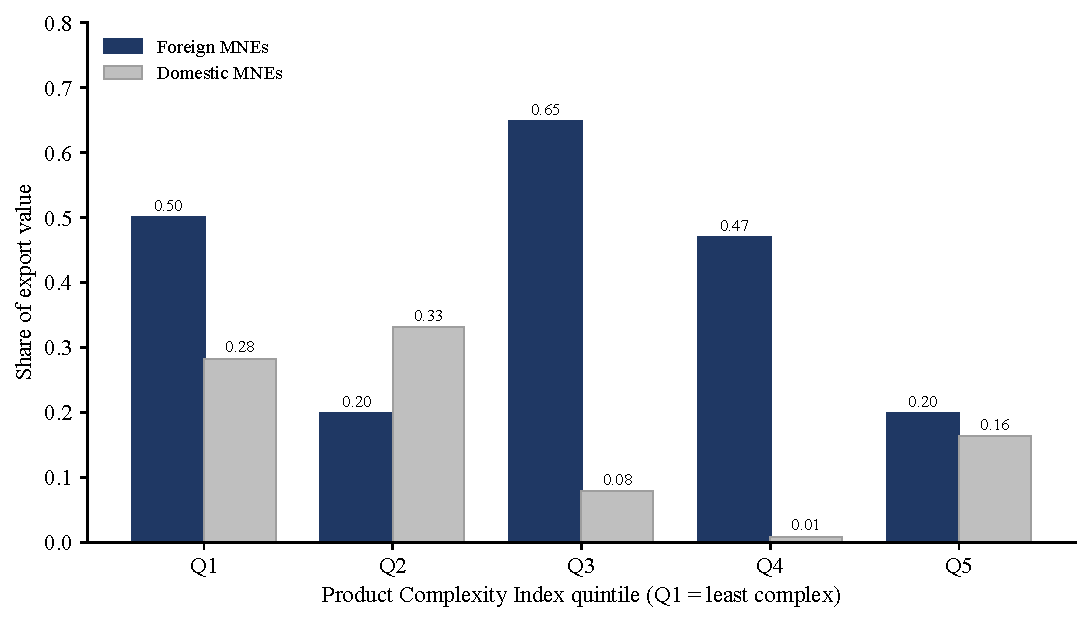
\includegraphics[width=0.78\textwidth,height=0.8\textheight,keepaspectratio]{figures/mining/fig_wp0_fig2_pci.pdf}%
  \caption{Mining and Fuels: Multinational Share of Export Value, by Product Complexity Quintile}%
  \label{fig:pci_mining}%
  \par\vspace{2pt}%
  \parbox{0.92\textwidth}{\footnotesize %
  \textit{Notes:} Shares of mining and fuels export value (HS 25--27 and 71), all available years pooled. Quintiles of the Hausmann--Hidalgo Product Complexity Index across HS6 products (Q1 = least complex).\\[3pt]%
  \textit{Source:} Authors' calculations based on customs data matched to Orbis and Dun \& Bradstreet.}%
  \end{figure}
% ---- Figure: Mining and Fuels: Multinational Share of Export Value, by Technology Class
\begin{figure}[H]\centering%
  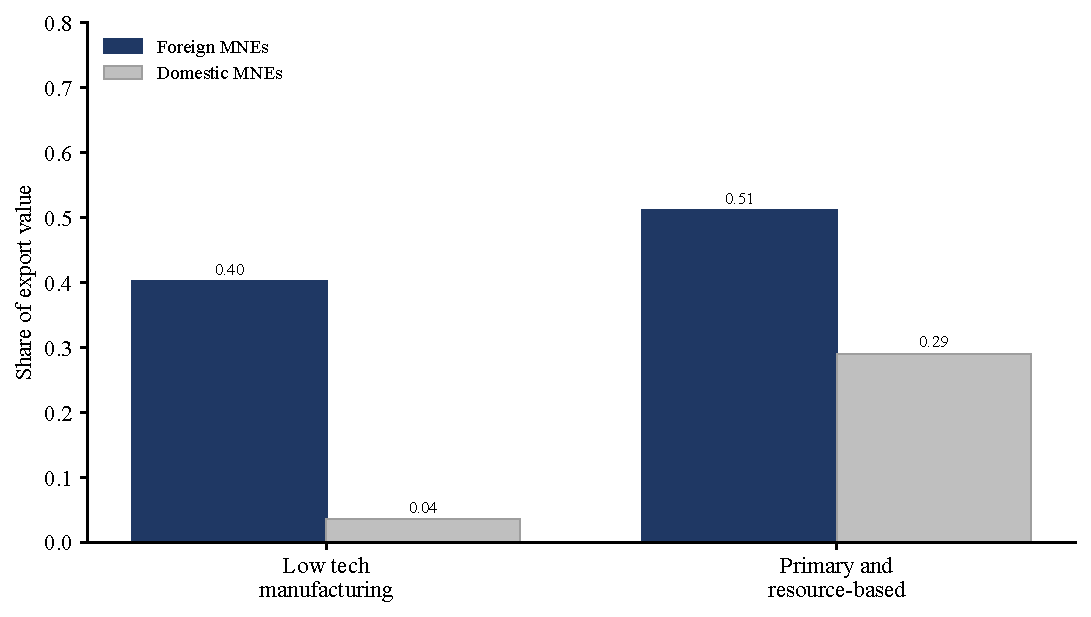
\includegraphics[width=0.78\textwidth,height=0.8\textheight,keepaspectratio]{figures/mining/fig_wp0_fig3_lall.pdf}%
  \caption{Mining and Fuels: Multinational Share of Export Value, by Technology Class}%
  \label{fig:lall_mining}%
  \par\vspace{2pt}%
  \parbox{0.92\textwidth}{\footnotesize %
  \textit{Notes:} Shares of mining and fuels export value (HS 25--27 and 71), all available years pooled. Lall (2000) technology classes: primary and resource-based products, and low-, medium- and high-technology manufactures.\\[3pt]%
  \textit{Source:} Authors' calculations based on customs data matched to Orbis and Dun \& Bradstreet.}%
  \end{figure}

\subsection{By Parent Country}
% ---- Figure: Mining and Fuels: Multinational Share of Export Value, by Product Complexity Quintile and Parent Country
\begin{figure}[H]\centering%
  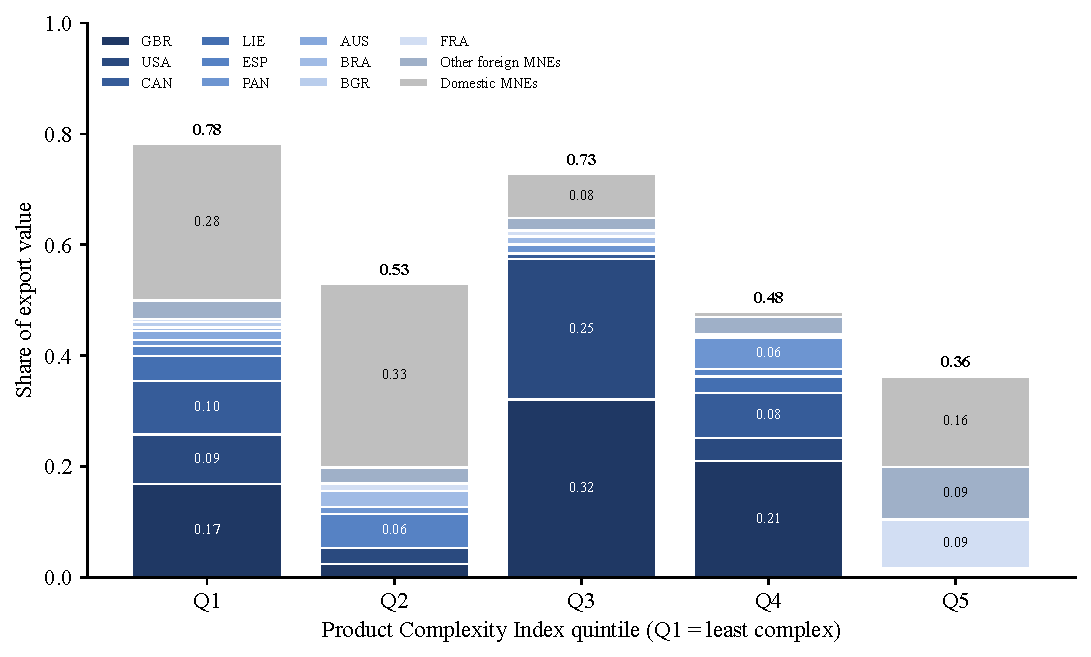
\includegraphics[width=0.92\textwidth,height=0.8\textheight,keepaspectratio]{figures/mining/fig_wp1a_pci_by_parent.pdf}%
  \caption{Mining and Fuels: Multinational Share of Export Value, by Product Complexity Quintile and Parent Country}%
  \label{fig:pci_p_mining}%
  \par\vspace{2pt}%
  \parbox{0.92\textwidth}{\footnotesize %
  \textit{Notes:} Shares of mining and fuels export value (HS 25--27 and 71), all available years pooled. Foreign MNEs split by country of the ultimate parent. Quintiles of the Hausmann--Hidalgo Product Complexity Index across HS6 products (Q1 = least complex).\\[3pt]%
  \textit{Source:} Authors' calculations based on customs data matched to Orbis and Dun \& Bradstreet.}%
  \end{figure}
% ---- Table: Mining and Fuels: Multinational Share of Export Value, by Product Complexity Quintile and Parent Country
\begin{table}[H]\centering\small%
  \caption{Mining and Fuels: Multinational Share of Export Value, by Product Complexity Quintile and Parent Country}%
  \label{tab:pci_pn_mining}%
  \adjustbox{max width=\textwidth, max totalheight=0.8\textheight}{\begin{tabular}{lcccccccccccccc}
\toprule
PCI quintile & GBR & USA & CAN & LIE & ESP & PAN & AUS & BRA & BGR & FRA & Other & Domestic & All MNEs & Value (US\$bn/yr) \\
\midrule
Q1 & 0.168 & 0.089 & 0.097 & 0.045 & 0.017 & 0.011 & 0.016 & 0.006 & 0.010 & 0.006 & 0.033 & 0.282 & 0.782 & 52.4 \\
Q2 & 0.024 & 0.028 & 0.000 & 0.000 & 0.062 & 0.012 & 0.000 & 0.028 & 0.000 & 0.014 & 0.029 & 0.331 & 0.529 & 6.1 \\
Q3 & 0.321 & 0.254 & 0.008 & 0.001 & 0.001 & 0.016 & 0.000 & 0.014 & 0.001 & 0.010 & 0.023 & 0.079 & 0.727 & 9.0 \\
Q4 & 0.210 & 0.042 & 0.081 & 0.030 & 0.014 & 0.056 & 0.002 & 0.002 & 0.000 & 0.001 & 0.032 & 0.008 & 0.478 & 4.0 \\
Q5 & 0.001 & 0.004 & 0.004 & 0.003 & 0.001 & 0.002 & 0.001 & 0.000 & 0.000 & 0.087 & 0.094 & 0.164 & 0.362 & 0.1 \\
\bottomrule
\end{tabular}
}%
  \par\vspace{3pt}%
  \begin{minipage}{0.95\textwidth}\footnotesize %
  \textit{Notes:} Shares of mining and fuels export value (HS 25--27 and 71), all available years pooled. Other: all remaining foreign parents. Values are annual averages in US\$ billion.\\[3pt]%
  \textit{Source:} Authors' calculations based on customs data matched to Orbis and Dun \& Bradstreet.%
  \end{minipage}%
  \end{table}
% ---- Figure: Mining and Fuels: Multinational Share of Export Value, by Technology Class and Parent Country
\begin{figure}[H]\centering%
  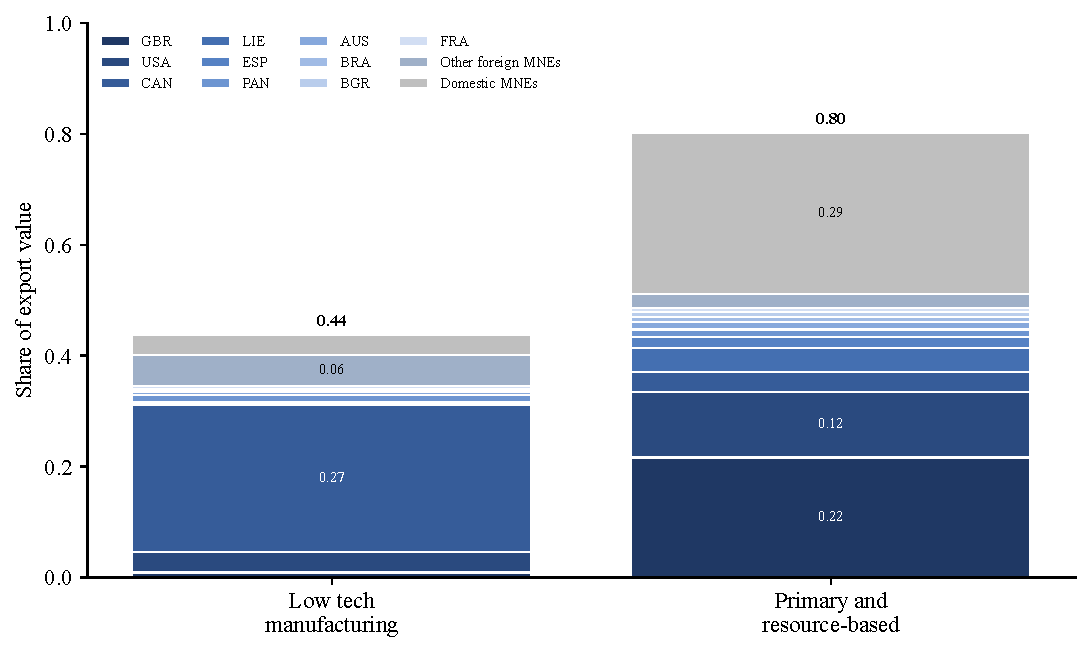
\includegraphics[width=0.92\textwidth,height=0.8\textheight,keepaspectratio]{figures/mining/fig_wp1a_lall_by_parent.pdf}%
  \caption{Mining and Fuels: Multinational Share of Export Value, by Technology Class and Parent Country}%
  \label{fig:lall_p_mining}%
  \par\vspace{2pt}%
  \parbox{0.92\textwidth}{\footnotesize %
  \textit{Notes:} Shares of mining and fuels export value (HS 25--27 and 71), all available years pooled. Foreign MNEs split by country of the ultimate parent. Lall (2000) technology classes: primary and resource-based products, and low-, medium- and high-technology manufactures.\\[3pt]%
  \textit{Source:} Authors' calculations based on customs data matched to Orbis and Dun \& Bradstreet.}%
  \end{figure}
% ---- Table: Mining and Fuels: Multinational Share of Export Value, by Technology Class and Parent Country
\begin{table}[H]\centering\small%
  \caption{Mining and Fuels: Multinational Share of Export Value, by Technology Class and Parent Country}%
  \label{tab:lall_pn_mining}%
  \adjustbox{max width=\textwidth, max totalheight=0.8\textheight}{\begin{tabular}{lcccccccccccccc}
\toprule
Technology category & GBR & USA & CAN & LIE & ESP & PAN & AUS & BRA & BGR & FRA & Other & Domestic & All MNEs & Value (US\$bn/yr) \\
\midrule
Low tech manufacturing & 0.009 & 0.037 & 0.266 & 0.000 & 0.004 & 0.014 & 0.005 & 0.004 & 0.001 & 0.006 & 0.056 & 0.036 & 0.438 & 14.4 \\
Primary and resource-based & 0.217 & 0.118 & 0.036 & 0.042 & 0.020 & 0.014 & 0.014 & 0.009 & 0.009 & 0.007 & 0.026 & 0.291 & 0.802 & 57.3 \\
\bottomrule
\end{tabular}
}%
  \par\vspace{3pt}%
  \begin{minipage}{0.95\textwidth}\footnotesize %
  \textit{Notes:} Shares of mining and fuels export value (HS 25--27 and 71), all available years pooled. Other: all remaining foreign parents. Values are annual averages in US\$ billion.\\[3pt]%
  \textit{Source:} Authors' calculations based on customs data matched to Orbis and Dun \& Bradstreet.%
  \end{minipage}%
  \end{table}
% ---- Figure: Mining and Fuels: Multinational Share of Export Value, by Product Sophistication and Location of the Parent
\begin{figure}[H]\centering%
  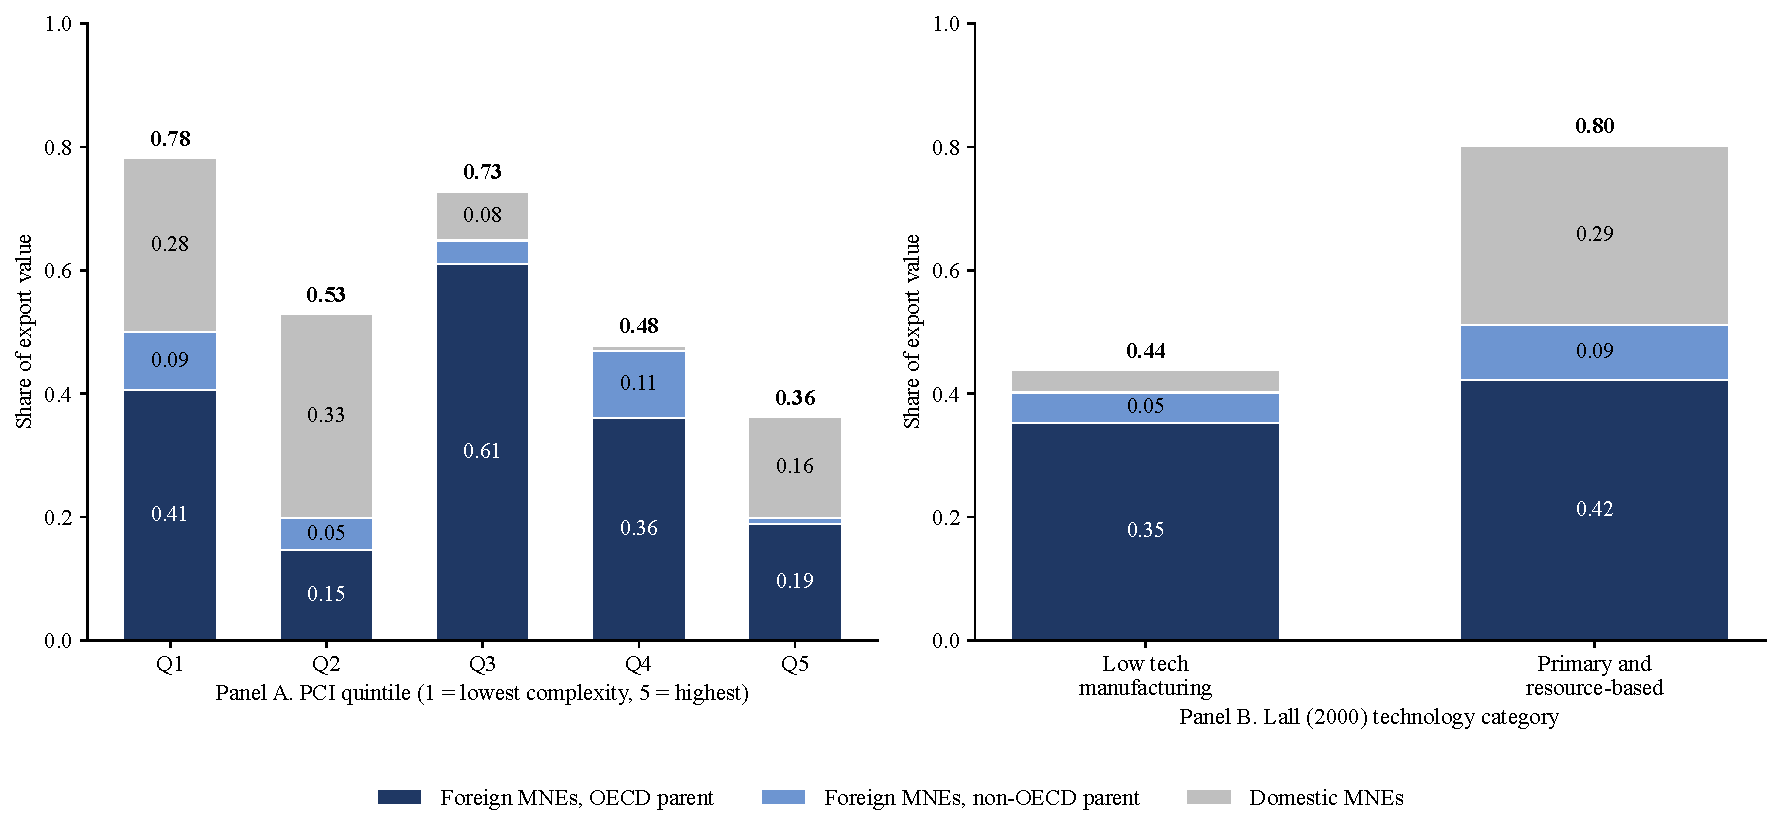
\includegraphics[width=1.0\textwidth,height=0.8\textheight,keepaspectratio]{figures/mining/fig_wp1a_pci_lall_by_oecd.pdf}%
  \caption{Mining and Fuels: Multinational Share of Export Value, by Product Sophistication and Location of the Parent}%
  \label{fig:oecd_mining}%
  \par\vspace{2pt}%
  \parbox{0.92\textwidth}{\footnotesize %
  \textit{Notes:} Shares of mining and fuels export value (HS 25--27 and 71), all available years pooled. Foreign MNEs are split by whether the ultimate parent is in an OECD member country. Panel A: Quintiles of the Hausmann--Hidalgo Product Complexity Index across HS6 products (Q1 = least complex). Panel B: Lall (2000) technology classes: primary and resource-based products, and low-, medium- and high-technology manufactures.\\[3pt]%
  \textit{Source:} Authors' calculations based on customs data matched to Orbis and Dun \& Bradstreet.}%
  \end{figure}

\subsection{Other Measures of Product Sophistication}
% ---- Figure: Mining and Fuels: Multinational Share of Export Value, by Quintile of Six Sophistication Measures
\begin{figure}[H]\centering%
  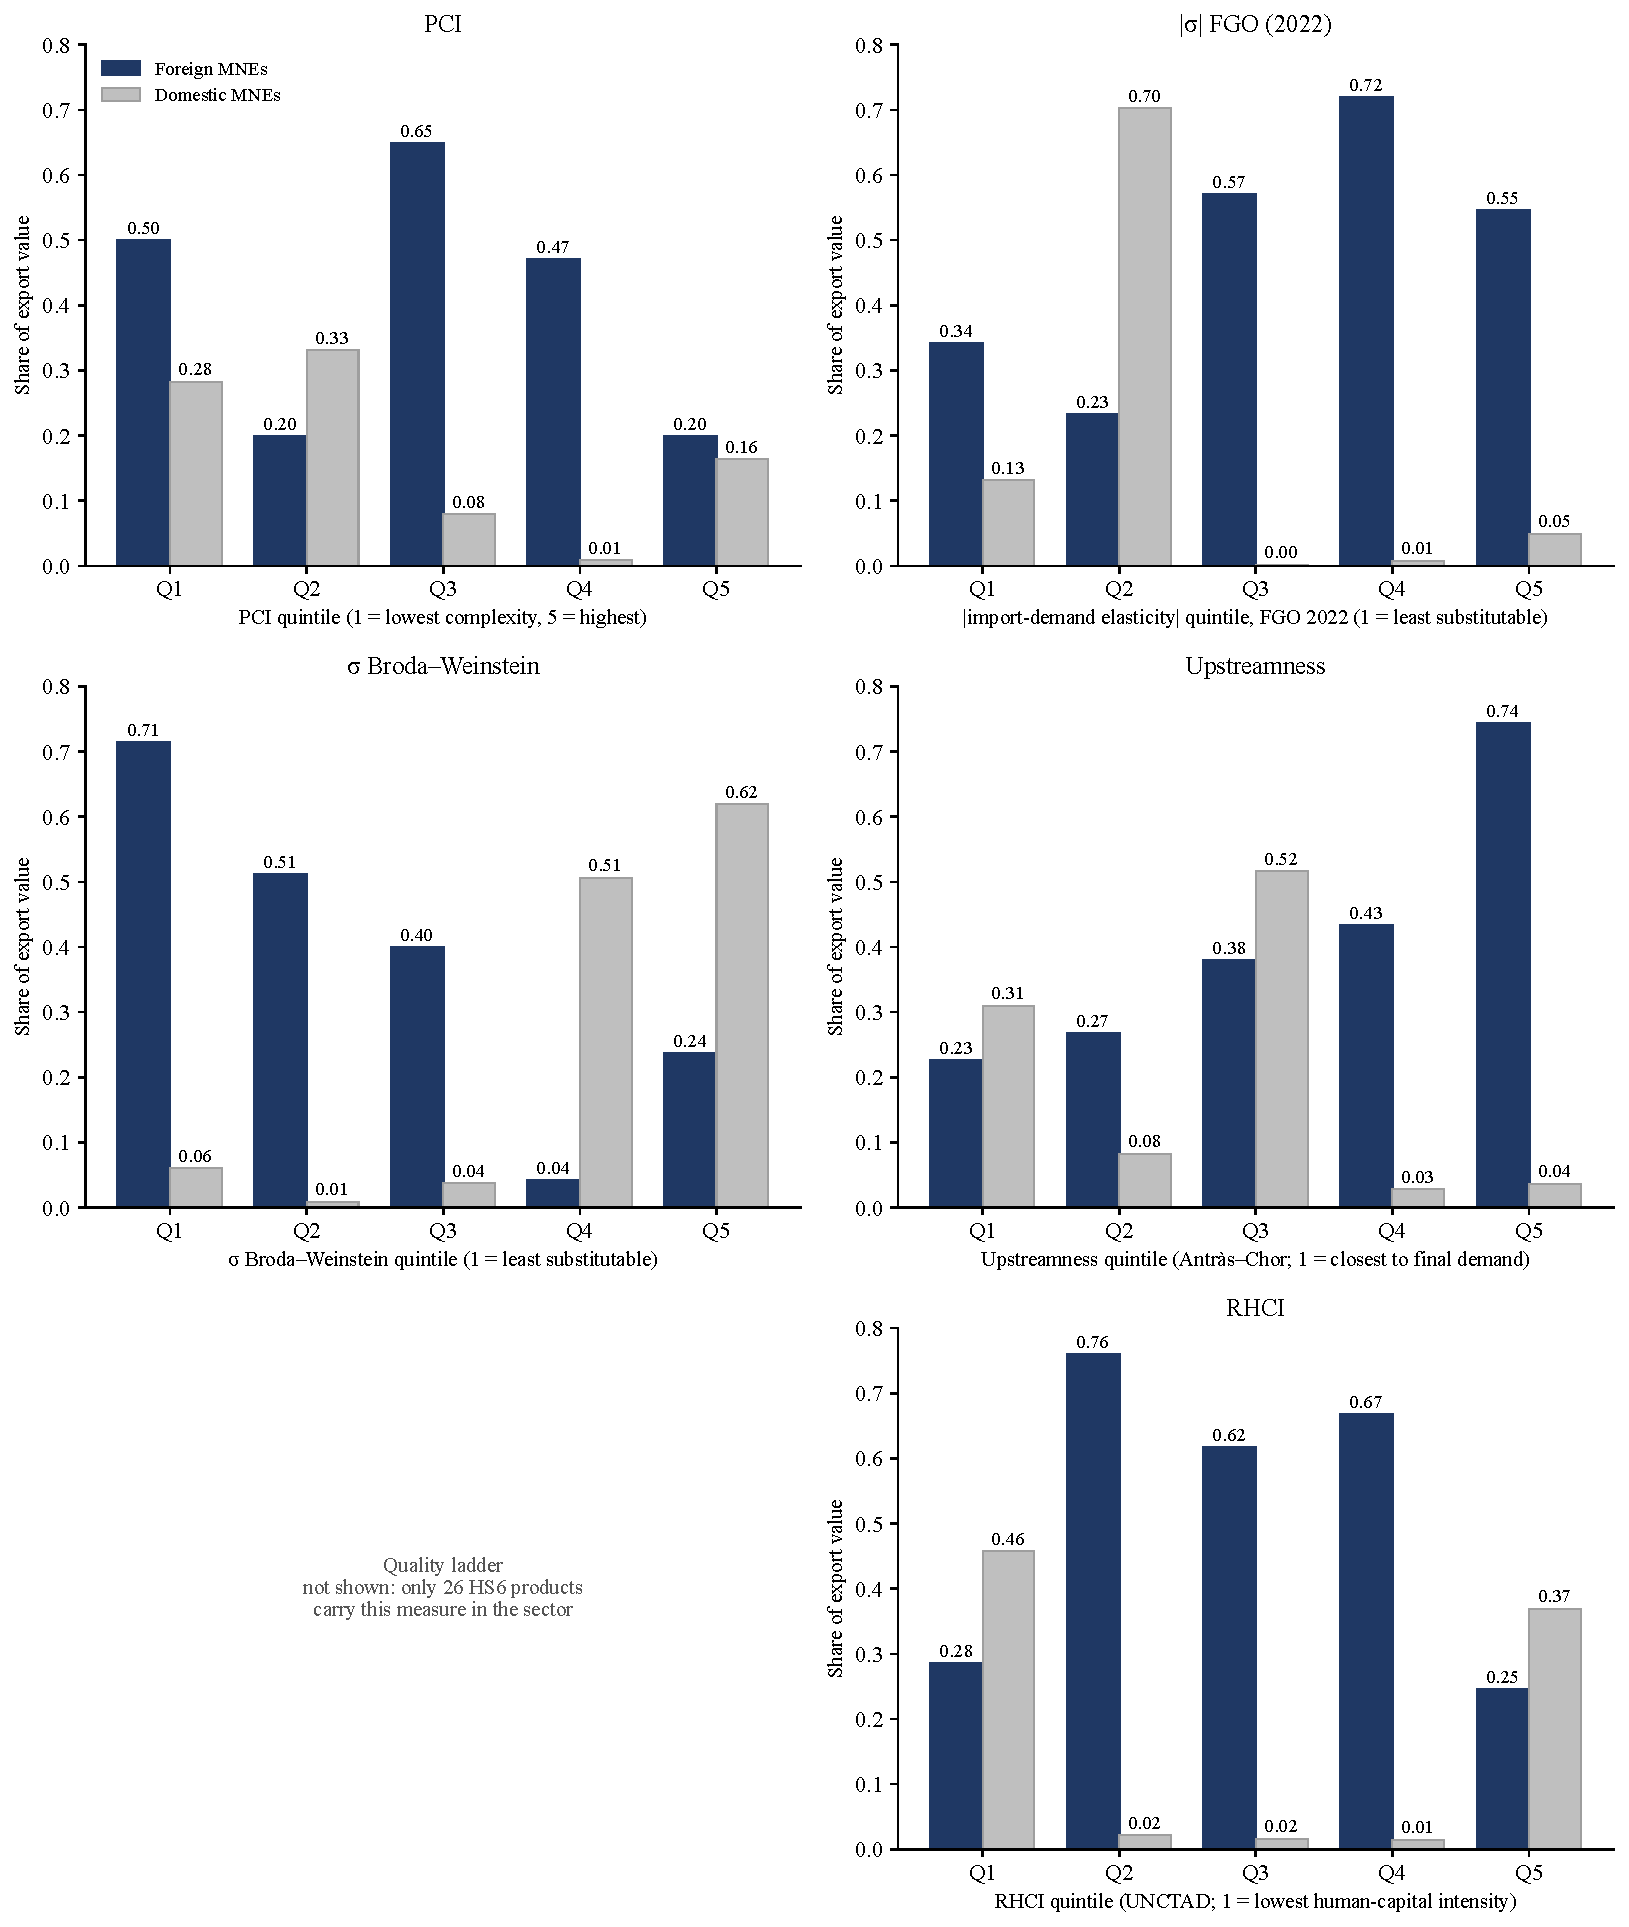
\includegraphics[width=1.0\textwidth,height=0.8\textheight,keepaspectratio]{figures/mining/fig_wp1b_panel_quintiles.pdf}%
  \caption{Mining and Fuels: Multinational Share of Export Value, by Quintile of Six Sophistication Measures}%
  \label{fig:six_q_mining}%
  \par\vspace{2pt}%
  \parbox{0.92\textwidth}{\footnotesize %
  \textit{Notes:} Shares of mining and fuels export value (HS 25--27 and 71), all available years pooled. Quintiles computed over HS6 products. The six measures are the Product Complexity Index, the absolute import-demand elasticity of Fontagn\'e, Guimbard and Orefice (2022), the elasticity of substitution of Broda and Weinstein, upstreamness, the quality ladder and the revealed human-capital intensity of UNCTAD.\\[3pt]%
  \textit{Source:} Authors' calculations based on customs data matched to Orbis and Dun \& Bradstreet.}%
  \end{figure}
% ---- Figure: Mining and Fuels: Multinational Share of Export Value, by Quintile of the Import-Demand Elasticity
\begin{figure}[H]\centering%
  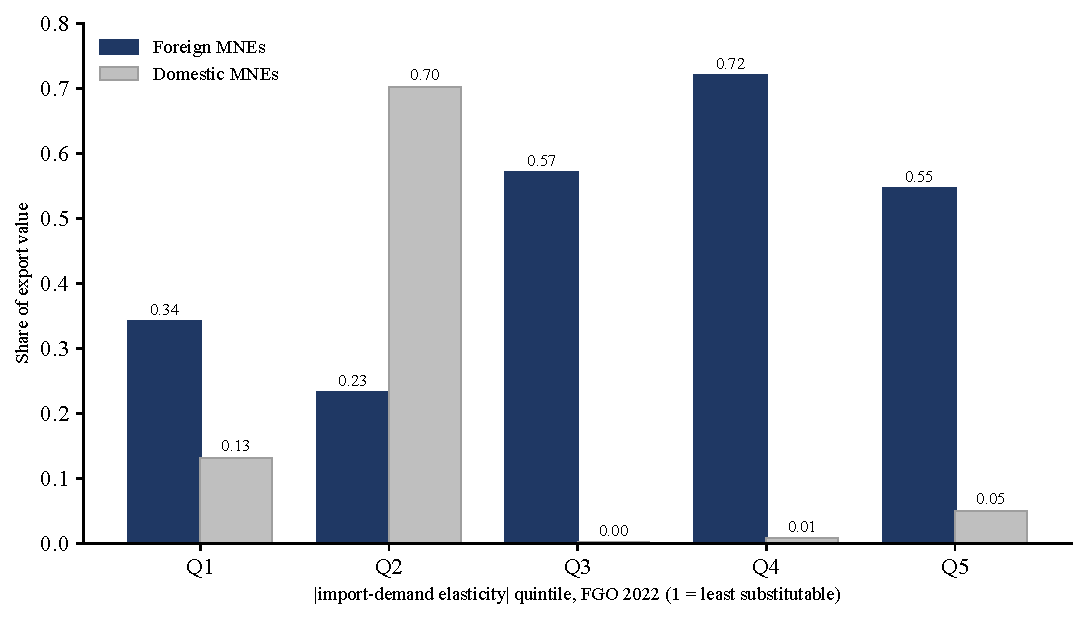
\includegraphics[width=0.78\textwidth,height=0.8\textheight,keepaspectratio]{figures/mining/fig_wp1b_sigma_fgo_abs_quintile.pdf}%
  \caption{Mining and Fuels: Multinational Share of Export Value, by Quintile of the Import-Demand Elasticity}%
  \label{fig:fgo_q_mining}%
  \par\vspace{2pt}%
  \parbox{0.92\textwidth}{\footnotesize %
  \textit{Notes:} Shares of mining and fuels export value (HS 25--27 and 71), all available years pooled. Quintiles of the absolute import-demand elasticity of Fontagn\'e, Guimbard and Orefice (2022) across HS6 products; higher quintiles are more substitutable products.\\[3pt]%
  \textit{Source:} Authors' calculations based on customs data matched to Orbis and Dun \& Bradstreet.}%
  \end{figure}
% ---- Figure: Mining and Fuels: Distribution of Export Value across Six Sophistication Measures
\begin{figure}[H]\centering%
  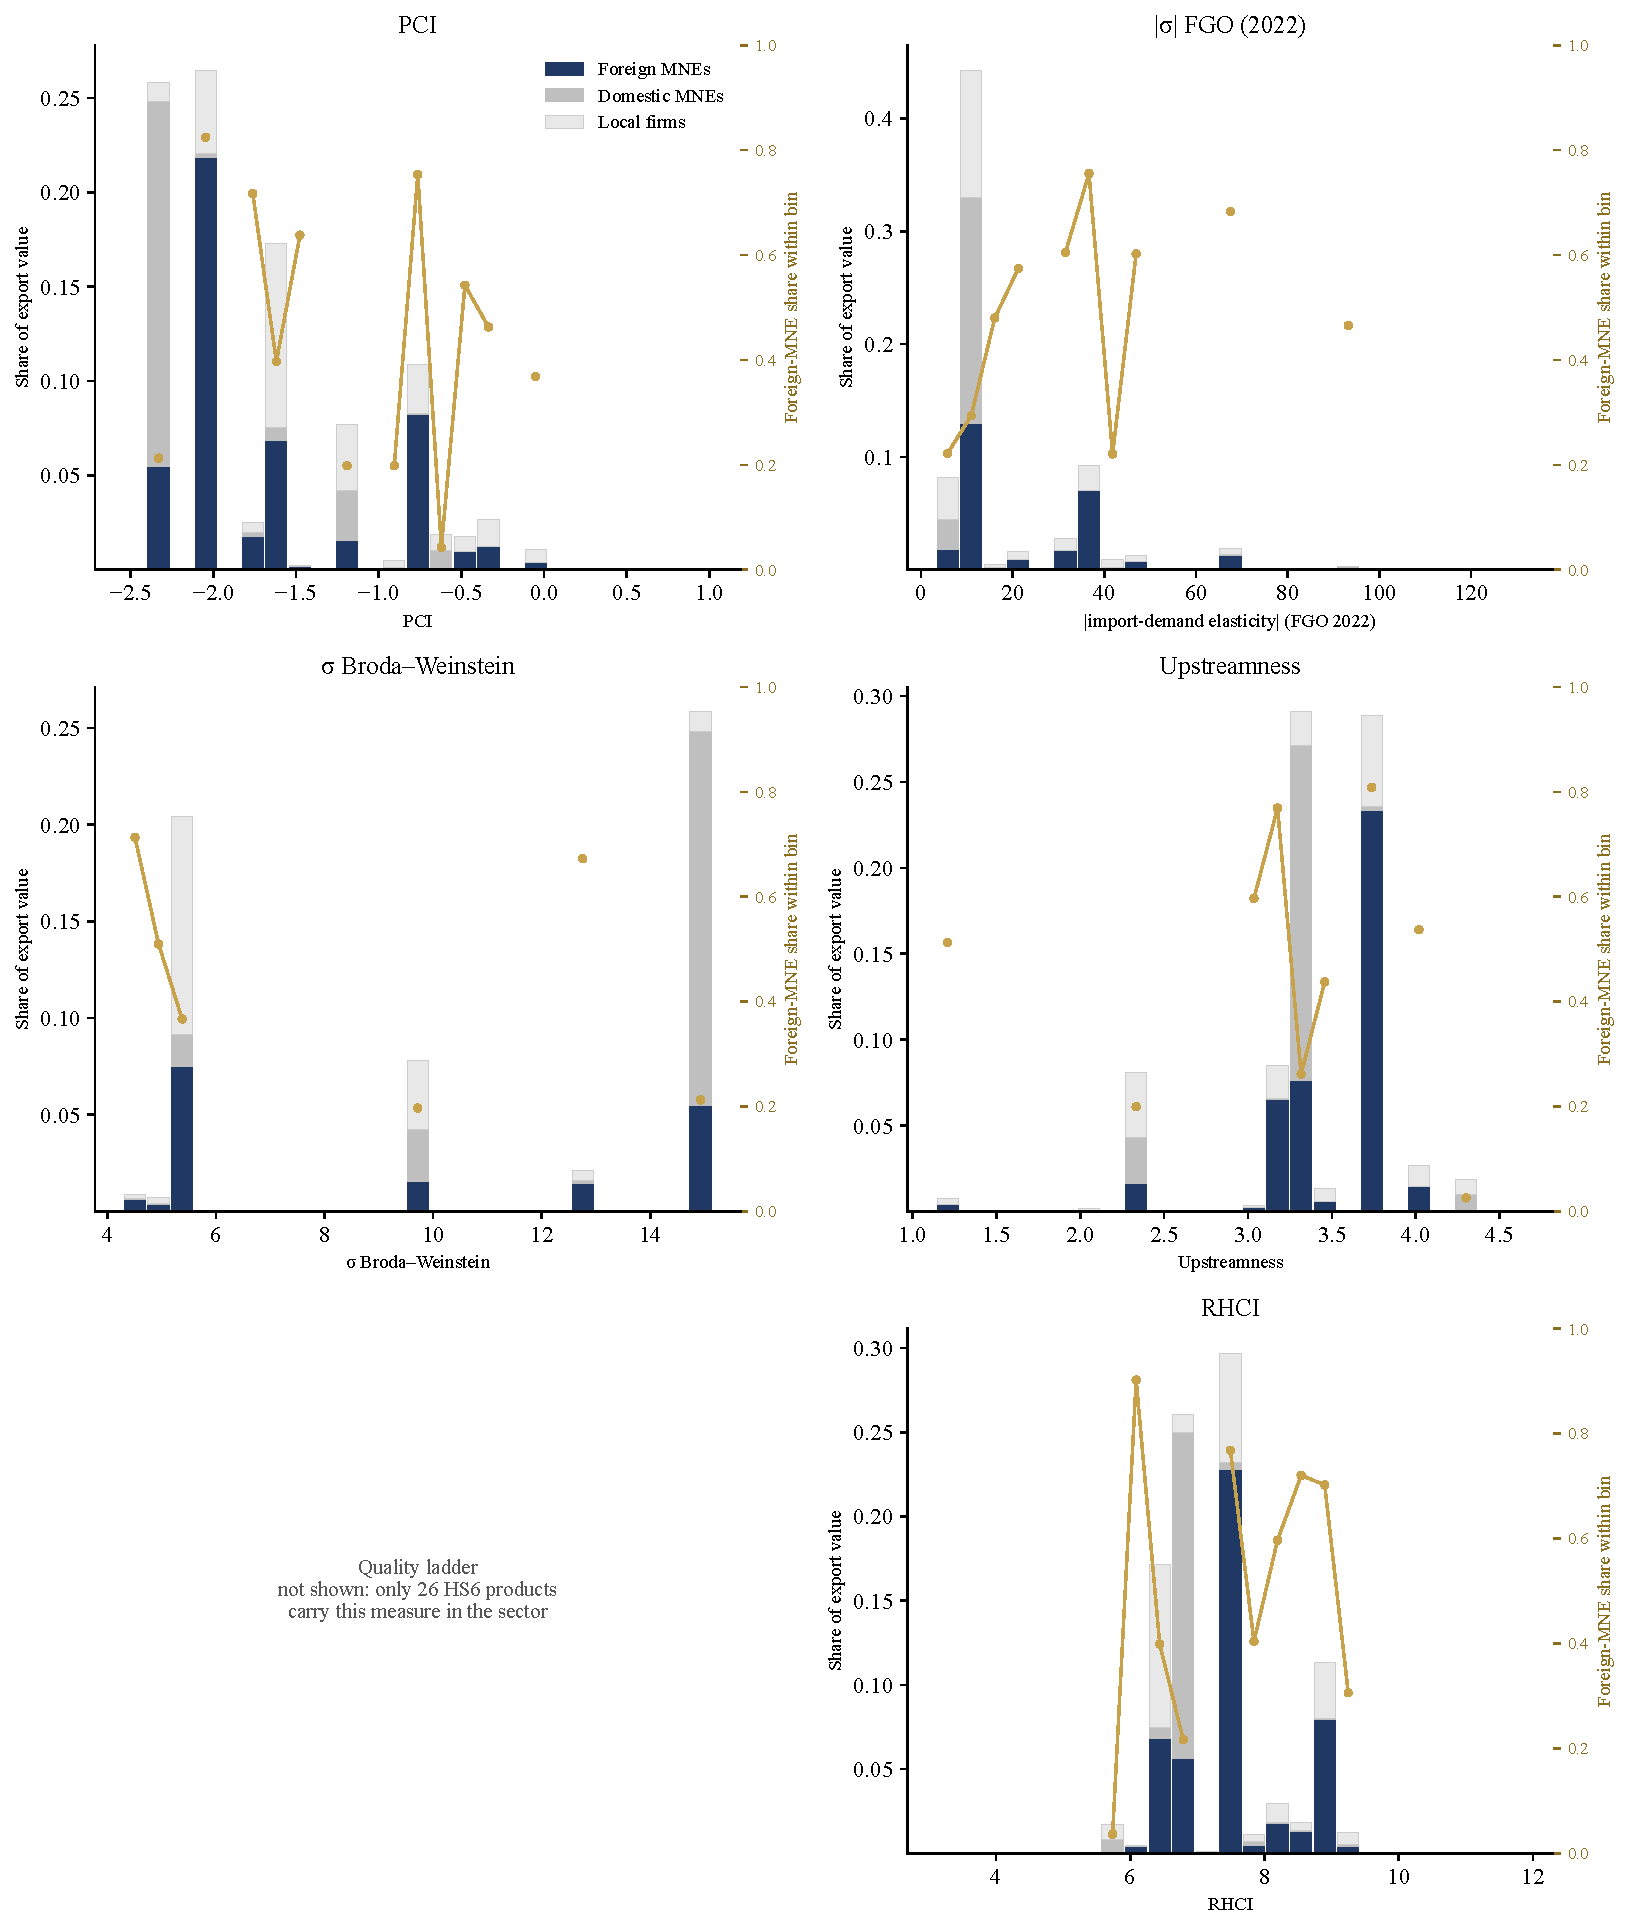
\includegraphics[width=1.0\textwidth,height=0.8\textheight,keepaspectratio]{figures/mining/fig_wp1b_panel_hist.pdf}%
  \caption{Mining and Fuels: Distribution of Export Value across Six Sophistication Measures}%
  \label{fig:six_h_mining}%
  \par\vspace{2pt}%
  \parbox{0.92\textwidth}{\footnotesize %
  \textit{Notes:} Bars: mining and fuels export value (HS 25--27 and 71) in each bin, by type of exporter. Line (right axis): foreign-MNE share of each bin. The six measures are the Product Complexity Index, the absolute import-demand elasticity of Fontagn\'e, Guimbard and Orefice (2022), the elasticity of substitution of Broda and Weinstein, upstreamness, the quality ladder and the revealed human-capital intensity of UNCTAD.\\[3pt]%
  \textit{Source:} Authors' calculations based on customs data matched to Orbis and Dun \& Bradstreet.}%
  \end{figure}
% ---- Figure: Mining and Fuels: Distribution of Export Value across the Import-Demand Elasticity
\begin{figure}[H]\centering%
  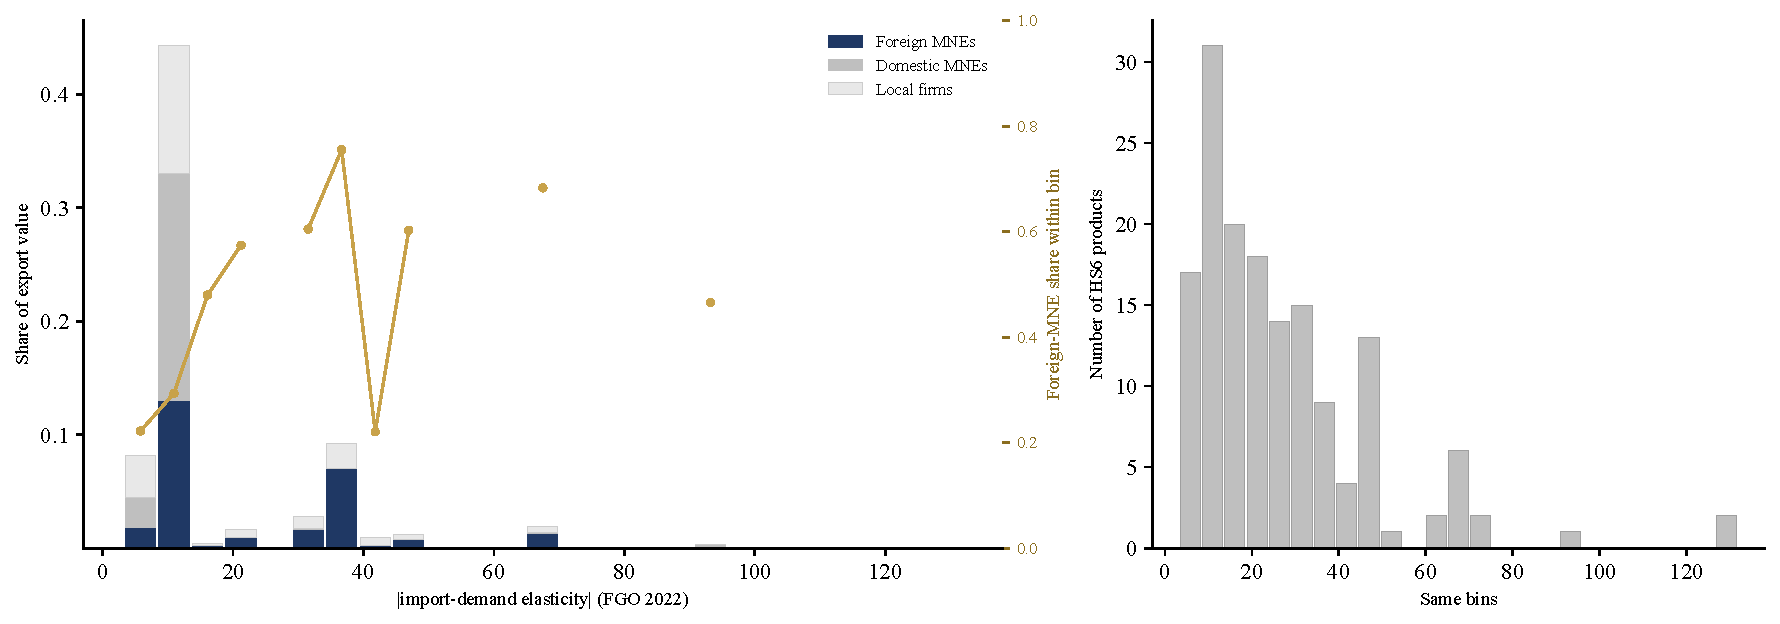
\includegraphics[width=1.0\textwidth,height=0.8\textheight,keepaspectratio]{figures/mining/fig_wp1b_hist_sigma_fgo_abs.pdf}%
  \caption{Mining and Fuels: Distribution of Export Value across the Import-Demand Elasticity}%
  \label{fig:fgo_h_mining}%
  \par\vspace{2pt}%
  \parbox{0.92\textwidth}{\footnotesize %
  \textit{Notes:} Left: export value in each bin, by type of exporter, and the foreign-MNE share of each bin. Right: number of HS6 products in each bin.\\[3pt]%
  \textit{Source:} Authors' calculations based on customs data matched to Orbis and Dun \& Bradstreet.}%
  \end{figure}
% ---- Figure: Mining and Fuels: Distribution of Export Value across the Product Complexity Index
\begin{figure}[H]\centering%
  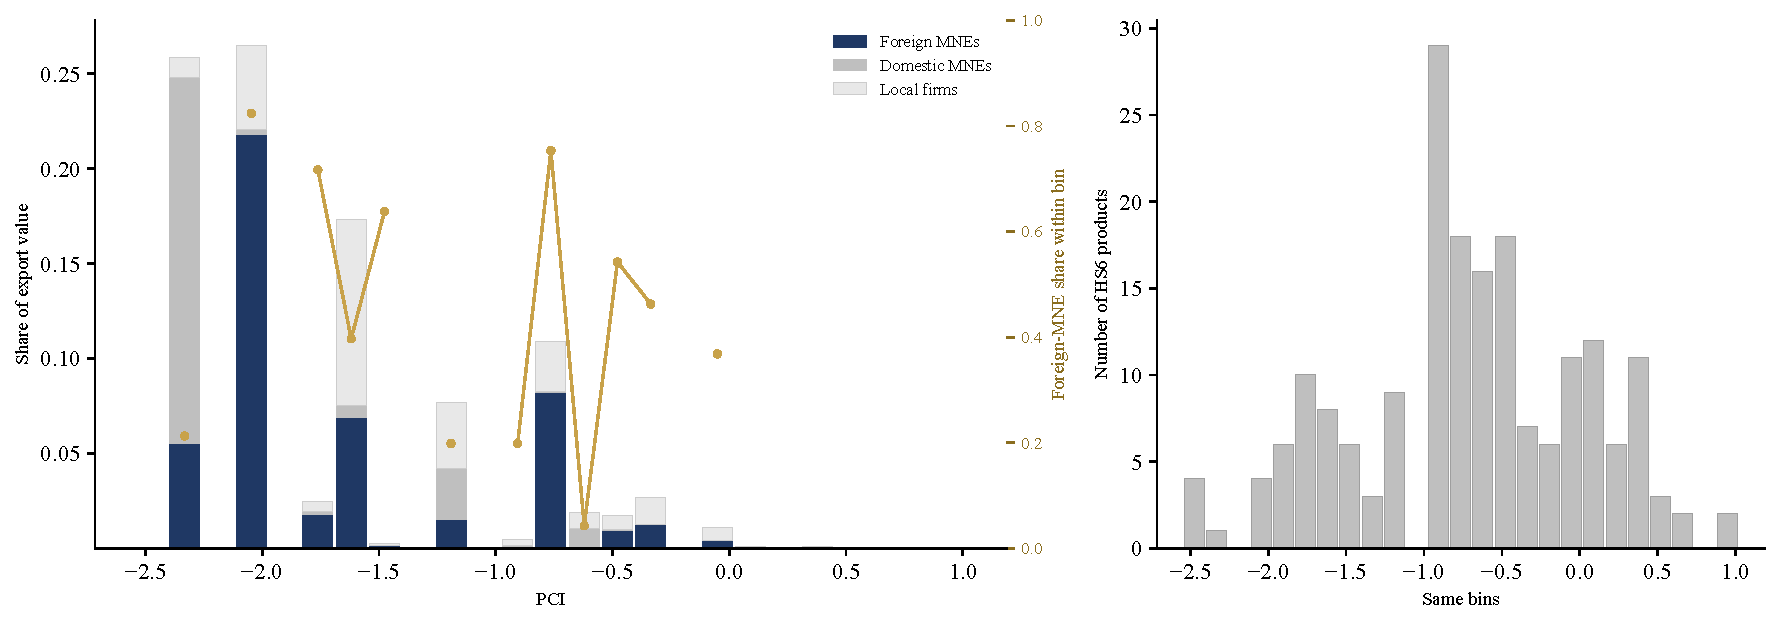
\includegraphics[width=1.0\textwidth,height=0.8\textheight,keepaspectratio]{figures/mining/fig_wp1b_hist_complexity.pdf}%
  \caption{Mining and Fuels: Distribution of Export Value across the Product Complexity Index}%
  \label{fig:pci_h_mining}%
  \par\vspace{2pt}%
  \parbox{0.92\textwidth}{\footnotesize %
  \textit{Notes:} Left: export value in each bin, by type of exporter, and the foreign-MNE share of each bin. Right: number of HS6 products in each bin.\\[3pt]%
  \textit{Source:} Authors' calculations based on customs data matched to Orbis and Dun \& Bradstreet.}%
  \end{figure}
% ---- Table: Mining and Fuels: Multinational Share of Export Value, by Quintile of Six Sophistication Measures
\begin{table}[H]\centering\small%
  \caption{Mining and Fuels: Multinational Share of Export Value, by Quintile of Six Sophistication Measures}%
  \label{tab:six_t_mining}%
  \adjustbox{max width=\textwidth, max totalheight=0.8\textheight}{\begin{tabular}{lccccc|ccccc}
\toprule
 & \multicolumn{5}{c}{Foreign MNE share} & \multicolumn{5}{c}{Domestic MNE share} \\
Measure & Q1 & Q2 & Q3 & Q4 & Q5 & Q1 & Q2 & Q3 & Q4 & Q5 \\
\midrule
PCI & 0.50 & 0.20 & 0.65 & 0.47 & 0.20 & 0.28 & 0.33 & 0.08 & 0.01 & 0.16 \\
$|\sigma|$ FGO (2022) & 0.34 & 0.23 & 0.57 & 0.72 & 0.55 & 0.13 & 0.70 & 0.00 & 0.01 & 0.05 \\
$\sigma$ Broda--Weinstein & 0.71 & 0.51 & 0.40 & 0.04 & 0.24 & 0.06 & 0.01 & 0.04 & 0.51 & 0.62 \\
Upstreamness & 0.23 & 0.27 & 0.38 & 0.43 & 0.74 & 0.31 & 0.08 & 0.52 & 0.03 & 0.04 \\
Quality ladder & -- & -- & -- & -- & -- & -- & -- & -- & -- & -- \\
RHCI & 0.28 & 0.76 & 0.62 & 0.67 & 0.25 & 0.46 & 0.02 & 0.02 & 0.01 & 0.37 \\
\bottomrule
\end{tabular}
}%
  \par\vspace{3pt}%
  \begin{minipage}{0.95\textwidth}\footnotesize %
  \textit{Notes:} Shares of mining and fuels export value (HS 25--27 and 71), all available years pooled. Quintiles computed over HS6 products. --: fewer than 30 HS6 products carry the measure.\\[3pt]%
  \textit{Source:} Authors' calculations based on customs data matched to Orbis and Dun \& Bradstreet.%
  \end{minipage}%
  \end{table}
% ---- Table: Mining and Fuels: Correlations between Sophistication Measures
\begin{table}[H]\centering\small%
  \caption{Mining and Fuels: Correlations between Sophistication Measures}%
  \label{tab:corr_mining}%
  \adjustbox{max width=\textwidth, max totalheight=0.8\textheight}{\begin{tabular}{lrrrrrr}
\toprule
 & PCI & $|\sigma|$ FGO (2022) & $\sigma$ Broda--Weinstein & Upstreamness & Quality ladder & RHCI \\
\midrule
PCI & 1.00 & 0.34 & -0.84 & -0.19 & -- & 0.59 \\
$|\sigma|$ FGO (2022) & 0.34 & 1.00 & 0.12 & 0.34 & -- & 0.73 \\
$\sigma$ Broda--Weinstein & -0.84 & 0.12 & 1.00 & 0.37 & -- & -0.07 \\
Upstreamness & -0.19 & 0.34 & 0.37 & 1.00 & -- & -0.05 \\
Quality ladder & -- & -- & -- & -- & -- & -- \\
RHCI & 0.59 & 0.73 & -0.07 & -0.05 & -- & 1.00 \\
\bottomrule
\end{tabular}
}%
  \par\vspace{3pt}%
  \begin{minipage}{0.95\textwidth}\footnotesize %
  \textit{Notes:} Correlations across HS6 products, weighted by export value.\\[3pt]%
  \textit{Source:} Authors' calculations based on customs data matched to Orbis and Dun \& Bradstreet.%
  \end{minipage}%
  \end{table}

\subsection{Rauch Classes and End Use}
% ---- Table: Mining and Fuels: Multinational Share of Export Value, by Rauch Product Class
\begin{table}[H]\centering\small%
  \caption{Mining and Fuels: Multinational Share of Export Value, by Rauch Product Class}%
  \label{tab:rauch_mining}%
  \adjustbox{max width=\textwidth, max totalheight=0.8\textheight}{\begin{tabular}{lcccrr}
\toprule
Rauch (1999) class & Foreign & Domestic & All MNEs & HS6 products & Value (US\$bn/yr) \\
\midrule
Differentiated & 0.301 & 0.100 & 0.401 & 40 & 0.3 \\
Reference-priced & 0.760 & 0.011 & 0.771 & 99 & 25.1 \\
Homogeneous (exchange) & 0.270 & 0.440 & 0.710 & 27 & 39.5 \\
\bottomrule
\end{tabular}
}%
  \par\vspace{3pt}%
  \begin{minipage}{0.95\textwidth}\footnotesize %
  \textit{Notes:} Shares of mining and fuels export value (HS 25--27 and 71), all available years pooled. Rauch (1999) conservative classification: homogeneous goods are traded on organized exchanges, reference-priced goods have a price quoted in trade publications, and differentiated goods have neither. Values are annual averages in US\$ billion.\\[3pt]%
  \textit{Source:} Authors' calculations based on customs data matched to Orbis and Dun \& Bradstreet.%
  \end{minipage}%
  \end{table}
% ---- Figure: Mining and Fuels: Multinational Share of Export Value, by Rauch Product Class
\begin{figure}[H]\centering%
  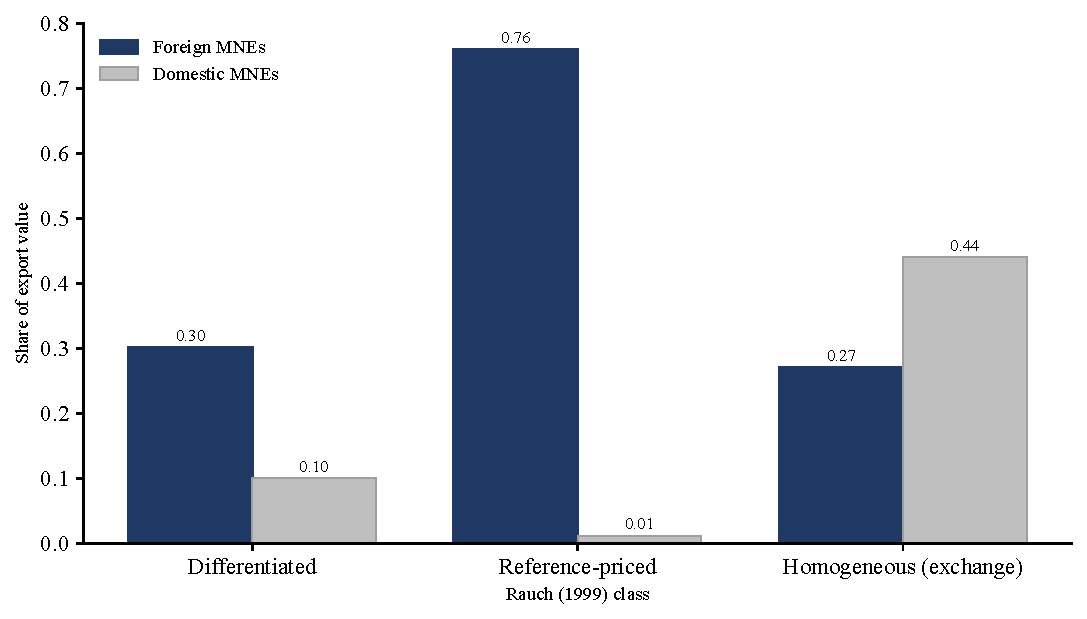
\includegraphics[width=0.7\textwidth,height=0.8\textheight,keepaspectratio]{figures/mining/fig_wp1b_rauch.pdf}%
  \caption{Mining and Fuels: Multinational Share of Export Value, by Rauch Product Class}%
  \label{fig:rauch_f_mining}%
  \par\vspace{2pt}%
  \parbox{0.92\textwidth}{\footnotesize %
  \textit{Notes:} Shares of mining and fuels export value (HS 25--27 and 71), all available years pooled. Rauch (1999) conservative classification: homogeneous goods are traded on organized exchanges, reference-priced goods have a price quoted in trade publications, and differentiated goods have neither.\\[3pt]%
  \textit{Source:} Authors' calculations based on customs data matched to Orbis and Dun \& Bradstreet.}%
  \end{figure}
% ---- Table: Mining and Fuels: Multinational Share of Export Value: Differentiated and Other Products
\begin{table}[H]\centering\small%
  \caption{Mining and Fuels: Multinational Share of Export Value: Differentiated and Other Products}%
  \label{tab:rauch2_mining}%
  \adjustbox{max width=\textwidth, max totalheight=0.8\textheight}{\begin{tabular}{lcccrr}
\toprule
Rauch (1999): differentiated vs non-differentiated & Foreign & Domestic & All MNEs & HS6 products & Value (US\$bn/yr) \\
\midrule
Differentiated & 0.301 & 0.100 & 0.401 & 40 & 0.3 \\
Non-differentiated & 0.464 & 0.270 & 0.734 & 126 & 64.6 \\
\bottomrule
\end{tabular}
}%
  \par\vspace{3pt}%
  \begin{minipage}{0.95\textwidth}\footnotesize %
  \textit{Notes:} Shares of mining and fuels export value (HS 25--27 and 71), all available years pooled. Rauch (1999) conservative classification; other products are reference-priced and homogeneous goods. Values are annual averages in US\$ billion.\\[3pt]%
  \textit{Source:} Authors' calculations based on customs data matched to Orbis and Dun \& Bradstreet.%
  \end{minipage}%
  \end{table}
% ---- Figure: Mining and Fuels: Multinational Share of Export Value: Differentiated and Other Products
\begin{figure}[H]\centering%
  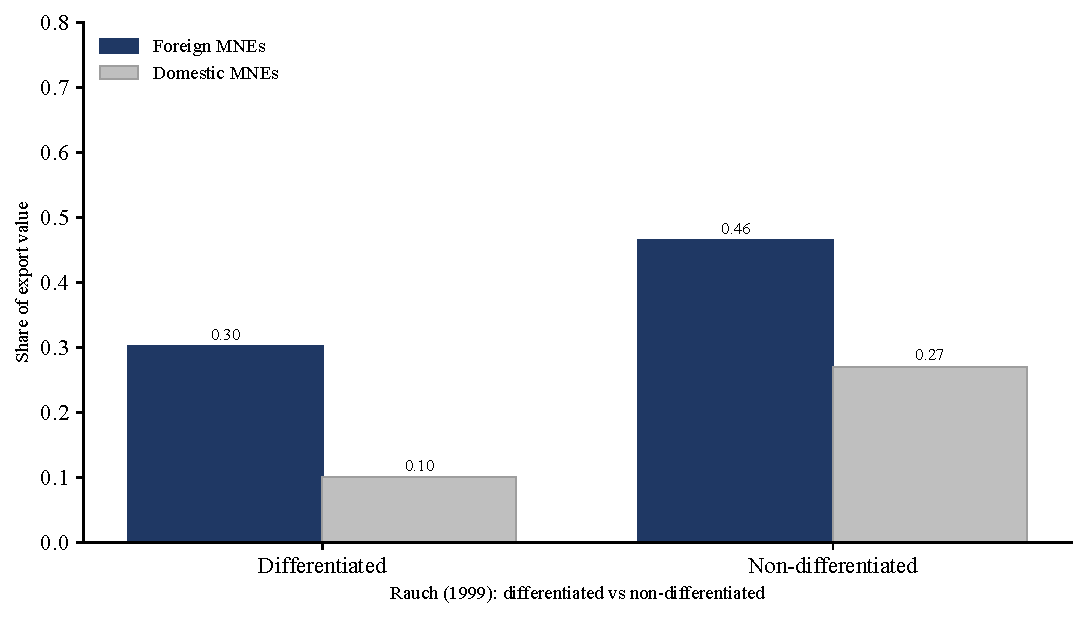
\includegraphics[width=0.7\textwidth,height=0.8\textheight,keepaspectratio]{figures/mining/fig_wp1b_rauch2.pdf}%
  \caption{Mining and Fuels: Multinational Share of Export Value: Differentiated and Other Products}%
  \label{fig:rauch2_f_mining}%
  \par\vspace{2pt}%
  \parbox{0.92\textwidth}{\footnotesize %
  \textit{Notes:} Shares of mining and fuels export value (HS 25--27 and 71), all available years pooled. Rauch (1999) conservative classification; other products are reference-priced and homogeneous goods.\\[3pt]%
  \textit{Source:} Authors' calculations based on customs data matched to Orbis and Dun \& Bradstreet.}%
  \end{figure}
% ---- Table: Mining and Fuels: Multinational Share of Export Value, by End Use
\begin{table}[H]\centering\small%
  \caption{Mining and Fuels: Multinational Share of Export Value, by End Use}%
  \label{tab:bec_mining}%
  \adjustbox{max width=\textwidth, max totalheight=0.8\textheight}{\begin{tabular}{lcccrr}
\toprule
BEC end use & Foreign & Domestic & All MNEs & HS6 products & Value (US\$bn/yr) \\
\midrule
Intermediate & 0.516 & 0.237 & 0.753 & 179 & 65.4 \\
Consumption & 0.617 & 0.004 & 0.621 & 11 & 0.5 \\
Capital & 0.214 & 0.000 & 0.214 & 2 & 0.0 \\
\bottomrule
\end{tabular}
}%
  \par\vspace{3pt}%
  \begin{minipage}{0.95\textwidth}\footnotesize %
  \textit{Notes:} Shares of mining and fuels export value (HS 25--27 and 71), all available years pooled. End use from BEC Rev.\,4; HS6 products without a BEC correspondence are excluded. Values are annual averages in US\$ billion.\\[3pt]%
  \textit{Source:} Authors' calculations based on customs data matched to Orbis and Dun \& Bradstreet.%
  \end{minipage}%
  \end{table}

\subsection{Regressions}
% ---- Table: Mining and Fuels: Product Characteristics and Multinational Shares
\begin{table}[H]\centering\small%
  \caption{Mining and Fuels: Product Characteristics and Multinational Shares}%
  \label{tab:fgo_r_mining}%
  \adjustbox{max width=\textwidth, max totalheight=0.8\textheight}{\begin{tabular}{lccc} \hline
 & (1) & (2) & (3) \\ \hline
\multicolumn{4}{l}{\textit{Panel A. Dependent variable: share of all MNEs}} \\
Complexity (PCI) & -0.1048*** & -0.0986*** & -0.0859*** \\
 & (0.0132) & (0.0120) & (0.0128) \\
$|\sigma|$ FGO (per s.d.) & 0.0156* & 0.0064 & -0.0016 \\
 & (0.0085) & (0.0087) & (0.0077) \\
Upstreamness & 0.1419*** & 0.1522*** & 0.1346*** \\
 & (0.0201) & (0.0194) & (0.0245) \\
\midrule
\multicolumn{4}{l}{\textit{Panel B. Dependent variable: share of foreign MNEs}} \\
Complexity (PCI) & 0.1307*** & 0.1349*** & 0.1174*** \\
 & (0.0134) & (0.0128) & (0.0136) \\
$|\sigma|$ FGO (per s.d.) & 0.1160*** & 0.1105*** & 0.1216*** \\
 & (0.0103) & (0.0098) & (0.0109) \\
Upstreamness & 0.0877*** & 0.0805*** & 0.0664*** \\
 & (0.0175) & (0.0173) & (0.0188) \\
\midrule
\multicolumn{4}{l}{\textit{Panel C. Dependent variable: share of domestic MNEs}} \\
Complexity (PCI) & -0.2355*** & -0.2335*** & -0.2033*** \\
 & (0.0124) & (0.0124) & (0.0149) \\
$|\sigma|$ FGO (per s.d.) & -0.1003*** & -0.1042*** & -0.1232*** \\
 & (0.0076) & (0.0079) & (0.0088) \\
Upstreamness & 0.0542*** & 0.0717*** & 0.0682*** \\
 & (0.0183) & (0.0183) & (0.0225) \\
\hline
Origin FE & $\checkmark$ &  &  \\
Destination FE & $\checkmark$ &  &  \\
Year FE & $\checkmark$ &  &  \\
Origin $\times$ year FE &  & $\checkmark$ &  \\
Destination $\times$ year FE &  & $\checkmark$ &  \\
Origin $\times$ dest.\ $\times$ year FE &  &  & $\checkmark$ \\
Observations & 23,906 & 23,513 & 22,358 \\
\hline
\end{tabular}
}%
  \par\vspace{3pt}%
  \begin{minipage}{0.95\textwidth}\footnotesize %
  \textit{Notes:} Observations are origin--destination--HS6--year cells. Mining and Fuels products only. Dependent variable: share of the cell's export value shipped by each type of MNE. The import-demand elasticity is standardized (mean 0, standard deviation 1). Regressions weighted by the cell's export value. Robust standard errors in parentheses. *** $p<0.01$, ** $p<0.05$, * $p<0.1$.\\[3pt]%
  \textit{Source:} Authors' calculations based on customs data matched to Orbis and Dun \& Bradstreet.%
  \end{minipage}%
  \end{table}
% ---- Table: Mining and Fuels: Product Sophistication and Multinational Shares
\begin{table}[H]\centering\footnotesize%
  \caption{Mining and Fuels: Product Sophistication and Multinational Shares}%
  \label{tab:meas_r_mining}%
  \adjustbox{max width=\textwidth, max totalheight=0.8\textheight}{\begin{tabular}{lcccccc} \hline
 & \multicolumn{2}{c}{PCI} & \multicolumn{2}{c}{Lall} & \multicolumn{2}{c}{Rauch} \\
 & (1) & (2) & (3) & (4) & (5) & (6) \\ \hline
\multicolumn{7}{l}{\textit{Panel A. Dependent variable: share of all MNEs}} \\
Complexity (PCI) & -0.1846*** & -0.1722*** &  &  &  &  \\
 & (0.0141) & (0.0166) &  &  &  &  \\
Lall: high tech (vs primary and resource-based) &  &  &  &  &  &  \\
 &  &  &  &  &  &  \\
Lall: medium tech &  &  &  &  &  &  \\
 &  &  &  &  &  &  \\
Lall: low tech &  &  & -0.3546*** & -0.3899*** &  &  \\
 &  &  & (0.0396) & (0.0501) &  &  \\
Rauch: differentiated (vs homogeneous) &  &  &  &  & -0.1843*** & -0.1742*** \\
 &  &  &  &  & (0.0457) & (0.0557) \\
Rauch: reference-priced &  &  &  &  & 0.1987*** & 0.2580*** \\
 &  &  &  &  & (0.0259) & (0.0351) \\
Observations & 32,084 & 30,880 & 32,087 & 30,883 & 24,732 & 23,549 \\
\midrule
\multicolumn{7}{l}{\textit{Panel B. Dependent variable: share of foreign MNEs}} \\
Complexity (PCI) & -0.0374** & -0.0647*** &  &  &  &  \\
 & (0.0169) & (0.0203) &  &  &  &  \\
Lall: high tech (vs primary and resource-based) &  &  &  &  &  &  \\
 &  &  &  &  &  &  \\
Lall: medium tech &  &  &  &  &  &  \\
 &  &  &  &  &  &  \\
Lall: low tech &  &  & -0.1503*** & -0.1296*** &  &  \\
 &  &  & (0.0248) & (0.0250) &  &  \\
Rauch: differentiated (vs homogeneous) &  &  &  &  & -0.0035 & -0.0015 \\
 &  &  &  &  & (0.0348) & (0.0435) \\
Rauch: reference-priced &  &  &  &  & 0.4411*** & 0.5010*** \\
 &  &  &  &  & (0.0211) & (0.0254) \\
Observations & 32,084 & 30,880 & 32,087 & 30,883 & 24,732 & 23,549 \\
\midrule
\multicolumn{7}{l}{\textit{Panel C. Dependent variable: share of domestic MNEs}} \\
Complexity (PCI) & -0.1472*** & -0.1075*** &  &  &  &  \\
 & (0.0173) & (0.0210) &  &  &  &  \\
Lall: high tech (vs primary and resource-based) &  &  &  &  &  &  \\
 &  &  &  &  &  &  \\
Lall: medium tech &  &  &  &  &  &  \\
 &  &  &  &  &  &  \\
Lall: low tech &  &  & -0.2044*** & -0.2602*** &  &  \\
 &  &  & (0.0457) & (0.0570) &  &  \\
Rauch: differentiated (vs homogeneous) &  &  &  &  & -0.1808*** & -0.1726*** \\
 &  &  &  &  & (0.0339) & (0.0410) \\
Rauch: reference-priced &  &  &  &  & -0.2423*** & -0.2430*** \\
 &  &  &  &  & (0.0237) & (0.0335) \\
Observations & 32,084 & 30,880 & 32,087 & 30,883 & 24,732 & 23,549 \\
\hline
Origin $\times$ year and destination $\times$ year FE & $\checkmark$ &  & $\checkmark$ &  & $\checkmark$ &  \\
Origin $\times$ dest.\ $\times$ year FE &  & $\checkmark$ &  & $\checkmark$ &  & $\checkmark$ \\
\hline
\end{tabular}
}%
  \par\vspace{3pt}%
  \begin{minipage}{0.95\textwidth}\footnotesize %
  \textit{Notes:} Observations are origin--destination--HS6--year cells. Mining and Fuels products only. Dependent variable: share of the cell's export value shipped by each type of MNE. Omitted categories: primary and resource-based products (Lall) and homogeneous products (Rauch). Robust standard errors in parentheses. *** $p<0.01$, ** $p<0.05$, * $p<0.1$.\\[3pt]%
  \textit{Source:} Authors' calculations based on customs data matched to Orbis and Dun \& Bradstreet.%
  \end{minipage}%
  \end{table}

\section{Fact 3: Multinationals from a Small Set of Countries Dominate Exports}\label{sec:f3_mining}

\subsection{Parent Countries}
% ---- Figure: Mining and Fuels: Foreign-Multinational Exports, by Parent Country
\begin{figure}[H]\centering%
  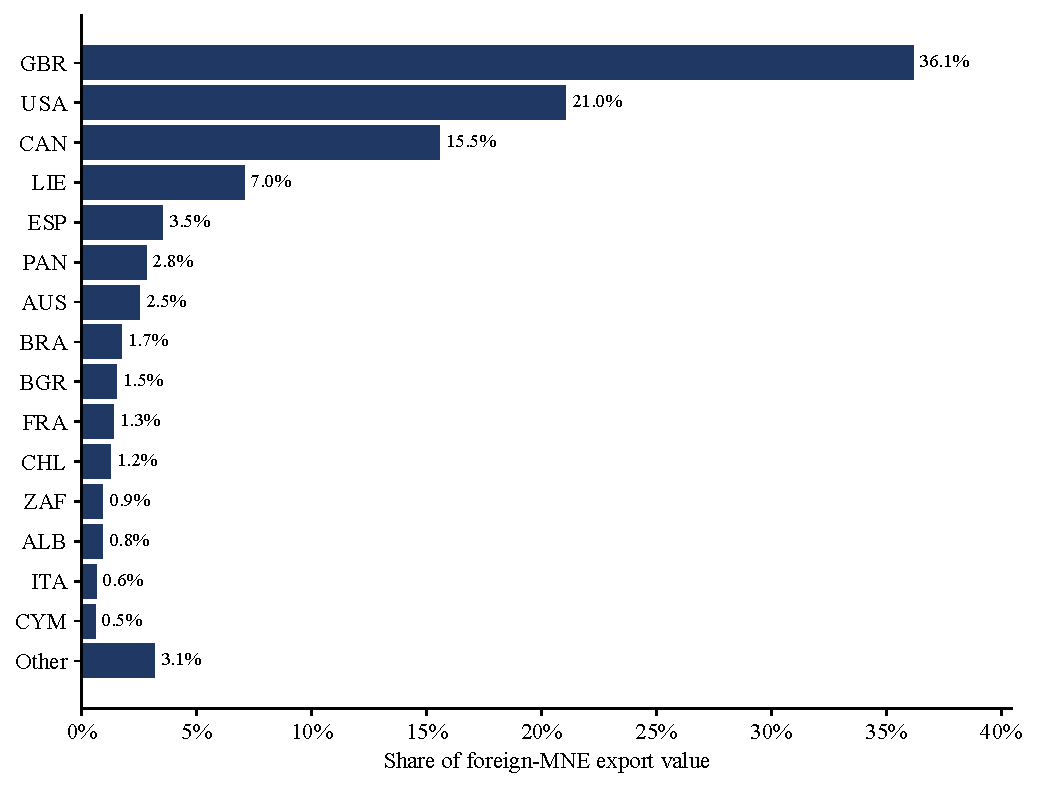
\includegraphics[width=0.78\textwidth,height=0.8\textheight,keepaspectratio]{figures/mining/fig_wp1a_parent_share.pdf}%
  \caption{Mining and Fuels: Foreign-Multinational Exports, by Parent Country}%
  \label{fig:f4_mining}%
  \par\vspace{2pt}%
  \parbox{0.92\textwidth}{\footnotesize %
  \textit{Notes:} Percent of foreign-MNE mining and fuels export value, by country of the ultimate parent.\\[3pt]%
  \textit{Source:} Authors' calculations based on customs data matched to Orbis and Dun \& Bradstreet.}%
  \end{figure}
% ---- Table: Mining and Fuels: Foreign-Multinational Exports, by Parent Country
\begin{table}[H]\centering\small%
  \caption{Mining and Fuels: Foreign-Multinational Exports, by Parent Country}%
  \label{tab:f4n_mining}%
  \adjustbox{max width=\textwidth, max totalheight=0.8\textheight}{\begin{tabular}{lrr}
\toprule
Parent country & Share (\%) & Value (US\$bn/yr) \\
\midrule
GBR & 36.1 & 11.9 \\
USA & 21.0 & 7.3 \\
CAN & 15.5 & 5.7 \\
LIE & 7.0 & 2.0 \\
ESP & 3.5 & 1.4 \\
PAN & 2.8 & 1.0 \\
AUS & 2.5 & 0.9 \\
BRA & 1.7 & 0.7 \\
BGR & 1.5 & 0.5 \\
FRA & 1.3 & 0.5 \\
CHL & 1.2 & 0.4 \\
ZAF & 0.9 & 0.3 \\
ALB & 0.8 & 0.3 \\
ITA & 0.6 & 0.2 \\
CYM & 0.5 & 0.2 \\
Other (87 countries) & 3.1 & 1.2 \\
\midrule
All foreign MNEs & 100.0 & 36.0 \\
\bottomrule
\end{tabular}
}%
  \par\vspace{3pt}%
  \begin{minipage}{0.95\textwidth}\footnotesize %
  \textit{Notes:} Percent of foreign-MNE mining and fuels export value, by country of the ultimate parent. Values are annual averages in US\$ billion.\\[3pt]%
  \textit{Source:} Authors' calculations based on customs data matched to Orbis and Dun \& Bradstreet.%
  \end{minipage}%
  \end{table}
% ---- Figure: Mining and Fuels: Share of Total Exports, by Parent Country
\begin{figure}[H]\centering%
  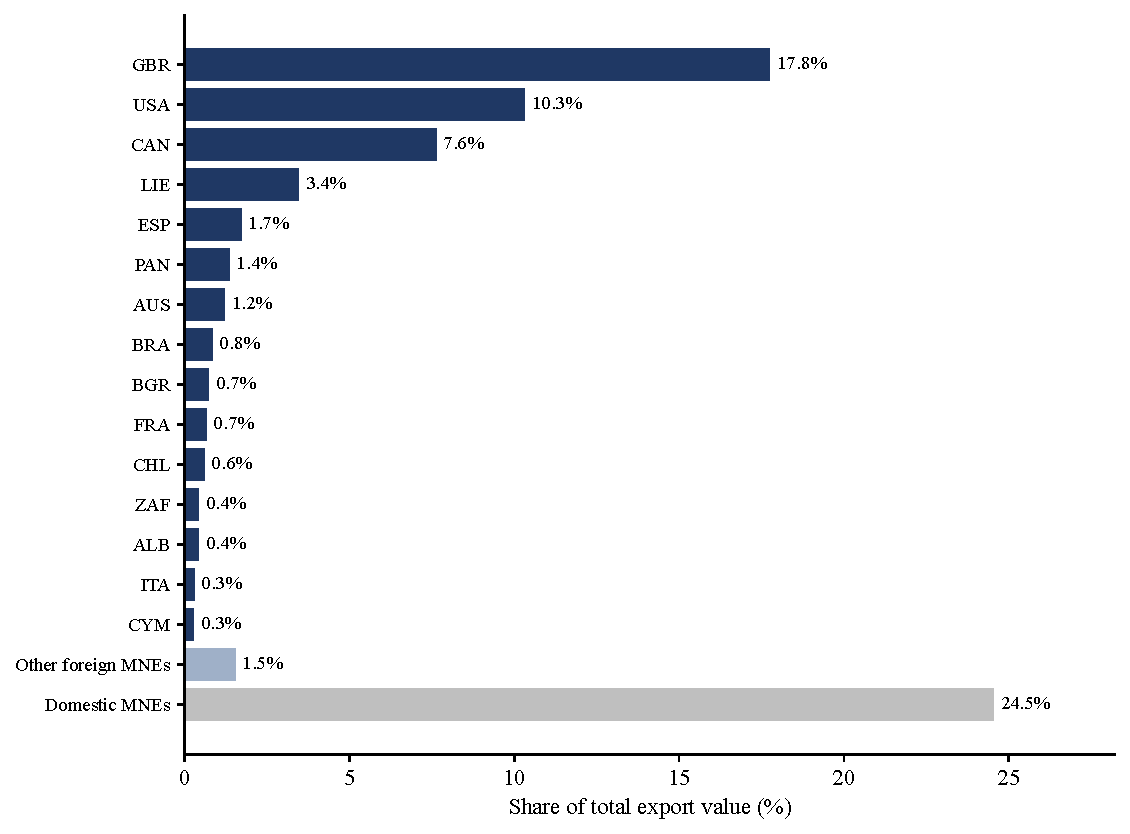
\includegraphics[width=0.85\textwidth,height=0.8\textheight,keepaspectratio]{figures/mining/fig_wp1a_parent_share_total.pdf}%
  \caption{Mining and Fuels: Share of Total Exports, by Parent Country}%
  \label{fig:f4t_mining}%
  \par\vspace{2pt}%
  \parbox{0.92\textwidth}{\footnotesize %
  \textit{Notes:} Percent of total mining and fuels export value shipped by foreign MNEs of each parent country, other foreign MNEs and domestic MNEs; the remainder is local firms.\\[3pt]%
  \textit{Source:} Authors' calculations based on customs data matched to Orbis and Dun \& Bradstreet.}%
  \end{figure}
% ---- Table: Mining and Fuels: Share of Total Exports, by Parent Country
\begin{table}[H]\centering\small%
  \caption{Mining and Fuels: Share of Total Exports, by Parent Country}%
  \label{tab:f4tn_mining}%
  \adjustbox{max width=\textwidth, max totalheight=0.8\textheight}{\begin{tabular}{lr}
\toprule
Exporter type / parent country & Share of total exports (\%) \\
\midrule
GBR & 17.8 \\
USA & 10.3 \\
CAN & 7.6 \\
LIE & 3.4 \\
ESP & 1.7 \\
PAN & 1.4 \\
AUS & 1.2 \\
BRA & 0.8 \\
BGR & 0.7 \\
FRA & 0.7 \\
CHL & 0.6 \\
ZAF & 0.4 \\
ALB & 0.4 \\
ITA & 0.3 \\
CYM & 0.3 \\
Other foreign MNEs & 1.5 \\
Domestic MNEs & 24.5 \\
\midrule
All MNEs & 73.7 \\
Local firms & 26.3 \\
\bottomrule
\end{tabular}
}%
  \par\vspace{3pt}%
  \begin{minipage}{0.95\textwidth}\footnotesize %
  \textit{Notes:} Percent of total mining and fuels export value, by type of exporter and parent country.\\[3pt]%
  \textit{Source:} Authors' calculations based on customs data matched to Orbis and Dun \& Bradstreet.%
  \end{minipage}%
  \end{table}

\subsection{Parent Region and Destination Region}
% ---- Table: Mining and Fuels: Multinational Exports by Parent Region and Destination Region: Export Value
\begin{table}[H]\centering\small%
  \caption{Mining and Fuels: Multinational Exports by Parent Region and Destination Region: Export Value}%
  \label{tab:reg_value_mining}%
  \adjustbox{max width=\textwidth, max totalheight=0.8\textheight}{\begin{tabular}{lrrrrrrrr}
\toprule
Parent region / Destination region & Latin America & North America & Europe & Asia & Africa & Oceania & Rest of World & Total \\
\midrule
Latin America & 0.6 & 0.4 & 0.6 & 0.9 & 0.0 & 0.1 & 0.0 & 2.6 \\
North America & 1.7 & 2.9 & 4.5 & 3.9 & 0.0 & 0.0 & 0.0 & 13.0 \\
Europe & 2.2 & 2.0 & 3.5 & 9.5 & 0.2 & 0.0 & 0.0 & 17.3 \\
Asia & 0.0 & 0.1 & 0.0 & 0.1 & 0.0 & 0.0 & 0.0 & 0.2 \\
Africa & 0.0 & 0.0 & 0.2 & 0.2 & 0.0 & 0.0 & 0.0 & 0.4 \\
Oceania & 0.2 & 0.0 & 0.1 & 0.7 & 0.0 & 0.0 & 0.0 & 0.9 \\
Rest of World & 0.0 & 0.0 & 0.0 & 0.0 & 0.0 & 0.0 & 0.0 & 0.0 \\
Domestic MNEs & 3.7 & 7.4 & 1.1 & 4.1 & 0.2 & 0.0 & 0.1 & 16.5 \\
Local firms & 3.5 & 5.9 & 4.9 & 5.3 & 0.1 & 0.0 & 0.2 & 19.9 \\
\midrule
Total & 11.9 & 18.7 & 14.8 & 24.6 & 0.5 & 0.1 & 0.3 & 71.0 \\
\bottomrule
\end{tabular}
}%
  \par\vspace{3pt}%
  \begin{minipage}{0.95\textwidth}\footnotesize %
  \textit{Notes:} Values are annual averages in US\$ billion. Rows: region of the ultimate parent; columns: destination region.\\[3pt]%
  \textit{Source:} Authors' calculations based on customs data matched to Orbis and Dun \& Bradstreet.%
  \end{minipage}%
  \end{table}
% ---- Table: Mining and Fuels: Multinational Exports by Parent Region and Destination Region: Row Percentages
\begin{table}[H]\centering\small%
  \caption{Mining and Fuels: Multinational Exports by Parent Region and Destination Region: Row Percentages}%
  \label{tab:reg_rowpct_mining}%
  \adjustbox{max width=\textwidth, max totalheight=0.8\textheight}{\begin{tabular}{lrrrrrrrr}
\toprule
Parent region / Destination region & Latin America & North America & Europe & Asia & Africa & Oceania & Rest of World & Total \\
\midrule
Latin America & 24.6 & 16.6 & 22.3 & 33.8 & 0.0 & 2.4 & 0.2 & 100.0 \\
North America & 14.3 & 20.7 & 35.0 & 29.8 & 0.2 & 0.0 & 0.0 & 100.0 \\
Europe & 11.5 & 9.9 & 19.4 & 58.0 & 0.9 & 0.1 & 0.2 & 100.0 \\
Asia & 5.8 & 32.7 & 15.1 & 45.6 & 0.1 & 0.3 & 0.4 & 100.0 \\
Africa & 0.7 & 3.7 & 35.6 & 58.6 & 1.4 & 0.0 & 0.1 & 100.0 \\
Oceania & 16.6 & 4.2 & 7.4 & 71.7 & 0.0 & 0.0 & 0.0 & 100.0 \\
Rest of World & 100.0 & 0.0 & 0.0 & 0.0 & 0.0 & 0.0 & 0.0 & 100.0 \\
Domestic MNEs & 22.1 & 44.4 & 6.8 & 25.3 & 1.0 & 0.0 & 0.4 & 100.0 \\
Local firms & 17.5 & 29.2 & 24.8 & 26.9 & 0.5 & 0.1 & 1.1 & 100.0 \\
\bottomrule
\end{tabular}
}%
  \par\vspace{3pt}%
  \begin{minipage}{0.95\textwidth}\footnotesize %
  \textit{Notes:} Percent of each group's exports, by destination region (rows add to 100). Domestic MNEs and local firms are shown for comparison.\\[3pt]%
  \textit{Source:} Authors' calculations based on customs data matched to Orbis and Dun \& Bradstreet.%
  \end{minipage}%
  \end{table}
% ---- Table: Mining and Fuels: Multinational Exports by Parent Region and Destination Region: Column Percentages
\begin{table}[H]\centering\small%
  \caption{Mining and Fuels: Multinational Exports by Parent Region and Destination Region: Column Percentages}%
  \label{tab:reg_colpct_mining}%
  \adjustbox{max width=\textwidth, max totalheight=0.8\textheight}{\begin{tabular}{lrrrrrrr}
\toprule
Parent region / Destination region & Latin America & North America & Europe & Asia & Africa & Oceania & Rest of World \\
\midrule
Latin America & 5.0 & 2.2 & 3.7 & 3.2 & 0.1 & 51.7 & 1.9 \\
North America & 15.0 & 14.1 & 30.1 & 14.6 & 5.6 & 2.4 & 0.7 \\
Europe & 17.4 & 9.7 & 23.8 & 40.7 & 35.1 & 21.0 & 9.2 \\
Asia & 0.1 & 0.4 & 0.2 & 0.4 & 0.0 & 0.6 & 0.3 \\
Africa & 0.0 & 0.1 & 0.9 & 0.9 & 1.1 & 0.0 & 0.2 \\
Oceania & 1.2 & 0.2 & 0.4 & 2.4 & 0.0 & 0.1 & 0.0 \\
Rest of World & 0.0 & 0.0 & 0.0 & 0.0 & 0.0 & 0.0 & 0.0 \\
Domestic MNEs & 33.2 & 43.0 & 8.3 & 17.7 & 39.1 & 2.2 & 22.3 \\
Local firms & 28.1 & 30.3 & 32.5 & 20.1 & 19.0 & 22.0 & 65.4 \\
\midrule
Total & 100.0 & 100.0 & 100.0 & 100.0 & 100.0 & 100.0 & 100.0 \\
\bottomrule
\end{tabular}
}%
  \par\vspace{3pt}%
  \begin{minipage}{0.95\textwidth}\footnotesize %
  \textit{Notes:} Percent of the exports reaching each destination region, by parent region (columns add to 100).\\[3pt]%
  \textit{Source:} Authors' calculations based on customs data matched to Orbis and Dun \& Bradstreet.%
  \end{minipage}%
  \end{table}
% ---- Figure: Mining and Fuels: Multinational Exports by Parent Region and Destination Region
\begin{figure}[H]\centering%
  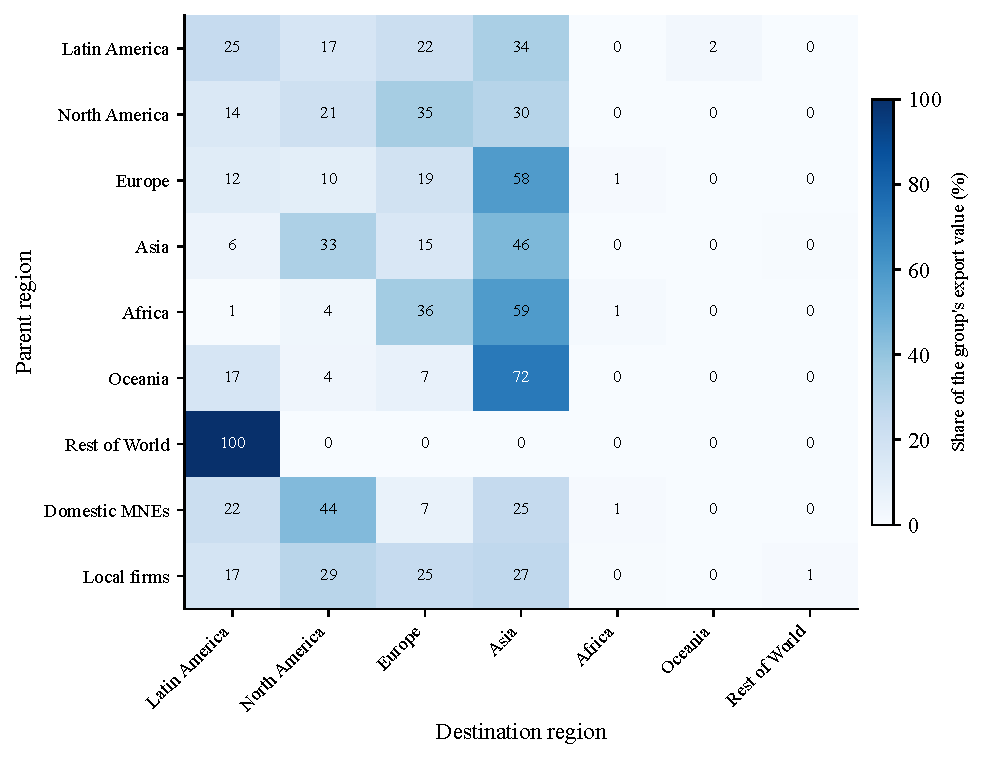
\includegraphics[width=0.9\textwidth,height=0.8\textheight,keepaspectratio]{figures/mining/fig_wp1d_heatmap_region_rowpct.pdf}%
  \caption{Mining and Fuels: Multinational Exports by Parent Region and Destination Region}%
  \label{fig:reg_hm_mining}%
  \par\vspace{2pt}%
  \parbox{0.92\textwidth}{\footnotesize %
  \textit{Notes:} Percent of each group's exports, by destination region (rows add to 100).\\[3pt]%
  \textit{Source:} Authors' calculations based on customs data matched to Orbis and Dun \& Bradstreet.}%
  \end{figure}
% ---- Table: Mining and Fuels: Foreign-Multinational Exports by Exporting Country and Destination Region
\begin{table}[H]\centering\small%
  \caption{Mining and Fuels: Foreign-Multinational Exports by Exporting Country and Destination Region}%
  \label{tab:odr_f_mining}%
  \adjustbox{max width=\textwidth, max totalheight=0.8\textheight}{\begin{tabular}{lrrrrrrrr}
\toprule
Origin \ Destination region & Latin America & North America & Europe & Asia & Africa & Oceania & Rest of World & Total \\
\midrule
ARG & 18.8 & 37.6 & 25.9 & 17.2 & 0.4 & 0.1 & 0.1 & 5.0 \\
CHL & 3.2 & 3.2 & 12.9 & 80.5 & 0.1 & 0.1 & 0.0 & 7.5 \\
COL & 29.4 & 18.2 & 37.2 & 13.8 & 0.5 & 0.2 & 0.6 & 8.4 \\
CRI & 76.5 & 23.1 & 0.3 & 0.1 & 0.0 & 0.0 & 0.0 & 0.1 \\
DOM & 4.4 & 56.9 & 13.5 & 25.1 & 0.0 & 0.0 & 0.0 & 1.7 \\
PER & 10.0 & 8.8 & 25.3 & 54.4 & 1.0 & 0.5 & 0.0 & 13.2 \\
PRY & 46.0 & 21.2 & 32.7 & 0.0 & 0.0 & 0.0 & 0.0 & 0.0 \\
SLV & 92.4 & 6.0 & 1.5 & 0.1 & 0.0 & 0.0 & 0.0 & 0.1 \\
URY & 12.5 & 1.8 & 80.1 & 5.1 & 0.1 & 0.0 & 0.3 & 0.1 \\
\bottomrule
\end{tabular}
}%
  \par\vspace{3pt}%
  \begin{minipage}{0.95\textwidth}\footnotesize %
  \textit{Notes:} Percent of each country's foreign-MNE mining and fuels exports, by destination region (rows add to 100). Last column: foreign-MNE exports. Values are annual averages in US\$ billion.\\[3pt]%
  \textit{Source:} Authors' calculations based on customs data matched to Orbis and Dun \& Bradstreet.%
  \end{minipage}%
  \end{table}
% ---- Table: Mining and Fuels: Local-Firm Exports by Exporting Country and Destination Region
\begin{table}[H]\centering\small%
  \caption{Mining and Fuels: Local-Firm Exports by Exporting Country and Destination Region}%
  \label{tab:odr_l_mining}%
  \adjustbox{max width=\textwidth, max totalheight=0.8\textheight}{\begin{tabular}{lrrrrrrrr}
\toprule
Origin \ Destination region & Latin America & North America & Europe & Asia & Africa & Oceania & Rest of World & Total \\
\midrule
ARG & 53.6 & 12.4 & 28.5 & 3.3 & 1.9 & 0.4 & 0.0 & 1.6 \\
CHL & 12.3 & 8.5 & 25.3 & 53.3 & 0.4 & 0.2 & 0.0 & 1.9 \\
COL & 23.5 & 35.2 & 28.3 & 9.0 & 0.5 & 0.0 & 3.5 & 4.1 \\
CRI & 19.3 & 74.7 & 4.6 & 1.4 & 0.0 & 0.0 & 0.0 & 0.1 \\
DOM & 36.7 & 56.6 & 2.1 & 0.0 & 4.5 & 0.0 & 0.0 & 0.3 \\
PER & 10.3 & 32.7 & 23.8 & 32.4 & 0.2 & 0.1 & 0.5 & 11.8 \\
PRY & 85.2 & 13.0 & 1.0 & 0.7 & 0.0 & 0.0 & 0.0 & 0.0 \\
SLV & 41.3 & 58.1 & 0.1 & 0.5 & 0.0 & 0.0 & 0.0 & 0.1 \\
URY & 83.9 & 5.4 & 1.1 & 9.5 & 0.0 & 0.1 & 0.0 & 0.1 \\
\bottomrule
\end{tabular}
}%
  \par\vspace{3pt}%
  \begin{minipage}{0.95\textwidth}\footnotesize %
  \textit{Notes:} Percent of each country's mining and fuels exports by local firms, by destination region (rows add to 100). Last column: local-firm exports. Values are annual averages in US\$ billion.\\[3pt]%
  \textit{Source:} Authors' calculations based on customs data matched to Orbis and Dun \& Bradstreet.%
  \end{minipage}%
  \end{table}

\subsection{Parent Country and Destination Country}
% ---- Table: Mining and Fuels: Foreign-Multinational Exports by Parent Country and Destination: Export Value
\begin{table}[H]\centering\small%
  \caption{Mining and Fuels: Foreign-Multinational Exports by Parent Country and Destination: Export Value}%
  \label{tab:cty_value_mining}%
  \adjustbox{max width=\textwidth, max totalheight=0.8\textheight}{\begin{tabular}{lrrrrrrrrrrrr}
\toprule
Parent / Destination & CHN & JPN & USA & CAN & CHE & KOR & ESP & IND & DEU & CHL & Other destinations & Total \\
\midrule
GBR & 4.5 & 1.1 & 0.2 & 0.3 & 0.1 & 0.8 & 0.5 & 0.6 & 0.7 & 0.5 & 2.5 & 11.9 \\
USA & 1.1 & 0.7 & 0.9 & 0.0 & 0.5 & 0.3 & 0.8 & 0.1 & 0.1 & 0.2 & 2.6 & 7.3 \\
CAN & 0.4 & 0.3 & 0.3 & 1.7 & 1.1 & 0.1 & 0.2 & 0.4 & 0.2 & 0.0 & 1.0 & 5.7 \\
LIE & 0.6 & 0.7 & 0.0 & 0.0 & 0.0 & 0.2 & 0.1 & 0.1 & 0.0 & 0.1 & 0.2 & 2.0 \\
ESP & 0.4 & 0.0 & 0.6 & 0.0 & 0.0 & 0.0 & 0.0 & 0.0 & 0.0 & 0.1 & 0.3 & 1.4 \\
PAN & 0.4 & 0.0 & 0.1 & 0.0 & 0.0 & 0.1 & 0.0 & 0.0 & 0.0 & 0.0 & 0.3 & 1.0 \\
AUS & 0.3 & 0.1 & 0.0 & 0.0 & 0.0 & 0.1 & 0.0 & 0.1 & 0.0 & 0.0 & 0.2 & 0.9 \\
BRA & 0.0 & 0.0 & 0.1 & 0.0 & 0.1 & 0.0 & 0.0 & 0.0 & 0.0 & 0.0 & 0.4 & 0.7 \\
BGR & 0.0 & 0.0 & 0.2 & 0.0 & 0.0 & 0.0 & 0.0 & 0.0 & 0.0 & 0.0 & 0.2 & 0.5 \\
FRA & 0.1 & 0.0 & 0.1 & 0.0 & 0.0 & 0.0 & 0.0 & 0.0 & 0.0 & 0.1 & 0.3 & 0.5 \\
Other parents & 0.3 & 0.1 & 0.5 & 0.2 & 0.2 & 0.1 & 0.1 & 0.1 & 0.1 & 0.1 & 0.8 & 2.6 \\
\midrule
Total & 8.2 & 3.1 & 3.1 & 2.3 & 2.0 & 1.6 & 1.7 & 1.5 & 1.2 & 1.2 & 8.7 & 34.5 \\
\bottomrule
\end{tabular}
}%
  \par\vspace{3pt}%
  \begin{minipage}{0.95\textwidth}\footnotesize %
  \textit{Notes:} Values are annual averages in US\$ billion. Ten largest parent countries and ten largest destinations by foreign-MNE export value.\\[3pt]%
  \textit{Source:} Authors' calculations based on customs data matched to Orbis and Dun \& Bradstreet.%
  \end{minipage}%
  \end{table}
% ---- Table: Mining and Fuels: Foreign-Multinational Exports by Parent Country and Destination: Row Percentages
\begin{table}[H]\centering\small%
  \caption{Mining and Fuels: Foreign-Multinational Exports by Parent Country and Destination: Row Percentages}%
  \label{tab:cty_rowpct_mining}%
  \adjustbox{max width=\textwidth, max totalheight=0.8\textheight}{\begin{tabular}{lrrrrrrrrrrrr}
\toprule
Parent / Destination & CHN & JPN & USA & CAN & CHE & KOR & ESP & IND & DEU & CHL & Other destinations & Total \\
\midrule
GBR & 38.8 & 9.8 & 1.9 & 2.6 & 0.9 & 6.4 & 3.8 & 5.6 & 4.8 & 4.2 & 21.1 & 100.0 \\
USA & 15.0 & 9.0 & 12.5 & 0.6 & 5.1 & 4.6 & 10.7 & 1.7 & 0.8 & 2.4 & 37.8 & 100.0 \\
CAN & 8.2 & 6.7 & 4.9 & 26.1 & 17.5 & 1.1 & 3.4 & 6.5 & 4.7 & 0.3 & 20.5 & 100.0 \\
LIE & 31.9 & 38.0 & 1.1 & 0.0 & 0.4 & 8.2 & 2.7 & 4.5 & 1.7 & 3.2 & 8.2 & 100.0 \\
ESP & 26.5 & 0.0 & 37.6 & 0.3 & 0.3 & 0.4 & 3.4 & 3.1 & 0.0 & 8.4 & 20.0 & 100.0 \\
PAN & 38.3 & 1.5 & 8.0 & 0.9 & 0.5 & 10.8 & 1.8 & 3.5 & 3.3 & 0.2 & 31.1 & 100.0 \\
AUS & 35.3 & 14.3 & 2.1 & 2.1 & 3.8 & 11.4 & 2.1 & 6.7 & 0.8 & 2.3 & 19.3 & 100.0 \\
BRA & 1.2 & 0.7 & 22.4 & 0.1 & 8.6 & 1.0 & 0.2 & 7.3 & 0.0 & 2.5 & 56.1 & 100.0 \\
BGR & 5.5 & 0.0 & 50.6 & 0.0 & 0.0 & 0.0 & 5.6 & 1.2 & 0.2 & 0.0 & 36.8 & 100.0 \\
FRA & 13.9 & 1.0 & 14.0 & 0.4 & 0.9 & 2.7 & 1.0 & 0.9 & 0.6 & 10.5 & 54.1 & 100.0 \\
Other parents & 10.2 & 4.9 & 20.7 & 7.4 & 7.6 & 3.0 & 2.7 & 3.6 & 4.8 & 4.0 & 31.2 & 100.0 \\
\bottomrule
\end{tabular}
}%
  \par\vspace{3pt}%
  \begin{minipage}{0.95\textwidth}\footnotesize %
  \textit{Notes:} Percent of each parent country's exports, by destination (rows add to 100). Ten largest parent countries and destinations.\\[3pt]%
  \textit{Source:} Authors' calculations based on customs data matched to Orbis and Dun \& Bradstreet.%
  \end{minipage}%
  \end{table}
% ---- Table: Mining and Fuels: Foreign-Multinational Exports by Parent Country and Destination: Column Percentages
\begin{table}[H]\centering\small%
  \caption{Mining and Fuels: Foreign-Multinational Exports by Parent Country and Destination: Column Percentages}%
  \label{tab:cty_colpct_mining}%
  \adjustbox{max width=\textwidth, max totalheight=0.8\textheight}{\begin{tabular}{lrrrrrrrrrrr}
\toprule
Parent / Destination & CHN & JPN & USA & CAN & CHE & KOR & ESP & IND & DEU & CHL & Other destinations \\
\midrule
GBR & 57.1 & 35.9 & 8.0 & 16.6 & 6.7 & 47.4 & 28.2 & 45.3 & 53.8 & 48.9 & 29.6 \\
USA & 12.8 & 19.0 & 30.8 & 2.1 & 21.5 & 19.7 & 46.3 & 8.0 & 5.2 & 15.9 & 30.8 \\
CAN & 5.2 & 10.5 & 9.0 & 70.6 & 54.8 & 3.5 & 11.0 & 22.4 & 22.6 & 1.7 & 12.3 \\
LIE & 9.1 & 26.9 & 0.9 & 0.0 & 0.6 & 11.8 & 3.9 & 7.0 & 3.7 & 7.3 & 2.2 \\
ESP & 3.8 & 0.0 & 15.4 & 0.2 & 0.2 & 0.3 & 2.4 & 2.4 & 0.0 & 9.4 & 2.7 \\
PAN & 4.3 & 0.4 & 2.6 & 0.4 & 0.3 & 6.1 & 1.0 & 2.2 & 2.9 & 0.2 & 3.3 \\
AUS & 3.5 & 3.6 & 0.6 & 0.9 & 1.9 & 5.7 & 1.0 & 3.6 & 0.6 & 1.8 & 1.8 \\
BRA & 0.1 & 0.1 & 4.4 & 0.0 & 2.9 & 0.3 & 0.1 & 2.7 & 0.0 & 1.3 & 3.7 \\
BGR & 0.3 & 0.0 & 8.7 & 0.0 & 0.0 & 0.0 & 1.7 & 0.4 & 0.1 & 0.0 & 2.1 \\
FRA & 0.8 & 0.1 & 2.2 & 0.1 & 0.2 & 0.7 & 0.3 & 0.3 & 0.2 & 4.5 & 2.8 \\
Other parents & 3.0 & 3.5 & 17.4 & 9.1 & 10.9 & 4.4 & 4.0 & 5.8 & 10.8 & 9.1 & 8.7 \\
\midrule
Total & 100.0 & 100.0 & 100.0 & 100.0 & 100.0 & 100.0 & 100.0 & 100.0 & 100.0 & 100.0 & 100.0 \\
\bottomrule
\end{tabular}
}%
  \par\vspace{3pt}%
  \begin{minipage}{0.95\textwidth}\footnotesize %
  \textit{Notes:} Percent of the foreign-MNE exports reaching each destination, by parent country (columns add to 100). Ten largest parent countries and destinations.\\[3pt]%
  \textit{Source:} Authors' calculations based on customs data matched to Orbis and Dun \& Bradstreet.%
  \end{minipage}%
  \end{table}
% ---- Figure: Mining and Fuels: Destination of Foreign-Multinational Exports: Fifteen Largest Parent Countries and Destinations
\begin{figure}[H]\centering%
  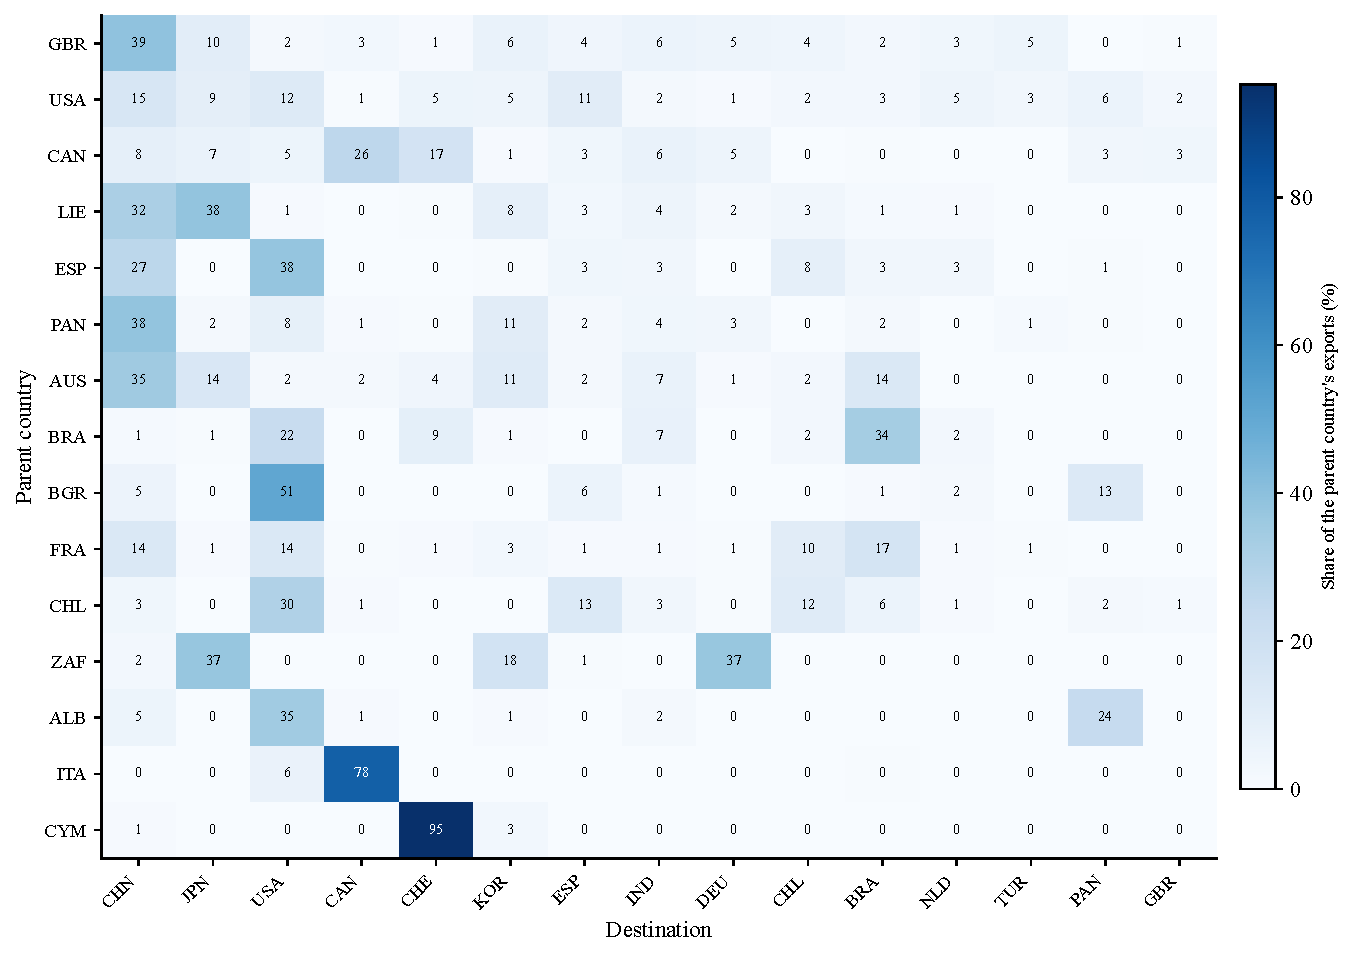
\includegraphics[width=1.0\textwidth,height=0.8\textheight,keepaspectratio]{figures/mining/fig_wp1d_heatmap_country_rowpct.pdf}%
  \caption{Mining and Fuels: Destination of Foreign-Multinational Exports: Fifteen Largest Parent Countries and Destinations}%
  \label{fig:hm_row_mining}%
  \par\vspace{2pt}%
  \parbox{0.92\textwidth}{\footnotesize %
  \textit{Notes:} Percent of each parent country's exports going to each destination (rows add to 100 including other destinations).\\[3pt]%
  \textit{Source:} Authors' calculations based on customs data matched to Orbis and Dun \& Bradstreet.}%
  \end{figure}
% ---- Figure: Mining and Fuels: Foreign-Multinational Exports by Parent Country and Destination: Share of the Total
\begin{figure}[H]\centering%
  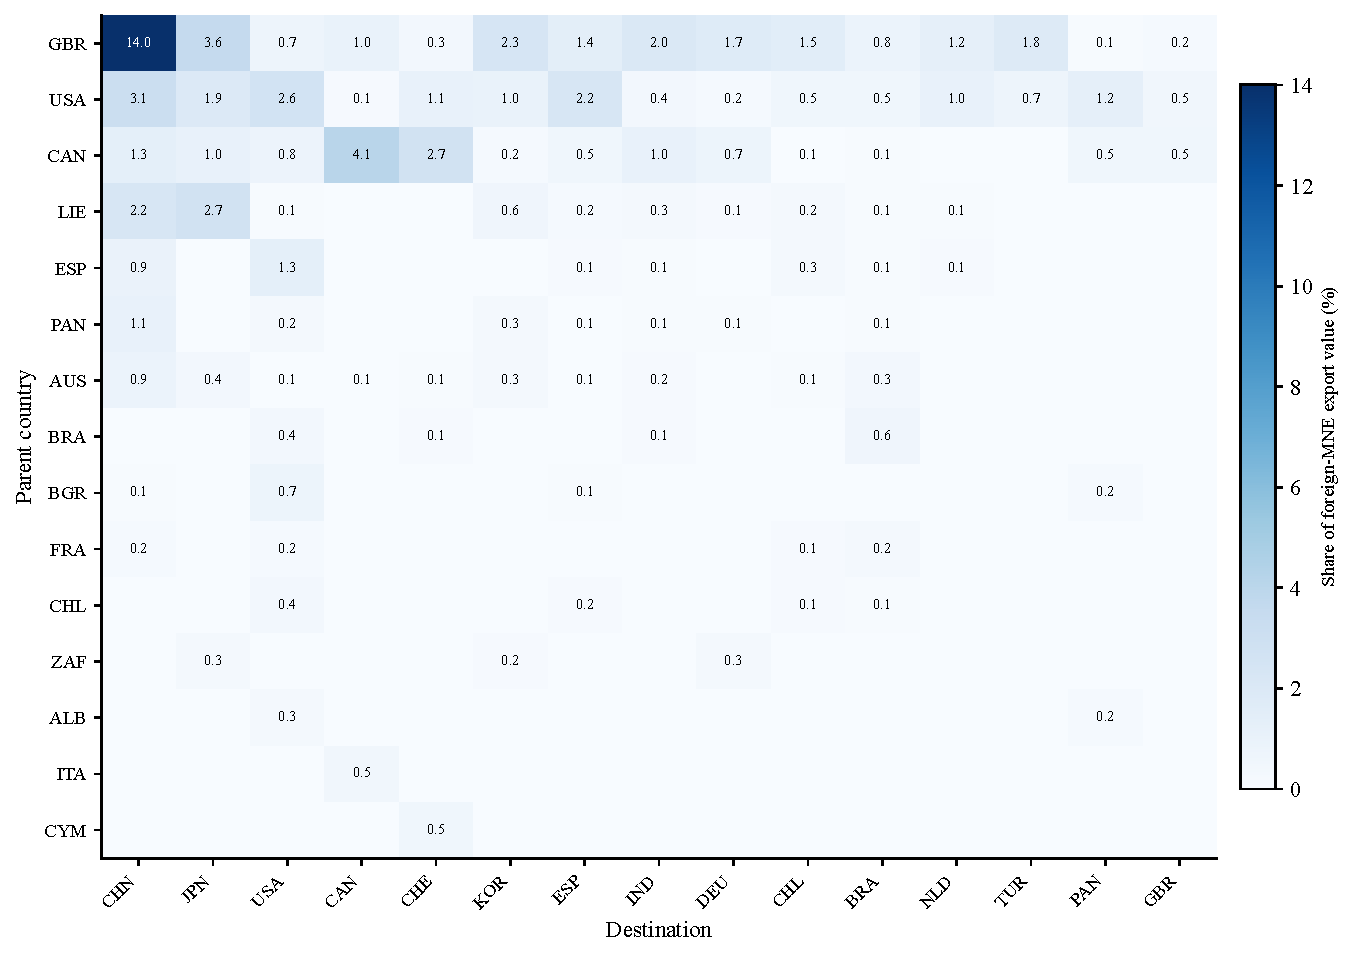
\includegraphics[width=1.0\textwidth,height=0.8\textheight,keepaspectratio]{figures/mining/fig_wp1d_heatmap_country_cellpct.pdf}%
  \caption{Mining and Fuels: Foreign-Multinational Exports by Parent Country and Destination: Share of the Total}%
  \label{fig:hm_cell_mining}%
  \par\vspace{2pt}%
  \parbox{0.92\textwidth}{\footnotesize %
  \textit{Notes:} Percent of all foreign-MNE export value in each parent country and destination pair; fifteen largest parent countries and destinations.\\[3pt]%
  \textit{Source:} Authors' calculations based on customs data matched to Orbis and Dun \& Bradstreet.}%
  \end{figure}

\subsection{Exports to the Parent Country}
% ---- Figure: Mining and Fuels: Share of Foreign-Multinational Exports Shipped to the Parent Country
\begin{figure}[H]\centering%
  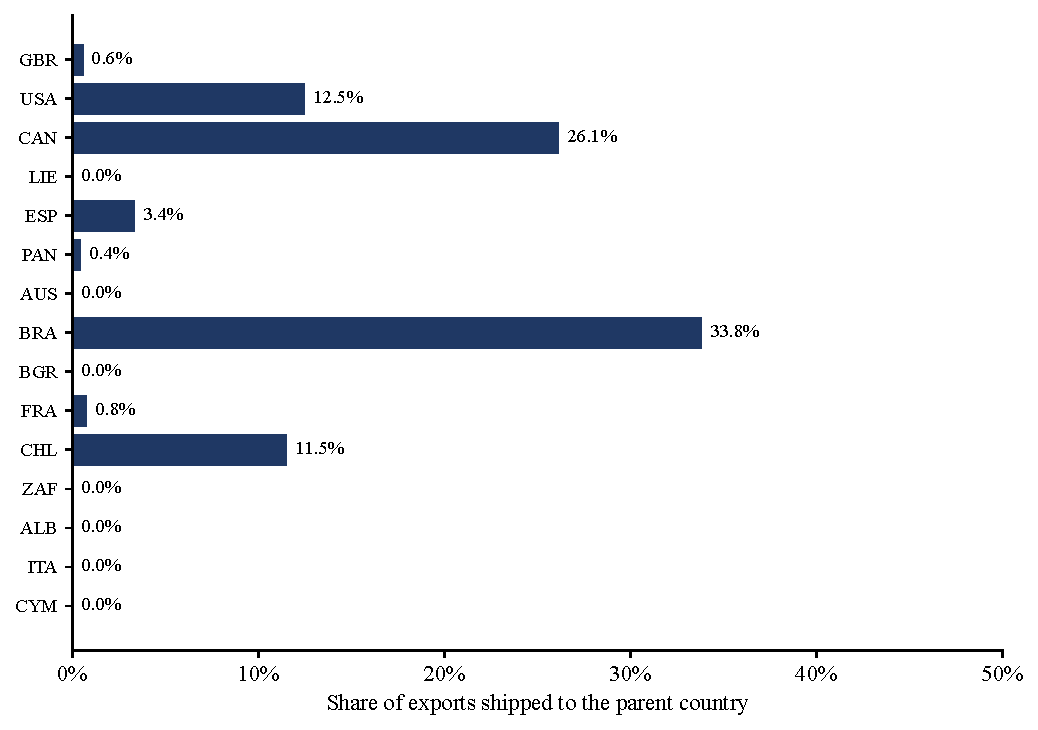
\includegraphics[width=0.85\textwidth,height=0.8\textheight,keepaspectratio]{figures/mining/fig_wp1d_home_share_by_parent.pdf}%
  \caption{Mining and Fuels: Share of Foreign-Multinational Exports Shipped to the Parent Country}%
  \label{fig:home_mining}%
  \par\vspace{2pt}%
  \parbox{0.92\textwidth}{\footnotesize %
  \textit{Notes:} Percent of each parent country's exports shipped to that same country.\\[3pt]%
  \textit{Source:} Authors' calculations based on customs data matched to Orbis and Dun \& Bradstreet.}%
  \end{figure}
% ---- Table: Mining and Fuels: Foreign-Multinational Exports to the Parent Countries, by Parent Country
\begin{table}[H]\centering\small%
  \caption{Mining and Fuels: Foreign-Multinational Exports to the Parent Countries, by Parent Country}%
  \label{tab:pxp_mining}%
  \adjustbox{max width=\textwidth, max totalheight=0.8\textheight}{\begin{tabular}{lrrrrrrrrrrr}
\toprule
Parent / Destination & GBR & USA & CAN & ESP & PAN & AUS & BRA & BGR & FRA & Other destinations & Total \\
\midrule
GBR & 0.6 & 1.9 & 2.6 & 3.8 & 0.2 & 0.2 & 2.3 & 1.4 & 0.1 & 87.0 & 100.0 \\
USA & 2.3 & 12.5 & 0.6 & 10.7 & 5.8 & 0.0 & 2.5 & 0.3 & 1.1 & 64.2 & 100.0 \\
CAN & 3.4 & 4.9 & 26.1 & 3.4 & 3.3 & 0.0 & 0.5 & 0.7 & 0.0 & 57.6 & 100.0 \\
LIE & 0.0 & 1.1 & 0.0 & 2.7 & 0.0 & 0.0 & 1.4 & 2.3 & 0.0 & 92.4 & 100.0 \\
ESP & 0.3 & 37.6 & 0.3 & 3.4 & 0.7 & 0.0 & 3.0 & 0.0 & 0.7 & 54.1 & 100.0 \\
PAN & 0.2 & 8.0 & 0.9 & 1.8 & 0.4 & 5.6 & 2.2 & 4.8 & 0.1 & 75.9 & 100.0 \\
AUS & 0.0 & 2.1 & 2.1 & 2.1 & 0.0 & 0.0 & 13.7 & 0.0 & 0.0 & 80.0 & 100.0 \\
BRA & 0.0 & 22.4 & 0.1 & 0.2 & 0.0 & 0.8 & 33.8 & 0.0 & 0.0 & 42.8 & 100.0 \\
BGR & 0.0 & 50.6 & 0.0 & 5.6 & 12.8 & 0.0 & 1.1 & 0.0 & 0.0 & 29.9 & 100.0 \\
FRA & 0.0 & 14.0 & 0.4 & 1.0 & 0.0 & 0.5 & 16.6 & 0.0 & 0.8 & 66.6 & 100.0 \\
Other parents & 0.9 & 20.7 & 7.4 & 2.7 & 3.7 & 0.0 & 2.1 & 0.4 & 0.6 & 61.4 & 100.0 \\
\bottomrule
\end{tabular}
}%
  \par\vspace{3pt}%
  \begin{minipage}{0.95\textwidth}\footnotesize %
  \textit{Notes:} Percent of each parent country's exports, by destination (rows add to 100). Destinations are the ten largest parent countries; the diagonal is the share shipped to the parent's own country.\\[3pt]%
  \textit{Source:} Authors' calculations based on customs data matched to Orbis and Dun \& Bradstreet.%
  \end{minipage}%
  \end{table}
% ---- Figure: Mining and Fuels: Share of Foreign-Multinational Exports Shipped to the Parent Jurisdiction, Consolidated Parents
\begin{figure}[H]\centering%
  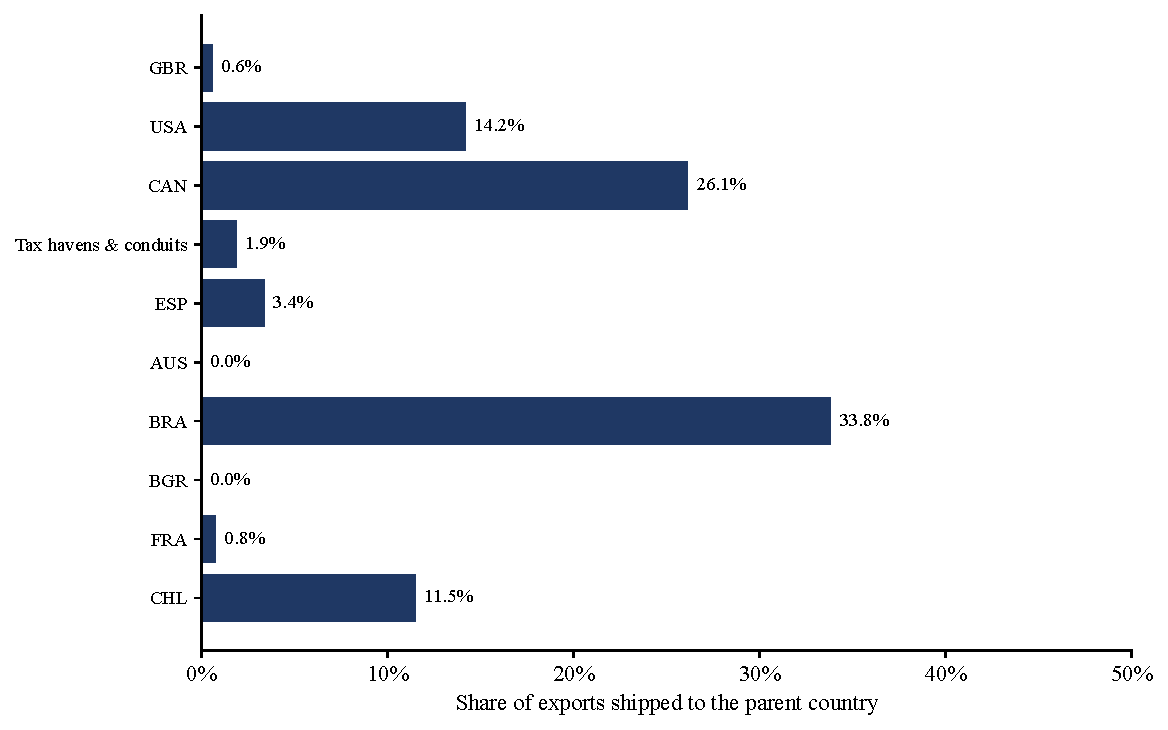
\includegraphics[width=0.85\textwidth,height=0.8\textheight,keepaspectratio]{figures/mining/fig_wp1d_home_share_by_parent_consolidated.pdf}%
  \caption{Mining and Fuels: Share of Foreign-Multinational Exports Shipped to the Parent Jurisdiction, Consolidated Parents}%
  \label{fig:homec_mining}%
  \par\vspace{2pt}%
  \parbox{0.92\textwidth}{\footnotesize %
  \textit{Notes:} Percent of each parent's exports shipped to its own jurisdiction. Dependencies are assigned to their sovereign state and tax havens and conduit jurisdictions are pooled.\\[3pt]%
  \textit{Source:} Authors' calculations based on customs data matched to Orbis and Dun \& Bradstreet.}%
  \end{figure}
% ---- Table: Mining and Fuels: Share of Foreign-Multinational Exports Shipped to the Parent Jurisdiction, Consolidated Parents
\begin{table}[H]\centering\small%
  \caption{Mining and Fuels: Share of Foreign-Multinational Exports Shipped to the Parent Jurisdiction, Consolidated Parents}%
  \label{tab:homec_t_mining}%
  \adjustbox{max width=\textwidth, max totalheight=0.8\textheight}{\begin{tabular}{lrr}
\toprule
Consolidated parent & Home share (\%) & Exports (US\$bn/yr) \\
\midrule
GBR & 0.6 & 12.2 \\
USA & 14.2 & 7.3 \\
CAN & 26.1 & 5.7 \\
Tax havens \& conduits & 1.9 & 3.3 \\
ESP & 3.4 & 1.4 \\
AUS & 0.0 & 0.9 \\
BRA & 33.8 & 0.7 \\
BGR & 0.0 & 0.5 \\
FRA & 0.8 & 0.5 \\
CHL & 11.5 & 0.4 \\
\bottomrule
\end{tabular}
}%
  \par\vspace{3pt}%
  \begin{minipage}{0.95\textwidth}\footnotesize %
  \textit{Notes:} Home share: percent of the parent's exports shipped to its own jurisdiction. Values are annual averages in US\$ billion.\\[3pt]%
  \textit{Source:} Authors' calculations based on customs data matched to Orbis and Dun \& Bradstreet.%
  \end{minipage}%
  \end{table}
% ---- Figure: Mining and Fuels: Share of Foreign-Multinational Exports Shipped to the Parent Jurisdiction
\begin{figure}[H]\centering%
  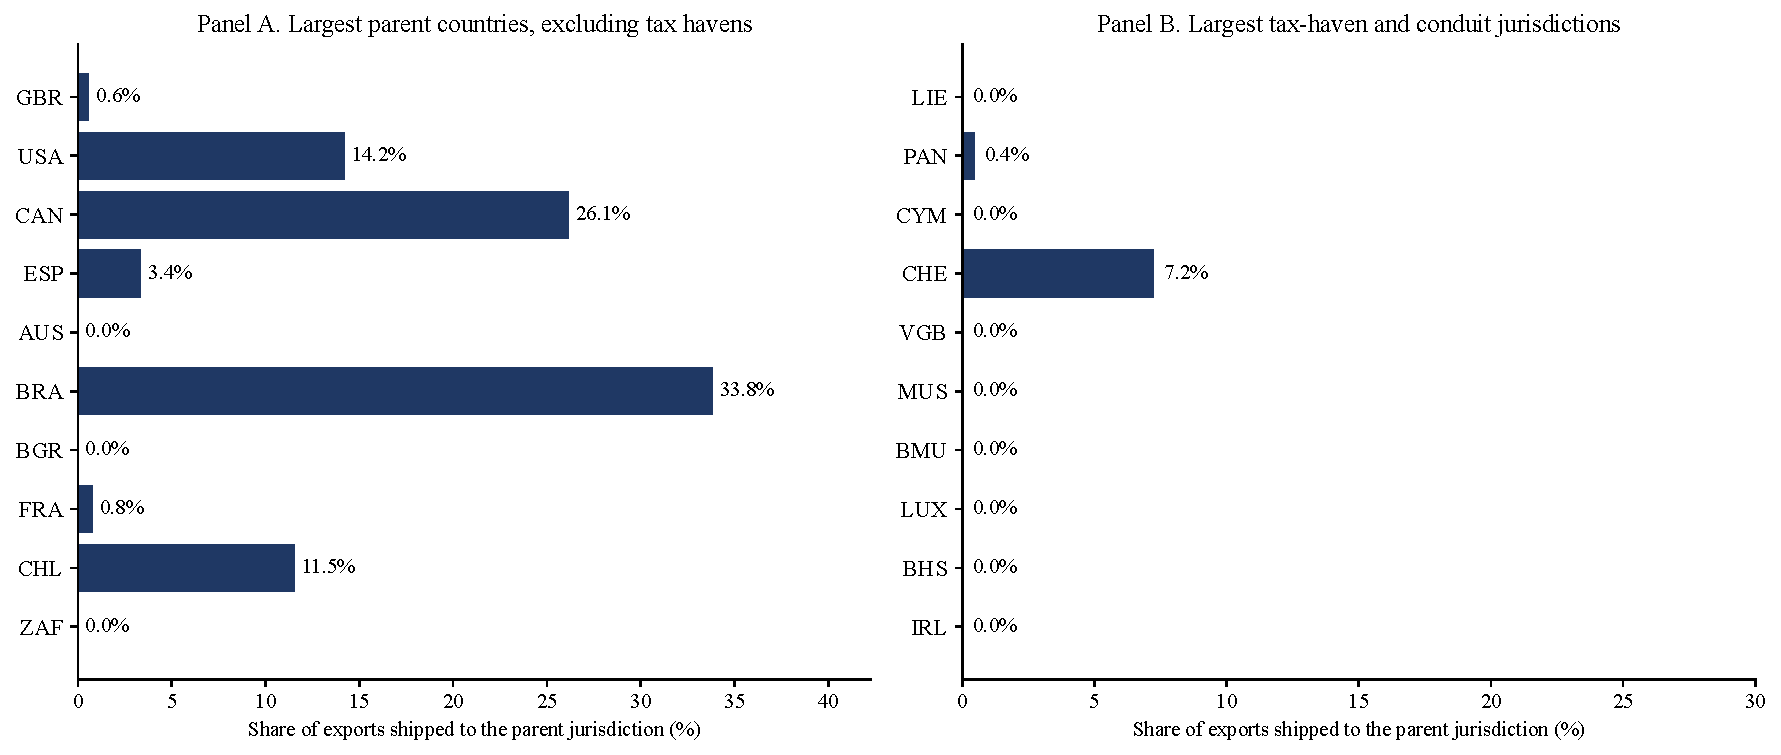
\includegraphics[width=1.0\textwidth,height=0.8\textheight,keepaspectratio]{figures/mining/fig_wp1d_home_share_haven_panels.pdf}%
  \caption{Mining and Fuels: Share of Foreign-Multinational Exports Shipped to the Parent Jurisdiction}%
  \label{fig:homeh_mining}%
  \par\vspace{2pt}%
  \parbox{0.92\textwidth}{\footnotesize %
  \textit{Notes:} Percent of each parent jurisdiction's exports shipped to that same jurisdiction. Panel A: largest parent countries, excluding tax havens; dependencies are assigned to their sovereign state. Panel B: largest tax-haven and conduit jurisdictions.\\[3pt]%
  \textit{Source:} Authors' calculations based on customs data matched to Orbis and Dun \& Bradstreet.}%
  \end{figure}
% ---- Table: Mining and Fuels: Share of Foreign-Multinational Exports Shipped to the Parent Jurisdiction
\begin{table}[H]\centering\small%
  \caption{Mining and Fuels: Share of Foreign-Multinational Exports Shipped to the Parent Jurisdiction}%
  \label{tab:homeh_t_mining}%
  \adjustbox{max width=\textwidth, max totalheight=0.8\textheight}{\begin{tabular}{llrr}
\toprule
Panel & Parent & Home share (\%) & Exports (US\$bn/yr) \\
\midrule
Panel A & GBR & 0.6 & 11.9 \\
Panel A & USA & 14.2 & 7.3 \\
Panel A & CAN & 26.1 & 5.7 \\
Panel A & ESP & 3.4 & 1.4 \\
Panel A & AUS & 0.0 & 0.9 \\
Panel A & BRA & 33.8 & 0.7 \\
Panel A & BGR & 0.0 & 0.5 \\
Panel A & FRA & 0.8 & 0.5 \\
Panel A & CHL & 11.5 & 0.4 \\
Panel A & ZAF & 0.0 & 0.3 \\
\midrule
Panel B & LIE & 0.0 & 2.0 \\
Panel B & PAN & 0.4 & 1.0 \\
Panel B & CYM & 0.0 & 0.2 \\
Panel B & CHE & 7.2 & 0.1 \\
Panel B & VGB & 0.0 & 0.1 \\
Panel B & MUS & 0.0 & 0.1 \\
Panel B & BMU & 0.0 & 0.1 \\
Panel B & LUX & 0.0 & 0.0 \\
Panel B & BHS & 0.0 & 0.0 \\
Panel B & IRL & 0.0 & 0.0 \\
\bottomrule
\end{tabular}
}%
  \par\vspace{3pt}%
  \begin{minipage}{0.95\textwidth}\footnotesize %
  \textit{Notes:} Home share: percent of the parent's exports shipped to its own jurisdiction. Panel A: largest parent countries, excluding tax havens. Panel B: largest tax-haven and conduit jurisdictions. Values are annual averages in US\$ billion.\\[3pt]%
  \textit{Source:} Authors' calculations based on customs data matched to Orbis and Dun \& Bradstreet.%
  \end{minipage}%
  \end{table}

\subsection{Destination Markets}
% ---- Figure: Mining and Fuels: Exports to the United States, by Type of Exporter and Exporting Country
\begin{figure}[H]\centering%
  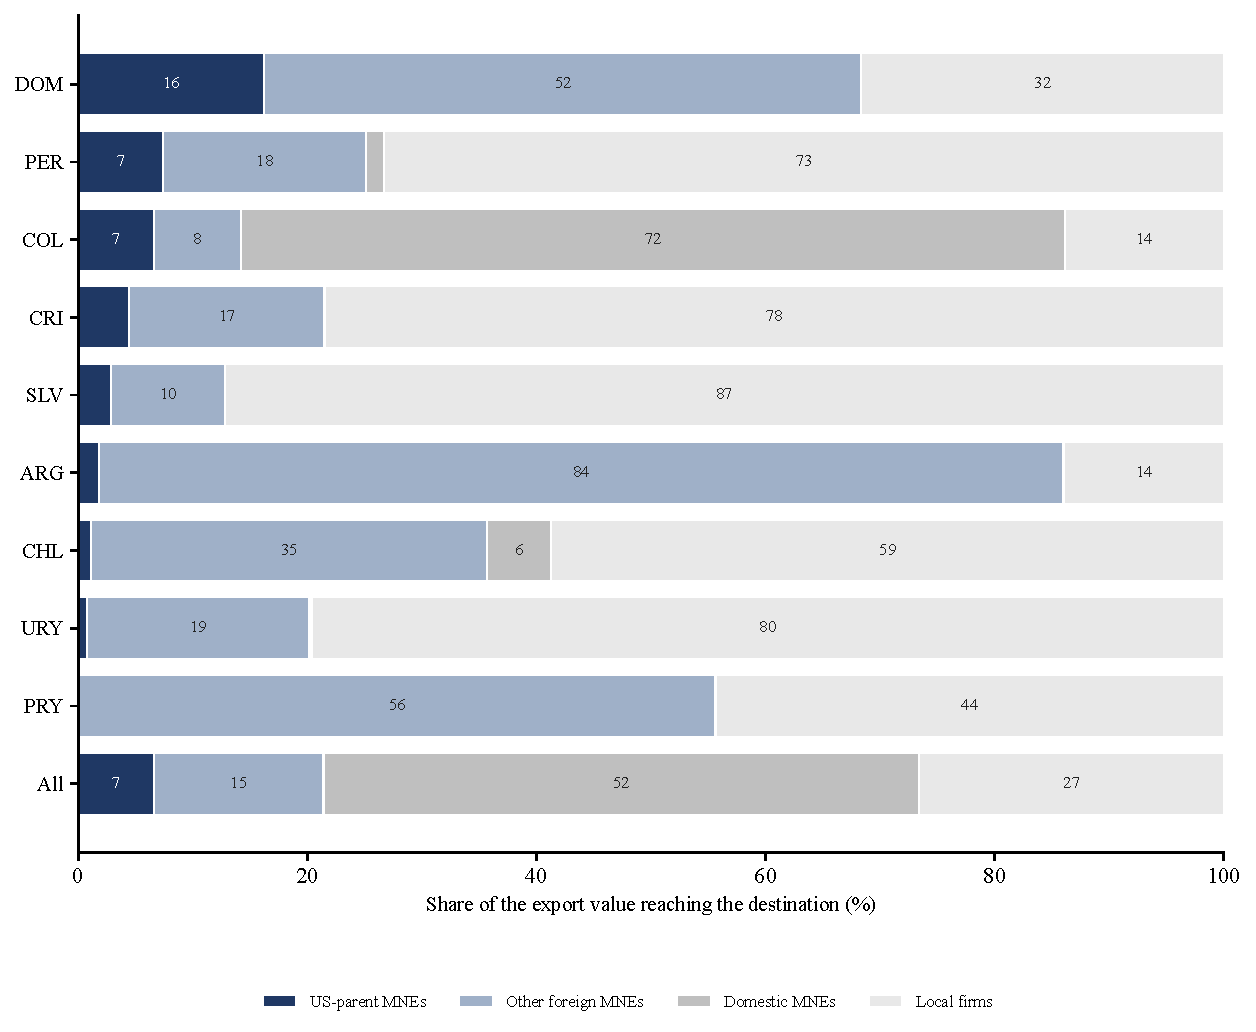
\includegraphics[width=0.9\textwidth,height=0.8\textheight,keepaspectratio]{figures/mining/fig_wp3_to_usa_carriers.pdf}%
  \caption{Mining and Fuels: Exports to the United States, by Type of Exporter and Exporting Country}%
  \label{fig:to_usa_f_mining}%
  \par\vspace{2pt}%
  \parbox{0.92\textwidth}{\footnotesize %
  \textit{Notes:} Percent of each country's mining and fuels exports to the United States, by type of exporter.\\[3pt]%
  \textit{Source:} Authors' calculations based on customs data matched to Orbis and Dun \& Bradstreet.}%
  \end{figure}
% ---- Table: Mining and Fuels: Exports to the United States, by Type of Exporter and Exporting Country
\begin{table}[H]\centering\small%
  \caption{Mining and Fuels: Exports to the United States, by Type of Exporter and Exporting Country}%
  \label{tab:to_usa_mining}%
  \adjustbox{max width=\textwidth, max totalheight=0.8\textheight}{\begin{tabular}{lrrrrr}
\toprule
Origin & Exports to the USA (US\$bn/yr) & US-parent MNEs (\%) & Other foreign MNEs (\%) & Domestic MNEs (\%) & Local firms (\%) \\
\midrule
DOM & 0.5 & 16.2 & 52.1 & 0.0 & 31.6 \\
PER & 3.0 & 7.4 & 17.7 & 1.6 & 73.3 \\
COL & 9.9 & 6.6 & 7.6 & 71.9 & 13.9 \\
CRI & 0.1 & 4.4 & 17.1 & 0.0 & 78.4 \\
SLV & 0.0 & 2.9 & 9.9 & 0.0 & 87.2 \\
ARG & 0.9 & 1.8 & 84.2 & 0.1 & 13.9 \\
CHL & 0.3 & 1.1 & 34.6 & 5.6 & 58.7 \\
URY & 0.0 & 0.8 & 19.4 & 0.2 & 79.6 \\
PRY & 0.0 & 0.0 & 55.6 & 0.0 & 44.3 \\
\midrule
All & 14.6 & 6.6 & 14.8 & 52.0 & 26.6 \\
\bottomrule
\end{tabular}
}%
  \par\vspace{3pt}%
  \begin{minipage}{0.95\textwidth}\footnotesize %
  \textit{Notes:} Percent of each country's mining and fuels exports to the United States, by type of exporter. Values are annual averages in US\$ billion.\\[3pt]%
  \textit{Source:} Authors' calculations based on customs data matched to Orbis and Dun \& Bradstreet.%
  \end{minipage}%
  \end{table}
% ---- Figure: Mining and Fuels: Ownership of Exports to the Main Destination Markets
\begin{figure}[H]\centering%
  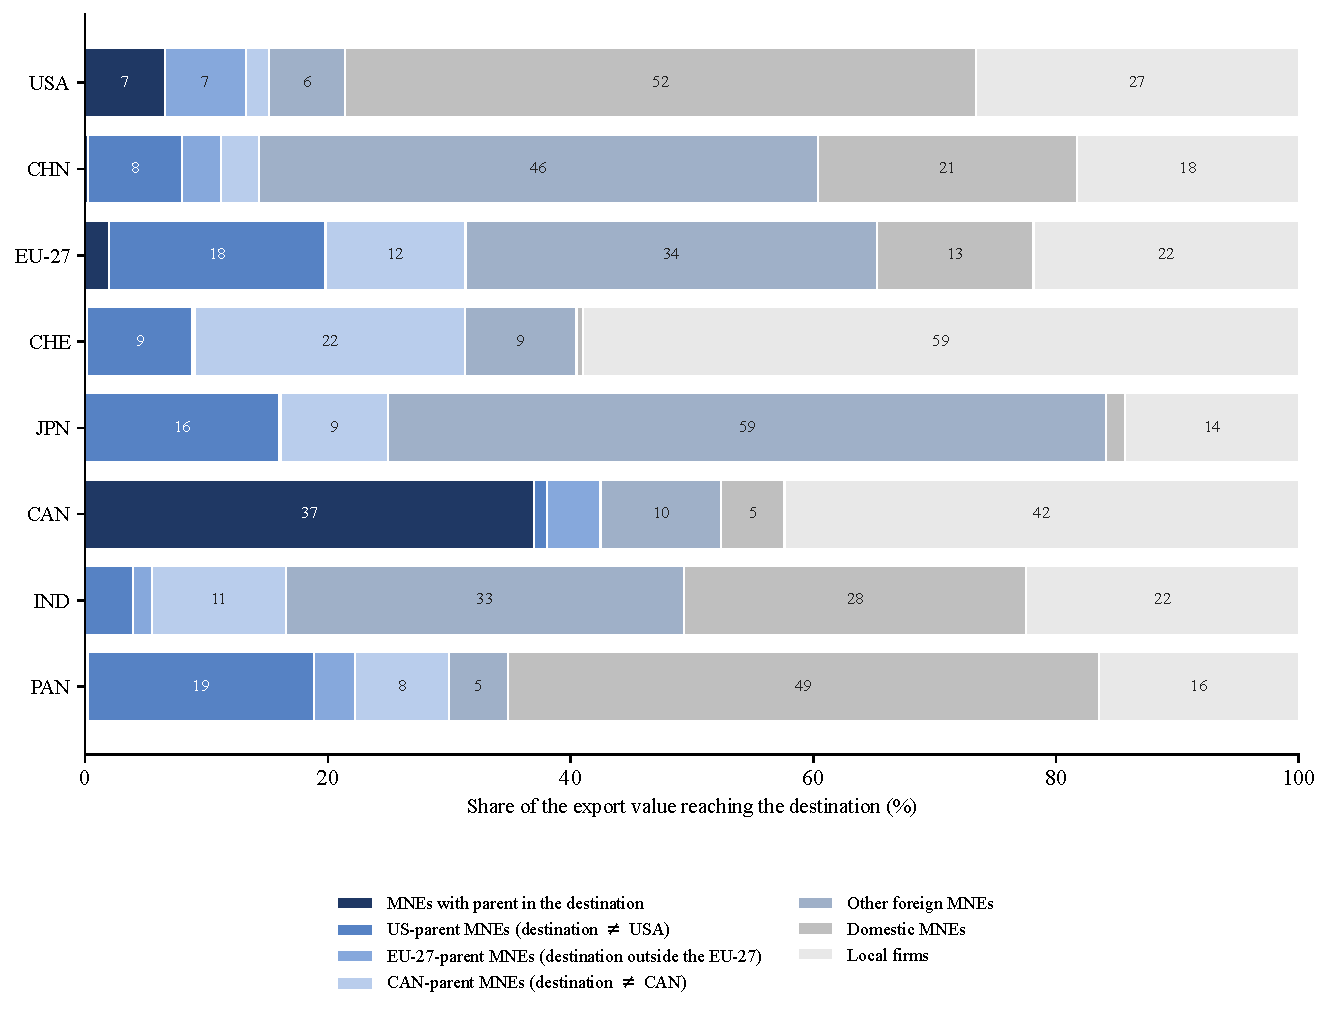
\includegraphics[width=0.95\textwidth,height=0.8\textheight,keepaspectratio]{figures/mining/fig_wp3_dest_carriers.pdf}%
  \caption{Mining and Fuels: Ownership of Exports to the Main Destination Markets}%
  \label{fig:dest_f_mining}%
  \par\vspace{2pt}%
  \parbox{0.92\textwidth}{\footnotesize %
  \textit{Notes:} Percent of the export value reaching each destination, by type of exporter. The first segment is exports by MNEs whose parent is located in that destination. EU-27 member states are pooled.\\[3pt]%
  \textit{Source:} Authors' calculations based on customs data matched to Orbis and Dun \& Bradstreet.}%
  \end{figure}
% ---- Table: Mining and Fuels: Ownership of Exports to the Main Destination Markets
\begin{table}[H]\centering\footnotesize%
  \caption{Mining and Fuels: Ownership of Exports to the Main Destination Markets}%
  \label{tab:dest_mining}%
  \adjustbox{max width=\textwidth, max totalheight=0.8\textheight}{\begin{tabular}{lrrrrrrrr}
\toprule
Destination & \multicolumn{1}{p{1.5cm}}{\raggedright Exports (US\$bn/yr)} & \multicolumn{1}{p{2.2cm}}{\raggedright MNEs with parent in the destination (\%)} & \multicolumn{1}{p{1.6cm}}{\raggedright US-parent MNEs (\%)} & \multicolumn{1}{p{1.6cm}}{\raggedright EU-27-parent MNEs (\%)} & \multicolumn{1}{p{1.6cm}}{\raggedright CAN-parent MNEs (\%)} & \multicolumn{1}{p{1.6cm}}{\raggedright Other foreign MNEs (\%)} & \multicolumn{1}{p{1.6cm}}{\raggedright Domestic MNEs (\%)} & \multicolumn{1}{p{1.5cm}}{\raggedright Local firms (\%)} \\
\midrule
USA & 14.6 & 6.6 & -- & 6.7 & 1.9 & 6.2 & 52.0 & 26.6 \\
CHN & 13.8 & 0.3 & 7.7 & 3.2 & 3.1 & 46.0 & 21.3 & 18.3 \\
EU-27 & 8.5 & 2.0 & 17.8 & -- & 11.5 & 33.9 & 12.9 & 21.9 \\
CHE & 4.9 & 0.2 & 8.7 & 0.2 & 22.2 & 9.2 & 0.5 & 59.0 \\
JPN & 3.8 & 0.0 & 16.0 & 0.1 & 8.8 & 59.2 & 1.6 & 14.3 \\
CAN & 4.4 & 37.0 & 1.1 & 4.4 & -- & 9.9 & 5.2 & 42.4 \\
IND & 3.2 & 0.0 & 3.9 & 1.5 & 11.0 & 32.8 & 28.2 & 22.4 \\
PAN & 2.5 & 0.2 & 18.7 & 3.4 & 7.8 & 4.8 & 48.7 & 16.5 \\
\bottomrule
\end{tabular}
}%
  \par\vspace{3pt}%
  \begin{minipage}{0.95\textwidth}\footnotesize %
  \textit{Notes:} Percent of the export value reaching each destination, by type of exporter. EU-27 member states are pooled. Values are annual averages in US\$ billion.\\[3pt]%
  \textit{Source:} Authors' calculations based on customs data matched to Orbis and Dun \& Bradstreet.%
  \end{minipage}%
  \end{table}
% ---- Table: Mining and Fuels: Main Products Shipped by US-Parent Multinationals to the United States
\begin{table}[H]\centering\footnotesize%
  \caption{Mining and Fuels: Main Products Shipped by US-Parent Multinationals to the United States}%
  \label{tab:us_home_mining}%
  \adjustbox{max width=\textwidth, max totalheight=0.8\textheight}{\begin{tabular}{llrrrrrl}
\toprule
HS6 & Description & \multicolumn{1}{p{1.7cm}}{\raggedright US-parent exports to the USA (US\$bn/yr)} & \multicolumn{1}{p{1.7cm}}{\raggedright \% of all US-parent exports to the USA} & \multicolumn{1}{p{2.0cm}}{\raggedright \% of US-parent exports of the product going to the USA} & \multicolumn{1}{p{1.9cm}}{\raggedright All exports of the product to the USA (US\$bn/yr)} & \multicolumn{1}{p{2.2cm}}{\raggedright US-parent share of exports of the product to the USA (\%)} & \multicolumn{1}{p{2.6cm}}{\raggedright Main origins of the US-parent shipments (\% of the line)} \\
\midrule
270900 & Petroleum oils \& oils obt. from bituminous mi... & 0.41 & 48.7 & 24 & 7.84 & 5 & COL 100\%, ARG 0\% \\
270112 & Bituminous coal, whether/not pulverised but n... & 0.19 & 22.6 & 9 & 0.39 & 48 & COL 100\% \\
261390 & Molybdenum ores \& concentrates, other than ro... & 0.15 & 14.8 & 99 & 0.18 & 79 & PER 100\% \\
711319 & Articles of jewellery \& parts thereof , of ot... & 0.06 & 4.9 & 100 & 0.35 & 17 & DOM 100\% \\
710812 & Gold (incl. gold plated with platinum), in un... & 0.02 & 1.7 & 4 & 2.72 & 1 & PER 56\%, COL 23\%, CHL 21\% \\
271012 & Light petroleum oils and preparations [HS2012... & 0.01 & 1.6 & 40 & 0.27 & 5 & COL 100\%, CRI 0\%, ARG 0\% \\
270750 & Aromatic hydrocarbon mixtures of which 65\%/mo... & 0.02 & 1.4 & 98 & 0.02 & 97 & ARG 100\%, COL 0\% \\
271011 & Light petroleum oils \& preparations & 0.01 & 1.2 & 42 & 0.69 & 4 & COL 100\%, SLV 0\%, DOM 0\% \\
271111 & Natural gas, liquefied & 0.01 & 1.0 & 1 & 0.01 & 100 & PER 100\%, DOM 0\% \\
711311 & Articles of jewellery \& parts thereof , of si... & 0.01 & 0.7 & 100 & 0.06 & 14 & DOM 100\%, ARG 0\%, PER 0\% \\
711291 & Waste \& scrap of gold, incl. metal clad with ... & 0.01 & 0.5 & 100 & 0.06 & 7 & DOM 72\%, CRI 20\%, COL 5\% \\
710813 & Gold (incl. gold plated with platinum), non-m... & 0.01 & 0.5 & 100 & 0.12 & 5 & DOM 99\%, CRI 1\% \\
271019 & Petroleum oils \& oils obtained from bituminou... & 0.00 & 0.2 & 2 & 1.14 & 0 & SLV 91\%, COL 5\%, URY 3\% \\
711299 & Waste \& scrap of precious metal/of metal clad... & 0.00 & 0.1 & 83 & 0.01 & 22 & CRI 92\%, COL 3\%, DOM 3\% \\
711230 & Ash containing precious metal/precious metal ... & 0.00 & 0.1 & 100 & 0.00 & 20 & DOM 100\% \\
\midrule
All lines & & 0.9 & 100.0 & 12 & 14.6 & 7 & \\
\bottomrule
\end{tabular}
}%
  \par\vspace{3pt}%
  \begin{minipage}{0.95\textwidth}\footnotesize %
  \textit{Notes:} Fifteen HS6 products with the largest exports by US-parent MNEs to the United States. Values are annual averages in US\$ billion.\\[3pt]%
  \textit{Source:} Authors' calculations based on customs data matched to Orbis and Dun \& Bradstreet.%
  \end{minipage}%
  \end{table}
% ---- Figure: Mining and Fuels: US-Parent Share of Exports to the United States, Main Products Shipped by US-Parent Multinationals
\begin{figure}[H]\centering%
  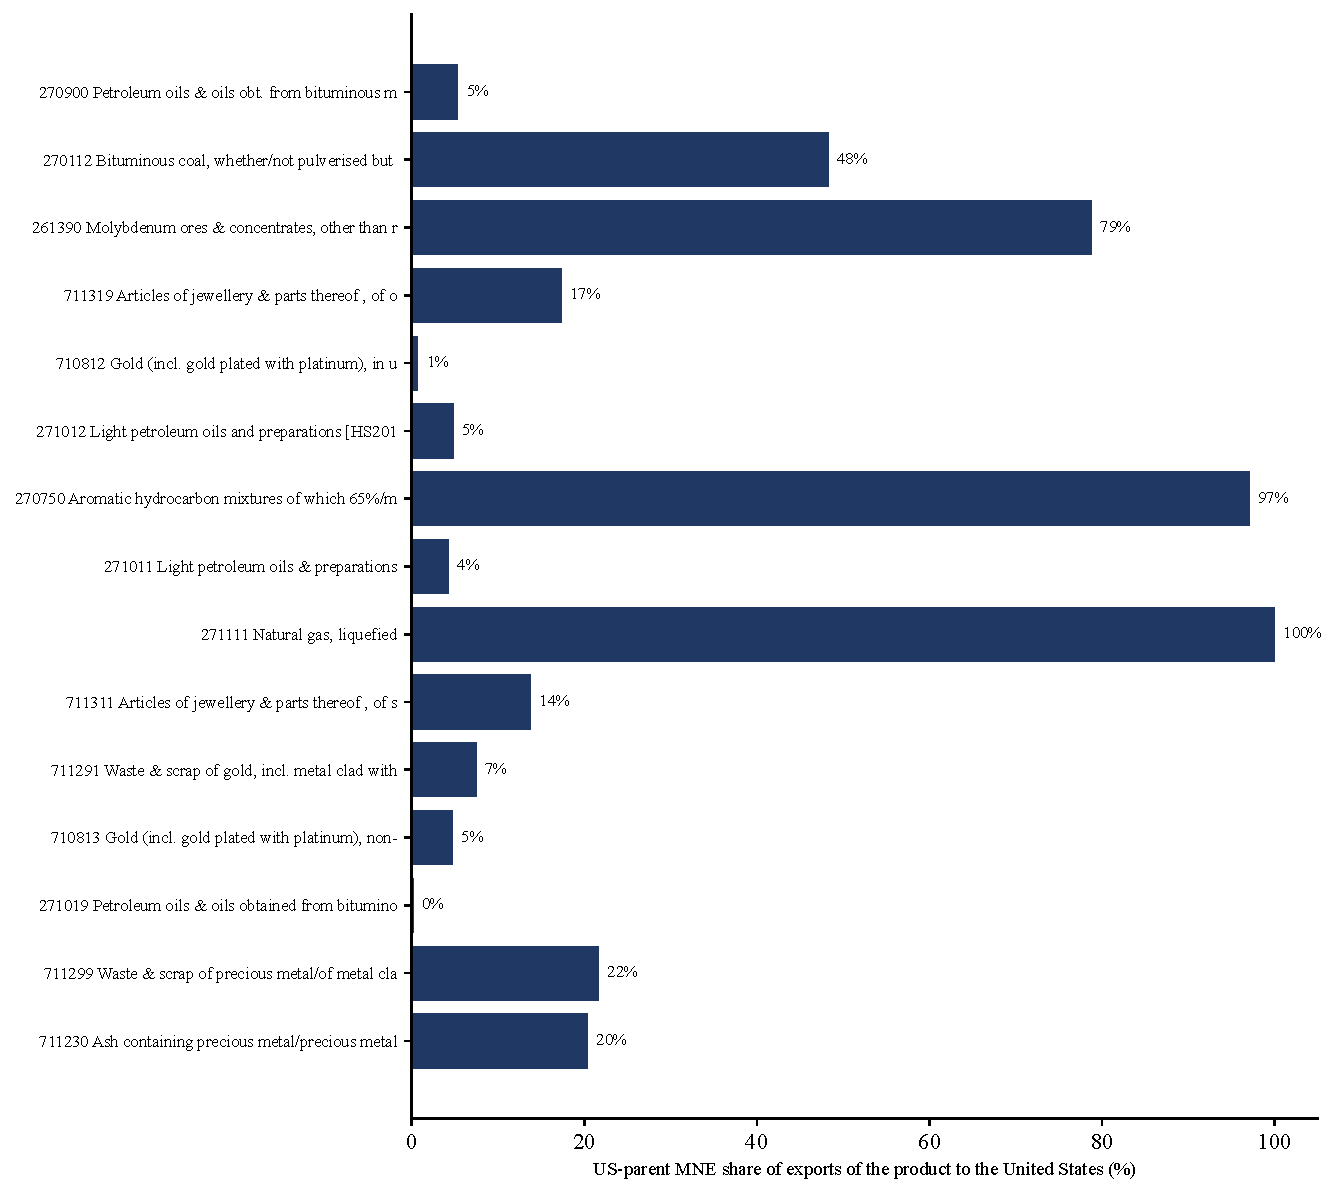
\includegraphics[width=0.95\textwidth,height=0.8\textheight,keepaspectratio]{figures/mining/fig_wp3_us_home_products.pdf}%
  \caption{Mining and Fuels: US-Parent Share of Exports to the United States, Main Products Shipped by US-Parent Multinationals}%
  \label{fig:us_home_f_mining}%
  \par\vspace{2pt}%
  \parbox{0.92\textwidth}{\footnotesize %
  \textit{Notes:} Percent of the nine countries' exports of each product to the United States shipped by US-parent MNEs; the fifteen products with the largest US-parent exports to the United States.\\[3pt]%
  \textit{Source:} Authors' calculations based on customs data matched to Orbis and Dun \& Bradstreet.}%
  \end{figure}
% ---- Table: Mining and Fuels: Largest Export Products to the United States, by Type of Exporter
\begin{table}[H]\centering\footnotesize%
  \caption{Mining and Fuels: Largest Export Products to the United States, by Type of Exporter}%
  \label{tab:to_usa_prod_mining}%
  \adjustbox{max width=\textwidth, max totalheight=0.8\textheight}{\begin{tabular}{llrrrrr}
\toprule
HS6 & Description & \multicolumn{1}{p{2.0cm}}{\raggedright Exports to the USA (US\$bn/yr)} & \multicolumn{1}{p{1.8cm}}{\raggedright US-parent MNEs (\%)} & \multicolumn{1}{p{1.8cm}}{\raggedright Other foreign MNEs (\%)} & \multicolumn{1}{p{1.8cm}}{\raggedright Domestic MNEs (\%)} & \multicolumn{1}{p{1.8cm}}{\raggedright Local firms (\%)} \\
\midrule
270900 & Petroleum oils \& oils obt. from bituminous mi... & 7.84 & 5 & 10 & 81 & 4 \\
710812 & Gold (incl. gold plated with platinum), in un... & 2.72 & 1 & 16 & 9 & 74 \\
271019 & Petroleum oils \& oils obtained from bituminou... & 1.14 & 0 & 14 & 51 & 35 \\
271011 & Light petroleum oils \& preparations & 0.69 & 4 & 14 & 5 & 76 \\
270112 & Bituminous coal, whether/not pulverised but n... & 0.39 & 48 & 32 & 1 & 19 \\
710691 & Silver (incl. silver plated with gold/platinu... & 0.34 & 0 & 31 & 0 & 69 \\
271012 & Light petroleum oils and preparations [HS2012... & 0.27 & 5 & 32 & 43 & 20 \\
711319 & Articles of jewellery \& parts thereof , of ot... & 0.35 & 17 & 46 & 0 & 37 \\
261390 & Molybdenum ores \& concentrates, other than ro... & 0.18 & 79 & 18 & 0 & 3 \\
710813 & Gold (incl. gold plated with platinum), non-m... & 0.12 & 5 & 51 & 3 & 41 \\
251010 & Natural calcium phosphates, natural aluminium... & 0.11 & 0 & 100 & 0 & 0 \\
250100 & Salt (incl. table salt \& denatured salt) \& pu... & 0.06 & 0 & 62 & 9 & 28 \\
710391 & Rubies, sapphires \& emeralds, worked othw. th... & 0.06 & 0 & 28 & 0 & 72 \\
711291 & Waste \& scrap of gold, incl. metal clad with ... & 0.06 & 7 & 5 & 0 & 87 \\
711311 & Articles of jewellery \& parts thereof , of si... & 0.06 & 14 & 57 & 0 & 29 \\
\bottomrule
\end{tabular}
}%
  \par\vspace{3pt}%
  \begin{minipage}{0.95\textwidth}\footnotesize %
  \textit{Notes:} Fifteen largest HS6 products exported to the United States; percent of each product's exports to the United States by type of exporter. Values are annual averages in US\$ billion.\\[3pt]%
  \textit{Source:} Authors' calculations based on customs data matched to Orbis and Dun \& Bradstreet.%
  \end{minipage}%
  \end{table}

\section{Fact 4: A Small Set of Large Multinational Groups Accounts for Most Exports}\label{sec:f4s_mining}

\subsection{Size of the Group's Global Network}
% ---- Figure: Mining and Fuels: Foreign-Multinational Exports and Number of Parents, by Size of the Group's Global Network
\begin{figure}[H]\centering%
  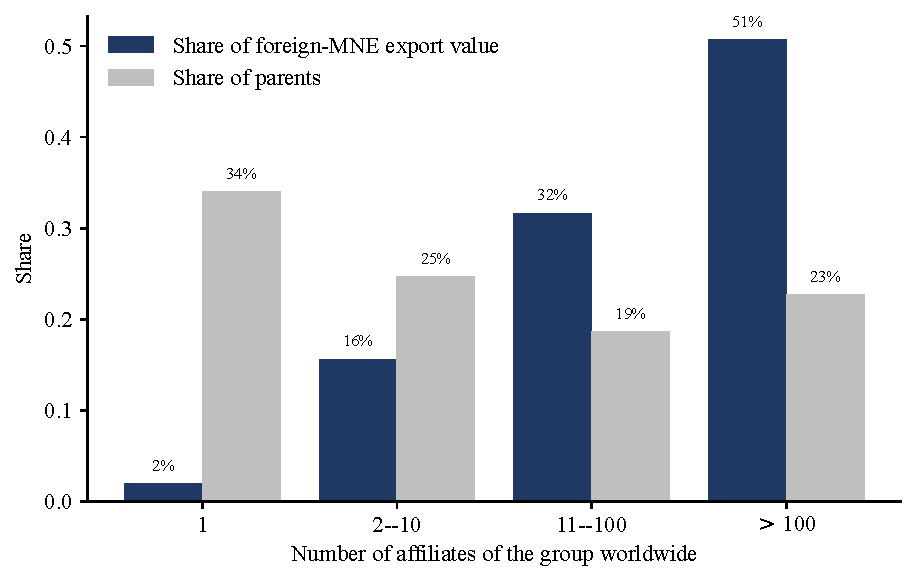
\includegraphics[width=0.7\textwidth,height=0.8\textheight,keepaspectratio]{figures/mining/fig_wp0_fig5_network.pdf}%
  \caption{Mining and Fuels: Foreign-Multinational Exports and Number of Parents, by Size of the Group's Global Network}%
  \label{fig:net_mining}%
  \par\vspace{2pt}%
  \parbox{0.92\textwidth}{\footnotesize %
  \textit{Notes:} Shares of foreign-MNE mining and fuels export value and of parents, by the number of affiliates the group has worldwide.\\[3pt]%
  \textit{Source:} Authors' calculations based on customs data matched to Orbis and Dun \& Bradstreet.}%
  \end{figure}
% ---- Table: Mining and Fuels: Foreign-Multinational Exports and Number of Parents, by Size of the Group's Global Network
\begin{table}[H]\centering\small%
  \caption{Mining and Fuels: Foreign-Multinational Exports and Number of Parents, by Size of the Group's Global Network}%
  \label{tab:net_t_mining}%
  \adjustbox{max width=\textwidth, max totalheight=0.8\textheight}{\begin{tabular}{lrrr}
\toprule
Affiliates worldwide & Parents & Share of parents (\%) & Share of foreign-MNE export value (\%) \\
\midrule
1 & 521 & 34.0 & 2.0 \\
2--10 & 378 & 24.7 & 15.6 \\
11--100 & 285 & 18.6 & 31.7 \\
$>$100 & 348 & 22.7 & 50.7 \\
\midrule
All parents & 1,532 & 100 & 100 \\
\bottomrule
\end{tabular}
}%
  \par\vspace{3pt}%
  \begin{minipage}{0.95\textwidth}\footnotesize %
  \textit{Notes:} Number and share of parents, and share of foreign-MNE mining and fuels export value, by the number of affiliates the group has worldwide.\\[3pt]%
  \textit{Source:} Authors' calculations based on customs data matched to Orbis and Dun \& Bradstreet.%
  \end{minipage}%
  \end{table}

\subsection{Concentration within Products}
% ---- Figure: Mining and Fuels: Export Concentration within Products: Firms and Groups
\begin{figure}[H]\centering%
  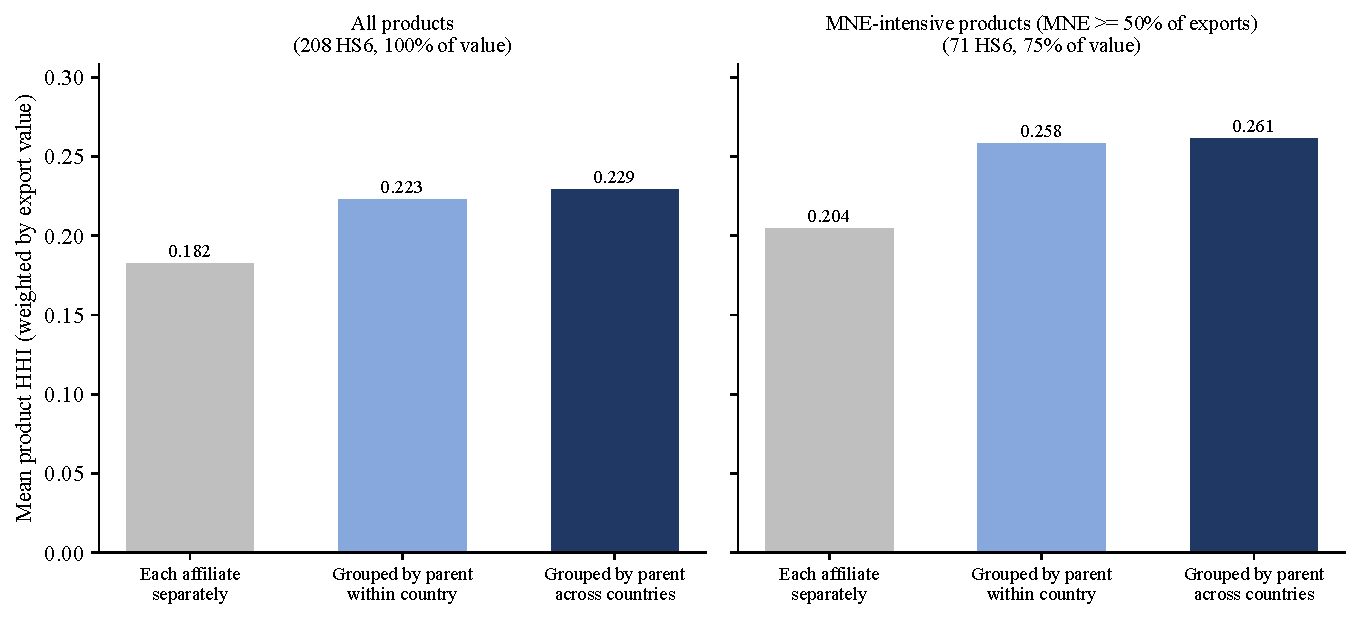
\includegraphics[width=0.9\textwidth,height=0.8\textheight,keepaspectratio]{figures/mining/fig_wp0_fig6_hhi.pdf}%
  \caption{Mining and Fuels: Export Concentration within Products: Firms and Groups}%
  \label{fig:hhi_mining}%
  \par\vspace{2pt}%
  \parbox{0.92\textwidth}{\footnotesize %
  \textit{Notes:} Mean Herfindahl index of exporters within each HS6 product, weighted by export value, counting each affiliate separately or grouping affiliates by parent within or across countries. Right panel: products where MNEs account for at least half of exports.\\[3pt]%
  \textit{Source:} Authors' calculations based on customs data matched to Orbis and Dun \& Bradstreet.}%
  \end{figure}
% ---- Table: Mining and Fuels: Export Concentration within Products: Firms and Groups
\begin{table}[H]\centering\small%
  \caption{Mining and Fuels: Export Concentration within Products: Firms and Groups}%
  \label{tab:hhi_t_mining}%
  \adjustbox{max width=\textwidth, max totalheight=0.8\textheight}{\begin{tabular}{llrrr}
\toprule
Sample & Measure & Firm level & Groups within country & Groups across countries \\
\midrule
\multicolumn{5}{l}{\textit{All products: 208 HS6, 100\% of value}} \\
 & Mean HHI & 0.182 & 0.223 & 0.229 \\
 & Mean top-exporter share & 31.1\% & 34.9\% & 36.7\% \\
 & Effective number of exporters (1/HHI) & 11.4 & 10.6 & 7.9 \\
\multicolumn{5}{l}{\textit{MNE-intensive products (MNE $\geq$ 50\% of exports): 71 HS6, 75\% of value}} \\
 & Mean HHI & 0.204 & 0.258 & 0.261 \\
 & Mean top-exporter share & 34.6\% & 39.7\% & 39.7\% \\
 & Effective number of exporters (1/HHI) & 7.7 & 6.7 & 6.3 \\
\bottomrule
\end{tabular}
}%
  \par\vspace{3pt}%
  \begin{minipage}{0.95\textwidth}\footnotesize %
  \textit{Notes:} Means across HS6 products, weighted by export value. Firm level: each affiliate counted separately. Groups: affiliates grouped by ultimate parent within each exporting country or across countries.\\[3pt]%
  \textit{Source:} Authors' calculations based on customs data matched to Orbis and Dun \& Bradstreet.%
  \end{minipage}%
  \end{table}

\subsection{Groups and Affiliates}
% ---- Table: Mining and Fuels: Multinational Affiliates and Groups in Origin--Destination--Product--Year Cells
\begin{table}[H]\centering\small%
  \caption{Mining and Fuels: Multinational Affiliates and Groups in Origin--Destination--Product--Year Cells}%
  \label{tab:grp_mining}%
  \adjustbox{max width=\textwidth, max totalheight=0.8\textheight}{\begin{tabular}{lr}
\toprule
Origin-destination-product-year cells with $\geq 1$ MNE & \\
\midrule
Cells & 17,619 \\
MNE affiliates per cell (mean) & 1.69 \\
MNE groups per cell (mean) & 1.67 \\
Affiliates per group, pooled & 1.01 \\
Affiliates per group, mean weighted by export value & 1.09 \\
Cells where one group exports through $>1$ affiliate (\%) & 1.5 \\
\bottomrule
\end{tabular}
}%
  \par\vspace{3pt}%
  \begin{minipage}{0.95\textwidth}\footnotesize %
  \textit{Notes:} Cells with at least one MNE. Group: ultimate parent in Orbis or Dun \& Bradstreet (parent name when the identifier is missing).\\[3pt]%
  \textit{Source:} Authors' calculations based on customs data matched to Orbis and Dun \& Bradstreet.%
  \end{minipage}%
  \end{table}
% ---- Table: Mining and Fuels: Multinational Presence and Exports: Affiliates and Groups
\begin{table}[H]\centering\small%
  \caption{Mining and Fuels: Multinational Presence and Exports: Affiliates and Groups}%
  \label{tab:grp_r_mining}%
  \adjustbox{max width=\textwidth, max totalheight=0.8\textheight}{\begin{tabular}{lcccccc} \hline
 & \multicolumn{3}{c}{Origin $\times$ year, destination $\times$ year, product FE} & \multicolumn{3}{c}{Origin $\times$ dest. $\times$ product, origin $\times$ dest. $\times$ year FE} \\
 & (1) & (2) & (3) & (4) & (5) & (6) \\ \hline
\multicolumn{7}{l}{\textit{Panel A. Dependent variable: $\ln$ exports, all firms}} \\
$\ln$(\# MNE firms) & 2.5367*** &  &  & 0.8789*** &  &  \\
 & (0.0797) &  &  & (0.0732) &  &  \\
$\ln$(\# MNE groups) &  & 2.5655*** & 2.5498*** &  & 0.8787*** & 0.8799*** \\
 &  & (0.0800) & (0.0794) &  & (0.0735) & (0.0734) \\
$\ln$(affiliates per group) &  &  & 1.7853*** &  &  & 0.8051*** \\
 &  &  & (0.5380) &  &  & (0.2947) \\
\midrule
\multicolumn{7}{l}{\textit{Panel B. Dependent variable: $\ln$ exports, non-MNE firms}} \\
$\ln$(\# MNE firms) & 1.4518*** &  &  & 0.1605* &  &  \\
 & (0.0976) &  &  & (0.0952) &  &  \\
$\ln$(\# MNE groups) &  & 1.4559*** & 1.4511*** &  & 0.1684* & 0.1651* \\
 &  & (0.0974) & (0.0970) &  & (0.0939) & (0.0947) \\
$\ln$(affiliates per group) &  &  & 1.5168** &  &  & -0.5378 \\
 &  &  & (0.7448) &  &  & (0.7197) \\
\hline
Product FE & $\checkmark$ & $\checkmark$ & $\checkmark$ &  &  &  \\
Origin $\times$ year FE & $\checkmark$ & $\checkmark$ & $\checkmark$ &  &  &  \\
Destination $\times$ year FE & $\checkmark$ & $\checkmark$ & $\checkmark$ &  &  &  \\
Origin $\times$ dest.\ $\times$ product FE &  &  &  & $\checkmark$ & $\checkmark$ & $\checkmark$ \\
Origin $\times$ dest.\ $\times$ year FE &  &  &  & $\checkmark$ & $\checkmark$ & $\checkmark$ \\
Observations (Panel A) & 17,183 & 17,183 & 17,183 & 13,668 & 13,668 & 13,668 \\
Observations (Panel B) & 7,153 & 7,153 & 7,153 & 5,898 & 5,898 & 5,898 \\
\hline
\end{tabular}
}%
  \par\vspace{3pt}%
  \begin{minipage}{0.95\textwidth}\footnotesize %
  \textit{Notes:} Observations are origin--destination--HS6--year cells. Mining and Fuels products only. Dependent variable: $\ln$ exports of the cell (Panel A) and of the non-MNE firms in the cell (Panel B). Regressors: $\ln$ number of MNE affiliates or $\ln$ number of MNE groups (distinct ultimate parents). Standard errors clustered by origin--destination pair in parentheses. *** $p<0.01$, ** $p<0.05$, * $p<0.1$.\\[3pt]%
  \textit{Source:} Authors' calculations based on customs data matched to Orbis and Dun \& Bradstreet.%
  \end{minipage}%
  \end{table}

\section{Fact 5: Multinational Presence Is Associated with Higher Exports}\label{sec:f5_mining}
% ---- Table: Mining and Fuels: Multinational Presence and Exports
\begin{table}[H]\centering\small%
  \caption{Mining and Fuels: Multinational Presence and Exports}%
  \label{tab:t1_mining}%
  \adjustbox{max width=\textwidth, max totalheight=0.8\textheight}{\begin{tabular}{lcccccc} \hline
 & \multicolumn{3}{c}{Intensive: $\ln$(\# MNE firms)} & \multicolumn{3}{c}{Extensive: any MNE present} \\
 & (1) & (2) & (3) & (1) & (2) & (3) \\ \hline
\multicolumn{7}{l}{\textit{Panel A. Dependent variable: $\ln$ exports, all firms}} \\
$\ln$(\# MNE firms) & 2.5346*** & 2.5367*** & 0.8789*** &  &  &  \\
 & (0.0755) & (0.0797) & (0.0732) &  &  &  \\
Any MNE present &  &  &  & 1.3777*** & 1.3943*** & 0.6626*** \\
 &  &  &  & (0.0890) & (0.0929) & (0.0589) \\
\midrule
\multicolumn{7}{l}{\textit{Panel B. Dependent variable: $\ln$ exports, non-MNE firms}} \\
$\ln$(\# MNE firms) & 1.4407*** & 1.4518*** & 0.1605* &  &  &  \\
 & (0.0898) & (0.0976) & (0.0952) &  &  &  \\
Any MNE present &  &  &  & 1.6657*** & 1.6631*** & 0.1846*** \\
 &  &  &  & (0.0962) & (0.1016) & (0.0505) \\
\hline
Origin FE & $\checkmark$ &  &  & $\checkmark$ &  &  \\
Destination FE & $\checkmark$ &  &  & $\checkmark$ &  &  \\
Product FE & $\checkmark$ & $\checkmark$ &  & $\checkmark$ & $\checkmark$ &  \\
Year FE & $\checkmark$ &  &  & $\checkmark$ &  &  \\
Origin $\times$ year FE &  & $\checkmark$ &  &  & $\checkmark$ &  \\
Destination $\times$ year FE &  & $\checkmark$ &  &  & $\checkmark$ &  \\
Origin $\times$ dest.\ $\times$ product FE &  &  & $\checkmark$ &  &  & $\checkmark$ \\
Origin $\times$ dest.\ $\times$ year FE &  &  & $\checkmark$ &  &  & $\checkmark$ \\
Observations (Panel A) & 17,583 & 17,183 & 13,668 & 33,290 & 32,912 & 27,664 \\
Observations (Panel B) & 7,425 & 7,153 & 5,898 & 23,133 & 22,836 & 18,666 \\
\hline
\end{tabular}
}%
  \par\vspace{3pt}%
  \begin{minipage}{0.95\textwidth}\footnotesize %
  \textit{Notes:} Observations are origin--destination--HS6--year cells. Mining and Fuels products only. Dependent variable: $\ln$ exports of the cell (Panel A) and of the non-MNE firms in the cell (Panel B). Intensive margin: $\ln$ number of MNEs, cells with at least one MNE. Extensive margin: indicator for at least one MNE. Standard errors clustered by origin--destination pair in parentheses. *** $p<0.01$, ** $p<0.05$, * $p<0.1$.\\[3pt]%
  \textit{Source:} Authors' calculations based on customs data matched to Orbis and Dun \& Bradstreet.%
  \end{minipage}%
  \end{table}
% ---- Table: Mining and Fuels: Multinational Exports by Exporting Country and Destination Type
\begin{table}[H]\centering\small%
  \caption{Mining and Fuels: Multinational Exports by Exporting Country and Destination Type}%
  \label{tab:pres_mining}%
  \adjustbox{max width=\textwidth, max totalheight=0.8\textheight}{\begin{tabular}{lrrrrr}
\toprule
Origin & MNE value (US\$bn/yr) & of which domestic (\%) & Foreign-MNE value (US\$bn/yr) & \multicolumn{2}{c}{\% of foreign-MNE value, by destination} \\
 & & & & parent country & other (of which: group affiliate there) \\
\midrule
ARG & 5.0 & 0.4 & 5.0 & 20.1 & 79.9 (38.6) \\
CHL & 8.3 & 9.4 & 7.5 & 1.8 & 98.2 (64.3) \\
COL & 23.8 & 64.8 & 8.4 & 8.6 & 91.4 (27.0) \\
CRI & 0.1 & 0.7 & 0.1 & 6.9 & 93.1 (60.5) \\
DOM & 1.7 & 0.0 & 1.7 & 43.7 & 56.3 (8.8) \\
PER & 13.4 & 2.0 & 13.2 & 3.6 & 96.4 (33.2) \\
PRY & 0.0 & 1.1 & 0.0 & 0.7 & 99.3 (23.0) \\
SLV & 0.1 & 0.0 & 0.1 & 4.9 & 95.1 (20.4) \\
URY & 0.1 & 0.1 & 0.1 & 2.4 & 97.6 (2.9) \\
\midrule
All & 52.4 & 33.3 & 36.0 & 7.6 & 92.4 (39.6) \\
\bottomrule
\end{tabular}
}%
  \par\vspace{3pt}%
  \begin{minipage}{0.95\textwidth}\footnotesize %
  \textit{Notes:} MNE and foreign-MNE mining and fuels export value by country, and the split of foreign-MNE value by destination. Parent country: exports to the country of the ultimate parent. Other: all remaining destinations; in parentheses, destinations where the group has another affiliate. Values are annual averages in US\$ billion.\\[3pt]%
  \textit{Source:} Authors' calculations based on customs data matched to Orbis and Dun \& Bradstreet.%
  \end{minipage}%
  \end{table}
% ---- Table: Mining and Fuels: Multinational Presence and Exports: Intensive Margin, by Type of Multinational
\begin{table}[H]\centering\small%
  \caption{Mining and Fuels: Multinational Presence and Exports: Intensive Margin, by Type of Multinational}%
  \label{tab:cnt_mining}%
  \adjustbox{max width=\textwidth, max totalheight=0.8\textheight}{\begin{tabular}{lcccccc} \hline
 & \multicolumn{2}{c}{All MNEs} & \multicolumn{2}{c}{Foreign / domestic} & \multicolumn{2}{c}{Foreign by destination, domestic} \\
 & (1) & (2) & (3) & (4) & (5) & (6) \\ \hline
\multicolumn{7}{l}{\textit{Panel A. Dependent variable: $\ln$ exports, all firms}} \\
$\ln$(\# MNE firms) & 2.5367*** & 0.8789*** &  &  &  &  \\
 & (0.0797) & (0.0732) &  &  &  &  \\
$\ln$(\# foreign MNEs) &  &  & 1.1301*** & 0.2479 &  &  \\
 &  &  & (0.1799) & (0.1778) &  &  \\
$\ln$(\# domestic MNEs) &  &  & 0.3172 & 0.3216* &  &  \\
 &  &  & (0.2062) & (0.1639) &  &  \\
\midrule
\multicolumn{7}{l}{\textit{Panel B. Dependent variable: $\ln$ exports, non-MNE firms}} \\
$\ln$(\# MNE firms) & 1.4518*** & 0.1605* &  &  &  &  \\
 & (0.0976) & (0.0952) &  &  &  &  \\
$\ln$(\# foreign MNEs) &  &  & 0.9420*** & -0.1512 &  &  \\
 &  &  & (0.2641) & (0.3320) &  &  \\
$\ln$(\# domestic MNEs) &  &  & -0.6594 & -0.7273 &  &  \\
 &  &  & (0.4830) & (0.6536) &  &  \\
\hline
Product FE & $\checkmark$ &  & $\checkmark$ &  & $\checkmark$ &  \\
Origin $\times$ year FE & $\checkmark$ &  & $\checkmark$ &  & $\checkmark$ &  \\
Destination $\times$ year FE & $\checkmark$ &  & $\checkmark$ &  & $\checkmark$ &  \\
Origin $\times$ dest.\ $\times$ product FE &  & $\checkmark$ &  & $\checkmark$ &  & $\checkmark$ \\
Origin $\times$ dest.\ $\times$ year FE &  & $\checkmark$ &  & $\checkmark$ &  & $\checkmark$ \\
Observations (Panel A) & 17,183 & 13,668 & 1,417 & 1,027 & 114 & 114 \\
Observations (Panel B) & 7,153 & 5,898 & 995 & 726 & 101 & 101 \\
\hline
\end{tabular}
}%
  \par\vspace{3pt}%
  \begin{minipage}{0.95\textwidth}\footnotesize %
  \textit{Notes:} Observations are origin--destination--HS6--year cells. Mining and Fuels products only. Dependent variable: $\ln$ exports of the cell (Panel A) and of the non-MNE firms in the cell (Panel B). Regressors: $\ln$ number of MNEs of each type. Columns (5)--(6) split foreign MNEs by whether the destination is the parent's country. Standard errors clustered by origin--destination pair in parentheses. *** $p<0.01$, ** $p<0.05$, * $p<0.1$.\\[3pt]%
  \textit{Source:} Authors' calculations based on customs data matched to Orbis and Dun \& Bradstreet.%
  \end{minipage}%
  \end{table}
% ---- Table: Mining and Fuels: Multinational Presence and Exports: Extensive Margin, by Type of Multinational
\begin{table}[H]\centering\small%
  \caption{Mining and Fuels: Multinational Presence and Exports: Extensive Margin, by Type of Multinational}%
  \label{tab:ext_mining}%
  \adjustbox{max width=\textwidth, max totalheight=0.8\textheight}{\begin{tabular}{lcccccc} \hline
 & \multicolumn{2}{c}{All MNEs} & \multicolumn{2}{c}{Foreign / domestic} & \multicolumn{2}{c}{Foreign by destination, domestic} \\
 & (1) & (2) & (3) & (4) & (5) & (6) \\ \hline
\multicolumn{7}{l}{\textit{Panel A. Dependent variable: $\ln$ exports, all firms}} \\
Any MNE present & 1.3943*** & 0.6626*** &  &  &  &  \\
 & (0.0929) & (0.0589) &  &  &  &  \\
Any foreign MNE &  &  & 1.4255*** & 0.7311*** &  &  \\
 &  &  & (0.0892) & (0.0560) &  &  \\
Any foreign MNE, parent-country destination &  &  &  &  & 0.8592*** & 0.5918*** \\
 &  &  &  &  & (0.2949) & (0.1276) \\
Any foreign MNE, other destination &  &  &  &  & 1.5219*** & 0.7263*** \\
 &  &  &  &  & (0.0882) & (0.0563) \\
Any domestic MNE &  &  & 1.7356*** & 0.5718*** & 1.7177*** & 0.5692*** \\
 &  &  & (0.1413) & (0.1044) & (0.1388) & (0.1045) \\
\midrule
\multicolumn{7}{l}{\textit{Panel B. Dependent variable: $\ln$ exports, non-MNE firms}} \\
Any MNE present & 1.6631*** & 0.1846*** &  &  &  &  \\
 & (0.1016) & (0.0505) &  &  &  &  \\
Any foreign MNE &  &  & 1.5696*** & 0.1991*** &  &  \\
 &  &  & (0.1099) & (0.0547) &  &  \\
Any foreign MNE, parent-country destination &  &  &  &  & 1.0557*** & 0.2849 \\
 &  &  &  &  & (0.3125) & (0.1738) \\
Any foreign MNE, other destination &  &  &  &  & 1.5363*** & 0.1696*** \\
 &  &  &  &  & (0.1030) & (0.0568) \\
Any domestic MNE &  &  & 1.1333*** & 0.2125** & 1.1058*** & 0.2125** \\
 &  &  & (0.1497) & (0.0899) & (0.1489) & (0.0895) \\
\hline
Product FE & $\checkmark$ &  & $\checkmark$ &  & $\checkmark$ &  \\
Origin $\times$ year FE & $\checkmark$ &  & $\checkmark$ &  & $\checkmark$ &  \\
Destination $\times$ year FE & $\checkmark$ &  & $\checkmark$ &  & $\checkmark$ &  \\
Origin $\times$ dest.\ $\times$ product FE &  & $\checkmark$ &  & $\checkmark$ &  & $\checkmark$ \\
Origin $\times$ dest.\ $\times$ year FE &  & $\checkmark$ &  & $\checkmark$ &  & $\checkmark$ \\
Observations (Panel A) & 32,912 & 27,664 & 32,912 & 27,664 & 32,912 & 27,664 \\
Observations (Panel B) & 22,836 & 18,666 & 22,836 & 18,666 & 22,836 & 18,666 \\
\hline
\end{tabular}
}%
  \par\vspace{3pt}%
  \begin{minipage}{0.95\textwidth}\footnotesize %
  \textit{Notes:} Observations are origin--destination--HS6--year cells. Mining and Fuels products only. Dependent variable: $\ln$ exports of the cell (Panel A) and of the non-MNE firms in the cell (Panel B). Regressors: indicators for at least one MNE of each type. Columns (5)--(6) split foreign MNEs by whether the destination is the parent's country. Standard errors clustered by origin--destination pair in parentheses. *** $p<0.01$, ** $p<0.05$, * $p<0.1$.\\[3pt]%
  \textit{Source:} Authors' calculations based on customs data matched to Orbis and Dun \& Bradstreet.%
  \end{minipage}%
  \end{table}

\section{Fact 6: Distance Is a Weaker Barrier for Multinationals}\label{sec:f6_mining}
% ---- Table: Mining and Fuels: Distance and Firm Exports: Multinationals by Presence at the Destination
\begin{table}[H]\centering\small%
  \caption{Mining and Fuels: Distance and Firm Exports: Multinationals by Presence at the Destination}%
  \label{tab:t2_mining}%
  \adjustbox{max width=\textwidth, max totalheight=0.8\textheight}{\begin{tabular}{lcccc} \hline
Dep.\ var.: $\ln$ exports & (1) & (2) & (3) & (4) \\ \hline
$\ln$ distance & -0.0923 & -0.0999 & -0.0931 & -0.1006 \\
 & (0.0819) & (0.0828) & (0.0817) & (0.0827) \\
$\ln$ distance $\times$ MNE & 0.0584*** & 0.0571*** &  &  \\
 & (0.0084) & (0.0085) &  &  \\
$\ln$ distance $\times$ MNE, present at destination &  &  & 0.0468*** & 0.0464*** \\
 &  &  & (0.0158) & (0.0160) \\
$\ln$ distance $\times$ MNE, not present at destination &  &  & 0.0622*** & 0.0607*** \\
 &  &  & (0.0083) & (0.0084) \\
\hline
Origin FE & $\checkmark$ &  & $\checkmark$ &  \\
Destination FE & $\checkmark$ &  & $\checkmark$ &  \\
Year FE & $\checkmark$ &  & $\checkmark$ &  \\
Origin $\times$ year FE &  & $\checkmark$ &  & $\checkmark$ \\
Destination $\times$ year FE &  & $\checkmark$ &  & $\checkmark$ \\
Product FE & $\checkmark$ & $\checkmark$ & $\checkmark$ & $\checkmark$ \\
\hline
Observations & 79,938 & 79,612 & 79,938 & 79,612 \\
\hline
\end{tabular}
}%
  \par\vspace{3pt}%
  \begin{minipage}{0.95\textwidth}\footnotesize %
  \textit{Notes:} Observations are firm--destination--HS6--year cells. Mining and Fuels products only. Dependent variable: $\ln$ exports. Non-MNE firms are the omitted group. Present: the group has an affiliate in the destination or the destination is the parent's country. Standard errors clustered by origin--destination pair in parentheses. *** $p<0.01$, ** $p<0.05$, * $p<0.1$.\\[3pt]%
  \textit{Source:} Authors' calculations based on customs data matched to Orbis and Dun \& Bradstreet.%
  \end{minipage}%
  \end{table}
% ---- Table: Mining and Fuels: Distance and Firm Exports: Foreign and Domestic Multinationals
\begin{table}[H]\centering\small%
  \caption{Mining and Fuels: Distance and Firm Exports: Foreign and Domestic Multinationals}%
  \label{tab:dist_mining}%
  \adjustbox{max width=\textwidth, max totalheight=0.8\textheight}{\begin{tabular}{lcccc} \hline
Dep.\ var.: $\ln$ exports & (1) & (2) & (3) & (4) \\ \hline
$\ln$ distance & -0.0926 & -0.1001 & -0.0895 & -0.0975 \\
 & (0.0819) & (0.0828) & (0.0816) & (0.0827) \\
$\ln$ distance $\times$ foreign MNE & 0.0566*** & 0.0557*** &  &  \\
 & (0.0086) & (0.0087) &  &  \\
$\ln$ distance $\times$ foreign MNE, parent-country destination &  &  & -0.0207 & -0.0181 \\
 &  &  & (0.0367) & (0.0366) \\
$\ln$ distance $\times$ foreign MNE, other destination &  &  & 0.0615*** & 0.0604*** \\
 &  &  & (0.0085) & (0.0087) \\
$\ln$ distance $\times$ domestic MNE & 0.0706*** & 0.0673*** & 0.0712*** & 0.0678*** \\
 & (0.0180) & (0.0183) & (0.0181) & (0.0183) \\
\hline
Origin FE & $\checkmark$ &  & $\checkmark$ &  \\
Destination FE & $\checkmark$ &  & $\checkmark$ &  \\
Year FE & $\checkmark$ &  & $\checkmark$ &  \\
Origin $\times$ year FE &  & $\checkmark$ &  & $\checkmark$ \\
Destination $\times$ year FE &  & $\checkmark$ &  & $\checkmark$ \\
Product FE & $\checkmark$ & $\checkmark$ & $\checkmark$ & $\checkmark$ \\
\hline
Observations & 79,938 & 79,612 & 79,938 & 79,612 \\
\hline
\end{tabular}
}%
  \par\vspace{3pt}%
  \begin{minipage}{0.95\textwidth}\footnotesize %
  \textit{Notes:} Observations are firm--destination--HS6--year cells. Mining and Fuels products only. Dependent variable: $\ln$ exports. Non-MNE firms are the omitted group. Columns (3)--(4) split foreign MNEs by whether the destination is the parent's country. Standard errors clustered by origin--destination pair in parentheses. *** $p<0.01$, ** $p<0.05$, * $p<0.1$.\\[3pt]%
  \textit{Source:} Authors' calculations based on customs data matched to Orbis and Dun \& Bradstreet.%
  \end{minipage}%
  \end{table}

\section{Products}\label{sec:hs6_mining}
% ---- Figure: Mining and Fuels: Ownership of the Twenty Largest Export Products
\begin{figure}[H]\centering%
  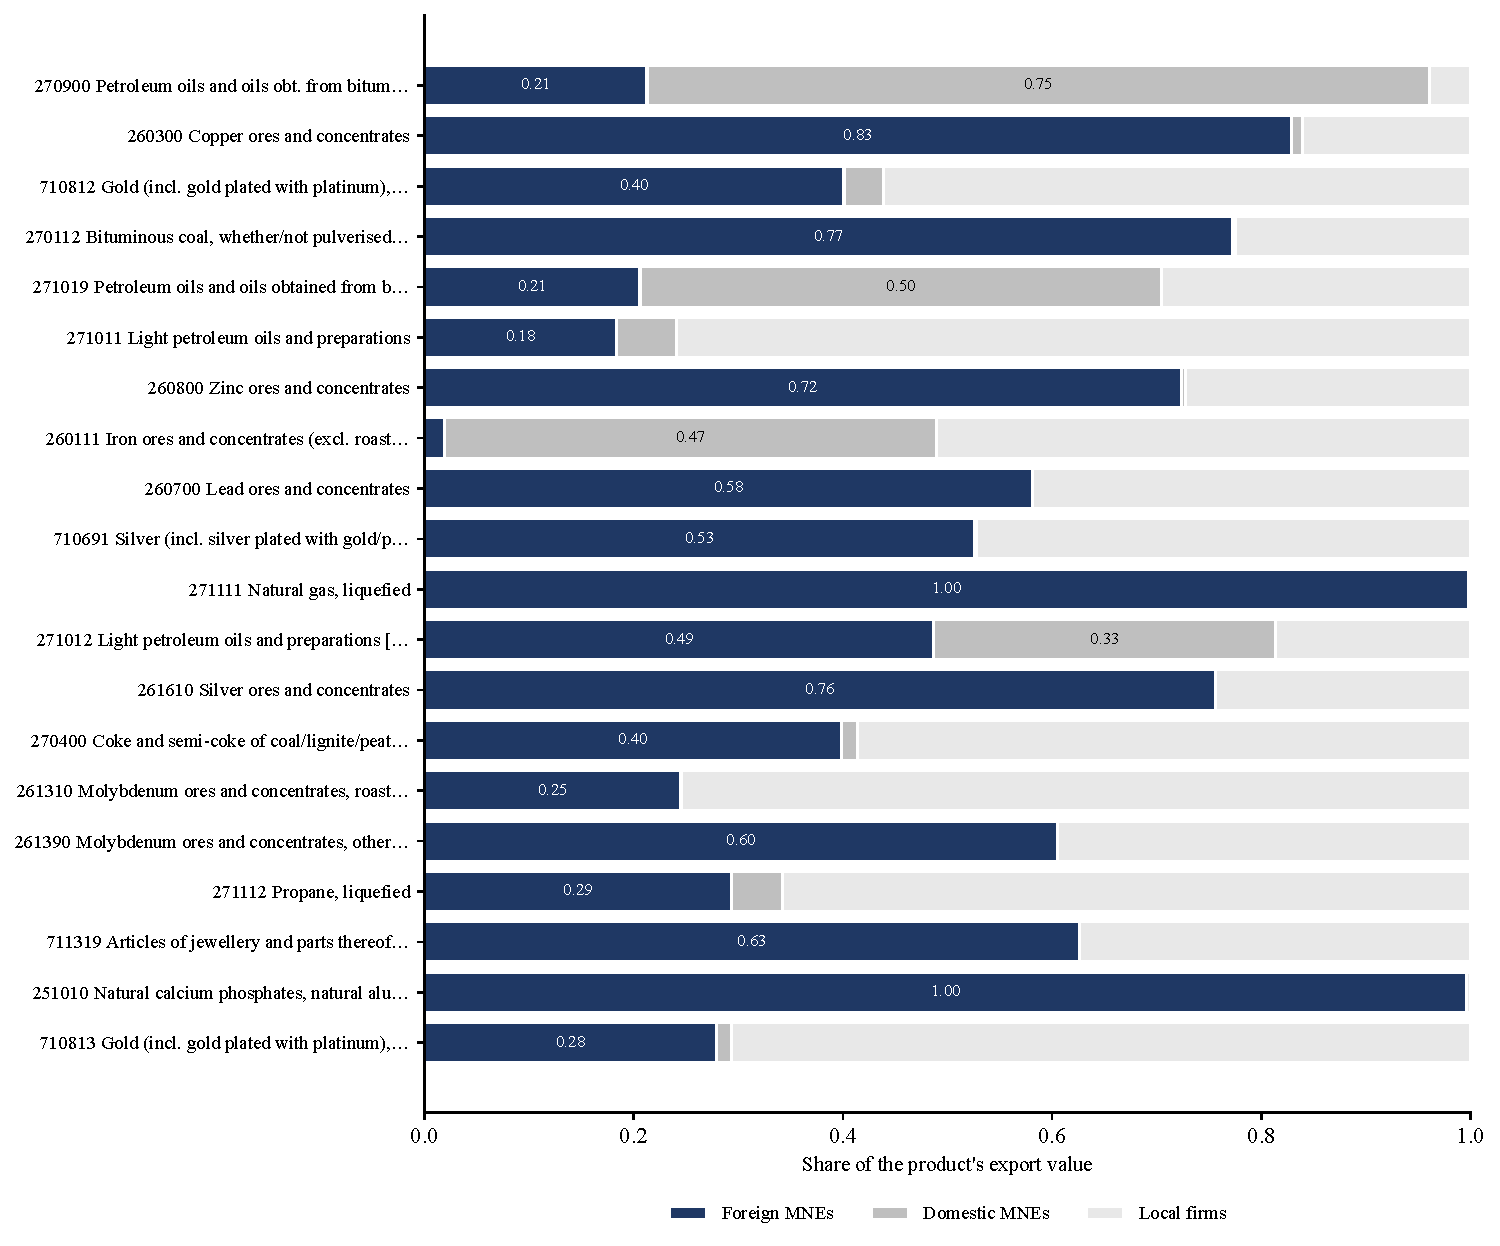
\includegraphics[width=1.0\textwidth,height=0.8\textheight,keepaspectratio]{figures/mining/fig_wp1f_top20_hs6_stacked.pdf}%
  \caption{Mining and Fuels: Ownership of the Twenty Largest Export Products}%
  \label{fig:hs_st_mining}%
  \par\vspace{2pt}%
  \parbox{0.92\textwidth}{\footnotesize %
  \textit{Notes:} Shares of each product's export value. Twenty largest HS6 products by export value.\\[3pt]%
  \textit{Source:} Authors' calculations based on customs data matched to Orbis and Dun \& Bradstreet.}%
  \end{figure}
% ---- Figure: Mining and Fuels: Ownership of the Twenty Largest Export Products, by Parent Country
\begin{figure}[H]\centering%
  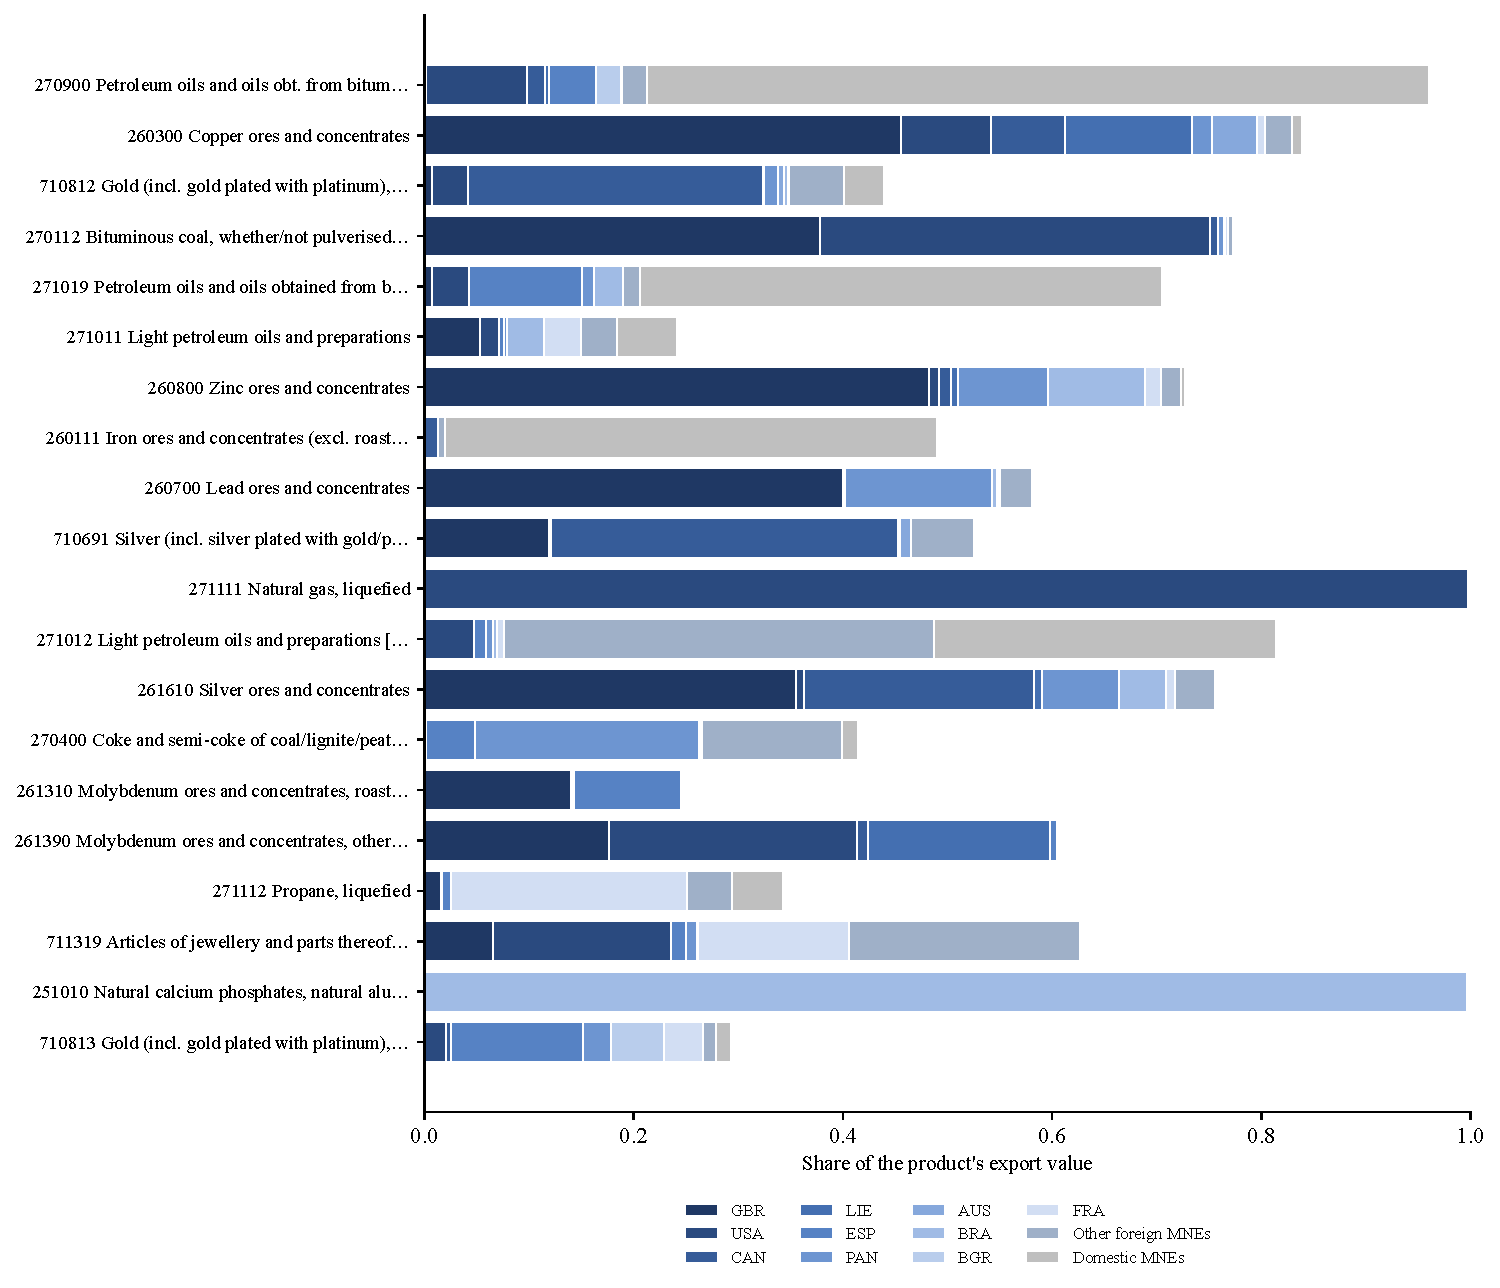
\includegraphics[width=1.0\textwidth,height=0.8\textheight,keepaspectratio]{figures/mining/fig_wp1f_top20_hs6_by_parent.pdf}%
  \caption{Mining and Fuels: Ownership of the Twenty Largest Export Products, by Parent Country}%
  \label{fig:hs_par_mining}%
  \par\vspace{2pt}%
  \parbox{0.92\textwidth}{\footnotesize %
  \textit{Notes:} Shares of each product's export value. Foreign-MNE share split by country of the ultimate parent; the unfilled part of each bar is local firms.\\[3pt]%
  \textit{Source:} Authors' calculations based on customs data matched to Orbis and Dun \& Bradstreet.}%
  \end{figure}
% ---- Figure: Mining and Fuels: Distribution of Export Value by Product-Level Foreign-Multinational Share
\begin{figure}[H]\centering%
  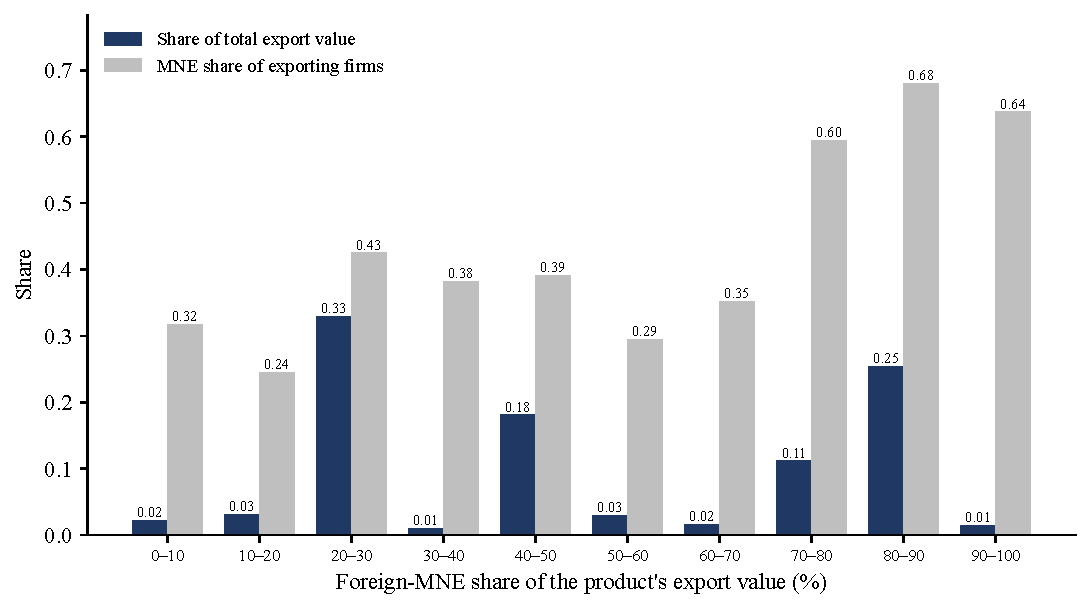
\includegraphics[width=0.85\textwidth,height=0.8\textheight,keepaspectratio]{figures/mining/fig_wp1f_foreign_share_distribution.pdf}%
  \caption{Mining and Fuels: Distribution of Export Value by Product-Level Foreign-Multinational Share}%
  \label{fig:hs_dist_mining}%
  \par\vspace{2pt}%
  \parbox{0.92\textwidth}{\footnotesize %
  \textit{Notes:} Share of mining and fuels export value and MNE share of exporting firms, by the foreign-MNE share of each HS6 product's export value.\\[3pt]%
  \textit{Source:} Authors' calculations based on customs data matched to Orbis and Dun \& Bradstreet.}%
  \end{figure}
% ---- Table: Mining and Fuels: Distribution of Export Value by Product-Level Foreign-Multinational Share
\begin{table}[H]\centering\small%
  \caption{Mining and Fuels: Distribution of Export Value by Product-Level Foreign-Multinational Share}%
  \label{tab:hs_dist_t_mining}%
  \adjustbox{max width=\textwidth, max totalheight=0.8\textheight}{\begin{tabular}{lrrr}
\toprule
Foreign share bin (\%) & Share of value & MNE share of exporting firms & HS6 products \\
\midrule
0--10 & 0.022 & 0.317 & 59 \\
10--20 & 0.031 & 0.245 & 34 \\
20--30 & 0.329 & 0.425 & 29 \\
30--40 & 0.011 & 0.382 & 15 \\
40--50 & 0.181 & 0.391 & 6 \\
50--60 & 0.029 & 0.294 & 20 \\
60--70 & 0.016 & 0.351 & 11 \\
70--80 & 0.112 & 0.595 & 7 \\
80--90 & 0.254 & 0.681 & 5 \\
90--100 & 0.015 & 0.637 & 22 \\
\bottomrule
\end{tabular}
}%
  \par\vspace{3pt}%
  \begin{minipage}{0.95\textwidth}\footnotesize %
  \textit{Notes:} Share of mining and fuels export value and MNE share of exporting firms, by the foreign-MNE share of each HS6 product's export value. MNE share of exporting firms: MNE firm--destination--product--year observations over all observations in the bin.\\[3pt]%
  \textit{Source:} Authors' calculations based on customs data matched to Orbis and Dun \& Bradstreet.%
  \end{minipage}%
  \end{table}
% ---- Figure: Mining and Fuels: Concentration of Exports across Products
\begin{figure}[H]\centering%
  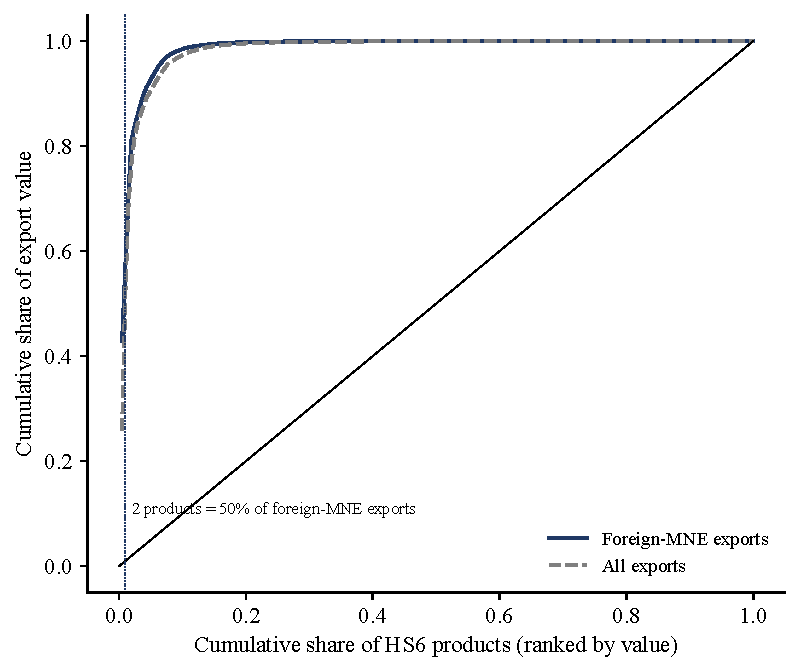
\includegraphics[width=0.6\textwidth,height=0.8\textheight,keepaspectratio]{figures/mining/fig_wp1f_lorenz_foreign.pdf}%
  \caption{Mining and Fuels: Concentration of Exports across Products}%
  \label{fig:hs_lor_mining}%
  \par\vspace{2pt}%
  \parbox{0.92\textwidth}{\footnotesize %
  \textit{Notes:} Cumulative share of export value against the cumulative share of HS6 products, ranked by value, for foreign-MNE exports and for all exports.\\[3pt]%
  \textit{Source:} Authors' calculations based on customs data matched to Orbis and Dun \& Bradstreet.}%
  \end{figure}
% ---- Table: Mining and Fuels: Exports and Multinational Shares, by HS Section
\begin{table}[H]\centering\footnotesize%
  \caption{Mining and Fuels: Exports and Multinational Shares, by HS Section}%
  \label{tab:hs_sec_mining}%
  \adjustbox{max width=\textwidth, max totalheight=0.8\textheight}{\begin{tabular}{@{}p{7.2cm} r r r r l@{}}
\toprule
HS section & US\$bn/yr & Foreign (\%) & Domestic (\%) & Local (\%) & Leading parent \\
\midrule
V Mineral products & 57.1 & 51 & 29 & 19 & GBR (0.42) \\
XIV Precious metals and stones & 15.3 & 41 & 4 & 56 & CAN (0.65) \\
\midrule
All sections & 72.4 & 49 & 25 & 26 & \\
\bottomrule
\end{tabular}
}%
  \par\vspace{3pt}%
  \begin{minipage}{0.95\textwidth}\footnotesize %
  \textit{Notes:} Foreign, domestic and local: percent of each section's export value. Leading parent: largest parent country and its share of the section's foreign-MNE exports. Values are annual averages in US\$ billion.\\[3pt]%
  \textit{Source:} Authors' calculations based on customs data matched to Orbis and Dun \& Bradstreet.%
  \end{minipage}%
  \end{table}
% ---- Table: Mining and Fuels: Thirty Largest Export Products
\begin{table}[H]\centering\footnotesize%
  \caption{Mining and Fuels: Thirty Largest Export Products}%
  \label{tab:hs_by_value_mining}%
  \adjustbox{max width=\textwidth, max totalheight=0.8\textheight}{\begin{tabular}{@{}l p{6.4cm} r r r r l@{}}
\toprule
HS6 & Description & US\$bn/yr & Foreign (\%) & Domestic (\%) & Local (\%) & Leading parent \\
\midrule
270900 & Petroleum oils and oils obt. from bituminous mins., crude & 17.9 & 21 & 75 & 4 & USA (0.45) \\
260300 & Copper ores and concentrates & 17.6 & 83 & 1 & 16 & GBR (0.55) \\
710812 & Gold (incl. gold plated with platinum), in unwrought forms (excl. powder) & 13.4 & 40 & 4 & 56 & CAN (0.70) \\
270112 & Bituminous coal, whether/\allowbreak{}not pulverised but not agglomerated & 5.7 & 77 & 0 & 23 & GBR (0.49) \\
271019 & Petroleum oils and oils obtained from bituminous minerals (other than crude) and preparations ... & 3.6 & 21 & 50 & 30 & ESP (0.52) \\
271011 & Light petroleum oils and preparations & 2.2 & 18 & 6 & 76 & GBR (0.29) \\
260800 & Zinc ores and concentrates & 1.5 & 72 & 0 & 27 & GBR (0.67) \\
260111 & Iron ores and concentrates (excl. roasted iron pyrites), non-agglomerated & 1.1 & 2 & 47 & 51 & CAN (0.65) \\
260700 & Lead ores and concentrates & 1.3 & 58 & 0 & 42 & GBR (0.69) \\
710691 & Silver (incl. silver plated with gold/\allowbreak{}platinum), unwrought & 0.8 & 53 & 0 & 47 & CAN (0.63) \\
271111 & Natural gas, liquefied & 0.9 & 100 & 0 & 0 & USA (1.00) \\
271012 & Light petroleum oils and preparations [HS2012 code] & 0.7 & 49 & 33 & 19 & CHL (0.80) \\
261610 & Silver ores and concentrates & 0.8 & 76 & 0 & 24 & GBR (0.47) \\
270400 & Coke and semi-coke of coal/\allowbreak{}lignite/\allowbreak{}peat, whether/\allowbreak{}not agglomerated; retort carbon & 0.6 & 40 & 2 & 59 & PAN (0.53) \\
261310 & Molybdenum ores and concentrates, roasted & 0.5 & 25 & 0 & 75 & GBR (0.57) \\
261390 & Molybdenum ores and concentrates, other than roasted & 0.6 & 60 & 0 & 40 & USA (0.39) \\
271112 & Propane, liquefied & 0.3 & 29 & 5 & 66 & FRA (0.77) \\
711319 & Articles of jewellery and parts thereof , of other precious metal (excl. silver), whether/\allowbreak{}not ... & 0.4 & 63 & 0 & 37 & BEL (0.27) \\
251010 & Natural calcium phosphates, natural aluminium calcium phosphates and phosphatic chalk, unground & 0.3 & 100 & 0 & 0 & BRA (1.00) \\
710813 & Gold (incl. gold plated with platinum), non-monetary, in semi-manufactured forms & 0.3 & 28 & 1 & 71 & ESP (0.45) \\
271121 & Natural gas, in gaseous state & 0.2 & 47 & 41 & 13 & USA (0.53) \\
271113 & Butanes, liquefied & 0.2 & 25 & 9 & 66 & FRA (0.83) \\
260112 & Iron ores and concentrates (excl. roasted iron pyrites), agglomerated & 0.1 & 7 & 88 & 4 & CHE (1.00) \\
710391 & Rubies, sapphires and emeralds, worked othw. than simply sawn/\allowbreak{}roughly shaped but not strung/\allowbreak{}mo... & 0.1 & 22 & 1 & 77 & BGR (0.67) \\
271600 & Electrical energy (optional heading) & 0.1 & 20 & 0 & 80 & CAN (0.82) \\
262099 & Ash and residues (excl. from the manufacture of iron/\allowbreak{}steel), n.e.s. in Ch.26 & 0.1 & 0 & 0 & 100 & CAN (0.89) \\
252329 & Portland cement (excl. white cement, whether/\allowbreak{}not artificially coloured), whether/\allowbreak{}not coloured & 0.1 & 68 & 10 & 22 & MEX (0.34) \\
250100 & Salt (incl. table salt and denatured salt) and pure sodium chloride, whether/\allowbreak{}not in aqueous so... & 0.1 & 62 & 8 & 29 & BEL (0.98) \\
271119 & Petroleum gases other than natural gas/\allowbreak{}propane/\allowbreak{}butanes/\allowbreak{}ethylene, propylene, butylene and butad... & 0.1 & 52 & 0 & 48 & FRA (0.38) \\
711291 & Waste and scrap of gold, incl. metal clad with gold but excl. sweepings containing other preci... & 0.1 & 18 & 0 & 81 & PAN (0.49) \\
\bottomrule
\end{tabular}
}%
  \par\vspace{3pt}%
  \begin{minipage}{0.95\textwidth}\footnotesize %
  \textit{Notes:} Thirty largest HS6 products by export value. Foreign, domestic and local: percent of the product's export value. Leading parent: largest parent country and its share of the product's foreign-MNE exports. Values are annual averages in US\$ billion.\\[3pt]%
  \textit{Source:} Authors' calculations based on customs data matched to Orbis and Dun \& Bradstreet.%
  \end{minipage}%
  \end{table}
% ---- Table: Mining and Fuels: Thirty Largest Export Products of Foreign Multinationals
\begin{table}[H]\centering\footnotesize%
  \caption{Mining and Fuels: Thirty Largest Export Products of Foreign Multinationals}%
  \label{tab:hs_by_foreign_value_mining}%
  \adjustbox{max width=\textwidth, max totalheight=0.8\textheight}{\begin{tabular}{@{}l p{6.4cm} r r r r l@{}}
\toprule
HS6 & Description & US\$bn/yr & Foreign (\%) & Domestic (\%) & Local (\%) & Leading parent \\
\midrule
260300 & Copper ores and concentrates & 17.6 & 83 & 1 & 16 & GBR (0.55) \\
710812 & Gold (incl. gold plated with platinum), in unwrought forms (excl. powder) & 13.4 & 40 & 4 & 56 & CAN (0.70) \\
270112 & Bituminous coal, whether/\allowbreak{}not pulverised but not agglomerated & 5.7 & 77 & 0 & 23 & GBR (0.49) \\
270900 & Petroleum oils and oils obt. from bituminous mins., crude & 17.9 & 21 & 75 & 4 & USA (0.45) \\
260800 & Zinc ores and concentrates & 1.5 & 72 & 0 & 27 & GBR (0.67) \\
271111 & Natural gas, liquefied & 0.9 & 100 & 0 & 0 & USA (1.00) \\
271019 & Petroleum oils and oils obtained from bituminous minerals (other than crude) and preparations ... & 3.6 & 21 & 50 & 30 & ESP (0.52) \\
260700 & Lead ores and concentrates & 1.3 & 58 & 0 & 42 & GBR (0.69) \\
261610 & Silver ores and concentrates & 0.8 & 76 & 0 & 24 & GBR (0.47) \\
710691 & Silver (incl. silver plated with gold/\allowbreak{}platinum), unwrought & 0.8 & 53 & 0 & 47 & CAN (0.63) \\
271012 & Light petroleum oils and preparations [HS2012 code] & 0.7 & 49 & 33 & 19 & CHL (0.80) \\
271011 & Light petroleum oils and preparations & 2.2 & 18 & 6 & 76 & GBR (0.29) \\
261390 & Molybdenum ores and concentrates, other than roasted & 0.6 & 60 & 0 & 40 & USA (0.39) \\
270400 & Coke and semi-coke of coal/\allowbreak{}lignite/\allowbreak{}peat, whether/\allowbreak{}not agglomerated; retort carbon & 0.6 & 40 & 2 & 59 & PAN (0.53) \\
251010 & Natural calcium phosphates, natural aluminium calcium phosphates and phosphatic chalk, unground & 0.3 & 100 & 0 & 0 & BRA (1.00) \\
711319 & Articles of jewellery and parts thereof , of other precious metal (excl. silver), whether/\allowbreak{}not ... & 0.4 & 63 & 0 & 37 & BEL (0.27) \\
261310 & Molybdenum ores and concentrates, roasted & 0.5 & 25 & 0 & 75 & GBR (0.57) \\
271121 & Natural gas, in gaseous state & 0.2 & 47 & 41 & 13 & USA (0.53) \\
271112 & Propane, liquefied & 0.3 & 29 & 5 & 66 & FRA (0.77) \\
252329 & Portland cement (excl. white cement, whether/\allowbreak{}not artificially coloured), whether/\allowbreak{}not coloured & 0.1 & 68 & 10 & 22 & MEX (0.34) \\
710813 & Gold (incl. gold plated with platinum), non-monetary, in semi-manufactured forms & 0.3 & 28 & 1 & 71 & ESP (0.45) \\
250100 & Salt (incl. table salt and denatured salt) and pure sodium chloride, whether/\allowbreak{}not in aqueous so... & 0.1 & 62 & 8 & 29 & BEL (0.98) \\
271113 & Butanes, liquefied & 0.2 & 25 & 9 & 66 & FRA (0.83) \\
271119 & Petroleum gases other than natural gas/\allowbreak{}propane/\allowbreak{}butanes/\allowbreak{}ethylene, propylene, butylene and butad... & 0.1 & 52 & 0 & 48 & FRA (0.38) \\
711311 & Articles of jewellery and parts thereof , of silver, whether/\allowbreak{}not plated/\allowbreak{}clad with other precio... & 0.1 & 65 & 0 & 35 & FRA (0.40) \\
711719 & Imitation jewellery, of base metal, whether/\allowbreak{}not plated with precious metal, other than cuff-li... & 0.0 & 63 & 3 & 34 & ALB (0.42) \\
710391 & Rubies, sapphires and emeralds, worked othw. than simply sawn/\allowbreak{}roughly shaped but not strung/\allowbreak{}mo... & 0.1 & 22 & 1 & 77 & BGR (0.67) \\
252310 & Cement clinkers & 0.0 & 56 & 0 & 44 & MEX (0.46) \\
271600 & Electrical energy (optional heading) & 0.1 & 20 & 0 & 80 & CAN (0.82) \\
260111 & Iron ores and concentrates (excl. roasted iron pyrites), non-agglomerated & 1.1 & 2 & 47 & 51 & CAN (0.65) \\
\bottomrule
\end{tabular}
}%
  \par\vspace{3pt}%
  \begin{minipage}{0.95\textwidth}\footnotesize %
  \textit{Notes:} Thirty largest HS6 products by foreign-MNE export value. Foreign, domestic and local: percent of the product's export value. Leading parent: largest parent country and its share of the product's foreign-MNE exports. Values are annual averages in US\$ billion.\\[3pt]%
  \textit{Source:} Authors' calculations based on customs data matched to Orbis and Dun \& Bradstreet.%
  \end{minipage}%
  \end{table}
% ---- Table: Mining and Fuels: Products with the Highest Foreign-Multinational Share
\begin{table}[H]\centering\footnotesize%
  \caption{Mining and Fuels: Products with the Highest Foreign-Multinational Share}%
  \label{tab:hs_by_foreign_share_mining}%
  \adjustbox{max width=\textwidth, max totalheight=0.8\textheight}{\begin{tabular}{@{}l p{6.4cm} r r r r l@{}}
\toprule
HS6 & Description & US\$bn/yr & Foreign (\%) & Domestic (\%) & Local (\%) & Leading parent \\
\midrule
271111 & Natural gas, liquefied & 0.9 & 100 & 0 & 0 & USA (1.00) \\
251010 & Natural calcium phosphates, natural aluminium calcium phosphates and phosphatic chalk, unground & 0.3 & 100 & 0 & 0 & BRA (1.00) \\
260300 & Copper ores and concentrates & 17.6 & 83 & 1 & 16 & GBR (0.55) \\
270112 & Bituminous coal, whether/\allowbreak{}not pulverised but not agglomerated & 5.7 & 77 & 0 & 23 & GBR (0.49) \\
261610 & Silver ores and concentrates & 0.8 & 76 & 0 & 24 & GBR (0.47) \\
260800 & Zinc ores and concentrates & 1.5 & 72 & 0 & 27 & GBR (0.67) \\
252329 & Portland cement (excl. white cement, whether/\allowbreak{}not artificially coloured), whether/\allowbreak{}not coloured & 0.1 & 68 & 10 & 22 & MEX (0.34) \\
711311 & Articles of jewellery and parts thereof , of silver, whether/\allowbreak{}not plated/\allowbreak{}clad with other precio... & 0.1 & 65 & 0 & 35 & FRA (0.40) \\
711719 & Imitation jewellery, of base metal, whether/\allowbreak{}not plated with precious metal, other than cuff-li... & 0.0 & 63 & 3 & 34 & ALB (0.42) \\
711319 & Articles of jewellery and parts thereof , of other precious metal (excl. silver), whether/\allowbreak{}not ... & 0.4 & 63 & 0 & 37 & BEL (0.27) \\
250100 & Salt (incl. table salt and denatured salt) and pure sodium chloride, whether/\allowbreak{}not in aqueous so... & 0.1 & 62 & 8 & 29 & BEL (0.98) \\
261390 & Molybdenum ores and concentrates, other than roasted & 0.6 & 60 & 0 & 40 & USA (0.39) \\
260700 & Lead ores and concentrates & 1.3 & 58 & 0 & 42 & GBR (0.69) \\
710691 & Silver (incl. silver plated with gold/\allowbreak{}platinum), unwrought & 0.8 & 53 & 0 & 47 & CAN (0.63) \\
271119 & Petroleum gases other than natural gas/\allowbreak{}propane/\allowbreak{}butanes/\allowbreak{}ethylene, propylene, butylene and butad... & 0.1 & 52 & 0 & 48 & FRA (0.38) \\
271012 & Light petroleum oils and preparations [HS2012 code] & 0.7 & 49 & 33 & 19 & CHL (0.80) \\
271121 & Natural gas, in gaseous state & 0.2 & 47 & 41 & 13 & USA (0.53) \\
710812 & Gold (incl. gold plated with platinum), in unwrought forms (excl. powder) & 13.4 & 40 & 4 & 56 & CAN (0.70) \\
270400 & Coke and semi-coke of coal/\allowbreak{}lignite/\allowbreak{}peat, whether/\allowbreak{}not agglomerated; retort carbon & 0.6 & 40 & 2 & 59 & PAN (0.53) \\
261690 & Precious metal ores and concentrates (excl. silver ores and concentrates) & 0.1 & 32 & 5 & 63 & PER (0.31) \\
271112 & Propane, liquefied & 0.3 & 29 & 5 & 66 & FRA (0.77) \\
710813 & Gold (incl. gold plated with platinum), non-monetary, in semi-manufactured forms & 0.3 & 28 & 1 & 71 & ESP (0.45) \\
271113 & Butanes, liquefied & 0.2 & 25 & 9 & 66 & FRA (0.83) \\
261310 & Molybdenum ores and concentrates, roasted & 0.5 & 25 & 0 & 75 & GBR (0.57) \\
710391 & Rubies, sapphires and emeralds, worked othw. than simply sawn/\allowbreak{}roughly shaped but not strung/\allowbreak{}mo... & 0.1 & 22 & 1 & 77 & BGR (0.67) \\
270900 & Petroleum oils and oils obt. from bituminous mins., crude & 17.9 & 21 & 75 & 4 & USA (0.45) \\
271019 & Petroleum oils and oils obtained from bituminous minerals (other than crude) and preparations ... & 3.6 & 21 & 50 & 30 & ESP (0.52) \\
271600 & Electrical energy (optional heading) & 0.1 & 20 & 0 & 80 & CAN (0.82) \\
711291 & Waste and scrap of gold, incl. metal clad with gold but excl. sweepings containing other preci... & 0.1 & 18 & 0 & 81 & PAN (0.49) \\
271011 & Light petroleum oils and preparations & 2.2 & 18 & 6 & 76 & GBR (0.29) \\
\bottomrule
\end{tabular}
}%
  \par\vspace{3pt}%
  \begin{minipage}{0.95\textwidth}\footnotesize %
  \textit{Notes:} HS6 products with exports of at least US\$500 million over the period, ranked by foreign-MNE share. Foreign, domestic and local: percent of the product's export value. Leading parent: largest parent country and its share of the product's foreign-MNE exports. Values are annual averages in US\$ billion.\\[3pt]%
  \textit{Source:} Authors' calculations based on customs data matched to Orbis and Dun \& Bradstreet.%
  \end{minipage}%
  \end{table}
% ---- Table: Mining and Fuels: Products with the Highest Domestic-Multinational Share
\begin{table}[H]\centering\footnotesize%
  \caption{Mining and Fuels: Products with the Highest Domestic-Multinational Share}%
  \label{tab:hs_by_domestic_share_mining}%
  \adjustbox{max width=\textwidth, max totalheight=0.8\textheight}{\begin{tabular}{@{}l p{6.4cm} r r r r l@{}}
\toprule
HS6 & Description & US\$bn/yr & Foreign (\%) & Domestic (\%) & Local (\%) & Leading parent \\
\midrule
260112 & Iron ores and concentrates (excl. roasted iron pyrites), agglomerated & 0.1 & 7 & 88 & 4 & CHE (1.00) \\
270900 & Petroleum oils and oils obt. from bituminous mins., crude & 17.9 & 21 & 75 & 4 & USA (0.45) \\
271019 & Petroleum oils and oils obtained from bituminous minerals (other than crude) and preparations ... & 3.6 & 21 & 50 & 30 & ESP (0.52) \\
260111 & Iron ores and concentrates (excl. roasted iron pyrites), non-agglomerated & 1.1 & 2 & 47 & 51 & CAN (0.65) \\
271121 & Natural gas, in gaseous state & 0.2 & 47 & 41 & 13 & USA (0.53) \\
271012 & Light petroleum oils and preparations [HS2012 code] & 0.7 & 49 & 33 & 19 & CHL (0.80) \\
271311 & Petroleum coke, not calcined & 0.0 & 6 & 23 & 71 & GBR (0.80) \\
252329 & Portland cement (excl. white cement, whether/\allowbreak{}not artificially coloured), whether/\allowbreak{}not coloured & 0.1 & 68 & 10 & 22 & MEX (0.34) \\
271113 & Butanes, liquefied & 0.2 & 25 & 9 & 66 & FRA (0.83) \\
250100 & Salt (incl. table salt and denatured salt) and pure sodium chloride, whether/\allowbreak{}not in aqueous so... & 0.1 & 62 & 8 & 29 & BEL (0.98) \\
271011 & Light petroleum oils and preparations & 2.2 & 18 & 6 & 76 & GBR (0.29) \\
261690 & Precious metal ores and concentrates (excl. silver ores and concentrates) & 0.1 & 32 & 5 & 63 & PER (0.31) \\
271112 & Propane, liquefied & 0.3 & 29 & 5 & 66 & FRA (0.77) \\
710812 & Gold (incl. gold plated with platinum), in unwrought forms (excl. powder) & 13.4 & 40 & 4 & 56 & CAN (0.70) \\
711719 & Imitation jewellery, of base metal, whether/\allowbreak{}not plated with precious metal, other than cuff-li... & 0.0 & 63 & 3 & 34 & ALB (0.42) \\
270400 & Coke and semi-coke of coal/\allowbreak{}lignite/\allowbreak{}peat, whether/\allowbreak{}not agglomerated; retort carbon & 0.6 & 40 & 2 & 59 & PAN (0.53) \\
710813 & Gold (incl. gold plated with platinum), non-monetary, in semi-manufactured forms & 0.3 & 28 & 1 & 71 & ESP (0.45) \\
710391 & Rubies, sapphires and emeralds, worked othw. than simply sawn/\allowbreak{}roughly shaped but not strung/\allowbreak{}mo... & 0.1 & 22 & 1 & 77 & BGR (0.67) \\
260300 & Copper ores and concentrates & 17.6 & 83 & 1 & 16 & GBR (0.55) \\
711291 & Waste and scrap of gold, incl. metal clad with gold but excl. sweepings containing other preci... & 0.1 & 18 & 0 & 81 & PAN (0.49) \\
260800 & Zinc ores and concentrates & 1.5 & 72 & 0 & 27 & GBR (0.67) \\
270112 & Bituminous coal, whether/\allowbreak{}not pulverised but not agglomerated & 5.7 & 77 & 0 & 23 & GBR (0.49) \\
710691 & Silver (incl. silver plated with gold/\allowbreak{}platinum), unwrought & 0.8 & 53 & 0 & 47 & CAN (0.63) \\
711311 & Articles of jewellery and parts thereof , of silver, whether/\allowbreak{}not plated/\allowbreak{}clad with other precio... & 0.1 & 65 & 0 & 35 & FRA (0.40) \\
271119 & Petroleum gases other than natural gas/\allowbreak{}propane/\allowbreak{}butanes/\allowbreak{}ethylene, propylene, butylene and butad... & 0.1 & 52 & 0 & 48 & FRA (0.38) \\
711319 & Articles of jewellery and parts thereof , of other precious metal (excl. silver), whether/\allowbreak{}not ... & 0.4 & 63 & 0 & 37 & BEL (0.27) \\
261310 & Molybdenum ores and concentrates, roasted & 0.5 & 25 & 0 & 75 & GBR (0.57) \\
251010 & Natural calcium phosphates, natural aluminium calcium phosphates and phosphatic chalk, unground & 0.3 & 100 & 0 & 0 & BRA (1.00) \\
260700 & Lead ores and concentrates & 1.3 & 58 & 0 & 42 & GBR (0.69) \\
262099 & Ash and residues (excl. from the manufacture of iron/\allowbreak{}steel), n.e.s. in Ch.26 & 0.1 & 0 & 0 & 100 & CAN (0.89) \\
\bottomrule
\end{tabular}
}%
  \par\vspace{3pt}%
  \begin{minipage}{0.95\textwidth}\footnotesize %
  \textit{Notes:} HS6 products with exports of at least US\$500 million over the period, ranked by domestic-MNE share. Foreign, domestic and local: percent of the product's export value. Leading parent: largest parent country and its share of the product's foreign-MNE exports. Values are annual averages in US\$ billion.\\[3pt]%
  \textit{Source:} Authors' calculations based on customs data matched to Orbis and Dun \& Bradstreet.%
  \end{minipage}%
  \end{table}

\section{Product Groups within the Sector}\label{sec:sub_mining}

\subsection{By HS Section}
% ---- Table: Mining and Fuels: Exports and Multinational Shares, by HS Section
\begin{table}[H]\centering\footnotesize%
  \caption{Mining and Fuels: Exports and Multinational Shares, by HS Section}%
  \label{tab:sc_hs_section_mining}%
  \adjustbox{max width=\textwidth, max totalheight=0.8\textheight}{\begin{tabular}{@{}l r r r r l@{}}
\toprule
HS section & Total exports (US\$bn/yr) & MNE exports (US\$bn/yr) & Foreign (\%) & Domestic (\%) & Leading parents (share of foreign) \\
\midrule
V Mineral products & 57.1 & 45.4 & 51.1 & 29.5 & GBR 0.42, USA 0.23, LIE 0.08 \\
XIV Precious metals and stones & 15.3 & 7.0 & 40.8 & 3.5 & CAN 0.65, USA 0.09, GBR 0.04 \\
\midrule
All & 72.4 & 52.4 & 49.2 & 24.5 & \\
\bottomrule
\end{tabular}
}%
  \par\vspace{3pt}%
  \begin{minipage}{0.95\textwidth}\footnotesize %
  \textit{Notes:} HS sections. Foreign and domestic: percent of the group's export value. Leading parents: the three largest parent countries and their share of the row's foreign-MNE exports. Values are annual averages in US\$ billion.\\[3pt]%
  \textit{Source:} Authors' calculations based on customs data matched to Orbis and Dun \& Bradstreet.%
  \end{minipage}%
  \end{table}
% ---- Figure: Mining and Fuels: Multinational Share of Export Value, by HS Section
\begin{figure}[H]\centering%
  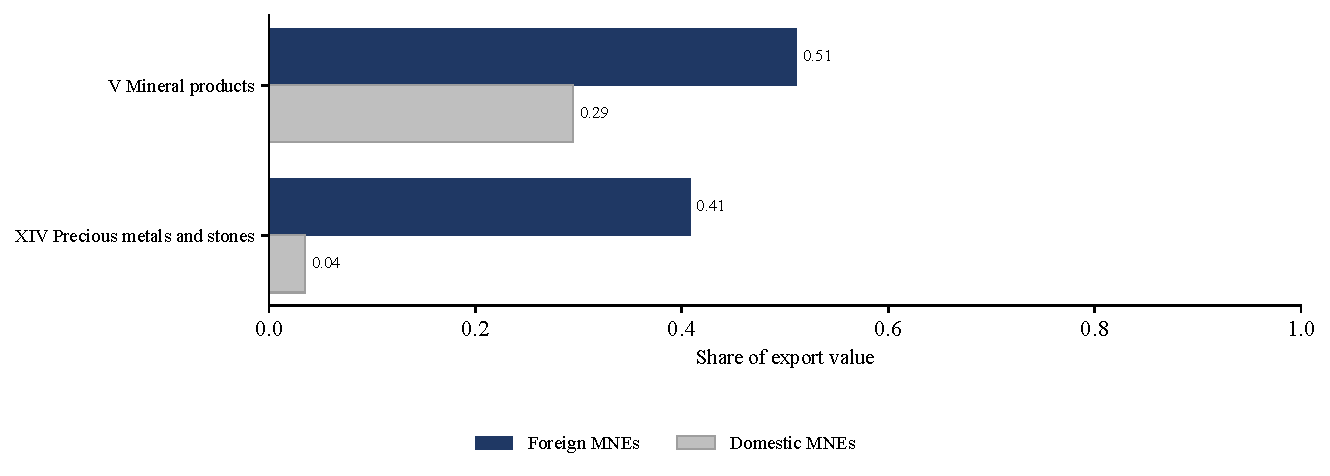
\includegraphics[width=0.9\textwidth,height=0.8\textheight,keepaspectratio]{figures/mining/fig_wp2_hs_section.pdf}%
  \caption{Mining and Fuels: Multinational Share of Export Value, by HS Section}%
  \label{fig:sc_hs_section_f_mining}%
  \par\vspace{2pt}%
  \parbox{0.92\textwidth}{\footnotesize %
  \textit{Notes:} Shares of mining and fuels export value (HS 25--27 and 71), all available years pooled. HS sections.\\[3pt]%
  \textit{Source:} Authors' calculations based on customs data matched to Orbis and Dun \& Bradstreet.}%
  \end{figure}
% ---- Figure: Mining and Fuels: Foreign-Multinational Share of Export Value, by Exporting Country and HS Section
\begin{figure}[H]\centering%
  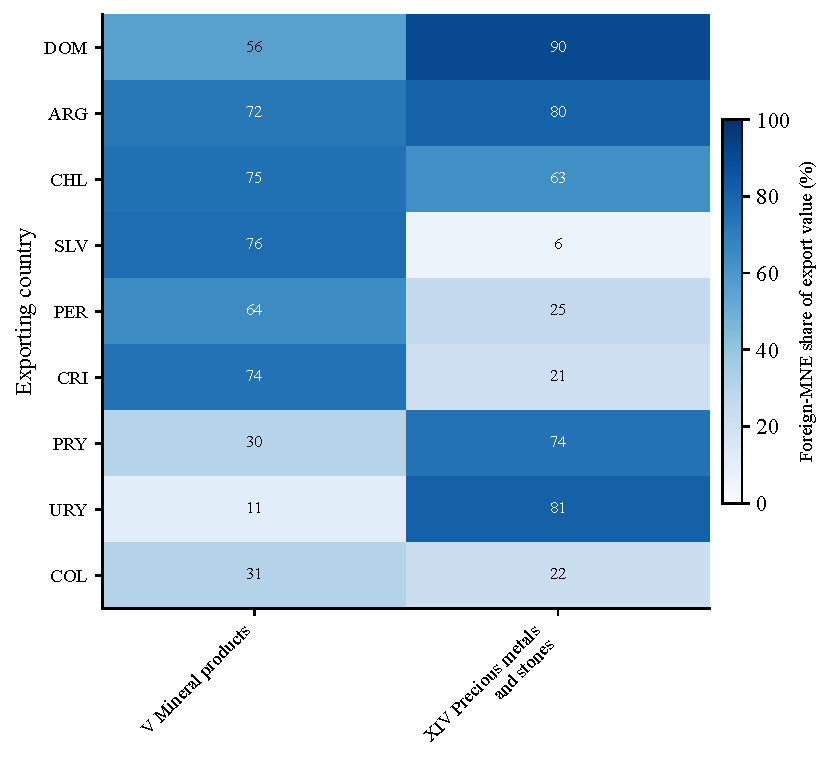
\includegraphics[width=0.95\textwidth,height=0.8\textheight,keepaspectratio]{figures/mining/fig_wp2_origin_x_hs_section.pdf}%
  \caption{Mining and Fuels: Foreign-Multinational Share of Export Value, by Exporting Country and HS Section}%
  \label{fig:sc_hs_section_hm_mining}%
  \par\vspace{2pt}%
  \parbox{0.92\textwidth}{\footnotesize %
  \textit{Notes:} Percent of each group's export value in each country shipped by foreign MNEs. HS sections.\\[3pt]%
  \textit{Source:} Authors' calculations based on customs data matched to Orbis and Dun \& Bradstreet.}%
  \end{figure}
% ---- Table: Mining and Fuels: Exports by Exporting Country and HS Section
\begin{table}[H]\centering\footnotesize%
  \caption{Mining and Fuels: Exports by Exporting Country and HS Section}%
  \label{tab:sc_hs_section_ht_mining}%
  \adjustbox{max width=\textwidth, max totalheight=0.8\textheight}{\begin{tabular}{lrrr}
\toprule
Origin & V Mineral products & XIV Precious metals and stones & All \\
\midrule
\multicolumn{4}{l}{\textit{Panel A: composition of the origin's exports, \% (rows sum to 100)}} \\
ARG & 63.5 & 36.5 & 100.0 \\
CHL & 92.8 & 7.2 & 100.0 \\
COL & 91.5 & 8.5 & 100.0 \\
CRI & 48.3 & 51.7 & 100.0 \\
DOM & 13.9 & 86.1 & 100.0 \\
PER & 68.8 & 31.2 & 100.0 \\
PRY & 67.9 & 32.1 & 100.0 \\
SLV & 74.8 & 25.2 & 100.0 \\
URY & 54.1 & 45.9 & 100.0 \\
All origins & 80.9 & 19.1 & 100.0 \\
\midrule
\multicolumn{4}{l}{\textit{Panel B: foreign-MNE share of export value, \%}} \\
ARG & 72.2 & 80.2 & 75.1 \\
CHL & 74.7 & 63.1 & 73.9 \\
COL & 30.8 & 22.4 & 30.1 \\
CRI & 74.4 & 21.1 & 46.9 \\
DOM & 55.7 & 90.1 & 85.3 \\
PER & 64.5 & 25.1 & 52.2 \\
PRY & 29.9 & 74.3 & 44.1 \\
SLV & 76.5 & 6.2 & 58.8 \\
URY & 10.6 & 81.0 & 42.9 \\
All origins & 51.1 & 40.8 & 49.2 \\
\bottomrule
\end{tabular}
}%
  \par\vspace{3pt}%
  \begin{minipage}{0.95\textwidth}\footnotesize %
  \textit{Notes:} Panel A: composition of each country's exports in the sector (rows add to 100). Panel B: percent of each cell's export value shipped by foreign MNEs. HS sections.\\[3pt]%
  \textit{Source:} Authors' calculations based on customs data matched to Orbis and Dun \& Bradstreet.%
  \end{minipage}%
  \end{table}
% ---- Table: Mining and Fuels: Exports by HS Section and Parent Country
\begin{table}[H]\centering\footnotesize%
  \caption{Mining and Fuels: Exports by HS Section and Parent Country}%
  \label{tab:sc_hs_section_par_mining}%
  \adjustbox{max width=\textwidth, max totalheight=0.8\textheight}{\begin{tabular}{lrrrrrrrrrrrr}
\toprule
HS section & GBR & USA & CAN & LIE & ESP & PAN & AUS & BRA & BGR & FRA & Other & Domestic \\
\midrule
V Mineral products & 20.7 & 11.5 & 3.1 & 4.1 & 1.9 & 1.3 & 1.3 & 0.9 & 0.8 & 0.6 & 4.8 & 29.5 \\
XIV Precious metals and stones & 1.5 & 3.3 & 25.1 & 0.0 & 0.4 & 1.3 & 0.5 & 0.4 & 0.2 & 0.5 & 7.6 & 3.5 \\
\bottomrule
\end{tabular}
}%
  \par\vspace{3pt}%
  \begin{minipage}{0.95\textwidth}\footnotesize %
  \textit{Notes:} Percent of each group's export value, by country of the ultimate parent of foreign MNEs; domestic MNEs shown for comparison. HS sections.\\[3pt]%
  \textit{Source:} Authors' calculations based on customs data matched to Orbis and Dun \& Bradstreet.%
  \end{minipage}%
  \end{table}

\subsection{By End Use}
% ---- Table: Mining and Fuels: Exports and Multinational Shares, by End Use
\begin{table}[H]\centering\footnotesize%
  \caption{Mining and Fuels: Exports and Multinational Shares, by End Use}%
  \label{tab:sc_bec_enduse_mining}%
  \adjustbox{max width=\textwidth, max totalheight=0.8\textheight}{\begin{tabular}{@{}l r r r r l@{}}
\toprule
BEC end use & Total exports (US\$bn/yr) & MNE exports (US\$bn/yr) & Foreign (\%) & Domestic (\%) & Leading parents (share of foreign) \\
\midrule
Intermediate & 65.4 & 48.6 & 51.6 & 23.7 & GBR 0.37, USA 0.21, CAN 0.16 \\
Consumption & 0.5 & 0.3 & 61.7 & 0.4 & USA 0.22, FRA 0.22, BEL 0.21 \\
Capital & 0.0 & 0.0 & 21.4 & 0.0 & FRA 0.82, USA 0.08, GBR 0.03 \\
\midrule
All & 65.9 & 48.9 & 51.6 & 23.6 & \\
\bottomrule
\end{tabular}
}%
  \par\vspace{3pt}%
  \begin{minipage}{0.95\textwidth}\footnotesize %
  \textit{Notes:} End use from BEC Rev.\,4. Foreign and domestic: percent of the group's export value. Leading parents: the three largest parent countries and their share of the row's foreign-MNE exports. Values are annual averages in US\$ billion.\\[3pt]%
  \textit{Source:} Authors' calculations based on customs data matched to Orbis and Dun \& Bradstreet.%
  \end{minipage}%
  \end{table}
% ---- Figure: Mining and Fuels: Multinational Share of Export Value, by End Use
\begin{figure}[H]\centering%
  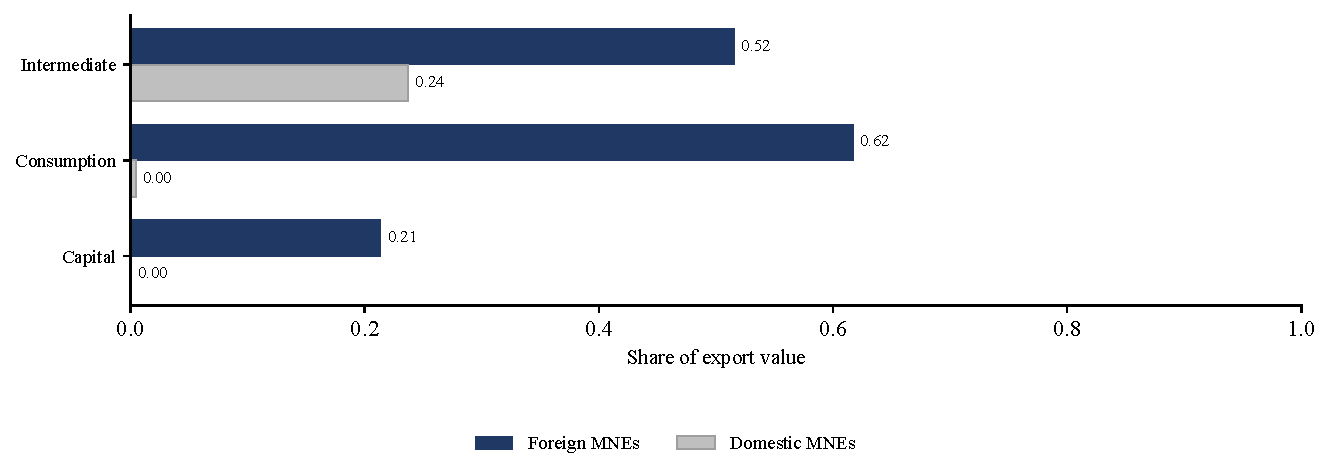
\includegraphics[width=0.9\textwidth,height=0.8\textheight,keepaspectratio]{figures/mining/fig_wp2_bec_enduse.pdf}%
  \caption{Mining and Fuels: Multinational Share of Export Value, by End Use}%
  \label{fig:sc_bec_enduse_f_mining}%
  \par\vspace{2pt}%
  \parbox{0.92\textwidth}{\footnotesize %
  \textit{Notes:} Shares of mining and fuels export value (HS 25--27 and 71), all available years pooled. End use from BEC Rev.\,4.\\[3pt]%
  \textit{Source:} Authors' calculations based on customs data matched to Orbis and Dun \& Bradstreet.}%
  \end{figure}
% ---- Figure: Mining and Fuels: Foreign-Multinational Share of Export Value, by Exporting Country and End Use
\begin{figure}[H]\centering%
  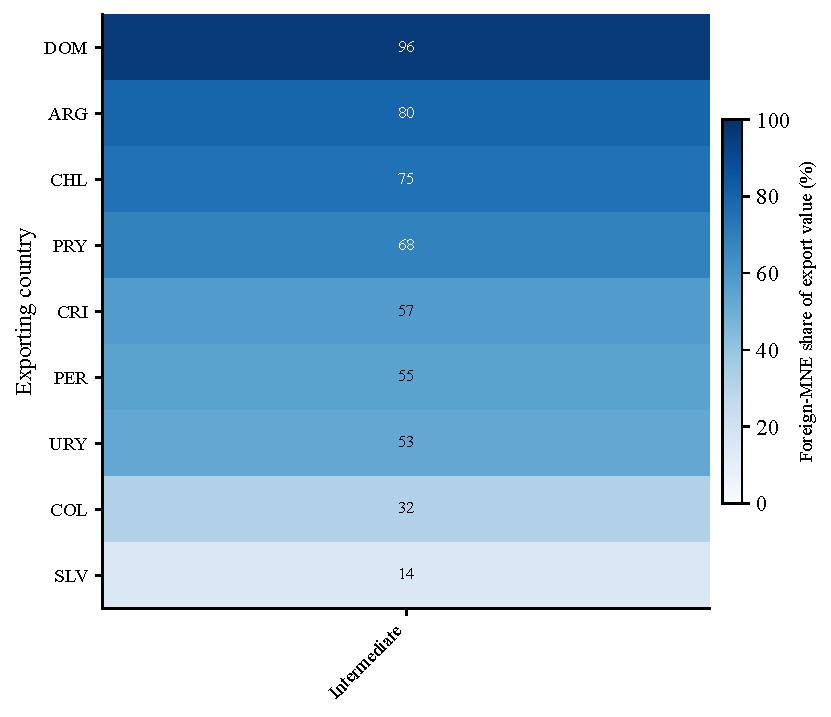
\includegraphics[width=0.95\textwidth,height=0.8\textheight,keepaspectratio]{figures/mining/fig_wp2_origin_x_bec_enduse.pdf}%
  \caption{Mining and Fuels: Foreign-Multinational Share of Export Value, by Exporting Country and End Use}%
  \label{fig:sc_bec_enduse_hm_mining}%
  \par\vspace{2pt}%
  \parbox{0.92\textwidth}{\footnotesize %
  \textit{Notes:} Percent of each group's export value in each country shipped by foreign MNEs. End use from BEC Rev.\,4.\\[3pt]%
  \textit{Source:} Authors' calculations based on customs data matched to Orbis and Dun \& Bradstreet.}%
  \end{figure}
% ---- Table: Mining and Fuels: Exports by Exporting Country and End Use
\begin{table}[H]\centering\footnotesize%
  \caption{Mining and Fuels: Exports by Exporting Country and End Use}%
  \label{tab:sc_bec_enduse_ht_mining}%
  \adjustbox{max width=\textwidth, max totalheight=0.8\textheight}{\begin{tabular}{lrrrr}
\toprule
Origin & Intermediate & Consumption & Capital & All \\
\midrule
\multicolumn{5}{l}{\textit{Panel A: composition of the origin's exports, \% (rows sum to 100)}} \\
ARG & 100.0 & 0.0 & 0.0 & 100.0 \\
CHL & 100.0 & 0.0 & 0.0 & 100.0 \\
COL & 99.9 & 0.1 & 0.0 & 100.0 \\
CRI & 82.5 & 17.5 & 0.1 & 100.0 \\
DOM & 81.9 & 18.1 & 0.0 & 100.0 \\
PER & 99.6 & 0.4 & 0.0 & 100.0 \\
PRY & 98.1 & 0.1 & 1.8 & 100.0 \\
SLV & 95.4 & 4.6 & 0.0 & 100.0 \\
URY & 99.4 & 0.6 & 0.0 & 100.0 \\
All origins & 99.4 & 0.6 & 0.0 & 100.0 \\
\midrule
\multicolumn{5}{l}{\textit{Panel B: foreign-MNE share of export value, \%}} \\
ARG & 79.7 & 11.4 & 97.0 & 79.6 \\
CHL & 74.8 & 24.4 & 28.6 & 74.8 \\
COL & 31.7 & 68.0 & 22.0 & 31.8 \\
CRI & 57.5 & 44.6 & 96.4 & 55.2 \\
DOM & 96.1 & 57.9 & 0.0 & 89.2 \\
PER & 54.7 & 77.2 & 0.2 & 54.8 \\
PRY & 68.2 & 14.8 & 100.0 & 68.8 \\
SLV & 14.4 & 0.4 & 0.0 & 13.7 \\
URY & 52.7 & 69.3 & 58.2 & 52.8 \\
All origins & 51.6 & 61.7 & 21.4 & 51.6 \\
\bottomrule
\end{tabular}
}%
  \par\vspace{3pt}%
  \begin{minipage}{0.95\textwidth}\footnotesize %
  \textit{Notes:} Panel A: composition of each country's exports in the sector (rows add to 100). Panel B: percent of each cell's export value shipped by foreign MNEs. End use from BEC Rev.\,4.\\[3pt]%
  \textit{Source:} Authors' calculations based on customs data matched to Orbis and Dun \& Bradstreet.%
  \end{minipage}%
  \end{table}
% ---- Table: Mining and Fuels: Exports by End Use and Parent Country
\begin{table}[H]\centering\footnotesize%
  \caption{Mining and Fuels: Exports by End Use and Parent Country}%
  \label{tab:sc_bec_enduse_par_mining}%
  \adjustbox{max width=\textwidth, max totalheight=0.8\textheight}{\begin{tabular}{lrrrrrrrrrrrr}
\toprule
BEC end use & GBR & USA & CAN & LIE & ESP & PAN & AUS & BRA & BGR & FRA & Other & Domestic \\
\midrule
Intermediate & 18.6 & 10.6 & 8.1 & 3.6 & 1.4 & 1.4 & 1.3 & 0.7 & 0.8 & 0.5 & 4.5 & 23.7 \\
Consumption & 6.2 & 13.4 & 0.0 & 0.0 & 2.2 & 2.6 & 0.0 & 0.1 & 0.0 & 13.3 & 23.9 & 0.4 \\
Capital & 0.7 & 1.8 & 0.0 & 0.0 & 0.1 & 0.0 & 0.0 & 0.0 & 0.0 & 17.5 & 1.2 & 0.0 \\
\bottomrule
\end{tabular}
}%
  \par\vspace{3pt}%
  \begin{minipage}{0.95\textwidth}\footnotesize %
  \textit{Notes:} Percent of each group's export value, by country of the ultimate parent of foreign MNEs; domestic MNEs shown for comparison. End use from BEC Rev.\,4.\\[3pt]%
  \textit{Source:} Authors' calculations based on customs data matched to Orbis and Dun \& Bradstreet.%
  \end{minipage}%
  \end{table}

\subsection{By BEC Category}
% ---- Table: Mining and Fuels: Exports and Multinational Shares, by BEC Category
\begin{table}[H]\centering\footnotesize%
  \caption{Mining and Fuels: Exports and Multinational Shares, by BEC Category}%
  \label{tab:sc_bec4_mining}%
  \adjustbox{max width=\textwidth, max totalheight=0.8\textheight}{\begin{tabular}{@{}l r r r r l@{}}
\toprule
BEC Rev.\,4 category & Total exports (US\$bn/yr) & MNE exports (US\$bn/yr) & Foreign (\%) & Domestic (\%) & Leading parents (share of foreign) \\
\midrule
31 Fuels, primary & 23.8 & 21.7 & 35.1 & 56.3 & USA 0.47, GBR 0.27, ESP 0.10 \\
21 Industrial supplies, primary & 24.3 & 18.6 & 73.7 & 3.7 & GBR 0.54, LIE 0.13, USA 0.10 \\
22 Industrial supplies, processed & 15.1 & 6.9 & 40.4 & 3.8 & CAN 0.67, USA 0.08, GBR 0.03 \\
32 32 & 5.8 & 3.0 & 19.8 & 34.7 & ESP 0.34, BRA 0.15, USA 0.14 \\
322 Fuels, other processed & 2.2 & 1.4 & 58.3 & 2.0 & USA 0.76, FRA 0.12, PAN 0.02 \\
Other & 0.5 & 0.3 & 61.2 & 0.8 & FRA 0.22, USA 0.22, BEL 0.21 \\
\midrule
All & 71.7 & 51.9 & 49.2 & 24.5 & \\
\bottomrule
\end{tabular}
}%
  \par\vspace{3pt}%
  \begin{minipage}{0.95\textwidth}\footnotesize %
  \textit{Notes:} Categories of BEC Rev.\,4. Foreign and domestic: percent of the group's export value. Leading parents: the three largest parent countries and their share of the row's foreign-MNE exports. Values are annual averages in US\$ billion.\\[3pt]%
  \textit{Source:} Authors' calculations based on customs data matched to Orbis and Dun \& Bradstreet.%
  \end{minipage}%
  \end{table}
% ---- Figure: Mining and Fuels: Multinational Share of Export Value, by BEC Category
\begin{figure}[H]\centering%
  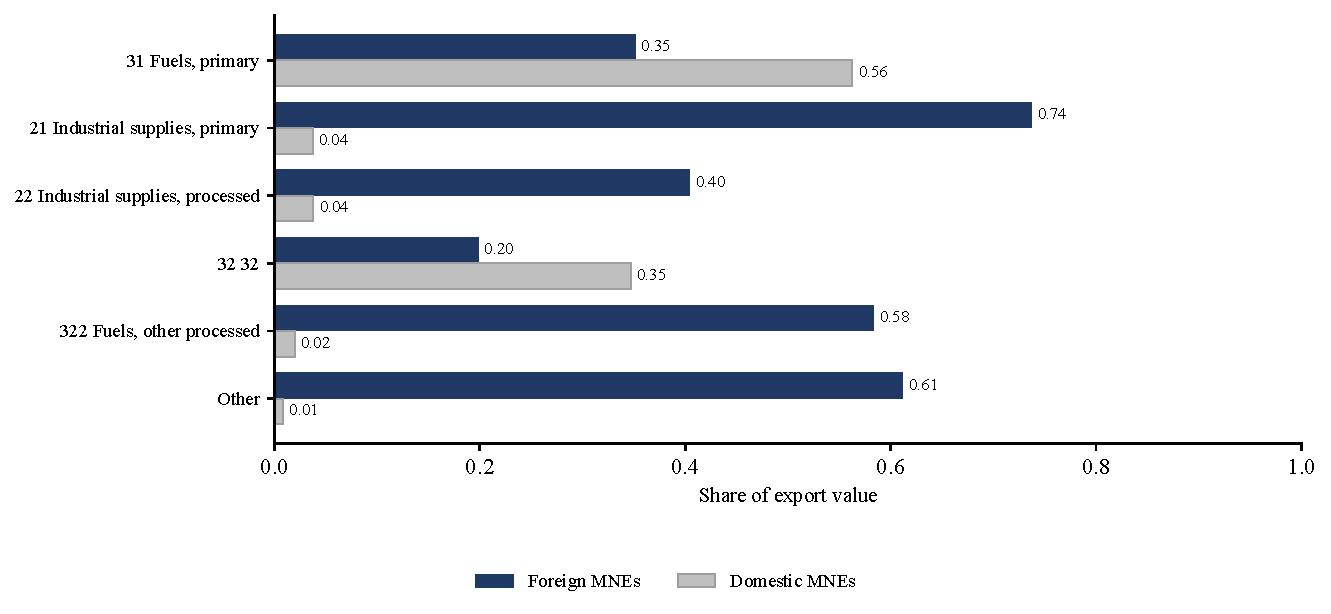
\includegraphics[width=0.9\textwidth,height=0.8\textheight,keepaspectratio]{figures/mining/fig_wp2_bec4.pdf}%
  \caption{Mining and Fuels: Multinational Share of Export Value, by BEC Category}%
  \label{fig:sc_bec4_f_mining}%
  \par\vspace{2pt}%
  \parbox{0.92\textwidth}{\footnotesize %
  \textit{Notes:} Shares of mining and fuels export value (HS 25--27 and 71), all available years pooled. Categories of BEC Rev.\,4.\\[3pt]%
  \textit{Source:} Authors' calculations based on customs data matched to Orbis and Dun \& Bradstreet.}%
  \end{figure}
% ---- Figure: Mining and Fuels: Foreign-Multinational Share of Export Value, by Exporting Country and BEC Category
\begin{figure}[H]\centering%
  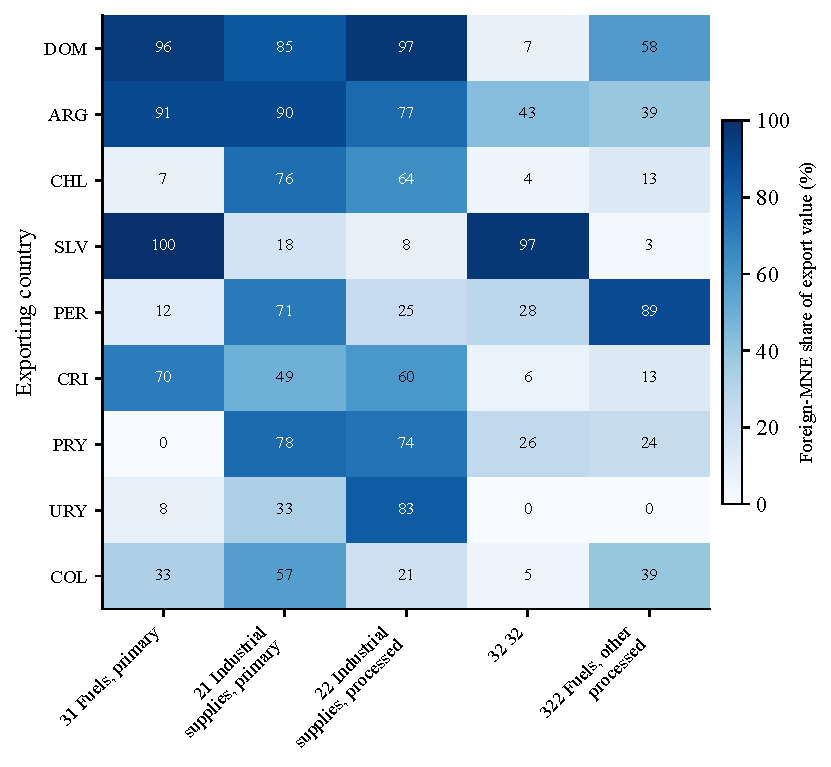
\includegraphics[width=0.95\textwidth,height=0.8\textheight,keepaspectratio]{figures/mining/fig_wp2_origin_x_bec4.pdf}%
  \caption{Mining and Fuels: Foreign-Multinational Share of Export Value, by Exporting Country and BEC Category}%
  \label{fig:sc_bec4_hm_mining}%
  \par\vspace{2pt}%
  \parbox{0.92\textwidth}{\footnotesize %
  \textit{Notes:} Percent of each group's export value in each country shipped by foreign MNEs. Categories of BEC Rev.\,4.\\[3pt]%
  \textit{Source:} Authors' calculations based on customs data matched to Orbis and Dun \& Bradstreet.}%
  \end{figure}
% ---- Table: Mining and Fuels: Exports by Exporting Country and BEC Category
\begin{table}[H]\centering\footnotesize%
  \caption{Mining and Fuels: Exports by Exporting Country and BEC Category}%
  \label{tab:sc_bec4_ht_mining}%
  \adjustbox{max width=\textwidth, max totalheight=0.8\textheight}{\begin{tabular}{lrrrrrrr}
\toprule
Origin & 31 Fuels, primary & 21 Industrial supplies, primary & 22 Industrial supplies, processed & 32 32 & 322 Fuels, other processed & Other & All \\
\midrule
\multicolumn{8}{l}{\textit{Panel A: composition of the origin's exports, \% (rows sum to 100)}} \\
ARG & 23.4 & 17.4 & 38.8 & 12.0 & 8.3 & 0.0 & 100.0 \\
CHL & 0.2 & 91.3 & 7.2 & 1.1 & 0.2 & 0.0 & 100.0 \\
COL & 80.4 & 0.4 & 8.6 & 8.1 & 2.4 & 0.1 & 100.0 \\
CRI & 0.0 & 15.8 & 57.0 & 11.5 & 0.2 & 15.5 & 100.0 \\
DOM & 0.0 & 5.1 & 72.7 & 4.8 & 0.2 & 17.2 & 100.0 \\
PER & 1.3 & 53.7 & 31.0 & 9.8 & 3.8 & 0.4 & 100.0 \\
PRY & 0.0 & 4.9 & 31.3 & 58.0 & 5.0 & 0.8 & 100.0 \\
SLV & 0.4 & 27.3 & 9.0 & 54.4 & 6.9 & 2.1 & 100.0 \\
URY & 0.0 & 10.1 & 47.1 & 18.8 & 23.4 & 0.5 & 100.0 \\
All origins & 35.0 & 34.8 & 19.1 & 7.8 & 2.9 & 0.5 & 100.0 \\
\midrule
\multicolumn{8}{l}{\textit{Panel B: foreign-MNE share of export value, \%}} \\
ARG & 90.5 & 89.8 & 77.4 & 43.2 & 38.7 & 11.9 & 75.3 \\
CHL & 7.4 & 76.0 & 63.5 & 4.1 & 13.0 & 8.3 & 74.1 \\
COL & 32.5 & 56.8 & 21.1 & 4.6 & 39.1 & 67.8 & 29.6 \\
CRI & 70.5 & 49.1 & 59.8 & 6.3 & 12.6 & 44.9 & 49.6 \\
DOM & 95.6 & 84.9 & 97.0 & 7.2 & 58.1 & 57.9 & 85.3 \\
PER & 12.0 & 70.7 & 24.7 & 27.8 & 89.4 & 75.5 & 52.2 \\
PRY & 0.0 & 77.7 & 73.8 & 26.3 & 24.4 & 94.8 & 44.1 \\
SLV & 99.8 & 18.3 & 8.0 & 96.9 & 2.5 & 0.4 & 58.9 \\
URY & 8.2 & 33.3 & 82.9 & 0.2 & 0.1 & 68.3 & 42.9 \\
All origins & 35.1 & 73.7 & 40.4 & 19.8 & 58.3 & 61.2 & 49.2 \\
\bottomrule
\end{tabular}
}%
  \par\vspace{3pt}%
  \begin{minipage}{0.95\textwidth}\footnotesize %
  \textit{Notes:} Panel A: composition of each country's exports in the sector (rows add to 100). Panel B: percent of each cell's export value shipped by foreign MNEs. Categories of BEC Rev.\,4.\\[3pt]%
  \textit{Source:} Authors' calculations based on customs data matched to Orbis and Dun \& Bradstreet.%
  \end{minipage}%
  \end{table}
% ---- Table: Mining and Fuels: Exports by BEC Category and Parent Country
\begin{table}[H]\centering\footnotesize%
  \caption{Mining and Fuels: Exports by BEC Category and Parent Country}%
  \label{tab:sc_bec4_par_mining}%
  \adjustbox{max width=\textwidth, max totalheight=0.8\textheight}{\begin{tabular}{lrrrrrrrrrrrr}
\toprule
BEC Rev.\,4 category & GBR & USA & CAN & LIE & ESP & PAN & AUS & BRA & BGR & FRA & Other & Domestic \\
\midrule
31 Fuels, primary & 9.4 & 16.4 & 1.5 & 0.3 & 3.3 & 0.1 & 0.0 & 0.0 & 1.9 & 0.2 & 2.1 & 56.3 \\
21 Industrial supplies, primary & 38.9 & 6.9 & 5.8 & 9.3 & 0.2 & 2.7 & 3.1 & 1.6 & 0.0 & 0.7 & 4.5 & 3.7 \\
22 Industrial supplies, processed & 1.3 & 3.0 & 25.4 & 0.0 & 0.3 & 1.2 & 0.5 & 0.5 & 0.2 & 0.2 & 7.8 & 3.8 \\
32 32 & 1.6 & 1.8 & 0.0 & 0.0 & 4.2 & 0.5 & 0.0 & 1.9 & 0.0 & 0.9 & 8.9 & 34.7 \\
322 Fuels, other processed & 0.7 & 36.6 & 1.0 & 0.0 & 0.4 & 1.0 & 0.0 & 0.0 & 0.0 & 5.7 & 12.9 & 2.0 \\
Other & 6.1 & 13.3 & 0.0 & 0.0 & 2.1 & 2.6 & 0.0 & 0.1 & 0.0 & 13.3 & 23.6 & 0.8 \\
\bottomrule
\end{tabular}
}%
  \par\vspace{3pt}%
  \begin{minipage}{0.95\textwidth}\footnotesize %
  \textit{Notes:} Percent of each group's export value, by country of the ultimate parent of foreign MNEs; domestic MNEs shown for comparison. Categories of BEC Rev.\,4.\\[3pt]%
  \textit{Source:} Authors' calculations based on customs data matched to Orbis and Dun \& Bradstreet.%
  \end{minipage}%
  \end{table}

\subsection{By SITC Division}
% ---- Table: Mining and Fuels: Exports and Multinational Shares, by SITC Division
\begin{table}[H]\centering\footnotesize%
  \caption{Mining and Fuels: Exports and Multinational Shares, by SITC Division}%
  \label{tab:sc_sitc2_mining}%
  \adjustbox{max width=\textwidth, max totalheight=0.8\textheight}{\begin{tabular}{@{}l r r r r l@{}}
\toprule
SITC Rev.\,3 division & Total exports (US\$bn/yr) & MNE exports (US\$bn/yr) & Foreign (\%) & Domestic (\%) & Leading parents (share of foreign) \\
\midrule
33 Petroleum & 23.8 & 20.2 & 21.0 & 65.3 & USA 0.41, ESP 0.23, BGR 0.10 \\
28 Metalliferous ores & 23.7 & 18.1 & 73.9 & 3.7 & GBR 0.55, LIE 0.13, USA 0.10 \\
97 Gold & 13.7 & 6.2 & 39.7 & 3.7 & CAN 0.69, USA 0.09, CYM 0.04 \\
32 Coal & 6.3 & 4.7 & 73.4 & 0.5 & GBR 0.49, USA 0.48, PAN 0.01 \\
34 Gas & 1.8 & 1.3 & 67.2 & 8.3 & USA 0.79, FRA 0.12, DEU 0.03 \\
68 Non-ferrous metals & 0.8 & 0.5 & 50.9 & 2.2 & CAN 0.61, GBR 0.22, CHE 0.06 \\
27 Crude fertilisers \& minerals & 0.5 & 0.4 & 73.9 & 5.2 & BRA 0.71, BEL 0.18, PAN 0.02 \\
89 Misc. manufactures & 0.5 & 0.3 & 61.4 & 0.4 & FRA 0.22, USA 0.22, BEL 0.21 \\
66 Non-metallic mineral mfg & 0.4 & 0.2 & 42.6 & 4.1 & MEX 0.30, UKR 0.13, ITA 0.12 \\
Other & 0.1 & 0.0 & 19.6 & 1.3 & CAN 0.82, CHL 0.08, ITA 0.07 \\
\midrule
All & 71.7 & 51.9 & 49.2 & 24.5 & \\
\bottomrule
\end{tabular}
}%
  \par\vspace{3pt}%
  \begin{minipage}{0.95\textwidth}\footnotesize %
  \textit{Notes:} SITC Rev.\,3 divisions; HS6 products without an SITC correspondence are excluded. Foreign and domestic: percent of the group's export value. Leading parents: the three largest parent countries and their share of the row's foreign-MNE exports. Values are annual averages in US\$ billion.\\[3pt]%
  \textit{Source:} Authors' calculations based on customs data matched to Orbis and Dun \& Bradstreet.%
  \end{minipage}%
  \end{table}
% ---- Figure: Mining and Fuels: Multinational Share of Export Value, by SITC Division
\begin{figure}[H]\centering%
  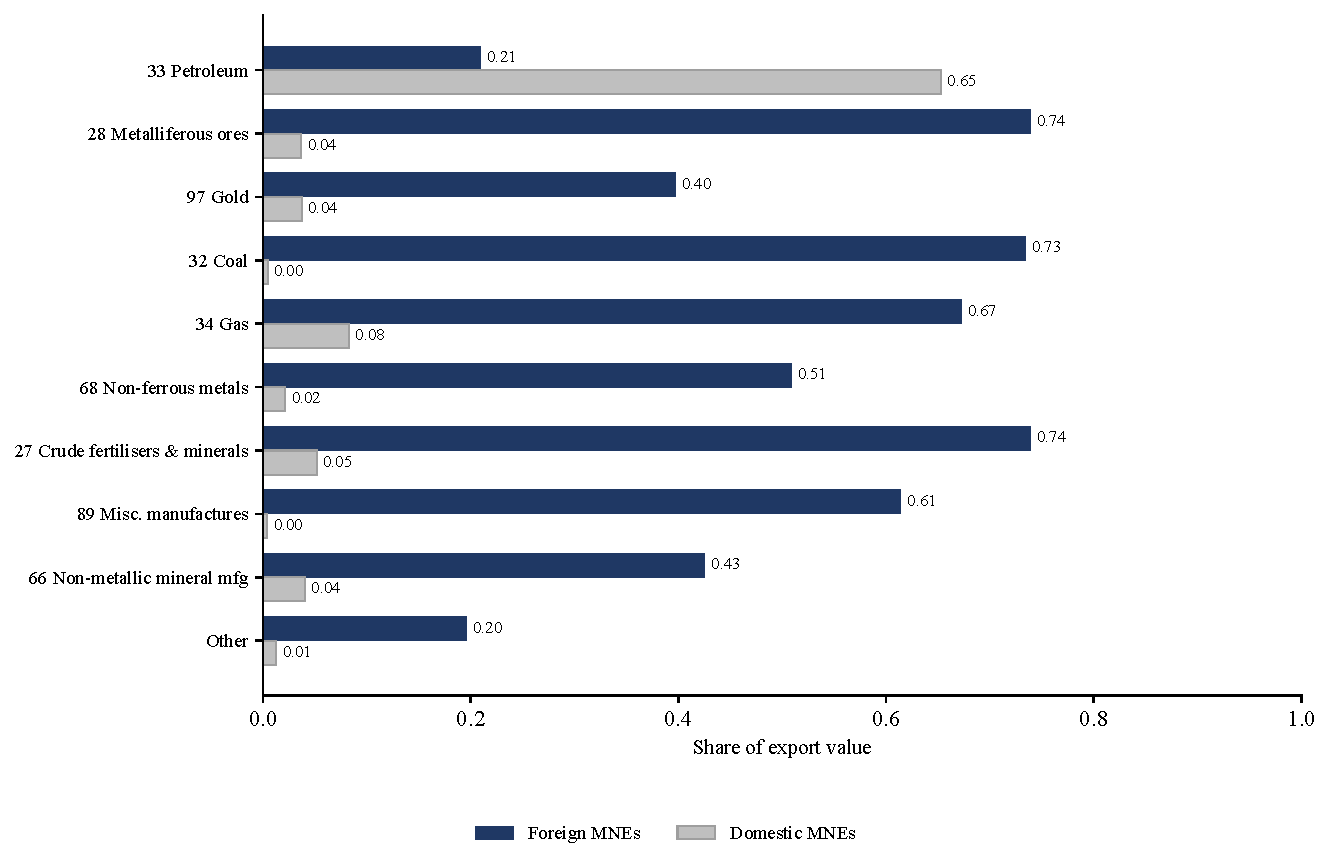
\includegraphics[width=0.9\textwidth,height=0.8\textheight,keepaspectratio]{figures/mining/fig_wp2_sitc2.pdf}%
  \caption{Mining and Fuels: Multinational Share of Export Value, by SITC Division}%
  \label{fig:sc_sitc2_f_mining}%
  \par\vspace{2pt}%
  \parbox{0.92\textwidth}{\footnotesize %
  \textit{Notes:} Shares of mining and fuels export value (HS 25--27 and 71), all available years pooled. SITC Rev.\,3 divisions; HS6 products without an SITC correspondence are excluded.\\[3pt]%
  \textit{Source:} Authors' calculations based on customs data matched to Orbis and Dun \& Bradstreet.}%
  \end{figure}
% ---- Figure: Mining and Fuels: Foreign-Multinational Share of Export Value, by Exporting Country and SITC Division
\begin{figure}[H]\centering%
  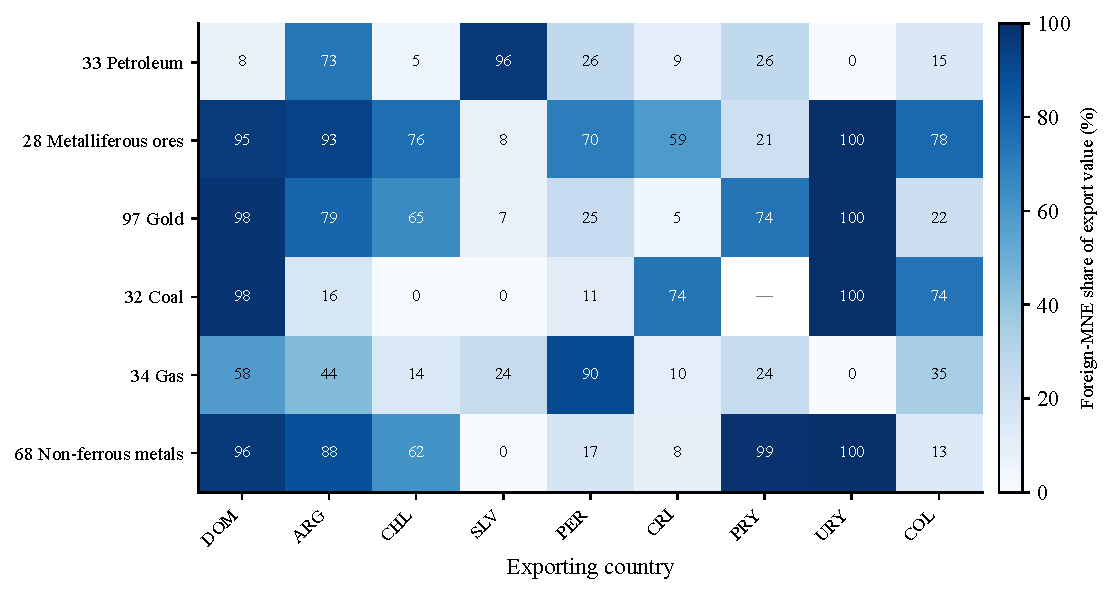
\includegraphics[width=0.95\textwidth,height=0.8\textheight,keepaspectratio]{figures/mining/fig_wp2_origin_x_sitc2.pdf}%
  \caption{Mining and Fuels: Foreign-Multinational Share of Export Value, by Exporting Country and SITC Division}%
  \label{fig:sc_sitc2_hm_mining}%
  \par\vspace{2pt}%
  \parbox{0.92\textwidth}{\footnotesize %
  \textit{Notes:} Percent of each group's export value in each country shipped by foreign MNEs. SITC Rev.\,3 divisions; HS6 products without an SITC correspondence are excluded.\\[3pt]%
  \textit{Source:} Authors' calculations based on customs data matched to Orbis and Dun \& Bradstreet.}%
  \end{figure}
% ---- Table: Mining and Fuels: Exports by Exporting Country and SITC Division
\begin{table}[H]\centering\footnotesize%
  \caption{Mining and Fuels: Exports by Exporting Country and SITC Division}%
  \label{tab:sc_sitc2_ht_mining}%
  \adjustbox{max width=\textwidth, max totalheight=0.8\textheight}{\begin{tabular}{lrrrrrrrrrr}
\toprule
Sub-sector & ARG & CHL & COL & CRI & DOM & PER & PRY & SLV & URY & All \\
\midrule
\multicolumn{11}{l}{\textit{Panel A: composition of the origin's exports, \% (columns sum to 100)}} \\
33 Petroleum & 35.4 & 1.1 & 67.3 & 11.9 & 4.9 & 11.0 & 58.1 & 55.3 & 19.0 & 34.1 \\
28 Metalliferous ores & 16.5 & 90.5 & 0.2 & 5.6 & 4.1 & 52.5 & 0.0 & 0.3 & 0.5 & 33.9 \\
97 Gold & 32.6 & 5.1 & 7.9 & 25.5 & 67.6 & 29.6 & 31.1 & 22.5 & 34.1 & 17.4 \\
32 Coal & 0.1 & 0.1 & 23.0 & 0.1 & 0.0 & 0.1 & 0.0 & 0.0 & 0.0 & 9.4 \\
34 Gas & 9.4 & 0.3 & 0.6 & 0.2 & 0.2 & 3.7 & 5.0 & 0.2 & 0.5 & 2.2 \\
68 Non-ferrous metals & 4.0 & 2.0 & 0.2 & 1.5 & 1.0 & 1.2 & 0.1 & 0.2 & 0.0 & 1.1 \\
27 Crude fertilisers \& minerals & 0.8 & 0.8 & 0.1 & 5.4 & 0.3 & 1.3 & 4.9 & 5.4 & 1.2 & 0.7 \\
89 Misc. manufactures & 0.0 & 0.0 & 0.1 & 15.5 & 17.2 & 0.4 & 0.8 & 2.1 & 0.5 & 0.5 \\
66 Non-metallic mineral mfg & 0.8 & 0.0 & 0.5 & 34.3 & 4.7 & 0.1 & 0.0 & 7.4 & 21.3 & 0.5 \\
Other & 0.3 & 0.0 & 0.2 & 0.0 & 0.0 & 0.0 & 0.0 & 6.6 & 22.9 & 0.2 \\
All sub-sectors & 100.0 & 100.0 & 100.0 & 100.0 & 100.0 & 100.0 & 100.0 & 100.0 & 100.0 & 100.0 \\
\midrule
\multicolumn{11}{l}{\textit{Panel B: foreign-MNE share of export value, \%}} \\
33 Petroleum & 73.0 & 5.0 & 15.2 & 9.4 & 7.8 & 26.2 & 26.3 & 95.9 & 0.2 & 21.0 \\
28 Metalliferous ores & 92.9 & 76.1 & 78.1 & 58.6 & 95.4 & 70.2 & 21.5 & 7.6 & 100.0 & 73.9 \\
97 Gold & 79.4 & 64.9 & 21.7 & 4.6 & 98.4 & 24.8 & 73.8 & 6.9 & 100.0 & 39.7 \\
32 Coal & 16.4 & 0.0 & 73.8 & 73.7 & 98.0 & 11.3 & -- & 0.0 & 100.0 & 73.4 \\
34 Gas & 44.1 & 14.2 & 34.5 & 9.9 & 58.1 & 89.6 & 24.4 & 24.2 & 0.0 & 67.2 \\
68 Non-ferrous metals & 87.7 & 61.8 & 13.3 & 8.1 & 96.1 & 17.1 & 98.6 & 0.1 & 100.0 & 50.9 \\
27 Crude fertilisers \& minerals & 31.5 & 64.8 & 17.3 & 62.9 & 37.0 & 90.3 & 77.9 & 76.4 & 44.9 & 73.9 \\
89 Misc. manufactures & 11.9 & 24.5 & 67.8 & 44.7 & 57.9 & 75.5 & 94.8 & 0.4 & 69.2 & 61.4 \\
66 Non-metallic mineral mfg & 21.5 & 28.6 & 26.2 & 97.6 & 71.2 & 58.5 & 0.0 & 0.0 & 34.4 & 42.6 \\
Other & 23.5 & 25.9 & 32.8 & 99.9 & 97.2 & 12.8 & 100.0 & 1.7 & 0.1 & 19.6 \\
All sub-sectors & 75.3 & 74.1 & 29.6 & 49.6 & 85.3 & 52.2 & 44.1 & 58.9 & 42.9 & 49.2 \\
\bottomrule
\end{tabular}
}%
  \par\vspace{3pt}%
  \begin{minipage}{0.95\textwidth}\footnotesize %
  \textit{Notes:} Panel A: composition of each country's exports in the sector (rows add to 100). Panel B: percent of each cell's export value shipped by foreign MNEs. SITC Rev.\,3 divisions; HS6 products without an SITC correspondence are excluded.\\[3pt]%
  \textit{Source:} Authors' calculations based on customs data matched to Orbis and Dun \& Bradstreet.%
  \end{minipage}%
  \end{table}
% ---- Table: Mining and Fuels: Exports by SITC Division and Parent Country
\begin{table}[H]\centering\footnotesize%
  \caption{Mining and Fuels: Exports by SITC Division and Parent Country}%
  \label{tab:sc_sitc2_par_mining}%
  \adjustbox{max width=\textwidth, max totalheight=0.8\textheight}{\begin{tabular}{lrrrrrrrrrrrr}
\toprule
SITC Rev.\,3 division & GBR & USA & CAN & LIE & ESP & PAN & AUS & BRA & BGR & FRA & Other & Domestic \\
\midrule
33 Petroleum & 0.5 & 7.8 & 1.3 & 0.4 & 4.3 & 0.1 & 0.0 & 0.5 & 1.9 & 0.3 & 4.0 & 65.3 \\
28 Metalliferous ores & 39.8 & 7.0 & 5.9 & 9.5 & 0.2 & 2.7 & 3.2 & 0.6 & 0.0 & 0.7 & 4.2 & 3.7 \\
97 Gold & 0.7 & 3.2 & 26.0 & 0.0 & 0.3 & 1.3 & 0.5 & 0.4 & 0.1 & 0.1 & 7.0 & 3.7 \\
32 Coal & 34.0 & 33.4 & 0.7 & 0.0 & 0.1 & 0.8 & 0.0 & 0.0 & 0.2 & 0.3 & 4.0 & 0.5 \\
34 Gas & 1.6 & 52.8 & 0.0 & 0.0 & 0.8 & 0.0 & 0.0 & 0.0 & 0.0 & 8.1 & 3.9 & 8.3 \\
68 Non-ferrous metals & 10.7 & 0.2 & 29.9 & 0.0 & 0.0 & 0.2 & 0.9 & 0.0 & 0.0 & 0.7 & 8.2 & 2.2 \\
27 Crude fertilisers \& minerals & 0.1 & 0.8 & 0.3 & 0.0 & 0.1 & 1.1 & 0.8 & 50.4 & 0.0 & 0.1 & 20.2 & 5.2 \\
89 Misc. manufactures & 6.1 & 13.3 & 0.0 & 0.0 & 2.1 & 2.6 & 0.0 & 0.1 & 0.0 & 13.3 & 23.7 & 0.4 \\
66 Non-metallic mineral mfg & 0.8 & 0.1 & 0.1 & 0.0 & 3.4 & 1.2 & 0.0 & 2.0 & 4.1 & 0.0 & 30.9 & 4.1 \\
Other & 0.0 & 0.6 & 16.0 & 0.0 & 0.0 & 0.0 & 0.0 & 0.0 & 0.0 & 0.0 & 3.0 & 1.3 \\
\bottomrule
\end{tabular}
}%
  \par\vspace{3pt}%
  \begin{minipage}{0.95\textwidth}\footnotesize %
  \textit{Notes:} Percent of each group's export value, by country of the ultimate parent of foreign MNEs; domestic MNEs shown for comparison. SITC Rev.\,3 divisions; HS6 products without an SITC correspondence are excluded.\\[3pt]%
  \textit{Source:} Authors' calculations based on customs data matched to Orbis and Dun \& Bradstreet.%
  \end{minipage}%
  \end{table}

\subsection{By NAICS Industry}
% ---- Table: Mining and Fuels: Exports and Multinational Shares, by NAICS Industry
\begin{table}[H]\centering\footnotesize%
  \caption{Mining and Fuels: Exports and Multinational Shares, by NAICS Industry}%
  \label{tab:sc_naics3_mining}%
  \adjustbox{max width=\textwidth, max totalheight=0.8\textheight}{\begin{tabular}{@{}l r r r r l@{}}
\toprule
NAICS 3-digit (product-based) & Total exports (US\$bn/yr) & MNE exports (US\$bn/yr) & Foreign (\%) & Domestic (\%) & Leading parents (share of foreign) \\
\midrule
212 Mining (excl. oil \& gas) & 29.7 & 22.9 & 74.9 & 3.0 & GBR 0.53, USA 0.18, LIE 0.10 \\
211 Oil \& gas extraction & 19.6 & 18.4 & 24.8 & 69.7 & USA 0.52, ESP 0.17, BGR 0.09 \\
331 Primary metals & 15.0 & 6.8 & 40.3 & 3.7 & CAN 0.69, USA 0.08, PAN 0.03 \\
324 Petroleum \& coal products & 3.8 & 2.6 & 20.4 & 49.0 & ESP 0.52, USA 0.17, BRA 0.13 \\
339 Misc. manufacturing & 0.6 & 0.3 & 51.0 & 1.0 & USA 0.20, FRA 0.19, BEL 0.18 \\
Other & 0.8 & 0.3 & 34.9 & 2.5 & MEX 0.18, ESP 0.13, USA 0.10 \\
\midrule
All & 69.5 & 51.4 & 50.0 & 25.0 & \\
\bottomrule
\end{tabular}
}%
  \par\vspace{3pt}%
  \begin{minipage}{0.95\textwidth}\footnotesize %
  \textit{Notes:} NAICS 3-digit industries assigned to HS6 products. Foreign and domestic: percent of the group's export value. Leading parents: the three largest parent countries and their share of the row's foreign-MNE exports. Values are annual averages in US\$ billion.\\[3pt]%
  \textit{Source:} Authors' calculations based on customs data matched to Orbis and Dun \& Bradstreet.%
  \end{minipage}%
  \end{table}
% ---- Figure: Mining and Fuels: Multinational Share of Export Value, by NAICS Industry
\begin{figure}[H]\centering%
  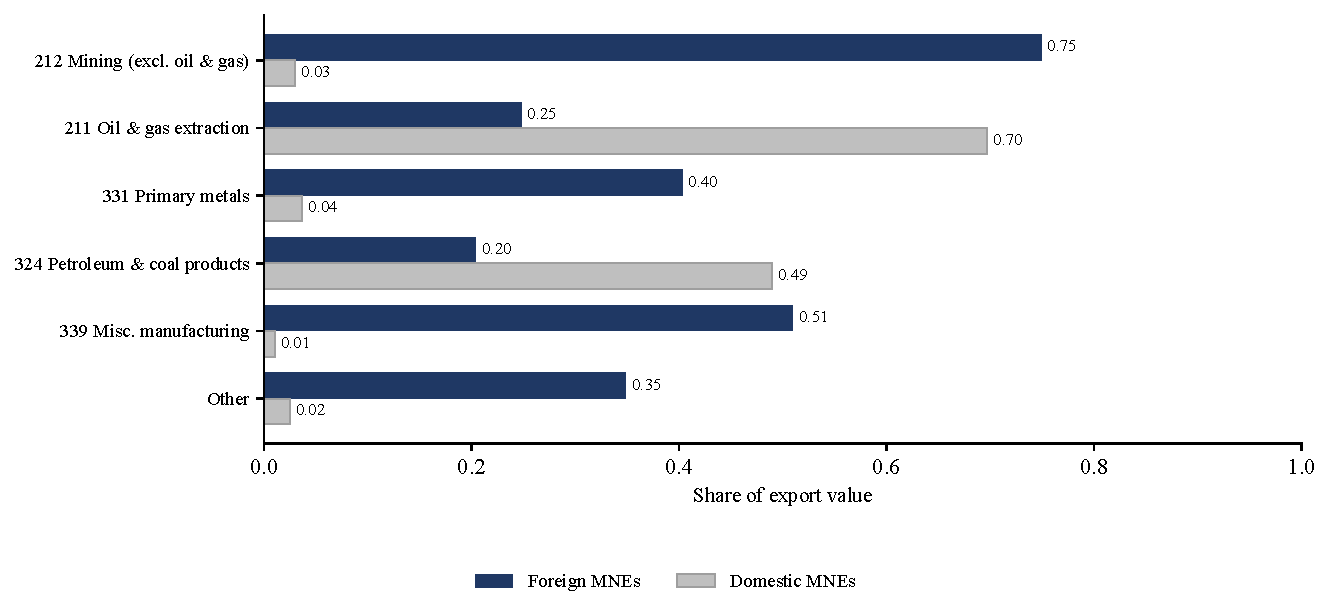
\includegraphics[width=0.9\textwidth,height=0.8\textheight,keepaspectratio]{figures/mining/fig_wp2_naics3.pdf}%
  \caption{Mining and Fuels: Multinational Share of Export Value, by NAICS Industry}%
  \label{fig:sc_naics3_f_mining}%
  \par\vspace{2pt}%
  \parbox{0.92\textwidth}{\footnotesize %
  \textit{Notes:} Shares of mining and fuels export value (HS 25--27 and 71), all available years pooled. NAICS 3-digit industries assigned to HS6 products.\\[3pt]%
  \textit{Source:} Authors' calculations based on customs data matched to Orbis and Dun \& Bradstreet.}%
  \end{figure}
% ---- Figure: Mining and Fuels: Foreign-Multinational Share of Export Value, by Exporting Country and NAICS Industry
\begin{figure}[H]\centering%
  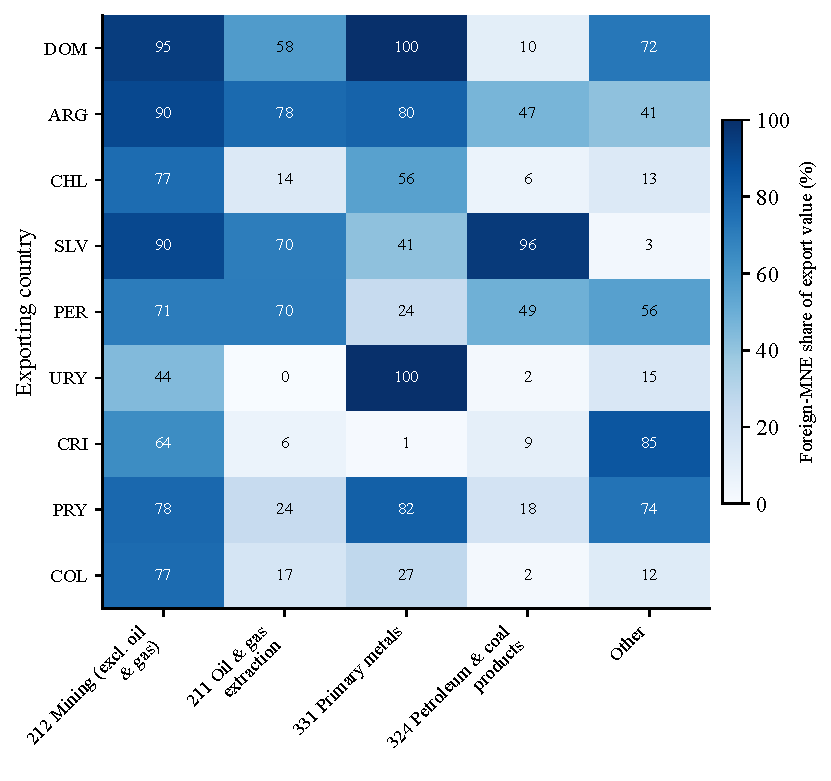
\includegraphics[width=0.95\textwidth,height=0.8\textheight,keepaspectratio]{figures/mining/fig_wp2_origin_x_naics3.pdf}%
  \caption{Mining and Fuels: Foreign-Multinational Share of Export Value, by Exporting Country and NAICS Industry}%
  \label{fig:sc_naics3_hm_mining}%
  \par\vspace{2pt}%
  \parbox{0.92\textwidth}{\footnotesize %
  \textit{Notes:} Percent of each group's export value in each country shipped by foreign MNEs. NAICS 3-digit industries assigned to HS6 products.\\[3pt]%
  \textit{Source:} Authors' calculations based on customs data matched to Orbis and Dun \& Bradstreet.}%
  \end{figure}
% ---- Table: Mining and Fuels: Exports by Exporting Country and NAICS Industry
\begin{table}[H]\centering\footnotesize%
  \caption{Mining and Fuels: Exports by Exporting Country and NAICS Industry}%
  \label{tab:sc_naics3_ht_mining}%
  \adjustbox{max width=\textwidth, max totalheight=0.8\textheight}{\begin{tabular}{lrrrrrrr}
\toprule
Origin & 212 Mining (excl. oil \& gas) & 211 Oil \& gas extraction & 331 Primary metals & 324 Petroleum \& coal products & 339 Misc. manufacturing & Other & All \\
\midrule
\multicolumn{8}{l}{\textit{Panel A: composition of the origin's exports, \% (rows sum to 100)}} \\
ARG & 18.8 & 34.7 & 40.5 & 4.1 & 0.1 & 1.9 & 100.0 \\
CHL & 90.4 & 0.3 & 8.2 & 0.9 & 0.0 & 0.2 & 100.0 \\
COL & 21.3 & 60.0 & 9.7 & 7.7 & 0.6 & 0.9 & 100.0 \\
CRI & 5.2 & 0.2 & 21.9 & 11.8 & 16.4 & 44.5 & 100.0 \\
DOM & 4.3 & 0.3 & 67.9 & 0.1 & 18.1 & 9.4 & 100.0 \\
PER & 56.6 & 5.2 & 32.5 & 5.1 & 0.4 & 0.3 & 100.0 \\
PRY & 5.3 & 5.6 & 1.9 & 53.7 & 0.1 & 33.4 & 100.0 \\
SLV & 4.6 & 0.6 & 1.7 & 54.5 & 2.4 & 36.2 & 100.0 \\
URY & 1.4 & 0.6 & 41.4 & 2.8 & 13.9 & 40.0 & 100.0 \\
All origins & 44.1 & 29.0 & 19.7 & 5.4 & 0.8 & 1.0 & 100.0 \\
\midrule
\multicolumn{8}{l}{\textit{Panel B: foreign-MNE share of export value, \%}} \\
ARG & 90.4 & 77.6 & 80.2 & 46.6 & 12.6 & 41.4 & 79.0 \\
CHL & 76.9 & 13.5 & 55.8 & 6.1 & 6.8 & 13.4 & 74.2 \\
COL & 77.1 & 16.9 & 26.7 & 1.9 & 35.0 & 12.1 & 29.5 \\
CRI & 64.1 & 5.9 & 1.0 & 8.8 & 42.6 & 85.4 & 49.6 \\
DOM & 94.9 & 58.1 & 99.7 & 9.9 & 57.9 & 72.4 & 89.2 \\
PER & 70.7 & 70.4 & 24.4 & 48.9 & 76.1 & 56.0 & 54.5 \\
PRY & 78.5 & 24.4 & 81.6 & 18.0 & 13.9 & 73.9 & 41.4 \\
SLV & 90.4 & 70.0 & 41.4 & 95.9 & 0.3 & 2.7 & 58.5 \\
URY & 44.5 & 0.0 & 100.0 & 1.7 & 24.4 & 15.2 & 51.5 \\
All origins & 74.9 & 24.8 & 40.3 & 20.4 & 51.0 & 34.9 & 50.0 \\
\bottomrule
\end{tabular}
}%
  \par\vspace{3pt}%
  \begin{minipage}{0.95\textwidth}\footnotesize %
  \textit{Notes:} Panel A: composition of each country's exports in the sector (rows add to 100). Panel B: percent of each cell's export value shipped by foreign MNEs. NAICS 3-digit industries assigned to HS6 products.\\[3pt]%
  \textit{Source:} Authors' calculations based on customs data matched to Orbis and Dun \& Bradstreet.%
  \end{minipage}%
  \end{table}
% ---- Table: Mining and Fuels: Exports by NAICS Industry and Parent Country
\begin{table}[H]\centering\footnotesize%
  \caption{Mining and Fuels: Exports by NAICS Industry and Parent Country}%
  \label{tab:sc_naics3_par_mining}%
  \adjustbox{max width=\textwidth, max totalheight=0.8\textheight}{\begin{tabular}{lrrrrrrrrrrrr}
\toprule
NAICS 3-digit (product-based) & GBR & USA & CAN & LIE & ESP & PAN & AUS & BRA & BGR & FRA & Other & Domestic \\
\midrule
212 Mining (excl. oil \& gas) & 39.0 & 12.9 & 4.8 & 7.5 & 0.1 & 2.3 & 2.5 & 1.3 & 0.0 & 0.6 & 3.8 & 3.0 \\
211 Oil \& gas extraction & 0.3 & 12.8 & 1.6 & 0.4 & 4.1 & 0.0 & 0.0 & 0.0 & 2.2 & 0.7 & 2.6 & 69.7 \\
331 Primary metals & 1.3 & 2.9 & 25.3 & 0.0 & 0.1 & 1.3 & 0.5 & 0.4 & 0.0 & 0.1 & 8.5 & 3.7 \\
324 Petroleum \& coal products & 0.5 & 2.0 & 0.0 & 0.0 & 6.1 & 0.7 & 0.0 & 1.5 & 0.0 & 0.1 & 9.6 & 49.0 \\
339 Misc. manufacturing & 4.9 & 9.4 & 0.1 & 0.0 & 3.5 & 1.8 & 0.0 & 0.1 & 2.8 & 9.3 & 19.2 & 1.0 \\
Other & 0.2 & 3.5 & 3.1 & 0.0 & 4.5 & 2.4 & 0.0 & 2.0 & 1.8 & 1.3 & 16.0 & 2.5 \\
\bottomrule
\end{tabular}
}%
  \par\vspace{3pt}%
  \begin{minipage}{0.95\textwidth}\footnotesize %
  \textit{Notes:} Percent of each group's export value, by country of the ultimate parent of foreign MNEs; domestic MNEs shown for comparison. NAICS 3-digit industries assigned to HS6 products.\\[3pt]%
  \textit{Source:} Authors' calculations based on customs data matched to Orbis and Dun \& Bradstreet.%
  \end{minipage}%
  \end{table}

\subsection{By Technology Class}
% ---- Table: Mining and Fuels: Exports and Multinational Shares, by Technology Class
\begin{table}[H]\centering\footnotesize%
  \caption{Mining and Fuels: Exports and Multinational Shares, by Technology Class}%
  \label{tab:sc_lall2000_category_mining}%
  \adjustbox{max width=\textwidth, max totalheight=0.8\textheight}{\begin{tabular}{@{}l r r r r l@{}}
\toprule
Lall (2000) category & Total exports (US\$bn/yr) & MNE exports (US\$bn/yr) & Foreign (\%) & Domestic (\%) & Leading parents (share of foreign) \\
\midrule
Resource-based manufactures: other & 30.6 & 21.7 & 62.9 & 9.3 & GBR 0.53, LIE 0.13, USA 0.10 \\
Primary products & 26.7 & 23.7 & 38.0 & 51.2 & USA 0.47, GBR 0.23, ESP 0.08 \\
Unclassified products & 13.9 & 6.2 & 39.5 & 3.7 & CAN 0.69, USA 0.09, CYM 0.04 \\
Low technology manufactures: other products & 0.5 & 0.3 & 61.4 & 0.4 & FRA 0.22, USA 0.22, BEL 0.21 \\
\midrule
All & 71.7 & 51.9 & 49.2 & 24.5 & \\
\bottomrule
\end{tabular}
}%
  \par\vspace{3pt}%
  \begin{minipage}{0.95\textwidth}\footnotesize %
  \textit{Notes:} Lall (2000) technology classes. Foreign and domestic: percent of the group's export value. Leading parents: the three largest parent countries and their share of the row's foreign-MNE exports. Values are annual averages in US\$ billion.\\[3pt]%
  \textit{Source:} Authors' calculations based on customs data matched to Orbis and Dun \& Bradstreet.%
  \end{minipage}%
  \end{table}
% ---- Figure: Mining and Fuels: Multinational Share of Export Value, by Technology Class
\begin{figure}[H]\centering%
  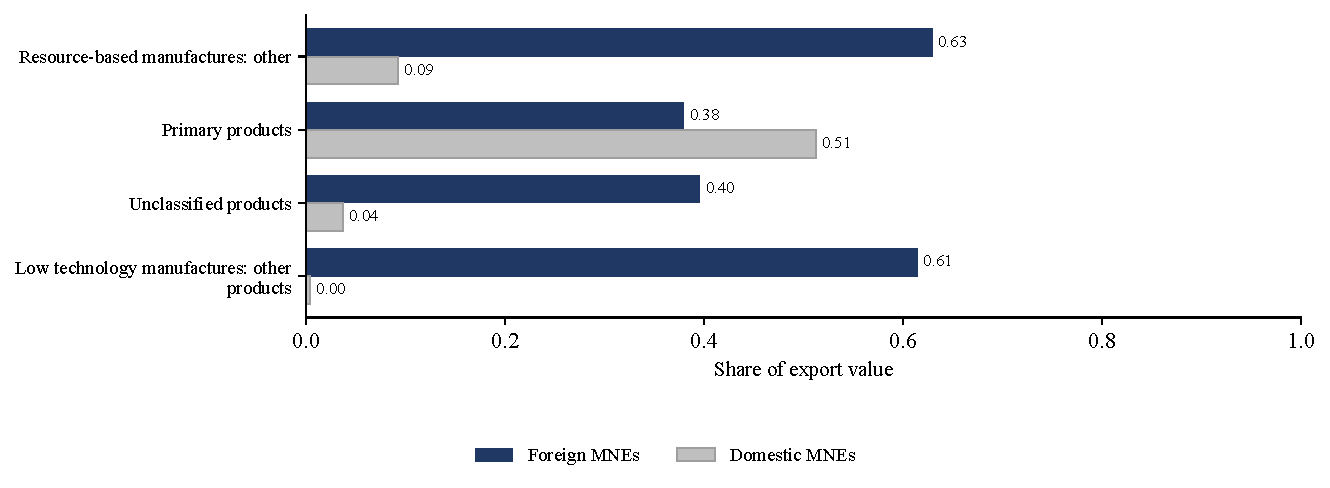
\includegraphics[width=0.9\textwidth,height=0.8\textheight,keepaspectratio]{figures/mining/fig_wp2_lall2000_category.pdf}%
  \caption{Mining and Fuels: Multinational Share of Export Value, by Technology Class}%
  \label{fig:sc_lall2000_category_f_mining}%
  \par\vspace{2pt}%
  \parbox{0.92\textwidth}{\footnotesize %
  \textit{Notes:} Shares of mining and fuels export value (HS 25--27 and 71), all available years pooled. Lall (2000) technology classes.\\[3pt]%
  \textit{Source:} Authors' calculations based on customs data matched to Orbis and Dun \& Bradstreet.}%
  \end{figure}
% ---- Figure: Mining and Fuels: Foreign-Multinational Share of Export Value, by Exporting Country and Technology Class
\begin{figure}[H]\centering%
  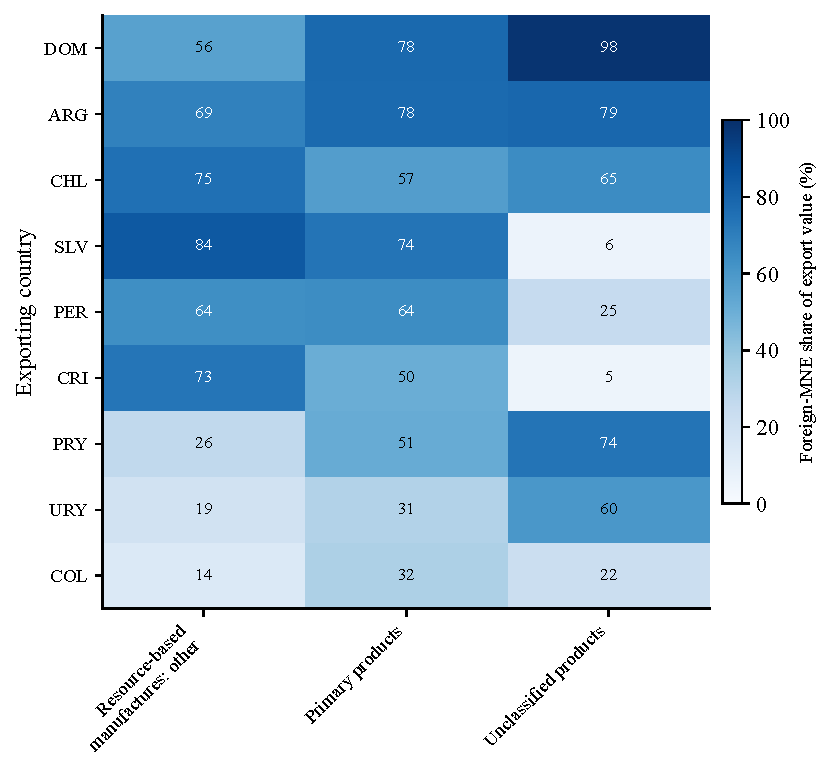
\includegraphics[width=0.95\textwidth,height=0.8\textheight,keepaspectratio]{figures/mining/fig_wp2_origin_x_lall2000_category.pdf}%
  \caption{Mining and Fuels: Foreign-Multinational Share of Export Value, by Exporting Country and Technology Class}%
  \label{fig:sc_lall2000_category_hm_mining}%
  \par\vspace{2pt}%
  \parbox{0.92\textwidth}{\footnotesize %
  \textit{Notes:} Percent of each group's export value in each country shipped by foreign MNEs. Lall (2000) technology classes.\\[3pt]%
  \textit{Source:} Authors' calculations based on customs data matched to Orbis and Dun \& Bradstreet.}%
  \end{figure}
% ---- Table: Mining and Fuels: Exports by Exporting Country and Technology Class
\begin{table}[H]\centering\footnotesize%
  \caption{Mining and Fuels: Exports by Exporting Country and Technology Class}%
  \label{tab:sc_lall2000_category_ht_mining}%
  \adjustbox{max width=\textwidth, max totalheight=0.8\textheight}{\begin{tabular}{lrrrrr}
\toprule
Origin & Resource-based manufactures: other & Primary products & Unclassified products & Low technology manufactures: other products & All \\
\midrule
\multicolumn{6}{l}{\textit{Panel A: composition of the origin's exports, \% (rows sum to 100)}} \\
ARG & 30.8 & 36.3 & 32.8 & 0.0 & 100.0 \\
CHL & 91.7 & 3.1 & 5.1 & 0.0 & 100.0 \\
COL & 11.1 & 80.7 & 8.1 & 0.1 & 100.0 \\
CRI & 51.9 & 7.1 & 25.6 & 15.5 & 100.0 \\
DOM & 13.6 & 1.6 & 67.6 & 17.2 & 100.0 \\
PER & 62.4 & 7.6 & 29.6 & 0.4 & 100.0 \\
PRY & 58.1 & 10.0 & 31.1 & 0.8 & 100.0 \\
SLV & 62.6 & 6.2 & 29.1 & 2.1 & 100.0 \\
URY & 40.8 & 1.7 & 57.0 & 0.5 & 100.0 \\
All origins & 43.3 & 38.6 & 17.5 & 0.5 & 100.0 \\
\midrule
\multicolumn{6}{l}{\textit{Panel B: foreign-MNE share of export value, \%}} \\
ARG & 68.7 & 77.6 & 78.9 & 11.9 & 75.3 \\
CHL & 75.2 & 57.1 & 64.7 & 24.5 & 74.1 \\
COL & 13.9 & 32.5 & 22.0 & 67.8 & 29.6 \\
CRI & 73.1 & 50.1 & 4.8 & 44.7 & 49.6 \\
DOM & 55.7 & 78.0 & 98.4 & 57.9 & 85.3 \\
PER & 63.6 & 64.3 & 24.8 & 75.5 & 52.2 \\
PRY & 26.3 & 51.2 & 73.8 & 94.8 & 44.1 \\
SLV & 84.2 & 73.7 & 5.7 & 0.4 & 58.9 \\
URY & 19.3 & 31.2 & 59.9 & 69.2 & 42.9 \\
All origins & 62.9 & 38.0 & 39.5 & 61.4 & 49.2 \\
\bottomrule
\end{tabular}
}%
  \par\vspace{3pt}%
  \begin{minipage}{0.95\textwidth}\footnotesize %
  \textit{Notes:} Panel A: composition of each country's exports in the sector (rows add to 100). Panel B: percent of each cell's export value shipped by foreign MNEs. Lall (2000) technology classes.\\[3pt]%
  \textit{Source:} Authors' calculations based on customs data matched to Orbis and Dun \& Bradstreet.%
  \end{minipage}%
  \end{table}
% ---- Table: Mining and Fuels: Exports by Technology Class and Parent Country
\begin{table}[H]\centering\footnotesize%
  \caption{Mining and Fuels: Exports by Technology Class and Parent Country}%
  \label{tab:sc_lall2000_category_par_mining}%
  \adjustbox{max width=\textwidth, max totalheight=0.8\textheight}{\begin{tabular}{lrrrrrrrrrrrr}
\toprule
Lall (2000) category & GBR & USA & CAN & LIE & ESP & PAN & AUS & BRA & BGR & FRA & Other & Domestic \\
\midrule
Resource-based manufactures: other & 31.5 & 5.9 & 4.6 & 7.4 & 1.0 & 2.3 & 2.5 & 0.9 & 0.0 & 0.7 & 6.0 & 9.3 \\
Primary products & 8.8 & 17.6 & 2.2 & 0.3 & 3.0 & 0.1 & 0.0 & 0.9 & 1.7 & 0.6 & 2.7 & 51.2 \\
Unclassified products & 0.7 & 3.2 & 25.9 & 0.0 & 0.3 & 1.3 & 0.5 & 0.4 & 0.1 & 0.1 & 7.0 & 3.7 \\
Low technology manufactures: other products & 6.1 & 13.3 & 0.0 & 0.0 & 2.1 & 2.6 & 0.0 & 0.1 & 0.0 & 13.3 & 23.7 & 0.4 \\
\bottomrule
\end{tabular}
}%
  \par\vspace{3pt}%
  \begin{minipage}{0.95\textwidth}\footnotesize %
  \textit{Notes:} Percent of each group's export value, by country of the ultimate parent of foreign MNEs; domestic MNEs shown for comparison. Lall (2000) technology classes.\\[3pt]%
  \textit{Source:} Authors' calculations based on customs data matched to Orbis and Dun \& Bradstreet.%
  \end{minipage}%
  \end{table}

\subsection{HS Section and End Use}
% ---- Table: Mining and Fuels: Exports by HS Section and End Use
\begin{table}[H]\centering\small%
  \caption{Mining and Fuels: Exports by HS Section and End Use}%
  \label{tab:sxe_v_mining}%
  \adjustbox{max width=\textwidth, max totalheight=0.8\textheight}{\begin{tabular}{lrrrr}
\toprule
HS section / BEC end use & Intermediate & Consumption & Capital & Total \\
\midrule
V Mineral products & 50.6 & 0.0 & 0.0 & 50.6 \\
XIV Precious metals and stones & 14.8 & 0.5 & 0.0 & 15.3 \\
\midrule
Total & 65.4 & 0.5 & 0.0 & 65.9 \\
\bottomrule
\end{tabular}
}%
  \par\vspace{3pt}%
  \begin{minipage}{0.95\textwidth}\footnotesize %
  \textit{Notes:} Export value by HS section and BEC Rev.\,4 end use. Values are annual averages in US\$ billion.\\[3pt]%
  \textit{Source:} Authors' calculations based on customs data matched to Orbis and Dun \& Bradstreet.%
  \end{minipage}%
  \end{table}
% ---- Table: Mining and Fuels: Foreign-Multinational Share of Exports by HS Section and End Use
\begin{table}[H]\centering\small%
  \caption{Mining and Fuels: Foreign-Multinational Share of Exports by HS Section and End Use}%
  \label{tab:sxe_f_mining}%
  \adjustbox{max width=\textwidth, max totalheight=0.8\textheight}{\begin{tabular}{lrrr}
\toprule
HS section / BEC end use & Intermediate & Consumption & Capital \\
\midrule
V Mineral products & 54.5 & -- & -- \\
XIV Precious metals and stones & 40.2 & 61.7 & 21.4 \\
\bottomrule
\end{tabular}
}%
  \par\vspace{3pt}%
  \begin{minipage}{0.95\textwidth}\footnotesize %
  \textit{Notes:} Percent of each cell's export value shipped by foreign MNEs.\\[3pt]%
  \textit{Source:} Authors' calculations based on customs data matched to Orbis and Dun \& Bradstreet.%
  \end{minipage}%
  \end{table}
\clearpage\part{Other Goods}

\section{Fact 1: Multinationals Account for a Large Share of Exports}\label{sec:f1_rest}
% ---- Figure: Other Goods: Multinational Share of Export Value, by Exporting Country
\begin{figure}[H]\centering%
  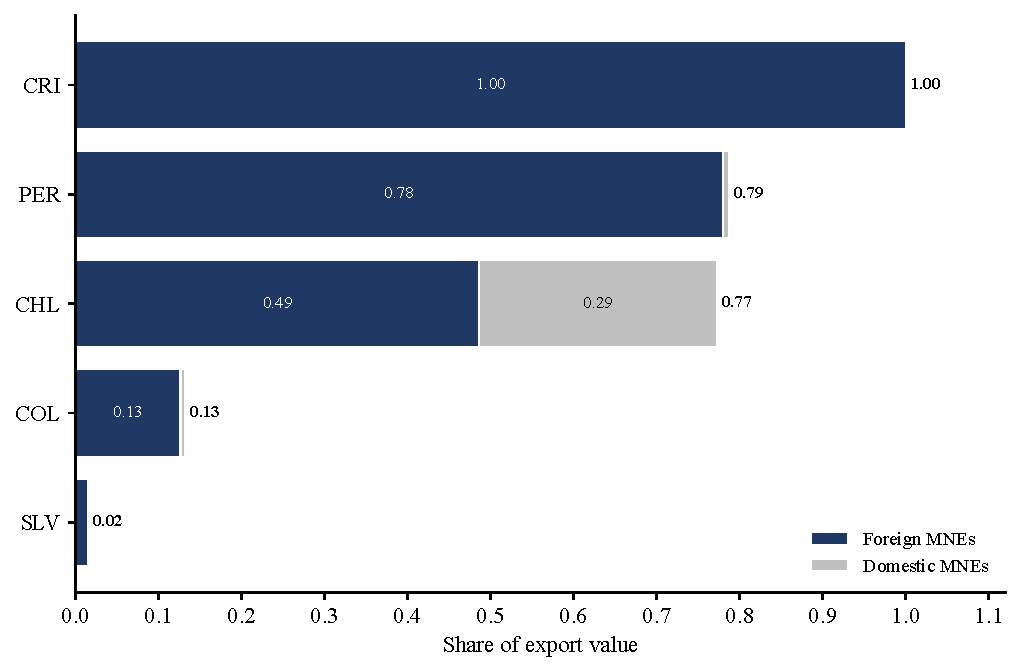
\includegraphics[width=0.8\textwidth,height=0.8\textheight,keepaspectratio]{figures/rest/fig_wp0_fig1_origin.pdf}%
  \caption{Other Goods: Multinational Share of Export Value, by Exporting Country}%
  \label{fig:f1_rest}%
  \par\vspace{2pt}%
  \parbox{0.92\textwidth}{\footnotesize %
  \textit{Notes:} Shares of export value of other goods (HS 98--99 and unclassified codes), all available years pooled. The figure at the end of each bar is the total MNE share.\\[3pt]%
  \textit{Source:} Authors' calculations based on customs data matched to Orbis and Dun \& Bradstreet.}%
  \end{figure}
% ---- Table: Other Goods: Multinational Share of Export Value, by Exporting Country
\begin{table}[H]\centering\small%
  \caption{Other Goods: Multinational Share of Export Value, by Exporting Country}%
  \label{tab:f1n_rest}%
  \adjustbox{max width=\textwidth, max totalheight=0.8\textheight}{\begin{tabular}{lrrrr}
\toprule
Origin & Foreign & Domestic & All MNEs & Value (US\$bn/yr) \\
\midrule
CRI & 1.000 & 0.000 & 1.000 & 0.0 \\
PER & 0.780 & 0.008 & 0.787 & 0.0 \\
CHL & 0.486 & 0.286 & 0.772 & 0.5 \\
COL & 0.127 & 0.006 & 0.133 & 0.0 \\
SLV & 0.015 & 0.000 & 0.015 & 0.0 \\
\midrule
All & 0.479 & 0.280 & 0.759 & 0.5 \\
\bottomrule
\end{tabular}
}%
  \par\vspace{3pt}%
  \begin{minipage}{0.95\textwidth}\footnotesize %
  \textit{Notes:} Shares of export value of other goods (HS 98--99 and unclassified codes), all available years pooled. Values are annual averages in US\$ billion.\\[3pt]%
  \textit{Source:} Authors' calculations based on customs data matched to Orbis and Dun \& Bradstreet.%
  \end{minipage}%
  \end{table}

\subsection{By Parent Country}
% ---- Figure: Other Goods: Multinational Share of Export Value, by Exporting Country and Parent Country
\begin{figure}[H]\centering%
  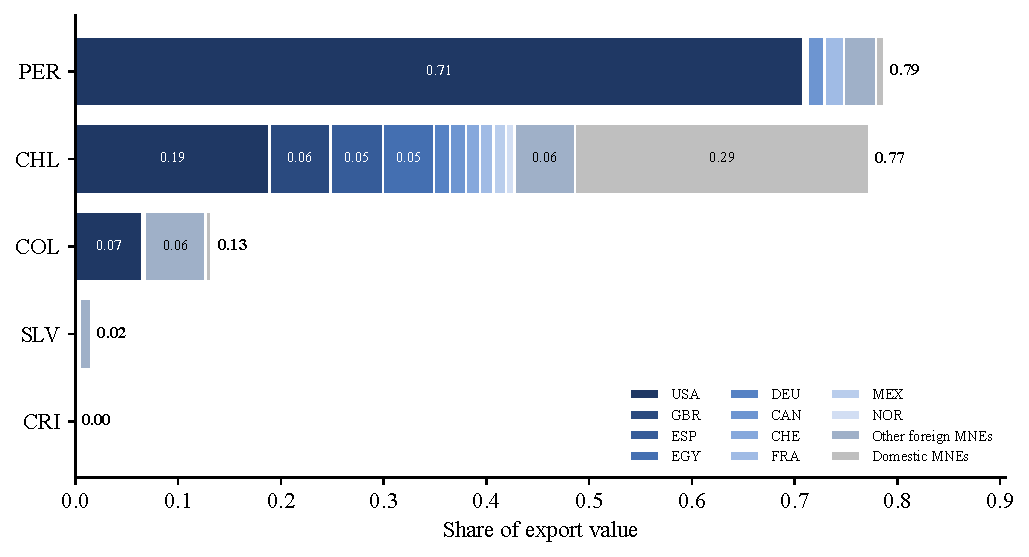
\includegraphics[width=0.92\textwidth,height=0.8\textheight,keepaspectratio]{figures/rest/fig_wp1a_origin_by_parent.pdf}%
  \caption{Other Goods: Multinational Share of Export Value, by Exporting Country and Parent Country}%
  \label{fig:f1p_rest}%
  \par\vspace{2pt}%
  \parbox{0.92\textwidth}{\footnotesize %
  \textit{Notes:} Shares of export value of other goods (HS 98--99 and unclassified codes), all available years pooled. Foreign MNEs split by country of the ultimate parent; the ten largest parent countries are shown separately.\\[3pt]%
  \textit{Source:} Authors' calculations based on customs data matched to Orbis and Dun \& Bradstreet.}%
  \end{figure}
% ---- Table: Other Goods: Multinational Share of Export Value, by Exporting Country and Parent Country
\begin{table}[H]\centering\small%
  \caption{Other Goods: Multinational Share of Export Value, by Exporting Country and Parent Country}%
  \label{tab:f1pn_rest}%
  \adjustbox{max width=\textwidth, max totalheight=0.8\textheight}{\begin{tabular}{lcccccccccccccc}
\toprule
Origin & USA & GBR & ESP & EGY & DEU & CAN & CHE & FRA & MEX & NOR & Other & Domestic & All MNEs & Value (US\$bn/yr) \\
\midrule
PER & 0.708 & 0.002 & 0.000 & 0.000 & 0.002 & 0.016 & 0.000 & 0.019 & 0.000 & 0.000 & 0.032 & 0.008 & 0.787 & 0.0 \\
CHL & 0.189 & 0.059 & 0.052 & 0.049 & 0.016 & 0.016 & 0.013 & 0.013 & 0.012 & 0.008 & 0.059 & 0.286 & 0.772 & 0.5 \\
COL & 0.065 & 0.001 & 0.001 & 0.000 & 0.000 & 0.000 & 0.000 & 0.001 & 0.000 & 0.000 & 0.059 & 0.006 & 0.133 & 0.0 \\
SLV & 0.000 & 0.001 & 0.002 & 0.000 & 0.001 & 0.000 & 0.000 & 0.000 & 0.001 & 0.000 & 0.011 & 0.000 & 0.015 & 0.0 \\
CRI & 0.000 & 0.000 & 0.000 & 0.000 & 0.000 & 0.000 & 0.000 & 0.000 & 0.000 & 0.000 & 0.000 & 0.000 & 0.000 & 0.0 \\
\bottomrule
\end{tabular}
}%
  \par\vspace{3pt}%
  \begin{minipage}{0.95\textwidth}\footnotesize %
  \textit{Notes:} Shares of export value of other goods (HS 98--99 and unclassified codes), all available years pooled. Other: all remaining foreign parents. Values are annual averages in US\$ billion.\\[3pt]%
  \textit{Source:} Authors' calculations based on customs data matched to Orbis and Dun \& Bradstreet.%
  \end{minipage}%
  \end{table}

\section{Fact 2: Foreign Multinationals Specialize in Complex Products, Domestic Multinationals in Primary Goods}\label{sec:f2_rest}
Product characteristics (complexity, technology class, elasticities) are not available for
these codes, so this fact cannot be computed for them.


\section{Fact 3: Multinationals from a Small Set of Countries Dominate Exports}\label{sec:f3_rest}

\subsection{Parent Countries}
% ---- Figure: Other Goods: Foreign-Multinational Exports, by Parent Country
\begin{figure}[H]\centering%
  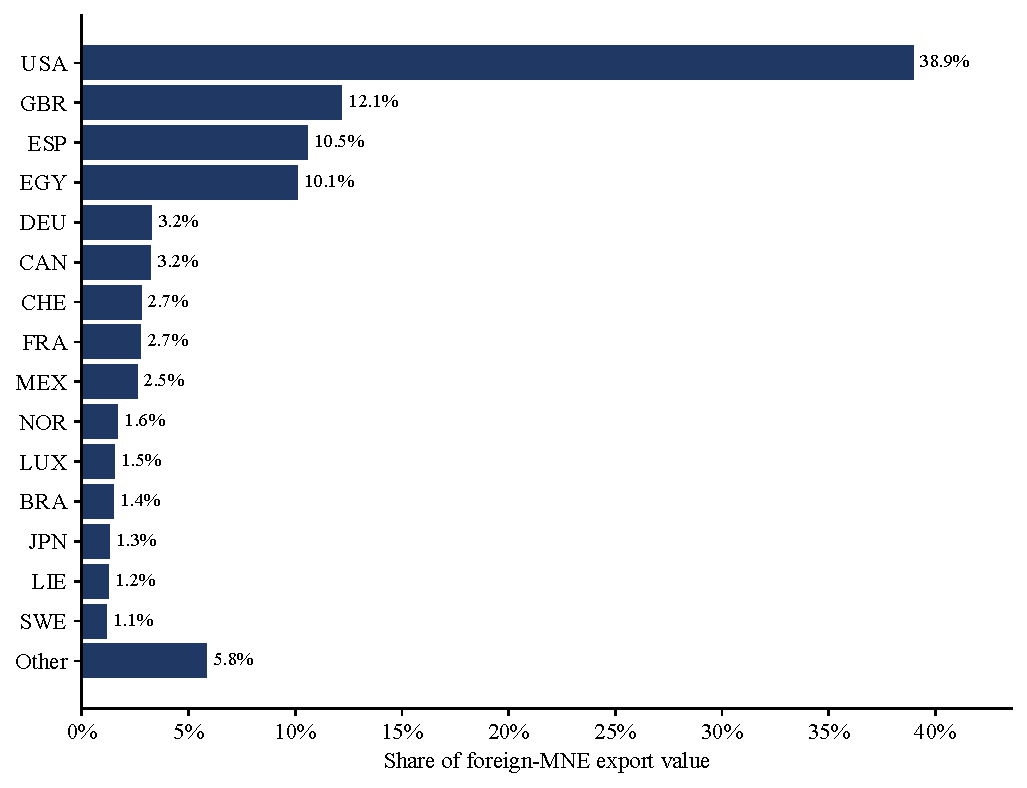
\includegraphics[width=0.78\textwidth,height=0.8\textheight,keepaspectratio]{figures/rest/fig_wp1a_parent_share.pdf}%
  \caption{Other Goods: Foreign-Multinational Exports, by Parent Country}%
  \label{fig:f4_rest}%
  \par\vspace{2pt}%
  \parbox{0.92\textwidth}{\footnotesize %
  \textit{Notes:} Percent of foreign-MNE export value, by country of the ultimate parent.\\[3pt]%
  \textit{Source:} Authors' calculations based on customs data matched to Orbis and Dun \& Bradstreet.}%
  \end{figure}
% ---- Table: Other Goods: Foreign-Multinational Exports, by Parent Country
\begin{table}[H]\centering\small%
  \caption{Other Goods: Foreign-Multinational Exports, by Parent Country}%
  \label{tab:f4n_rest}%
  \adjustbox{max width=\textwidth, max totalheight=0.8\textheight}{\begin{tabular}{lrr}
\toprule
Parent country & Share (\%) & Value (US\$bn/yr) \\
\midrule
USA & 38.9 & 0.1 \\
GBR & 12.1 & 0.0 \\
ESP & 10.5 & 0.0 \\
EGY & 10.1 & 0.0 \\
DEU & 3.2 & 0.0 \\
CAN & 3.2 & 0.0 \\
CHE & 2.7 & 0.0 \\
FRA & 2.7 & 0.0 \\
MEX & 2.5 & 0.0 \\
NOR & 1.6 & 0.0 \\
LUX & 1.5 & 0.0 \\
BRA & 1.4 & 0.0 \\
JPN & 1.3 & 0.0 \\
LIE & 1.2 & 0.0 \\
SWE & 1.1 & 0.0 \\
Other (64 countries) & 5.8 & 0.0 \\
\midrule
All foreign MNEs & 100.0 & 0.2 \\
\bottomrule
\end{tabular}
}%
  \par\vspace{3pt}%
  \begin{minipage}{0.95\textwidth}\footnotesize %
  \textit{Notes:} Percent of foreign-MNE export value, by country of the ultimate parent. Values are annual averages in US\$ billion.\\[3pt]%
  \textit{Source:} Authors' calculations based on customs data matched to Orbis and Dun \& Bradstreet.%
  \end{minipage}%
  \end{table}
% ---- Figure: Other Goods: Share of Total Exports, by Parent Country
\begin{figure}[H]\centering%
  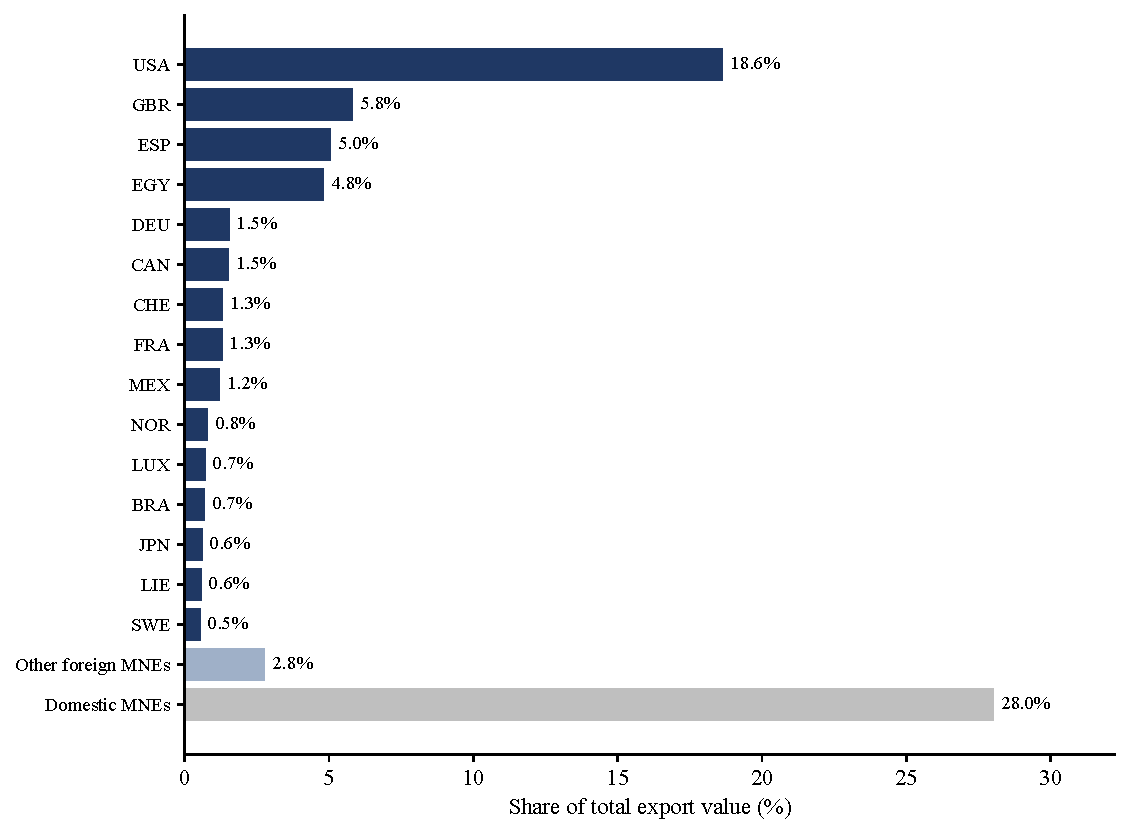
\includegraphics[width=0.85\textwidth,height=0.8\textheight,keepaspectratio]{figures/rest/fig_wp1a_parent_share_total.pdf}%
  \caption{Other Goods: Share of Total Exports, by Parent Country}%
  \label{fig:f4t_rest}%
  \par\vspace{2pt}%
  \parbox{0.92\textwidth}{\footnotesize %
  \textit{Notes:} Percent of total export value shipped by foreign MNEs of each parent country, other foreign MNEs and domestic MNEs; the remainder is local firms.\\[3pt]%
  \textit{Source:} Authors' calculations based on customs data matched to Orbis and Dun \& Bradstreet.}%
  \end{figure}
% ---- Table: Other Goods: Share of Total Exports, by Parent Country
\begin{table}[H]\centering\small%
  \caption{Other Goods: Share of Total Exports, by Parent Country}%
  \label{tab:f4tn_rest}%
  \adjustbox{max width=\textwidth, max totalheight=0.8\textheight}{\begin{tabular}{lr}
\toprule
Exporter type / parent country & Share of total exports (\%) \\
\midrule
USA & 18.6 \\
GBR & 5.8 \\
ESP & 5.0 \\
EGY & 4.8 \\
DEU & 1.5 \\
CAN & 1.5 \\
CHE & 1.3 \\
FRA & 1.3 \\
MEX & 1.2 \\
NOR & 0.8 \\
LUX & 0.7 \\
BRA & 0.7 \\
JPN & 0.6 \\
LIE & 0.6 \\
SWE & 0.5 \\
Other foreign MNEs & 2.8 \\
Domestic MNEs & 28.0 \\
\midrule
All MNEs & 75.9 \\
Local firms & 24.1 \\
\bottomrule
\end{tabular}
}%
  \par\vspace{3pt}%
  \begin{minipage}{0.95\textwidth}\footnotesize %
  \textit{Notes:} Percent of total export value, by type of exporter and parent country.\\[3pt]%
  \textit{Source:} Authors' calculations based on customs data matched to Orbis and Dun \& Bradstreet.%
  \end{minipage}%
  \end{table}

\subsection{Parent Region and Destination Region}
% ---- Table: Other Goods: Multinational Exports by Parent Region and Destination Region: Export Value
\begin{table}[H]\centering\small%
  \caption{Other Goods: Multinational Exports by Parent Region and Destination Region: Export Value}%
  \label{tab:reg_value_rest}%
  \adjustbox{max width=\textwidth, max totalheight=0.8\textheight}{\begin{tabular}{lrrrrrrrr}
\toprule
Parent region / Destination region & Latin America & North America & Europe & Asia & Africa & Oceania & Rest of World & Total \\
\midrule
Latin America & 0.0 & 0.0 & 0.0 & 0.0 & 0.0 & 0.0 & 0.0 & 0.0 \\
North America & 0.0 & 0.0 & 0.0 & 0.0 & 0.0 & 0.0 & 0.0 & 0.1 \\
Europe & 0.0 & 0.0 & 0.0 & 0.0 & 0.0 & 0.0 & 0.0 & 0.1 \\
Asia & 0.0 & 0.0 & 0.0 & 0.0 & 0.0 & 0.0 & 0.0 & 0.0 \\
Africa & 0.0 & 0.0 & 0.0 & 0.0 & 0.0 & 0.0 & 0.0 & 0.0 \\
Oceania & 0.0 & 0.0 & 0.0 & 0.0 & 0.0 & 0.0 & 0.0 & 0.0 \\
Rest of World & 0.0 & 0.0 & 0.0 & 0.0 & 0.0 & 0.0 & 0.0 & 0.0 \\
Domestic MNEs & 0.1 & 0.0 & 0.0 & 0.0 & 0.0 & 0.0 & 0.0 & 0.1 \\
Local firms & 0.1 & 0.0 & 0.0 & 0.0 & 0.0 & 0.0 & 0.0 & 0.1 \\
\midrule
Total & 0.3 & 0.1 & 0.1 & 0.0 & 0.0 & 0.0 & 0.0 & 0.4 \\
\bottomrule
\end{tabular}
}%
  \par\vspace{3pt}%
  \begin{minipage}{0.95\textwidth}\footnotesize %
  \textit{Notes:} Values are annual averages in US\$ billion. Rows: region of the ultimate parent; columns: destination region.\\[3pt]%
  \textit{Source:} Authors' calculations based on customs data matched to Orbis and Dun \& Bradstreet.%
  \end{minipage}%
  \end{table}
% ---- Table: Other Goods: Multinational Exports by Parent Region and Destination Region: Row Percentages
\begin{table}[H]\centering\small%
  \caption{Other Goods: Multinational Exports by Parent Region and Destination Region: Row Percentages}%
  \label{tab:reg_rowpct_rest}%
  \adjustbox{max width=\textwidth, max totalheight=0.8\textheight}{\begin{tabular}{lrrrrrrrr}
\toprule
Parent region / Destination region & Latin America & North America & Europe & Asia & Africa & Oceania & Rest of World & Total \\
\midrule
Latin America & 33.1 & 22.2 & 39.9 & 3.8 & 0.1 & 0.2 & 0.7 & 100.0 \\
North America & 51.8 & 39.0 & 7.8 & 1.3 & 0.0 & 0.1 & 0.0 & 100.0 \\
Europe & 30.2 & 37.1 & 30.1 & 2.0 & 0.2 & 0.4 & 0.0 & 100.0 \\
Asia & 30.0 & 17.7 & 13.0 & 39.1 & 0.0 & 0.1 & 0.0 & 100.0 \\
Africa & 82.7 & 2.7 & 10.8 & 2.7 & 0.7 & 0.0 & 0.4 & 100.0 \\
Oceania & 78.6 & 7.2 & 0.3 & 12.3 & 0.0 & 1.6 & 0.0 & 100.0 \\
Rest of World & 5.0 & 0.0 & 0.0 & 95.0 & 0.0 & 0.0 & 0.0 & 100.0 \\
Domestic MNEs & 92.6 & 4.0 & 3.0 & 0.4 & 0.0 & 0.0 & 0.0 & 100.0 \\
Local firms & 50.6 & 18.3 & 26.5 & 4.0 & 0.3 & 0.2 & 0.0 & 100.0 \\
\bottomrule
\end{tabular}
}%
  \par\vspace{3pt}%
  \begin{minipage}{0.95\textwidth}\footnotesize %
  \textit{Notes:} Percent of each group's exports, by destination region (rows add to 100). Domestic MNEs and local firms are shown for comparison.\\[3pt]%
  \textit{Source:} Authors' calculations based on customs data matched to Orbis and Dun \& Bradstreet.%
  \end{minipage}%
  \end{table}
% ---- Table: Other Goods: Multinational Exports by Parent Region and Destination Region: Column Percentages
\begin{table}[H]\centering\small%
  \caption{Other Goods: Multinational Exports by Parent Region and Destination Region: Column Percentages}%
  \label{tab:reg_colpct_rest}%
  \adjustbox{max width=\textwidth, max totalheight=0.8\textheight}{\begin{tabular}{lrrrrrrr}
\toprule
Parent region / Destination region & Latin America & North America & Europe & Asia & Africa & Oceania & Rest of World \\
\midrule
Latin America & 1.4 & 2.9 & 6.5 & 4.1 & 1.2 & 3.2 & 43.3 \\
North America & 15.2 & 34.8 & 8.8 & 9.9 & 4.6 & 6.0 & 0.0 \\
Europe & 8.3 & 30.8 & 31.6 & 14.1 & 16.9 & 41.5 & 2.7 \\
Asia & 0.4 & 0.7 & 0.7 & 13.2 & 0.0 & 0.7 & 0.0 \\
Africa & 5.9 & 0.6 & 2.9 & 4.8 & 20.0 & 0.5 & 42.9 \\
Oceania & 0.1 & 0.0 & 0.0 & 0.6 & 0.0 & 1.2 & 0.0 \\
Rest of World & 0.0 & 0.0 & 0.0 & 3.5 & 0.0 & 0.0 & 0.0 \\
Domestic MNEs & 46.7 & 6.2 & 5.7 & 5.0 & 0.6 & 7.4 & 0.6 \\
Local firms & 21.9 & 24.1 & 43.9 & 44.7 & 56.7 & 39.3 & 10.5 \\
\midrule
Total & 100.0 & 100.0 & 100.0 & 100.0 & 100.0 & 100.0 & 100.0 \\
\bottomrule
\end{tabular}
}%
  \par\vspace{3pt}%
  \begin{minipage}{0.95\textwidth}\footnotesize %
  \textit{Notes:} Percent of the exports reaching each destination region, by parent region (columns add to 100).\\[3pt]%
  \textit{Source:} Authors' calculations based on customs data matched to Orbis and Dun \& Bradstreet.%
  \end{minipage}%
  \end{table}
% ---- Figure: Other Goods: Multinational Exports by Parent Region and Destination Region
\begin{figure}[H]\centering%
  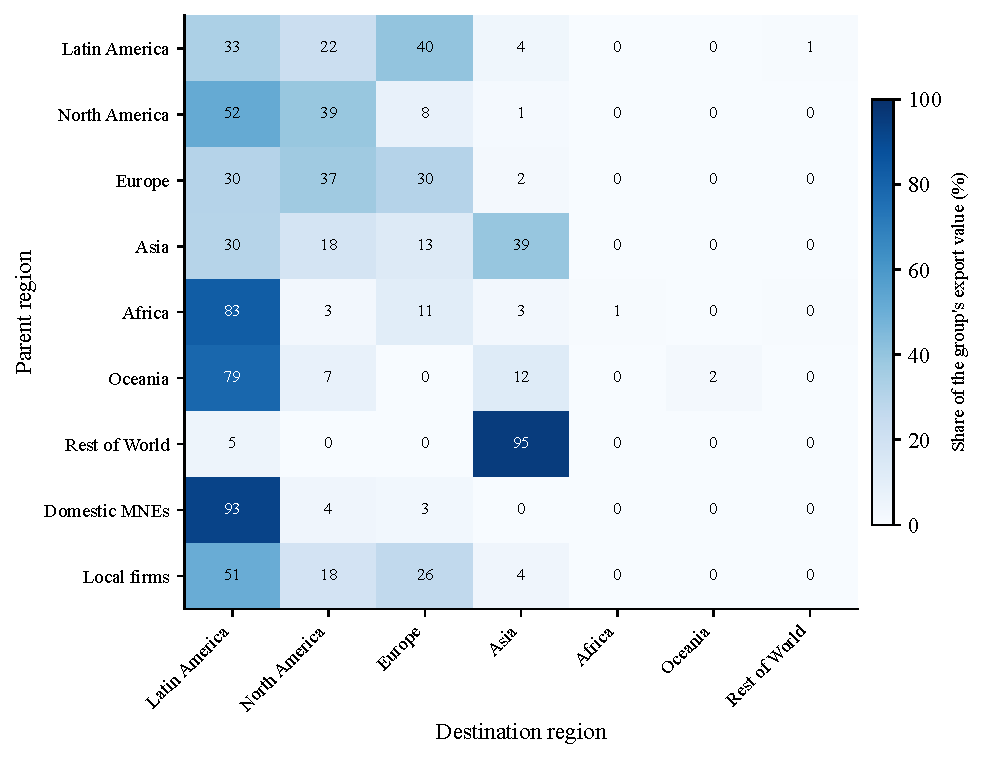
\includegraphics[width=0.9\textwidth,height=0.8\textheight,keepaspectratio]{figures/rest/fig_wp1d_heatmap_region_rowpct.pdf}%
  \caption{Other Goods: Multinational Exports by Parent Region and Destination Region}%
  \label{fig:reg_hm_rest}%
  \par\vspace{2pt}%
  \parbox{0.92\textwidth}{\footnotesize %
  \textit{Notes:} Percent of each group's exports, by destination region (rows add to 100).\\[3pt]%
  \textit{Source:} Authors' calculations based on customs data matched to Orbis and Dun \& Bradstreet.}%
  \end{figure}
% ---- Table: Other Goods: Foreign-Multinational Exports by Exporting Country and Destination Region
\begin{table}[H]\centering\small%
  \caption{Other Goods: Foreign-Multinational Exports by Exporting Country and Destination Region}%
  \label{tab:odr_f_rest}%
  \adjustbox{max width=\textwidth, max totalheight=0.8\textheight}{\begin{tabular}{lrrrrrrrr}
\toprule
Origin \ Destination region & Latin America & North America & Europe & Asia & Africa & Oceania & Rest of World & Total \\
\midrule
CHL & 37.3 & 42.1 & 17.3 & 2.9 & 0.1 & 0.2 & 0.1 & 0.2 \\
COL & 43.5 & 45.4 & 8.1 & 2.4 & 0.5 & 0.1 & 0.0 & 0.0 \\
CRI & 0.0 & 100.0 & 0.0 & 0.0 & 0.0 & 0.0 & 0.0 & 0.0 \\
PER & 12.9 & 85.6 & 0.5 & 1.0 & 0.0 & 0.0 & 0.0 & 0.0 \\
SLV & 65.5 & 13.1 & 14.6 & 2.9 & 3.8 & 0.0 & 0.0 & 0.0 \\
\bottomrule
\end{tabular}
}%
  \par\vspace{3pt}%
  \begin{minipage}{0.95\textwidth}\footnotesize %
  \textit{Notes:} Percent of each country's foreign-MNE exports, by destination region (rows add to 100). Last column: foreign-MNE exports. Values are annual averages in US\$ billion.\\[3pt]%
  \textit{Source:} Authors' calculations based on customs data matched to Orbis and Dun \& Bradstreet.%
  \end{minipage}%
  \end{table}
% ---- Table: Other Goods: Local-Firm Exports by Exporting Country and Destination Region
\begin{table}[H]\centering\small%
  \caption{Other Goods: Local-Firm Exports by Exporting Country and Destination Region}%
  \label{tab:odr_l_rest}%
  \adjustbox{max width=\textwidth, max totalheight=0.8\textheight}{\begin{tabular}{lrrrrrrrr}
\toprule
Origin \ Destination region & Latin America & North America & Europe & Asia & Africa & Oceania & Rest of World & Total \\
\midrule
CHL & 50.7 & 17.5 & 27.3 & 4.0 & 0.2 & 0.2 & 0.0 & 0.1 \\
COL & 48.1 & 28.0 & 16.8 & 4.9 & 1.4 & 0.7 & 0.0 & 0.0 \\
PER & 48.5 & 24.9 & 17.9 & 7.0 & 0.2 & 1.5 & 0.0 & 0.0 \\
SLV & 51.9 & 31.7 & 11.1 & 3.5 & 1.2 & 0.5 & 0.0 & 0.0 \\
\bottomrule
\end{tabular}
}%
  \par\vspace{3pt}%
  \begin{minipage}{0.95\textwidth}\footnotesize %
  \textit{Notes:} Percent of each country's exports by local firms, by destination region (rows add to 100). Last column: local-firm exports. Values are annual averages in US\$ billion.\\[3pt]%
  \textit{Source:} Authors' calculations based on customs data matched to Orbis and Dun \& Bradstreet.%
  \end{minipage}%
  \end{table}

\subsection{Parent Country and Destination Country}
% ---- Table: Other Goods: Foreign-Multinational Exports by Parent Country and Destination: Export Value
\begin{table}[H]\centering\small%
  \caption{Other Goods: Foreign-Multinational Exports by Parent Country and Destination: Export Value}%
  \label{tab:cty_value_rest}%
  \adjustbox{max width=\textwidth, max totalheight=0.8\textheight}{\begin{tabular}{lrrrrrrrrrrrr}
\toprule
Parent / Destination & USA & PER & ARG & ECU & GBR & ESP & CAN & MEX & DEU & COL & Other destinations & Total \\
\midrule
USA & 0.0 & 0.0 & 0.0 & 0.0 & 0.0 & 0.0 & 0.0 & 0.0 & 0.0 & 0.0 & 0.0 & 0.1 \\
GBR & 0.0 & 0.0 & 0.0 & 0.0 & 0.0 & 0.0 & 0.0 & 0.0 & 0.0 & 0.0 & 0.0 & 0.0 \\
ESP & 0.0 & 0.0 & 0.0 & 0.0 & 0.0 & 0.0 & 0.0 & 0.0 & 0.0 & 0.0 & 0.0 & 0.0 \\
EGY & 0.0 & 0.0 & 0.0 & 0.0 & 0.0 & 0.0 & 0.0 & 0.0 & 0.0 & 0.0 & 0.0 & 0.0 \\
DEU & 0.0 & 0.0 & 0.0 & 0.0 & 0.0 & 0.0 & 0.0 & 0.0 & 0.0 & 0.0 & 0.0 & 0.0 \\
CAN & 0.0 & 0.0 & 0.0 & 0.0 & 0.0 & 0.0 & 0.0 & 0.0 & 0.0 & 0.0 & 0.0 & 0.0 \\
CHE & 0.0 & 0.0 & 0.0 & 0.0 & 0.0 & 0.0 & 0.0 & 0.0 & 0.0 & 0.0 & 0.0 & 0.0 \\
FRA & 0.0 & 0.0 & 0.0 & 0.0 & 0.0 & 0.0 & 0.0 & 0.0 & 0.0 & 0.0 & 0.0 & 0.0 \\
MEX & 0.0 & 0.0 & 0.0 & 0.0 & 0.0 & 0.0 & 0.0 & 0.0 & 0.0 & 0.0 & 0.0 & 0.0 \\
NOR & 0.0 & 0.0 & 0.0 & 0.0 & 0.0 & 0.0 & 0.0 & 0.0 & 0.0 & 0.0 & 0.0 & 0.0 \\
Other parents & 0.0 & 0.0 & 0.0 & 0.0 & 0.0 & 0.0 & 0.0 & 0.0 & 0.0 & 0.0 & 0.0 & 0.0 \\
\midrule
Total & 0.1 & 0.0 & 0.0 & 0.0 & 0.0 & 0.0 & 0.0 & 0.0 & 0.0 & 0.0 & 0.0 & 0.2 \\
\bottomrule
\end{tabular}
}%
  \par\vspace{3pt}%
  \begin{minipage}{0.95\textwidth}\footnotesize %
  \textit{Notes:} Values are annual averages in US\$ billion. Ten largest parent countries and ten largest destinations by foreign-MNE export value.\\[3pt]%
  \textit{Source:} Authors' calculations based on customs data matched to Orbis and Dun \& Bradstreet.%
  \end{minipage}%
  \end{table}
% ---- Table: Other Goods: Foreign-Multinational Exports by Parent Country and Destination: Row Percentages
\begin{table}[H]\centering\small%
  \caption{Other Goods: Foreign-Multinational Exports by Parent Country and Destination: Row Percentages}%
  \label{tab:cty_rowpct_rest}%
  \adjustbox{max width=\textwidth, max totalheight=0.8\textheight}{\begin{tabular}{lrrrrrrrrrrrr}
\toprule
Parent / Destination & USA & PER & ARG & ECU & GBR & ESP & CAN & MEX & DEU & COL & Other destinations & Total \\
\midrule
USA & 39.3 & 32.8 & 10.0 & 0.5 & 1.5 & 1.5 & 2.3 & 1.0 & 0.6 & 1.0 & 9.5 & 100.0 \\
GBR & 66.4 & 9.6 & 1.6 & 0.5 & 10.7 & 0.0 & 1.0 & 1.0 & 0.2 & 3.0 & 6.2 & 100.0 \\
ESP & 14.1 & 3.9 & 8.2 & 0.7 & 5.0 & 24.6 & 3.1 & 9.4 & 1.4 & 3.4 & 26.3 & 100.0 \\
EGY & 2.6 & 4.8 & 4.9 & 66.1 & 2.5 & 0.3 & 0.0 & 0.2 & 2.1 & 0.0 & 16.6 & 100.0 \\
DEU & 33.2 & 2.8 & 1.4 & 0.3 & 0.0 & 0.0 & 5.9 & 0.5 & 51.2 & 0.8 & 4.0 & 100.0 \\
CAN & 0.8 & 27.8 & 26.6 & 0.9 & 0.0 & 18.2 & 7.2 & 0.2 & 1.2 & 11.8 & 5.3 & 100.0 \\
CHE & 9.8 & 16.6 & 4.7 & 2.9 & 2.0 & 0.3 & 24.6 & 6.0 & 0.3 & 3.6 & 29.1 & 100.0 \\
FRA & 17.9 & 2.5 & 14.7 & 1.0 & 0.0 & 0.6 & 1.4 & 1.5 & 0.3 & 2.3 & 57.9 & 100.0 \\
MEX & 13.1 & 2.1 & 7.0 & 0.3 & 60.4 & 0.7 & 7.8 & 3.8 & 0.4 & 0.1 & 4.3 & 100.0 \\
NOR & 1.3 & 9.2 & 30.9 & 3.3 & 0.0 & 0.4 & 0.0 & 19.3 & 3.3 & 13.8 & 18.5 & 100.0 \\
Other parents & 21.8 & 10.8 & 5.2 & 2.0 & 8.1 & 9.4 & 2.7 & 3.9 & 1.7 & 5.4 & 28.9 & 100.0 \\
\bottomrule
\end{tabular}
}%
  \par\vspace{3pt}%
  \begin{minipage}{0.95\textwidth}\footnotesize %
  \textit{Notes:} Percent of each parent country's exports, by destination (rows add to 100). Ten largest parent countries and destinations.\\[3pt]%
  \textit{Source:} Authors' calculations based on customs data matched to Orbis and Dun \& Bradstreet.%
  \end{minipage}%
  \end{table}
% ---- Table: Other Goods: Foreign-Multinational Exports by Parent Country and Destination: Column Percentages
\begin{table}[H]\centering\small%
  \caption{Other Goods: Foreign-Multinational Exports by Parent Country and Destination: Column Percentages}%
  \label{tab:cty_colpct_rest}%
  \adjustbox{max width=\textwidth, max totalheight=0.8\textheight}{\begin{tabular}{lrrrrrrrrrrr}
\toprule
Parent / Destination & USA & PER & ARG & ECU & GBR & ESP & CAN & MEX & DEU & COL & Other destinations \\
\midrule
USA & 51.0 & 71.5 & 47.6 & 2.5 & 11.3 & 11.8 & 29.6 & 14.3 & 9.7 & 15.7 & 23.8 \\
GBR & 26.9 & 6.5 & 2.3 & 0.8 & 24.6 & 0.0 & 3.9 & 4.5 & 0.8 & 14.2 & 4.8 \\
ESP & 4.9 & 2.3 & 10.5 & 1.0 & 10.1 & 51.8 & 10.8 & 37.7 & 5.8 & 13.8 & 17.8 \\
EGY & 0.9 & 2.7 & 6.0 & 89.5 & 4.8 & 0.6 & 0.0 & 0.8 & 8.0 & 0.0 & 10.8 \\
DEU & 3.6 & 0.5 & 0.5 & 0.1 & 0.0 & 0.0 & 6.3 & 0.6 & 63.2 & 1.0 & 0.8 \\
CAN & 0.1 & 5.0 & 10.4 & 0.4 & 0.0 & 11.6 & 7.8 & 0.3 & 1.5 & 14.5 & 1.1 \\
CHE & 0.9 & 2.5 & 1.6 & 1.1 & 1.0 & 0.2 & 22.5 & 6.2 & 0.3 & 3.8 & 5.1 \\
FRA & 1.6 & 0.4 & 4.9 & 0.4 & 0.0 & 0.3 & 1.2 & 1.5 & 0.3 & 2.5 & 10.1 \\
MEX & 1.1 & 0.3 & 2.2 & 0.1 & 29.3 & 0.4 & 6.7 & 3.7 & 0.3 & 0.1 & 0.7 \\
NOR & 0.1 & 0.8 & 6.2 & 0.7 & 0.0 & 0.1 & 0.0 & 12.1 & 2.1 & 8.7 & 2.0 \\
Other parents & 9.0 & 7.5 & 7.9 & 3.4 & 18.9 & 23.1 & 11.1 & 18.4 & 7.9 & 25.7 & 22.9 \\
\midrule
Total & 100.0 & 100.0 & 100.0 & 100.0 & 100.0 & 100.0 & 100.0 & 100.0 & 100.0 & 100.0 & 100.0 \\
\bottomrule
\end{tabular}
}%
  \par\vspace{3pt}%
  \begin{minipage}{0.95\textwidth}\footnotesize %
  \textit{Notes:} Percent of the foreign-MNE exports reaching each destination, by parent country (columns add to 100). Ten largest parent countries and destinations.\\[3pt]%
  \textit{Source:} Authors' calculations based on customs data matched to Orbis and Dun \& Bradstreet.%
  \end{minipage}%
  \end{table}
% ---- Figure: Other Goods: Destination of Foreign-Multinational Exports: Fifteen Largest Parent Countries and Destinations
\begin{figure}[H]\centering%
  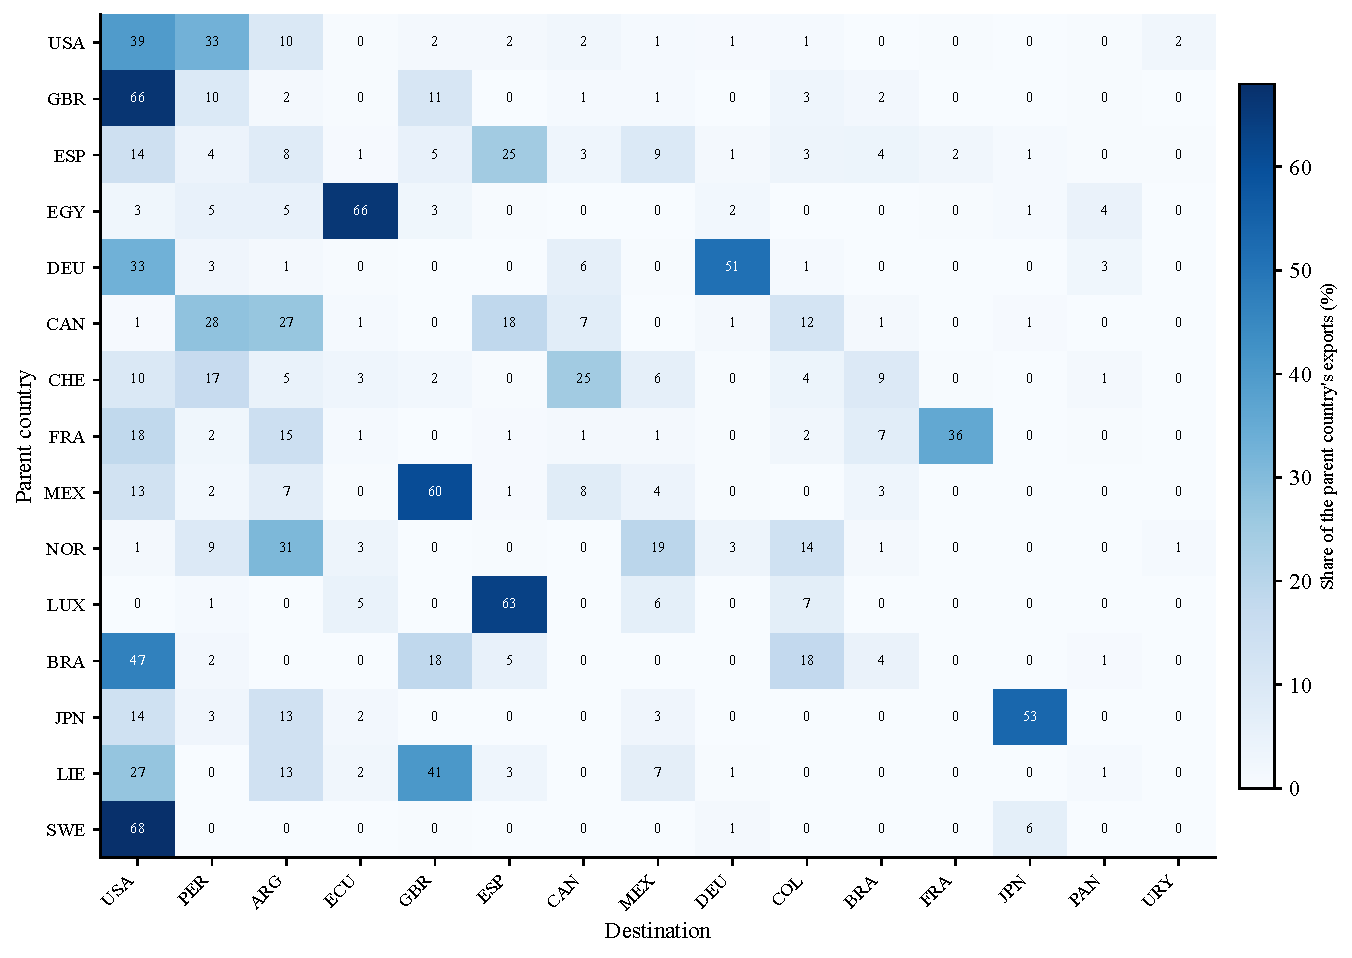
\includegraphics[width=1.0\textwidth,height=0.8\textheight,keepaspectratio]{figures/rest/fig_wp1d_heatmap_country_rowpct.pdf}%
  \caption{Other Goods: Destination of Foreign-Multinational Exports: Fifteen Largest Parent Countries and Destinations}%
  \label{fig:hm_row_rest}%
  \par\vspace{2pt}%
  \parbox{0.92\textwidth}{\footnotesize %
  \textit{Notes:} Percent of each parent country's exports going to each destination (rows add to 100 including other destinations).\\[3pt]%
  \textit{Source:} Authors' calculations based on customs data matched to Orbis and Dun \& Bradstreet.}%
  \end{figure}
% ---- Figure: Other Goods: Foreign-Multinational Exports by Parent Country and Destination: Share of the Total
\begin{figure}[H]\centering%
  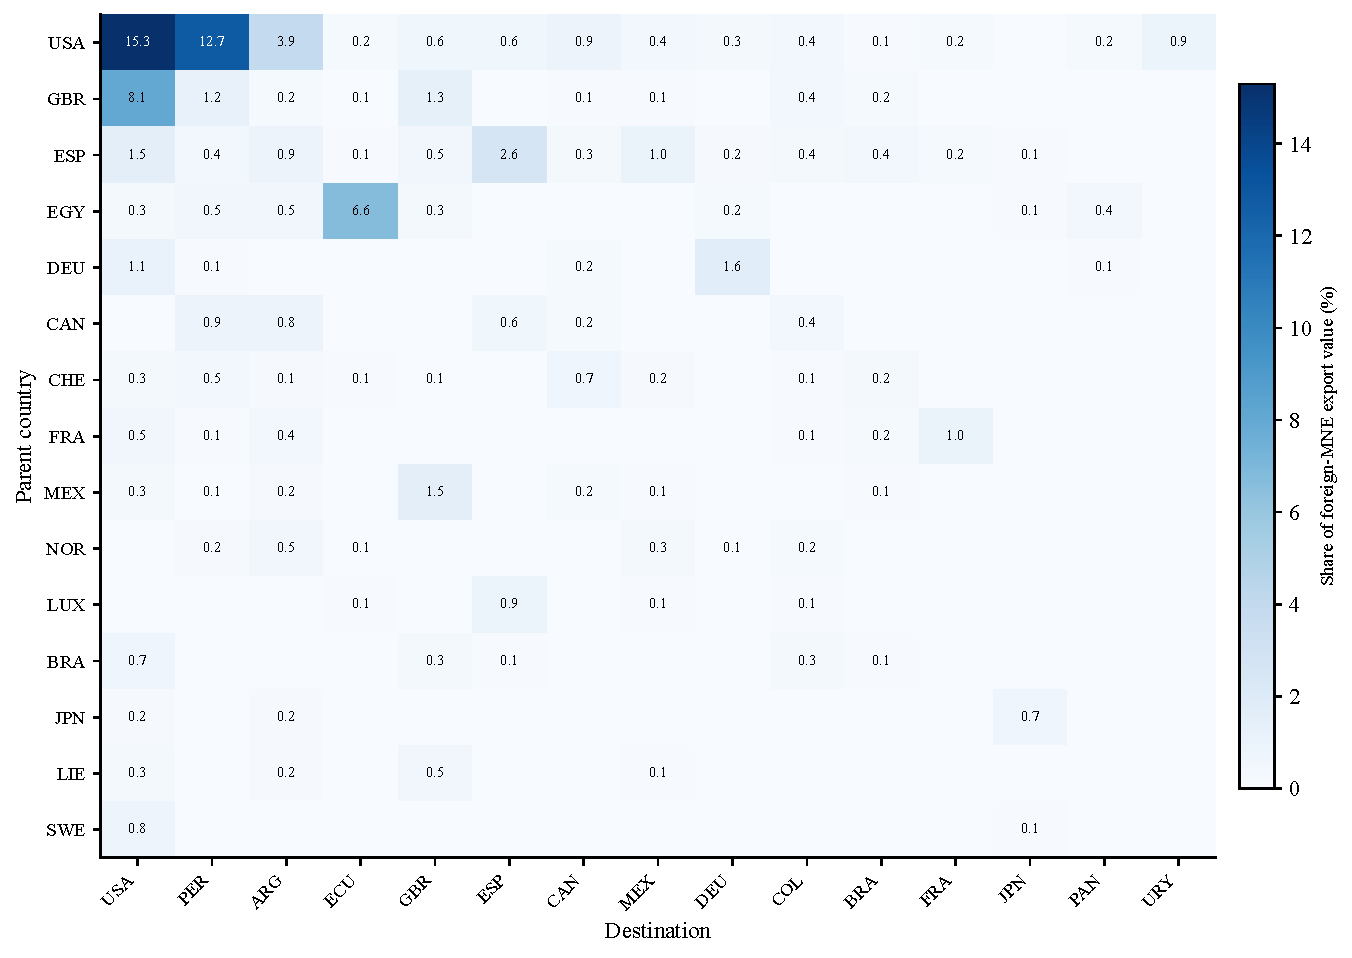
\includegraphics[width=1.0\textwidth,height=0.8\textheight,keepaspectratio]{figures/rest/fig_wp1d_heatmap_country_cellpct.pdf}%
  \caption{Other Goods: Foreign-Multinational Exports by Parent Country and Destination: Share of the Total}%
  \label{fig:hm_cell_rest}%
  \par\vspace{2pt}%
  \parbox{0.92\textwidth}{\footnotesize %
  \textit{Notes:} Percent of all foreign-MNE export value in each parent country and destination pair; fifteen largest parent countries and destinations.\\[3pt]%
  \textit{Source:} Authors' calculations based on customs data matched to Orbis and Dun \& Bradstreet.}%
  \end{figure}

\subsection{Exports to the Parent Country}
% ---- Figure: Other Goods: Share of Foreign-Multinational Exports Shipped to the Parent Country
\begin{figure}[H]\centering%
  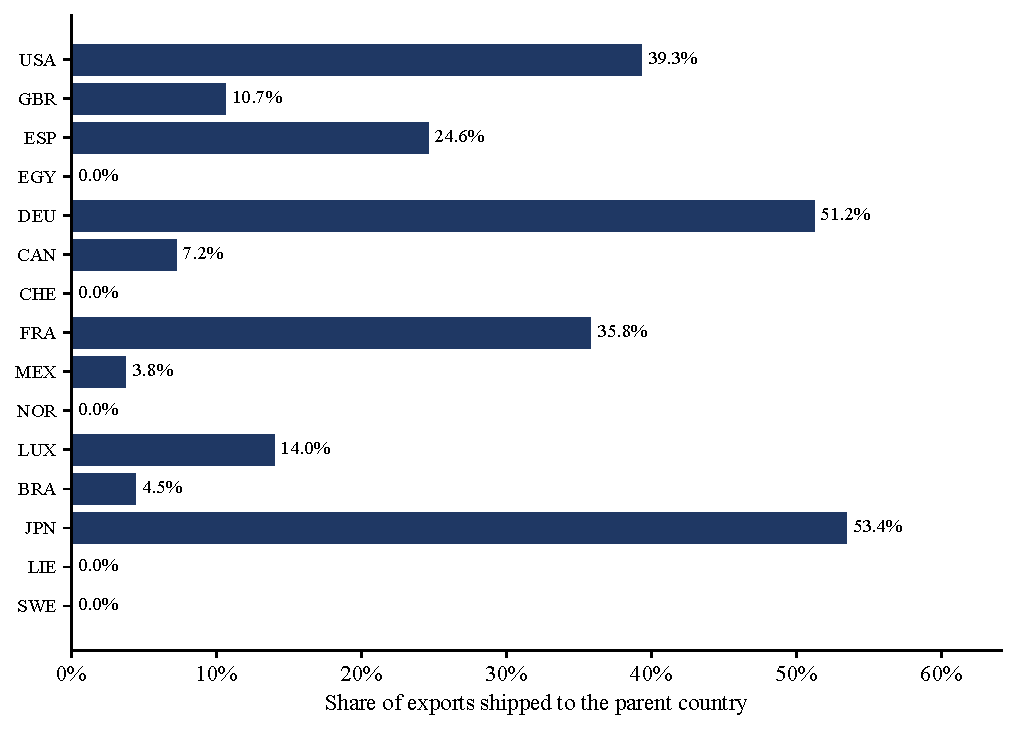
\includegraphics[width=0.85\textwidth,height=0.8\textheight,keepaspectratio]{figures/rest/fig_wp1d_home_share_by_parent.pdf}%
  \caption{Other Goods: Share of Foreign-Multinational Exports Shipped to the Parent Country}%
  \label{fig:home_rest}%
  \par\vspace{2pt}%
  \parbox{0.92\textwidth}{\footnotesize %
  \textit{Notes:} Percent of each parent country's exports shipped to that same country.\\[3pt]%
  \textit{Source:} Authors' calculations based on customs data matched to Orbis and Dun \& Bradstreet.}%
  \end{figure}
% ---- Table: Other Goods: Foreign-Multinational Exports to the Parent Countries, by Parent Country
\begin{table}[H]\centering\small%
  \caption{Other Goods: Foreign-Multinational Exports to the Parent Countries, by Parent Country}%
  \label{tab:pxp_rest}%
  \adjustbox{max width=\textwidth, max totalheight=0.8\textheight}{\begin{tabular}{lrrrrrrrrrrrr}
\toprule
Parent / Destination & USA & GBR & ESP & EGY & DEU & CAN & CHE & FRA & MEX & NOR & Other destinations & Total \\
\midrule
USA & 39.3 & 1.5 & 1.5 & 0.0 & 0.6 & 2.3 & 0.0 & 0.5 & 1.0 & 0.1 & 53.1 & 100.0 \\
GBR & 66.4 & 10.7 & 0.0 & 0.0 & 0.2 & 1.0 & 0.0 & 0.0 & 1.0 & 0.0 & 20.8 & 100.0 \\
ESP & 14.1 & 5.0 & 24.6 & 0.0 & 1.4 & 3.1 & 0.6 & 2.1 & 9.4 & 0.1 & 39.7 & 100.0 \\
EGY & 2.6 & 2.5 & 0.3 & 0.0 & 2.1 & 0.0 & 0.1 & 0.4 & 0.2 & 3.5 & 88.3 & 100.0 \\
DEU & 33.2 & 0.0 & 0.0 & 0.0 & 51.2 & 5.9 & 0.0 & 0.2 & 0.5 & 0.0 & 9.1 & 100.0 \\
CAN & 0.8 & 0.0 & 18.2 & 0.0 & 1.2 & 7.2 & 0.0 & 0.1 & 0.2 & 0.0 & 72.2 & 100.0 \\
CHE & 9.8 & 2.0 & 0.3 & 0.0 & 0.3 & 24.6 & 0.0 & 0.3 & 6.0 & 0.0 & 56.7 & 100.0 \\
FRA & 17.9 & 0.0 & 0.6 & 0.0 & 0.3 & 1.4 & 0.0 & 35.8 & 1.5 & 0.0 & 42.5 & 100.0 \\
MEX & 13.1 & 60.4 & 0.7 & 0.0 & 0.4 & 7.8 & 0.2 & 0.0 & 3.8 & 0.0 & 13.6 & 100.0 \\
NOR & 1.3 & 0.0 & 0.4 & 0.0 & 3.3 & 0.0 & 0.0 & 0.0 & 19.3 & 0.0 & 75.7 & 100.0 \\
Other parents & 21.8 & 8.1 & 9.4 & 0.0 & 1.7 & 2.7 & 2.1 & 0.5 & 3.9 & 0.0 & 49.8 & 100.0 \\
\bottomrule
\end{tabular}
}%
  \par\vspace{3pt}%
  \begin{minipage}{0.95\textwidth}\footnotesize %
  \textit{Notes:} Percent of each parent country's exports, by destination (rows add to 100). Destinations are the ten largest parent countries; the diagonal is the share shipped to the parent's own country.\\[3pt]%
  \textit{Source:} Authors' calculations based on customs data matched to Orbis and Dun \& Bradstreet.%
  \end{minipage}%
  \end{table}
% ---- Figure: Other Goods: Share of Foreign-Multinational Exports Shipped to the Parent Jurisdiction, Consolidated Parents
\begin{figure}[H]\centering%
  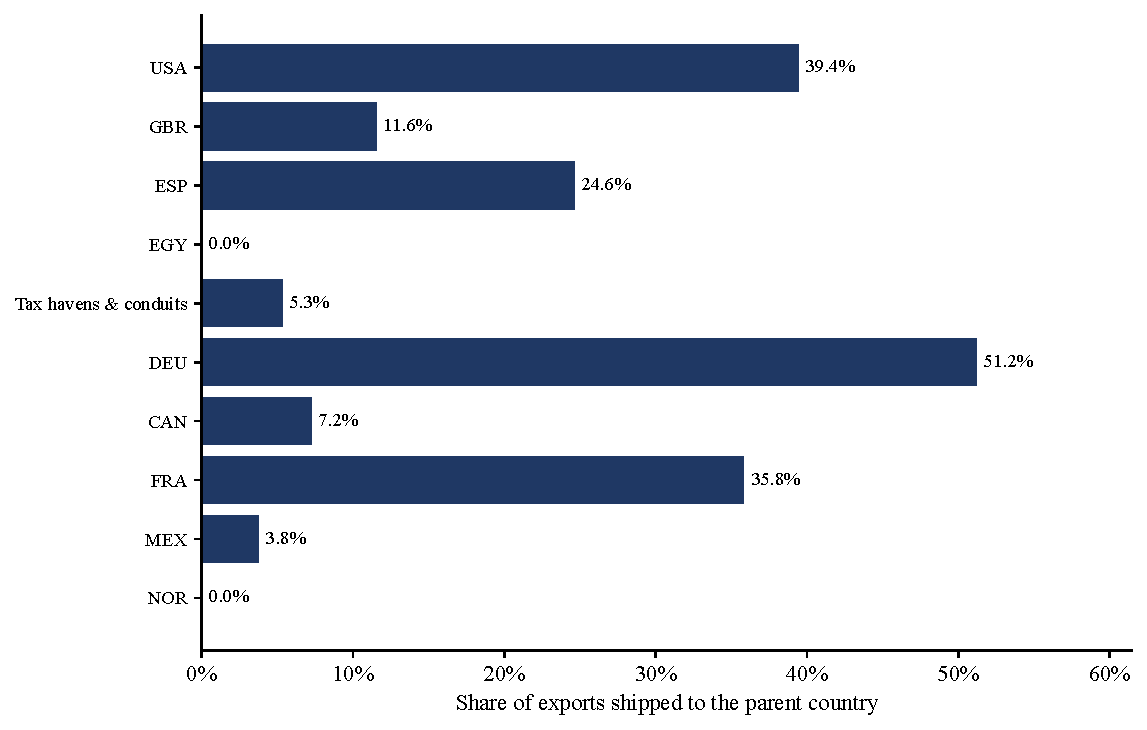
\includegraphics[width=0.85\textwidth,height=0.8\textheight,keepaspectratio]{figures/rest/fig_wp1d_home_share_by_parent_consolidated.pdf}%
  \caption{Other Goods: Share of Foreign-Multinational Exports Shipped to the Parent Jurisdiction, Consolidated Parents}%
  \label{fig:homec_rest}%
  \par\vspace{2pt}%
  \parbox{0.92\textwidth}{\footnotesize %
  \textit{Notes:} Percent of each parent's exports shipped to its own jurisdiction. Dependencies are assigned to their sovereign state and tax havens and conduit jurisdictions are pooled.\\[3pt]%
  \textit{Source:} Authors' calculations based on customs data matched to Orbis and Dun \& Bradstreet.}%
  \end{figure}
% ---- Table: Other Goods: Share of Foreign-Multinational Exports Shipped to the Parent Jurisdiction, Consolidated Parents
\begin{table}[H]\centering\small%
  \caption{Other Goods: Share of Foreign-Multinational Exports Shipped to the Parent Jurisdiction, Consolidated Parents}%
  \label{tab:homec_t_rest}%
  \adjustbox{max width=\textwidth, max totalheight=0.8\textheight}{\begin{tabular}{lrr}
\toprule
Consolidated parent & Home share (\%) & Exports (US\$bn/yr) \\
\midrule
USA & 39.4 & 0.1 \\
GBR & 11.6 & 0.0 \\
ESP & 24.6 & 0.0 \\
EGY & 0.0 & 0.0 \\
Tax havens \& conduits & 5.3 & 0.0 \\
DEU & 51.2 & 0.0 \\
CAN & 7.2 & 0.0 \\
FRA & 35.8 & 0.0 \\
MEX & 3.8 & 0.0 \\
NOR & 0.0 & 0.0 \\
\bottomrule
\end{tabular}
}%
  \par\vspace{3pt}%
  \begin{minipage}{0.95\textwidth}\footnotesize %
  \textit{Notes:} Home share: percent of the parent's exports shipped to its own jurisdiction. Values are annual averages in US\$ billion.\\[3pt]%
  \textit{Source:} Authors' calculations based on customs data matched to Orbis and Dun \& Bradstreet.%
  \end{minipage}%
  \end{table}
% ---- Figure: Other Goods: Share of Foreign-Multinational Exports Shipped to the Parent Jurisdiction
\begin{figure}[H]\centering%
  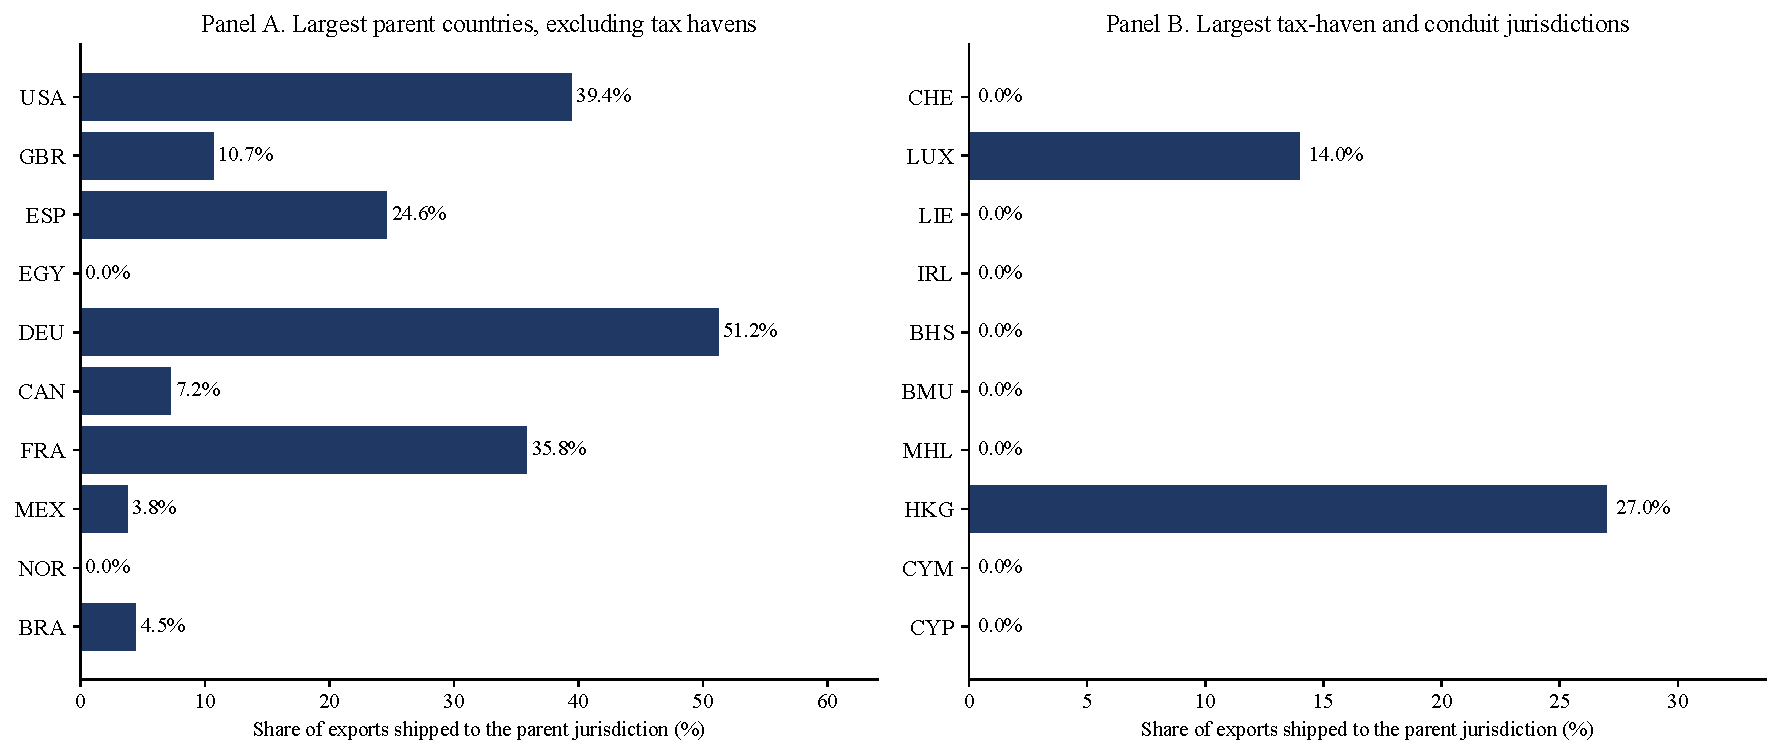
\includegraphics[width=1.0\textwidth,height=0.8\textheight,keepaspectratio]{figures/rest/fig_wp1d_home_share_haven_panels.pdf}%
  \caption{Other Goods: Share of Foreign-Multinational Exports Shipped to the Parent Jurisdiction}%
  \label{fig:homeh_rest}%
  \par\vspace{2pt}%
  \parbox{0.92\textwidth}{\footnotesize %
  \textit{Notes:} Percent of each parent jurisdiction's exports shipped to that same jurisdiction. Panel A: largest parent countries, excluding tax havens; dependencies are assigned to their sovereign state. Panel B: largest tax-haven and conduit jurisdictions.\\[3pt]%
  \textit{Source:} Authors' calculations based on customs data matched to Orbis and Dun \& Bradstreet.}%
  \end{figure}
% ---- Table: Other Goods: Share of Foreign-Multinational Exports Shipped to the Parent Jurisdiction
\begin{table}[H]\centering\small%
  \caption{Other Goods: Share of Foreign-Multinational Exports Shipped to the Parent Jurisdiction}%
  \label{tab:homeh_t_rest}%
  \adjustbox{max width=\textwidth, max totalheight=0.8\textheight}{\begin{tabular}{llrr}
\toprule
Panel & Parent & Home share (\%) & Exports (US\$bn/yr) \\
\midrule
Panel A & USA & 39.4 & 0.1 \\
Panel A & GBR & 10.7 & 0.0 \\
Panel A & ESP & 24.6 & 0.0 \\
Panel A & EGY & 0.0 & 0.0 \\
Panel A & DEU & 51.2 & 0.0 \\
Panel A & CAN & 7.2 & 0.0 \\
Panel A & FRA & 35.8 & 0.0 \\
Panel A & MEX & 3.8 & 0.0 \\
Panel A & NOR & 0.0 & 0.0 \\
Panel A & BRA & 4.5 & 0.0 \\
\midrule
Panel B & CHE & 0.0 & 0.0 \\
Panel B & LUX & 14.0 & 0.0 \\
Panel B & LIE & 0.0 & 0.0 \\
Panel B & IRL & 0.0 & 0.0 \\
Panel B & BHS & 0.0 & 0.0 \\
Panel B & BMU & 0.0 & 0.0 \\
Panel B & MHL & 0.0 & 0.0 \\
Panel B & HKG & 27.0 & 0.0 \\
Panel B & CYM & 0.0 & 0.0 \\
Panel B & CYP & 0.0 & 0.0 \\
\bottomrule
\end{tabular}
}%
  \par\vspace{3pt}%
  \begin{minipage}{0.95\textwidth}\footnotesize %
  \textit{Notes:} Home share: percent of the parent's exports shipped to its own jurisdiction. Panel A: largest parent countries, excluding tax havens. Panel B: largest tax-haven and conduit jurisdictions. Values are annual averages in US\$ billion.\\[3pt]%
  \textit{Source:} Authors' calculations based on customs data matched to Orbis and Dun \& Bradstreet.%
  \end{minipage}%
  \end{table}

\subsection{Destination Markets}
% ---- Figure: Other Goods: Exports to the United States, by Type of Exporter and Exporting Country
\begin{figure}[H]\centering%
  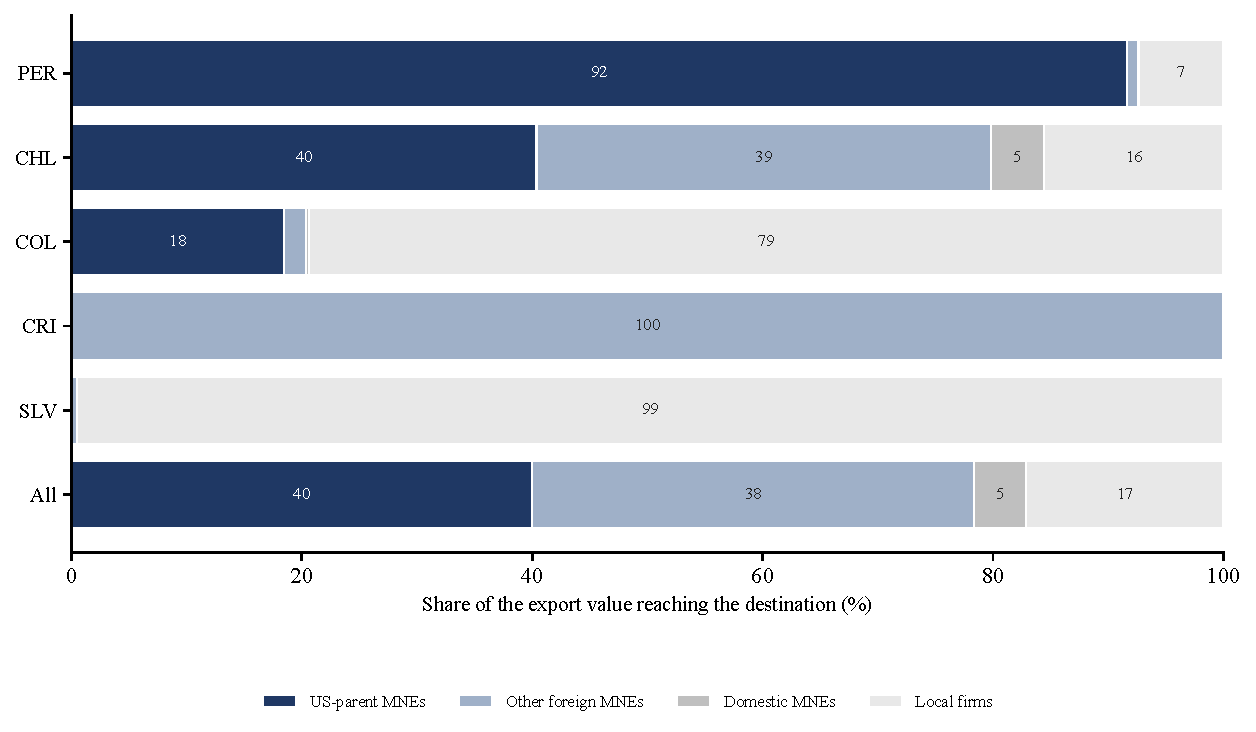
\includegraphics[width=0.9\textwidth,height=0.8\textheight,keepaspectratio]{figures/rest/fig_wp3_to_usa_carriers.pdf}%
  \caption{Other Goods: Exports to the United States, by Type of Exporter and Exporting Country}%
  \label{fig:to_usa_f_rest}%
  \par\vspace{2pt}%
  \parbox{0.92\textwidth}{\footnotesize %
  \textit{Notes:} Percent of each country's exports to the United States, by type of exporter.\\[3pt]%
  \textit{Source:} Authors' calculations based on customs data matched to Orbis and Dun \& Bradstreet.}%
  \end{figure}
% ---- Table: Other Goods: Exports to the United States, by Type of Exporter and Exporting Country
\begin{table}[H]\centering\small%
  \caption{Other Goods: Exports to the United States, by Type of Exporter and Exporting Country}%
  \label{tab:to_usa_rest}%
  \adjustbox{max width=\textwidth, max totalheight=0.8\textheight}{\begin{tabular}{lrrrrr}
\toprule
Origin & Exports to the USA (US\$bn/yr) & US-parent MNEs (\%) & Other foreign MNEs (\%) & Domestic MNEs (\%) & Local firms (\%) \\
\midrule
PER & 0.0 & 91.6 & 0.9 & 0.1 & 7.4 \\
CHL & 0.1 & 40.4 & 39.4 & 4.6 & 15.6 \\
COL & 0.0 & 18.4 & 1.9 & 0.2 & 79.4 \\
CRI & 0.0 & 0.0 & 100.0 & 0.0 & 0.0 \\
SLV & 0.0 & 0.0 & 0.5 & 0.0 & 99.5 \\
\midrule
All & 0.1 & 40.0 & 38.4 & 4.5 & 17.1 \\
\bottomrule
\end{tabular}
}%
  \par\vspace{3pt}%
  \begin{minipage}{0.95\textwidth}\footnotesize %
  \textit{Notes:} Percent of each country's exports to the United States, by type of exporter. Values are annual averages in US\$ billion.\\[3pt]%
  \textit{Source:} Authors' calculations based on customs data matched to Orbis and Dun \& Bradstreet.%
  \end{minipage}%
  \end{table}
% ---- Figure: Other Goods: Ownership of Exports to the Main Destination Markets
\begin{figure}[H]\centering%
  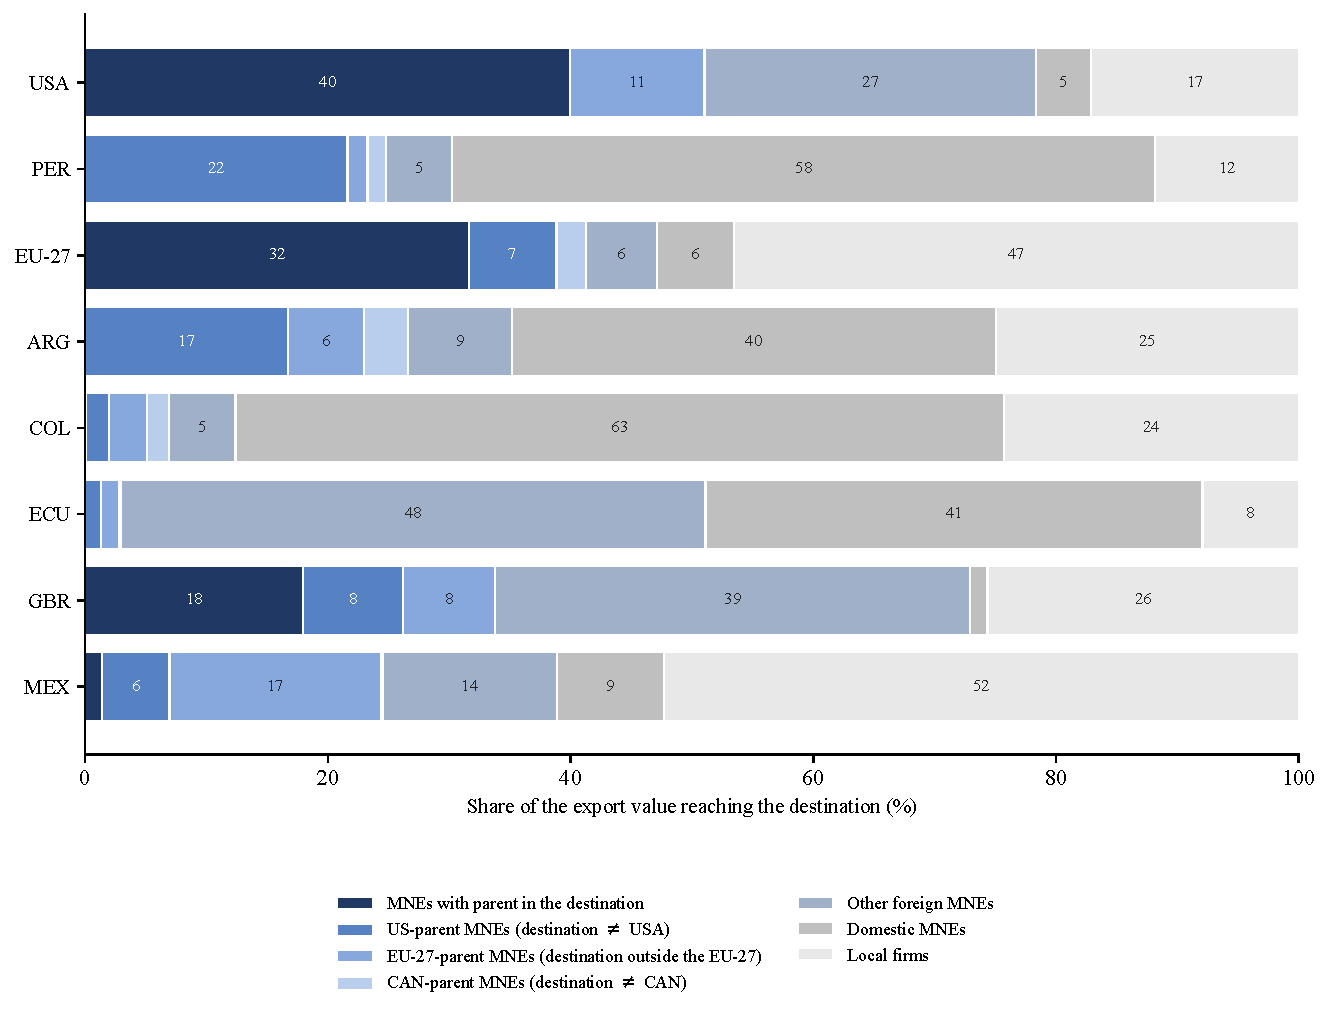
\includegraphics[width=0.95\textwidth,height=0.8\textheight,keepaspectratio]{figures/rest/fig_wp3_dest_carriers.pdf}%
  \caption{Other Goods: Ownership of Exports to the Main Destination Markets}%
  \label{fig:dest_f_rest}%
  \par\vspace{2pt}%
  \parbox{0.92\textwidth}{\footnotesize %
  \textit{Notes:} Percent of the export value reaching each destination, by type of exporter. The first segment is exports by MNEs whose parent is located in that destination. EU-27 member states are pooled.\\[3pt]%
  \textit{Source:} Authors' calculations based on customs data matched to Orbis and Dun \& Bradstreet.}%
  \end{figure}
% ---- Table: Other Goods: Ownership of Exports to the Main Destination Markets
\begin{table}[H]\centering\footnotesize%
  \caption{Other Goods: Ownership of Exports to the Main Destination Markets}%
  \label{tab:dest_rest}%
  \adjustbox{max width=\textwidth, max totalheight=0.8\textheight}{\begin{tabular}{lrrrrrrrr}
\toprule
Destination & \multicolumn{1}{p{1.5cm}}{\raggedright Exports (US\$bn/yr)} & \multicolumn{1}{p{2.2cm}}{\raggedright MNEs with parent in the destination (\%)} & \multicolumn{1}{p{1.6cm}}{\raggedright US-parent MNEs (\%)} & \multicolumn{1}{p{1.6cm}}{\raggedright EU-27-parent MNEs (\%)} & \multicolumn{1}{p{1.6cm}}{\raggedright CAN-parent MNEs (\%)} & \multicolumn{1}{p{1.6cm}}{\raggedright Other foreign MNEs (\%)} & \multicolumn{1}{p{1.6cm}}{\raggedright Domestic MNEs (\%)} & \multicolumn{1}{p{1.5cm}}{\raggedright Local firms (\%)} \\
\midrule
USA & 0.1 & 40.0 & -- & 11.0 & 0.1 & 27.3 & 4.5 & 17.1 \\
PER & 0.1 & 0.0 & 21.6 & 1.6 & 1.5 & 5.5 & 57.9 & 11.8 \\
EU-27 & 0.1 & 31.6 & 7.2 & -- & 2.4 & 5.8 & 6.3 & 46.6 \\
ARG & 0.0 & 0.0 & 16.7 & 6.2 & 3.6 & 8.5 & 39.9 & 25.0 \\
COL & 0.0 & 0.0 & 2.0 & 3.1 & 1.8 & 5.5 & 63.3 & 24.3 \\
ECU & 0.0 & 0.0 & 1.3 & 1.5 & 0.2 & 48.2 & 40.9 & 7.9 \\
GBR & 0.0 & 18.0 & 8.3 & 7.6 & 0.0 & 39.1 & 1.4 & 25.6 \\
MEX & 0.0 & 1.4 & 5.5 & 17.4 & 0.1 & 14.4 & 8.8 & 52.3 \\
\bottomrule
\end{tabular}
}%
  \par\vspace{3pt}%
  \begin{minipage}{0.95\textwidth}\footnotesize %
  \textit{Notes:} Percent of the export value reaching each destination, by type of exporter. EU-27 member states are pooled. Values are annual averages in US\$ billion.\\[3pt]%
  \textit{Source:} Authors' calculations based on customs data matched to Orbis and Dun \& Bradstreet.%
  \end{minipage}%
  \end{table}

\section{Fact 4: A Small Set of Large Multinational Groups Accounts for Most Exports}\label{sec:f4s_rest}

\subsection{Size of the Group's Global Network}
% ---- Figure: Other Goods: Foreign-Multinational Exports and Number of Parents, by Size of the Group's Global Network
\begin{figure}[H]\centering%
  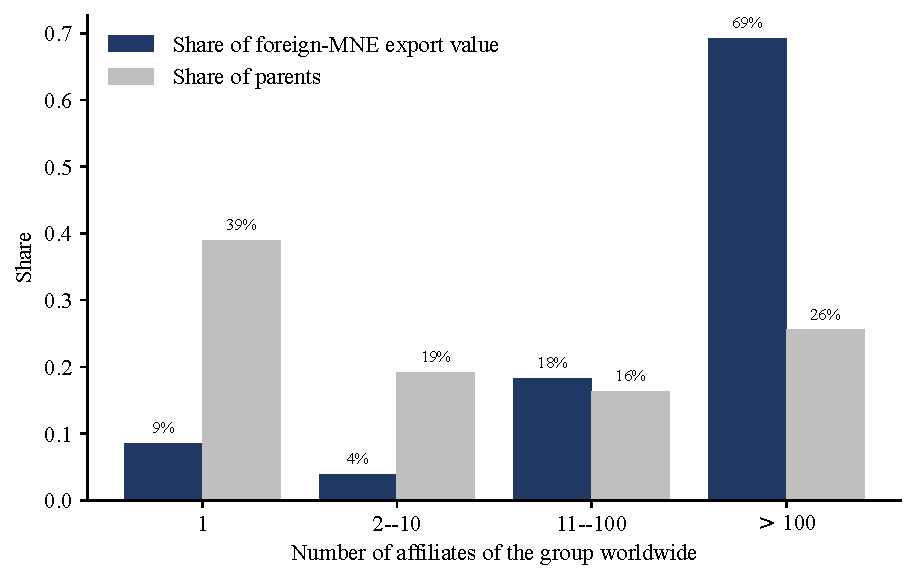
\includegraphics[width=0.7\textwidth,height=0.8\textheight,keepaspectratio]{figures/rest/fig_wp0_fig5_network.pdf}%
  \caption{Other Goods: Foreign-Multinational Exports and Number of Parents, by Size of the Group's Global Network}%
  \label{fig:net_rest}%
  \par\vspace{2pt}%
  \parbox{0.92\textwidth}{\footnotesize %
  \textit{Notes:} Shares of foreign-MNE export value and of parents, by the number of affiliates the group has worldwide.\\[3pt]%
  \textit{Source:} Authors' calculations based on customs data matched to Orbis and Dun \& Bradstreet.}%
  \end{figure}
% ---- Table: Other Goods: Foreign-Multinational Exports and Number of Parents, by Size of the Group's Global Network
\begin{table}[H]\centering\small%
  \caption{Other Goods: Foreign-Multinational Exports and Number of Parents, by Size of the Group's Global Network}%
  \label{tab:net_t_rest}%
  \adjustbox{max width=\textwidth, max totalheight=0.8\textheight}{\begin{tabular}{lrrr}
\toprule
Affiliates worldwide & Parents & Share of parents (\%) & Share of foreign-MNE export value (\%) \\
\midrule
1 & 221 & 38.9 & 8.5 \\
2--10 & 109 & 19.2 & 3.9 \\
11--100 & 93 & 16.4 & 18.3 \\
$>$100 & 145 & 25.5 & 69.2 \\
\midrule
All parents & 568 & 100 & 100 \\
\bottomrule
\end{tabular}
}%
  \par\vspace{3pt}%
  \begin{minipage}{0.95\textwidth}\footnotesize %
  \textit{Notes:} Number and share of parents, and share of foreign-MNE export value, by the number of affiliates the group has worldwide.\\[3pt]%
  \textit{Source:} Authors' calculations based on customs data matched to Orbis and Dun \& Bradstreet.%
  \end{minipage}%
  \end{table}

\subsection{Concentration within Products}
% ---- Figure: Other Goods: Export Concentration within Products: Firms and Groups
\begin{figure}[H]\centering%
  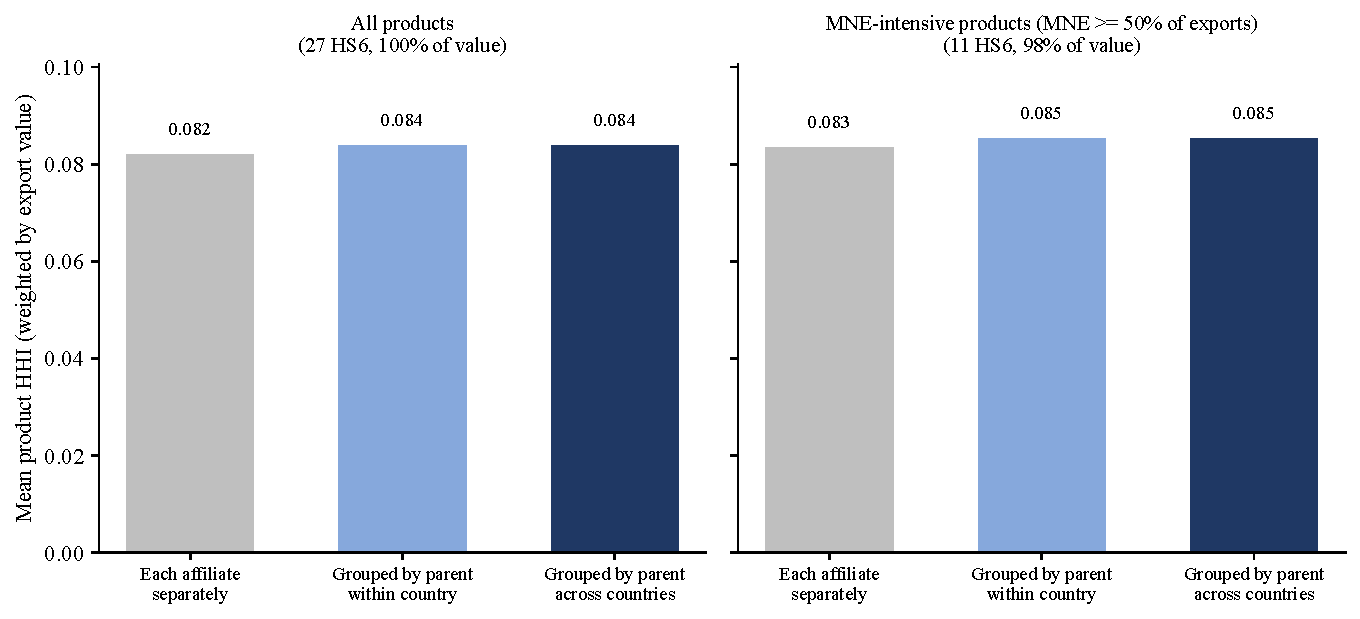
\includegraphics[width=0.9\textwidth,height=0.8\textheight,keepaspectratio]{figures/rest/fig_wp0_fig6_hhi.pdf}%
  \caption{Other Goods: Export Concentration within Products: Firms and Groups}%
  \label{fig:hhi_rest}%
  \par\vspace{2pt}%
  \parbox{0.92\textwidth}{\footnotesize %
  \textit{Notes:} Mean Herfindahl index of exporters within each HS6 product, weighted by export value, counting each affiliate separately or grouping affiliates by parent within or across countries. Right panel: products where MNEs account for at least half of exports.\\[3pt]%
  \textit{Source:} Authors' calculations based on customs data matched to Orbis and Dun \& Bradstreet.}%
  \end{figure}
% ---- Table: Other Goods: Export Concentration within Products: Firms and Groups
\begin{table}[H]\centering\small%
  \caption{Other Goods: Export Concentration within Products: Firms and Groups}%
  \label{tab:hhi_t_rest}%
  \adjustbox{max width=\textwidth, max totalheight=0.8\textheight}{\begin{tabular}{llrrr}
\toprule
Sample & Measure & Firm level & Groups within country & Groups across countries \\
\midrule
\multicolumn{5}{l}{\textit{All products: 27 HS6, 100\% of value}} \\
 & Mean HHI & 0.082 & 0.084 & 0.084 \\
 & Mean top-exporter share & 24.9\% & 24.9\% & 24.9\% \\
 & Effective number of exporters (1/HHI) & 18.3 & 17.7 & 17.7 \\
\multicolumn{5}{l}{\textit{MNE-intensive products (MNE $\geq$ 50\% of exports): 11 HS6, 98\% of value}} \\
 & Mean HHI & 0.083 & 0.085 & 0.085 \\
 & Mean top-exporter share & 25.2\% & 25.2\% & 25.2\% \\
 & Effective number of exporters (1/HHI) & 13.2 & 12.6 & 12.6 \\
\bottomrule
\end{tabular}
}%
  \par\vspace{3pt}%
  \begin{minipage}{0.95\textwidth}\footnotesize %
  \textit{Notes:} Means across HS6 products, weighted by export value. Firm level: each affiliate counted separately. Groups: affiliates grouped by ultimate parent within each exporting country or across countries.\\[3pt]%
  \textit{Source:} Authors' calculations based on customs data matched to Orbis and Dun \& Bradstreet.%
  \end{minipage}%
  \end{table}

\subsection{Groups and Affiliates}
% ---- Table: Other Goods: Multinational Affiliates and Groups in Origin--Destination--Product--Year Cells
\begin{table}[H]\centering\small%
  \caption{Other Goods: Multinational Affiliates and Groups in Origin--Destination--Product--Year Cells}%
  \label{tab:grp_rest}%
  \adjustbox{max width=\textwidth, max totalheight=0.8\textheight}{\begin{tabular}{lr}
\toprule
Origin-destination-product-year cells with $\geq 1$ MNE & \\
\midrule
Cells & 2,372 \\
MNE affiliates per cell (mean) & 5.05 \\
MNE groups per cell (mean) & 4.95 \\
Affiliates per group, pooled & 1.02 \\
Affiliates per group, mean weighted by export value & 1.03 \\
Cells where one group exports through $>1$ affiliate (\%) & 8.4 \\
\bottomrule
\end{tabular}
}%
  \par\vspace{3pt}%
  \begin{minipage}{0.95\textwidth}\footnotesize %
  \textit{Notes:} Cells with at least one MNE. Group: ultimate parent in Orbis or Dun \& Bradstreet (parent name when the identifier is missing).\\[3pt]%
  \textit{Source:} Authors' calculations based on customs data matched to Orbis and Dun \& Bradstreet.%
  \end{minipage}%
  \end{table}
% ---- Table: Other Goods: Multinational Presence and Exports: Affiliates and Groups
\begin{table}[H]\centering\small%
  \caption{Other Goods: Multinational Presence and Exports: Affiliates and Groups}%
  \label{tab:grp_r_rest}%
  \adjustbox{max width=\textwidth, max totalheight=0.8\textheight}{\begin{tabular}{lcccccc} \hline
 & \multicolumn{3}{c}{Origin $\times$ year, destination $\times$ year, product FE} & \multicolumn{3}{c}{Origin $\times$ dest. $\times$ product, origin $\times$ dest. $\times$ year FE} \\
 & (1) & (2) & (3) & (4) & (5) & (6) \\ \hline
\multicolumn{7}{l}{\textit{Panel A. Dependent variable: $\ln$ exports, all firms}} \\
$\ln$(\# MNE firms) & 1.8402*** &  &  & 1.1124*** &  &  \\
 & (0.1590) &  &  & (0.2255) &  &  \\
$\ln$(\# MNE groups) &  & 1.8312*** & 1.8391*** &  & 1.1119*** & 1.1077*** \\
 &  & (0.1604) & (0.1588) &  & (0.2265) & (0.2270) \\
$\ln$(affiliates per group) &  &  & 2.3965** &  &  & 1.3037 \\
 &  &  & (0.9466) &  &  & (1.7782) \\
\midrule
\multicolumn{7}{l}{\textit{Panel B. Dependent variable: $\ln$ exports, non-MNE firms}} \\
$\ln$(\# MNE firms) & 1.2338*** &  &  & 0.6712* &  &  \\
 & (0.2149) &  &  & (0.3739) &  &  \\
$\ln$(\# MNE groups) &  & 1.2217*** & 1.2370*** &  & 0.6829* & 0.6460* \\
 &  & (0.2128) & (0.2163) &  & (0.3667) & (0.3712) \\
$\ln$(affiliates per group) &  &  & 2.8459* &  &  & -4.9065 \\
 &  &  & (1.5421) &  &  & (4.0733) \\
\hline
Product FE & $\checkmark$ & $\checkmark$ & $\checkmark$ &  &  &  \\
Origin $\times$ year FE & $\checkmark$ & $\checkmark$ & $\checkmark$ &  &  &  \\
Destination $\times$ year FE & $\checkmark$ & $\checkmark$ & $\checkmark$ &  &  &  \\
Origin $\times$ dest.\ $\times$ product FE &  &  &  & $\checkmark$ & $\checkmark$ & $\checkmark$ \\
Origin $\times$ dest.\ $\times$ year FE &  &  &  & $\checkmark$ & $\checkmark$ & $\checkmark$ \\
Observations (Panel A) & 1,333 & 1,333 & 1,333 & 641 & 641 & 641 \\
Observations (Panel B) & 767 & 767 & 767 & 204 & 204 & 204 \\
\hline
\end{tabular}
}%
  \par\vspace{3pt}%
  \begin{minipage}{0.95\textwidth}\footnotesize %
  \textit{Notes:} Observations are origin--destination--HS6--year cells. Other Goods products only. Dependent variable: $\ln$ exports of the cell (Panel A) and of the non-MNE firms in the cell (Panel B). Regressors: $\ln$ number of MNE affiliates or $\ln$ number of MNE groups (distinct ultimate parents). Standard errors clustered by origin--destination pair in parentheses. *** $p<0.01$, ** $p<0.05$, * $p<0.1$.\\[3pt]%
  \textit{Source:} Authors' calculations based on customs data matched to Orbis and Dun \& Bradstreet.%
  \end{minipage}%
  \end{table}

\section{Fact 5: Multinational Presence Is Associated with Higher Exports}\label{sec:f5_rest}
% ---- Table: Other Goods: Multinational Presence and Exports
\begin{table}[H]\centering\small%
  \caption{Other Goods: Multinational Presence and Exports}%
  \label{tab:t1_rest}%
  \adjustbox{max width=\textwidth, max totalheight=0.8\textheight}{\begin{tabular}{lcccccc} \hline
 & \multicolumn{3}{c}{Intensive: $\ln$(\# MNE firms)} & \multicolumn{3}{c}{Extensive: any MNE present} \\
 & (1) & (2) & (3) & (1) & (2) & (3) \\ \hline
\multicolumn{7}{l}{\textit{Panel A. Dependent variable: $\ln$ exports, all firms}} \\
$\ln$(\# MNE firms) & 1.8059*** & 1.8402*** & 1.1124*** &  &  &  \\
 & (0.1087) & (0.1590) & (0.2255) &  &  &  \\
Any MNE present &  &  &  & 0.1214 & 0.2291 & 1.0052*** \\
 &  &  &  & (0.1490) & (0.2076) & (0.3256) \\
\midrule
\multicolumn{7}{l}{\textit{Panel B. Dependent variable: $\ln$ exports, non-MNE firms}} \\
$\ln$(\# MNE firms) & 0.9826*** & 1.2338*** & 0.6712* &  &  &  \\
 & (0.1424) & (0.2149) & (0.3739) &  &  &  \\
Any MNE present &  &  &  & 0.4614*** & 0.5217** & 0.6655 \\
 &  &  &  & (0.1490) & (0.2381) & (0.5481) \\
\hline
Origin FE & $\checkmark$ &  &  & $\checkmark$ &  &  \\
Destination FE & $\checkmark$ &  &  & $\checkmark$ &  &  \\
Product FE & $\checkmark$ & $\checkmark$ &  & $\checkmark$ & $\checkmark$ &  \\
Year FE & $\checkmark$ &  &  & $\checkmark$ &  &  \\
Origin $\times$ year FE &  & $\checkmark$ &  &  & $\checkmark$ &  \\
Destination $\times$ year FE &  & $\checkmark$ &  &  & $\checkmark$ &  \\
Origin $\times$ dest.\ $\times$ product FE &  &  & $\checkmark$ &  &  & $\checkmark$ \\
Origin $\times$ dest.\ $\times$ year FE &  &  & $\checkmark$ &  &  & $\checkmark$ \\
Observations (Panel A) & 2,350 & 1,333 & 641 & 3,831 & 2,928 & 903 \\
Observations (Panel B) & 1,330 & 767 & 204 & 2,793 & 2,125 & 383 \\
\hline
\end{tabular}
}%
  \par\vspace{3pt}%
  \begin{minipage}{0.95\textwidth}\footnotesize %
  \textit{Notes:} Observations are origin--destination--HS6--year cells. Other Goods products only. Dependent variable: $\ln$ exports of the cell (Panel A) and of the non-MNE firms in the cell (Panel B). Intensive margin: $\ln$ number of MNEs, cells with at least one MNE. Extensive margin: indicator for at least one MNE. Standard errors clustered by origin--destination pair in parentheses. *** $p<0.01$, ** $p<0.05$, * $p<0.1$.\\[3pt]%
  \textit{Source:} Authors' calculations based on customs data matched to Orbis and Dun \& Bradstreet.%
  \end{minipage}%
  \end{table}
% ---- Table: Other Goods: Multinational Exports by Exporting Country and Destination Type
\begin{table}[H]\centering\small%
  \caption{Other Goods: Multinational Exports by Exporting Country and Destination Type}%
  \label{tab:pres_rest}%
  \adjustbox{max width=\textwidth, max totalheight=0.8\textheight}{\begin{tabular}{lrrrrr}
\toprule
Origin & MNE value (US\$bn/yr) & of which domestic (\%) & Foreign-MNE value (US\$bn/yr) & \multicolumn{2}{c}{\% of foreign-MNE value, by destination} \\
 & & & & parent country & other (of which: group affiliate there) \\
\midrule
CHL & 0.4 & 37.0 & 0.2 & 18.7 & 81.3 (37.2) \\
COL & 0.0 & 4.4 & 0.0 & 34.5 & 65.5 (9.8) \\
CRI & 0.0 & 0.0 & 0.0 & 0.0 & 100.0 (0.0) \\
PER & 0.0 & 1.0 & 0.0 & 84.9 & 15.1 (0.2) \\
SLV & 0.0 & 0.0 & 0.0 & 4.6 & 95.4 (3.3) \\
\midrule
All & 0.4 & 36.9 & 0.2 & 18.8 & 81.2 (37.0) \\
\bottomrule
\end{tabular}
}%
  \par\vspace{3pt}%
  \begin{minipage}{0.95\textwidth}\footnotesize %
  \textit{Notes:} MNE and foreign-MNE export value by country, and the split of foreign-MNE value by destination. Parent country: exports to the country of the ultimate parent. Other: all remaining destinations; in parentheses, destinations where the group has another affiliate. Values are annual averages in US\$ billion.\\[3pt]%
  \textit{Source:} Authors' calculations based on customs data matched to Orbis and Dun \& Bradstreet.%
  \end{minipage}%
  \end{table}
% ---- Table: Other Goods: Multinational Presence and Exports: Intensive Margin, by Type of Multinational
\begin{table}[H]\centering\small%
  \caption{Other Goods: Multinational Presence and Exports: Intensive Margin, by Type of Multinational}%
  \label{tab:cnt_rest}%
  \adjustbox{max width=\textwidth, max totalheight=0.8\textheight}{\begin{tabular}{lcccccc} \hline
 & \multicolumn{2}{c}{All MNEs} & \multicolumn{2}{c}{Foreign / domestic} & \multicolumn{2}{c}{Foreign by destination, domestic} \\
 & (1) & (2) & (3) & (4) & (5) & (6) \\ \hline
\multicolumn{7}{l}{\textit{Panel A. Dependent variable: $\ln$ exports, all firms}} \\
$\ln$(\# MNE firms) & 1.8402*** & 1.1124*** &  &  &  &  \\
 & (0.1590) & (0.2255) &  &  &  &  \\
$\ln$(\# foreign MNEs) &  &  & 1.2219*** & 0.7610* &  &  \\
 &  &  & (0.2567) & (0.3809) &  &  \\
$\ln$(\# domestic MNEs) &  &  & 0.6260 & -0.0815 &  &  \\
 &  &  & (0.3832) & (0.1748) &  &  \\
\midrule
\multicolumn{7}{l}{\textit{Panel B. Dependent variable: $\ln$ exports, non-MNE firms}} \\
$\ln$(\# MNE firms) & 1.2338*** & 0.6712* &  &  &  &  \\
 & (0.2149) & (0.3739) &  &  &  &  \\
$\ln$(\# foreign MNEs) &  &  & 0.2490 & 0.2668* &  &  \\
 &  &  & (0.3400) & (0.1164) &  &  \\
$\ln$(\# domestic MNEs) &  &  & 0.7441 & 0.0365 &  &  \\
 &  &  & (0.5034) & (0.5349) &  &  \\
\hline
Product FE & $\checkmark$ &  & $\checkmark$ &  & $\checkmark$ &  \\
Origin $\times$ year FE & $\checkmark$ &  & $\checkmark$ &  & $\checkmark$ &  \\
Destination $\times$ year FE & $\checkmark$ &  & $\checkmark$ &  & $\checkmark$ &  \\
Origin $\times$ dest.\ $\times$ product FE &  & $\checkmark$ &  & $\checkmark$ &  & $\checkmark$ \\
Origin $\times$ dest.\ $\times$ year FE &  & $\checkmark$ &  & $\checkmark$ &  & $\checkmark$ \\
Observations (Panel A) & 1,333 & 641 & 145 & 70 & 141 & 141 \\
Observations (Panel B) & 767 & 204 & 125 & 54 & 139 & 139 \\
\hline
\end{tabular}
}%
  \par\vspace{3pt}%
  \begin{minipage}{0.95\textwidth}\footnotesize %
  \textit{Notes:} Observations are origin--destination--HS6--year cells. Other Goods products only. Dependent variable: $\ln$ exports of the cell (Panel A) and of the non-MNE firms in the cell (Panel B). Regressors: $\ln$ number of MNEs of each type. Columns (5)--(6) split foreign MNEs by whether the destination is the parent's country. Standard errors clustered by origin--destination pair in parentheses. *** $p<0.01$, ** $p<0.05$, * $p<0.1$.\\[3pt]%
  \textit{Source:} Authors' calculations based on customs data matched to Orbis and Dun \& Bradstreet.%
  \end{minipage}%
  \end{table}
% ---- Table: Other Goods: Multinational Presence and Exports: Extensive Margin, by Type of Multinational
\begin{table}[H]\centering\small%
  \caption{Other Goods: Multinational Presence and Exports: Extensive Margin, by Type of Multinational}%
  \label{tab:ext_rest}%
  \adjustbox{max width=\textwidth, max totalheight=0.8\textheight}{\begin{tabular}{lcccccc} \hline
 & \multicolumn{2}{c}{All MNEs} & \multicolumn{2}{c}{Foreign / domestic} & \multicolumn{2}{c}{Foreign by destination, domestic} \\
 & (1) & (2) & (3) & (4) & (5) & (6) \\ \hline
\multicolumn{7}{l}{\textit{Panel A. Dependent variable: $\ln$ exports, all firms}} \\
Any MNE present & 0.2291 & 1.0052*** &  &  &  &  \\
 & (0.2076) & (0.3256) &  &  &  &  \\
Any foreign MNE &  &  & 0.5417*** & 0.7689** &  &  \\
 &  &  & (0.1593) & (0.3199) &  &  \\
Any foreign MNE, parent-country destination &  &  &  &  & 1.6482*** & 0.8616** \\
 &  &  &  &  & (0.2403) & (0.3835) \\
Any foreign MNE, other destination &  &  &  &  & 0.4937*** & 0.4724 \\
 &  &  &  &  & (0.1689) & (0.3114) \\
Any domestic MNE &  &  & 2.6655*** & 0.8535*** & 2.4719*** & 0.8036** \\
 &  &  & (0.2144) & (0.2919) & (0.2184) & (0.3075) \\
\midrule
\multicolumn{7}{l}{\textit{Panel B. Dependent variable: $\ln$ exports, non-MNE firms}} \\
Any MNE present & 0.5217** & 0.6655 &  &  &  &  \\
 & (0.2381) & (0.5481) &  &  &  &  \\
Any foreign MNE &  &  & 0.4939** & 0.3217 &  &  \\
 &  &  & (0.2196) & (0.5881) &  &  \\
Any foreign MNE, parent-country destination &  &  &  &  & 1.0152*** & 0.4587 \\
 &  &  &  &  & (0.2936) & (0.2979) \\
Any foreign MNE, other destination &  &  &  &  & 0.5331** & 0.2250 \\
 &  &  &  &  & (0.2189) & (0.5351) \\
Any domestic MNE &  &  & 1.4052*** & 0.3147 & 1.2667*** & 0.2834 \\
 &  &  & (0.2128) & (0.5086) & (0.2017) & (0.5337) \\
\hline
Product FE & $\checkmark$ &  & $\checkmark$ &  & $\checkmark$ &  \\
Origin $\times$ year FE & $\checkmark$ &  & $\checkmark$ &  & $\checkmark$ &  \\
Destination $\times$ year FE & $\checkmark$ &  & $\checkmark$ &  & $\checkmark$ &  \\
Origin $\times$ dest.\ $\times$ product FE &  & $\checkmark$ &  & $\checkmark$ &  & $\checkmark$ \\
Origin $\times$ dest.\ $\times$ year FE &  & $\checkmark$ &  & $\checkmark$ &  & $\checkmark$ \\
Observations (Panel A) & 2,928 & 903 & 2,928 & 903 & 2,928 & 903 \\
Observations (Panel B) & 2,125 & 383 & 2,125 & 383 & 2,125 & 383 \\
\hline
\end{tabular}
}%
  \par\vspace{3pt}%
  \begin{minipage}{0.95\textwidth}\footnotesize %
  \textit{Notes:} Observations are origin--destination--HS6--year cells. Other Goods products only. Dependent variable: $\ln$ exports of the cell (Panel A) and of the non-MNE firms in the cell (Panel B). Regressors: indicators for at least one MNE of each type. Columns (5)--(6) split foreign MNEs by whether the destination is the parent's country. Standard errors clustered by origin--destination pair in parentheses. *** $p<0.01$, ** $p<0.05$, * $p<0.1$.\\[3pt]%
  \textit{Source:} Authors' calculations based on customs data matched to Orbis and Dun \& Bradstreet.%
  \end{minipage}%
  \end{table}

\section{Fact 6: Distance Is a Weaker Barrier for Multinationals}\label{sec:f6_rest}
% ---- Table: Other Goods: Distance and Firm Exports: Multinationals by Presence at the Destination
\begin{table}[H]\centering\small%
  \caption{Other Goods: Distance and Firm Exports: Multinationals by Presence at the Destination}%
  \label{tab:t2_rest}%
  \adjustbox{max width=\textwidth, max totalheight=0.8\textheight}{\begin{tabular}{lcccc} \hline
Dep.\ var.: $\ln$ exports & (1) & (2) & (3) & (4) \\ \hline
$\ln$ distance & -0.0720 & -0.0574 & -0.0698 & -0.0545 \\
 & (0.1077) & (0.1025) & (0.1080) & (0.1023) \\
$\ln$ distance $\times$ MNE & -0.0086 & 0.0029 &  &  \\
 & (0.0109) & (0.0103) &  &  \\
$\ln$ distance $\times$ MNE, present at destination &  &  & 0.0308 & 0.0405** \\
 &  &  & (0.0189) & (0.0185) \\
$\ln$ distance $\times$ MNE, not present at destination &  &  & -0.0270*** & -0.0151* \\
 &  &  & (0.0088) & (0.0084) \\
\hline
Origin FE & $\checkmark$ &  & $\checkmark$ &  \\
Destination FE & $\checkmark$ &  & $\checkmark$ &  \\
Year FE & $\checkmark$ &  & $\checkmark$ &  \\
Origin $\times$ year FE &  & $\checkmark$ &  & $\checkmark$ \\
Destination $\times$ year FE &  & $\checkmark$ &  & $\checkmark$ \\
Product FE & $\checkmark$ & $\checkmark$ & $\checkmark$ & $\checkmark$ \\
\hline
Observations & 38,597 & 38,110 & 38,597 & 38,110 \\
\hline
\end{tabular}
}%
  \par\vspace{3pt}%
  \begin{minipage}{0.95\textwidth}\footnotesize %
  \textit{Notes:} Observations are firm--destination--HS6--year cells. Other Goods products only. Dependent variable: $\ln$ exports. Non-MNE firms are the omitted group. Present: the group has an affiliate in the destination or the destination is the parent's country. Standard errors clustered by origin--destination pair in parentheses. *** $p<0.01$, ** $p<0.05$, * $p<0.1$.\\[3pt]%
  \textit{Source:} Authors' calculations based on customs data matched to Orbis and Dun \& Bradstreet.%
  \end{minipage}%
  \end{table}
% ---- Table: Other Goods: Distance and Firm Exports: Foreign and Domestic Multinationals
\begin{table}[H]\centering\small%
  \caption{Other Goods: Distance and Firm Exports: Foreign and Domestic Multinationals}%
  \label{tab:dist_rest}%
  \adjustbox{max width=\textwidth, max totalheight=0.8\textheight}{\begin{tabular}{lcccc} \hline
Dep.\ var.: $\ln$ exports & (1) & (2) & (3) & (4) \\ \hline
$\ln$ distance & -0.0699 & -0.0568 & -0.0724 & -0.0610 \\
 & (0.1067) & (0.1018) & (0.1039) & (0.0987) \\
$\ln$ distance $\times$ foreign MNE & -0.0122 & 0.0017 &  &  \\
 & (0.0127) & (0.0120) &  &  \\
$\ln$ distance $\times$ foreign MNE, parent-country destination &  &  & 0.1942*** & 0.1952*** \\
 &  &  & (0.0205) & (0.0210) \\
$\ln$ distance $\times$ foreign MNE, other destination &  &  & -0.0253** & -0.0110 \\
 &  &  & (0.0123) & (0.0117) \\
$\ln$ distance $\times$ domestic MNE & 0.0070 & 0.0078 & 0.0060 & 0.0068 \\
 & (0.0101) & (0.0106) & (0.0100) & (0.0105) \\
\hline
Origin FE & $\checkmark$ &  & $\checkmark$ &  \\
Destination FE & $\checkmark$ &  & $\checkmark$ &  \\
Year FE & $\checkmark$ &  & $\checkmark$ &  \\
Origin $\times$ year FE &  & $\checkmark$ &  & $\checkmark$ \\
Destination $\times$ year FE &  & $\checkmark$ &  & $\checkmark$ \\
Product FE & $\checkmark$ & $\checkmark$ & $\checkmark$ & $\checkmark$ \\
\hline
Observations & 38,597 & 38,110 & 38,597 & 38,110 \\
\hline
\end{tabular}
}%
  \par\vspace{3pt}%
  \begin{minipage}{0.95\textwidth}\footnotesize %
  \textit{Notes:} Observations are firm--destination--HS6--year cells. Other Goods products only. Dependent variable: $\ln$ exports. Non-MNE firms are the omitted group. Columns (3)--(4) split foreign MNEs by whether the destination is the parent's country. Standard errors clustered by origin--destination pair in parentheses. *** $p<0.01$, ** $p<0.05$, * $p<0.1$.\\[3pt]%
  \textit{Source:} Authors' calculations based on customs data matched to Orbis and Dun \& Bradstreet.%
  \end{minipage}%
  \end{table}

\section{Products}\label{sec:hs6_rest}
% ---- Figure: Other Goods: Ownership of the Twenty Largest Export Products
\begin{figure}[H]\centering%
  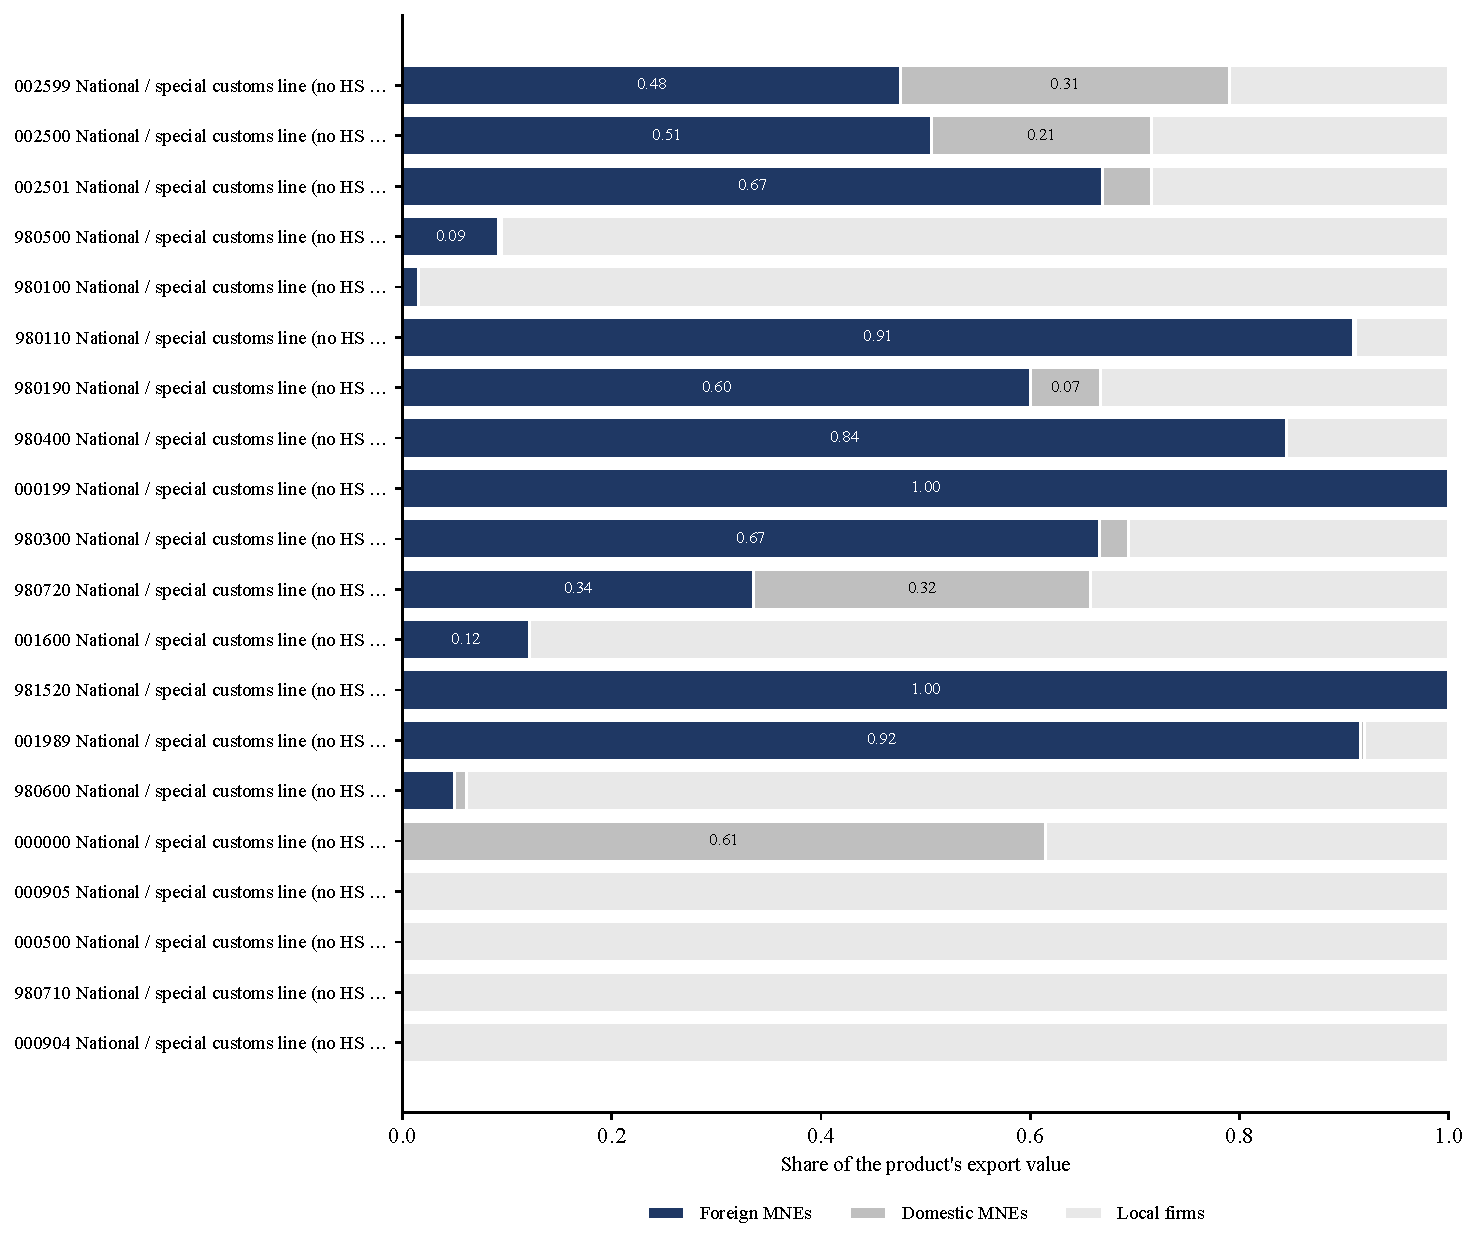
\includegraphics[width=1.0\textwidth,height=0.8\textheight,keepaspectratio]{figures/rest/fig_wp1f_top20_hs6_stacked.pdf}%
  \caption{Other Goods: Ownership of the Twenty Largest Export Products}%
  \label{fig:hs_st_rest}%
  \par\vspace{2pt}%
  \parbox{0.92\textwidth}{\footnotesize %
  \textit{Notes:} Shares of each product's export value. Twenty largest HS6 products by export value.\\[3pt]%
  \textit{Source:} Authors' calculations based on customs data matched to Orbis and Dun \& Bradstreet.}%
  \end{figure}
% ---- Figure: Other Goods: Ownership of the Twenty Largest Export Products, by Parent Country
\begin{figure}[H]\centering%
  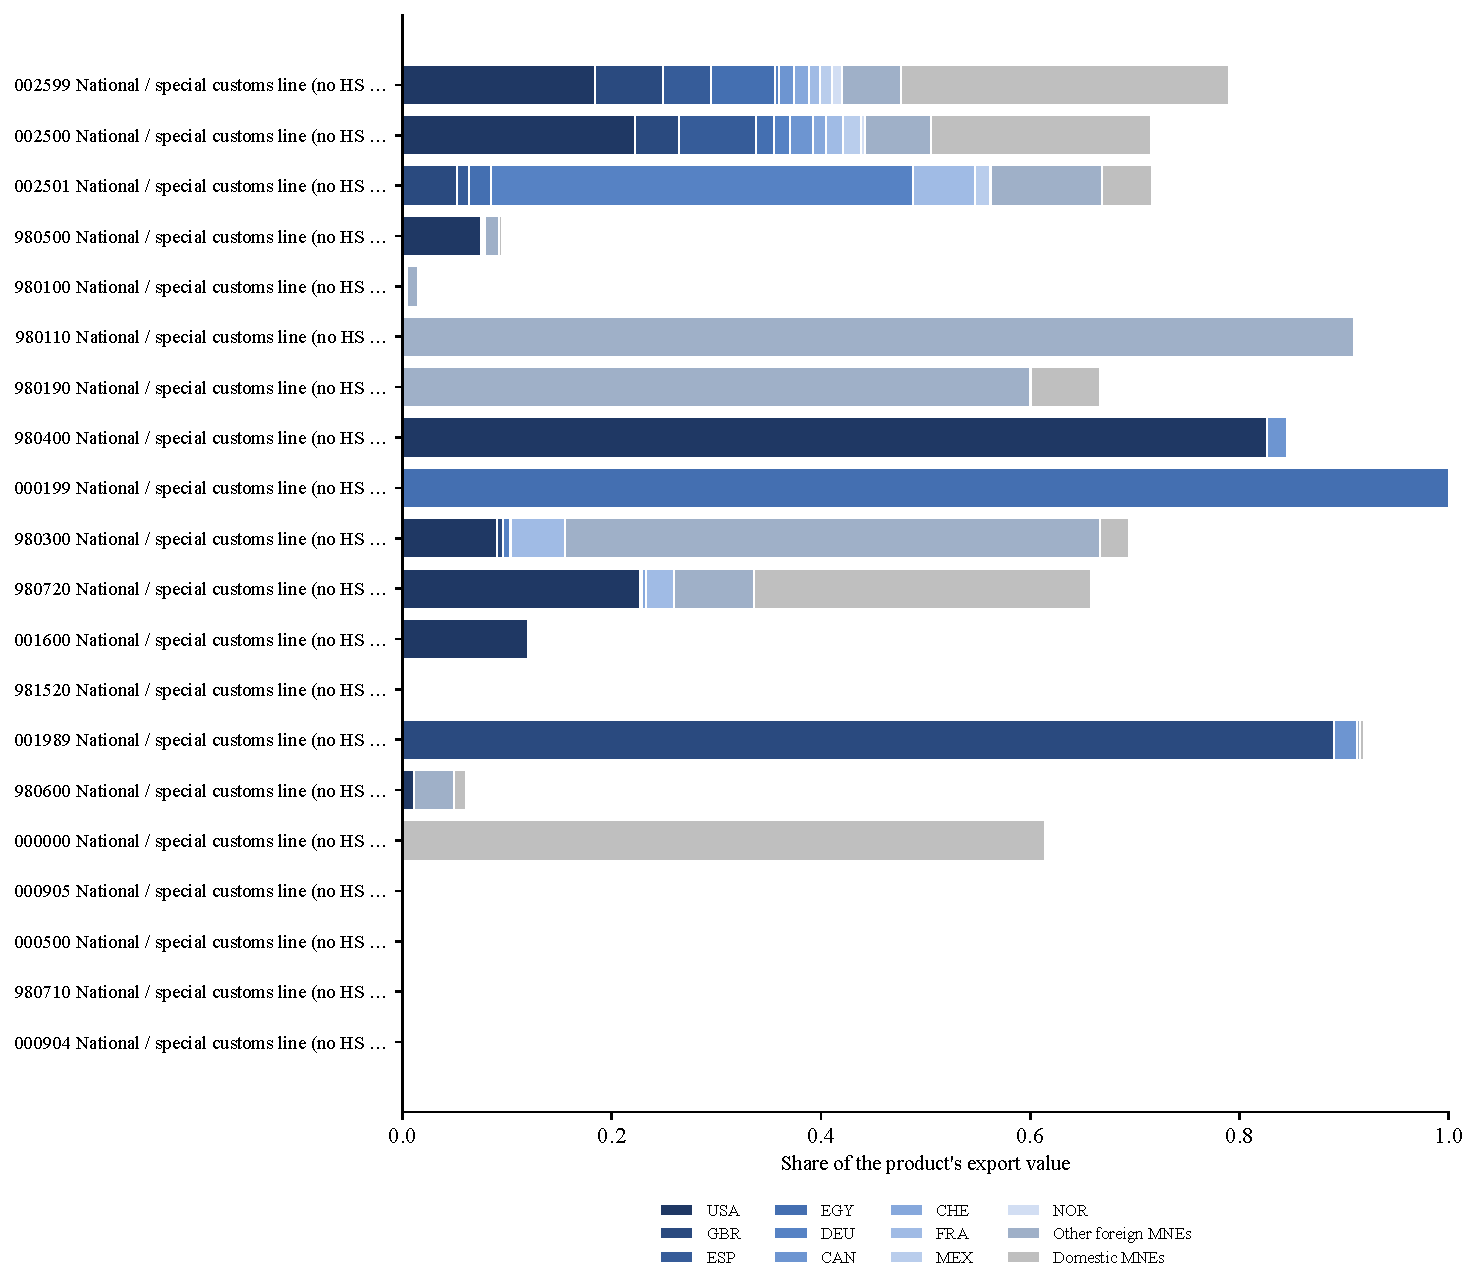
\includegraphics[width=1.0\textwidth,height=0.8\textheight,keepaspectratio]{figures/rest/fig_wp1f_top20_hs6_by_parent.pdf}%
  \caption{Other Goods: Ownership of the Twenty Largest Export Products, by Parent Country}%
  \label{fig:hs_par_rest}%
  \par\vspace{2pt}%
  \parbox{0.92\textwidth}{\footnotesize %
  \textit{Notes:} Shares of each product's export value. Foreign-MNE share split by country of the ultimate parent; the unfilled part of each bar is local firms.\\[3pt]%
  \textit{Source:} Authors' calculations based on customs data matched to Orbis and Dun \& Bradstreet.}%
  \end{figure}
% ---- Figure: Other Goods: Distribution of Export Value by Product-Level Foreign-Multinational Share
\begin{figure}[H]\centering%
  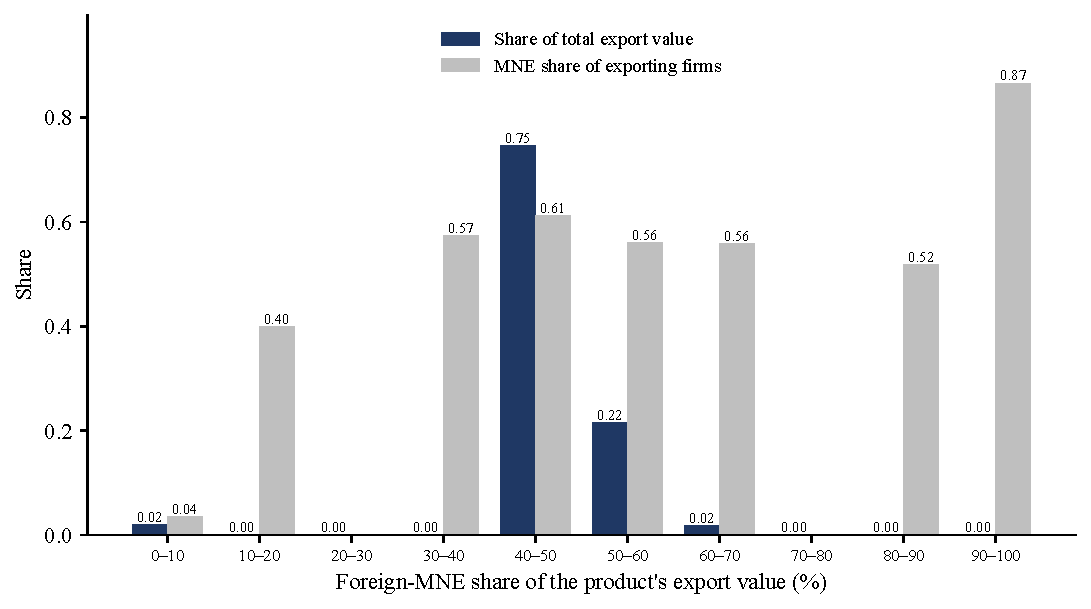
\includegraphics[width=0.85\textwidth,height=0.8\textheight,keepaspectratio]{figures/rest/fig_wp1f_foreign_share_distribution.pdf}%
  \caption{Other Goods: Distribution of Export Value by Product-Level Foreign-Multinational Share}%
  \label{fig:hs_dist_rest}%
  \par\vspace{2pt}%
  \parbox{0.92\textwidth}{\footnotesize %
  \textit{Notes:} Share of export value and MNE share of exporting firms, by the foreign-MNE share of each HS6 product's export value.\\[3pt]%
  \textit{Source:} Authors' calculations based on customs data matched to Orbis and Dun \& Bradstreet.}%
  \end{figure}
% ---- Table: Other Goods: Distribution of Export Value by Product-Level Foreign-Multinational Share
\begin{table}[H]\centering\small%
  \caption{Other Goods: Distribution of Export Value by Product-Level Foreign-Multinational Share}%
  \label{tab:hs_dist_t_rest}%
  \adjustbox{max width=\textwidth, max totalheight=0.8\textheight}{\begin{tabular}{lrrr}
\toprule
Foreign share bin (\%) & Share of value & MNE share of exporting firms & HS6 products \\
\midrule
0--10 & 0.019 & 0.036 & 13 \\
10--20 & 0.000 & 0.400 & 1 \\
20--30 & 0.000 & -- & 0 \\
30--40 & 0.000 & 0.573 & 1 \\
40--50 & 0.746 & 0.613 & 2 \\
50--60 & 0.215 & 0.560 & 1 \\
60--70 & 0.019 & 0.559 & 3 \\
70--80 & 0.000 & -- & 0 \\
80--90 & 0.000 & 0.519 & 1 \\
90--100 & 0.001 & 0.866 & 5 \\
\bottomrule
\end{tabular}
}%
  \par\vspace{3pt}%
  \begin{minipage}{0.95\textwidth}\footnotesize %
  \textit{Notes:} Share of export value and MNE share of exporting firms, by the foreign-MNE share of each HS6 product's export value. MNE share of exporting firms: MNE firm--destination--product--year observations over all observations in the bin.\\[3pt]%
  \textit{Source:} Authors' calculations based on customs data matched to Orbis and Dun \& Bradstreet.%
  \end{minipage}%
  \end{table}
% ---- Figure: Other Goods: Concentration of Exports across Products
\begin{figure}[H]\centering%
  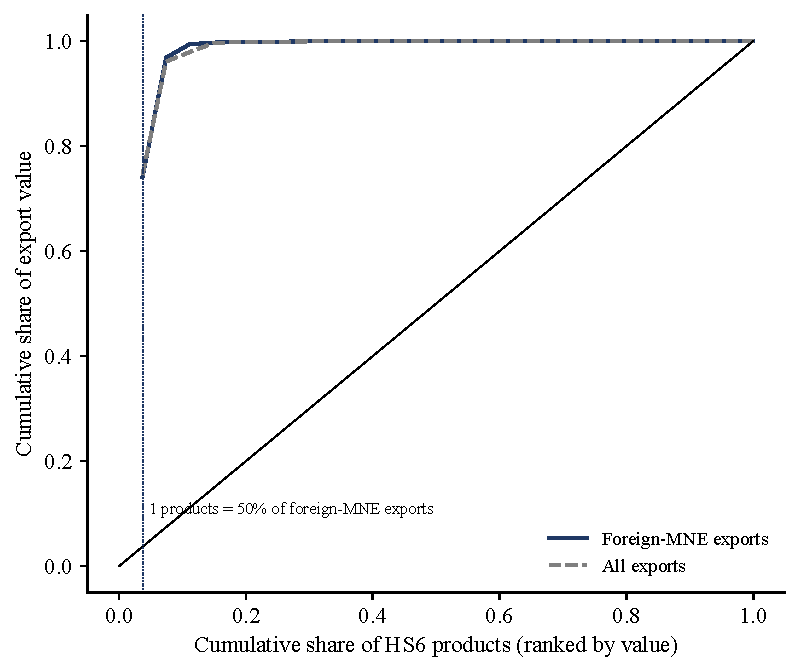
\includegraphics[width=0.6\textwidth,height=0.8\textheight,keepaspectratio]{figures/rest/fig_wp1f_lorenz_foreign.pdf}%
  \caption{Other Goods: Concentration of Exports across Products}%
  \label{fig:hs_lor_rest}%
  \par\vspace{2pt}%
  \parbox{0.92\textwidth}{\footnotesize %
  \textit{Notes:} Cumulative share of export value against the cumulative share of HS6 products, ranked by value, for foreign-MNE exports and for all exports.\\[3pt]%
  \textit{Source:} Authors' calculations based on customs data matched to Orbis and Dun \& Bradstreet.}%
  \end{figure}
% ---- Table: Other Goods: Exports and Multinational Shares, by HS Section
\begin{table}[H]\centering\footnotesize%
  \caption{Other Goods: Exports and Multinational Shares, by HS Section}%
  \label{tab:hs_sec_rest}%
  \adjustbox{max width=\textwidth, max totalheight=0.8\textheight}{\begin{tabular}{@{}p{7.2cm} r r r r l@{}}
\toprule
HS section & US\$bn/yr & Foreign (\%) & Domestic (\%) & Local (\%) & Leading parent \\
\midrule
Unclassified & 0.5 & 49 & 29 & 23 & USA (0.39) \\
Special / unclassified (98-99) & 0.0 & 13 & 1 & 87 & USA (0.57) \\
\midrule
All sections & 0.5 & 48 & 28 & 24 & \\
\bottomrule
\end{tabular}
}%
  \par\vspace{3pt}%
  \begin{minipage}{0.95\textwidth}\footnotesize %
  \textit{Notes:} Foreign, domestic and local: percent of each section's export value. Leading parent: largest parent country and its share of the section's foreign-MNE exports. Values are annual averages in US\$ billion.\\[3pt]%
  \textit{Source:} Authors' calculations based on customs data matched to Orbis and Dun \& Bradstreet.%
  \end{minipage}%
  \end{table}
% ---- Table: Other Goods: Thirty Largest Export Products
\begin{table}[H]\centering\footnotesize%
  \caption{Other Goods: Thirty Largest Export Products}%
  \label{tab:hs_by_value_rest}%
  \adjustbox{max width=\textwidth, max totalheight=0.8\textheight}{\begin{tabular}{@{}l p{6.4cm} r r r r l@{}}
\toprule
HS6 & Description & US\$bn/yr & Foreign (\%) & Domestic (\%) & Local (\%) & Leading parent \\
\midrule
002599 & National /\allowbreak{} special customs line (no HS description) & 0.36 & 48 & 31 & 21 & USA (0.39) \\
002500 & National /\allowbreak{} special customs line (no HS description) & 0.11 & 51 & 21 & 28 & USA (0.44) \\
002501 & National /\allowbreak{} special customs line (no HS description) & 0.01 & 67 & 5 & 28 & DEU (0.60) \\
980500 & National /\allowbreak{} special customs line (no HS description) & 0.01 & 9 & 0 & 91 & USA (0.82) \\
980100 & National /\allowbreak{} special customs line (no HS description) & 0.00 & 2 & 0 & 98 & PRY (0.32) \\
980110 & National /\allowbreak{} special customs line (no HS description) & 0.00 & 91 & 0 & 9 & JPN (1.00) \\
980190 & National /\allowbreak{} special customs line (no HS description) & 0.00 & 60 & 7 & 33 & JPN (1.00) \\
980400 & National /\allowbreak{} special customs line (no HS description) & 0.00 & 84 & 0 & 16 & USA (0.98) \\
000199 & National /\allowbreak{} special customs line (no HS description) & 0.00 & 100 & 0 & 0 & EGY (1.00) \\
980300 & National /\allowbreak{} special customs line (no HS description) & 0.00 & 67 & 3 & 31 & ALB (0.55) \\
980720 & National /\allowbreak{} special customs line (no HS description) & 0.00 & 34 & 32 & 34 & USA (0.68) \\
001600 & National /\allowbreak{} special customs line (no HS description) & 0.00 & 12 & 0 & 88 & USA (0.99) \\
981520 & National /\allowbreak{} special customs line (no HS description) & 0.00 & 100 & 0 & 0 & -- \\
001989 & National /\allowbreak{} special customs line (no HS description) & 0.00 & 92 & 0 & 8 & GBR (0.97) \\
980600 & National /\allowbreak{} special customs line (no HS description) & 0.00 & 5 & 1 & 94 & HUN (0.67) \\
000000 & National /\allowbreak{} special customs line (no HS description) & 0.00 & 0 & 61 & 39 & -- \\
000905 & National /\allowbreak{} special customs line (no HS description) & 0.00 & 0 & 0 & 100 & -- \\
000500 & National /\allowbreak{} special customs line (no HS description) & 0.00 & 0 & 0 & 100 & -- \\
980710 & National /\allowbreak{} special customs line (no HS description) & 0.00 & 0 & 0 & 100 & -- \\
000904 & National /\allowbreak{} special customs line (no HS description) & 0.00 & 0 & 0 & 100 & -- \\
000901 & National /\allowbreak{} special customs line (no HS description) & 0.00 & 47 & 0 & 53 & GBR (1.00) \\
980900 & National /\allowbreak{} special customs line (no HS description) & 0.00 & 0 & 0 & 100 & -- \\
001400 & National /\allowbreak{} special customs line (no HS description) & 0.00 & 100 & 0 & 0 & -- \\
980200 & National /\allowbreak{} special customs line (no HS description) & 0.00 & 0 & 0 & 100 & -- \\
002102 & National /\allowbreak{} special customs line (no HS description) & 0.00 & 0 & 0 & 100 & -- \\
981000 & National /\allowbreak{} special customs line (no HS description) & 0.00 & 0 & 0 & 100 & -- \\
000802 & National /\allowbreak{} special customs line (no HS description) & 0.00 & 0 & 0 & 100 & -- \\
\bottomrule
\end{tabular}
}%
  \par\vspace{3pt}%
  \begin{minipage}{0.95\textwidth}\footnotesize %
  \textit{Notes:} Thirty largest HS6 products by export value. Foreign, domestic and local: percent of the product's export value. Leading parent: largest parent country and its share of the product's foreign-MNE exports. Values are annual averages in US\$ billion.\\[3pt]%
  \textit{Source:} Authors' calculations based on customs data matched to Orbis and Dun \& Bradstreet.%
  \end{minipage}%
  \end{table}
% ---- Table: Other Goods: Thirty Largest Export Products of Foreign Multinationals
\begin{table}[H]\centering\footnotesize%
  \caption{Other Goods: Thirty Largest Export Products of Foreign Multinationals}%
  \label{tab:hs_by_foreign_value_rest}%
  \adjustbox{max width=\textwidth, max totalheight=0.8\textheight}{\begin{tabular}{@{}l p{6.4cm} r r r r l@{}}
\toprule
HS6 & Description & US\$bn/yr & Foreign (\%) & Domestic (\%) & Local (\%) & Leading parent \\
\midrule
002599 & National /\allowbreak{} special customs line (no HS description) & 0.36 & 48 & 31 & 21 & USA (0.39) \\
002500 & National /\allowbreak{} special customs line (no HS description) & 0.11 & 51 & 21 & 28 & USA (0.44) \\
002501 & National /\allowbreak{} special customs line (no HS description) & 0.01 & 67 & 5 & 28 & DEU (0.60) \\
980500 & National /\allowbreak{} special customs line (no HS description) & 0.01 & 9 & 0 & 91 & USA (0.82) \\
980110 & National /\allowbreak{} special customs line (no HS description) & 0.00 & 91 & 0 & 9 & JPN (1.00) \\
980400 & National /\allowbreak{} special customs line (no HS description) & 0.00 & 84 & 0 & 16 & USA (0.98) \\
980190 & National /\allowbreak{} special customs line (no HS description) & 0.00 & 60 & 7 & 33 & JPN (1.00) \\
000199 & National /\allowbreak{} special customs line (no HS description) & 0.00 & 100 & 0 & 0 & EGY (1.00) \\
980300 & National /\allowbreak{} special customs line (no HS description) & 0.00 & 67 & 3 & 31 & ALB (0.55) \\
980100 & National /\allowbreak{} special customs line (no HS description) & 0.00 & 2 & 0 & 98 & PRY (0.32) \\
981520 & National /\allowbreak{} special customs line (no HS description) & 0.00 & 100 & 0 & 0 & -- \\
980720 & National /\allowbreak{} special customs line (no HS description) & 0.00 & 34 & 32 & 34 & USA (0.68) \\
001989 & National /\allowbreak{} special customs line (no HS description) & 0.00 & 92 & 0 & 8 & GBR (0.97) \\
001600 & National /\allowbreak{} special customs line (no HS description) & 0.00 & 12 & 0 & 88 & USA (0.99) \\
000901 & National /\allowbreak{} special customs line (no HS description) & 0.00 & 47 & 0 & 53 & GBR (1.00) \\
980600 & National /\allowbreak{} special customs line (no HS description) & 0.00 & 5 & 1 & 94 & HUN (0.67) \\
001400 & National /\allowbreak{} special customs line (no HS description) & 0.00 & 100 & 0 & 0 & -- \\
002102 & National /\allowbreak{} special customs line (no HS description) & 0.00 & 0 & 0 & 100 & -- \\
000905 & National /\allowbreak{} special customs line (no HS description) & 0.00 & 0 & 0 & 100 & -- \\
000904 & National /\allowbreak{} special customs line (no HS description) & 0.00 & 0 & 0 & 100 & -- \\
980200 & National /\allowbreak{} special customs line (no HS description) & 0.00 & 0 & 0 & 100 & -- \\
000802 & National /\allowbreak{} special customs line (no HS description) & 0.00 & 0 & 0 & 100 & -- \\
000500 & National /\allowbreak{} special customs line (no HS description) & 0.00 & 0 & 0 & 100 & -- \\
980710 & National /\allowbreak{} special customs line (no HS description) & 0.00 & 0 & 0 & 100 & -- \\
980900 & National /\allowbreak{} special customs line (no HS description) & 0.00 & 0 & 0 & 100 & -- \\
981000 & National /\allowbreak{} special customs line (no HS description) & 0.00 & 0 & 0 & 100 & -- \\
000000 & National /\allowbreak{} special customs line (no HS description) & 0.00 & 0 & 61 & 39 & -- \\
\bottomrule
\end{tabular}
}%
  \par\vspace{3pt}%
  \begin{minipage}{0.95\textwidth}\footnotesize %
  \textit{Notes:} Thirty largest HS6 products by foreign-MNE export value. Foreign, domestic and local: percent of the product's export value. Leading parent: largest parent country and its share of the product's foreign-MNE exports. Values are annual averages in US\$ billion.\\[3pt]%
  \textit{Source:} Authors' calculations based on customs data matched to Orbis and Dun \& Bradstreet.%
  \end{minipage}%
  \end{table}
% ---- Table: Other Goods: Products with the Highest Foreign-Multinational Share
\begin{table}[H]\centering\footnotesize%
  \caption{Other Goods: Products with the Highest Foreign-Multinational Share}%
  \label{tab:hs_by_foreign_share_rest}%
  \adjustbox{max width=\textwidth, max totalheight=0.8\textheight}{\begin{tabular}{@{}l p{6.4cm} r r r r l@{}}
\toprule
HS6 & Description & US\$bn/yr & Foreign (\%) & Domestic (\%) & Local (\%) & Leading parent \\
\midrule
002500 & National /\allowbreak{} special customs line (no HS description) & 0.11 & 51 & 21 & 28 & USA (0.44) \\
002599 & National /\allowbreak{} special customs line (no HS description) & 0.36 & 48 & 31 & 21 & USA (0.39) \\
\bottomrule
\end{tabular}
}%
  \par\vspace{3pt}%
  \begin{minipage}{0.95\textwidth}\footnotesize %
  \textit{Notes:} HS6 products with exports of at least US\$500 million over the period, ranked by foreign-MNE share. Foreign, domestic and local: percent of the product's export value. Leading parent: largest parent country and its share of the product's foreign-MNE exports. Values are annual averages in US\$ billion.\\[3pt]%
  \textit{Source:} Authors' calculations based on customs data matched to Orbis and Dun \& Bradstreet.%
  \end{minipage}%
  \end{table}
% ---- Table: Other Goods: Products with the Highest Domestic-Multinational Share
\begin{table}[H]\centering\footnotesize%
  \caption{Other Goods: Products with the Highest Domestic-Multinational Share}%
  \label{tab:hs_by_domestic_share_rest}%
  \adjustbox{max width=\textwidth, max totalheight=0.8\textheight}{\begin{tabular}{@{}l p{6.4cm} r r r r l@{}}
\toprule
HS6 & Description & US\$bn/yr & Foreign (\%) & Domestic (\%) & Local (\%) & Leading parent \\
\midrule
002599 & National /\allowbreak{} special customs line (no HS description) & 0.36 & 48 & 31 & 21 & USA (0.39) \\
002500 & National /\allowbreak{} special customs line (no HS description) & 0.11 & 51 & 21 & 28 & USA (0.44) \\
\bottomrule
\end{tabular}
}%
  \par\vspace{3pt}%
  \begin{minipage}{0.95\textwidth}\footnotesize %
  \textit{Notes:} HS6 products with exports of at least US\$500 million over the period, ranked by domestic-MNE share. Foreign, domestic and local: percent of the product's export value. Leading parent: largest parent country and its share of the product's foreign-MNE exports. Values are annual averages in US\$ billion.\\[3pt]%
  \textit{Source:} Authors' calculations based on customs data matched to Orbis and Dun \& Bradstreet.%
  \end{minipage}%
  \end{table}

\section{Product Groups within the Sector}\label{sec:sub_rest}

\subsection{By HS Section}
% ---- Table: Other Goods: Exports and Multinational Shares, by HS Section
\begin{table}[H]\centering\footnotesize%
  \caption{Other Goods: Exports and Multinational Shares, by HS Section}%
  \label{tab:sc_hs_section_rest}%
  \adjustbox{max width=\textwidth, max totalheight=0.8\textheight}{\begin{tabular}{@{}l r r r r l@{}}
\toprule
HS section & Total exports (US\$bn/yr) & MNE exports (US\$bn/yr) & Foreign (\%) & Domestic (\%) & Leading parents (share of foreign) \\
\midrule
Special / unclassified (98-99) & 0.0 & 0.0 & 12.8 & 0.5 & USA 0.57, JPN 0.28, ALB 0.03 \\
Unclassified & 0.5 & 0.4 & 48.6 & 28.6 & USA 0.39, GBR 0.12, ESP 0.11 \\
\midrule
All & 0.5 & 0.4 & 47.9 & 28.0 & \\
\bottomrule
\end{tabular}
}%
  \par\vspace{3pt}%
  \begin{minipage}{0.95\textwidth}\footnotesize %
  \textit{Notes:} HS sections. Foreign and domestic: percent of the group's export value. Leading parents: the three largest parent countries and their share of the row's foreign-MNE exports. Values are annual averages in US\$ billion.\\[3pt]%
  \textit{Source:} Authors' calculations based on customs data matched to Orbis and Dun \& Bradstreet.%
  \end{minipage}%
  \end{table}
% ---- Figure: Other Goods: Multinational Share of Export Value, by HS Section
\begin{figure}[H]\centering%
  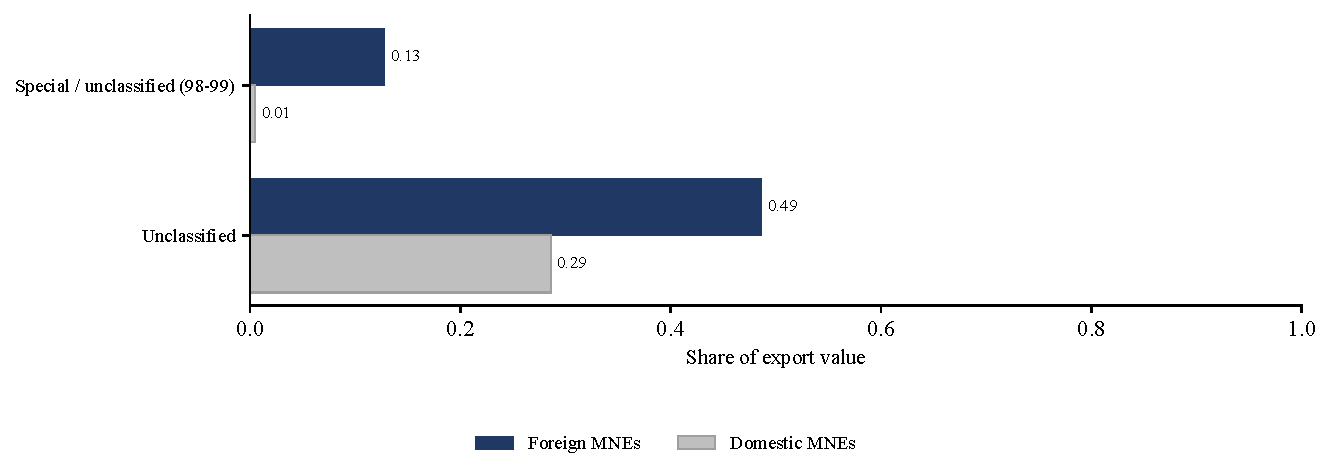
\includegraphics[width=0.9\textwidth,height=0.8\textheight,keepaspectratio]{figures/rest/fig_wp2_hs_section.pdf}%
  \caption{Other Goods: Multinational Share of Export Value, by HS Section}%
  \label{fig:sc_hs_section_f_rest}%
  \par\vspace{2pt}%
  \parbox{0.92\textwidth}{\footnotesize %
  \textit{Notes:} Shares of export value of other goods (HS 98--99 and unclassified codes), all available years pooled. HS sections.\\[3pt]%
  \textit{Source:} Authors' calculations based on customs data matched to Orbis and Dun \& Bradstreet.}%
  \end{figure}
% ---- Figure: Other Goods: Foreign-Multinational Share of Export Value, by Exporting Country and HS Section
\begin{figure}[H]\centering%
  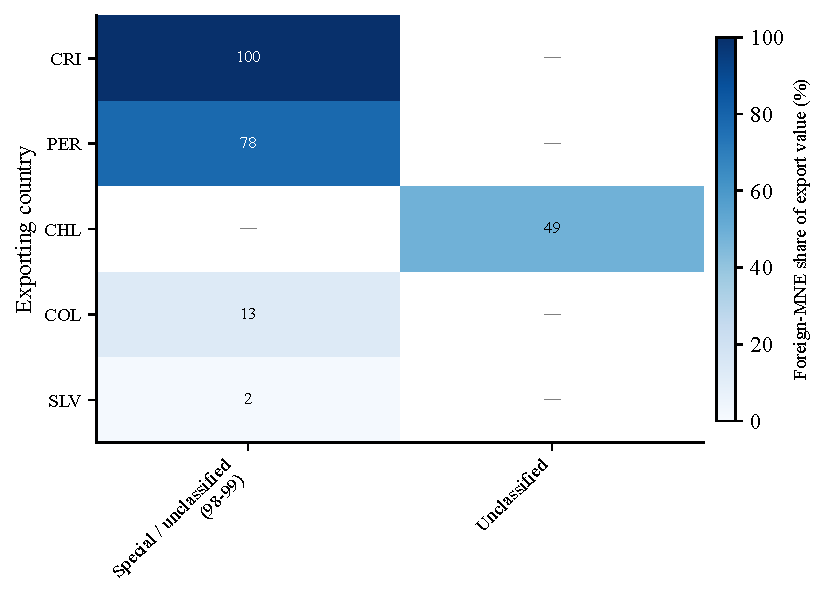
\includegraphics[width=0.95\textwidth,height=0.8\textheight,keepaspectratio]{figures/rest/fig_wp2_origin_x_hs_section.pdf}%
  \caption{Other Goods: Foreign-Multinational Share of Export Value, by Exporting Country and HS Section}%
  \label{fig:sc_hs_section_hm_rest}%
  \par\vspace{2pt}%
  \parbox{0.92\textwidth}{\footnotesize %
  \textit{Notes:} Percent of each group's export value in each country shipped by foreign MNEs. HS sections.\\[3pt]%
  \textit{Source:} Authors' calculations based on customs data matched to Orbis and Dun \& Bradstreet.}%
  \end{figure}
% ---- Table: Other Goods: Exports by Exporting Country and HS Section
\begin{table}[H]\centering\footnotesize%
  \caption{Other Goods: Exports by Exporting Country and HS Section}%
  \label{tab:sc_hs_section_ht_rest}%
  \adjustbox{max width=\textwidth, max totalheight=0.8\textheight}{\begin{tabular}{lrrr}
\toprule
Origin & Special / unclassified (98-99) & Unclassified & All \\
\midrule
\multicolumn{4}{l}{\textit{Panel A: composition of the origin's exports, \% (rows sum to 100)}} \\
CHL & 0.0 & 100.0 & 100.0 \\
COL & 100.0 & 0.0 & 100.0 \\
CRI & 100.0 & 0.0 & 100.0 \\
PER & 100.0 & 0.0 & 100.0 \\
SLV & 100.0 & 0.0 & 100.0 \\
All origins & 2.1 & 97.9 & 100.0 \\
\midrule
\multicolumn{4}{l}{\textit{Panel B: foreign-MNE share of export value, \%}} \\
CHL & -- & 48.6 & 48.6 \\
COL & 12.7 & -- & 12.7 \\
CRI & 100.0 & -- & 100.0 \\
PER & 78.0 & -- & 78.0 \\
SLV & 1.5 & -- & 1.5 \\
All origins & 12.8 & 48.6 & 47.9 \\
\bottomrule
\end{tabular}
}%
  \par\vspace{3pt}%
  \begin{minipage}{0.95\textwidth}\footnotesize %
  \textit{Notes:} Panel A: composition of each country's exports in the sector (rows add to 100). Panel B: percent of each cell's export value shipped by foreign MNEs. HS sections.\\[3pt]%
  \textit{Source:} Authors' calculations based on customs data matched to Orbis and Dun \& Bradstreet.%
  \end{minipage}%
  \end{table}
% ---- Table: Other Goods: Exports by HS Section and Parent Country
\begin{table}[H]\centering\footnotesize%
  \caption{Other Goods: Exports by HS Section and Parent Country}%
  \label{tab:sc_hs_section_par_rest}%
  \adjustbox{max width=\textwidth, max totalheight=0.8\textheight}{\begin{tabular}{lrrrrrrrrrrrr}
\toprule
HS section & USA & GBR & ESP & EGY & DEU & CAN & CHE & FRA & MEX & NOR & Other & Domestic \\
\midrule
Special / unclassified (98-99) & 5.8 & 0.0 & 0.1 & 0.0 & 0.0 & 0.0 & 0.0 & 0.1 & 0.0 & 0.0 & 6.7 & 0.5 \\
Unclassified & 15.3 & 4.8 & 4.2 & 4.0 & 1.3 & 1.3 & 1.1 & 1.1 & 1.0 & 0.7 & 14.0 & 28.6 \\
\bottomrule
\end{tabular}
}%
  \par\vspace{3pt}%
  \begin{minipage}{0.95\textwidth}\footnotesize %
  \textit{Notes:} Percent of each group's export value, by country of the ultimate parent of foreign MNEs; domestic MNEs shown for comparison. HS sections.\\[3pt]%
  \textit{Source:} Authors' calculations based on customs data matched to Orbis and Dun \& Bradstreet.%
  \end{minipage}%
  \end{table}

\subsection{HS Section and End Use}
% ---- Table: Other Goods: Exports by HS Section and End Use
\begin{table}[H]\centering\small%
  \caption{Other Goods: Exports by HS Section and End Use}%
  \label{tab:sxe_v_rest}%
  \adjustbox{max width=\textwidth, max totalheight=0.8\textheight}{\begin{tabular}{lr}
\toprule
HS section / BEC end use & Total \\
\midrule
\midrule
Total & 0.0 \\
\bottomrule
\end{tabular}
}%
  \par\vspace{3pt}%
  \begin{minipage}{0.95\textwidth}\footnotesize %
  \textit{Notes:} Export value by HS section and BEC Rev.\,4 end use. Values are annual averages in US\$ billion.\\[3pt]%
  \textit{Source:} Authors' calculations based on customs data matched to Orbis and Dun \& Bradstreet.%
  \end{minipage}%
  \end{table}
% ---- Table: Other Goods: Foreign-Multinational Share of Exports by HS Section and End Use
\begin{table}[H]\centering\small%
  \caption{Other Goods: Foreign-Multinational Share of Exports by HS Section and End Use}%
  \label{tab:sxe_f_rest}%
  \adjustbox{max width=\textwidth, max totalheight=0.8\textheight}{\begin{tabular}{l}
\toprule
HS section / BEC end use \\
\midrule
\bottomrule
\end{tabular}
}%
  \par\vspace{3pt}%
  \begin{minipage}{0.95\textwidth}\footnotesize %
  \textit{Notes:} Percent of each cell's export value shipped by foreign MNEs.\\[3pt]%
  \textit{Source:} Authors' calculations based on customs data matched to Orbis and Dun \& Bradstreet.%
  \end{minipage}%
  \end{table}
\end{document}
